\documentclass{article}


% if you need to pass options to natbib, use, e.g.:
\PassOptionsToPackage{numbers, compress}{natbib}
% before loading neurips_2024


% ready for submission
\usepackage{neurips_2024}


% to compile a preprint version, e.g., for submission to arXiv, add add the
% [preprint] option:
%     \usepackage[preprint]{neurips_2024}


% to compile a camera-ready version, add the [final] option, e.g.:
%     \usepackage[final]{neurips_2024}


% to avoid loading the natbib package, add option nonatbib:
%    \usepackage[nonatbib]{neurips_2024}


\usepackage[utf8]{inputenc} % allow utf-8 input
\usepackage[T1]{fontenc}    % use 8-bit T1 fonts
\usepackage{amsthm, amsmath, amsfonts, amssymb, bm, bbm} % Math packages
\usepackage{graphicx}
\usepackage{url}            % simple URL typesetting
\usepackage{booktabs}       % professional-quality tables
\usepackage{amsfonts}       % blackboard math symbols
\usepackage{nicefrac}       % compact symbols for 1/2, etc.
\usepackage{microtype}      % microtypography
\usepackage{xcolor}         % colors
\usepackage[labelfont={small,bf},textfont={small},labelsep=space,tableposition=top]{caption}
\usepackage{subcaption}
\usepackage[ruled,linesnumbered,vlined]{algorithm2e}
\usepackage[colorlinks=true, allcolors=blue]{hyperref}
\usepackage{fixltx2e}
\usepackage{pgf}
\usepackage{tikz}

\usepackage{mathtools}
\usepackage{xargs}
\usepackage{soul}

\DeclareMathOperator\prox{prox}%											proximal mapping
\DeclareMathOperator*\minimize{minimize}%									minimize


\newcommand{\N}{\mathbb N}%												    naturals
\newcommand{\Z}{\mathbb Z}%												    naturals
\newcommand{\R}{\mathbb{R}}
\newcommand{\func}[3]{#1:#2\rightarrow#3}%									f: A --> B function \func{f}{A}{B}


\newcommandx\seq[3][{2=k\in\N},{3={}}]{(#1)_{#2}^{#3}}%						sequence \seq{x^k}[k=1][n]


\newtheorem{ass}{Assumption}
\newtheorem{prop}{Proposition}
\newtheorem{remark}{Remark}
\newtheorem{lem}{Lemma}


\newcounter{mysubequations}
\renewcommand{\themysubequations}{(\alph{mysubequations})}
\newcommand{\mysubnumber}{\refstepcounter{mysubequations}\themysubequations}

\newcommand{\pourya}[1]{{\color{blue}{#1}}}


\newtheorem{theorem}{Theorem}
\DeclareMathOperator*{\argmin}{arg\,min}
\DeclareMathOperator*{\argmax}{arg\,max}
\DeclareMathOperator{\clamp}{clamp}
\DeclareMathOperator{\round}{round}


\title{Quantization-free Lossy Image Compression Using Integer Matrix Factorization}


% The \author macro works with any number of authors. There are two commands
% used to separate the names and addresses of multiple authors: \And and \AND.
%
% Using \And between authors leaves it to LaTeX to determine where to break the
% lines. Using \AND forces a line break at that point. So, if LaTeX puts 3 of 4
% authors names on the first line, and the last on the second line, try using
% \AND instead of \And before the third author name.


\author{%
Pooya Ashtari$^{1}$\thanks{Corresponding author. Emails: \texttt{pooya.ashtari@esat.kuleuven.be}, \texttt{pooya.ash@gmail.com}}\ \ \thanks{Equal contribution} \\
\texttt{pooya.ashtari@esat.kuleuven.be} \\
\vspace{-20pt}
\And
Pourya Behmandpoor$^{1}$\footnotemark[2] \\
\texttt{pourya.behmandpoor@kuleuven.be} \\
\vspace{-20pt}
\And
Fateme Nateghi Haredasht$^{2}$ \\
\texttt{fnateghi@stanford.edu} \\
\vspace{-20pt}
\And
Jonathan H. Chen$^{2}$ \\
\texttt{jonc101@stanford.edu} \\
\vspace{-20pt}
\And
Panagiotis Patrinos$^{1}$ \\
\texttt{panos.patrinos@esat.kuleuven.be} \\
\And
Sabine Van Huffel$^{1}$ \\
\texttt{sabine.vanhuffel@kuleuven.be} \\
\And
\vspace{-20pt} \\
\small{$^{1}$Department of Electrical Engineering (ESAT), STADIUS Center, KU Leuven, Belgium} \\
\small{$^{2}$Stanford Center for Biomedical Informatics Research, Stanford University, CA, USA} \\
  % examples of more authors
  % \And
  % Coauthor \\
  % Affiliation \\
  % Address \\
  % \texttt{email} \\
  % \AND
  % Coauthor \\
  % Affiliation \\
  % Address \\
  % \texttt{email} \\
  % \And
  % Coauthor \\
  % Affiliation \\
  % Address \\
  % \texttt{email} \\
  % \And
  % Coauthor \\
  % Affiliation \\
  % Address \\
  % \texttt{email} \\
}


\begin{document}


\maketitle


\begin{abstract}
Image compression is essential for efficient transmission and storage.The most widely used transform coders, such as the discrete cosine transform (DCT) and singular value decomposition (SVD), represent image data in continuous domains, necessitating carefully designed quantizers. Notably, the performance of SVD-based methods is more sensitive to quantization errors than that of DCT-based methods like JPEG. Therefore, we introduce a variant of integer matrix factorization (IMF) to develop a novel quantization-free image compression method. IMF provides a low-rank representation of the image data as a product of two smaller factor matrices with bounded integer elements, thereby eliminating the need for quantization. We propose an efficient, provably convergent iterative algorithm for IMF using a block coordinate descent (BCD) scheme, with subproblems having closed-form solutions. The experiments demonstrate that our IMF-based compression method outperforms JPEG, achieving improvements of over 3 dB in PSNR at rates of under 0.17 bits per pixel (bpp) on the Kodak dataset. We also assessed our method's capability to preserve visual semantic information by evaluating an ImageNet pre-trained classifier on compressed images. Remarkably, our method resulted in an improvement of over 10\% in top-1 accuracy compared to JPEG at rates under 0.23 bpp.
\end{abstract}

\section{Introduction} \label{sec:introduction}

Lossy image compression involves reducing the storage size of digital images by discarding some image data that are redundant or less perceptible to the human eye. This is crucial for efficiently storing and transmitting images, particularly in applications where bandwidth or storage resources are limited, such as web browsing, streaming, and mobile platforms. Lossy image compression methods enable adjusting the degree of compression, providing a selectable tradeoff between storage size and image quality. Widely used methods such as JPEG \cite{wallace1991jpeg} and JPEG 2000 \cite{skodras2001jpeg} follow the \emph{transform coding} paradigm \cite{goyal2001theoretical}. They use orthogonal linear transformations, such as discrete cosine transform (DCT) \cite{ahmed1974discrete} and discrete wavelet transform (DWT) \cite{antonini1992image}, to decorrelate small image blocks. Since these transforms map image data into a continuous domain, quantization is necessary before coding into bytes. Unfortunately, as quantization errors can significantly degrade compression performance, the quantizers must be carefully crafted to minimize this impact, which further complicates codec design.

Another promising paradigm relies on low-rank approximation techniques, with singular value decomposition (SVD) being a notable example. SVD is recognized as the deterministically optimal transform for energy compaction \cite{andrews1976singular}. In practice, current SVD-based methods \cite{andrews1976singular, prasantha2007image, hou2015sparse} can represent image data only with factors that contain floating-point elements, necessitating a quantization step prior to any byte-level processing. \revise{The quantization step often introduces errors, which result in suboptimal compression performance.}

\revise{Motivated by this, we introduce a new variant of integer matrix factorization (IMF) and, based on it, develop an effective lossy image compression method. Unlike traditional compression methods, the proposed approach integrates quantization into the optimization process rather than treating it as a separate step before byte-level processing. Our IMF formulation provides a low-rank representation of image data as the product of two smaller factor matrices. The quantization is integrated via introducing constraints in the optimization process, where the elements of the factor matrices are constrained to \emph{bounded integer} values. These elements, with discrete values represented as bounded integers, can be directly stored using standard integral data types---such as \texttt{int8} and \texttt{int16} supported by programming languages---and losslessly processed, making IMF arguably better suited than SVD for image compression.} Another advantage of IMF is that the reshaped factor matrices can be treated as 8-bit grayscale images, allowing any lossless image compression standard to be seamlessly integrated into the proposed framework. We propose an efficient iterative algorithm for IMF using a block coordinate descent (BCD) scheme, where each column of a factor matrix is taken as a block and updated one at a time using a closed-form solution.

Our contributions are summarized as follows. \revise{We propose a new IMF formulation that enables the integration of quantization and low-rank approximation for image compression.} Moreover, we introduce an efficient algorithm for the IMF problem and prove its convergence. Finally, to the best of our knowledge, this work is the first effort to explore IMF for image compression, presenting the first algorithm based on a low-rank approach that significantly outperforms SVD and competes favorably with JPEG, particularly at low bit rates. Our method narrows the gap between factorization and quantization by integrating them into a single layer and optimizing the compression system.

\section{Related Work} \label{sec:related_work}

\paragraph{Transform Coding}
Transform coding is a widely used approach in lossy image compression, leveraging mathematical transforms to decorrelate pixel values and represent image data more compactly. One of the earliest and most influential methods is the discrete cosine transform (DCT) \cite{ahmed1974discrete}, used in JPEG \cite{wallace1991jpeg}, which converts image data into the frequency domain, prioritizing lower frequencies to retain perceptually significant information. The discrete wavelet transform (DWT) \cite{antonini1992image}, used in JPEG 2000 \cite{skodras2001jpeg}, offers improved performance by capturing both frequency and location information, leading to better handling of edges and textures \cite{shapiro1993embedded}. More recently, the WebP \cite{google2011webp} and HEIF \cite{lainema2016hevc, hannuksela2015high} formats combine DCT and intra-frame prediction to achieve superior compression and quality compared to JPEG.

\paragraph{Learned Image Compression (LIC)}
Recently, learned image compression (LIC) has gained attention for potentially outperforming traditional methods by leveraging deep neural networks. \citet{balle2018variational} pioneered this area with an end-to-end trainable convolutional neural network based on variational autoencoders.\remove{Mentzer et al. (2020) ("High-fidelity generative image compression") integrated generative adversarial networks into LIC, developing an effective generative lossy compression system.} \citet{cheng2020learned} incorporated a simplified attention module and discretized Gaussian mixture likelihoods for achieving a more accurate and flexible entropy model. \citet{liu2023learned} combined transformers and CNNs to exploit the local modeling ability of convolutions and the global modeling ability of the attention mechanism. \citet{yang2024lossy} introduced diffusion models into LIC, using a denoising decoder to iteratively reconstruct a compressed image. Despite these advancements, the high computational complexity of LIC methods remains a significant limitation, particularly for real-time applications and resource-constrained environments.

\paragraph{Low-rank Techniques}
Low-rank approximation can provide a compact representation by decomposing image data into smaller components. Notably, truncated singular value decomposition (tSVD) is a classical technique that decomposes images into singular values and vectors, retaining only the most significant components to achieve compression \cite{andrews1976singular, prasantha2007image}. \citet{hou2015sparse} proposed sparse low-rank matrix approximation (SLRMA) for data compression, which is able to explore both the intra- and inter-coherence of data samples simultaneously from the perspective of optimization and transformation.
More recently, \citet{yuan2020image} introduced a graph-based low-rank regularization to reduce compression artifacts near block boundaries at low bit rates.

\paragraph{Integer Matrix Factorization}
There are applications where meaningful representation of data as discrete factor matrices is crucial. While typical low-rank techniques like SVD and nonnegative matrix factorization (NMF) are inappropriate for such applications, integer matrix factorization (IMF) ensures the integrality of factors to achieve this goal. \citet{lin2005integer} investigates IMF to effectively handle discrete data matrices for cluster analysis and pattern discovery. \citet{dong2018integer} introduce an alternative least squares method for IMF, verifying its effectiveness with some data mining applications. However, the application of IMF in image compression remains unexplored.

While existing IMF methods generally constrain factor elements to the entire set of integer values, we propose quantized matrix factorization (QMF), which minimizes the objective function over a bounded interval of integers, thereby modeling a uniformly quantized domain. Furthermore, we introduce a block coordinate descent (BCD)-based algorithm to solve the QMF problem, which is both computationally efficient and provably convergent. This work investigates the potential of QMF for image compression, arguing that it can serve as a powerful tool for this purpose.

\section{Method} \label{sec: method}



\subsection{Overall Framework} \label{sec: overall framework}

\begin{figure}[t]
	\centering
	\includegraphics[width=\linewidth]{figures/imf_encoder.pdf}
	\vspace{10pt}
	\caption{An illustration of the encoder for our image compression method, based on integer matrix factorization.}
	\label{fig:imf_encoder}
\end{figure}

Figure \ref{fig:imf_encoder} illustrates an overview of the encoding pipeline for our proposed image compression method using integer matrix factorization (IMF). The encoder accepts an RGB image with dimensions $H \times W$ and a color depth of 8 bits, represented by the tensor $\bm{\mathcal{X}} \in \{0, \ldots, 255\}^{3 \times H \times W}$. Each step of encoding is described in the following.

\paragraph{Color Space Transformation.}
Analogous to the JPEG standard, the image is initially transformed into the YC\textsubscript{B}C\textsubscript{R} color space. Let $\bm{Y} \in [0, 255]^{H \times W}$ represent the \emph{luma} component, and $\bm{C}_B, \bm{C}_R \in [0, 255]^{\frac{H}{2} \times \frac{W}{2}}$ represent the blue-difference and red-difference \emph{chroma} components, respectively. Note that as a result of this transformation, the elements of the \emph{luma} ($\bm{Y}$) and \emph{chroma} ($\bm{C}_B$, $\bm{C}_R$) matrices are not limited to integers and can take any value within the interval $[0, 255]$.

%\begin{equation} \label{eq: ycbcr transform}
%	\begin{bmatrix}
	%		Y \\
	%		C_B \\
	%		C_R
	%	\end{bmatrix} \triangleq
%	\begin{bmatrix}
	%		0.299 & 0.587 & 0.114 \\
	%		-0.168736 & -0.331264 & 0.5 \\
	%		0.5 & -0.418688 & -0.081312
	%	\end{bmatrix}
%	\begin{bmatrix}
	%		R \\
	%		G \\
	%		B
	%	\end{bmatrix}
%	+
%	\begin{bmatrix}
	%		0 \\
	%		128 \\
	%		128
	%	\end{bmatrix},
%\end{equation}

\paragraph{Chroma Downsampling.} 
After conversion to the YC\textsubscript{B}C\textsubscript{R} color space, the \emph{chroma} components $\bm{C}_B$ and $\bm{C}_R$ are downsampled using average-pooling with a kernel size of $(2, 2)$ and a stride of $(2, 2)$, similar to the process used in JPEG. This downsampling exploits the fact that the human visual system perceives far more detail in brightness information (\emph{luma}) than in color saturation ({chroma}).

\paragraph{Patchification.}
Following \emph{chroma} downsampling, we have three components:  the \emph{luma} component $\bm{Y} \in [0, 255]^{H \times W}$ and the \emph{chroma} components $\bm{C}_B, \bm{C}_R \in [0, 255]^{\frac{H}{2} \times \frac{W}{2}}$. Each of the matrices is split into non-overlapping $8 \times 8$ patches. If a dimension of a matrix is not divisible by 8, the matrix is first padded to the nearest size divisible by 8 using reflection of the boundary values. These patches are then flattened into row vectors and stacked vertically to form matrices $\bm{X}_{Y} \in [0, 255]^{\frac{HW}{64} \times 64}$, $\bm{X}_{C_B} \in [0, 255]^{\frac{HW}{256} \times 64}$, and $\bm{X}_{C_R} \in [0, 255]^{\frac{HW}{256} \times 64}$. Later, these matrices will be low-rank approximated using integer matrix factorization (IMF). Note that this patchification technique differs from the block splitting in JPEG, where each block is subject to discrete cosine transform (DCT) and processed independently. This patchification technique not only captures the locality and spatial dependencies of neighboring pixels but also performs better with the matrix decomposition approach to image compression.

\paragraph{Low-rank approximation.} 
We now apply a low-rank approximation to the matrices $\bm{X}_{Y}$, $\bm{X}_{C_B}$, and $\bm{X}_{C_R}$, which is the core of our compression method that provides a lossy compressed representation of these matrices.  The low-rank approximation \citep{eckart1936approximation} aims to approximate a given matrix $ \bm{X} \in \mathbb{R}^{M \times N} $ by 
\begin{equation} \label{eq: lra}
	\bm{X} \approx \bm{U} \bm{V}^\mathsf{T} = \sum_{r=1}^{R} U_{:r} {V_{:r}}^\mathsf{T},
\end{equation} 
where $\bm{U} \in \mathbb{R}^{M \times R}$ and $\bm{V} \in \mathbb{R}^{N \times R}$ are \emph{factor matrices} (or simply \emph{factors}), and $R \leq \min(M,N)$ represents the \emph{rank}. We refer to $\bm{U}$ as the \emph{basis matrix} and $\bm{V}$ as the \emph{coefficient matrix}. By selecting a sufficiently small value for $R$, the factor matrices $\bm{U}$ and $\bm{V}$, with a combined total of $(M+N)R$ elements, offer a compact representation of the original matrix $\bm{X}$, which has $MN$ elements, capturing the most significant patterns in the image. Depending on the loss function used to measure the reconstruction error between $\bm{X}$ and the product $\bm{U} \bm{V}^\mathsf{T}$, as well as the constraints on the factor matrices $\bm{U}$ and $\bm{V}$, various formulations and variants have been proposed for different purposes. In Section \ref{sec: imf}, we introduce and elaborate on our variant, termed integer matrix factorization (IMF), and argue why it is well-suited and effective for image compression. 

\paragraph{Reshape factors.} 
IMF yields integers factor matrices $\bm{U}_{Y} \in \{0, \ldots, 255\}^{\frac{HW}{64} \times R}$ and $\bm{V}_{Y} \in \{0, \ldots, 255\}^{64 \times R}$; $\bm{U}_{C_B} \in \{0, \ldots, 255\}^{\frac{HW}{256} \times R}$ and $\bm{V}_{C_B} \in \{0, \ldots, 255\}^{64 \times R}$; and $\bm{U}_{C_R} \in \{0, \ldots, 255\}^{\frac{HW}{256} \times R}$ and $\bm{V}_{C_R} \in \{0, \ldots, 255\}^{64 \times R}$ that correspond to $\bm{X}_{Y}$, $\bm{X}_{C_B}$, and $\bm{X}_{C_R}$. We reshape these matrices by unfolding their first dimension to obtain $R$-channel 2D spatial maps, referred to as \emph{factor maps} and represented by the following tensors:
\begin{align} \label{eq: reshaped factors}
	\bm{\mathcal{U}}_{Y} & \in \{0, \ldots, 255\}^{R \times \frac{H}{8} \times \frac{W}{8}}, \nonumber \\
	\bm{\mathcal{U}}_{C_B}, \bm{\mathcal{U}}_{C_R} & \in \{0, \ldots, 255\}^{R \times \frac{H}{16} \times \frac{W}{16}}, \nonumber \\
	\bm{\mathcal{V}}_{Y}, \bm{\mathcal{V}}_{C_B}, \bm{\mathcal{V}}_{C_R} & \in \{0, \ldots, 255\}^{R \times 8 \times 8}.
\end{align}

\paragraph{Lossless image compression.}
Since \emph{factor maps} are already integer tensors, we do not need a quantization step, which is commonly present in other lossy image compression methods and adds extra complications. This is the main advantage of our approach. Moreover, each channel of a \emph{factor map} can be treated as a 8-bit grayscale image and therefore can be directly encoded by any standard lossless image compression method, such as PNG or WebP. For images with a resolution of $H, W \gg 64$, which are most common nowadays, the basis maps ($\bm{\mathcal{U}}$) are significantly larger than the coefficient maps ($\bm{\mathcal{V}}$), accounting for the majority of the storage space. Interestingly, in practice, the IMF basis maps turn out to be meaningful images, each capturing some visual semantic of the image (see Figure \ref{fig:imf_components} for an example). Therefore, our IMF approach can effectively leverage the power of existing lossless image compression algorithms, offering a significant advantage over current methods.


\subsection{Integer Matrix Factorization (IMF)} \label{sec: imf}

The main building block of our method is integer matrix factorization (IMF), which is responsible for lossy compression of matrices obtained through patchification. IMF can be framed as an optimization problem, aiming to minimize the reconstruction error between the original matrix $\bm{X} \in \mathbb{R}^{M \times N}$ and the product $\bm{U} \bm{V}^\mathsf{T}$, while ensuring that the elements of the factor matrices $\bm{U}$ and $\bm{V}$ are integers within a specified interval $[\alpha,\beta]$. Formally, the IMF problem can be expressed as:
\begin{align} \label{eq: imf problem}
	\minimize_{\bm{U}, \bm{V}} & \ \  \| \bm{X} - \bm{U} \bm{V}^\mathsf{T} \|_\text{F}^2 \nonumber \\
	\text{s.t.}           & \ \ \bm{U} \in \mathbb{Z}_{[\alpha,\beta]}^{M \times R}, \bm{V} \in \mathbb{Z}_{[\alpha,\beta]}^{N \times R},
\end{align}
where $\|\cdot\|_\text{F}$ denotes the Frobenius norm; $R \leq \min(M,N)$ represents the \emph{rank}; and $\mathbb{Z}_{[\alpha,\beta]} \triangleq [\alpha,\beta] \cap \mathbb{Z}$ denotes the set of integers within $[\alpha,\beta]$. Without constraints on the factors, the problem would have an analytic solution through the singular value decomposition (SVD), as addressed by the Eckart–Young–Mirsky theorem \cite{eckart1936approximation}. If only a nonnegativity constraint were applied (without integrality), variations of nonnegative matrix factorization (NMF) would emerge \cite{lee2000algorithms, gillis2020nonnegative}. The IMF problem \eqref{eq: imf problem} poses a challenging integer program, with finding its global minima known to be NP-hard \cite{dong2018integer, van1981another}. Only a few iterative algorithms \cite{dong2018integer, lin2005integer} have been proposed to find a ``good solution" for some IMF variants in contexts other than image compression. In Section \ref{sec: bcd}, we propose an efficient iterative algorithm for the IMF problem \eqref{eq: imf problem}.

The application of SVD and NMF in image compression is problematic mainly because the resulting factors contain continuous values that must be represented as arrays of floating-point numbers. This necessitates a quantization step that not only adds extra complications but also significantly degrades compression performance due to quantization errors (as demonstrated in Section \ref{sec: experiments}). Conversely, our IMF formulation produces integer factor matrices that can be directly stored and losslessly processed without incurring roundoff errors. The reason for limiting the feasible region to $[\alpha,\beta]$ in our IMF formulation is to enable more compact storage of the factors using standard integral data types, such as \texttt{int8} and \texttt{int16}, supported by programming languages. Given that the elements of the input matrix $\bm{X}$ are in $[0, 255]$, we found the signed \texttt{int8} type, which represents integers from -128 to 127, suitable for image compression applications. As a result, our IMF formulation is well-suited for image compression, effectively integrating the factorization and quantization steps into a single, efficient compression process.


\subsection{Block Coordinate Descent Scheme for IMF} \label{sec: bcd}

We propose an efficient algorithm for IMF using the block coordinate descent (BCD) scheme (aka alternating optimization). Starting with some initial parameter values, this approach involves sequentially minimizing the cost function with respect to a single column of a factor at a time, while keeping the other columns of that factor and the entire other factor fixed. This process is repeated until a stopping criterion is met, such when the change in the cost function value falls below a predefined threshold or the maximum number of iterations is reached. Formally, this involves solving one of the following subproblems at a time:
\begin{align}  
	\bm{u}_r \gets \underset{\bm{u}_r \in \mathbb{Z}_{[\alpha,\beta]}^M}{\argmin} \ \lVert \bm{E}_r - \bm{u}_r \bm{v}_r^\mathsf{T} \rVert_\text{F}^2, \label{eq: bcd subproblem: u} \\
	\bm{v}_r \gets \underset{\bm{v}_r \in \mathbb{Z}_{[\alpha,\beta]}^N}{\argmin} \ \lVert \bm{E}_r - \bm{u}_r \bm{v}_r^\mathsf{T} \rVert_\text{F}^2, \label{eq: bcd subproblem: v}
\end{align}
where $\bm{u}_r = U_{:r}$ and $\bm{v}_r = V_{:r}$ represent the $r$-th columns of $\bm{U}$ and $\bm{V}$, respectively. $\bm{E}_r = \bm{X} - \sum_{s \neq r}^{R} \bm{u}_s \bm{v}_s^\mathsf{T}$ is the residual matrix. We define one iteration of BCD as a complete cycle of updates across all the columns of both factors. In fact, the proposed algorithm is a $2R$-block coordinate descent procedure, where at each iteration, first the columns of $\bm{U}$ and then the columns of $\bm{V}$ are updated (see Algorithm \ref{alg: bcd for imf}). Note that subproblem \eqref{eq: bcd subproblem: v} can be transformed into the same form as \eqref{eq: bcd subproblem: u} by simply transposing its error term inside the Frobenius norm. Therefore, we only need to find the best rank-1 approximation with integer elements constrained within a specific interval. 
\pourya{
To do so, we replace subproblems \eqref{eq: bcd subproblem: u} and \eqref{eq: bcd subproblem: v} by the following closed-form solutions:
\begin{align} 
	\bm{u}_r \gets \round\big(\clamp_{[\alpha,\beta]}\big(\frac{\bm{E}_r \bm{v}_r}{\lVert \bm{v}_r \rVert^2}\big)\big), \label{eq: bcd subproblem solution: u} \\
	\bm{v}_r \gets \round\big(\clamp_{[\alpha,\beta]}\big(\frac{\bm{E}_r^\mathsf{T} \bm{u}_r}{\lVert \bm{u}_r \rVert^2}\big)\big). \label{eq: bcd subproblem solution: v}
\end{align}
It is noteworthy that the combination of $\round(\cdot)$ and $\clamp_{[\alpha,\beta]}(\cdot)$ can be interpreted as the element-wise projector to $\mathbb{Z}_{[\alpha,\beta]}$. In Theorem \ref{thm:convergence}, the convergence of the proposed algorithm employing these closed-form solutions will be established.
}

% Fortunately, this problem has a closed-form solution, as addressed by Theorem \ref{the: bcd subproblem} below.
% \begin{theorem}[Integer rank-1 approximation] \label{the: bcd subproblem}
% 	Let $\bm{E} \in \mathbb{R}^{M \times N}$, $\bm{u} \in \mathbb{Z}_{[\alpha,\beta]}^{M}$, and $\bm{v} \in \mathbb{R}^{N \times 1}$. A global solution to the problem
% 	\begin{equation} \label{eq: bcd subproblem}
% 		\bm{u}^* \in \underset{\bm{u} \in \mathbb{Z}_{[\alpha,\beta]}^M}{\argmin} \ \lVert \bm{E} - \bm{u} \bm{v}^\mathsf{T} \rVert_\text{F}^2
% 	\end{equation}
% 	is given by
% 	\begin{equation} \label{eq: bcd subproblem solution}
% 		\bm{u}^* = \clamp_{[\alpha,\beta]}\Big(\round\Big(\frac{\bm{E} \bm{v}}{\lVert \bm{v} \rVert^2}\Big)\Big),
% 	\end{equation} 
% 	where $\round(\bm{Z})$ denotes the operator that rounds each element of $\bm{Z}$ to the nearest integer, and $\clamp_{[\alpha,\beta]}(\bm{Z}) \triangleq \max(\alpha, \min(\bm{Z}, \beta))$ denotes the operator that clamps each element of $\bm{Z}$ to the interval $[\alpha,\beta]$.
% \end{theorem}
% \begin{proof}
% 	See Appendix \ref{app: proof} for the proof.
% \end{proof}

% Using Theorem \ref{the: bcd subproblem}, we obtain the following update formulas for our BCD algorithm:
% Thanks to Theorem \ref{the: bcd subproblem}, the proposed algorithm offers an encouraging property that guarantees the cost function is monotonically non-increasing with each update. 

\begin{algorithm}[!t]
	\caption{The proposed block coordinate descent (BCD) algorithm for IMF. \label{alg: bcd for imf}}
	\DontPrintSemicolon
	\SetAlgoLined
	\KwIn{$\bm{X} \in \mathbb{R}^{M \times N}$, factorization rank $R$}
	\KwOut{Factor matrices $\bm{U} \in \mathbb{Z}_{[\alpha,\beta]}^{M \times R}$ and $\bm{V} \in \mathbb{Z}_{[\alpha,\beta]}^{N \times R}$}
	Initialize $\bm{U}$, $\bm{V}$ using the truncated SVD method, provided by \eqref{eq: initialization: u} and \eqref{eq: initialization: v}\;
	\While{stopping criterion not satisfied}{
		$\bm{A} \gets \bm{X} \bm{V}$,\ $\bm{B} \gets \bm{V}^\mathsf{T} \bm{V}$\;
		\For{$r = 1, \ldots, R$}{
			$\displaystyle U_{:r} \gets \round \Big(\clamp_{[\alpha,\beta]}\Big(\frac{A_{:r} - \sum_{s \neq r} B_{sr} U_{:s}}{\| V_{:r} \|^2}\Big)\Big)$\;
		}
		$\bm{A} \gets \bm{X}^\mathsf{T} \bm{U}$; $\bm{B} \gets \bm{U}^\mathsf{T} \bm{U}$\;
		\For{$r = 1, \ldots, R$}{
			$\displaystyle V_{:r} \gets \round \Big(\clamp_{[\alpha,\beta]}\Big(\frac{A_{:r} - \sum_{s \neq r} B_{sr} V_{:s}}{\| U_{:r} \|^2}\Big)\Big)$\;
		}
	}
	\Return $(\bm{U}, \bm{V})$
\end{algorithm}

\paragraph{Initialization.}
The initial values of factors can significantly impact the convergence performance of the BCD algorithm. We found that the convergence with naive random initialization can be too slow. To address this issue, we propose an initialization method using SVD. The procedure is straightforward. First, the truncated SVD of the input matrix $\bm{X} \in \mathbb{R}^{M \times N}$ is computed as $\tilde{\bm{U}} \bm{\Sigma} \tilde{\bm{V}}^\mathsf{T}$, where $\bm{\Sigma} \in \mathbb{R}^{R \times R}$ is a diagonal matrix corresponding to the $R$ largest singular values. $\tilde{\bm{U}} \in \mathbb{R}^{M \times R}$ contains the corresponding left-singular vectors in its columns, and $\tilde{\bm{V}} \in \mathbb{R}^{N \times R}$ contains the corresponding right-singular vectors in its columns. The initial factors are then calculated as follows:
\begin{align} 
	\bm{U}^0 = \round(\clamp_{[\alpha,\beta]}(\tilde{\bm{U}} \bm{\Sigma}^\frac{1}{2})), \label{eq: initialization: u} \\
	\bm{V}^0 = \round(\clamp_{[\alpha,\beta]}(\bm{\Sigma}^\frac{1}{2} \tilde{\bm{V}})). \label{eq: initialization: v}
\end{align}
Essentially, this means we first low-rank approximate $\bm{X}$ and then project the elements of the resulting factor matrices into $\mathbb{Z}_{[\alpha,\beta]}$. Algorithm \ref{alg: bcd for imf} provides the pseudocode for the proposed BCD algorithm for IMF. 

\pourya{
The following theorem establishes the convergence of the proposed Algorithm \ref{alg: bcd for imf}.
\begin{theorem}[Global convergence]\label{thm:convergence}
    Let $\seq{\bm U^k}[k\in\N]$ and $\seq{\bm V^k}[k\in\N]$ be sequences generated by the proposed Algorithm \ref{alg: bcd for imf}. Then both sequences are convergent to a locally optimal point of the optimization problem \eqref{eq: imf problem}.
\end{theorem}
\begin{proof}
	See Appendix \ref{app: proof} for the proof.
\end{proof}
}

\subsection{Implementation Details} \label{sec: implementation details}

\section{Experiments} \label{sec:experiments}

\subsection{Setup} \label{sec:setup}

\paragraph{IMF Configuration}
In our IMF implementation, we used a default patch size of $8 \times 8$. The default factor bounds were set to $[-16, 15]$. Unless otherwise specified, the number of BCD iterations was set to 10 although our ablation studies in Section \ref{sec:ablation_studies} suggest that even 2 iterations may suffice in practice (see Figure \ref{fig:iters_ablation_psnr}). For lossless compression of factors, we encoded and decoded each column of a factor separately using the zlib library \cite{deutsch1996zlib}.

\paragraph{Baseline Codecs}
We compared our IMF method against JPEG and SVD baselines. For JPEG compression, we used the Pillow library \cite{clark2015pillow}. Our SVD-based baseline follows the same framework as the proposed method (described in \ref{sec:overall_framework}) but substitutes truncated SVD for IMF. This is followed by uniform quantization of the SVD factor matrices before lossless compression using zlib \cite{deutsch1996zlib}. This differs from IMF compression, which benefits from the integrality of factors by directly encoding them with zlib, eliminating the need for any intermediate quantization step.

\paragraph{Datasets}
To validate the effectiveness of our method, we conducted experiments using the widely-used \textbf{Kodak} dataset \cite{kodak1993}, consisting of 24 lossless images with a resolution of $768 \times 512$. To evaluate the robustness of our method in a higher-resolution setting, we also experimented with the \textbf{CLIC 2024} validation dataset \cite{clic2024}, which contains 30 high-resolution, high-quality images. Additionally, we assessed the compression methods by their ability to retain visual semantics. This was achieved by evaluating a pre-trained ImageNet classifier on compressed images from the \textbf{ImageNet} validation set \cite{russakovsky2015imagenet}, consisting of 50,000 images with a resolution of $224 \times 224$ across 1,000 classes.

\paragraph{Metrics}
To evaluate the rate-distortion performance of methods on the Kodak and CLIC 2024 datasets, we measured the bit rate in bits per pixel (bpp) and assessed the quality of the reconstructed images using peak signal-to-noise ratio (PSNR) and structural similarity index measure (SSIM). Then, these metrics were plotted as functions of bit rate for each method to illustrate their rate-distortion performance.

More precisely, to construct a rate-distortion curve for each method on each dataset, we first measured the PSNR/SSIM values at feasible bit rates for each image. Then, PSNR/SSIM was interpolated at evenly spaced bit rates ranging from 0.05 bpp to 0.5 bpp using LOESS (locally estimated scatterplot smoothing) \cite{cleveland1988locally}. Finally, the interpolated values were averaged over all images at each of these bit rates.


\subsection{Rate-Distortion Performance} \label{sec:rate_distortion_performance}

Figure \ref{fig:rate_distortion} illustrates the rate-distortion curves comparing the performance of IMF, SVD, and JPEG compression methods.

\begin{figure*}[!t]
    \centering
    \begin{subfigure}[t]{0.5\textwidth}
        \centering
        \resizebox{.9\textwidth}{!}{%% Creator: Matplotlib, PGF backend
%%
%% To include the figure in your LaTeX document, write
%%   \input{<filename>.pgf}
%%
%% Make sure the required packages are loaded in your preamble
%%   \usepackage{pgf}
%%
%% Also ensure that all the required font packages are loaded; for instance,
%% the lmodern package is sometimes necessary when using math font.
%%   \usepackage{lmodern}
%%
%% Figures using additional raster images can only be included by \input if
%% they are in the same directory as the main LaTeX file. For loading figures
%% from other directories you can use the `import` package
%%   \usepackage{import}
%%
%% and then include the figures with
%%   \import{<path to file>}{<filename>.pgf}
%%
%% Matplotlib used the following preamble
%%   \def\mathdefault#1{#1}
%%   \everymath=\expandafter{\the\everymath\displaystyle}
%%   
%%   \usepackage{fontspec}
%%   \setmainfont{DejaVuSerif.ttf}[Path=\detokenize{/Users/pooya/opt/miniconda3/envs/deepenv/lib/python3.11/site-packages/matplotlib/mpl-data/fonts/ttf/}]
%%   \setsansfont{Arial.ttf}[Path=\detokenize{/System/Library/Fonts/Supplemental/}]
%%   \setmonofont{DejaVuSansMono.ttf}[Path=\detokenize{/Users/pooya/opt/miniconda3/envs/deepenv/lib/python3.11/site-packages/matplotlib/mpl-data/fonts/ttf/}]
%%   \makeatletter\@ifpackageloaded{underscore}{}{\usepackage[strings]{underscore}}\makeatother
%%
\begingroup%
\makeatletter%
\begin{pgfpicture}%
\pgfpathrectangle{\pgfpointorigin}{\pgfqpoint{5.622523in}{4.179635in}}%
\pgfusepath{use as bounding box, clip}%
\begin{pgfscope}%
\pgfsetbuttcap%
\pgfsetmiterjoin%
\definecolor{currentfill}{rgb}{1.000000,1.000000,1.000000}%
\pgfsetfillcolor{currentfill}%
\pgfsetlinewidth{0.000000pt}%
\definecolor{currentstroke}{rgb}{1.000000,1.000000,1.000000}%
\pgfsetstrokecolor{currentstroke}%
\pgfsetdash{}{0pt}%
\pgfpathmoveto{\pgfqpoint{0.000000in}{0.000000in}}%
\pgfpathlineto{\pgfqpoint{5.622523in}{0.000000in}}%
\pgfpathlineto{\pgfqpoint{5.622523in}{4.179635in}}%
\pgfpathlineto{\pgfqpoint{0.000000in}{4.179635in}}%
\pgfpathlineto{\pgfqpoint{0.000000in}{0.000000in}}%
\pgfpathclose%
\pgfusepath{fill}%
\end{pgfscope}%
\begin{pgfscope}%
\pgfsetbuttcap%
\pgfsetmiterjoin%
\definecolor{currentfill}{rgb}{1.000000,1.000000,1.000000}%
\pgfsetfillcolor{currentfill}%
\pgfsetlinewidth{0.000000pt}%
\definecolor{currentstroke}{rgb}{0.000000,0.000000,0.000000}%
\pgfsetstrokecolor{currentstroke}%
\pgfsetstrokeopacity{0.000000}%
\pgfsetdash{}{0pt}%
\pgfpathmoveto{\pgfqpoint{0.513848in}{0.483635in}}%
\pgfpathlineto{\pgfqpoint{5.473848in}{0.483635in}}%
\pgfpathlineto{\pgfqpoint{5.473848in}{4.179635in}}%
\pgfpathlineto{\pgfqpoint{0.513848in}{4.179635in}}%
\pgfpathlineto{\pgfqpoint{0.513848in}{0.483635in}}%
\pgfpathclose%
\pgfusepath{fill}%
\end{pgfscope}%
\begin{pgfscope}%
\pgfpathrectangle{\pgfqpoint{0.513848in}{0.483635in}}{\pgfqpoint{4.960000in}{3.696000in}}%
\pgfusepath{clip}%
\pgfsetroundcap%
\pgfsetroundjoin%
\pgfsetlinewidth{1.003750pt}%
\definecolor{currentstroke}{rgb}{0.800000,0.800000,0.800000}%
\pgfsetstrokecolor{currentstroke}%
\pgfsetdash{}{0pt}%
\pgfpathmoveto{\pgfqpoint{0.513848in}{0.483635in}}%
\pgfpathlineto{\pgfqpoint{0.513848in}{4.179635in}}%
\pgfusepath{stroke}%
\end{pgfscope}%
\begin{pgfscope}%
\definecolor{textcolor}{rgb}{0.150000,0.150000,0.150000}%
\pgfsetstrokecolor{textcolor}%
\pgfsetfillcolor{textcolor}%
\pgftext[x=0.513848in,y=0.351691in,,top]{\color{textcolor}{\sffamily\fontsize{11.000000}{13.200000}\selectfont\catcode`\^=\active\def^{\ifmmode\sp\else\^{}\fi}\catcode`\%=\active\def%{\%}0.05}}%
\end{pgfscope}%
\begin{pgfscope}%
\pgfpathrectangle{\pgfqpoint{0.513848in}{0.483635in}}{\pgfqpoint{4.960000in}{3.696000in}}%
\pgfusepath{clip}%
\pgfsetroundcap%
\pgfsetroundjoin%
\pgfsetlinewidth{1.003750pt}%
\definecolor{currentstroke}{rgb}{0.800000,0.800000,0.800000}%
\pgfsetstrokecolor{currentstroke}%
\pgfsetdash{}{0pt}%
\pgfpathmoveto{\pgfqpoint{1.064959in}{0.483635in}}%
\pgfpathlineto{\pgfqpoint{1.064959in}{4.179635in}}%
\pgfusepath{stroke}%
\end{pgfscope}%
\begin{pgfscope}%
\definecolor{textcolor}{rgb}{0.150000,0.150000,0.150000}%
\pgfsetstrokecolor{textcolor}%
\pgfsetfillcolor{textcolor}%
\pgftext[x=1.064959in,y=0.351691in,,top]{\color{textcolor}{\sffamily\fontsize{11.000000}{13.200000}\selectfont\catcode`\^=\active\def^{\ifmmode\sp\else\^{}\fi}\catcode`\%=\active\def%{\%}0.10}}%
\end{pgfscope}%
\begin{pgfscope}%
\pgfpathrectangle{\pgfqpoint{0.513848in}{0.483635in}}{\pgfqpoint{4.960000in}{3.696000in}}%
\pgfusepath{clip}%
\pgfsetroundcap%
\pgfsetroundjoin%
\pgfsetlinewidth{1.003750pt}%
\definecolor{currentstroke}{rgb}{0.800000,0.800000,0.800000}%
\pgfsetstrokecolor{currentstroke}%
\pgfsetdash{}{0pt}%
\pgfpathmoveto{\pgfqpoint{1.616070in}{0.483635in}}%
\pgfpathlineto{\pgfqpoint{1.616070in}{4.179635in}}%
\pgfusepath{stroke}%
\end{pgfscope}%
\begin{pgfscope}%
\definecolor{textcolor}{rgb}{0.150000,0.150000,0.150000}%
\pgfsetstrokecolor{textcolor}%
\pgfsetfillcolor{textcolor}%
\pgftext[x=1.616070in,y=0.351691in,,top]{\color{textcolor}{\sffamily\fontsize{11.000000}{13.200000}\selectfont\catcode`\^=\active\def^{\ifmmode\sp\else\^{}\fi}\catcode`\%=\active\def%{\%}0.15}}%
\end{pgfscope}%
\begin{pgfscope}%
\pgfpathrectangle{\pgfqpoint{0.513848in}{0.483635in}}{\pgfqpoint{4.960000in}{3.696000in}}%
\pgfusepath{clip}%
\pgfsetroundcap%
\pgfsetroundjoin%
\pgfsetlinewidth{1.003750pt}%
\definecolor{currentstroke}{rgb}{0.800000,0.800000,0.800000}%
\pgfsetstrokecolor{currentstroke}%
\pgfsetdash{}{0pt}%
\pgfpathmoveto{\pgfqpoint{2.167181in}{0.483635in}}%
\pgfpathlineto{\pgfqpoint{2.167181in}{4.179635in}}%
\pgfusepath{stroke}%
\end{pgfscope}%
\begin{pgfscope}%
\definecolor{textcolor}{rgb}{0.150000,0.150000,0.150000}%
\pgfsetstrokecolor{textcolor}%
\pgfsetfillcolor{textcolor}%
\pgftext[x=2.167181in,y=0.351691in,,top]{\color{textcolor}{\sffamily\fontsize{11.000000}{13.200000}\selectfont\catcode`\^=\active\def^{\ifmmode\sp\else\^{}\fi}\catcode`\%=\active\def%{\%}0.20}}%
\end{pgfscope}%
\begin{pgfscope}%
\pgfpathrectangle{\pgfqpoint{0.513848in}{0.483635in}}{\pgfqpoint{4.960000in}{3.696000in}}%
\pgfusepath{clip}%
\pgfsetroundcap%
\pgfsetroundjoin%
\pgfsetlinewidth{1.003750pt}%
\definecolor{currentstroke}{rgb}{0.800000,0.800000,0.800000}%
\pgfsetstrokecolor{currentstroke}%
\pgfsetdash{}{0pt}%
\pgfpathmoveto{\pgfqpoint{2.718293in}{0.483635in}}%
\pgfpathlineto{\pgfqpoint{2.718293in}{4.179635in}}%
\pgfusepath{stroke}%
\end{pgfscope}%
\begin{pgfscope}%
\definecolor{textcolor}{rgb}{0.150000,0.150000,0.150000}%
\pgfsetstrokecolor{textcolor}%
\pgfsetfillcolor{textcolor}%
\pgftext[x=2.718293in,y=0.351691in,,top]{\color{textcolor}{\sffamily\fontsize{11.000000}{13.200000}\selectfont\catcode`\^=\active\def^{\ifmmode\sp\else\^{}\fi}\catcode`\%=\active\def%{\%}0.25}}%
\end{pgfscope}%
\begin{pgfscope}%
\pgfpathrectangle{\pgfqpoint{0.513848in}{0.483635in}}{\pgfqpoint{4.960000in}{3.696000in}}%
\pgfusepath{clip}%
\pgfsetroundcap%
\pgfsetroundjoin%
\pgfsetlinewidth{1.003750pt}%
\definecolor{currentstroke}{rgb}{0.800000,0.800000,0.800000}%
\pgfsetstrokecolor{currentstroke}%
\pgfsetdash{}{0pt}%
\pgfpathmoveto{\pgfqpoint{3.269404in}{0.483635in}}%
\pgfpathlineto{\pgfqpoint{3.269404in}{4.179635in}}%
\pgfusepath{stroke}%
\end{pgfscope}%
\begin{pgfscope}%
\definecolor{textcolor}{rgb}{0.150000,0.150000,0.150000}%
\pgfsetstrokecolor{textcolor}%
\pgfsetfillcolor{textcolor}%
\pgftext[x=3.269404in,y=0.351691in,,top]{\color{textcolor}{\sffamily\fontsize{11.000000}{13.200000}\selectfont\catcode`\^=\active\def^{\ifmmode\sp\else\^{}\fi}\catcode`\%=\active\def%{\%}0.30}}%
\end{pgfscope}%
\begin{pgfscope}%
\pgfpathrectangle{\pgfqpoint{0.513848in}{0.483635in}}{\pgfqpoint{4.960000in}{3.696000in}}%
\pgfusepath{clip}%
\pgfsetroundcap%
\pgfsetroundjoin%
\pgfsetlinewidth{1.003750pt}%
\definecolor{currentstroke}{rgb}{0.800000,0.800000,0.800000}%
\pgfsetstrokecolor{currentstroke}%
\pgfsetdash{}{0pt}%
\pgfpathmoveto{\pgfqpoint{3.820515in}{0.483635in}}%
\pgfpathlineto{\pgfqpoint{3.820515in}{4.179635in}}%
\pgfusepath{stroke}%
\end{pgfscope}%
\begin{pgfscope}%
\definecolor{textcolor}{rgb}{0.150000,0.150000,0.150000}%
\pgfsetstrokecolor{textcolor}%
\pgfsetfillcolor{textcolor}%
\pgftext[x=3.820515in,y=0.351691in,,top]{\color{textcolor}{\sffamily\fontsize{11.000000}{13.200000}\selectfont\catcode`\^=\active\def^{\ifmmode\sp\else\^{}\fi}\catcode`\%=\active\def%{\%}0.35}}%
\end{pgfscope}%
\begin{pgfscope}%
\pgfpathrectangle{\pgfqpoint{0.513848in}{0.483635in}}{\pgfqpoint{4.960000in}{3.696000in}}%
\pgfusepath{clip}%
\pgfsetroundcap%
\pgfsetroundjoin%
\pgfsetlinewidth{1.003750pt}%
\definecolor{currentstroke}{rgb}{0.800000,0.800000,0.800000}%
\pgfsetstrokecolor{currentstroke}%
\pgfsetdash{}{0pt}%
\pgfpathmoveto{\pgfqpoint{4.371626in}{0.483635in}}%
\pgfpathlineto{\pgfqpoint{4.371626in}{4.179635in}}%
\pgfusepath{stroke}%
\end{pgfscope}%
\begin{pgfscope}%
\definecolor{textcolor}{rgb}{0.150000,0.150000,0.150000}%
\pgfsetstrokecolor{textcolor}%
\pgfsetfillcolor{textcolor}%
\pgftext[x=4.371626in,y=0.351691in,,top]{\color{textcolor}{\sffamily\fontsize{11.000000}{13.200000}\selectfont\catcode`\^=\active\def^{\ifmmode\sp\else\^{}\fi}\catcode`\%=\active\def%{\%}0.40}}%
\end{pgfscope}%
\begin{pgfscope}%
\pgfpathrectangle{\pgfqpoint{0.513848in}{0.483635in}}{\pgfqpoint{4.960000in}{3.696000in}}%
\pgfusepath{clip}%
\pgfsetroundcap%
\pgfsetroundjoin%
\pgfsetlinewidth{1.003750pt}%
\definecolor{currentstroke}{rgb}{0.800000,0.800000,0.800000}%
\pgfsetstrokecolor{currentstroke}%
\pgfsetdash{}{0pt}%
\pgfpathmoveto{\pgfqpoint{4.922737in}{0.483635in}}%
\pgfpathlineto{\pgfqpoint{4.922737in}{4.179635in}}%
\pgfusepath{stroke}%
\end{pgfscope}%
\begin{pgfscope}%
\definecolor{textcolor}{rgb}{0.150000,0.150000,0.150000}%
\pgfsetstrokecolor{textcolor}%
\pgfsetfillcolor{textcolor}%
\pgftext[x=4.922737in,y=0.351691in,,top]{\color{textcolor}{\sffamily\fontsize{11.000000}{13.200000}\selectfont\catcode`\^=\active\def^{\ifmmode\sp\else\^{}\fi}\catcode`\%=\active\def%{\%}0.45}}%
\end{pgfscope}%
\begin{pgfscope}%
\pgfpathrectangle{\pgfqpoint{0.513848in}{0.483635in}}{\pgfqpoint{4.960000in}{3.696000in}}%
\pgfusepath{clip}%
\pgfsetroundcap%
\pgfsetroundjoin%
\pgfsetlinewidth{1.003750pt}%
\definecolor{currentstroke}{rgb}{0.800000,0.800000,0.800000}%
\pgfsetstrokecolor{currentstroke}%
\pgfsetdash{}{0pt}%
\pgfpathmoveto{\pgfqpoint{5.473848in}{0.483635in}}%
\pgfpathlineto{\pgfqpoint{5.473848in}{4.179635in}}%
\pgfusepath{stroke}%
\end{pgfscope}%
\begin{pgfscope}%
\definecolor{textcolor}{rgb}{0.150000,0.150000,0.150000}%
\pgfsetstrokecolor{textcolor}%
\pgfsetfillcolor{textcolor}%
\pgftext[x=5.473848in,y=0.351691in,,top]{\color{textcolor}{\sffamily\fontsize{11.000000}{13.200000}\selectfont\catcode`\^=\active\def^{\ifmmode\sp\else\^{}\fi}\catcode`\%=\active\def%{\%}0.50}}%
\end{pgfscope}%
\begin{pgfscope}%
\definecolor{textcolor}{rgb}{0.150000,0.150000,0.150000}%
\pgfsetstrokecolor{textcolor}%
\pgfsetfillcolor{textcolor}%
\pgftext[x=2.993848in,y=0.156413in,,top]{\color{textcolor}{\sffamily\fontsize{12.000000}{14.400000}\selectfont\catcode`\^=\active\def^{\ifmmode\sp\else\^{}\fi}\catcode`\%=\active\def%{\%}bit rate (bpp)}}%
\end{pgfscope}%
\begin{pgfscope}%
\pgfpathrectangle{\pgfqpoint{0.513848in}{0.483635in}}{\pgfqpoint{4.960000in}{3.696000in}}%
\pgfusepath{clip}%
\pgfsetroundcap%
\pgfsetroundjoin%
\pgfsetlinewidth{1.003750pt}%
\definecolor{currentstroke}{rgb}{0.800000,0.800000,0.800000}%
\pgfsetstrokecolor{currentstroke}%
\pgfsetdash{}{0pt}%
\pgfpathmoveto{\pgfqpoint{0.513848in}{0.865980in}}%
\pgfpathlineto{\pgfqpoint{5.473848in}{0.865980in}}%
\pgfusepath{stroke}%
\end{pgfscope}%
\begin{pgfscope}%
\definecolor{textcolor}{rgb}{0.150000,0.150000,0.150000}%
\pgfsetstrokecolor{textcolor}%
\pgfsetfillcolor{textcolor}%
\pgftext[x=0.211968in, y=0.811300in, left, base]{\color{textcolor}{\sffamily\fontsize{11.000000}{13.200000}\selectfont\catcode`\^=\active\def^{\ifmmode\sp\else\^{}\fi}\catcode`\%=\active\def%{\%}18}}%
\end{pgfscope}%
\begin{pgfscope}%
\pgfpathrectangle{\pgfqpoint{0.513848in}{0.483635in}}{\pgfqpoint{4.960000in}{3.696000in}}%
\pgfusepath{clip}%
\pgfsetroundcap%
\pgfsetroundjoin%
\pgfsetlinewidth{1.003750pt}%
\definecolor{currentstroke}{rgb}{0.800000,0.800000,0.800000}%
\pgfsetstrokecolor{currentstroke}%
\pgfsetdash{}{0pt}%
\pgfpathmoveto{\pgfqpoint{0.513848in}{1.375773in}}%
\pgfpathlineto{\pgfqpoint{5.473848in}{1.375773in}}%
\pgfusepath{stroke}%
\end{pgfscope}%
\begin{pgfscope}%
\definecolor{textcolor}{rgb}{0.150000,0.150000,0.150000}%
\pgfsetstrokecolor{textcolor}%
\pgfsetfillcolor{textcolor}%
\pgftext[x=0.211968in, y=1.321093in, left, base]{\color{textcolor}{\sffamily\fontsize{11.000000}{13.200000}\selectfont\catcode`\^=\active\def^{\ifmmode\sp\else\^{}\fi}\catcode`\%=\active\def%{\%}20}}%
\end{pgfscope}%
\begin{pgfscope}%
\pgfpathrectangle{\pgfqpoint{0.513848in}{0.483635in}}{\pgfqpoint{4.960000in}{3.696000in}}%
\pgfusepath{clip}%
\pgfsetroundcap%
\pgfsetroundjoin%
\pgfsetlinewidth{1.003750pt}%
\definecolor{currentstroke}{rgb}{0.800000,0.800000,0.800000}%
\pgfsetstrokecolor{currentstroke}%
\pgfsetdash{}{0pt}%
\pgfpathmoveto{\pgfqpoint{0.513848in}{1.885566in}}%
\pgfpathlineto{\pgfqpoint{5.473848in}{1.885566in}}%
\pgfusepath{stroke}%
\end{pgfscope}%
\begin{pgfscope}%
\definecolor{textcolor}{rgb}{0.150000,0.150000,0.150000}%
\pgfsetstrokecolor{textcolor}%
\pgfsetfillcolor{textcolor}%
\pgftext[x=0.211968in, y=1.830886in, left, base]{\color{textcolor}{\sffamily\fontsize{11.000000}{13.200000}\selectfont\catcode`\^=\active\def^{\ifmmode\sp\else\^{}\fi}\catcode`\%=\active\def%{\%}22}}%
\end{pgfscope}%
\begin{pgfscope}%
\pgfpathrectangle{\pgfqpoint{0.513848in}{0.483635in}}{\pgfqpoint{4.960000in}{3.696000in}}%
\pgfusepath{clip}%
\pgfsetroundcap%
\pgfsetroundjoin%
\pgfsetlinewidth{1.003750pt}%
\definecolor{currentstroke}{rgb}{0.800000,0.800000,0.800000}%
\pgfsetstrokecolor{currentstroke}%
\pgfsetdash{}{0pt}%
\pgfpathmoveto{\pgfqpoint{0.513848in}{2.395360in}}%
\pgfpathlineto{\pgfqpoint{5.473848in}{2.395360in}}%
\pgfusepath{stroke}%
\end{pgfscope}%
\begin{pgfscope}%
\definecolor{textcolor}{rgb}{0.150000,0.150000,0.150000}%
\pgfsetstrokecolor{textcolor}%
\pgfsetfillcolor{textcolor}%
\pgftext[x=0.211968in, y=2.340679in, left, base]{\color{textcolor}{\sffamily\fontsize{11.000000}{13.200000}\selectfont\catcode`\^=\active\def^{\ifmmode\sp\else\^{}\fi}\catcode`\%=\active\def%{\%}24}}%
\end{pgfscope}%
\begin{pgfscope}%
\pgfpathrectangle{\pgfqpoint{0.513848in}{0.483635in}}{\pgfqpoint{4.960000in}{3.696000in}}%
\pgfusepath{clip}%
\pgfsetroundcap%
\pgfsetroundjoin%
\pgfsetlinewidth{1.003750pt}%
\definecolor{currentstroke}{rgb}{0.800000,0.800000,0.800000}%
\pgfsetstrokecolor{currentstroke}%
\pgfsetdash{}{0pt}%
\pgfpathmoveto{\pgfqpoint{0.513848in}{2.905153in}}%
\pgfpathlineto{\pgfqpoint{5.473848in}{2.905153in}}%
\pgfusepath{stroke}%
\end{pgfscope}%
\begin{pgfscope}%
\definecolor{textcolor}{rgb}{0.150000,0.150000,0.150000}%
\pgfsetstrokecolor{textcolor}%
\pgfsetfillcolor{textcolor}%
\pgftext[x=0.211968in, y=2.850472in, left, base]{\color{textcolor}{\sffamily\fontsize{11.000000}{13.200000}\selectfont\catcode`\^=\active\def^{\ifmmode\sp\else\^{}\fi}\catcode`\%=\active\def%{\%}26}}%
\end{pgfscope}%
\begin{pgfscope}%
\pgfpathrectangle{\pgfqpoint{0.513848in}{0.483635in}}{\pgfqpoint{4.960000in}{3.696000in}}%
\pgfusepath{clip}%
\pgfsetroundcap%
\pgfsetroundjoin%
\pgfsetlinewidth{1.003750pt}%
\definecolor{currentstroke}{rgb}{0.800000,0.800000,0.800000}%
\pgfsetstrokecolor{currentstroke}%
\pgfsetdash{}{0pt}%
\pgfpathmoveto{\pgfqpoint{0.513848in}{3.414946in}}%
\pgfpathlineto{\pgfqpoint{5.473848in}{3.414946in}}%
\pgfusepath{stroke}%
\end{pgfscope}%
\begin{pgfscope}%
\definecolor{textcolor}{rgb}{0.150000,0.150000,0.150000}%
\pgfsetstrokecolor{textcolor}%
\pgfsetfillcolor{textcolor}%
\pgftext[x=0.211968in, y=3.360265in, left, base]{\color{textcolor}{\sffamily\fontsize{11.000000}{13.200000}\selectfont\catcode`\^=\active\def^{\ifmmode\sp\else\^{}\fi}\catcode`\%=\active\def%{\%}28}}%
\end{pgfscope}%
\begin{pgfscope}%
\pgfpathrectangle{\pgfqpoint{0.513848in}{0.483635in}}{\pgfqpoint{4.960000in}{3.696000in}}%
\pgfusepath{clip}%
\pgfsetroundcap%
\pgfsetroundjoin%
\pgfsetlinewidth{1.003750pt}%
\definecolor{currentstroke}{rgb}{0.800000,0.800000,0.800000}%
\pgfsetstrokecolor{currentstroke}%
\pgfsetdash{}{0pt}%
\pgfpathmoveto{\pgfqpoint{0.513848in}{3.924739in}}%
\pgfpathlineto{\pgfqpoint{5.473848in}{3.924739in}}%
\pgfusepath{stroke}%
\end{pgfscope}%
\begin{pgfscope}%
\definecolor{textcolor}{rgb}{0.150000,0.150000,0.150000}%
\pgfsetstrokecolor{textcolor}%
\pgfsetfillcolor{textcolor}%
\pgftext[x=0.211968in, y=3.870058in, left, base]{\color{textcolor}{\sffamily\fontsize{11.000000}{13.200000}\selectfont\catcode`\^=\active\def^{\ifmmode\sp\else\^{}\fi}\catcode`\%=\active\def%{\%}30}}%
\end{pgfscope}%
\begin{pgfscope}%
\definecolor{textcolor}{rgb}{0.150000,0.150000,0.150000}%
\pgfsetstrokecolor{textcolor}%
\pgfsetfillcolor{textcolor}%
\pgftext[x=0.156413in,y=2.331635in,,bottom,rotate=90.000000]{\color{textcolor}{\sffamily\fontsize{12.000000}{14.400000}\selectfont\catcode`\^=\active\def^{\ifmmode\sp\else\^{}\fi}\catcode`\%=\active\def%{\%}PSNR (dB)}}%
\end{pgfscope}%
\begin{pgfscope}%
\pgfpathrectangle{\pgfqpoint{0.513848in}{0.483635in}}{\pgfqpoint{4.960000in}{3.696000in}}%
\pgfusepath{clip}%
\pgfsetbuttcap%
\pgfsetroundjoin%
\definecolor{currentfill}{rgb}{0.298039,0.447059,0.690196}%
\pgfsetfillcolor{currentfill}%
\pgfsetfillopacity{0.200000}%
\pgfsetlinewidth{1.003750pt}%
\definecolor{currentstroke}{rgb}{0.298039,0.447059,0.690196}%
\pgfsetstrokecolor{currentstroke}%
\pgfsetstrokeopacity{0.200000}%
\pgfsetdash{}{0pt}%
\pgfsys@defobject{currentmarker}{\pgfqpoint{0.513848in}{1.691698in}}{\pgfqpoint{5.473848in}{3.537318in}}{%
\pgfpathmoveto{\pgfqpoint{0.513848in}{1.911801in}}%
\pgfpathlineto{\pgfqpoint{0.513848in}{1.691698in}}%
\pgfpathlineto{\pgfqpoint{0.789404in}{1.854654in}}%
\pgfpathlineto{\pgfqpoint{1.064959in}{2.005422in}}%
\pgfpathlineto{\pgfqpoint{1.340515in}{2.145995in}}%
\pgfpathlineto{\pgfqpoint{1.616070in}{2.273722in}}%
\pgfpathlineto{\pgfqpoint{1.891626in}{2.385535in}}%
\pgfpathlineto{\pgfqpoint{2.167181in}{2.481891in}}%
\pgfpathlineto{\pgfqpoint{2.442737in}{2.565739in}}%
\pgfpathlineto{\pgfqpoint{2.718293in}{2.644937in}}%
\pgfpathlineto{\pgfqpoint{2.993848in}{2.721532in}}%
\pgfpathlineto{\pgfqpoint{3.269404in}{2.790750in}}%
\pgfpathlineto{\pgfqpoint{3.544959in}{2.852821in}}%
\pgfpathlineto{\pgfqpoint{3.820515in}{2.912731in}}%
\pgfpathlineto{\pgfqpoint{4.096070in}{2.968699in}}%
\pgfpathlineto{\pgfqpoint{4.371626in}{3.022174in}}%
\pgfpathlineto{\pgfqpoint{4.647181in}{3.073206in}}%
\pgfpathlineto{\pgfqpoint{4.922737in}{3.123931in}}%
\pgfpathlineto{\pgfqpoint{5.198292in}{3.171178in}}%
\pgfpathlineto{\pgfqpoint{5.473848in}{3.216432in}}%
\pgfpathlineto{\pgfqpoint{5.473848in}{3.537318in}}%
\pgfpathlineto{\pgfqpoint{5.473848in}{3.537318in}}%
\pgfpathlineto{\pgfqpoint{5.198292in}{3.490041in}}%
\pgfpathlineto{\pgfqpoint{4.922737in}{3.441333in}}%
\pgfpathlineto{\pgfqpoint{4.647181in}{3.388438in}}%
\pgfpathlineto{\pgfqpoint{4.371626in}{3.334677in}}%
\pgfpathlineto{\pgfqpoint{4.096070in}{3.278161in}}%
\pgfpathlineto{\pgfqpoint{3.820515in}{3.219184in}}%
\pgfpathlineto{\pgfqpoint{3.544959in}{3.156075in}}%
\pgfpathlineto{\pgfqpoint{3.269404in}{3.091685in}}%
\pgfpathlineto{\pgfqpoint{2.993848in}{3.018707in}}%
\pgfpathlineto{\pgfqpoint{2.718293in}{2.936887in}}%
\pgfpathlineto{\pgfqpoint{2.442737in}{2.852993in}}%
\pgfpathlineto{\pgfqpoint{2.167181in}{2.765292in}}%
\pgfpathlineto{\pgfqpoint{1.891626in}{2.663710in}}%
\pgfpathlineto{\pgfqpoint{1.616070in}{2.543574in}}%
\pgfpathlineto{\pgfqpoint{1.340515in}{2.404023in}}%
\pgfpathlineto{\pgfqpoint{1.064959in}{2.249841in}}%
\pgfpathlineto{\pgfqpoint{0.789404in}{2.085503in}}%
\pgfpathlineto{\pgfqpoint{0.513848in}{1.911801in}}%
\pgfpathlineto{\pgfqpoint{0.513848in}{1.911801in}}%
\pgfpathclose%
\pgfusepath{stroke,fill}%
}%
\begin{pgfscope}%
\pgfsys@transformshift{0.000000in}{0.000000in}%
\pgfsys@useobject{currentmarker}{}%
\end{pgfscope}%
\end{pgfscope}%
\begin{pgfscope}%
\pgfpathrectangle{\pgfqpoint{0.513848in}{0.483635in}}{\pgfqpoint{4.960000in}{3.696000in}}%
\pgfusepath{clip}%
\pgfsetbuttcap%
\pgfsetroundjoin%
\definecolor{currentfill}{rgb}{0.866667,0.517647,0.321569}%
\pgfsetfillcolor{currentfill}%
\pgfsetfillopacity{0.200000}%
\pgfsetlinewidth{1.003750pt}%
\definecolor{currentstroke}{rgb}{0.866667,0.517647,0.321569}%
\pgfsetstrokecolor{currentstroke}%
\pgfsetstrokeopacity{0.200000}%
\pgfsetdash{}{0pt}%
\pgfsys@defobject{currentmarker}{\pgfqpoint{1.891626in}{1.776327in}}{\pgfqpoint{5.473848in}{3.917942in}}{%
\pgfpathmoveto{\pgfqpoint{1.891626in}{2.008562in}}%
\pgfpathlineto{\pgfqpoint{1.891626in}{1.776327in}}%
\pgfpathlineto{\pgfqpoint{2.167181in}{2.123414in}}%
\pgfpathlineto{\pgfqpoint{2.442737in}{2.383251in}}%
\pgfpathlineto{\pgfqpoint{2.718293in}{2.580614in}}%
\pgfpathlineto{\pgfqpoint{2.993848in}{2.740795in}}%
\pgfpathlineto{\pgfqpoint{3.269404in}{2.875521in}}%
\pgfpathlineto{\pgfqpoint{3.544959in}{2.993410in}}%
\pgfpathlineto{\pgfqpoint{3.820515in}{3.097885in}}%
\pgfpathlineto{\pgfqpoint{4.096070in}{3.192170in}}%
\pgfpathlineto{\pgfqpoint{4.371626in}{3.279211in}}%
\pgfpathlineto{\pgfqpoint{4.647181in}{3.359596in}}%
\pgfpathlineto{\pgfqpoint{4.922737in}{3.431879in}}%
\pgfpathlineto{\pgfqpoint{5.198292in}{3.501064in}}%
\pgfpathlineto{\pgfqpoint{5.473848in}{3.565785in}}%
\pgfpathlineto{\pgfqpoint{5.473848in}{3.917942in}}%
\pgfpathlineto{\pgfqpoint{5.473848in}{3.917942in}}%
\pgfpathlineto{\pgfqpoint{5.198292in}{3.850903in}}%
\pgfpathlineto{\pgfqpoint{4.922737in}{3.779067in}}%
\pgfpathlineto{\pgfqpoint{4.647181in}{3.704281in}}%
\pgfpathlineto{\pgfqpoint{4.371626in}{3.620406in}}%
\pgfpathlineto{\pgfqpoint{4.096070in}{3.530183in}}%
\pgfpathlineto{\pgfqpoint{3.820515in}{3.431836in}}%
\pgfpathlineto{\pgfqpoint{3.544959in}{3.323635in}}%
\pgfpathlineto{\pgfqpoint{3.269404in}{3.202143in}}%
\pgfpathlineto{\pgfqpoint{2.993848in}{3.063505in}}%
\pgfpathlineto{\pgfqpoint{2.718293in}{2.898350in}}%
\pgfpathlineto{\pgfqpoint{2.442737in}{2.689478in}}%
\pgfpathlineto{\pgfqpoint{2.167181in}{2.409410in}}%
\pgfpathlineto{\pgfqpoint{1.891626in}{2.008562in}}%
\pgfpathlineto{\pgfqpoint{1.891626in}{2.008562in}}%
\pgfpathclose%
\pgfusepath{stroke,fill}%
}%
\begin{pgfscope}%
\pgfsys@transformshift{0.000000in}{0.000000in}%
\pgfsys@useobject{currentmarker}{}%
\end{pgfscope}%
\end{pgfscope}%
\begin{pgfscope}%
\pgfpathrectangle{\pgfqpoint{0.513848in}{0.483635in}}{\pgfqpoint{4.960000in}{3.696000in}}%
\pgfusepath{clip}%
\pgfsetbuttcap%
\pgfsetroundjoin%
\definecolor{currentfill}{rgb}{0.333333,0.658824,0.407843}%
\pgfsetfillcolor{currentfill}%
\pgfsetfillopacity{0.200000}%
\pgfsetlinewidth{1.003750pt}%
\definecolor{currentstroke}{rgb}{0.333333,0.658824,0.407843}%
\pgfsetstrokecolor{currentstroke}%
\pgfsetstrokeopacity{0.200000}%
\pgfsetdash{}{0pt}%
\pgfsys@defobject{currentmarker}{\pgfqpoint{1.064959in}{1.280558in}}{\pgfqpoint{5.473848in}{2.958343in}}{%
\pgfpathmoveto{\pgfqpoint{1.064959in}{1.505383in}}%
\pgfpathlineto{\pgfqpoint{1.064959in}{1.280558in}}%
\pgfpathlineto{\pgfqpoint{1.340515in}{1.454175in}}%
\pgfpathlineto{\pgfqpoint{1.616070in}{1.608263in}}%
\pgfpathlineto{\pgfqpoint{1.891626in}{1.745307in}}%
\pgfpathlineto{\pgfqpoint{2.167181in}{1.867511in}}%
\pgfpathlineto{\pgfqpoint{2.442737in}{1.976663in}}%
\pgfpathlineto{\pgfqpoint{2.718293in}{2.072990in}}%
\pgfpathlineto{\pgfqpoint{2.993848in}{2.152353in}}%
\pgfpathlineto{\pgfqpoint{3.269404in}{2.226384in}}%
\pgfpathlineto{\pgfqpoint{3.544959in}{2.292883in}}%
\pgfpathlineto{\pgfqpoint{3.820515in}{2.355132in}}%
\pgfpathlineto{\pgfqpoint{4.096070in}{2.413902in}}%
\pgfpathlineto{\pgfqpoint{4.371626in}{2.469029in}}%
\pgfpathlineto{\pgfqpoint{4.647181in}{2.521757in}}%
\pgfpathlineto{\pgfqpoint{4.922737in}{2.571056in}}%
\pgfpathlineto{\pgfqpoint{5.198292in}{2.617679in}}%
\pgfpathlineto{\pgfqpoint{5.473848in}{2.662508in}}%
\pgfpathlineto{\pgfqpoint{5.473848in}{2.958343in}}%
\pgfpathlineto{\pgfqpoint{5.473848in}{2.958343in}}%
\pgfpathlineto{\pgfqpoint{5.198292in}{2.910585in}}%
\pgfpathlineto{\pgfqpoint{4.922737in}{2.860942in}}%
\pgfpathlineto{\pgfqpoint{4.647181in}{2.808849in}}%
\pgfpathlineto{\pgfqpoint{4.371626in}{2.752822in}}%
\pgfpathlineto{\pgfqpoint{4.096070in}{2.694106in}}%
\pgfpathlineto{\pgfqpoint{3.820515in}{2.631198in}}%
\pgfpathlineto{\pgfqpoint{3.544959in}{2.563421in}}%
\pgfpathlineto{\pgfqpoint{3.269404in}{2.490742in}}%
\pgfpathlineto{\pgfqpoint{2.993848in}{2.408596in}}%
\pgfpathlineto{\pgfqpoint{2.718293in}{2.319900in}}%
\pgfpathlineto{\pgfqpoint{2.442737in}{2.214622in}}%
\pgfpathlineto{\pgfqpoint{2.167181in}{2.096196in}}%
\pgfpathlineto{\pgfqpoint{1.891626in}{1.964966in}}%
\pgfpathlineto{\pgfqpoint{1.616070in}{1.822016in}}%
\pgfpathlineto{\pgfqpoint{1.340515in}{1.668457in}}%
\pgfpathlineto{\pgfqpoint{1.064959in}{1.505383in}}%
\pgfpathlineto{\pgfqpoint{1.064959in}{1.505383in}}%
\pgfpathclose%
\pgfusepath{stroke,fill}%
}%
\begin{pgfscope}%
\pgfsys@transformshift{0.000000in}{0.000000in}%
\pgfsys@useobject{currentmarker}{}%
\end{pgfscope}%
\end{pgfscope}%
\begin{pgfscope}%
\pgfpathrectangle{\pgfqpoint{0.513848in}{0.483635in}}{\pgfqpoint{4.960000in}{3.696000in}}%
\pgfusepath{clip}%
\pgfsetroundcap%
\pgfsetroundjoin%
\pgfsetlinewidth{1.505625pt}%
\definecolor{currentstroke}{rgb}{0.298039,0.447059,0.690196}%
\pgfsetstrokecolor{currentstroke}%
\pgfsetdash{}{0pt}%
\pgfpathmoveto{\pgfqpoint{0.513848in}{1.801749in}}%
\pgfpathlineto{\pgfqpoint{0.789404in}{1.970079in}}%
\pgfpathlineto{\pgfqpoint{1.064959in}{2.127631in}}%
\pgfpathlineto{\pgfqpoint{1.340515in}{2.275009in}}%
\pgfpathlineto{\pgfqpoint{1.616070in}{2.408648in}}%
\pgfpathlineto{\pgfqpoint{1.891626in}{2.524622in}}%
\pgfpathlineto{\pgfqpoint{2.167181in}{2.623592in}}%
\pgfpathlineto{\pgfqpoint{2.442737in}{2.709366in}}%
\pgfpathlineto{\pgfqpoint{2.718293in}{2.790912in}}%
\pgfpathlineto{\pgfqpoint{2.993848in}{2.870120in}}%
\pgfpathlineto{\pgfqpoint{3.269404in}{2.941218in}}%
\pgfpathlineto{\pgfqpoint{3.544959in}{3.004448in}}%
\pgfpathlineto{\pgfqpoint{3.820515in}{3.065958in}}%
\pgfpathlineto{\pgfqpoint{4.096070in}{3.123430in}}%
\pgfpathlineto{\pgfqpoint{4.371626in}{3.178425in}}%
\pgfpathlineto{\pgfqpoint{4.647181in}{3.230822in}}%
\pgfpathlineto{\pgfqpoint{4.922737in}{3.282632in}}%
\pgfpathlineto{\pgfqpoint{5.198292in}{3.330610in}}%
\pgfpathlineto{\pgfqpoint{5.473848in}{3.376875in}}%
\pgfusepath{stroke}%
\end{pgfscope}%
\begin{pgfscope}%
\pgfpathrectangle{\pgfqpoint{0.513848in}{0.483635in}}{\pgfqpoint{4.960000in}{3.696000in}}%
\pgfusepath{clip}%
\pgfsetbuttcap%
\pgfsetroundjoin%
\definecolor{currentfill}{rgb}{0.298039,0.447059,0.690196}%
\pgfsetfillcolor{currentfill}%
\pgfsetlinewidth{0.000000pt}%
\definecolor{currentstroke}{rgb}{1.000000,1.000000,1.000000}%
\pgfsetstrokecolor{currentstroke}%
\pgfsetdash{}{0pt}%
\pgfsys@defobject{currentmarker}{\pgfqpoint{-0.034722in}{-0.034722in}}{\pgfqpoint{0.034722in}{0.034722in}}{%
\pgfpathmoveto{\pgfqpoint{0.000000in}{-0.034722in}}%
\pgfpathcurveto{\pgfqpoint{0.009208in}{-0.034722in}}{\pgfqpoint{0.018041in}{-0.031064in}}{\pgfqpoint{0.024552in}{-0.024552in}}%
\pgfpathcurveto{\pgfqpoint{0.031064in}{-0.018041in}}{\pgfqpoint{0.034722in}{-0.009208in}}{\pgfqpoint{0.034722in}{0.000000in}}%
\pgfpathcurveto{\pgfqpoint{0.034722in}{0.009208in}}{\pgfqpoint{0.031064in}{0.018041in}}{\pgfqpoint{0.024552in}{0.024552in}}%
\pgfpathcurveto{\pgfqpoint{0.018041in}{0.031064in}}{\pgfqpoint{0.009208in}{0.034722in}}{\pgfqpoint{0.000000in}{0.034722in}}%
\pgfpathcurveto{\pgfqpoint{-0.009208in}{0.034722in}}{\pgfqpoint{-0.018041in}{0.031064in}}{\pgfqpoint{-0.024552in}{0.024552in}}%
\pgfpathcurveto{\pgfqpoint{-0.031064in}{0.018041in}}{\pgfqpoint{-0.034722in}{0.009208in}}{\pgfqpoint{-0.034722in}{0.000000in}}%
\pgfpathcurveto{\pgfqpoint{-0.034722in}{-0.009208in}}{\pgfqpoint{-0.031064in}{-0.018041in}}{\pgfqpoint{-0.024552in}{-0.024552in}}%
\pgfpathcurveto{\pgfqpoint{-0.018041in}{-0.031064in}}{\pgfqpoint{-0.009208in}{-0.034722in}}{\pgfqpoint{0.000000in}{-0.034722in}}%
\pgfpathlineto{\pgfqpoint{0.000000in}{-0.034722in}}%
\pgfpathclose%
\pgfusepath{fill}%
}%
\begin{pgfscope}%
\pgfsys@transformshift{0.513848in}{1.801749in}%
\pgfsys@useobject{currentmarker}{}%
\end{pgfscope}%
\begin{pgfscope}%
\pgfsys@transformshift{0.789404in}{1.970079in}%
\pgfsys@useobject{currentmarker}{}%
\end{pgfscope}%
\begin{pgfscope}%
\pgfsys@transformshift{1.064959in}{2.127631in}%
\pgfsys@useobject{currentmarker}{}%
\end{pgfscope}%
\begin{pgfscope}%
\pgfsys@transformshift{1.340515in}{2.275009in}%
\pgfsys@useobject{currentmarker}{}%
\end{pgfscope}%
\begin{pgfscope}%
\pgfsys@transformshift{1.616070in}{2.408648in}%
\pgfsys@useobject{currentmarker}{}%
\end{pgfscope}%
\begin{pgfscope}%
\pgfsys@transformshift{1.891626in}{2.524622in}%
\pgfsys@useobject{currentmarker}{}%
\end{pgfscope}%
\begin{pgfscope}%
\pgfsys@transformshift{2.167181in}{2.623592in}%
\pgfsys@useobject{currentmarker}{}%
\end{pgfscope}%
\begin{pgfscope}%
\pgfsys@transformshift{2.442737in}{2.709366in}%
\pgfsys@useobject{currentmarker}{}%
\end{pgfscope}%
\begin{pgfscope}%
\pgfsys@transformshift{2.718293in}{2.790912in}%
\pgfsys@useobject{currentmarker}{}%
\end{pgfscope}%
\begin{pgfscope}%
\pgfsys@transformshift{2.993848in}{2.870120in}%
\pgfsys@useobject{currentmarker}{}%
\end{pgfscope}%
\begin{pgfscope}%
\pgfsys@transformshift{3.269404in}{2.941218in}%
\pgfsys@useobject{currentmarker}{}%
\end{pgfscope}%
\begin{pgfscope}%
\pgfsys@transformshift{3.544959in}{3.004448in}%
\pgfsys@useobject{currentmarker}{}%
\end{pgfscope}%
\begin{pgfscope}%
\pgfsys@transformshift{3.820515in}{3.065958in}%
\pgfsys@useobject{currentmarker}{}%
\end{pgfscope}%
\begin{pgfscope}%
\pgfsys@transformshift{4.096070in}{3.123430in}%
\pgfsys@useobject{currentmarker}{}%
\end{pgfscope}%
\begin{pgfscope}%
\pgfsys@transformshift{4.371626in}{3.178425in}%
\pgfsys@useobject{currentmarker}{}%
\end{pgfscope}%
\begin{pgfscope}%
\pgfsys@transformshift{4.647181in}{3.230822in}%
\pgfsys@useobject{currentmarker}{}%
\end{pgfscope}%
\begin{pgfscope}%
\pgfsys@transformshift{4.922737in}{3.282632in}%
\pgfsys@useobject{currentmarker}{}%
\end{pgfscope}%
\begin{pgfscope}%
\pgfsys@transformshift{5.198292in}{3.330610in}%
\pgfsys@useobject{currentmarker}{}%
\end{pgfscope}%
\begin{pgfscope}%
\pgfsys@transformshift{5.473848in}{3.376875in}%
\pgfsys@useobject{currentmarker}{}%
\end{pgfscope}%
\end{pgfscope}%
\begin{pgfscope}%
\pgfpathrectangle{\pgfqpoint{0.513848in}{0.483635in}}{\pgfqpoint{4.960000in}{3.696000in}}%
\pgfusepath{clip}%
\pgfsetroundcap%
\pgfsetroundjoin%
\pgfsetlinewidth{1.505625pt}%
\definecolor{currentstroke}{rgb}{0.866667,0.517647,0.321569}%
\pgfsetstrokecolor{currentstroke}%
\pgfsetdash{}{0pt}%
\pgfpathmoveto{\pgfqpoint{1.891626in}{1.892445in}}%
\pgfpathlineto{\pgfqpoint{2.167181in}{2.266412in}}%
\pgfpathlineto{\pgfqpoint{2.442737in}{2.536364in}}%
\pgfpathlineto{\pgfqpoint{2.718293in}{2.739482in}}%
\pgfpathlineto{\pgfqpoint{2.993848in}{2.902150in}}%
\pgfpathlineto{\pgfqpoint{3.269404in}{3.038832in}}%
\pgfpathlineto{\pgfqpoint{3.544959in}{3.158522in}}%
\pgfpathlineto{\pgfqpoint{3.820515in}{3.264860in}}%
\pgfpathlineto{\pgfqpoint{4.096070in}{3.361176in}}%
\pgfpathlineto{\pgfqpoint{4.371626in}{3.449809in}}%
\pgfpathlineto{\pgfqpoint{4.647181in}{3.531938in}}%
\pgfpathlineto{\pgfqpoint{4.922737in}{3.605473in}}%
\pgfpathlineto{\pgfqpoint{5.198292in}{3.675984in}}%
\pgfpathlineto{\pgfqpoint{5.473848in}{3.741864in}}%
\pgfusepath{stroke}%
\end{pgfscope}%
\begin{pgfscope}%
\pgfpathrectangle{\pgfqpoint{0.513848in}{0.483635in}}{\pgfqpoint{4.960000in}{3.696000in}}%
\pgfusepath{clip}%
\pgfsetbuttcap%
\pgfsetroundjoin%
\definecolor{currentfill}{rgb}{0.866667,0.517647,0.321569}%
\pgfsetfillcolor{currentfill}%
\pgfsetlinewidth{0.000000pt}%
\definecolor{currentstroke}{rgb}{1.000000,1.000000,1.000000}%
\pgfsetstrokecolor{currentstroke}%
\pgfsetdash{}{0pt}%
\pgfsys@defobject{currentmarker}{\pgfqpoint{-0.034722in}{-0.034722in}}{\pgfqpoint{0.034722in}{0.034722in}}{%
\pgfpathmoveto{\pgfqpoint{0.000000in}{-0.034722in}}%
\pgfpathcurveto{\pgfqpoint{0.009208in}{-0.034722in}}{\pgfqpoint{0.018041in}{-0.031064in}}{\pgfqpoint{0.024552in}{-0.024552in}}%
\pgfpathcurveto{\pgfqpoint{0.031064in}{-0.018041in}}{\pgfqpoint{0.034722in}{-0.009208in}}{\pgfqpoint{0.034722in}{0.000000in}}%
\pgfpathcurveto{\pgfqpoint{0.034722in}{0.009208in}}{\pgfqpoint{0.031064in}{0.018041in}}{\pgfqpoint{0.024552in}{0.024552in}}%
\pgfpathcurveto{\pgfqpoint{0.018041in}{0.031064in}}{\pgfqpoint{0.009208in}{0.034722in}}{\pgfqpoint{0.000000in}{0.034722in}}%
\pgfpathcurveto{\pgfqpoint{-0.009208in}{0.034722in}}{\pgfqpoint{-0.018041in}{0.031064in}}{\pgfqpoint{-0.024552in}{0.024552in}}%
\pgfpathcurveto{\pgfqpoint{-0.031064in}{0.018041in}}{\pgfqpoint{-0.034722in}{0.009208in}}{\pgfqpoint{-0.034722in}{0.000000in}}%
\pgfpathcurveto{\pgfqpoint{-0.034722in}{-0.009208in}}{\pgfqpoint{-0.031064in}{-0.018041in}}{\pgfqpoint{-0.024552in}{-0.024552in}}%
\pgfpathcurveto{\pgfqpoint{-0.018041in}{-0.031064in}}{\pgfqpoint{-0.009208in}{-0.034722in}}{\pgfqpoint{0.000000in}{-0.034722in}}%
\pgfpathlineto{\pgfqpoint{0.000000in}{-0.034722in}}%
\pgfpathclose%
\pgfusepath{fill}%
}%
\begin{pgfscope}%
\pgfsys@transformshift{1.891626in}{1.892445in}%
\pgfsys@useobject{currentmarker}{}%
\end{pgfscope}%
\begin{pgfscope}%
\pgfsys@transformshift{2.167181in}{2.266412in}%
\pgfsys@useobject{currentmarker}{}%
\end{pgfscope}%
\begin{pgfscope}%
\pgfsys@transformshift{2.442737in}{2.536364in}%
\pgfsys@useobject{currentmarker}{}%
\end{pgfscope}%
\begin{pgfscope}%
\pgfsys@transformshift{2.718293in}{2.739482in}%
\pgfsys@useobject{currentmarker}{}%
\end{pgfscope}%
\begin{pgfscope}%
\pgfsys@transformshift{2.993848in}{2.902150in}%
\pgfsys@useobject{currentmarker}{}%
\end{pgfscope}%
\begin{pgfscope}%
\pgfsys@transformshift{3.269404in}{3.038832in}%
\pgfsys@useobject{currentmarker}{}%
\end{pgfscope}%
\begin{pgfscope}%
\pgfsys@transformshift{3.544959in}{3.158522in}%
\pgfsys@useobject{currentmarker}{}%
\end{pgfscope}%
\begin{pgfscope}%
\pgfsys@transformshift{3.820515in}{3.264860in}%
\pgfsys@useobject{currentmarker}{}%
\end{pgfscope}%
\begin{pgfscope}%
\pgfsys@transformshift{4.096070in}{3.361176in}%
\pgfsys@useobject{currentmarker}{}%
\end{pgfscope}%
\begin{pgfscope}%
\pgfsys@transformshift{4.371626in}{3.449809in}%
\pgfsys@useobject{currentmarker}{}%
\end{pgfscope}%
\begin{pgfscope}%
\pgfsys@transformshift{4.647181in}{3.531938in}%
\pgfsys@useobject{currentmarker}{}%
\end{pgfscope}%
\begin{pgfscope}%
\pgfsys@transformshift{4.922737in}{3.605473in}%
\pgfsys@useobject{currentmarker}{}%
\end{pgfscope}%
\begin{pgfscope}%
\pgfsys@transformshift{5.198292in}{3.675984in}%
\pgfsys@useobject{currentmarker}{}%
\end{pgfscope}%
\begin{pgfscope}%
\pgfsys@transformshift{5.473848in}{3.741864in}%
\pgfsys@useobject{currentmarker}{}%
\end{pgfscope}%
\end{pgfscope}%
\begin{pgfscope}%
\pgfpathrectangle{\pgfqpoint{0.513848in}{0.483635in}}{\pgfqpoint{4.960000in}{3.696000in}}%
\pgfusepath{clip}%
\pgfsetroundcap%
\pgfsetroundjoin%
\pgfsetlinewidth{1.505625pt}%
\definecolor{currentstroke}{rgb}{0.333333,0.658824,0.407843}%
\pgfsetstrokecolor{currentstroke}%
\pgfsetdash{}{0pt}%
\pgfpathmoveto{\pgfqpoint{1.064959in}{1.392970in}}%
\pgfpathlineto{\pgfqpoint{1.340515in}{1.561316in}}%
\pgfpathlineto{\pgfqpoint{1.616070in}{1.715139in}}%
\pgfpathlineto{\pgfqpoint{1.891626in}{1.855137in}}%
\pgfpathlineto{\pgfqpoint{2.167181in}{1.981854in}}%
\pgfpathlineto{\pgfqpoint{2.442737in}{2.095643in}}%
\pgfpathlineto{\pgfqpoint{2.718293in}{2.196445in}}%
\pgfpathlineto{\pgfqpoint{2.993848in}{2.280474in}}%
\pgfpathlineto{\pgfqpoint{3.269404in}{2.358563in}}%
\pgfpathlineto{\pgfqpoint{3.544959in}{2.428152in}}%
\pgfpathlineto{\pgfqpoint{3.820515in}{2.493165in}}%
\pgfpathlineto{\pgfqpoint{4.096070in}{2.554004in}}%
\pgfpathlineto{\pgfqpoint{4.371626in}{2.610925in}}%
\pgfpathlineto{\pgfqpoint{4.647181in}{2.665303in}}%
\pgfpathlineto{\pgfqpoint{4.922737in}{2.715999in}}%
\pgfpathlineto{\pgfqpoint{5.198292in}{2.764132in}}%
\pgfpathlineto{\pgfqpoint{5.473848in}{2.810425in}}%
\pgfusepath{stroke}%
\end{pgfscope}%
\begin{pgfscope}%
\pgfpathrectangle{\pgfqpoint{0.513848in}{0.483635in}}{\pgfqpoint{4.960000in}{3.696000in}}%
\pgfusepath{clip}%
\pgfsetbuttcap%
\pgfsetroundjoin%
\definecolor{currentfill}{rgb}{0.333333,0.658824,0.407843}%
\pgfsetfillcolor{currentfill}%
\pgfsetlinewidth{0.000000pt}%
\definecolor{currentstroke}{rgb}{1.000000,1.000000,1.000000}%
\pgfsetstrokecolor{currentstroke}%
\pgfsetdash{}{0pt}%
\pgfsys@defobject{currentmarker}{\pgfqpoint{-0.034722in}{-0.034722in}}{\pgfqpoint{0.034722in}{0.034722in}}{%
\pgfpathmoveto{\pgfqpoint{0.000000in}{-0.034722in}}%
\pgfpathcurveto{\pgfqpoint{0.009208in}{-0.034722in}}{\pgfqpoint{0.018041in}{-0.031064in}}{\pgfqpoint{0.024552in}{-0.024552in}}%
\pgfpathcurveto{\pgfqpoint{0.031064in}{-0.018041in}}{\pgfqpoint{0.034722in}{-0.009208in}}{\pgfqpoint{0.034722in}{0.000000in}}%
\pgfpathcurveto{\pgfqpoint{0.034722in}{0.009208in}}{\pgfqpoint{0.031064in}{0.018041in}}{\pgfqpoint{0.024552in}{0.024552in}}%
\pgfpathcurveto{\pgfqpoint{0.018041in}{0.031064in}}{\pgfqpoint{0.009208in}{0.034722in}}{\pgfqpoint{0.000000in}{0.034722in}}%
\pgfpathcurveto{\pgfqpoint{-0.009208in}{0.034722in}}{\pgfqpoint{-0.018041in}{0.031064in}}{\pgfqpoint{-0.024552in}{0.024552in}}%
\pgfpathcurveto{\pgfqpoint{-0.031064in}{0.018041in}}{\pgfqpoint{-0.034722in}{0.009208in}}{\pgfqpoint{-0.034722in}{0.000000in}}%
\pgfpathcurveto{\pgfqpoint{-0.034722in}{-0.009208in}}{\pgfqpoint{-0.031064in}{-0.018041in}}{\pgfqpoint{-0.024552in}{-0.024552in}}%
\pgfpathcurveto{\pgfqpoint{-0.018041in}{-0.031064in}}{\pgfqpoint{-0.009208in}{-0.034722in}}{\pgfqpoint{0.000000in}{-0.034722in}}%
\pgfpathlineto{\pgfqpoint{0.000000in}{-0.034722in}}%
\pgfpathclose%
\pgfusepath{fill}%
}%
\begin{pgfscope}%
\pgfsys@transformshift{1.064959in}{1.392970in}%
\pgfsys@useobject{currentmarker}{}%
\end{pgfscope}%
\begin{pgfscope}%
\pgfsys@transformshift{1.340515in}{1.561316in}%
\pgfsys@useobject{currentmarker}{}%
\end{pgfscope}%
\begin{pgfscope}%
\pgfsys@transformshift{1.616070in}{1.715139in}%
\pgfsys@useobject{currentmarker}{}%
\end{pgfscope}%
\begin{pgfscope}%
\pgfsys@transformshift{1.891626in}{1.855137in}%
\pgfsys@useobject{currentmarker}{}%
\end{pgfscope}%
\begin{pgfscope}%
\pgfsys@transformshift{2.167181in}{1.981854in}%
\pgfsys@useobject{currentmarker}{}%
\end{pgfscope}%
\begin{pgfscope}%
\pgfsys@transformshift{2.442737in}{2.095643in}%
\pgfsys@useobject{currentmarker}{}%
\end{pgfscope}%
\begin{pgfscope}%
\pgfsys@transformshift{2.718293in}{2.196445in}%
\pgfsys@useobject{currentmarker}{}%
\end{pgfscope}%
\begin{pgfscope}%
\pgfsys@transformshift{2.993848in}{2.280474in}%
\pgfsys@useobject{currentmarker}{}%
\end{pgfscope}%
\begin{pgfscope}%
\pgfsys@transformshift{3.269404in}{2.358563in}%
\pgfsys@useobject{currentmarker}{}%
\end{pgfscope}%
\begin{pgfscope}%
\pgfsys@transformshift{3.544959in}{2.428152in}%
\pgfsys@useobject{currentmarker}{}%
\end{pgfscope}%
\begin{pgfscope}%
\pgfsys@transformshift{3.820515in}{2.493165in}%
\pgfsys@useobject{currentmarker}{}%
\end{pgfscope}%
\begin{pgfscope}%
\pgfsys@transformshift{4.096070in}{2.554004in}%
\pgfsys@useobject{currentmarker}{}%
\end{pgfscope}%
\begin{pgfscope}%
\pgfsys@transformshift{4.371626in}{2.610925in}%
\pgfsys@useobject{currentmarker}{}%
\end{pgfscope}%
\begin{pgfscope}%
\pgfsys@transformshift{4.647181in}{2.665303in}%
\pgfsys@useobject{currentmarker}{}%
\end{pgfscope}%
\begin{pgfscope}%
\pgfsys@transformshift{4.922737in}{2.715999in}%
\pgfsys@useobject{currentmarker}{}%
\end{pgfscope}%
\begin{pgfscope}%
\pgfsys@transformshift{5.198292in}{2.764132in}%
\pgfsys@useobject{currentmarker}{}%
\end{pgfscope}%
\begin{pgfscope}%
\pgfsys@transformshift{5.473848in}{2.810425in}%
\pgfsys@useobject{currentmarker}{}%
\end{pgfscope}%
\end{pgfscope}%
\begin{pgfscope}%
\pgfpathrectangle{\pgfqpoint{0.513848in}{0.483635in}}{\pgfqpoint{4.960000in}{3.696000in}}%
\pgfusepath{clip}%
\pgfsetbuttcap%
\pgfsetroundjoin%
\pgfsetlinewidth{1.505625pt}%
\definecolor{currentstroke}{rgb}{0.298039,0.447059,0.690196}%
\pgfsetstrokecolor{currentstroke}%
\pgfsetdash{{5.550000pt}{2.400000pt}}{0.000000pt}%
\pgfpathmoveto{\pgfqpoint{0.513848in}{1.801749in}}%
\pgfpathlineto{\pgfqpoint{0.789404in}{1.970079in}}%
\pgfpathlineto{\pgfqpoint{1.064959in}{2.127631in}}%
\pgfpathlineto{\pgfqpoint{1.340515in}{2.275009in}}%
\pgfpathlineto{\pgfqpoint{1.616070in}{2.408648in}}%
\pgfpathlineto{\pgfqpoint{1.891626in}{2.524622in}}%
\pgfpathlineto{\pgfqpoint{2.167181in}{2.623592in}}%
\pgfpathlineto{\pgfqpoint{2.442737in}{2.709366in}}%
\pgfpathlineto{\pgfqpoint{2.718293in}{2.790912in}}%
\pgfpathlineto{\pgfqpoint{2.993848in}{2.870120in}}%
\pgfpathlineto{\pgfqpoint{3.269404in}{2.941218in}}%
\pgfpathlineto{\pgfqpoint{3.544959in}{3.004448in}}%
\pgfpathlineto{\pgfqpoint{3.820515in}{3.065958in}}%
\pgfpathlineto{\pgfqpoint{4.096070in}{3.123430in}}%
\pgfpathlineto{\pgfqpoint{4.371626in}{3.178425in}}%
\pgfpathlineto{\pgfqpoint{4.647181in}{3.230822in}}%
\pgfpathlineto{\pgfqpoint{4.922737in}{3.282632in}}%
\pgfpathlineto{\pgfqpoint{5.198292in}{3.330610in}}%
\pgfpathlineto{\pgfqpoint{5.473848in}{3.376875in}}%
\pgfusepath{stroke}%
\end{pgfscope}%
\begin{pgfscope}%
\pgfpathrectangle{\pgfqpoint{0.513848in}{0.483635in}}{\pgfqpoint{4.960000in}{3.696000in}}%
\pgfusepath{clip}%
\pgfsetbuttcap%
\pgfsetroundjoin%
\definecolor{currentfill}{rgb}{0.298039,0.447059,0.690196}%
\pgfsetfillcolor{currentfill}%
\pgfsetlinewidth{0.000000pt}%
\definecolor{currentstroke}{rgb}{1.000000,1.000000,1.000000}%
\pgfsetstrokecolor{currentstroke}%
\pgfsetdash{}{0pt}%
\pgfsys@defobject{currentmarker}{\pgfqpoint{-0.034722in}{-0.034722in}}{\pgfqpoint{0.034722in}{0.034722in}}{%
\pgfpathmoveto{\pgfqpoint{0.000000in}{-0.034722in}}%
\pgfpathcurveto{\pgfqpoint{0.009208in}{-0.034722in}}{\pgfqpoint{0.018041in}{-0.031064in}}{\pgfqpoint{0.024552in}{-0.024552in}}%
\pgfpathcurveto{\pgfqpoint{0.031064in}{-0.018041in}}{\pgfqpoint{0.034722in}{-0.009208in}}{\pgfqpoint{0.034722in}{0.000000in}}%
\pgfpathcurveto{\pgfqpoint{0.034722in}{0.009208in}}{\pgfqpoint{0.031064in}{0.018041in}}{\pgfqpoint{0.024552in}{0.024552in}}%
\pgfpathcurveto{\pgfqpoint{0.018041in}{0.031064in}}{\pgfqpoint{0.009208in}{0.034722in}}{\pgfqpoint{0.000000in}{0.034722in}}%
\pgfpathcurveto{\pgfqpoint{-0.009208in}{0.034722in}}{\pgfqpoint{-0.018041in}{0.031064in}}{\pgfqpoint{-0.024552in}{0.024552in}}%
\pgfpathcurveto{\pgfqpoint{-0.031064in}{0.018041in}}{\pgfqpoint{-0.034722in}{0.009208in}}{\pgfqpoint{-0.034722in}{0.000000in}}%
\pgfpathcurveto{\pgfqpoint{-0.034722in}{-0.009208in}}{\pgfqpoint{-0.031064in}{-0.018041in}}{\pgfqpoint{-0.024552in}{-0.024552in}}%
\pgfpathcurveto{\pgfqpoint{-0.018041in}{-0.031064in}}{\pgfqpoint{-0.009208in}{-0.034722in}}{\pgfqpoint{0.000000in}{-0.034722in}}%
\pgfpathlineto{\pgfqpoint{0.000000in}{-0.034722in}}%
\pgfpathclose%
\pgfusepath{fill}%
}%
\begin{pgfscope}%
\pgfsys@transformshift{0.513848in}{1.801749in}%
\pgfsys@useobject{currentmarker}{}%
\end{pgfscope}%
\begin{pgfscope}%
\pgfsys@transformshift{0.789404in}{1.970079in}%
\pgfsys@useobject{currentmarker}{}%
\end{pgfscope}%
\begin{pgfscope}%
\pgfsys@transformshift{1.064959in}{2.127631in}%
\pgfsys@useobject{currentmarker}{}%
\end{pgfscope}%
\begin{pgfscope}%
\pgfsys@transformshift{1.340515in}{2.275009in}%
\pgfsys@useobject{currentmarker}{}%
\end{pgfscope}%
\begin{pgfscope}%
\pgfsys@transformshift{1.616070in}{2.408648in}%
\pgfsys@useobject{currentmarker}{}%
\end{pgfscope}%
\begin{pgfscope}%
\pgfsys@transformshift{1.891626in}{2.524622in}%
\pgfsys@useobject{currentmarker}{}%
\end{pgfscope}%
\begin{pgfscope}%
\pgfsys@transformshift{2.167181in}{2.623592in}%
\pgfsys@useobject{currentmarker}{}%
\end{pgfscope}%
\begin{pgfscope}%
\pgfsys@transformshift{2.442737in}{2.709366in}%
\pgfsys@useobject{currentmarker}{}%
\end{pgfscope}%
\begin{pgfscope}%
\pgfsys@transformshift{2.718293in}{2.790912in}%
\pgfsys@useobject{currentmarker}{}%
\end{pgfscope}%
\begin{pgfscope}%
\pgfsys@transformshift{2.993848in}{2.870120in}%
\pgfsys@useobject{currentmarker}{}%
\end{pgfscope}%
\begin{pgfscope}%
\pgfsys@transformshift{3.269404in}{2.941218in}%
\pgfsys@useobject{currentmarker}{}%
\end{pgfscope}%
\begin{pgfscope}%
\pgfsys@transformshift{3.544959in}{3.004448in}%
\pgfsys@useobject{currentmarker}{}%
\end{pgfscope}%
\begin{pgfscope}%
\pgfsys@transformshift{3.820515in}{3.065958in}%
\pgfsys@useobject{currentmarker}{}%
\end{pgfscope}%
\begin{pgfscope}%
\pgfsys@transformshift{4.096070in}{3.123430in}%
\pgfsys@useobject{currentmarker}{}%
\end{pgfscope}%
\begin{pgfscope}%
\pgfsys@transformshift{4.371626in}{3.178425in}%
\pgfsys@useobject{currentmarker}{}%
\end{pgfscope}%
\begin{pgfscope}%
\pgfsys@transformshift{4.647181in}{3.230822in}%
\pgfsys@useobject{currentmarker}{}%
\end{pgfscope}%
\begin{pgfscope}%
\pgfsys@transformshift{4.922737in}{3.282632in}%
\pgfsys@useobject{currentmarker}{}%
\end{pgfscope}%
\begin{pgfscope}%
\pgfsys@transformshift{5.198292in}{3.330610in}%
\pgfsys@useobject{currentmarker}{}%
\end{pgfscope}%
\begin{pgfscope}%
\pgfsys@transformshift{5.473848in}{3.376875in}%
\pgfsys@useobject{currentmarker}{}%
\end{pgfscope}%
\end{pgfscope}%
\begin{pgfscope}%
\pgfpathrectangle{\pgfqpoint{0.513848in}{0.483635in}}{\pgfqpoint{4.960000in}{3.696000in}}%
\pgfusepath{clip}%
\pgfsetbuttcap%
\pgfsetroundjoin%
\pgfsetlinewidth{1.505625pt}%
\definecolor{currentstroke}{rgb}{0.866667,0.517647,0.321569}%
\pgfsetstrokecolor{currentstroke}%
\pgfsetdash{{5.550000pt}{2.400000pt}}{0.000000pt}%
\pgfpathmoveto{\pgfqpoint{1.018176in}{0.473635in}}%
\pgfpathlineto{\pgfqpoint{1.064959in}{0.543268in}}%
\pgfpathlineto{\pgfqpoint{1.340515in}{0.988093in}}%
\pgfpathlineto{\pgfqpoint{1.616070in}{1.449309in}}%
\pgfpathlineto{\pgfqpoint{1.891626in}{1.892445in}}%
\pgfpathlineto{\pgfqpoint{2.167181in}{2.266412in}}%
\pgfpathlineto{\pgfqpoint{2.442737in}{2.536364in}}%
\pgfpathlineto{\pgfqpoint{2.718293in}{2.739482in}}%
\pgfpathlineto{\pgfqpoint{2.993848in}{2.902150in}}%
\pgfpathlineto{\pgfqpoint{3.269404in}{3.038832in}}%
\pgfpathlineto{\pgfqpoint{3.544959in}{3.158522in}}%
\pgfpathlineto{\pgfqpoint{3.820515in}{3.264860in}}%
\pgfpathlineto{\pgfqpoint{4.096070in}{3.361176in}}%
\pgfpathlineto{\pgfqpoint{4.371626in}{3.449809in}}%
\pgfpathlineto{\pgfqpoint{4.647181in}{3.531938in}}%
\pgfpathlineto{\pgfqpoint{4.922737in}{3.605473in}}%
\pgfpathlineto{\pgfqpoint{5.198292in}{3.675984in}}%
\pgfpathlineto{\pgfqpoint{5.473848in}{3.741864in}}%
\pgfusepath{stroke}%
\end{pgfscope}%
\begin{pgfscope}%
\pgfpathrectangle{\pgfqpoint{0.513848in}{0.483635in}}{\pgfqpoint{4.960000in}{3.696000in}}%
\pgfusepath{clip}%
\pgfsetbuttcap%
\pgfsetroundjoin%
\definecolor{currentfill}{rgb}{0.866667,0.517647,0.321569}%
\pgfsetfillcolor{currentfill}%
\pgfsetlinewidth{0.000000pt}%
\definecolor{currentstroke}{rgb}{1.000000,1.000000,1.000000}%
\pgfsetstrokecolor{currentstroke}%
\pgfsetdash{}{0pt}%
\pgfsys@defobject{currentmarker}{\pgfqpoint{-0.034722in}{-0.034722in}}{\pgfqpoint{0.034722in}{0.034722in}}{%
\pgfpathmoveto{\pgfqpoint{0.000000in}{-0.034722in}}%
\pgfpathcurveto{\pgfqpoint{0.009208in}{-0.034722in}}{\pgfqpoint{0.018041in}{-0.031064in}}{\pgfqpoint{0.024552in}{-0.024552in}}%
\pgfpathcurveto{\pgfqpoint{0.031064in}{-0.018041in}}{\pgfqpoint{0.034722in}{-0.009208in}}{\pgfqpoint{0.034722in}{0.000000in}}%
\pgfpathcurveto{\pgfqpoint{0.034722in}{0.009208in}}{\pgfqpoint{0.031064in}{0.018041in}}{\pgfqpoint{0.024552in}{0.024552in}}%
\pgfpathcurveto{\pgfqpoint{0.018041in}{0.031064in}}{\pgfqpoint{0.009208in}{0.034722in}}{\pgfqpoint{0.000000in}{0.034722in}}%
\pgfpathcurveto{\pgfqpoint{-0.009208in}{0.034722in}}{\pgfqpoint{-0.018041in}{0.031064in}}{\pgfqpoint{-0.024552in}{0.024552in}}%
\pgfpathcurveto{\pgfqpoint{-0.031064in}{0.018041in}}{\pgfqpoint{-0.034722in}{0.009208in}}{\pgfqpoint{-0.034722in}{0.000000in}}%
\pgfpathcurveto{\pgfqpoint{-0.034722in}{-0.009208in}}{\pgfqpoint{-0.031064in}{-0.018041in}}{\pgfqpoint{-0.024552in}{-0.024552in}}%
\pgfpathcurveto{\pgfqpoint{-0.018041in}{-0.031064in}}{\pgfqpoint{-0.009208in}{-0.034722in}}{\pgfqpoint{0.000000in}{-0.034722in}}%
\pgfpathlineto{\pgfqpoint{0.000000in}{-0.034722in}}%
\pgfpathclose%
\pgfusepath{fill}%
}%
\begin{pgfscope}%
\pgfsys@transformshift{0.513848in}{-0.232244in}%
\pgfsys@useobject{currentmarker}{}%
\end{pgfscope}%
\begin{pgfscope}%
\pgfsys@transformshift{0.789404in}{0.133123in}%
\pgfsys@useobject{currentmarker}{}%
\end{pgfscope}%
\begin{pgfscope}%
\pgfsys@transformshift{1.064959in}{0.543268in}%
\pgfsys@useobject{currentmarker}{}%
\end{pgfscope}%
\begin{pgfscope}%
\pgfsys@transformshift{1.340515in}{0.988093in}%
\pgfsys@useobject{currentmarker}{}%
\end{pgfscope}%
\begin{pgfscope}%
\pgfsys@transformshift{1.616070in}{1.449309in}%
\pgfsys@useobject{currentmarker}{}%
\end{pgfscope}%
\begin{pgfscope}%
\pgfsys@transformshift{1.891626in}{1.892445in}%
\pgfsys@useobject{currentmarker}{}%
\end{pgfscope}%
\begin{pgfscope}%
\pgfsys@transformshift{2.167181in}{2.266412in}%
\pgfsys@useobject{currentmarker}{}%
\end{pgfscope}%
\begin{pgfscope}%
\pgfsys@transformshift{2.442737in}{2.536364in}%
\pgfsys@useobject{currentmarker}{}%
\end{pgfscope}%
\begin{pgfscope}%
\pgfsys@transformshift{2.718293in}{2.739482in}%
\pgfsys@useobject{currentmarker}{}%
\end{pgfscope}%
\begin{pgfscope}%
\pgfsys@transformshift{2.993848in}{2.902150in}%
\pgfsys@useobject{currentmarker}{}%
\end{pgfscope}%
\begin{pgfscope}%
\pgfsys@transformshift{3.269404in}{3.038832in}%
\pgfsys@useobject{currentmarker}{}%
\end{pgfscope}%
\begin{pgfscope}%
\pgfsys@transformshift{3.544959in}{3.158522in}%
\pgfsys@useobject{currentmarker}{}%
\end{pgfscope}%
\begin{pgfscope}%
\pgfsys@transformshift{3.820515in}{3.264860in}%
\pgfsys@useobject{currentmarker}{}%
\end{pgfscope}%
\begin{pgfscope}%
\pgfsys@transformshift{4.096070in}{3.361176in}%
\pgfsys@useobject{currentmarker}{}%
\end{pgfscope}%
\begin{pgfscope}%
\pgfsys@transformshift{4.371626in}{3.449809in}%
\pgfsys@useobject{currentmarker}{}%
\end{pgfscope}%
\begin{pgfscope}%
\pgfsys@transformshift{4.647181in}{3.531938in}%
\pgfsys@useobject{currentmarker}{}%
\end{pgfscope}%
\begin{pgfscope}%
\pgfsys@transformshift{4.922737in}{3.605473in}%
\pgfsys@useobject{currentmarker}{}%
\end{pgfscope}%
\begin{pgfscope}%
\pgfsys@transformshift{5.198292in}{3.675984in}%
\pgfsys@useobject{currentmarker}{}%
\end{pgfscope}%
\begin{pgfscope}%
\pgfsys@transformshift{5.473848in}{3.741864in}%
\pgfsys@useobject{currentmarker}{}%
\end{pgfscope}%
\end{pgfscope}%
\begin{pgfscope}%
\pgfpathrectangle{\pgfqpoint{0.513848in}{0.483635in}}{\pgfqpoint{4.960000in}{3.696000in}}%
\pgfusepath{clip}%
\pgfsetbuttcap%
\pgfsetroundjoin%
\pgfsetlinewidth{1.505625pt}%
\definecolor{currentstroke}{rgb}{0.333333,0.658824,0.407843}%
\pgfsetstrokecolor{currentstroke}%
\pgfsetdash{{5.550000pt}{2.400000pt}}{0.000000pt}%
\pgfpathmoveto{\pgfqpoint{0.513848in}{1.010872in}}%
\pgfpathlineto{\pgfqpoint{0.789404in}{1.209586in}}%
\pgfpathlineto{\pgfqpoint{1.064959in}{1.392970in}}%
\pgfpathlineto{\pgfqpoint{1.340515in}{1.561316in}}%
\pgfpathlineto{\pgfqpoint{1.616070in}{1.715139in}}%
\pgfpathlineto{\pgfqpoint{1.891626in}{1.855137in}}%
\pgfpathlineto{\pgfqpoint{2.167181in}{1.981854in}}%
\pgfpathlineto{\pgfqpoint{2.442737in}{2.095643in}}%
\pgfpathlineto{\pgfqpoint{2.718293in}{2.196445in}}%
\pgfpathlineto{\pgfqpoint{2.993848in}{2.280474in}}%
\pgfpathlineto{\pgfqpoint{3.269404in}{2.358563in}}%
\pgfpathlineto{\pgfqpoint{3.544959in}{2.428152in}}%
\pgfpathlineto{\pgfqpoint{3.820515in}{2.493165in}}%
\pgfpathlineto{\pgfqpoint{4.096070in}{2.554004in}}%
\pgfpathlineto{\pgfqpoint{4.371626in}{2.610925in}}%
\pgfpathlineto{\pgfqpoint{4.647181in}{2.665303in}}%
\pgfpathlineto{\pgfqpoint{4.922737in}{2.715999in}}%
\pgfpathlineto{\pgfqpoint{5.198292in}{2.764132in}}%
\pgfpathlineto{\pgfqpoint{5.473848in}{2.810425in}}%
\pgfusepath{stroke}%
\end{pgfscope}%
\begin{pgfscope}%
\pgfpathrectangle{\pgfqpoint{0.513848in}{0.483635in}}{\pgfqpoint{4.960000in}{3.696000in}}%
\pgfusepath{clip}%
\pgfsetbuttcap%
\pgfsetroundjoin%
\definecolor{currentfill}{rgb}{0.333333,0.658824,0.407843}%
\pgfsetfillcolor{currentfill}%
\pgfsetlinewidth{0.000000pt}%
\definecolor{currentstroke}{rgb}{1.000000,1.000000,1.000000}%
\pgfsetstrokecolor{currentstroke}%
\pgfsetdash{}{0pt}%
\pgfsys@defobject{currentmarker}{\pgfqpoint{-0.034722in}{-0.034722in}}{\pgfqpoint{0.034722in}{0.034722in}}{%
\pgfpathmoveto{\pgfqpoint{0.000000in}{-0.034722in}}%
\pgfpathcurveto{\pgfqpoint{0.009208in}{-0.034722in}}{\pgfqpoint{0.018041in}{-0.031064in}}{\pgfqpoint{0.024552in}{-0.024552in}}%
\pgfpathcurveto{\pgfqpoint{0.031064in}{-0.018041in}}{\pgfqpoint{0.034722in}{-0.009208in}}{\pgfqpoint{0.034722in}{0.000000in}}%
\pgfpathcurveto{\pgfqpoint{0.034722in}{0.009208in}}{\pgfqpoint{0.031064in}{0.018041in}}{\pgfqpoint{0.024552in}{0.024552in}}%
\pgfpathcurveto{\pgfqpoint{0.018041in}{0.031064in}}{\pgfqpoint{0.009208in}{0.034722in}}{\pgfqpoint{0.000000in}{0.034722in}}%
\pgfpathcurveto{\pgfqpoint{-0.009208in}{0.034722in}}{\pgfqpoint{-0.018041in}{0.031064in}}{\pgfqpoint{-0.024552in}{0.024552in}}%
\pgfpathcurveto{\pgfqpoint{-0.031064in}{0.018041in}}{\pgfqpoint{-0.034722in}{0.009208in}}{\pgfqpoint{-0.034722in}{0.000000in}}%
\pgfpathcurveto{\pgfqpoint{-0.034722in}{-0.009208in}}{\pgfqpoint{-0.031064in}{-0.018041in}}{\pgfqpoint{-0.024552in}{-0.024552in}}%
\pgfpathcurveto{\pgfqpoint{-0.018041in}{-0.031064in}}{\pgfqpoint{-0.009208in}{-0.034722in}}{\pgfqpoint{0.000000in}{-0.034722in}}%
\pgfpathlineto{\pgfqpoint{0.000000in}{-0.034722in}}%
\pgfpathclose%
\pgfusepath{fill}%
}%
\begin{pgfscope}%
\pgfsys@transformshift{0.513848in}{1.010872in}%
\pgfsys@useobject{currentmarker}{}%
\end{pgfscope}%
\begin{pgfscope}%
\pgfsys@transformshift{0.789404in}{1.209586in}%
\pgfsys@useobject{currentmarker}{}%
\end{pgfscope}%
\begin{pgfscope}%
\pgfsys@transformshift{1.064959in}{1.392970in}%
\pgfsys@useobject{currentmarker}{}%
\end{pgfscope}%
\begin{pgfscope}%
\pgfsys@transformshift{1.340515in}{1.561316in}%
\pgfsys@useobject{currentmarker}{}%
\end{pgfscope}%
\begin{pgfscope}%
\pgfsys@transformshift{1.616070in}{1.715139in}%
\pgfsys@useobject{currentmarker}{}%
\end{pgfscope}%
\begin{pgfscope}%
\pgfsys@transformshift{1.891626in}{1.855137in}%
\pgfsys@useobject{currentmarker}{}%
\end{pgfscope}%
\begin{pgfscope}%
\pgfsys@transformshift{2.167181in}{1.981854in}%
\pgfsys@useobject{currentmarker}{}%
\end{pgfscope}%
\begin{pgfscope}%
\pgfsys@transformshift{2.442737in}{2.095643in}%
\pgfsys@useobject{currentmarker}{}%
\end{pgfscope}%
\begin{pgfscope}%
\pgfsys@transformshift{2.718293in}{2.196445in}%
\pgfsys@useobject{currentmarker}{}%
\end{pgfscope}%
\begin{pgfscope}%
\pgfsys@transformshift{2.993848in}{2.280474in}%
\pgfsys@useobject{currentmarker}{}%
\end{pgfscope}%
\begin{pgfscope}%
\pgfsys@transformshift{3.269404in}{2.358563in}%
\pgfsys@useobject{currentmarker}{}%
\end{pgfscope}%
\begin{pgfscope}%
\pgfsys@transformshift{3.544959in}{2.428152in}%
\pgfsys@useobject{currentmarker}{}%
\end{pgfscope}%
\begin{pgfscope}%
\pgfsys@transformshift{3.820515in}{2.493165in}%
\pgfsys@useobject{currentmarker}{}%
\end{pgfscope}%
\begin{pgfscope}%
\pgfsys@transformshift{4.096070in}{2.554004in}%
\pgfsys@useobject{currentmarker}{}%
\end{pgfscope}%
\begin{pgfscope}%
\pgfsys@transformshift{4.371626in}{2.610925in}%
\pgfsys@useobject{currentmarker}{}%
\end{pgfscope}%
\begin{pgfscope}%
\pgfsys@transformshift{4.647181in}{2.665303in}%
\pgfsys@useobject{currentmarker}{}%
\end{pgfscope}%
\begin{pgfscope}%
\pgfsys@transformshift{4.922737in}{2.715999in}%
\pgfsys@useobject{currentmarker}{}%
\end{pgfscope}%
\begin{pgfscope}%
\pgfsys@transformshift{5.198292in}{2.764132in}%
\pgfsys@useobject{currentmarker}{}%
\end{pgfscope}%
\begin{pgfscope}%
\pgfsys@transformshift{5.473848in}{2.810425in}%
\pgfsys@useobject{currentmarker}{}%
\end{pgfscope}%
\end{pgfscope}%
\begin{pgfscope}%
\pgfsetrectcap%
\pgfsetmiterjoin%
\pgfsetlinewidth{1.254687pt}%
\definecolor{currentstroke}{rgb}{0.150000,0.150000,0.150000}%
\pgfsetstrokecolor{currentstroke}%
\pgfsetdash{}{0pt}%
\pgfpathmoveto{\pgfqpoint{0.513848in}{0.483635in}}%
\pgfpathlineto{\pgfqpoint{0.513848in}{4.179635in}}%
\pgfusepath{stroke}%
\end{pgfscope}%
\begin{pgfscope}%
\pgfsetrectcap%
\pgfsetmiterjoin%
\pgfsetlinewidth{1.254687pt}%
\definecolor{currentstroke}{rgb}{0.150000,0.150000,0.150000}%
\pgfsetstrokecolor{currentstroke}%
\pgfsetdash{}{0pt}%
\pgfpathmoveto{\pgfqpoint{5.473848in}{0.483635in}}%
\pgfpathlineto{\pgfqpoint{5.473848in}{4.179635in}}%
\pgfusepath{stroke}%
\end{pgfscope}%
\begin{pgfscope}%
\pgfsetrectcap%
\pgfsetmiterjoin%
\pgfsetlinewidth{1.254687pt}%
\definecolor{currentstroke}{rgb}{0.150000,0.150000,0.150000}%
\pgfsetstrokecolor{currentstroke}%
\pgfsetdash{}{0pt}%
\pgfpathmoveto{\pgfqpoint{0.513848in}{0.483635in}}%
\pgfpathlineto{\pgfqpoint{5.473848in}{0.483635in}}%
\pgfusepath{stroke}%
\end{pgfscope}%
\begin{pgfscope}%
\pgfsetrectcap%
\pgfsetmiterjoin%
\pgfsetlinewidth{1.254687pt}%
\definecolor{currentstroke}{rgb}{0.150000,0.150000,0.150000}%
\pgfsetstrokecolor{currentstroke}%
\pgfsetdash{}{0pt}%
\pgfpathmoveto{\pgfqpoint{0.513848in}{4.179635in}}%
\pgfpathlineto{\pgfqpoint{5.473848in}{4.179635in}}%
\pgfusepath{stroke}%
\end{pgfscope}%
\begin{pgfscope}%
\pgfsetbuttcap%
\pgfsetmiterjoin%
\definecolor{currentfill}{rgb}{1.000000,1.000000,1.000000}%
\pgfsetfillcolor{currentfill}%
\pgfsetfillopacity{0.800000}%
\pgfsetlinewidth{1.003750pt}%
\definecolor{currentstroke}{rgb}{0.800000,0.800000,0.800000}%
\pgfsetstrokecolor{currentstroke}%
\pgfsetstrokeopacity{0.800000}%
\pgfsetdash{}{0pt}%
\pgfpathmoveto{\pgfqpoint{4.478987in}{0.560024in}}%
\pgfpathlineto{\pgfqpoint{5.366904in}{0.560024in}}%
\pgfpathquadraticcurveto{\pgfqpoint{5.397459in}{0.560024in}}{\pgfqpoint{5.397459in}{0.590580in}}%
\pgfpathlineto{\pgfqpoint{5.397459in}{1.452451in}}%
\pgfpathquadraticcurveto{\pgfqpoint{5.397459in}{1.483006in}}{\pgfqpoint{5.366904in}{1.483006in}}%
\pgfpathlineto{\pgfqpoint{4.478987in}{1.483006in}}%
\pgfpathquadraticcurveto{\pgfqpoint{4.448432in}{1.483006in}}{\pgfqpoint{4.448432in}{1.452451in}}%
\pgfpathlineto{\pgfqpoint{4.448432in}{0.590580in}}%
\pgfpathquadraticcurveto{\pgfqpoint{4.448432in}{0.560024in}}{\pgfqpoint{4.478987in}{0.560024in}}%
\pgfpathlineto{\pgfqpoint{4.478987in}{0.560024in}}%
\pgfpathclose%
\pgfusepath{stroke,fill}%
\end{pgfscope}%
\begin{pgfscope}%
\definecolor{textcolor}{rgb}{0.150000,0.150000,0.150000}%
\pgfsetstrokecolor{textcolor}%
\pgfsetfillcolor{textcolor}%
\pgftext[x=4.644991in,y=1.302592in,left,base]{\color{textcolor}{\sffamily\fontsize{12.000000}{14.400000}\selectfont\catcode`\^=\active\def^{\ifmmode\sp\else\^{}\fi}\catcode`\%=\active\def%{\%}method}}%
\end{pgfscope}%
\begin{pgfscope}%
\pgfsetroundcap%
\pgfsetroundjoin%
\pgfsetlinewidth{1.505625pt}%
\definecolor{currentstroke}{rgb}{0.866667,0.517647,0.321569}%
\pgfsetstrokecolor{currentstroke}%
\pgfsetdash{}{0pt}%
\pgfpathmoveto{\pgfqpoint{4.509543in}{1.137192in}}%
\pgfpathlineto{\pgfqpoint{4.662321in}{1.137192in}}%
\pgfpathlineto{\pgfqpoint{4.815098in}{1.137192in}}%
\pgfusepath{stroke}%
\end{pgfscope}%
\begin{pgfscope}%
\pgfsetbuttcap%
\pgfsetroundjoin%
\definecolor{currentfill}{rgb}{0.866667,0.517647,0.321569}%
\pgfsetfillcolor{currentfill}%
\pgfsetlinewidth{0.000000pt}%
\definecolor{currentstroke}{rgb}{1.000000,1.000000,1.000000}%
\pgfsetstrokecolor{currentstroke}%
\pgfsetdash{}{0pt}%
\pgfsys@defobject{currentmarker}{\pgfqpoint{-0.034722in}{-0.034722in}}{\pgfqpoint{0.034722in}{0.034722in}}{%
\pgfpathmoveto{\pgfqpoint{0.000000in}{-0.034722in}}%
\pgfpathcurveto{\pgfqpoint{0.009208in}{-0.034722in}}{\pgfqpoint{0.018041in}{-0.031064in}}{\pgfqpoint{0.024552in}{-0.024552in}}%
\pgfpathcurveto{\pgfqpoint{0.031064in}{-0.018041in}}{\pgfqpoint{0.034722in}{-0.009208in}}{\pgfqpoint{0.034722in}{0.000000in}}%
\pgfpathcurveto{\pgfqpoint{0.034722in}{0.009208in}}{\pgfqpoint{0.031064in}{0.018041in}}{\pgfqpoint{0.024552in}{0.024552in}}%
\pgfpathcurveto{\pgfqpoint{0.018041in}{0.031064in}}{\pgfqpoint{0.009208in}{0.034722in}}{\pgfqpoint{0.000000in}{0.034722in}}%
\pgfpathcurveto{\pgfqpoint{-0.009208in}{0.034722in}}{\pgfqpoint{-0.018041in}{0.031064in}}{\pgfqpoint{-0.024552in}{0.024552in}}%
\pgfpathcurveto{\pgfqpoint{-0.031064in}{0.018041in}}{\pgfqpoint{-0.034722in}{0.009208in}}{\pgfqpoint{-0.034722in}{0.000000in}}%
\pgfpathcurveto{\pgfqpoint{-0.034722in}{-0.009208in}}{\pgfqpoint{-0.031064in}{-0.018041in}}{\pgfqpoint{-0.024552in}{-0.024552in}}%
\pgfpathcurveto{\pgfqpoint{-0.018041in}{-0.031064in}}{\pgfqpoint{-0.009208in}{-0.034722in}}{\pgfqpoint{0.000000in}{-0.034722in}}%
\pgfpathlineto{\pgfqpoint{0.000000in}{-0.034722in}}%
\pgfpathclose%
\pgfusepath{fill}%
}%
\begin{pgfscope}%
\pgfsys@transformshift{4.662321in}{1.137192in}%
\pgfsys@useobject{currentmarker}{}%
\end{pgfscope}%
\end{pgfscope}%
\begin{pgfscope}%
\definecolor{textcolor}{rgb}{0.150000,0.150000,0.150000}%
\pgfsetstrokecolor{textcolor}%
\pgfsetfillcolor{textcolor}%
\pgftext[x=4.937321in,y=1.083720in,left,base]{\color{textcolor}{\sffamily\fontsize{11.000000}{13.200000}\selectfont\catcode`\^=\active\def^{\ifmmode\sp\else\^{}\fi}\catcode`\%=\active\def%{\%}JPEG}}%
\end{pgfscope}%
\begin{pgfscope}%
\pgfsetroundcap%
\pgfsetroundjoin%
\pgfsetlinewidth{1.505625pt}%
\definecolor{currentstroke}{rgb}{0.333333,0.658824,0.407843}%
\pgfsetstrokecolor{currentstroke}%
\pgfsetdash{}{0pt}%
\pgfpathmoveto{\pgfqpoint{4.509543in}{0.921081in}}%
\pgfpathlineto{\pgfqpoint{4.662321in}{0.921081in}}%
\pgfpathlineto{\pgfqpoint{4.815098in}{0.921081in}}%
\pgfusepath{stroke}%
\end{pgfscope}%
\begin{pgfscope}%
\pgfsetbuttcap%
\pgfsetroundjoin%
\definecolor{currentfill}{rgb}{0.333333,0.658824,0.407843}%
\pgfsetfillcolor{currentfill}%
\pgfsetlinewidth{0.000000pt}%
\definecolor{currentstroke}{rgb}{1.000000,1.000000,1.000000}%
\pgfsetstrokecolor{currentstroke}%
\pgfsetdash{}{0pt}%
\pgfsys@defobject{currentmarker}{\pgfqpoint{-0.034722in}{-0.034722in}}{\pgfqpoint{0.034722in}{0.034722in}}{%
\pgfpathmoveto{\pgfqpoint{0.000000in}{-0.034722in}}%
\pgfpathcurveto{\pgfqpoint{0.009208in}{-0.034722in}}{\pgfqpoint{0.018041in}{-0.031064in}}{\pgfqpoint{0.024552in}{-0.024552in}}%
\pgfpathcurveto{\pgfqpoint{0.031064in}{-0.018041in}}{\pgfqpoint{0.034722in}{-0.009208in}}{\pgfqpoint{0.034722in}{0.000000in}}%
\pgfpathcurveto{\pgfqpoint{0.034722in}{0.009208in}}{\pgfqpoint{0.031064in}{0.018041in}}{\pgfqpoint{0.024552in}{0.024552in}}%
\pgfpathcurveto{\pgfqpoint{0.018041in}{0.031064in}}{\pgfqpoint{0.009208in}{0.034722in}}{\pgfqpoint{0.000000in}{0.034722in}}%
\pgfpathcurveto{\pgfqpoint{-0.009208in}{0.034722in}}{\pgfqpoint{-0.018041in}{0.031064in}}{\pgfqpoint{-0.024552in}{0.024552in}}%
\pgfpathcurveto{\pgfqpoint{-0.031064in}{0.018041in}}{\pgfqpoint{-0.034722in}{0.009208in}}{\pgfqpoint{-0.034722in}{0.000000in}}%
\pgfpathcurveto{\pgfqpoint{-0.034722in}{-0.009208in}}{\pgfqpoint{-0.031064in}{-0.018041in}}{\pgfqpoint{-0.024552in}{-0.024552in}}%
\pgfpathcurveto{\pgfqpoint{-0.018041in}{-0.031064in}}{\pgfqpoint{-0.009208in}{-0.034722in}}{\pgfqpoint{0.000000in}{-0.034722in}}%
\pgfpathlineto{\pgfqpoint{0.000000in}{-0.034722in}}%
\pgfpathclose%
\pgfusepath{fill}%
}%
\begin{pgfscope}%
\pgfsys@transformshift{4.662321in}{0.921081in}%
\pgfsys@useobject{currentmarker}{}%
\end{pgfscope}%
\end{pgfscope}%
\begin{pgfscope}%
\definecolor{textcolor}{rgb}{0.150000,0.150000,0.150000}%
\pgfsetstrokecolor{textcolor}%
\pgfsetfillcolor{textcolor}%
\pgftext[x=4.937321in,y=0.867608in,left,base]{\color{textcolor}{\sffamily\fontsize{11.000000}{13.200000}\selectfont\catcode`\^=\active\def^{\ifmmode\sp\else\^{}\fi}\catcode`\%=\active\def%{\%}SVD}}%
\end{pgfscope}%
\begin{pgfscope}%
\pgfsetroundcap%
\pgfsetroundjoin%
\pgfsetlinewidth{1.505625pt}%
\definecolor{currentstroke}{rgb}{0.298039,0.447059,0.690196}%
\pgfsetstrokecolor{currentstroke}%
\pgfsetdash{}{0pt}%
\pgfpathmoveto{\pgfqpoint{4.509543in}{0.704969in}}%
\pgfpathlineto{\pgfqpoint{4.662321in}{0.704969in}}%
\pgfpathlineto{\pgfqpoint{4.815098in}{0.704969in}}%
\pgfusepath{stroke}%
\end{pgfscope}%
\begin{pgfscope}%
\pgfsetbuttcap%
\pgfsetroundjoin%
\definecolor{currentfill}{rgb}{0.298039,0.447059,0.690196}%
\pgfsetfillcolor{currentfill}%
\pgfsetlinewidth{0.000000pt}%
\definecolor{currentstroke}{rgb}{1.000000,1.000000,1.000000}%
\pgfsetstrokecolor{currentstroke}%
\pgfsetdash{}{0pt}%
\pgfsys@defobject{currentmarker}{\pgfqpoint{-0.034722in}{-0.034722in}}{\pgfqpoint{0.034722in}{0.034722in}}{%
\pgfpathmoveto{\pgfqpoint{0.000000in}{-0.034722in}}%
\pgfpathcurveto{\pgfqpoint{0.009208in}{-0.034722in}}{\pgfqpoint{0.018041in}{-0.031064in}}{\pgfqpoint{0.024552in}{-0.024552in}}%
\pgfpathcurveto{\pgfqpoint{0.031064in}{-0.018041in}}{\pgfqpoint{0.034722in}{-0.009208in}}{\pgfqpoint{0.034722in}{0.000000in}}%
\pgfpathcurveto{\pgfqpoint{0.034722in}{0.009208in}}{\pgfqpoint{0.031064in}{0.018041in}}{\pgfqpoint{0.024552in}{0.024552in}}%
\pgfpathcurveto{\pgfqpoint{0.018041in}{0.031064in}}{\pgfqpoint{0.009208in}{0.034722in}}{\pgfqpoint{0.000000in}{0.034722in}}%
\pgfpathcurveto{\pgfqpoint{-0.009208in}{0.034722in}}{\pgfqpoint{-0.018041in}{0.031064in}}{\pgfqpoint{-0.024552in}{0.024552in}}%
\pgfpathcurveto{\pgfqpoint{-0.031064in}{0.018041in}}{\pgfqpoint{-0.034722in}{0.009208in}}{\pgfqpoint{-0.034722in}{0.000000in}}%
\pgfpathcurveto{\pgfqpoint{-0.034722in}{-0.009208in}}{\pgfqpoint{-0.031064in}{-0.018041in}}{\pgfqpoint{-0.024552in}{-0.024552in}}%
\pgfpathcurveto{\pgfqpoint{-0.018041in}{-0.031064in}}{\pgfqpoint{-0.009208in}{-0.034722in}}{\pgfqpoint{0.000000in}{-0.034722in}}%
\pgfpathlineto{\pgfqpoint{0.000000in}{-0.034722in}}%
\pgfpathclose%
\pgfusepath{fill}%
}%
\begin{pgfscope}%
\pgfsys@transformshift{4.662321in}{0.704969in}%
\pgfsys@useobject{currentmarker}{}%
\end{pgfscope}%
\end{pgfscope}%
\begin{pgfscope}%
\definecolor{textcolor}{rgb}{0.150000,0.150000,0.150000}%
\pgfsetstrokecolor{textcolor}%
\pgfsetfillcolor{textcolor}%
\pgftext[x=4.937321in,y=0.651497in,left,base]{\color{textcolor}{\sffamily\fontsize{11.000000}{13.200000}\selectfont\catcode`\^=\active\def^{\ifmmode\sp\else\^{}\fi}\catcode`\%=\active\def%{\%}IMF}}%
\end{pgfscope}%
\end{pgfpicture}%
\makeatother%
\endgroup%
}
        \caption{Kodak - PSNR}
        \label{fig:kodak_psnr}
    \end{subfigure}%
    \begin{subfigure}[t]{0.5\textwidth}
        \centering
        \resizebox{.9\textwidth}{!}{%% Creator: Matplotlib, PGF backend
%%
%% To include the figure in your LaTeX document, write
%%   \input{<filename>.pgf}
%%
%% Make sure the required packages are loaded in your preamble
%%   \usepackage{pgf}
%%
%% Also ensure that all the required font packages are loaded; for instance,
%% the lmodern package is sometimes necessary when using math font.
%%   \usepackage{lmodern}
%%
%% Figures using additional raster images can only be included by \input if
%% they are in the same directory as the main LaTeX file. For loading figures
%% from other directories you can use the `import` package
%%   \usepackage{import}
%%
%% and then include the figures with
%%   \import{<path to file>}{<filename>.pgf}
%%
%% Matplotlib used the following preamble
%%   \def\mathdefault#1{#1}
%%   \everymath=\expandafter{\the\everymath\displaystyle}
%%   
%%   \usepackage{fontspec}
%%   \setmainfont{DejaVuSerif.ttf}[Path=\detokenize{/Users/pooya/opt/miniconda3/envs/deepenv/lib/python3.11/site-packages/matplotlib/mpl-data/fonts/ttf/}]
%%   \setsansfont{Arial.ttf}[Path=\detokenize{/System/Library/Fonts/Supplemental/}]
%%   \setmonofont{DejaVuSansMono.ttf}[Path=\detokenize{/Users/pooya/opt/miniconda3/envs/deepenv/lib/python3.11/site-packages/matplotlib/mpl-data/fonts/ttf/}]
%%   \makeatletter\@ifpackageloaded{underscore}{}{\usepackage[strings]{underscore}}\makeatother
%%
\begingroup%
\makeatletter%
\begin{pgfpicture}%
\pgfpathrectangle{\pgfpointorigin}{\pgfqpoint{5.660982in}{4.179635in}}%
\pgfusepath{use as bounding box, clip}%
\begin{pgfscope}%
\pgfsetbuttcap%
\pgfsetmiterjoin%
\definecolor{currentfill}{rgb}{1.000000,1.000000,1.000000}%
\pgfsetfillcolor{currentfill}%
\pgfsetlinewidth{0.000000pt}%
\definecolor{currentstroke}{rgb}{1.000000,1.000000,1.000000}%
\pgfsetstrokecolor{currentstroke}%
\pgfsetdash{}{0pt}%
\pgfpathmoveto{\pgfqpoint{0.000000in}{0.000000in}}%
\pgfpathlineto{\pgfqpoint{5.660982in}{0.000000in}}%
\pgfpathlineto{\pgfqpoint{5.660982in}{4.179635in}}%
\pgfpathlineto{\pgfqpoint{0.000000in}{4.179635in}}%
\pgfpathlineto{\pgfqpoint{0.000000in}{0.000000in}}%
\pgfpathclose%
\pgfusepath{fill}%
\end{pgfscope}%
\begin{pgfscope}%
\pgfsetbuttcap%
\pgfsetmiterjoin%
\definecolor{currentfill}{rgb}{1.000000,1.000000,1.000000}%
\pgfsetfillcolor{currentfill}%
\pgfsetlinewidth{0.000000pt}%
\definecolor{currentstroke}{rgb}{0.000000,0.000000,0.000000}%
\pgfsetstrokecolor{currentstroke}%
\pgfsetstrokeopacity{0.000000}%
\pgfsetdash{}{0pt}%
\pgfpathmoveto{\pgfqpoint{0.552307in}{0.483635in}}%
\pgfpathlineto{\pgfqpoint{5.512307in}{0.483635in}}%
\pgfpathlineto{\pgfqpoint{5.512307in}{4.179635in}}%
\pgfpathlineto{\pgfqpoint{0.552307in}{4.179635in}}%
\pgfpathlineto{\pgfqpoint{0.552307in}{0.483635in}}%
\pgfpathclose%
\pgfusepath{fill}%
\end{pgfscope}%
\begin{pgfscope}%
\pgfpathrectangle{\pgfqpoint{0.552307in}{0.483635in}}{\pgfqpoint{4.960000in}{3.696000in}}%
\pgfusepath{clip}%
\pgfsetroundcap%
\pgfsetroundjoin%
\pgfsetlinewidth{1.003750pt}%
\definecolor{currentstroke}{rgb}{0.800000,0.800000,0.800000}%
\pgfsetstrokecolor{currentstroke}%
\pgfsetdash{}{0pt}%
\pgfpathmoveto{\pgfqpoint{0.552307in}{0.483635in}}%
\pgfpathlineto{\pgfqpoint{0.552307in}{4.179635in}}%
\pgfusepath{stroke}%
\end{pgfscope}%
\begin{pgfscope}%
\definecolor{textcolor}{rgb}{0.150000,0.150000,0.150000}%
\pgfsetstrokecolor{textcolor}%
\pgfsetfillcolor{textcolor}%
\pgftext[x=0.552307in,y=0.351691in,,top]{\color{textcolor}{\sffamily\fontsize{11.000000}{13.200000}\selectfont\catcode`\^=\active\def^{\ifmmode\sp\else\^{}\fi}\catcode`\%=\active\def%{\%}0.05}}%
\end{pgfscope}%
\begin{pgfscope}%
\pgfpathrectangle{\pgfqpoint{0.552307in}{0.483635in}}{\pgfqpoint{4.960000in}{3.696000in}}%
\pgfusepath{clip}%
\pgfsetroundcap%
\pgfsetroundjoin%
\pgfsetlinewidth{1.003750pt}%
\definecolor{currentstroke}{rgb}{0.800000,0.800000,0.800000}%
\pgfsetstrokecolor{currentstroke}%
\pgfsetdash{}{0pt}%
\pgfpathmoveto{\pgfqpoint{1.103418in}{0.483635in}}%
\pgfpathlineto{\pgfqpoint{1.103418in}{4.179635in}}%
\pgfusepath{stroke}%
\end{pgfscope}%
\begin{pgfscope}%
\definecolor{textcolor}{rgb}{0.150000,0.150000,0.150000}%
\pgfsetstrokecolor{textcolor}%
\pgfsetfillcolor{textcolor}%
\pgftext[x=1.103418in,y=0.351691in,,top]{\color{textcolor}{\sffamily\fontsize{11.000000}{13.200000}\selectfont\catcode`\^=\active\def^{\ifmmode\sp\else\^{}\fi}\catcode`\%=\active\def%{\%}0.10}}%
\end{pgfscope}%
\begin{pgfscope}%
\pgfpathrectangle{\pgfqpoint{0.552307in}{0.483635in}}{\pgfqpoint{4.960000in}{3.696000in}}%
\pgfusepath{clip}%
\pgfsetroundcap%
\pgfsetroundjoin%
\pgfsetlinewidth{1.003750pt}%
\definecolor{currentstroke}{rgb}{0.800000,0.800000,0.800000}%
\pgfsetstrokecolor{currentstroke}%
\pgfsetdash{}{0pt}%
\pgfpathmoveto{\pgfqpoint{1.654529in}{0.483635in}}%
\pgfpathlineto{\pgfqpoint{1.654529in}{4.179635in}}%
\pgfusepath{stroke}%
\end{pgfscope}%
\begin{pgfscope}%
\definecolor{textcolor}{rgb}{0.150000,0.150000,0.150000}%
\pgfsetstrokecolor{textcolor}%
\pgfsetfillcolor{textcolor}%
\pgftext[x=1.654529in,y=0.351691in,,top]{\color{textcolor}{\sffamily\fontsize{11.000000}{13.200000}\selectfont\catcode`\^=\active\def^{\ifmmode\sp\else\^{}\fi}\catcode`\%=\active\def%{\%}0.15}}%
\end{pgfscope}%
\begin{pgfscope}%
\pgfpathrectangle{\pgfqpoint{0.552307in}{0.483635in}}{\pgfqpoint{4.960000in}{3.696000in}}%
\pgfusepath{clip}%
\pgfsetroundcap%
\pgfsetroundjoin%
\pgfsetlinewidth{1.003750pt}%
\definecolor{currentstroke}{rgb}{0.800000,0.800000,0.800000}%
\pgfsetstrokecolor{currentstroke}%
\pgfsetdash{}{0pt}%
\pgfpathmoveto{\pgfqpoint{2.205640in}{0.483635in}}%
\pgfpathlineto{\pgfqpoint{2.205640in}{4.179635in}}%
\pgfusepath{stroke}%
\end{pgfscope}%
\begin{pgfscope}%
\definecolor{textcolor}{rgb}{0.150000,0.150000,0.150000}%
\pgfsetstrokecolor{textcolor}%
\pgfsetfillcolor{textcolor}%
\pgftext[x=2.205640in,y=0.351691in,,top]{\color{textcolor}{\sffamily\fontsize{11.000000}{13.200000}\selectfont\catcode`\^=\active\def^{\ifmmode\sp\else\^{}\fi}\catcode`\%=\active\def%{\%}0.20}}%
\end{pgfscope}%
\begin{pgfscope}%
\pgfpathrectangle{\pgfqpoint{0.552307in}{0.483635in}}{\pgfqpoint{4.960000in}{3.696000in}}%
\pgfusepath{clip}%
\pgfsetroundcap%
\pgfsetroundjoin%
\pgfsetlinewidth{1.003750pt}%
\definecolor{currentstroke}{rgb}{0.800000,0.800000,0.800000}%
\pgfsetstrokecolor{currentstroke}%
\pgfsetdash{}{0pt}%
\pgfpathmoveto{\pgfqpoint{2.756751in}{0.483635in}}%
\pgfpathlineto{\pgfqpoint{2.756751in}{4.179635in}}%
\pgfusepath{stroke}%
\end{pgfscope}%
\begin{pgfscope}%
\definecolor{textcolor}{rgb}{0.150000,0.150000,0.150000}%
\pgfsetstrokecolor{textcolor}%
\pgfsetfillcolor{textcolor}%
\pgftext[x=2.756751in,y=0.351691in,,top]{\color{textcolor}{\sffamily\fontsize{11.000000}{13.200000}\selectfont\catcode`\^=\active\def^{\ifmmode\sp\else\^{}\fi}\catcode`\%=\active\def%{\%}0.25}}%
\end{pgfscope}%
\begin{pgfscope}%
\pgfpathrectangle{\pgfqpoint{0.552307in}{0.483635in}}{\pgfqpoint{4.960000in}{3.696000in}}%
\pgfusepath{clip}%
\pgfsetroundcap%
\pgfsetroundjoin%
\pgfsetlinewidth{1.003750pt}%
\definecolor{currentstroke}{rgb}{0.800000,0.800000,0.800000}%
\pgfsetstrokecolor{currentstroke}%
\pgfsetdash{}{0pt}%
\pgfpathmoveto{\pgfqpoint{3.307862in}{0.483635in}}%
\pgfpathlineto{\pgfqpoint{3.307862in}{4.179635in}}%
\pgfusepath{stroke}%
\end{pgfscope}%
\begin{pgfscope}%
\definecolor{textcolor}{rgb}{0.150000,0.150000,0.150000}%
\pgfsetstrokecolor{textcolor}%
\pgfsetfillcolor{textcolor}%
\pgftext[x=3.307862in,y=0.351691in,,top]{\color{textcolor}{\sffamily\fontsize{11.000000}{13.200000}\selectfont\catcode`\^=\active\def^{\ifmmode\sp\else\^{}\fi}\catcode`\%=\active\def%{\%}0.30}}%
\end{pgfscope}%
\begin{pgfscope}%
\pgfpathrectangle{\pgfqpoint{0.552307in}{0.483635in}}{\pgfqpoint{4.960000in}{3.696000in}}%
\pgfusepath{clip}%
\pgfsetroundcap%
\pgfsetroundjoin%
\pgfsetlinewidth{1.003750pt}%
\definecolor{currentstroke}{rgb}{0.800000,0.800000,0.800000}%
\pgfsetstrokecolor{currentstroke}%
\pgfsetdash{}{0pt}%
\pgfpathmoveto{\pgfqpoint{3.858973in}{0.483635in}}%
\pgfpathlineto{\pgfqpoint{3.858973in}{4.179635in}}%
\pgfusepath{stroke}%
\end{pgfscope}%
\begin{pgfscope}%
\definecolor{textcolor}{rgb}{0.150000,0.150000,0.150000}%
\pgfsetstrokecolor{textcolor}%
\pgfsetfillcolor{textcolor}%
\pgftext[x=3.858973in,y=0.351691in,,top]{\color{textcolor}{\sffamily\fontsize{11.000000}{13.200000}\selectfont\catcode`\^=\active\def^{\ifmmode\sp\else\^{}\fi}\catcode`\%=\active\def%{\%}0.35}}%
\end{pgfscope}%
\begin{pgfscope}%
\pgfpathrectangle{\pgfqpoint{0.552307in}{0.483635in}}{\pgfqpoint{4.960000in}{3.696000in}}%
\pgfusepath{clip}%
\pgfsetroundcap%
\pgfsetroundjoin%
\pgfsetlinewidth{1.003750pt}%
\definecolor{currentstroke}{rgb}{0.800000,0.800000,0.800000}%
\pgfsetstrokecolor{currentstroke}%
\pgfsetdash{}{0pt}%
\pgfpathmoveto{\pgfqpoint{4.410085in}{0.483635in}}%
\pgfpathlineto{\pgfqpoint{4.410085in}{4.179635in}}%
\pgfusepath{stroke}%
\end{pgfscope}%
\begin{pgfscope}%
\definecolor{textcolor}{rgb}{0.150000,0.150000,0.150000}%
\pgfsetstrokecolor{textcolor}%
\pgfsetfillcolor{textcolor}%
\pgftext[x=4.410085in,y=0.351691in,,top]{\color{textcolor}{\sffamily\fontsize{11.000000}{13.200000}\selectfont\catcode`\^=\active\def^{\ifmmode\sp\else\^{}\fi}\catcode`\%=\active\def%{\%}0.40}}%
\end{pgfscope}%
\begin{pgfscope}%
\pgfpathrectangle{\pgfqpoint{0.552307in}{0.483635in}}{\pgfqpoint{4.960000in}{3.696000in}}%
\pgfusepath{clip}%
\pgfsetroundcap%
\pgfsetroundjoin%
\pgfsetlinewidth{1.003750pt}%
\definecolor{currentstroke}{rgb}{0.800000,0.800000,0.800000}%
\pgfsetstrokecolor{currentstroke}%
\pgfsetdash{}{0pt}%
\pgfpathmoveto{\pgfqpoint{4.961196in}{0.483635in}}%
\pgfpathlineto{\pgfqpoint{4.961196in}{4.179635in}}%
\pgfusepath{stroke}%
\end{pgfscope}%
\begin{pgfscope}%
\definecolor{textcolor}{rgb}{0.150000,0.150000,0.150000}%
\pgfsetstrokecolor{textcolor}%
\pgfsetfillcolor{textcolor}%
\pgftext[x=4.961196in,y=0.351691in,,top]{\color{textcolor}{\sffamily\fontsize{11.000000}{13.200000}\selectfont\catcode`\^=\active\def^{\ifmmode\sp\else\^{}\fi}\catcode`\%=\active\def%{\%}0.45}}%
\end{pgfscope}%
\begin{pgfscope}%
\pgfpathrectangle{\pgfqpoint{0.552307in}{0.483635in}}{\pgfqpoint{4.960000in}{3.696000in}}%
\pgfusepath{clip}%
\pgfsetroundcap%
\pgfsetroundjoin%
\pgfsetlinewidth{1.003750pt}%
\definecolor{currentstroke}{rgb}{0.800000,0.800000,0.800000}%
\pgfsetstrokecolor{currentstroke}%
\pgfsetdash{}{0pt}%
\pgfpathmoveto{\pgfqpoint{5.512307in}{0.483635in}}%
\pgfpathlineto{\pgfqpoint{5.512307in}{4.179635in}}%
\pgfusepath{stroke}%
\end{pgfscope}%
\begin{pgfscope}%
\definecolor{textcolor}{rgb}{0.150000,0.150000,0.150000}%
\pgfsetstrokecolor{textcolor}%
\pgfsetfillcolor{textcolor}%
\pgftext[x=5.512307in,y=0.351691in,,top]{\color{textcolor}{\sffamily\fontsize{11.000000}{13.200000}\selectfont\catcode`\^=\active\def^{\ifmmode\sp\else\^{}\fi}\catcode`\%=\active\def%{\%}0.50}}%
\end{pgfscope}%
\begin{pgfscope}%
\definecolor{textcolor}{rgb}{0.150000,0.150000,0.150000}%
\pgfsetstrokecolor{textcolor}%
\pgfsetfillcolor{textcolor}%
\pgftext[x=3.032307in,y=0.156413in,,top]{\color{textcolor}{\sffamily\fontsize{12.000000}{14.400000}\selectfont\catcode`\^=\active\def^{\ifmmode\sp\else\^{}\fi}\catcode`\%=\active\def%{\%}bit rate (bpp)}}%
\end{pgfscope}%
\begin{pgfscope}%
\pgfpathrectangle{\pgfqpoint{0.552307in}{0.483635in}}{\pgfqpoint{4.960000in}{3.696000in}}%
\pgfusepath{clip}%
\pgfsetroundcap%
\pgfsetroundjoin%
\pgfsetlinewidth{1.003750pt}%
\definecolor{currentstroke}{rgb}{0.800000,0.800000,0.800000}%
\pgfsetstrokecolor{currentstroke}%
\pgfsetdash{}{0pt}%
\pgfpathmoveto{\pgfqpoint{0.552307in}{1.137362in}}%
\pgfpathlineto{\pgfqpoint{5.512307in}{1.137362in}}%
\pgfusepath{stroke}%
\end{pgfscope}%
\begin{pgfscope}%
\definecolor{textcolor}{rgb}{0.150000,0.150000,0.150000}%
\pgfsetstrokecolor{textcolor}%
\pgfsetfillcolor{textcolor}%
\pgftext[x=0.207980in, y=1.082681in, left, base]{\color{textcolor}{\sffamily\fontsize{11.000000}{13.200000}\selectfont\catcode`\^=\active\def^{\ifmmode\sp\else\^{}\fi}\catcode`\%=\active\def%{\%}0.5}}%
\end{pgfscope}%
\begin{pgfscope}%
\pgfpathrectangle{\pgfqpoint{0.552307in}{0.483635in}}{\pgfqpoint{4.960000in}{3.696000in}}%
\pgfusepath{clip}%
\pgfsetroundcap%
\pgfsetroundjoin%
\pgfsetlinewidth{1.003750pt}%
\definecolor{currentstroke}{rgb}{0.800000,0.800000,0.800000}%
\pgfsetstrokecolor{currentstroke}%
\pgfsetdash{}{0pt}%
\pgfpathmoveto{\pgfqpoint{0.552307in}{1.954520in}}%
\pgfpathlineto{\pgfqpoint{5.512307in}{1.954520in}}%
\pgfusepath{stroke}%
\end{pgfscope}%
\begin{pgfscope}%
\definecolor{textcolor}{rgb}{0.150000,0.150000,0.150000}%
\pgfsetstrokecolor{textcolor}%
\pgfsetfillcolor{textcolor}%
\pgftext[x=0.207980in, y=1.899839in, left, base]{\color{textcolor}{\sffamily\fontsize{11.000000}{13.200000}\selectfont\catcode`\^=\active\def^{\ifmmode\sp\else\^{}\fi}\catcode`\%=\active\def%{\%}0.6}}%
\end{pgfscope}%
\begin{pgfscope}%
\pgfpathrectangle{\pgfqpoint{0.552307in}{0.483635in}}{\pgfqpoint{4.960000in}{3.696000in}}%
\pgfusepath{clip}%
\pgfsetroundcap%
\pgfsetroundjoin%
\pgfsetlinewidth{1.003750pt}%
\definecolor{currentstroke}{rgb}{0.800000,0.800000,0.800000}%
\pgfsetstrokecolor{currentstroke}%
\pgfsetdash{}{0pt}%
\pgfpathmoveto{\pgfqpoint{0.552307in}{2.771678in}}%
\pgfpathlineto{\pgfqpoint{5.512307in}{2.771678in}}%
\pgfusepath{stroke}%
\end{pgfscope}%
\begin{pgfscope}%
\definecolor{textcolor}{rgb}{0.150000,0.150000,0.150000}%
\pgfsetstrokecolor{textcolor}%
\pgfsetfillcolor{textcolor}%
\pgftext[x=0.207980in, y=2.716997in, left, base]{\color{textcolor}{\sffamily\fontsize{11.000000}{13.200000}\selectfont\catcode`\^=\active\def^{\ifmmode\sp\else\^{}\fi}\catcode`\%=\active\def%{\%}0.7}}%
\end{pgfscope}%
\begin{pgfscope}%
\pgfpathrectangle{\pgfqpoint{0.552307in}{0.483635in}}{\pgfqpoint{4.960000in}{3.696000in}}%
\pgfusepath{clip}%
\pgfsetroundcap%
\pgfsetroundjoin%
\pgfsetlinewidth{1.003750pt}%
\definecolor{currentstroke}{rgb}{0.800000,0.800000,0.800000}%
\pgfsetstrokecolor{currentstroke}%
\pgfsetdash{}{0pt}%
\pgfpathmoveto{\pgfqpoint{0.552307in}{3.588836in}}%
\pgfpathlineto{\pgfqpoint{5.512307in}{3.588836in}}%
\pgfusepath{stroke}%
\end{pgfscope}%
\begin{pgfscope}%
\definecolor{textcolor}{rgb}{0.150000,0.150000,0.150000}%
\pgfsetstrokecolor{textcolor}%
\pgfsetfillcolor{textcolor}%
\pgftext[x=0.207980in, y=3.534156in, left, base]{\color{textcolor}{\sffamily\fontsize{11.000000}{13.200000}\selectfont\catcode`\^=\active\def^{\ifmmode\sp\else\^{}\fi}\catcode`\%=\active\def%{\%}0.8}}%
\end{pgfscope}%
\begin{pgfscope}%
\definecolor{textcolor}{rgb}{0.150000,0.150000,0.150000}%
\pgfsetstrokecolor{textcolor}%
\pgfsetfillcolor{textcolor}%
\pgftext[x=0.152425in,y=2.331635in,,bottom,rotate=90.000000]{\color{textcolor}{\sffamily\fontsize{12.000000}{14.400000}\selectfont\catcode`\^=\active\def^{\ifmmode\sp\else\^{}\fi}\catcode`\%=\active\def%{\%}SSIM}}%
\end{pgfscope}%
\begin{pgfscope}%
\pgfpathrectangle{\pgfqpoint{0.552307in}{0.483635in}}{\pgfqpoint{4.960000in}{3.696000in}}%
\pgfusepath{clip}%
\pgfsetbuttcap%
\pgfsetroundjoin%
\definecolor{currentfill}{rgb}{0.298039,0.447059,0.690196}%
\pgfsetfillcolor{currentfill}%
\pgfsetfillopacity{0.200000}%
\pgfsetlinewidth{1.003750pt}%
\definecolor{currentstroke}{rgb}{0.298039,0.447059,0.690196}%
\pgfsetstrokecolor{currentstroke}%
\pgfsetstrokeopacity{0.200000}%
\pgfsetdash{}{0pt}%
\pgfsys@defobject{currentmarker}{\pgfqpoint{0.552307in}{0.825274in}}{\pgfqpoint{5.512307in}{3.481237in}}{%
\pgfpathmoveto{\pgfqpoint{0.552307in}{1.280377in}}%
\pgfpathlineto{\pgfqpoint{0.552307in}{0.825274in}}%
\pgfpathlineto{\pgfqpoint{0.827862in}{1.184050in}}%
\pgfpathlineto{\pgfqpoint{1.103418in}{1.477075in}}%
\pgfpathlineto{\pgfqpoint{1.378973in}{1.710051in}}%
\pgfpathlineto{\pgfqpoint{1.654529in}{1.893768in}}%
\pgfpathlineto{\pgfqpoint{1.930085in}{2.050466in}}%
\pgfpathlineto{\pgfqpoint{2.205640in}{2.182449in}}%
\pgfpathlineto{\pgfqpoint{2.481196in}{2.321971in}}%
\pgfpathlineto{\pgfqpoint{2.756751in}{2.456226in}}%
\pgfpathlineto{\pgfqpoint{3.032307in}{2.569684in}}%
\pgfpathlineto{\pgfqpoint{3.307862in}{2.671354in}}%
\pgfpathlineto{\pgfqpoint{3.583418in}{2.761071in}}%
\pgfpathlineto{\pgfqpoint{3.858973in}{2.850336in}}%
\pgfpathlineto{\pgfqpoint{4.134529in}{2.933553in}}%
\pgfpathlineto{\pgfqpoint{4.410085in}{3.002717in}}%
\pgfpathlineto{\pgfqpoint{4.685640in}{3.067932in}}%
\pgfpathlineto{\pgfqpoint{4.961196in}{3.145060in}}%
\pgfpathlineto{\pgfqpoint{5.236751in}{3.205884in}}%
\pgfpathlineto{\pgfqpoint{5.512307in}{3.261495in}}%
\pgfpathlineto{\pgfqpoint{5.512307in}{3.481237in}}%
\pgfpathlineto{\pgfqpoint{5.512307in}{3.481237in}}%
\pgfpathlineto{\pgfqpoint{5.236751in}{3.433428in}}%
\pgfpathlineto{\pgfqpoint{4.961196in}{3.382488in}}%
\pgfpathlineto{\pgfqpoint{4.685640in}{3.313573in}}%
\pgfpathlineto{\pgfqpoint{4.410085in}{3.253667in}}%
\pgfpathlineto{\pgfqpoint{4.134529in}{3.189661in}}%
\pgfpathlineto{\pgfqpoint{3.858973in}{3.114970in}}%
\pgfpathlineto{\pgfqpoint{3.583418in}{3.036327in}}%
\pgfpathlineto{\pgfqpoint{3.307862in}{2.952191in}}%
\pgfpathlineto{\pgfqpoint{3.032307in}{2.855725in}}%
\pgfpathlineto{\pgfqpoint{2.756751in}{2.751233in}}%
\pgfpathlineto{\pgfqpoint{2.481196in}{2.633934in}}%
\pgfpathlineto{\pgfqpoint{2.205640in}{2.512763in}}%
\pgfpathlineto{\pgfqpoint{1.930085in}{2.386797in}}%
\pgfpathlineto{\pgfqpoint{1.654529in}{2.237255in}}%
\pgfpathlineto{\pgfqpoint{1.378973in}{2.078080in}}%
\pgfpathlineto{\pgfqpoint{1.103418in}{1.872199in}}%
\pgfpathlineto{\pgfqpoint{0.827862in}{1.608377in}}%
\pgfpathlineto{\pgfqpoint{0.552307in}{1.280377in}}%
\pgfpathlineto{\pgfqpoint{0.552307in}{1.280377in}}%
\pgfpathclose%
\pgfusepath{stroke,fill}%
}%
\begin{pgfscope}%
\pgfsys@transformshift{0.000000in}{0.000000in}%
\pgfsys@useobject{currentmarker}{}%
\end{pgfscope}%
\end{pgfscope}%
\begin{pgfscope}%
\pgfpathrectangle{\pgfqpoint{0.552307in}{0.483635in}}{\pgfqpoint{4.960000in}{3.696000in}}%
\pgfusepath{clip}%
\pgfsetbuttcap%
\pgfsetroundjoin%
\definecolor{currentfill}{rgb}{0.866667,0.517647,0.321569}%
\pgfsetfillcolor{currentfill}%
\pgfsetfillopacity{0.200000}%
\pgfsetlinewidth{1.003750pt}%
\definecolor{currentstroke}{rgb}{0.866667,0.517647,0.321569}%
\pgfsetstrokecolor{currentstroke}%
\pgfsetstrokeopacity{0.200000}%
\pgfsetdash{}{0pt}%
\pgfsys@defobject{currentmarker}{\pgfqpoint{1.930085in}{1.375042in}}{\pgfqpoint{5.512307in}{3.870096in}}{%
\pgfpathmoveto{\pgfqpoint{1.930085in}{1.758794in}}%
\pgfpathlineto{\pgfqpoint{1.930085in}{1.375042in}}%
\pgfpathlineto{\pgfqpoint{2.205640in}{1.835526in}}%
\pgfpathlineto{\pgfqpoint{2.481196in}{2.183052in}}%
\pgfpathlineto{\pgfqpoint{2.756751in}{2.444509in}}%
\pgfpathlineto{\pgfqpoint{3.032307in}{2.651901in}}%
\pgfpathlineto{\pgfqpoint{3.307862in}{2.825501in}}%
\pgfpathlineto{\pgfqpoint{3.583418in}{2.978363in}}%
\pgfpathlineto{\pgfqpoint{3.858973in}{3.111251in}}%
\pgfpathlineto{\pgfqpoint{4.134529in}{3.224995in}}%
\pgfpathlineto{\pgfqpoint{4.410085in}{3.330663in}}%
\pgfpathlineto{\pgfqpoint{4.685640in}{3.428817in}}%
\pgfpathlineto{\pgfqpoint{4.961196in}{3.513159in}}%
\pgfpathlineto{\pgfqpoint{5.236751in}{3.589112in}}%
\pgfpathlineto{\pgfqpoint{5.512307in}{3.657060in}}%
\pgfpathlineto{\pgfqpoint{5.512307in}{3.870096in}}%
\pgfpathlineto{\pgfqpoint{5.512307in}{3.870096in}}%
\pgfpathlineto{\pgfqpoint{5.236751in}{3.810230in}}%
\pgfpathlineto{\pgfqpoint{4.961196in}{3.741914in}}%
\pgfpathlineto{\pgfqpoint{4.685640in}{3.666252in}}%
\pgfpathlineto{\pgfqpoint{4.410085in}{3.577868in}}%
\pgfpathlineto{\pgfqpoint{4.134529in}{3.482332in}}%
\pgfpathlineto{\pgfqpoint{3.858973in}{3.379099in}}%
\pgfpathlineto{\pgfqpoint{3.583418in}{3.258731in}}%
\pgfpathlineto{\pgfqpoint{3.307862in}{3.119978in}}%
\pgfpathlineto{\pgfqpoint{3.032307in}{2.961943in}}%
\pgfpathlineto{\pgfqpoint{2.756751in}{2.772326in}}%
\pgfpathlineto{\pgfqpoint{2.481196in}{2.530454in}}%
\pgfpathlineto{\pgfqpoint{2.205640in}{2.202415in}}%
\pgfpathlineto{\pgfqpoint{1.930085in}{1.758794in}}%
\pgfpathlineto{\pgfqpoint{1.930085in}{1.758794in}}%
\pgfpathclose%
\pgfusepath{stroke,fill}%
}%
\begin{pgfscope}%
\pgfsys@transformshift{0.000000in}{0.000000in}%
\pgfsys@useobject{currentmarker}{}%
\end{pgfscope}%
\end{pgfscope}%
\begin{pgfscope}%
\pgfpathrectangle{\pgfqpoint{0.552307in}{0.483635in}}{\pgfqpoint{4.960000in}{3.696000in}}%
\pgfusepath{clip}%
\pgfsetbuttcap%
\pgfsetroundjoin%
\definecolor{currentfill}{rgb}{0.333333,0.658824,0.407843}%
\pgfsetfillcolor{currentfill}%
\pgfsetfillopacity{0.200000}%
\pgfsetlinewidth{1.003750pt}%
\definecolor{currentstroke}{rgb}{0.333333,0.658824,0.407843}%
\pgfsetstrokecolor{currentstroke}%
\pgfsetstrokeopacity{0.200000}%
\pgfsetdash{}{0pt}%
\pgfsys@defobject{currentmarker}{\pgfqpoint{1.103418in}{1.018900in}}{\pgfqpoint{5.512307in}{2.994888in}}{%
\pgfpathmoveto{\pgfqpoint{1.103418in}{1.453956in}}%
\pgfpathlineto{\pgfqpoint{1.103418in}{1.018900in}}%
\pgfpathlineto{\pgfqpoint{1.378973in}{1.130221in}}%
\pgfpathlineto{\pgfqpoint{1.654529in}{1.233275in}}%
\pgfpathlineto{\pgfqpoint{1.930085in}{1.357582in}}%
\pgfpathlineto{\pgfqpoint{2.205640in}{1.463137in}}%
\pgfpathlineto{\pgfqpoint{2.481196in}{1.590802in}}%
\pgfpathlineto{\pgfqpoint{2.756751in}{1.696428in}}%
\pgfpathlineto{\pgfqpoint{3.032307in}{1.843965in}}%
\pgfpathlineto{\pgfqpoint{3.307862in}{1.960483in}}%
\pgfpathlineto{\pgfqpoint{3.583418in}{2.058763in}}%
\pgfpathlineto{\pgfqpoint{3.858973in}{2.163487in}}%
\pgfpathlineto{\pgfqpoint{4.134529in}{2.245014in}}%
\pgfpathlineto{\pgfqpoint{4.410085in}{2.337377in}}%
\pgfpathlineto{\pgfqpoint{4.685640in}{2.418640in}}%
\pgfpathlineto{\pgfqpoint{4.961196in}{2.508788in}}%
\pgfpathlineto{\pgfqpoint{5.236751in}{2.586204in}}%
\pgfpathlineto{\pgfqpoint{5.512307in}{2.656580in}}%
\pgfpathlineto{\pgfqpoint{5.512307in}{2.994888in}}%
\pgfpathlineto{\pgfqpoint{5.512307in}{2.994888in}}%
\pgfpathlineto{\pgfqpoint{5.236751in}{2.930030in}}%
\pgfpathlineto{\pgfqpoint{4.961196in}{2.858780in}}%
\pgfpathlineto{\pgfqpoint{4.685640in}{2.780356in}}%
\pgfpathlineto{\pgfqpoint{4.410085in}{2.706348in}}%
\pgfpathlineto{\pgfqpoint{4.134529in}{2.619670in}}%
\pgfpathlineto{\pgfqpoint{3.858973in}{2.538313in}}%
\pgfpathlineto{\pgfqpoint{3.583418in}{2.433701in}}%
\pgfpathlineto{\pgfqpoint{3.307862in}{2.339085in}}%
\pgfpathlineto{\pgfqpoint{3.032307in}{2.226324in}}%
\pgfpathlineto{\pgfqpoint{2.756751in}{2.096721in}}%
\pgfpathlineto{\pgfqpoint{2.481196in}{1.996821in}}%
\pgfpathlineto{\pgfqpoint{2.205640in}{1.863350in}}%
\pgfpathlineto{\pgfqpoint{1.930085in}{1.762538in}}%
\pgfpathlineto{\pgfqpoint{1.654529in}{1.639013in}}%
\pgfpathlineto{\pgfqpoint{1.378973in}{1.549727in}}%
\pgfpathlineto{\pgfqpoint{1.103418in}{1.453956in}}%
\pgfpathlineto{\pgfqpoint{1.103418in}{1.453956in}}%
\pgfpathclose%
\pgfusepath{stroke,fill}%
}%
\begin{pgfscope}%
\pgfsys@transformshift{0.000000in}{0.000000in}%
\pgfsys@useobject{currentmarker}{}%
\end{pgfscope}%
\end{pgfscope}%
\begin{pgfscope}%
\pgfpathrectangle{\pgfqpoint{0.552307in}{0.483635in}}{\pgfqpoint{4.960000in}{3.696000in}}%
\pgfusepath{clip}%
\pgfsetroundcap%
\pgfsetroundjoin%
\pgfsetlinewidth{1.505625pt}%
\definecolor{currentstroke}{rgb}{0.298039,0.447059,0.690196}%
\pgfsetstrokecolor{currentstroke}%
\pgfsetdash{}{0pt}%
\pgfpathmoveto{\pgfqpoint{0.552307in}{1.052826in}}%
\pgfpathlineto{\pgfqpoint{0.827862in}{1.396214in}}%
\pgfpathlineto{\pgfqpoint{1.103418in}{1.674637in}}%
\pgfpathlineto{\pgfqpoint{1.378973in}{1.894065in}}%
\pgfpathlineto{\pgfqpoint{1.654529in}{2.065512in}}%
\pgfpathlineto{\pgfqpoint{1.930085in}{2.218632in}}%
\pgfpathlineto{\pgfqpoint{2.205640in}{2.347606in}}%
\pgfpathlineto{\pgfqpoint{2.481196in}{2.477953in}}%
\pgfpathlineto{\pgfqpoint{2.756751in}{2.603729in}}%
\pgfpathlineto{\pgfqpoint{3.032307in}{2.712704in}}%
\pgfpathlineto{\pgfqpoint{3.307862in}{2.811772in}}%
\pgfpathlineto{\pgfqpoint{3.583418in}{2.898699in}}%
\pgfpathlineto{\pgfqpoint{3.858973in}{2.982653in}}%
\pgfpathlineto{\pgfqpoint{4.134529in}{3.061607in}}%
\pgfpathlineto{\pgfqpoint{4.410085in}{3.128192in}}%
\pgfpathlineto{\pgfqpoint{4.685640in}{3.190753in}}%
\pgfpathlineto{\pgfqpoint{4.961196in}{3.263774in}}%
\pgfpathlineto{\pgfqpoint{5.236751in}{3.319656in}}%
\pgfpathlineto{\pgfqpoint{5.512307in}{3.371366in}}%
\pgfusepath{stroke}%
\end{pgfscope}%
\begin{pgfscope}%
\pgfpathrectangle{\pgfqpoint{0.552307in}{0.483635in}}{\pgfqpoint{4.960000in}{3.696000in}}%
\pgfusepath{clip}%
\pgfsetbuttcap%
\pgfsetroundjoin%
\definecolor{currentfill}{rgb}{0.298039,0.447059,0.690196}%
\pgfsetfillcolor{currentfill}%
\pgfsetlinewidth{0.000000pt}%
\definecolor{currentstroke}{rgb}{1.000000,1.000000,1.000000}%
\pgfsetstrokecolor{currentstroke}%
\pgfsetdash{}{0pt}%
\pgfsys@defobject{currentmarker}{\pgfqpoint{-0.034722in}{-0.034722in}}{\pgfqpoint{0.034722in}{0.034722in}}{%
\pgfpathmoveto{\pgfqpoint{0.000000in}{-0.034722in}}%
\pgfpathcurveto{\pgfqpoint{0.009208in}{-0.034722in}}{\pgfqpoint{0.018041in}{-0.031064in}}{\pgfqpoint{0.024552in}{-0.024552in}}%
\pgfpathcurveto{\pgfqpoint{0.031064in}{-0.018041in}}{\pgfqpoint{0.034722in}{-0.009208in}}{\pgfqpoint{0.034722in}{0.000000in}}%
\pgfpathcurveto{\pgfqpoint{0.034722in}{0.009208in}}{\pgfqpoint{0.031064in}{0.018041in}}{\pgfqpoint{0.024552in}{0.024552in}}%
\pgfpathcurveto{\pgfqpoint{0.018041in}{0.031064in}}{\pgfqpoint{0.009208in}{0.034722in}}{\pgfqpoint{0.000000in}{0.034722in}}%
\pgfpathcurveto{\pgfqpoint{-0.009208in}{0.034722in}}{\pgfqpoint{-0.018041in}{0.031064in}}{\pgfqpoint{-0.024552in}{0.024552in}}%
\pgfpathcurveto{\pgfqpoint{-0.031064in}{0.018041in}}{\pgfqpoint{-0.034722in}{0.009208in}}{\pgfqpoint{-0.034722in}{0.000000in}}%
\pgfpathcurveto{\pgfqpoint{-0.034722in}{-0.009208in}}{\pgfqpoint{-0.031064in}{-0.018041in}}{\pgfqpoint{-0.024552in}{-0.024552in}}%
\pgfpathcurveto{\pgfqpoint{-0.018041in}{-0.031064in}}{\pgfqpoint{-0.009208in}{-0.034722in}}{\pgfqpoint{0.000000in}{-0.034722in}}%
\pgfpathlineto{\pgfqpoint{0.000000in}{-0.034722in}}%
\pgfpathclose%
\pgfusepath{fill}%
}%
\begin{pgfscope}%
\pgfsys@transformshift{0.552307in}{1.052826in}%
\pgfsys@useobject{currentmarker}{}%
\end{pgfscope}%
\begin{pgfscope}%
\pgfsys@transformshift{0.827862in}{1.396214in}%
\pgfsys@useobject{currentmarker}{}%
\end{pgfscope}%
\begin{pgfscope}%
\pgfsys@transformshift{1.103418in}{1.674637in}%
\pgfsys@useobject{currentmarker}{}%
\end{pgfscope}%
\begin{pgfscope}%
\pgfsys@transformshift{1.378973in}{1.894065in}%
\pgfsys@useobject{currentmarker}{}%
\end{pgfscope}%
\begin{pgfscope}%
\pgfsys@transformshift{1.654529in}{2.065512in}%
\pgfsys@useobject{currentmarker}{}%
\end{pgfscope}%
\begin{pgfscope}%
\pgfsys@transformshift{1.930085in}{2.218632in}%
\pgfsys@useobject{currentmarker}{}%
\end{pgfscope}%
\begin{pgfscope}%
\pgfsys@transformshift{2.205640in}{2.347606in}%
\pgfsys@useobject{currentmarker}{}%
\end{pgfscope}%
\begin{pgfscope}%
\pgfsys@transformshift{2.481196in}{2.477953in}%
\pgfsys@useobject{currentmarker}{}%
\end{pgfscope}%
\begin{pgfscope}%
\pgfsys@transformshift{2.756751in}{2.603729in}%
\pgfsys@useobject{currentmarker}{}%
\end{pgfscope}%
\begin{pgfscope}%
\pgfsys@transformshift{3.032307in}{2.712704in}%
\pgfsys@useobject{currentmarker}{}%
\end{pgfscope}%
\begin{pgfscope}%
\pgfsys@transformshift{3.307862in}{2.811772in}%
\pgfsys@useobject{currentmarker}{}%
\end{pgfscope}%
\begin{pgfscope}%
\pgfsys@transformshift{3.583418in}{2.898699in}%
\pgfsys@useobject{currentmarker}{}%
\end{pgfscope}%
\begin{pgfscope}%
\pgfsys@transformshift{3.858973in}{2.982653in}%
\pgfsys@useobject{currentmarker}{}%
\end{pgfscope}%
\begin{pgfscope}%
\pgfsys@transformshift{4.134529in}{3.061607in}%
\pgfsys@useobject{currentmarker}{}%
\end{pgfscope}%
\begin{pgfscope}%
\pgfsys@transformshift{4.410085in}{3.128192in}%
\pgfsys@useobject{currentmarker}{}%
\end{pgfscope}%
\begin{pgfscope}%
\pgfsys@transformshift{4.685640in}{3.190753in}%
\pgfsys@useobject{currentmarker}{}%
\end{pgfscope}%
\begin{pgfscope}%
\pgfsys@transformshift{4.961196in}{3.263774in}%
\pgfsys@useobject{currentmarker}{}%
\end{pgfscope}%
\begin{pgfscope}%
\pgfsys@transformshift{5.236751in}{3.319656in}%
\pgfsys@useobject{currentmarker}{}%
\end{pgfscope}%
\begin{pgfscope}%
\pgfsys@transformshift{5.512307in}{3.371366in}%
\pgfsys@useobject{currentmarker}{}%
\end{pgfscope}%
\end{pgfscope}%
\begin{pgfscope}%
\pgfpathrectangle{\pgfqpoint{0.552307in}{0.483635in}}{\pgfqpoint{4.960000in}{3.696000in}}%
\pgfusepath{clip}%
\pgfsetroundcap%
\pgfsetroundjoin%
\pgfsetlinewidth{1.505625pt}%
\definecolor{currentstroke}{rgb}{0.866667,0.517647,0.321569}%
\pgfsetstrokecolor{currentstroke}%
\pgfsetdash{}{0pt}%
\pgfpathmoveto{\pgfqpoint{1.930085in}{1.566918in}}%
\pgfpathlineto{\pgfqpoint{2.205640in}{2.018970in}}%
\pgfpathlineto{\pgfqpoint{2.481196in}{2.356753in}}%
\pgfpathlineto{\pgfqpoint{2.756751in}{2.608418in}}%
\pgfpathlineto{\pgfqpoint{3.032307in}{2.806922in}}%
\pgfpathlineto{\pgfqpoint{3.307862in}{2.972740in}}%
\pgfpathlineto{\pgfqpoint{3.583418in}{3.118547in}}%
\pgfpathlineto{\pgfqpoint{3.858973in}{3.245175in}}%
\pgfpathlineto{\pgfqpoint{4.134529in}{3.353663in}}%
\pgfpathlineto{\pgfqpoint{4.410085in}{3.454266in}}%
\pgfpathlineto{\pgfqpoint{4.685640in}{3.547535in}}%
\pgfpathlineto{\pgfqpoint{4.961196in}{3.627536in}}%
\pgfpathlineto{\pgfqpoint{5.236751in}{3.699671in}}%
\pgfpathlineto{\pgfqpoint{5.512307in}{3.763578in}}%
\pgfusepath{stroke}%
\end{pgfscope}%
\begin{pgfscope}%
\pgfpathrectangle{\pgfqpoint{0.552307in}{0.483635in}}{\pgfqpoint{4.960000in}{3.696000in}}%
\pgfusepath{clip}%
\pgfsetbuttcap%
\pgfsetroundjoin%
\definecolor{currentfill}{rgb}{0.866667,0.517647,0.321569}%
\pgfsetfillcolor{currentfill}%
\pgfsetlinewidth{0.000000pt}%
\definecolor{currentstroke}{rgb}{1.000000,1.000000,1.000000}%
\pgfsetstrokecolor{currentstroke}%
\pgfsetdash{}{0pt}%
\pgfsys@defobject{currentmarker}{\pgfqpoint{-0.034722in}{-0.034722in}}{\pgfqpoint{0.034722in}{0.034722in}}{%
\pgfpathmoveto{\pgfqpoint{0.000000in}{-0.034722in}}%
\pgfpathcurveto{\pgfqpoint{0.009208in}{-0.034722in}}{\pgfqpoint{0.018041in}{-0.031064in}}{\pgfqpoint{0.024552in}{-0.024552in}}%
\pgfpathcurveto{\pgfqpoint{0.031064in}{-0.018041in}}{\pgfqpoint{0.034722in}{-0.009208in}}{\pgfqpoint{0.034722in}{0.000000in}}%
\pgfpathcurveto{\pgfqpoint{0.034722in}{0.009208in}}{\pgfqpoint{0.031064in}{0.018041in}}{\pgfqpoint{0.024552in}{0.024552in}}%
\pgfpathcurveto{\pgfqpoint{0.018041in}{0.031064in}}{\pgfqpoint{0.009208in}{0.034722in}}{\pgfqpoint{0.000000in}{0.034722in}}%
\pgfpathcurveto{\pgfqpoint{-0.009208in}{0.034722in}}{\pgfqpoint{-0.018041in}{0.031064in}}{\pgfqpoint{-0.024552in}{0.024552in}}%
\pgfpathcurveto{\pgfqpoint{-0.031064in}{0.018041in}}{\pgfqpoint{-0.034722in}{0.009208in}}{\pgfqpoint{-0.034722in}{0.000000in}}%
\pgfpathcurveto{\pgfqpoint{-0.034722in}{-0.009208in}}{\pgfqpoint{-0.031064in}{-0.018041in}}{\pgfqpoint{-0.024552in}{-0.024552in}}%
\pgfpathcurveto{\pgfqpoint{-0.018041in}{-0.031064in}}{\pgfqpoint{-0.009208in}{-0.034722in}}{\pgfqpoint{0.000000in}{-0.034722in}}%
\pgfpathlineto{\pgfqpoint{0.000000in}{-0.034722in}}%
\pgfpathclose%
\pgfusepath{fill}%
}%
\begin{pgfscope}%
\pgfsys@transformshift{1.930085in}{1.566918in}%
\pgfsys@useobject{currentmarker}{}%
\end{pgfscope}%
\begin{pgfscope}%
\pgfsys@transformshift{2.205640in}{2.018970in}%
\pgfsys@useobject{currentmarker}{}%
\end{pgfscope}%
\begin{pgfscope}%
\pgfsys@transformshift{2.481196in}{2.356753in}%
\pgfsys@useobject{currentmarker}{}%
\end{pgfscope}%
\begin{pgfscope}%
\pgfsys@transformshift{2.756751in}{2.608418in}%
\pgfsys@useobject{currentmarker}{}%
\end{pgfscope}%
\begin{pgfscope}%
\pgfsys@transformshift{3.032307in}{2.806922in}%
\pgfsys@useobject{currentmarker}{}%
\end{pgfscope}%
\begin{pgfscope}%
\pgfsys@transformshift{3.307862in}{2.972740in}%
\pgfsys@useobject{currentmarker}{}%
\end{pgfscope}%
\begin{pgfscope}%
\pgfsys@transformshift{3.583418in}{3.118547in}%
\pgfsys@useobject{currentmarker}{}%
\end{pgfscope}%
\begin{pgfscope}%
\pgfsys@transformshift{3.858973in}{3.245175in}%
\pgfsys@useobject{currentmarker}{}%
\end{pgfscope}%
\begin{pgfscope}%
\pgfsys@transformshift{4.134529in}{3.353663in}%
\pgfsys@useobject{currentmarker}{}%
\end{pgfscope}%
\begin{pgfscope}%
\pgfsys@transformshift{4.410085in}{3.454266in}%
\pgfsys@useobject{currentmarker}{}%
\end{pgfscope}%
\begin{pgfscope}%
\pgfsys@transformshift{4.685640in}{3.547535in}%
\pgfsys@useobject{currentmarker}{}%
\end{pgfscope}%
\begin{pgfscope}%
\pgfsys@transformshift{4.961196in}{3.627536in}%
\pgfsys@useobject{currentmarker}{}%
\end{pgfscope}%
\begin{pgfscope}%
\pgfsys@transformshift{5.236751in}{3.699671in}%
\pgfsys@useobject{currentmarker}{}%
\end{pgfscope}%
\begin{pgfscope}%
\pgfsys@transformshift{5.512307in}{3.763578in}%
\pgfsys@useobject{currentmarker}{}%
\end{pgfscope}%
\end{pgfscope}%
\begin{pgfscope}%
\pgfpathrectangle{\pgfqpoint{0.552307in}{0.483635in}}{\pgfqpoint{4.960000in}{3.696000in}}%
\pgfusepath{clip}%
\pgfsetroundcap%
\pgfsetroundjoin%
\pgfsetlinewidth{1.505625pt}%
\definecolor{currentstroke}{rgb}{0.333333,0.658824,0.407843}%
\pgfsetstrokecolor{currentstroke}%
\pgfsetdash{}{0pt}%
\pgfpathmoveto{\pgfqpoint{1.103418in}{1.236428in}}%
\pgfpathlineto{\pgfqpoint{1.378973in}{1.339974in}}%
\pgfpathlineto{\pgfqpoint{1.654529in}{1.436144in}}%
\pgfpathlineto{\pgfqpoint{1.930085in}{1.560060in}}%
\pgfpathlineto{\pgfqpoint{2.205640in}{1.663243in}}%
\pgfpathlineto{\pgfqpoint{2.481196in}{1.793811in}}%
\pgfpathlineto{\pgfqpoint{2.756751in}{1.896574in}}%
\pgfpathlineto{\pgfqpoint{3.032307in}{2.035144in}}%
\pgfpathlineto{\pgfqpoint{3.307862in}{2.149784in}}%
\pgfpathlineto{\pgfqpoint{3.583418in}{2.246232in}}%
\pgfpathlineto{\pgfqpoint{3.858973in}{2.350900in}}%
\pgfpathlineto{\pgfqpoint{4.134529in}{2.432342in}}%
\pgfpathlineto{\pgfqpoint{4.410085in}{2.521862in}}%
\pgfpathlineto{\pgfqpoint{4.685640in}{2.599498in}}%
\pgfpathlineto{\pgfqpoint{4.961196in}{2.683784in}}%
\pgfpathlineto{\pgfqpoint{5.236751in}{2.758117in}}%
\pgfpathlineto{\pgfqpoint{5.512307in}{2.825734in}}%
\pgfusepath{stroke}%
\end{pgfscope}%
\begin{pgfscope}%
\pgfpathrectangle{\pgfqpoint{0.552307in}{0.483635in}}{\pgfqpoint{4.960000in}{3.696000in}}%
\pgfusepath{clip}%
\pgfsetbuttcap%
\pgfsetroundjoin%
\definecolor{currentfill}{rgb}{0.333333,0.658824,0.407843}%
\pgfsetfillcolor{currentfill}%
\pgfsetlinewidth{0.000000pt}%
\definecolor{currentstroke}{rgb}{1.000000,1.000000,1.000000}%
\pgfsetstrokecolor{currentstroke}%
\pgfsetdash{}{0pt}%
\pgfsys@defobject{currentmarker}{\pgfqpoint{-0.034722in}{-0.034722in}}{\pgfqpoint{0.034722in}{0.034722in}}{%
\pgfpathmoveto{\pgfqpoint{0.000000in}{-0.034722in}}%
\pgfpathcurveto{\pgfqpoint{0.009208in}{-0.034722in}}{\pgfqpoint{0.018041in}{-0.031064in}}{\pgfqpoint{0.024552in}{-0.024552in}}%
\pgfpathcurveto{\pgfqpoint{0.031064in}{-0.018041in}}{\pgfqpoint{0.034722in}{-0.009208in}}{\pgfqpoint{0.034722in}{0.000000in}}%
\pgfpathcurveto{\pgfqpoint{0.034722in}{0.009208in}}{\pgfqpoint{0.031064in}{0.018041in}}{\pgfqpoint{0.024552in}{0.024552in}}%
\pgfpathcurveto{\pgfqpoint{0.018041in}{0.031064in}}{\pgfqpoint{0.009208in}{0.034722in}}{\pgfqpoint{0.000000in}{0.034722in}}%
\pgfpathcurveto{\pgfqpoint{-0.009208in}{0.034722in}}{\pgfqpoint{-0.018041in}{0.031064in}}{\pgfqpoint{-0.024552in}{0.024552in}}%
\pgfpathcurveto{\pgfqpoint{-0.031064in}{0.018041in}}{\pgfqpoint{-0.034722in}{0.009208in}}{\pgfqpoint{-0.034722in}{0.000000in}}%
\pgfpathcurveto{\pgfqpoint{-0.034722in}{-0.009208in}}{\pgfqpoint{-0.031064in}{-0.018041in}}{\pgfqpoint{-0.024552in}{-0.024552in}}%
\pgfpathcurveto{\pgfqpoint{-0.018041in}{-0.031064in}}{\pgfqpoint{-0.009208in}{-0.034722in}}{\pgfqpoint{0.000000in}{-0.034722in}}%
\pgfpathlineto{\pgfqpoint{0.000000in}{-0.034722in}}%
\pgfpathclose%
\pgfusepath{fill}%
}%
\begin{pgfscope}%
\pgfsys@transformshift{1.103418in}{1.236428in}%
\pgfsys@useobject{currentmarker}{}%
\end{pgfscope}%
\begin{pgfscope}%
\pgfsys@transformshift{1.378973in}{1.339974in}%
\pgfsys@useobject{currentmarker}{}%
\end{pgfscope}%
\begin{pgfscope}%
\pgfsys@transformshift{1.654529in}{1.436144in}%
\pgfsys@useobject{currentmarker}{}%
\end{pgfscope}%
\begin{pgfscope}%
\pgfsys@transformshift{1.930085in}{1.560060in}%
\pgfsys@useobject{currentmarker}{}%
\end{pgfscope}%
\begin{pgfscope}%
\pgfsys@transformshift{2.205640in}{1.663243in}%
\pgfsys@useobject{currentmarker}{}%
\end{pgfscope}%
\begin{pgfscope}%
\pgfsys@transformshift{2.481196in}{1.793811in}%
\pgfsys@useobject{currentmarker}{}%
\end{pgfscope}%
\begin{pgfscope}%
\pgfsys@transformshift{2.756751in}{1.896574in}%
\pgfsys@useobject{currentmarker}{}%
\end{pgfscope}%
\begin{pgfscope}%
\pgfsys@transformshift{3.032307in}{2.035144in}%
\pgfsys@useobject{currentmarker}{}%
\end{pgfscope}%
\begin{pgfscope}%
\pgfsys@transformshift{3.307862in}{2.149784in}%
\pgfsys@useobject{currentmarker}{}%
\end{pgfscope}%
\begin{pgfscope}%
\pgfsys@transformshift{3.583418in}{2.246232in}%
\pgfsys@useobject{currentmarker}{}%
\end{pgfscope}%
\begin{pgfscope}%
\pgfsys@transformshift{3.858973in}{2.350900in}%
\pgfsys@useobject{currentmarker}{}%
\end{pgfscope}%
\begin{pgfscope}%
\pgfsys@transformshift{4.134529in}{2.432342in}%
\pgfsys@useobject{currentmarker}{}%
\end{pgfscope}%
\begin{pgfscope}%
\pgfsys@transformshift{4.410085in}{2.521862in}%
\pgfsys@useobject{currentmarker}{}%
\end{pgfscope}%
\begin{pgfscope}%
\pgfsys@transformshift{4.685640in}{2.599498in}%
\pgfsys@useobject{currentmarker}{}%
\end{pgfscope}%
\begin{pgfscope}%
\pgfsys@transformshift{4.961196in}{2.683784in}%
\pgfsys@useobject{currentmarker}{}%
\end{pgfscope}%
\begin{pgfscope}%
\pgfsys@transformshift{5.236751in}{2.758117in}%
\pgfsys@useobject{currentmarker}{}%
\end{pgfscope}%
\begin{pgfscope}%
\pgfsys@transformshift{5.512307in}{2.825734in}%
\pgfsys@useobject{currentmarker}{}%
\end{pgfscope}%
\end{pgfscope}%
\begin{pgfscope}%
\pgfpathrectangle{\pgfqpoint{0.552307in}{0.483635in}}{\pgfqpoint{4.960000in}{3.696000in}}%
\pgfusepath{clip}%
\pgfsetbuttcap%
\pgfsetroundjoin%
\pgfsetlinewidth{1.505625pt}%
\definecolor{currentstroke}{rgb}{0.298039,0.447059,0.690196}%
\pgfsetstrokecolor{currentstroke}%
\pgfsetdash{{5.550000pt}{2.400000pt}}{0.000000pt}%
\pgfpathmoveto{\pgfqpoint{0.552307in}{1.052826in}}%
\pgfpathlineto{\pgfqpoint{0.827862in}{1.396214in}}%
\pgfpathlineto{\pgfqpoint{1.103418in}{1.674637in}}%
\pgfpathlineto{\pgfqpoint{1.378973in}{1.894065in}}%
\pgfpathlineto{\pgfqpoint{1.654529in}{2.065512in}}%
\pgfpathlineto{\pgfqpoint{1.930085in}{2.218632in}}%
\pgfpathlineto{\pgfqpoint{2.205640in}{2.347606in}}%
\pgfpathlineto{\pgfqpoint{2.481196in}{2.477953in}}%
\pgfpathlineto{\pgfqpoint{2.756751in}{2.603729in}}%
\pgfpathlineto{\pgfqpoint{3.032307in}{2.712704in}}%
\pgfpathlineto{\pgfqpoint{3.307862in}{2.811772in}}%
\pgfpathlineto{\pgfqpoint{3.583418in}{2.898699in}}%
\pgfpathlineto{\pgfqpoint{3.858973in}{2.982653in}}%
\pgfpathlineto{\pgfqpoint{4.134529in}{3.061607in}}%
\pgfpathlineto{\pgfqpoint{4.410085in}{3.128192in}}%
\pgfpathlineto{\pgfqpoint{4.685640in}{3.190753in}}%
\pgfpathlineto{\pgfqpoint{4.961196in}{3.263774in}}%
\pgfpathlineto{\pgfqpoint{5.236751in}{3.319656in}}%
\pgfpathlineto{\pgfqpoint{5.512307in}{3.371366in}}%
\pgfusepath{stroke}%
\end{pgfscope}%
\begin{pgfscope}%
\pgfpathrectangle{\pgfqpoint{0.552307in}{0.483635in}}{\pgfqpoint{4.960000in}{3.696000in}}%
\pgfusepath{clip}%
\pgfsetbuttcap%
\pgfsetroundjoin%
\definecolor{currentfill}{rgb}{0.298039,0.447059,0.690196}%
\pgfsetfillcolor{currentfill}%
\pgfsetlinewidth{0.000000pt}%
\definecolor{currentstroke}{rgb}{1.000000,1.000000,1.000000}%
\pgfsetstrokecolor{currentstroke}%
\pgfsetdash{}{0pt}%
\pgfsys@defobject{currentmarker}{\pgfqpoint{-0.034722in}{-0.034722in}}{\pgfqpoint{0.034722in}{0.034722in}}{%
\pgfpathmoveto{\pgfqpoint{0.000000in}{-0.034722in}}%
\pgfpathcurveto{\pgfqpoint{0.009208in}{-0.034722in}}{\pgfqpoint{0.018041in}{-0.031064in}}{\pgfqpoint{0.024552in}{-0.024552in}}%
\pgfpathcurveto{\pgfqpoint{0.031064in}{-0.018041in}}{\pgfqpoint{0.034722in}{-0.009208in}}{\pgfqpoint{0.034722in}{0.000000in}}%
\pgfpathcurveto{\pgfqpoint{0.034722in}{0.009208in}}{\pgfqpoint{0.031064in}{0.018041in}}{\pgfqpoint{0.024552in}{0.024552in}}%
\pgfpathcurveto{\pgfqpoint{0.018041in}{0.031064in}}{\pgfqpoint{0.009208in}{0.034722in}}{\pgfqpoint{0.000000in}{0.034722in}}%
\pgfpathcurveto{\pgfqpoint{-0.009208in}{0.034722in}}{\pgfqpoint{-0.018041in}{0.031064in}}{\pgfqpoint{-0.024552in}{0.024552in}}%
\pgfpathcurveto{\pgfqpoint{-0.031064in}{0.018041in}}{\pgfqpoint{-0.034722in}{0.009208in}}{\pgfqpoint{-0.034722in}{0.000000in}}%
\pgfpathcurveto{\pgfqpoint{-0.034722in}{-0.009208in}}{\pgfqpoint{-0.031064in}{-0.018041in}}{\pgfqpoint{-0.024552in}{-0.024552in}}%
\pgfpathcurveto{\pgfqpoint{-0.018041in}{-0.031064in}}{\pgfqpoint{-0.009208in}{-0.034722in}}{\pgfqpoint{0.000000in}{-0.034722in}}%
\pgfpathlineto{\pgfqpoint{0.000000in}{-0.034722in}}%
\pgfpathclose%
\pgfusepath{fill}%
}%
\begin{pgfscope}%
\pgfsys@transformshift{0.552307in}{1.052826in}%
\pgfsys@useobject{currentmarker}{}%
\end{pgfscope}%
\begin{pgfscope}%
\pgfsys@transformshift{0.827862in}{1.396214in}%
\pgfsys@useobject{currentmarker}{}%
\end{pgfscope}%
\begin{pgfscope}%
\pgfsys@transformshift{1.103418in}{1.674637in}%
\pgfsys@useobject{currentmarker}{}%
\end{pgfscope}%
\begin{pgfscope}%
\pgfsys@transformshift{1.378973in}{1.894065in}%
\pgfsys@useobject{currentmarker}{}%
\end{pgfscope}%
\begin{pgfscope}%
\pgfsys@transformshift{1.654529in}{2.065512in}%
\pgfsys@useobject{currentmarker}{}%
\end{pgfscope}%
\begin{pgfscope}%
\pgfsys@transformshift{1.930085in}{2.218632in}%
\pgfsys@useobject{currentmarker}{}%
\end{pgfscope}%
\begin{pgfscope}%
\pgfsys@transformshift{2.205640in}{2.347606in}%
\pgfsys@useobject{currentmarker}{}%
\end{pgfscope}%
\begin{pgfscope}%
\pgfsys@transformshift{2.481196in}{2.477953in}%
\pgfsys@useobject{currentmarker}{}%
\end{pgfscope}%
\begin{pgfscope}%
\pgfsys@transformshift{2.756751in}{2.603729in}%
\pgfsys@useobject{currentmarker}{}%
\end{pgfscope}%
\begin{pgfscope}%
\pgfsys@transformshift{3.032307in}{2.712704in}%
\pgfsys@useobject{currentmarker}{}%
\end{pgfscope}%
\begin{pgfscope}%
\pgfsys@transformshift{3.307862in}{2.811772in}%
\pgfsys@useobject{currentmarker}{}%
\end{pgfscope}%
\begin{pgfscope}%
\pgfsys@transformshift{3.583418in}{2.898699in}%
\pgfsys@useobject{currentmarker}{}%
\end{pgfscope}%
\begin{pgfscope}%
\pgfsys@transformshift{3.858973in}{2.982653in}%
\pgfsys@useobject{currentmarker}{}%
\end{pgfscope}%
\begin{pgfscope}%
\pgfsys@transformshift{4.134529in}{3.061607in}%
\pgfsys@useobject{currentmarker}{}%
\end{pgfscope}%
\begin{pgfscope}%
\pgfsys@transformshift{4.410085in}{3.128192in}%
\pgfsys@useobject{currentmarker}{}%
\end{pgfscope}%
\begin{pgfscope}%
\pgfsys@transformshift{4.685640in}{3.190753in}%
\pgfsys@useobject{currentmarker}{}%
\end{pgfscope}%
\begin{pgfscope}%
\pgfsys@transformshift{4.961196in}{3.263774in}%
\pgfsys@useobject{currentmarker}{}%
\end{pgfscope}%
\begin{pgfscope}%
\pgfsys@transformshift{5.236751in}{3.319656in}%
\pgfsys@useobject{currentmarker}{}%
\end{pgfscope}%
\begin{pgfscope}%
\pgfsys@transformshift{5.512307in}{3.371366in}%
\pgfsys@useobject{currentmarker}{}%
\end{pgfscope}%
\end{pgfscope}%
\begin{pgfscope}%
\pgfpathrectangle{\pgfqpoint{0.552307in}{0.483635in}}{\pgfqpoint{4.960000in}{3.696000in}}%
\pgfusepath{clip}%
\pgfsetbuttcap%
\pgfsetroundjoin%
\pgfsetlinewidth{1.505625pt}%
\definecolor{currentstroke}{rgb}{0.866667,0.517647,0.321569}%
\pgfsetstrokecolor{currentstroke}%
\pgfsetdash{{5.550000pt}{2.400000pt}}{0.000000pt}%
\pgfpathmoveto{\pgfqpoint{1.439804in}{0.473635in}}%
\pgfpathlineto{\pgfqpoint{1.654529in}{0.999879in}}%
\pgfpathlineto{\pgfqpoint{1.930085in}{1.566918in}}%
\pgfpathlineto{\pgfqpoint{2.205640in}{2.018970in}}%
\pgfpathlineto{\pgfqpoint{2.481196in}{2.356753in}}%
\pgfpathlineto{\pgfqpoint{2.756751in}{2.608418in}}%
\pgfpathlineto{\pgfqpoint{3.032307in}{2.806922in}}%
\pgfpathlineto{\pgfqpoint{3.307862in}{2.972740in}}%
\pgfpathlineto{\pgfqpoint{3.583418in}{3.118547in}}%
\pgfpathlineto{\pgfqpoint{3.858973in}{3.245175in}}%
\pgfpathlineto{\pgfqpoint{4.134529in}{3.353663in}}%
\pgfpathlineto{\pgfqpoint{4.410085in}{3.454266in}}%
\pgfpathlineto{\pgfqpoint{4.685640in}{3.547535in}}%
\pgfpathlineto{\pgfqpoint{4.961196in}{3.627536in}}%
\pgfpathlineto{\pgfqpoint{5.236751in}{3.699671in}}%
\pgfpathlineto{\pgfqpoint{5.512307in}{3.763578in}}%
\pgfusepath{stroke}%
\end{pgfscope}%
\begin{pgfscope}%
\pgfpathrectangle{\pgfqpoint{0.552307in}{0.483635in}}{\pgfqpoint{4.960000in}{3.696000in}}%
\pgfusepath{clip}%
\pgfsetbuttcap%
\pgfsetroundjoin%
\definecolor{currentfill}{rgb}{0.866667,0.517647,0.321569}%
\pgfsetfillcolor{currentfill}%
\pgfsetlinewidth{0.000000pt}%
\definecolor{currentstroke}{rgb}{1.000000,1.000000,1.000000}%
\pgfsetstrokecolor{currentstroke}%
\pgfsetdash{}{0pt}%
\pgfsys@defobject{currentmarker}{\pgfqpoint{-0.034722in}{-0.034722in}}{\pgfqpoint{0.034722in}{0.034722in}}{%
\pgfpathmoveto{\pgfqpoint{0.000000in}{-0.034722in}}%
\pgfpathcurveto{\pgfqpoint{0.009208in}{-0.034722in}}{\pgfqpoint{0.018041in}{-0.031064in}}{\pgfqpoint{0.024552in}{-0.024552in}}%
\pgfpathcurveto{\pgfqpoint{0.031064in}{-0.018041in}}{\pgfqpoint{0.034722in}{-0.009208in}}{\pgfqpoint{0.034722in}{0.000000in}}%
\pgfpathcurveto{\pgfqpoint{0.034722in}{0.009208in}}{\pgfqpoint{0.031064in}{0.018041in}}{\pgfqpoint{0.024552in}{0.024552in}}%
\pgfpathcurveto{\pgfqpoint{0.018041in}{0.031064in}}{\pgfqpoint{0.009208in}{0.034722in}}{\pgfqpoint{0.000000in}{0.034722in}}%
\pgfpathcurveto{\pgfqpoint{-0.009208in}{0.034722in}}{\pgfqpoint{-0.018041in}{0.031064in}}{\pgfqpoint{-0.024552in}{0.024552in}}%
\pgfpathcurveto{\pgfqpoint{-0.031064in}{0.018041in}}{\pgfqpoint{-0.034722in}{0.009208in}}{\pgfqpoint{-0.034722in}{0.000000in}}%
\pgfpathcurveto{\pgfqpoint{-0.034722in}{-0.009208in}}{\pgfqpoint{-0.031064in}{-0.018041in}}{\pgfqpoint{-0.024552in}{-0.024552in}}%
\pgfpathcurveto{\pgfqpoint{-0.018041in}{-0.031064in}}{\pgfqpoint{-0.009208in}{-0.034722in}}{\pgfqpoint{0.000000in}{-0.034722in}}%
\pgfpathlineto{\pgfqpoint{0.000000in}{-0.034722in}}%
\pgfpathclose%
\pgfusepath{fill}%
}%
\begin{pgfscope}%
\pgfsys@transformshift{0.552307in}{-2.320685in}%
\pgfsys@useobject{currentmarker}{}%
\end{pgfscope}%
\begin{pgfscope}%
\pgfsys@transformshift{0.827862in}{-1.337000in}%
\pgfsys@useobject{currentmarker}{}%
\end{pgfscope}%
\begin{pgfscope}%
\pgfsys@transformshift{1.103418in}{-0.455015in}%
\pgfsys@useobject{currentmarker}{}%
\end{pgfscope}%
\begin{pgfscope}%
\pgfsys@transformshift{1.378973in}{0.324554in}%
\pgfsys@useobject{currentmarker}{}%
\end{pgfscope}%
\begin{pgfscope}%
\pgfsys@transformshift{1.654529in}{0.999879in}%
\pgfsys@useobject{currentmarker}{}%
\end{pgfscope}%
\begin{pgfscope}%
\pgfsys@transformshift{1.930085in}{1.566918in}%
\pgfsys@useobject{currentmarker}{}%
\end{pgfscope}%
\begin{pgfscope}%
\pgfsys@transformshift{2.205640in}{2.018970in}%
\pgfsys@useobject{currentmarker}{}%
\end{pgfscope}%
\begin{pgfscope}%
\pgfsys@transformshift{2.481196in}{2.356753in}%
\pgfsys@useobject{currentmarker}{}%
\end{pgfscope}%
\begin{pgfscope}%
\pgfsys@transformshift{2.756751in}{2.608418in}%
\pgfsys@useobject{currentmarker}{}%
\end{pgfscope}%
\begin{pgfscope}%
\pgfsys@transformshift{3.032307in}{2.806922in}%
\pgfsys@useobject{currentmarker}{}%
\end{pgfscope}%
\begin{pgfscope}%
\pgfsys@transformshift{3.307862in}{2.972740in}%
\pgfsys@useobject{currentmarker}{}%
\end{pgfscope}%
\begin{pgfscope}%
\pgfsys@transformshift{3.583418in}{3.118547in}%
\pgfsys@useobject{currentmarker}{}%
\end{pgfscope}%
\begin{pgfscope}%
\pgfsys@transformshift{3.858973in}{3.245175in}%
\pgfsys@useobject{currentmarker}{}%
\end{pgfscope}%
\begin{pgfscope}%
\pgfsys@transformshift{4.134529in}{3.353663in}%
\pgfsys@useobject{currentmarker}{}%
\end{pgfscope}%
\begin{pgfscope}%
\pgfsys@transformshift{4.410085in}{3.454266in}%
\pgfsys@useobject{currentmarker}{}%
\end{pgfscope}%
\begin{pgfscope}%
\pgfsys@transformshift{4.685640in}{3.547535in}%
\pgfsys@useobject{currentmarker}{}%
\end{pgfscope}%
\begin{pgfscope}%
\pgfsys@transformshift{4.961196in}{3.627536in}%
\pgfsys@useobject{currentmarker}{}%
\end{pgfscope}%
\begin{pgfscope}%
\pgfsys@transformshift{5.236751in}{3.699671in}%
\pgfsys@useobject{currentmarker}{}%
\end{pgfscope}%
\begin{pgfscope}%
\pgfsys@transformshift{5.512307in}{3.763578in}%
\pgfsys@useobject{currentmarker}{}%
\end{pgfscope}%
\end{pgfscope}%
\begin{pgfscope}%
\pgfpathrectangle{\pgfqpoint{0.552307in}{0.483635in}}{\pgfqpoint{4.960000in}{3.696000in}}%
\pgfusepath{clip}%
\pgfsetbuttcap%
\pgfsetroundjoin%
\pgfsetlinewidth{1.505625pt}%
\definecolor{currentstroke}{rgb}{0.333333,0.658824,0.407843}%
\pgfsetstrokecolor{currentstroke}%
\pgfsetdash{{5.550000pt}{2.400000pt}}{0.000000pt}%
\pgfpathmoveto{\pgfqpoint{0.552307in}{1.023706in}}%
\pgfpathlineto{\pgfqpoint{0.827862in}{1.130523in}}%
\pgfpathlineto{\pgfqpoint{1.103418in}{1.236428in}}%
\pgfpathlineto{\pgfqpoint{1.378973in}{1.339974in}}%
\pgfpathlineto{\pgfqpoint{1.654529in}{1.436144in}}%
\pgfpathlineto{\pgfqpoint{1.930085in}{1.560060in}}%
\pgfpathlineto{\pgfqpoint{2.205640in}{1.663243in}}%
\pgfpathlineto{\pgfqpoint{2.481196in}{1.793811in}}%
\pgfpathlineto{\pgfqpoint{2.756751in}{1.896574in}}%
\pgfpathlineto{\pgfqpoint{3.032307in}{2.035144in}}%
\pgfpathlineto{\pgfqpoint{3.307862in}{2.149784in}}%
\pgfpathlineto{\pgfqpoint{3.583418in}{2.246232in}}%
\pgfpathlineto{\pgfqpoint{3.858973in}{2.350900in}}%
\pgfpathlineto{\pgfqpoint{4.134529in}{2.432342in}}%
\pgfpathlineto{\pgfqpoint{4.410085in}{2.521862in}}%
\pgfpathlineto{\pgfqpoint{4.685640in}{2.599498in}}%
\pgfpathlineto{\pgfqpoint{4.961196in}{2.683784in}}%
\pgfpathlineto{\pgfqpoint{5.236751in}{2.758117in}}%
\pgfpathlineto{\pgfqpoint{5.512307in}{2.825734in}}%
\pgfusepath{stroke}%
\end{pgfscope}%
\begin{pgfscope}%
\pgfpathrectangle{\pgfqpoint{0.552307in}{0.483635in}}{\pgfqpoint{4.960000in}{3.696000in}}%
\pgfusepath{clip}%
\pgfsetbuttcap%
\pgfsetroundjoin%
\definecolor{currentfill}{rgb}{0.333333,0.658824,0.407843}%
\pgfsetfillcolor{currentfill}%
\pgfsetlinewidth{0.000000pt}%
\definecolor{currentstroke}{rgb}{1.000000,1.000000,1.000000}%
\pgfsetstrokecolor{currentstroke}%
\pgfsetdash{}{0pt}%
\pgfsys@defobject{currentmarker}{\pgfqpoint{-0.034722in}{-0.034722in}}{\pgfqpoint{0.034722in}{0.034722in}}{%
\pgfpathmoveto{\pgfqpoint{0.000000in}{-0.034722in}}%
\pgfpathcurveto{\pgfqpoint{0.009208in}{-0.034722in}}{\pgfqpoint{0.018041in}{-0.031064in}}{\pgfqpoint{0.024552in}{-0.024552in}}%
\pgfpathcurveto{\pgfqpoint{0.031064in}{-0.018041in}}{\pgfqpoint{0.034722in}{-0.009208in}}{\pgfqpoint{0.034722in}{0.000000in}}%
\pgfpathcurveto{\pgfqpoint{0.034722in}{0.009208in}}{\pgfqpoint{0.031064in}{0.018041in}}{\pgfqpoint{0.024552in}{0.024552in}}%
\pgfpathcurveto{\pgfqpoint{0.018041in}{0.031064in}}{\pgfqpoint{0.009208in}{0.034722in}}{\pgfqpoint{0.000000in}{0.034722in}}%
\pgfpathcurveto{\pgfqpoint{-0.009208in}{0.034722in}}{\pgfqpoint{-0.018041in}{0.031064in}}{\pgfqpoint{-0.024552in}{0.024552in}}%
\pgfpathcurveto{\pgfqpoint{-0.031064in}{0.018041in}}{\pgfqpoint{-0.034722in}{0.009208in}}{\pgfqpoint{-0.034722in}{0.000000in}}%
\pgfpathcurveto{\pgfqpoint{-0.034722in}{-0.009208in}}{\pgfqpoint{-0.031064in}{-0.018041in}}{\pgfqpoint{-0.024552in}{-0.024552in}}%
\pgfpathcurveto{\pgfqpoint{-0.018041in}{-0.031064in}}{\pgfqpoint{-0.009208in}{-0.034722in}}{\pgfqpoint{0.000000in}{-0.034722in}}%
\pgfpathlineto{\pgfqpoint{0.000000in}{-0.034722in}}%
\pgfpathclose%
\pgfusepath{fill}%
}%
\begin{pgfscope}%
\pgfsys@transformshift{0.552307in}{1.023706in}%
\pgfsys@useobject{currentmarker}{}%
\end{pgfscope}%
\begin{pgfscope}%
\pgfsys@transformshift{0.827862in}{1.130523in}%
\pgfsys@useobject{currentmarker}{}%
\end{pgfscope}%
\begin{pgfscope}%
\pgfsys@transformshift{1.103418in}{1.236428in}%
\pgfsys@useobject{currentmarker}{}%
\end{pgfscope}%
\begin{pgfscope}%
\pgfsys@transformshift{1.378973in}{1.339974in}%
\pgfsys@useobject{currentmarker}{}%
\end{pgfscope}%
\begin{pgfscope}%
\pgfsys@transformshift{1.654529in}{1.436144in}%
\pgfsys@useobject{currentmarker}{}%
\end{pgfscope}%
\begin{pgfscope}%
\pgfsys@transformshift{1.930085in}{1.560060in}%
\pgfsys@useobject{currentmarker}{}%
\end{pgfscope}%
\begin{pgfscope}%
\pgfsys@transformshift{2.205640in}{1.663243in}%
\pgfsys@useobject{currentmarker}{}%
\end{pgfscope}%
\begin{pgfscope}%
\pgfsys@transformshift{2.481196in}{1.793811in}%
\pgfsys@useobject{currentmarker}{}%
\end{pgfscope}%
\begin{pgfscope}%
\pgfsys@transformshift{2.756751in}{1.896574in}%
\pgfsys@useobject{currentmarker}{}%
\end{pgfscope}%
\begin{pgfscope}%
\pgfsys@transformshift{3.032307in}{2.035144in}%
\pgfsys@useobject{currentmarker}{}%
\end{pgfscope}%
\begin{pgfscope}%
\pgfsys@transformshift{3.307862in}{2.149784in}%
\pgfsys@useobject{currentmarker}{}%
\end{pgfscope}%
\begin{pgfscope}%
\pgfsys@transformshift{3.583418in}{2.246232in}%
\pgfsys@useobject{currentmarker}{}%
\end{pgfscope}%
\begin{pgfscope}%
\pgfsys@transformshift{3.858973in}{2.350900in}%
\pgfsys@useobject{currentmarker}{}%
\end{pgfscope}%
\begin{pgfscope}%
\pgfsys@transformshift{4.134529in}{2.432342in}%
\pgfsys@useobject{currentmarker}{}%
\end{pgfscope}%
\begin{pgfscope}%
\pgfsys@transformshift{4.410085in}{2.521862in}%
\pgfsys@useobject{currentmarker}{}%
\end{pgfscope}%
\begin{pgfscope}%
\pgfsys@transformshift{4.685640in}{2.599498in}%
\pgfsys@useobject{currentmarker}{}%
\end{pgfscope}%
\begin{pgfscope}%
\pgfsys@transformshift{4.961196in}{2.683784in}%
\pgfsys@useobject{currentmarker}{}%
\end{pgfscope}%
\begin{pgfscope}%
\pgfsys@transformshift{5.236751in}{2.758117in}%
\pgfsys@useobject{currentmarker}{}%
\end{pgfscope}%
\begin{pgfscope}%
\pgfsys@transformshift{5.512307in}{2.825734in}%
\pgfsys@useobject{currentmarker}{}%
\end{pgfscope}%
\end{pgfscope}%
\begin{pgfscope}%
\pgfsetrectcap%
\pgfsetmiterjoin%
\pgfsetlinewidth{1.254687pt}%
\definecolor{currentstroke}{rgb}{0.150000,0.150000,0.150000}%
\pgfsetstrokecolor{currentstroke}%
\pgfsetdash{}{0pt}%
\pgfpathmoveto{\pgfqpoint{0.552307in}{0.483635in}}%
\pgfpathlineto{\pgfqpoint{0.552307in}{4.179635in}}%
\pgfusepath{stroke}%
\end{pgfscope}%
\begin{pgfscope}%
\pgfsetrectcap%
\pgfsetmiterjoin%
\pgfsetlinewidth{1.254687pt}%
\definecolor{currentstroke}{rgb}{0.150000,0.150000,0.150000}%
\pgfsetstrokecolor{currentstroke}%
\pgfsetdash{}{0pt}%
\pgfpathmoveto{\pgfqpoint{5.512307in}{0.483635in}}%
\pgfpathlineto{\pgfqpoint{5.512307in}{4.179635in}}%
\pgfusepath{stroke}%
\end{pgfscope}%
\begin{pgfscope}%
\pgfsetrectcap%
\pgfsetmiterjoin%
\pgfsetlinewidth{1.254687pt}%
\definecolor{currentstroke}{rgb}{0.150000,0.150000,0.150000}%
\pgfsetstrokecolor{currentstroke}%
\pgfsetdash{}{0pt}%
\pgfpathmoveto{\pgfqpoint{0.552307in}{0.483635in}}%
\pgfpathlineto{\pgfqpoint{5.512307in}{0.483635in}}%
\pgfusepath{stroke}%
\end{pgfscope}%
\begin{pgfscope}%
\pgfsetrectcap%
\pgfsetmiterjoin%
\pgfsetlinewidth{1.254687pt}%
\definecolor{currentstroke}{rgb}{0.150000,0.150000,0.150000}%
\pgfsetstrokecolor{currentstroke}%
\pgfsetdash{}{0pt}%
\pgfpathmoveto{\pgfqpoint{0.552307in}{4.179635in}}%
\pgfpathlineto{\pgfqpoint{5.512307in}{4.179635in}}%
\pgfusepath{stroke}%
\end{pgfscope}%
\begin{pgfscope}%
\pgfsetbuttcap%
\pgfsetmiterjoin%
\definecolor{currentfill}{rgb}{1.000000,1.000000,1.000000}%
\pgfsetfillcolor{currentfill}%
\pgfsetfillopacity{0.800000}%
\pgfsetlinewidth{1.003750pt}%
\definecolor{currentstroke}{rgb}{0.800000,0.800000,0.800000}%
\pgfsetstrokecolor{currentstroke}%
\pgfsetstrokeopacity{0.800000}%
\pgfsetdash{}{0pt}%
\pgfpathmoveto{\pgfqpoint{4.517446in}{0.560024in}}%
\pgfpathlineto{\pgfqpoint{5.405362in}{0.560024in}}%
\pgfpathquadraticcurveto{\pgfqpoint{5.435918in}{0.560024in}}{\pgfqpoint{5.435918in}{0.590580in}}%
\pgfpathlineto{\pgfqpoint{5.435918in}{1.452451in}}%
\pgfpathquadraticcurveto{\pgfqpoint{5.435918in}{1.483006in}}{\pgfqpoint{5.405362in}{1.483006in}}%
\pgfpathlineto{\pgfqpoint{4.517446in}{1.483006in}}%
\pgfpathquadraticcurveto{\pgfqpoint{4.486890in}{1.483006in}}{\pgfqpoint{4.486890in}{1.452451in}}%
\pgfpathlineto{\pgfqpoint{4.486890in}{0.590580in}}%
\pgfpathquadraticcurveto{\pgfqpoint{4.486890in}{0.560024in}}{\pgfqpoint{4.517446in}{0.560024in}}%
\pgfpathlineto{\pgfqpoint{4.517446in}{0.560024in}}%
\pgfpathclose%
\pgfusepath{stroke,fill}%
\end{pgfscope}%
\begin{pgfscope}%
\definecolor{textcolor}{rgb}{0.150000,0.150000,0.150000}%
\pgfsetstrokecolor{textcolor}%
\pgfsetfillcolor{textcolor}%
\pgftext[x=4.683450in,y=1.302592in,left,base]{\color{textcolor}{\sffamily\fontsize{12.000000}{14.400000}\selectfont\catcode`\^=\active\def^{\ifmmode\sp\else\^{}\fi}\catcode`\%=\active\def%{\%}method}}%
\end{pgfscope}%
\begin{pgfscope}%
\pgfsetroundcap%
\pgfsetroundjoin%
\pgfsetlinewidth{1.505625pt}%
\definecolor{currentstroke}{rgb}{0.866667,0.517647,0.321569}%
\pgfsetstrokecolor{currentstroke}%
\pgfsetdash{}{0pt}%
\pgfpathmoveto{\pgfqpoint{4.548002in}{1.137192in}}%
\pgfpathlineto{\pgfqpoint{4.700779in}{1.137192in}}%
\pgfpathlineto{\pgfqpoint{4.853557in}{1.137192in}}%
\pgfusepath{stroke}%
\end{pgfscope}%
\begin{pgfscope}%
\pgfsetbuttcap%
\pgfsetroundjoin%
\definecolor{currentfill}{rgb}{0.866667,0.517647,0.321569}%
\pgfsetfillcolor{currentfill}%
\pgfsetlinewidth{0.000000pt}%
\definecolor{currentstroke}{rgb}{1.000000,1.000000,1.000000}%
\pgfsetstrokecolor{currentstroke}%
\pgfsetdash{}{0pt}%
\pgfsys@defobject{currentmarker}{\pgfqpoint{-0.034722in}{-0.034722in}}{\pgfqpoint{0.034722in}{0.034722in}}{%
\pgfpathmoveto{\pgfqpoint{0.000000in}{-0.034722in}}%
\pgfpathcurveto{\pgfqpoint{0.009208in}{-0.034722in}}{\pgfqpoint{0.018041in}{-0.031064in}}{\pgfqpoint{0.024552in}{-0.024552in}}%
\pgfpathcurveto{\pgfqpoint{0.031064in}{-0.018041in}}{\pgfqpoint{0.034722in}{-0.009208in}}{\pgfqpoint{0.034722in}{0.000000in}}%
\pgfpathcurveto{\pgfqpoint{0.034722in}{0.009208in}}{\pgfqpoint{0.031064in}{0.018041in}}{\pgfqpoint{0.024552in}{0.024552in}}%
\pgfpathcurveto{\pgfqpoint{0.018041in}{0.031064in}}{\pgfqpoint{0.009208in}{0.034722in}}{\pgfqpoint{0.000000in}{0.034722in}}%
\pgfpathcurveto{\pgfqpoint{-0.009208in}{0.034722in}}{\pgfqpoint{-0.018041in}{0.031064in}}{\pgfqpoint{-0.024552in}{0.024552in}}%
\pgfpathcurveto{\pgfqpoint{-0.031064in}{0.018041in}}{\pgfqpoint{-0.034722in}{0.009208in}}{\pgfqpoint{-0.034722in}{0.000000in}}%
\pgfpathcurveto{\pgfqpoint{-0.034722in}{-0.009208in}}{\pgfqpoint{-0.031064in}{-0.018041in}}{\pgfqpoint{-0.024552in}{-0.024552in}}%
\pgfpathcurveto{\pgfqpoint{-0.018041in}{-0.031064in}}{\pgfqpoint{-0.009208in}{-0.034722in}}{\pgfqpoint{0.000000in}{-0.034722in}}%
\pgfpathlineto{\pgfqpoint{0.000000in}{-0.034722in}}%
\pgfpathclose%
\pgfusepath{fill}%
}%
\begin{pgfscope}%
\pgfsys@transformshift{4.700779in}{1.137192in}%
\pgfsys@useobject{currentmarker}{}%
\end{pgfscope}%
\end{pgfscope}%
\begin{pgfscope}%
\definecolor{textcolor}{rgb}{0.150000,0.150000,0.150000}%
\pgfsetstrokecolor{textcolor}%
\pgfsetfillcolor{textcolor}%
\pgftext[x=4.975779in,y=1.083720in,left,base]{\color{textcolor}{\sffamily\fontsize{11.000000}{13.200000}\selectfont\catcode`\^=\active\def^{\ifmmode\sp\else\^{}\fi}\catcode`\%=\active\def%{\%}JPEG}}%
\end{pgfscope}%
\begin{pgfscope}%
\pgfsetroundcap%
\pgfsetroundjoin%
\pgfsetlinewidth{1.505625pt}%
\definecolor{currentstroke}{rgb}{0.333333,0.658824,0.407843}%
\pgfsetstrokecolor{currentstroke}%
\pgfsetdash{}{0pt}%
\pgfpathmoveto{\pgfqpoint{4.548002in}{0.921081in}}%
\pgfpathlineto{\pgfqpoint{4.700779in}{0.921081in}}%
\pgfpathlineto{\pgfqpoint{4.853557in}{0.921081in}}%
\pgfusepath{stroke}%
\end{pgfscope}%
\begin{pgfscope}%
\pgfsetbuttcap%
\pgfsetroundjoin%
\definecolor{currentfill}{rgb}{0.333333,0.658824,0.407843}%
\pgfsetfillcolor{currentfill}%
\pgfsetlinewidth{0.000000pt}%
\definecolor{currentstroke}{rgb}{1.000000,1.000000,1.000000}%
\pgfsetstrokecolor{currentstroke}%
\pgfsetdash{}{0pt}%
\pgfsys@defobject{currentmarker}{\pgfqpoint{-0.034722in}{-0.034722in}}{\pgfqpoint{0.034722in}{0.034722in}}{%
\pgfpathmoveto{\pgfqpoint{0.000000in}{-0.034722in}}%
\pgfpathcurveto{\pgfqpoint{0.009208in}{-0.034722in}}{\pgfqpoint{0.018041in}{-0.031064in}}{\pgfqpoint{0.024552in}{-0.024552in}}%
\pgfpathcurveto{\pgfqpoint{0.031064in}{-0.018041in}}{\pgfqpoint{0.034722in}{-0.009208in}}{\pgfqpoint{0.034722in}{0.000000in}}%
\pgfpathcurveto{\pgfqpoint{0.034722in}{0.009208in}}{\pgfqpoint{0.031064in}{0.018041in}}{\pgfqpoint{0.024552in}{0.024552in}}%
\pgfpathcurveto{\pgfqpoint{0.018041in}{0.031064in}}{\pgfqpoint{0.009208in}{0.034722in}}{\pgfqpoint{0.000000in}{0.034722in}}%
\pgfpathcurveto{\pgfqpoint{-0.009208in}{0.034722in}}{\pgfqpoint{-0.018041in}{0.031064in}}{\pgfqpoint{-0.024552in}{0.024552in}}%
\pgfpathcurveto{\pgfqpoint{-0.031064in}{0.018041in}}{\pgfqpoint{-0.034722in}{0.009208in}}{\pgfqpoint{-0.034722in}{0.000000in}}%
\pgfpathcurveto{\pgfqpoint{-0.034722in}{-0.009208in}}{\pgfqpoint{-0.031064in}{-0.018041in}}{\pgfqpoint{-0.024552in}{-0.024552in}}%
\pgfpathcurveto{\pgfqpoint{-0.018041in}{-0.031064in}}{\pgfqpoint{-0.009208in}{-0.034722in}}{\pgfqpoint{0.000000in}{-0.034722in}}%
\pgfpathlineto{\pgfqpoint{0.000000in}{-0.034722in}}%
\pgfpathclose%
\pgfusepath{fill}%
}%
\begin{pgfscope}%
\pgfsys@transformshift{4.700779in}{0.921081in}%
\pgfsys@useobject{currentmarker}{}%
\end{pgfscope}%
\end{pgfscope}%
\begin{pgfscope}%
\definecolor{textcolor}{rgb}{0.150000,0.150000,0.150000}%
\pgfsetstrokecolor{textcolor}%
\pgfsetfillcolor{textcolor}%
\pgftext[x=4.975779in,y=0.867608in,left,base]{\color{textcolor}{\sffamily\fontsize{11.000000}{13.200000}\selectfont\catcode`\^=\active\def^{\ifmmode\sp\else\^{}\fi}\catcode`\%=\active\def%{\%}SVD}}%
\end{pgfscope}%
\begin{pgfscope}%
\pgfsetroundcap%
\pgfsetroundjoin%
\pgfsetlinewidth{1.505625pt}%
\definecolor{currentstroke}{rgb}{0.298039,0.447059,0.690196}%
\pgfsetstrokecolor{currentstroke}%
\pgfsetdash{}{0pt}%
\pgfpathmoveto{\pgfqpoint{4.548002in}{0.704969in}}%
\pgfpathlineto{\pgfqpoint{4.700779in}{0.704969in}}%
\pgfpathlineto{\pgfqpoint{4.853557in}{0.704969in}}%
\pgfusepath{stroke}%
\end{pgfscope}%
\begin{pgfscope}%
\pgfsetbuttcap%
\pgfsetroundjoin%
\definecolor{currentfill}{rgb}{0.298039,0.447059,0.690196}%
\pgfsetfillcolor{currentfill}%
\pgfsetlinewidth{0.000000pt}%
\definecolor{currentstroke}{rgb}{1.000000,1.000000,1.000000}%
\pgfsetstrokecolor{currentstroke}%
\pgfsetdash{}{0pt}%
\pgfsys@defobject{currentmarker}{\pgfqpoint{-0.034722in}{-0.034722in}}{\pgfqpoint{0.034722in}{0.034722in}}{%
\pgfpathmoveto{\pgfqpoint{0.000000in}{-0.034722in}}%
\pgfpathcurveto{\pgfqpoint{0.009208in}{-0.034722in}}{\pgfqpoint{0.018041in}{-0.031064in}}{\pgfqpoint{0.024552in}{-0.024552in}}%
\pgfpathcurveto{\pgfqpoint{0.031064in}{-0.018041in}}{\pgfqpoint{0.034722in}{-0.009208in}}{\pgfqpoint{0.034722in}{0.000000in}}%
\pgfpathcurveto{\pgfqpoint{0.034722in}{0.009208in}}{\pgfqpoint{0.031064in}{0.018041in}}{\pgfqpoint{0.024552in}{0.024552in}}%
\pgfpathcurveto{\pgfqpoint{0.018041in}{0.031064in}}{\pgfqpoint{0.009208in}{0.034722in}}{\pgfqpoint{0.000000in}{0.034722in}}%
\pgfpathcurveto{\pgfqpoint{-0.009208in}{0.034722in}}{\pgfqpoint{-0.018041in}{0.031064in}}{\pgfqpoint{-0.024552in}{0.024552in}}%
\pgfpathcurveto{\pgfqpoint{-0.031064in}{0.018041in}}{\pgfqpoint{-0.034722in}{0.009208in}}{\pgfqpoint{-0.034722in}{0.000000in}}%
\pgfpathcurveto{\pgfqpoint{-0.034722in}{-0.009208in}}{\pgfqpoint{-0.031064in}{-0.018041in}}{\pgfqpoint{-0.024552in}{-0.024552in}}%
\pgfpathcurveto{\pgfqpoint{-0.018041in}{-0.031064in}}{\pgfqpoint{-0.009208in}{-0.034722in}}{\pgfqpoint{0.000000in}{-0.034722in}}%
\pgfpathlineto{\pgfqpoint{0.000000in}{-0.034722in}}%
\pgfpathclose%
\pgfusepath{fill}%
}%
\begin{pgfscope}%
\pgfsys@transformshift{4.700779in}{0.704969in}%
\pgfsys@useobject{currentmarker}{}%
\end{pgfscope}%
\end{pgfscope}%
\begin{pgfscope}%
\definecolor{textcolor}{rgb}{0.150000,0.150000,0.150000}%
\pgfsetstrokecolor{textcolor}%
\pgfsetfillcolor{textcolor}%
\pgftext[x=4.975779in,y=0.651497in,left,base]{\color{textcolor}{\sffamily\fontsize{11.000000}{13.200000}\selectfont\catcode`\^=\active\def^{\ifmmode\sp\else\^{}\fi}\catcode`\%=\active\def%{\%}IMF}}%
\end{pgfscope}%
\end{pgfpicture}%
\makeatother%
\endgroup%
}
        \caption{Kodak - SSIM}
        \label{fig:kodak_ssim}
    \end{subfigure}

    \bigskip

    \begin{subfigure}[t]{.5\textwidth}
        \centering
        \resizebox{.9\textwidth}{!}{%% Creator: Matplotlib, PGF backend
%%
%% To include the figure in your LaTeX document, write
%%   \input{<filename>.pgf}
%%
%% Make sure the required packages are loaded in your preamble
%%   \usepackage{pgf}
%%
%% Also ensure that all the required font packages are loaded; for instance,
%% the lmodern package is sometimes necessary when using math font.
%%   \usepackage{lmodern}
%%
%% Figures using additional raster images can only be included by \input if
%% they are in the same directory as the main LaTeX file. For loading figures
%% from other directories you can use the `import` package
%%   \usepackage{import}
%%
%% and then include the figures with
%%   \import{<path to file>}{<filename>.pgf}
%%
%% Matplotlib used the following preamble
%%   \def\mathdefault#1{#1}
%%   \everymath=\expandafter{\the\everymath\displaystyle}
%%   
%%   \usepackage{fontspec}
%%   \setmainfont{DejaVuSerif.ttf}[Path=\detokenize{/Users/pooya/opt/miniconda3/envs/deepenv/lib/python3.11/site-packages/matplotlib/mpl-data/fonts/ttf/}]
%%   \setsansfont{Arial.ttf}[Path=\detokenize{/System/Library/Fonts/Supplemental/}]
%%   \setmonofont{DejaVuSansMono.ttf}[Path=\detokenize{/Users/pooya/opt/miniconda3/envs/deepenv/lib/python3.11/site-packages/matplotlib/mpl-data/fonts/ttf/}]
%%   \makeatletter\@ifpackageloaded{underscore}{}{\usepackage[strings]{underscore}}\makeatother
%%
\begingroup%
\makeatletter%
\begin{pgfpicture}%
\pgfpathrectangle{\pgfpointorigin}{\pgfqpoint{5.622523in}{4.179635in}}%
\pgfusepath{use as bounding box, clip}%
\begin{pgfscope}%
\pgfsetbuttcap%
\pgfsetmiterjoin%
\definecolor{currentfill}{rgb}{1.000000,1.000000,1.000000}%
\pgfsetfillcolor{currentfill}%
\pgfsetlinewidth{0.000000pt}%
\definecolor{currentstroke}{rgb}{1.000000,1.000000,1.000000}%
\pgfsetstrokecolor{currentstroke}%
\pgfsetdash{}{0pt}%
\pgfpathmoveto{\pgfqpoint{0.000000in}{0.000000in}}%
\pgfpathlineto{\pgfqpoint{5.622523in}{0.000000in}}%
\pgfpathlineto{\pgfqpoint{5.622523in}{4.179635in}}%
\pgfpathlineto{\pgfqpoint{0.000000in}{4.179635in}}%
\pgfpathlineto{\pgfqpoint{0.000000in}{0.000000in}}%
\pgfpathclose%
\pgfusepath{fill}%
\end{pgfscope}%
\begin{pgfscope}%
\pgfsetbuttcap%
\pgfsetmiterjoin%
\definecolor{currentfill}{rgb}{1.000000,1.000000,1.000000}%
\pgfsetfillcolor{currentfill}%
\pgfsetlinewidth{0.000000pt}%
\definecolor{currentstroke}{rgb}{0.000000,0.000000,0.000000}%
\pgfsetstrokecolor{currentstroke}%
\pgfsetstrokeopacity{0.000000}%
\pgfsetdash{}{0pt}%
\pgfpathmoveto{\pgfqpoint{0.513848in}{0.483635in}}%
\pgfpathlineto{\pgfqpoint{5.473848in}{0.483635in}}%
\pgfpathlineto{\pgfqpoint{5.473848in}{4.179635in}}%
\pgfpathlineto{\pgfqpoint{0.513848in}{4.179635in}}%
\pgfpathlineto{\pgfqpoint{0.513848in}{0.483635in}}%
\pgfpathclose%
\pgfusepath{fill}%
\end{pgfscope}%
\begin{pgfscope}%
\pgfpathrectangle{\pgfqpoint{0.513848in}{0.483635in}}{\pgfqpoint{4.960000in}{3.696000in}}%
\pgfusepath{clip}%
\pgfsetroundcap%
\pgfsetroundjoin%
\pgfsetlinewidth{1.003750pt}%
\definecolor{currentstroke}{rgb}{0.800000,0.800000,0.800000}%
\pgfsetstrokecolor{currentstroke}%
\pgfsetdash{}{0pt}%
\pgfpathmoveto{\pgfqpoint{0.513848in}{0.483635in}}%
\pgfpathlineto{\pgfqpoint{0.513848in}{4.179635in}}%
\pgfusepath{stroke}%
\end{pgfscope}%
\begin{pgfscope}%
\definecolor{textcolor}{rgb}{0.150000,0.150000,0.150000}%
\pgfsetstrokecolor{textcolor}%
\pgfsetfillcolor{textcolor}%
\pgftext[x=0.513848in,y=0.351691in,,top]{\color{textcolor}{\sffamily\fontsize{11.000000}{13.200000}\selectfont\catcode`\^=\active\def^{\ifmmode\sp\else\^{}\fi}\catcode`\%=\active\def%{\%}0.05}}%
\end{pgfscope}%
\begin{pgfscope}%
\pgfpathrectangle{\pgfqpoint{0.513848in}{0.483635in}}{\pgfqpoint{4.960000in}{3.696000in}}%
\pgfusepath{clip}%
\pgfsetroundcap%
\pgfsetroundjoin%
\pgfsetlinewidth{1.003750pt}%
\definecolor{currentstroke}{rgb}{0.800000,0.800000,0.800000}%
\pgfsetstrokecolor{currentstroke}%
\pgfsetdash{}{0pt}%
\pgfpathmoveto{\pgfqpoint{1.064959in}{0.483635in}}%
\pgfpathlineto{\pgfqpoint{1.064959in}{4.179635in}}%
\pgfusepath{stroke}%
\end{pgfscope}%
\begin{pgfscope}%
\definecolor{textcolor}{rgb}{0.150000,0.150000,0.150000}%
\pgfsetstrokecolor{textcolor}%
\pgfsetfillcolor{textcolor}%
\pgftext[x=1.064959in,y=0.351691in,,top]{\color{textcolor}{\sffamily\fontsize{11.000000}{13.200000}\selectfont\catcode`\^=\active\def^{\ifmmode\sp\else\^{}\fi}\catcode`\%=\active\def%{\%}0.10}}%
\end{pgfscope}%
\begin{pgfscope}%
\pgfpathrectangle{\pgfqpoint{0.513848in}{0.483635in}}{\pgfqpoint{4.960000in}{3.696000in}}%
\pgfusepath{clip}%
\pgfsetroundcap%
\pgfsetroundjoin%
\pgfsetlinewidth{1.003750pt}%
\definecolor{currentstroke}{rgb}{0.800000,0.800000,0.800000}%
\pgfsetstrokecolor{currentstroke}%
\pgfsetdash{}{0pt}%
\pgfpathmoveto{\pgfqpoint{1.616070in}{0.483635in}}%
\pgfpathlineto{\pgfqpoint{1.616070in}{4.179635in}}%
\pgfusepath{stroke}%
\end{pgfscope}%
\begin{pgfscope}%
\definecolor{textcolor}{rgb}{0.150000,0.150000,0.150000}%
\pgfsetstrokecolor{textcolor}%
\pgfsetfillcolor{textcolor}%
\pgftext[x=1.616070in,y=0.351691in,,top]{\color{textcolor}{\sffamily\fontsize{11.000000}{13.200000}\selectfont\catcode`\^=\active\def^{\ifmmode\sp\else\^{}\fi}\catcode`\%=\active\def%{\%}0.15}}%
\end{pgfscope}%
\begin{pgfscope}%
\pgfpathrectangle{\pgfqpoint{0.513848in}{0.483635in}}{\pgfqpoint{4.960000in}{3.696000in}}%
\pgfusepath{clip}%
\pgfsetroundcap%
\pgfsetroundjoin%
\pgfsetlinewidth{1.003750pt}%
\definecolor{currentstroke}{rgb}{0.800000,0.800000,0.800000}%
\pgfsetstrokecolor{currentstroke}%
\pgfsetdash{}{0pt}%
\pgfpathmoveto{\pgfqpoint{2.167181in}{0.483635in}}%
\pgfpathlineto{\pgfqpoint{2.167181in}{4.179635in}}%
\pgfusepath{stroke}%
\end{pgfscope}%
\begin{pgfscope}%
\definecolor{textcolor}{rgb}{0.150000,0.150000,0.150000}%
\pgfsetstrokecolor{textcolor}%
\pgfsetfillcolor{textcolor}%
\pgftext[x=2.167181in,y=0.351691in,,top]{\color{textcolor}{\sffamily\fontsize{11.000000}{13.200000}\selectfont\catcode`\^=\active\def^{\ifmmode\sp\else\^{}\fi}\catcode`\%=\active\def%{\%}0.20}}%
\end{pgfscope}%
\begin{pgfscope}%
\pgfpathrectangle{\pgfqpoint{0.513848in}{0.483635in}}{\pgfqpoint{4.960000in}{3.696000in}}%
\pgfusepath{clip}%
\pgfsetroundcap%
\pgfsetroundjoin%
\pgfsetlinewidth{1.003750pt}%
\definecolor{currentstroke}{rgb}{0.800000,0.800000,0.800000}%
\pgfsetstrokecolor{currentstroke}%
\pgfsetdash{}{0pt}%
\pgfpathmoveto{\pgfqpoint{2.718293in}{0.483635in}}%
\pgfpathlineto{\pgfqpoint{2.718293in}{4.179635in}}%
\pgfusepath{stroke}%
\end{pgfscope}%
\begin{pgfscope}%
\definecolor{textcolor}{rgb}{0.150000,0.150000,0.150000}%
\pgfsetstrokecolor{textcolor}%
\pgfsetfillcolor{textcolor}%
\pgftext[x=2.718293in,y=0.351691in,,top]{\color{textcolor}{\sffamily\fontsize{11.000000}{13.200000}\selectfont\catcode`\^=\active\def^{\ifmmode\sp\else\^{}\fi}\catcode`\%=\active\def%{\%}0.25}}%
\end{pgfscope}%
\begin{pgfscope}%
\pgfpathrectangle{\pgfqpoint{0.513848in}{0.483635in}}{\pgfqpoint{4.960000in}{3.696000in}}%
\pgfusepath{clip}%
\pgfsetroundcap%
\pgfsetroundjoin%
\pgfsetlinewidth{1.003750pt}%
\definecolor{currentstroke}{rgb}{0.800000,0.800000,0.800000}%
\pgfsetstrokecolor{currentstroke}%
\pgfsetdash{}{0pt}%
\pgfpathmoveto{\pgfqpoint{3.269404in}{0.483635in}}%
\pgfpathlineto{\pgfqpoint{3.269404in}{4.179635in}}%
\pgfusepath{stroke}%
\end{pgfscope}%
\begin{pgfscope}%
\definecolor{textcolor}{rgb}{0.150000,0.150000,0.150000}%
\pgfsetstrokecolor{textcolor}%
\pgfsetfillcolor{textcolor}%
\pgftext[x=3.269404in,y=0.351691in,,top]{\color{textcolor}{\sffamily\fontsize{11.000000}{13.200000}\selectfont\catcode`\^=\active\def^{\ifmmode\sp\else\^{}\fi}\catcode`\%=\active\def%{\%}0.30}}%
\end{pgfscope}%
\begin{pgfscope}%
\pgfpathrectangle{\pgfqpoint{0.513848in}{0.483635in}}{\pgfqpoint{4.960000in}{3.696000in}}%
\pgfusepath{clip}%
\pgfsetroundcap%
\pgfsetroundjoin%
\pgfsetlinewidth{1.003750pt}%
\definecolor{currentstroke}{rgb}{0.800000,0.800000,0.800000}%
\pgfsetstrokecolor{currentstroke}%
\pgfsetdash{}{0pt}%
\pgfpathmoveto{\pgfqpoint{3.820515in}{0.483635in}}%
\pgfpathlineto{\pgfqpoint{3.820515in}{4.179635in}}%
\pgfusepath{stroke}%
\end{pgfscope}%
\begin{pgfscope}%
\definecolor{textcolor}{rgb}{0.150000,0.150000,0.150000}%
\pgfsetstrokecolor{textcolor}%
\pgfsetfillcolor{textcolor}%
\pgftext[x=3.820515in,y=0.351691in,,top]{\color{textcolor}{\sffamily\fontsize{11.000000}{13.200000}\selectfont\catcode`\^=\active\def^{\ifmmode\sp\else\^{}\fi}\catcode`\%=\active\def%{\%}0.35}}%
\end{pgfscope}%
\begin{pgfscope}%
\pgfpathrectangle{\pgfqpoint{0.513848in}{0.483635in}}{\pgfqpoint{4.960000in}{3.696000in}}%
\pgfusepath{clip}%
\pgfsetroundcap%
\pgfsetroundjoin%
\pgfsetlinewidth{1.003750pt}%
\definecolor{currentstroke}{rgb}{0.800000,0.800000,0.800000}%
\pgfsetstrokecolor{currentstroke}%
\pgfsetdash{}{0pt}%
\pgfpathmoveto{\pgfqpoint{4.371626in}{0.483635in}}%
\pgfpathlineto{\pgfqpoint{4.371626in}{4.179635in}}%
\pgfusepath{stroke}%
\end{pgfscope}%
\begin{pgfscope}%
\definecolor{textcolor}{rgb}{0.150000,0.150000,0.150000}%
\pgfsetstrokecolor{textcolor}%
\pgfsetfillcolor{textcolor}%
\pgftext[x=4.371626in,y=0.351691in,,top]{\color{textcolor}{\sffamily\fontsize{11.000000}{13.200000}\selectfont\catcode`\^=\active\def^{\ifmmode\sp\else\^{}\fi}\catcode`\%=\active\def%{\%}0.40}}%
\end{pgfscope}%
\begin{pgfscope}%
\pgfpathrectangle{\pgfqpoint{0.513848in}{0.483635in}}{\pgfqpoint{4.960000in}{3.696000in}}%
\pgfusepath{clip}%
\pgfsetroundcap%
\pgfsetroundjoin%
\pgfsetlinewidth{1.003750pt}%
\definecolor{currentstroke}{rgb}{0.800000,0.800000,0.800000}%
\pgfsetstrokecolor{currentstroke}%
\pgfsetdash{}{0pt}%
\pgfpathmoveto{\pgfqpoint{4.922737in}{0.483635in}}%
\pgfpathlineto{\pgfqpoint{4.922737in}{4.179635in}}%
\pgfusepath{stroke}%
\end{pgfscope}%
\begin{pgfscope}%
\definecolor{textcolor}{rgb}{0.150000,0.150000,0.150000}%
\pgfsetstrokecolor{textcolor}%
\pgfsetfillcolor{textcolor}%
\pgftext[x=4.922737in,y=0.351691in,,top]{\color{textcolor}{\sffamily\fontsize{11.000000}{13.200000}\selectfont\catcode`\^=\active\def^{\ifmmode\sp\else\^{}\fi}\catcode`\%=\active\def%{\%}0.45}}%
\end{pgfscope}%
\begin{pgfscope}%
\pgfpathrectangle{\pgfqpoint{0.513848in}{0.483635in}}{\pgfqpoint{4.960000in}{3.696000in}}%
\pgfusepath{clip}%
\pgfsetroundcap%
\pgfsetroundjoin%
\pgfsetlinewidth{1.003750pt}%
\definecolor{currentstroke}{rgb}{0.800000,0.800000,0.800000}%
\pgfsetstrokecolor{currentstroke}%
\pgfsetdash{}{0pt}%
\pgfpathmoveto{\pgfqpoint{5.473848in}{0.483635in}}%
\pgfpathlineto{\pgfqpoint{5.473848in}{4.179635in}}%
\pgfusepath{stroke}%
\end{pgfscope}%
\begin{pgfscope}%
\definecolor{textcolor}{rgb}{0.150000,0.150000,0.150000}%
\pgfsetstrokecolor{textcolor}%
\pgfsetfillcolor{textcolor}%
\pgftext[x=5.473848in,y=0.351691in,,top]{\color{textcolor}{\sffamily\fontsize{11.000000}{13.200000}\selectfont\catcode`\^=\active\def^{\ifmmode\sp\else\^{}\fi}\catcode`\%=\active\def%{\%}0.50}}%
\end{pgfscope}%
\begin{pgfscope}%
\definecolor{textcolor}{rgb}{0.150000,0.150000,0.150000}%
\pgfsetstrokecolor{textcolor}%
\pgfsetfillcolor{textcolor}%
\pgftext[x=2.993848in,y=0.156413in,,top]{\color{textcolor}{\sffamily\fontsize{12.000000}{14.400000}\selectfont\catcode`\^=\active\def^{\ifmmode\sp\else\^{}\fi}\catcode`\%=\active\def%{\%}bit rate (bpp)}}%
\end{pgfscope}%
\begin{pgfscope}%
\pgfpathrectangle{\pgfqpoint{0.513848in}{0.483635in}}{\pgfqpoint{4.960000in}{3.696000in}}%
\pgfusepath{clip}%
\pgfsetroundcap%
\pgfsetroundjoin%
\pgfsetlinewidth{1.003750pt}%
\definecolor{currentstroke}{rgb}{0.800000,0.800000,0.800000}%
\pgfsetstrokecolor{currentstroke}%
\pgfsetdash{}{0pt}%
\pgfpathmoveto{\pgfqpoint{0.513848in}{0.865980in}}%
\pgfpathlineto{\pgfqpoint{5.473848in}{0.865980in}}%
\pgfusepath{stroke}%
\end{pgfscope}%
\begin{pgfscope}%
\definecolor{textcolor}{rgb}{0.150000,0.150000,0.150000}%
\pgfsetstrokecolor{textcolor}%
\pgfsetfillcolor{textcolor}%
\pgftext[x=0.211968in, y=0.811300in, left, base]{\color{textcolor}{\sffamily\fontsize{11.000000}{13.200000}\selectfont\catcode`\^=\active\def^{\ifmmode\sp\else\^{}\fi}\catcode`\%=\active\def%{\%}18}}%
\end{pgfscope}%
\begin{pgfscope}%
\pgfpathrectangle{\pgfqpoint{0.513848in}{0.483635in}}{\pgfqpoint{4.960000in}{3.696000in}}%
\pgfusepath{clip}%
\pgfsetroundcap%
\pgfsetroundjoin%
\pgfsetlinewidth{1.003750pt}%
\definecolor{currentstroke}{rgb}{0.800000,0.800000,0.800000}%
\pgfsetstrokecolor{currentstroke}%
\pgfsetdash{}{0pt}%
\pgfpathmoveto{\pgfqpoint{0.513848in}{1.375773in}}%
\pgfpathlineto{\pgfqpoint{5.473848in}{1.375773in}}%
\pgfusepath{stroke}%
\end{pgfscope}%
\begin{pgfscope}%
\definecolor{textcolor}{rgb}{0.150000,0.150000,0.150000}%
\pgfsetstrokecolor{textcolor}%
\pgfsetfillcolor{textcolor}%
\pgftext[x=0.211968in, y=1.321093in, left, base]{\color{textcolor}{\sffamily\fontsize{11.000000}{13.200000}\selectfont\catcode`\^=\active\def^{\ifmmode\sp\else\^{}\fi}\catcode`\%=\active\def%{\%}20}}%
\end{pgfscope}%
\begin{pgfscope}%
\pgfpathrectangle{\pgfqpoint{0.513848in}{0.483635in}}{\pgfqpoint{4.960000in}{3.696000in}}%
\pgfusepath{clip}%
\pgfsetroundcap%
\pgfsetroundjoin%
\pgfsetlinewidth{1.003750pt}%
\definecolor{currentstroke}{rgb}{0.800000,0.800000,0.800000}%
\pgfsetstrokecolor{currentstroke}%
\pgfsetdash{}{0pt}%
\pgfpathmoveto{\pgfqpoint{0.513848in}{1.885566in}}%
\pgfpathlineto{\pgfqpoint{5.473848in}{1.885566in}}%
\pgfusepath{stroke}%
\end{pgfscope}%
\begin{pgfscope}%
\definecolor{textcolor}{rgb}{0.150000,0.150000,0.150000}%
\pgfsetstrokecolor{textcolor}%
\pgfsetfillcolor{textcolor}%
\pgftext[x=0.211968in, y=1.830886in, left, base]{\color{textcolor}{\sffamily\fontsize{11.000000}{13.200000}\selectfont\catcode`\^=\active\def^{\ifmmode\sp\else\^{}\fi}\catcode`\%=\active\def%{\%}22}}%
\end{pgfscope}%
\begin{pgfscope}%
\pgfpathrectangle{\pgfqpoint{0.513848in}{0.483635in}}{\pgfqpoint{4.960000in}{3.696000in}}%
\pgfusepath{clip}%
\pgfsetroundcap%
\pgfsetroundjoin%
\pgfsetlinewidth{1.003750pt}%
\definecolor{currentstroke}{rgb}{0.800000,0.800000,0.800000}%
\pgfsetstrokecolor{currentstroke}%
\pgfsetdash{}{0pt}%
\pgfpathmoveto{\pgfqpoint{0.513848in}{2.395360in}}%
\pgfpathlineto{\pgfqpoint{5.473848in}{2.395360in}}%
\pgfusepath{stroke}%
\end{pgfscope}%
\begin{pgfscope}%
\definecolor{textcolor}{rgb}{0.150000,0.150000,0.150000}%
\pgfsetstrokecolor{textcolor}%
\pgfsetfillcolor{textcolor}%
\pgftext[x=0.211968in, y=2.340679in, left, base]{\color{textcolor}{\sffamily\fontsize{11.000000}{13.200000}\selectfont\catcode`\^=\active\def^{\ifmmode\sp\else\^{}\fi}\catcode`\%=\active\def%{\%}24}}%
\end{pgfscope}%
\begin{pgfscope}%
\pgfpathrectangle{\pgfqpoint{0.513848in}{0.483635in}}{\pgfqpoint{4.960000in}{3.696000in}}%
\pgfusepath{clip}%
\pgfsetroundcap%
\pgfsetroundjoin%
\pgfsetlinewidth{1.003750pt}%
\definecolor{currentstroke}{rgb}{0.800000,0.800000,0.800000}%
\pgfsetstrokecolor{currentstroke}%
\pgfsetdash{}{0pt}%
\pgfpathmoveto{\pgfqpoint{0.513848in}{2.905153in}}%
\pgfpathlineto{\pgfqpoint{5.473848in}{2.905153in}}%
\pgfusepath{stroke}%
\end{pgfscope}%
\begin{pgfscope}%
\definecolor{textcolor}{rgb}{0.150000,0.150000,0.150000}%
\pgfsetstrokecolor{textcolor}%
\pgfsetfillcolor{textcolor}%
\pgftext[x=0.211968in, y=2.850472in, left, base]{\color{textcolor}{\sffamily\fontsize{11.000000}{13.200000}\selectfont\catcode`\^=\active\def^{\ifmmode\sp\else\^{}\fi}\catcode`\%=\active\def%{\%}26}}%
\end{pgfscope}%
\begin{pgfscope}%
\pgfpathrectangle{\pgfqpoint{0.513848in}{0.483635in}}{\pgfqpoint{4.960000in}{3.696000in}}%
\pgfusepath{clip}%
\pgfsetroundcap%
\pgfsetroundjoin%
\pgfsetlinewidth{1.003750pt}%
\definecolor{currentstroke}{rgb}{0.800000,0.800000,0.800000}%
\pgfsetstrokecolor{currentstroke}%
\pgfsetdash{}{0pt}%
\pgfpathmoveto{\pgfqpoint{0.513848in}{3.414946in}}%
\pgfpathlineto{\pgfqpoint{5.473848in}{3.414946in}}%
\pgfusepath{stroke}%
\end{pgfscope}%
\begin{pgfscope}%
\definecolor{textcolor}{rgb}{0.150000,0.150000,0.150000}%
\pgfsetstrokecolor{textcolor}%
\pgfsetfillcolor{textcolor}%
\pgftext[x=0.211968in, y=3.360265in, left, base]{\color{textcolor}{\sffamily\fontsize{11.000000}{13.200000}\selectfont\catcode`\^=\active\def^{\ifmmode\sp\else\^{}\fi}\catcode`\%=\active\def%{\%}28}}%
\end{pgfscope}%
\begin{pgfscope}%
\pgfpathrectangle{\pgfqpoint{0.513848in}{0.483635in}}{\pgfqpoint{4.960000in}{3.696000in}}%
\pgfusepath{clip}%
\pgfsetroundcap%
\pgfsetroundjoin%
\pgfsetlinewidth{1.003750pt}%
\definecolor{currentstroke}{rgb}{0.800000,0.800000,0.800000}%
\pgfsetstrokecolor{currentstroke}%
\pgfsetdash{}{0pt}%
\pgfpathmoveto{\pgfqpoint{0.513848in}{3.924739in}}%
\pgfpathlineto{\pgfqpoint{5.473848in}{3.924739in}}%
\pgfusepath{stroke}%
\end{pgfscope}%
\begin{pgfscope}%
\definecolor{textcolor}{rgb}{0.150000,0.150000,0.150000}%
\pgfsetstrokecolor{textcolor}%
\pgfsetfillcolor{textcolor}%
\pgftext[x=0.211968in, y=3.870058in, left, base]{\color{textcolor}{\sffamily\fontsize{11.000000}{13.200000}\selectfont\catcode`\^=\active\def^{\ifmmode\sp\else\^{}\fi}\catcode`\%=\active\def%{\%}30}}%
\end{pgfscope}%
\begin{pgfscope}%
\definecolor{textcolor}{rgb}{0.150000,0.150000,0.150000}%
\pgfsetstrokecolor{textcolor}%
\pgfsetfillcolor{textcolor}%
\pgftext[x=0.156413in,y=2.331635in,,bottom,rotate=90.000000]{\color{textcolor}{\sffamily\fontsize{12.000000}{14.400000}\selectfont\catcode`\^=\active\def^{\ifmmode\sp\else\^{}\fi}\catcode`\%=\active\def%{\%}PSNR (dB)}}%
\end{pgfscope}%
\begin{pgfscope}%
\pgfpathrectangle{\pgfqpoint{0.513848in}{0.483635in}}{\pgfqpoint{4.960000in}{3.696000in}}%
\pgfusepath{clip}%
\pgfsetbuttcap%
\pgfsetroundjoin%
\definecolor{currentfill}{rgb}{0.298039,0.447059,0.690196}%
\pgfsetfillcolor{currentfill}%
\pgfsetfillopacity{0.200000}%
\pgfsetlinewidth{1.003750pt}%
\definecolor{currentstroke}{rgb}{0.298039,0.447059,0.690196}%
\pgfsetstrokecolor{currentstroke}%
\pgfsetstrokeopacity{0.200000}%
\pgfsetdash{}{0pt}%
\pgfsys@defobject{currentmarker}{\pgfqpoint{0.513848in}{1.878493in}}{\pgfqpoint{5.473848in}{3.826856in}}{%
\pgfpathmoveto{\pgfqpoint{0.513848in}{2.175850in}}%
\pgfpathlineto{\pgfqpoint{0.513848in}{1.878493in}}%
\pgfpathlineto{\pgfqpoint{0.789404in}{2.074970in}}%
\pgfpathlineto{\pgfqpoint{1.064959in}{2.248565in}}%
\pgfpathlineto{\pgfqpoint{1.340515in}{2.398793in}}%
\pgfpathlineto{\pgfqpoint{1.616070in}{2.527830in}}%
\pgfpathlineto{\pgfqpoint{1.891626in}{2.637299in}}%
\pgfpathlineto{\pgfqpoint{2.167181in}{2.734474in}}%
\pgfpathlineto{\pgfqpoint{2.442737in}{2.828010in}}%
\pgfpathlineto{\pgfqpoint{2.718293in}{2.911896in}}%
\pgfpathlineto{\pgfqpoint{2.993848in}{2.984435in}}%
\pgfpathlineto{\pgfqpoint{3.269404in}{3.055186in}}%
\pgfpathlineto{\pgfqpoint{3.544959in}{3.120369in}}%
\pgfpathlineto{\pgfqpoint{3.820515in}{3.180177in}}%
\pgfpathlineto{\pgfqpoint{4.096070in}{3.236929in}}%
\pgfpathlineto{\pgfqpoint{4.371626in}{3.290153in}}%
\pgfpathlineto{\pgfqpoint{4.647181in}{3.343336in}}%
\pgfpathlineto{\pgfqpoint{4.922737in}{3.396659in}}%
\pgfpathlineto{\pgfqpoint{5.198292in}{3.442424in}}%
\pgfpathlineto{\pgfqpoint{5.473848in}{3.485839in}}%
\pgfpathlineto{\pgfqpoint{5.473848in}{3.826856in}}%
\pgfpathlineto{\pgfqpoint{5.473848in}{3.826856in}}%
\pgfpathlineto{\pgfqpoint{5.198292in}{3.784801in}}%
\pgfpathlineto{\pgfqpoint{4.922737in}{3.740582in}}%
\pgfpathlineto{\pgfqpoint{4.647181in}{3.687300in}}%
\pgfpathlineto{\pgfqpoint{4.371626in}{3.634973in}}%
\pgfpathlineto{\pgfqpoint{4.096070in}{3.583534in}}%
\pgfpathlineto{\pgfqpoint{3.820515in}{3.528476in}}%
\pgfpathlineto{\pgfqpoint{3.544959in}{3.469972in}}%
\pgfpathlineto{\pgfqpoint{3.269404in}{3.405074in}}%
\pgfpathlineto{\pgfqpoint{2.993848in}{3.334640in}}%
\pgfpathlineto{\pgfqpoint{2.718293in}{3.262414in}}%
\pgfpathlineto{\pgfqpoint{2.442737in}{3.176155in}}%
\pgfpathlineto{\pgfqpoint{2.167181in}{3.080283in}}%
\pgfpathlineto{\pgfqpoint{1.891626in}{2.982938in}}%
\pgfpathlineto{\pgfqpoint{1.616070in}{2.870858in}}%
\pgfpathlineto{\pgfqpoint{1.340515in}{2.735600in}}%
\pgfpathlineto{\pgfqpoint{1.064959in}{2.576266in}}%
\pgfpathlineto{\pgfqpoint{0.789404in}{2.390163in}}%
\pgfpathlineto{\pgfqpoint{0.513848in}{2.175850in}}%
\pgfpathlineto{\pgfqpoint{0.513848in}{2.175850in}}%
\pgfpathclose%
\pgfusepath{stroke,fill}%
}%
\begin{pgfscope}%
\pgfsys@transformshift{0.000000in}{0.000000in}%
\pgfsys@useobject{currentmarker}{}%
\end{pgfscope}%
\end{pgfscope}%
\begin{pgfscope}%
\pgfpathrectangle{\pgfqpoint{0.513848in}{0.483635in}}{\pgfqpoint{4.960000in}{3.696000in}}%
\pgfusepath{clip}%
\pgfsetbuttcap%
\pgfsetroundjoin%
\definecolor{currentfill}{rgb}{0.866667,0.517647,0.321569}%
\pgfsetfillcolor{currentfill}%
\pgfsetfillopacity{0.200000}%
\pgfsetlinewidth{1.003750pt}%
\definecolor{currentstroke}{rgb}{0.866667,0.517647,0.321569}%
\pgfsetstrokecolor{currentstroke}%
\pgfsetstrokeopacity{0.200000}%
\pgfsetdash{}{0pt}%
\pgfsys@defobject{currentmarker}{\pgfqpoint{1.616070in}{1.766522in}}{\pgfqpoint{5.473848in}{4.143354in}}{%
\pgfpathmoveto{\pgfqpoint{1.616070in}{2.076306in}}%
\pgfpathlineto{\pgfqpoint{1.616070in}{1.766522in}}%
\pgfpathlineto{\pgfqpoint{1.891626in}{2.117506in}}%
\pgfpathlineto{\pgfqpoint{2.167181in}{2.409422in}}%
\pgfpathlineto{\pgfqpoint{2.442737in}{2.650433in}}%
\pgfpathlineto{\pgfqpoint{2.718293in}{2.848476in}}%
\pgfpathlineto{\pgfqpoint{2.993848in}{3.008082in}}%
\pgfpathlineto{\pgfqpoint{3.269404in}{3.138276in}}%
\pgfpathlineto{\pgfqpoint{3.544959in}{3.252075in}}%
\pgfpathlineto{\pgfqpoint{3.820515in}{3.350234in}}%
\pgfpathlineto{\pgfqpoint{4.096070in}{3.437257in}}%
\pgfpathlineto{\pgfqpoint{4.371626in}{3.514624in}}%
\pgfpathlineto{\pgfqpoint{4.647181in}{3.589375in}}%
\pgfpathlineto{\pgfqpoint{4.922737in}{3.658402in}}%
\pgfpathlineto{\pgfqpoint{5.198292in}{3.722039in}}%
\pgfpathlineto{\pgfqpoint{5.473848in}{3.781448in}}%
\pgfpathlineto{\pgfqpoint{5.473848in}{4.143354in}}%
\pgfpathlineto{\pgfqpoint{5.473848in}{4.143354in}}%
\pgfpathlineto{\pgfqpoint{5.198292in}{4.084415in}}%
\pgfpathlineto{\pgfqpoint{4.922737in}{4.020253in}}%
\pgfpathlineto{\pgfqpoint{4.647181in}{3.951307in}}%
\pgfpathlineto{\pgfqpoint{4.371626in}{3.875901in}}%
\pgfpathlineto{\pgfqpoint{4.096070in}{3.800960in}}%
\pgfpathlineto{\pgfqpoint{3.820515in}{3.716241in}}%
\pgfpathlineto{\pgfqpoint{3.544959in}{3.618919in}}%
\pgfpathlineto{\pgfqpoint{3.269404in}{3.506085in}}%
\pgfpathlineto{\pgfqpoint{2.993848in}{3.377866in}}%
\pgfpathlineto{\pgfqpoint{2.718293in}{3.219206in}}%
\pgfpathlineto{\pgfqpoint{2.442737in}{3.021338in}}%
\pgfpathlineto{\pgfqpoint{2.167181in}{2.775193in}}%
\pgfpathlineto{\pgfqpoint{1.891626in}{2.469375in}}%
\pgfpathlineto{\pgfqpoint{1.616070in}{2.076306in}}%
\pgfpathlineto{\pgfqpoint{1.616070in}{2.076306in}}%
\pgfpathclose%
\pgfusepath{stroke,fill}%
}%
\begin{pgfscope}%
\pgfsys@transformshift{0.000000in}{0.000000in}%
\pgfsys@useobject{currentmarker}{}%
\end{pgfscope}%
\end{pgfscope}%
\begin{pgfscope}%
\pgfpathrectangle{\pgfqpoint{0.513848in}{0.483635in}}{\pgfqpoint{4.960000in}{3.696000in}}%
\pgfusepath{clip}%
\pgfsetbuttcap%
\pgfsetroundjoin%
\definecolor{currentfill}{rgb}{0.333333,0.658824,0.407843}%
\pgfsetfillcolor{currentfill}%
\pgfsetfillopacity{0.200000}%
\pgfsetlinewidth{1.003750pt}%
\definecolor{currentstroke}{rgb}{0.333333,0.658824,0.407843}%
\pgfsetstrokecolor{currentstroke}%
\pgfsetstrokeopacity{0.200000}%
\pgfsetdash{}{0pt}%
\pgfsys@defobject{currentmarker}{\pgfqpoint{1.064959in}{1.304455in}}{\pgfqpoint{5.473848in}{3.298059in}}{%
\pgfpathmoveto{\pgfqpoint{1.064959in}{1.623367in}}%
\pgfpathlineto{\pgfqpoint{1.064959in}{1.304455in}}%
\pgfpathlineto{\pgfqpoint{1.340515in}{1.580687in}}%
\pgfpathlineto{\pgfqpoint{1.616070in}{1.812304in}}%
\pgfpathlineto{\pgfqpoint{1.891626in}{1.982833in}}%
\pgfpathlineto{\pgfqpoint{2.167181in}{2.121599in}}%
\pgfpathlineto{\pgfqpoint{2.442737in}{2.227804in}}%
\pgfpathlineto{\pgfqpoint{2.718293in}{2.322050in}}%
\pgfpathlineto{\pgfqpoint{2.993848in}{2.404759in}}%
\pgfpathlineto{\pgfqpoint{3.269404in}{2.481171in}}%
\pgfpathlineto{\pgfqpoint{3.544959in}{2.554938in}}%
\pgfpathlineto{\pgfqpoint{3.820515in}{2.625125in}}%
\pgfpathlineto{\pgfqpoint{4.096070in}{2.689012in}}%
\pgfpathlineto{\pgfqpoint{4.371626in}{2.747282in}}%
\pgfpathlineto{\pgfqpoint{4.647181in}{2.796592in}}%
\pgfpathlineto{\pgfqpoint{4.922737in}{2.843959in}}%
\pgfpathlineto{\pgfqpoint{5.198292in}{2.888464in}}%
\pgfpathlineto{\pgfqpoint{5.473848in}{2.932406in}}%
\pgfpathlineto{\pgfqpoint{5.473848in}{3.298059in}}%
\pgfpathlineto{\pgfqpoint{5.473848in}{3.298059in}}%
\pgfpathlineto{\pgfqpoint{5.198292in}{3.253705in}}%
\pgfpathlineto{\pgfqpoint{4.922737in}{3.208999in}}%
\pgfpathlineto{\pgfqpoint{4.647181in}{3.161398in}}%
\pgfpathlineto{\pgfqpoint{4.371626in}{3.112121in}}%
\pgfpathlineto{\pgfqpoint{4.096070in}{3.052909in}}%
\pgfpathlineto{\pgfqpoint{3.820515in}{2.987348in}}%
\pgfpathlineto{\pgfqpoint{3.544959in}{2.915114in}}%
\pgfpathlineto{\pgfqpoint{3.269404in}{2.839860in}}%
\pgfpathlineto{\pgfqpoint{2.993848in}{2.760314in}}%
\pgfpathlineto{\pgfqpoint{2.718293in}{2.674309in}}%
\pgfpathlineto{\pgfqpoint{2.442737in}{2.575683in}}%
\pgfpathlineto{\pgfqpoint{2.167181in}{2.468528in}}%
\pgfpathlineto{\pgfqpoint{1.891626in}{2.325339in}}%
\pgfpathlineto{\pgfqpoint{1.616070in}{2.168393in}}%
\pgfpathlineto{\pgfqpoint{1.340515in}{1.903213in}}%
\pgfpathlineto{\pgfqpoint{1.064959in}{1.623367in}}%
\pgfpathlineto{\pgfqpoint{1.064959in}{1.623367in}}%
\pgfpathclose%
\pgfusepath{stroke,fill}%
}%
\begin{pgfscope}%
\pgfsys@transformshift{0.000000in}{0.000000in}%
\pgfsys@useobject{currentmarker}{}%
\end{pgfscope}%
\end{pgfscope}%
\begin{pgfscope}%
\pgfpathrectangle{\pgfqpoint{0.513848in}{0.483635in}}{\pgfqpoint{4.960000in}{3.696000in}}%
\pgfusepath{clip}%
\pgfsetroundcap%
\pgfsetroundjoin%
\pgfsetlinewidth{1.505625pt}%
\definecolor{currentstroke}{rgb}{0.298039,0.447059,0.690196}%
\pgfsetstrokecolor{currentstroke}%
\pgfsetdash{}{0pt}%
\pgfpathmoveto{\pgfqpoint{0.513848in}{2.027171in}}%
\pgfpathlineto{\pgfqpoint{0.789404in}{2.232566in}}%
\pgfpathlineto{\pgfqpoint{1.064959in}{2.412415in}}%
\pgfpathlineto{\pgfqpoint{1.340515in}{2.567196in}}%
\pgfpathlineto{\pgfqpoint{1.616070in}{2.699344in}}%
\pgfpathlineto{\pgfqpoint{1.891626in}{2.810118in}}%
\pgfpathlineto{\pgfqpoint{2.167181in}{2.907379in}}%
\pgfpathlineto{\pgfqpoint{2.442737in}{3.002083in}}%
\pgfpathlineto{\pgfqpoint{2.718293in}{3.087155in}}%
\pgfpathlineto{\pgfqpoint{2.993848in}{3.159538in}}%
\pgfpathlineto{\pgfqpoint{3.269404in}{3.230130in}}%
\pgfpathlineto{\pgfqpoint{3.544959in}{3.295170in}}%
\pgfpathlineto{\pgfqpoint{3.820515in}{3.354327in}}%
\pgfpathlineto{\pgfqpoint{4.096070in}{3.410232in}}%
\pgfpathlineto{\pgfqpoint{4.371626in}{3.462563in}}%
\pgfpathlineto{\pgfqpoint{4.647181in}{3.515318in}}%
\pgfpathlineto{\pgfqpoint{4.922737in}{3.568620in}}%
\pgfpathlineto{\pgfqpoint{5.198292in}{3.613613in}}%
\pgfpathlineto{\pgfqpoint{5.473848in}{3.656348in}}%
\pgfusepath{stroke}%
\end{pgfscope}%
\begin{pgfscope}%
\pgfpathrectangle{\pgfqpoint{0.513848in}{0.483635in}}{\pgfqpoint{4.960000in}{3.696000in}}%
\pgfusepath{clip}%
\pgfsetbuttcap%
\pgfsetroundjoin%
\definecolor{currentfill}{rgb}{0.298039,0.447059,0.690196}%
\pgfsetfillcolor{currentfill}%
\pgfsetlinewidth{0.000000pt}%
\definecolor{currentstroke}{rgb}{1.000000,1.000000,1.000000}%
\pgfsetstrokecolor{currentstroke}%
\pgfsetdash{}{0pt}%
\pgfsys@defobject{currentmarker}{\pgfqpoint{-0.034722in}{-0.034722in}}{\pgfqpoint{0.034722in}{0.034722in}}{%
\pgfpathmoveto{\pgfqpoint{0.000000in}{-0.034722in}}%
\pgfpathcurveto{\pgfqpoint{0.009208in}{-0.034722in}}{\pgfqpoint{0.018041in}{-0.031064in}}{\pgfqpoint{0.024552in}{-0.024552in}}%
\pgfpathcurveto{\pgfqpoint{0.031064in}{-0.018041in}}{\pgfqpoint{0.034722in}{-0.009208in}}{\pgfqpoint{0.034722in}{0.000000in}}%
\pgfpathcurveto{\pgfqpoint{0.034722in}{0.009208in}}{\pgfqpoint{0.031064in}{0.018041in}}{\pgfqpoint{0.024552in}{0.024552in}}%
\pgfpathcurveto{\pgfqpoint{0.018041in}{0.031064in}}{\pgfqpoint{0.009208in}{0.034722in}}{\pgfqpoint{0.000000in}{0.034722in}}%
\pgfpathcurveto{\pgfqpoint{-0.009208in}{0.034722in}}{\pgfqpoint{-0.018041in}{0.031064in}}{\pgfqpoint{-0.024552in}{0.024552in}}%
\pgfpathcurveto{\pgfqpoint{-0.031064in}{0.018041in}}{\pgfqpoint{-0.034722in}{0.009208in}}{\pgfqpoint{-0.034722in}{0.000000in}}%
\pgfpathcurveto{\pgfqpoint{-0.034722in}{-0.009208in}}{\pgfqpoint{-0.031064in}{-0.018041in}}{\pgfqpoint{-0.024552in}{-0.024552in}}%
\pgfpathcurveto{\pgfqpoint{-0.018041in}{-0.031064in}}{\pgfqpoint{-0.009208in}{-0.034722in}}{\pgfqpoint{0.000000in}{-0.034722in}}%
\pgfpathlineto{\pgfqpoint{0.000000in}{-0.034722in}}%
\pgfpathclose%
\pgfusepath{fill}%
}%
\begin{pgfscope}%
\pgfsys@transformshift{0.513848in}{2.027171in}%
\pgfsys@useobject{currentmarker}{}%
\end{pgfscope}%
\begin{pgfscope}%
\pgfsys@transformshift{0.789404in}{2.232566in}%
\pgfsys@useobject{currentmarker}{}%
\end{pgfscope}%
\begin{pgfscope}%
\pgfsys@transformshift{1.064959in}{2.412415in}%
\pgfsys@useobject{currentmarker}{}%
\end{pgfscope}%
\begin{pgfscope}%
\pgfsys@transformshift{1.340515in}{2.567196in}%
\pgfsys@useobject{currentmarker}{}%
\end{pgfscope}%
\begin{pgfscope}%
\pgfsys@transformshift{1.616070in}{2.699344in}%
\pgfsys@useobject{currentmarker}{}%
\end{pgfscope}%
\begin{pgfscope}%
\pgfsys@transformshift{1.891626in}{2.810118in}%
\pgfsys@useobject{currentmarker}{}%
\end{pgfscope}%
\begin{pgfscope}%
\pgfsys@transformshift{2.167181in}{2.907379in}%
\pgfsys@useobject{currentmarker}{}%
\end{pgfscope}%
\begin{pgfscope}%
\pgfsys@transformshift{2.442737in}{3.002083in}%
\pgfsys@useobject{currentmarker}{}%
\end{pgfscope}%
\begin{pgfscope}%
\pgfsys@transformshift{2.718293in}{3.087155in}%
\pgfsys@useobject{currentmarker}{}%
\end{pgfscope}%
\begin{pgfscope}%
\pgfsys@transformshift{2.993848in}{3.159538in}%
\pgfsys@useobject{currentmarker}{}%
\end{pgfscope}%
\begin{pgfscope}%
\pgfsys@transformshift{3.269404in}{3.230130in}%
\pgfsys@useobject{currentmarker}{}%
\end{pgfscope}%
\begin{pgfscope}%
\pgfsys@transformshift{3.544959in}{3.295170in}%
\pgfsys@useobject{currentmarker}{}%
\end{pgfscope}%
\begin{pgfscope}%
\pgfsys@transformshift{3.820515in}{3.354327in}%
\pgfsys@useobject{currentmarker}{}%
\end{pgfscope}%
\begin{pgfscope}%
\pgfsys@transformshift{4.096070in}{3.410232in}%
\pgfsys@useobject{currentmarker}{}%
\end{pgfscope}%
\begin{pgfscope}%
\pgfsys@transformshift{4.371626in}{3.462563in}%
\pgfsys@useobject{currentmarker}{}%
\end{pgfscope}%
\begin{pgfscope}%
\pgfsys@transformshift{4.647181in}{3.515318in}%
\pgfsys@useobject{currentmarker}{}%
\end{pgfscope}%
\begin{pgfscope}%
\pgfsys@transformshift{4.922737in}{3.568620in}%
\pgfsys@useobject{currentmarker}{}%
\end{pgfscope}%
\begin{pgfscope}%
\pgfsys@transformshift{5.198292in}{3.613613in}%
\pgfsys@useobject{currentmarker}{}%
\end{pgfscope}%
\begin{pgfscope}%
\pgfsys@transformshift{5.473848in}{3.656348in}%
\pgfsys@useobject{currentmarker}{}%
\end{pgfscope}%
\end{pgfscope}%
\begin{pgfscope}%
\pgfpathrectangle{\pgfqpoint{0.513848in}{0.483635in}}{\pgfqpoint{4.960000in}{3.696000in}}%
\pgfusepath{clip}%
\pgfsetroundcap%
\pgfsetroundjoin%
\pgfsetlinewidth{1.505625pt}%
\definecolor{currentstroke}{rgb}{0.866667,0.517647,0.321569}%
\pgfsetstrokecolor{currentstroke}%
\pgfsetdash{}{0pt}%
\pgfpathmoveto{\pgfqpoint{1.616070in}{1.921414in}}%
\pgfpathlineto{\pgfqpoint{1.891626in}{2.293440in}}%
\pgfpathlineto{\pgfqpoint{2.167181in}{2.592307in}}%
\pgfpathlineto{\pgfqpoint{2.442737in}{2.835885in}}%
\pgfpathlineto{\pgfqpoint{2.718293in}{3.033841in}}%
\pgfpathlineto{\pgfqpoint{2.993848in}{3.192974in}}%
\pgfpathlineto{\pgfqpoint{3.269404in}{3.322181in}}%
\pgfpathlineto{\pgfqpoint{3.544959in}{3.435497in}}%
\pgfpathlineto{\pgfqpoint{3.820515in}{3.533237in}}%
\pgfpathlineto{\pgfqpoint{4.096070in}{3.619108in}}%
\pgfpathlineto{\pgfqpoint{4.371626in}{3.695263in}}%
\pgfpathlineto{\pgfqpoint{4.647181in}{3.770341in}}%
\pgfpathlineto{\pgfqpoint{4.922737in}{3.839328in}}%
\pgfpathlineto{\pgfqpoint{5.198292in}{3.903227in}}%
\pgfpathlineto{\pgfqpoint{5.473848in}{3.962401in}}%
\pgfusepath{stroke}%
\end{pgfscope}%
\begin{pgfscope}%
\pgfpathrectangle{\pgfqpoint{0.513848in}{0.483635in}}{\pgfqpoint{4.960000in}{3.696000in}}%
\pgfusepath{clip}%
\pgfsetbuttcap%
\pgfsetroundjoin%
\definecolor{currentfill}{rgb}{0.866667,0.517647,0.321569}%
\pgfsetfillcolor{currentfill}%
\pgfsetlinewidth{0.000000pt}%
\definecolor{currentstroke}{rgb}{1.000000,1.000000,1.000000}%
\pgfsetstrokecolor{currentstroke}%
\pgfsetdash{}{0pt}%
\pgfsys@defobject{currentmarker}{\pgfqpoint{-0.034722in}{-0.034722in}}{\pgfqpoint{0.034722in}{0.034722in}}{%
\pgfpathmoveto{\pgfqpoint{0.000000in}{-0.034722in}}%
\pgfpathcurveto{\pgfqpoint{0.009208in}{-0.034722in}}{\pgfqpoint{0.018041in}{-0.031064in}}{\pgfqpoint{0.024552in}{-0.024552in}}%
\pgfpathcurveto{\pgfqpoint{0.031064in}{-0.018041in}}{\pgfqpoint{0.034722in}{-0.009208in}}{\pgfqpoint{0.034722in}{0.000000in}}%
\pgfpathcurveto{\pgfqpoint{0.034722in}{0.009208in}}{\pgfqpoint{0.031064in}{0.018041in}}{\pgfqpoint{0.024552in}{0.024552in}}%
\pgfpathcurveto{\pgfqpoint{0.018041in}{0.031064in}}{\pgfqpoint{0.009208in}{0.034722in}}{\pgfqpoint{0.000000in}{0.034722in}}%
\pgfpathcurveto{\pgfqpoint{-0.009208in}{0.034722in}}{\pgfqpoint{-0.018041in}{0.031064in}}{\pgfqpoint{-0.024552in}{0.024552in}}%
\pgfpathcurveto{\pgfqpoint{-0.031064in}{0.018041in}}{\pgfqpoint{-0.034722in}{0.009208in}}{\pgfqpoint{-0.034722in}{0.000000in}}%
\pgfpathcurveto{\pgfqpoint{-0.034722in}{-0.009208in}}{\pgfqpoint{-0.031064in}{-0.018041in}}{\pgfqpoint{-0.024552in}{-0.024552in}}%
\pgfpathcurveto{\pgfqpoint{-0.018041in}{-0.031064in}}{\pgfqpoint{-0.009208in}{-0.034722in}}{\pgfqpoint{0.000000in}{-0.034722in}}%
\pgfpathlineto{\pgfqpoint{0.000000in}{-0.034722in}}%
\pgfpathclose%
\pgfusepath{fill}%
}%
\begin{pgfscope}%
\pgfsys@transformshift{1.616070in}{1.921414in}%
\pgfsys@useobject{currentmarker}{}%
\end{pgfscope}%
\begin{pgfscope}%
\pgfsys@transformshift{1.891626in}{2.293440in}%
\pgfsys@useobject{currentmarker}{}%
\end{pgfscope}%
\begin{pgfscope}%
\pgfsys@transformshift{2.167181in}{2.592307in}%
\pgfsys@useobject{currentmarker}{}%
\end{pgfscope}%
\begin{pgfscope}%
\pgfsys@transformshift{2.442737in}{2.835885in}%
\pgfsys@useobject{currentmarker}{}%
\end{pgfscope}%
\begin{pgfscope}%
\pgfsys@transformshift{2.718293in}{3.033841in}%
\pgfsys@useobject{currentmarker}{}%
\end{pgfscope}%
\begin{pgfscope}%
\pgfsys@transformshift{2.993848in}{3.192974in}%
\pgfsys@useobject{currentmarker}{}%
\end{pgfscope}%
\begin{pgfscope}%
\pgfsys@transformshift{3.269404in}{3.322181in}%
\pgfsys@useobject{currentmarker}{}%
\end{pgfscope}%
\begin{pgfscope}%
\pgfsys@transformshift{3.544959in}{3.435497in}%
\pgfsys@useobject{currentmarker}{}%
\end{pgfscope}%
\begin{pgfscope}%
\pgfsys@transformshift{3.820515in}{3.533237in}%
\pgfsys@useobject{currentmarker}{}%
\end{pgfscope}%
\begin{pgfscope}%
\pgfsys@transformshift{4.096070in}{3.619108in}%
\pgfsys@useobject{currentmarker}{}%
\end{pgfscope}%
\begin{pgfscope}%
\pgfsys@transformshift{4.371626in}{3.695263in}%
\pgfsys@useobject{currentmarker}{}%
\end{pgfscope}%
\begin{pgfscope}%
\pgfsys@transformshift{4.647181in}{3.770341in}%
\pgfsys@useobject{currentmarker}{}%
\end{pgfscope}%
\begin{pgfscope}%
\pgfsys@transformshift{4.922737in}{3.839328in}%
\pgfsys@useobject{currentmarker}{}%
\end{pgfscope}%
\begin{pgfscope}%
\pgfsys@transformshift{5.198292in}{3.903227in}%
\pgfsys@useobject{currentmarker}{}%
\end{pgfscope}%
\begin{pgfscope}%
\pgfsys@transformshift{5.473848in}{3.962401in}%
\pgfsys@useobject{currentmarker}{}%
\end{pgfscope}%
\end{pgfscope}%
\begin{pgfscope}%
\pgfpathrectangle{\pgfqpoint{0.513848in}{0.483635in}}{\pgfqpoint{4.960000in}{3.696000in}}%
\pgfusepath{clip}%
\pgfsetroundcap%
\pgfsetroundjoin%
\pgfsetlinewidth{1.505625pt}%
\definecolor{currentstroke}{rgb}{0.333333,0.658824,0.407843}%
\pgfsetstrokecolor{currentstroke}%
\pgfsetdash{}{0pt}%
\pgfpathmoveto{\pgfqpoint{1.064959in}{1.463911in}}%
\pgfpathlineto{\pgfqpoint{1.340515in}{1.741950in}}%
\pgfpathlineto{\pgfqpoint{1.616070in}{1.990348in}}%
\pgfpathlineto{\pgfqpoint{1.891626in}{2.154086in}}%
\pgfpathlineto{\pgfqpoint{2.167181in}{2.295063in}}%
\pgfpathlineto{\pgfqpoint{2.442737in}{2.401743in}}%
\pgfpathlineto{\pgfqpoint{2.718293in}{2.498180in}}%
\pgfpathlineto{\pgfqpoint{2.993848in}{2.582537in}}%
\pgfpathlineto{\pgfqpoint{3.269404in}{2.660516in}}%
\pgfpathlineto{\pgfqpoint{3.544959in}{2.735026in}}%
\pgfpathlineto{\pgfqpoint{3.820515in}{2.806237in}}%
\pgfpathlineto{\pgfqpoint{4.096070in}{2.870961in}}%
\pgfpathlineto{\pgfqpoint{4.371626in}{2.929701in}}%
\pgfpathlineto{\pgfqpoint{4.647181in}{2.978995in}}%
\pgfpathlineto{\pgfqpoint{4.922737in}{3.026479in}}%
\pgfpathlineto{\pgfqpoint{5.198292in}{3.071085in}}%
\pgfpathlineto{\pgfqpoint{5.473848in}{3.115233in}}%
\pgfusepath{stroke}%
\end{pgfscope}%
\begin{pgfscope}%
\pgfpathrectangle{\pgfqpoint{0.513848in}{0.483635in}}{\pgfqpoint{4.960000in}{3.696000in}}%
\pgfusepath{clip}%
\pgfsetbuttcap%
\pgfsetroundjoin%
\definecolor{currentfill}{rgb}{0.333333,0.658824,0.407843}%
\pgfsetfillcolor{currentfill}%
\pgfsetlinewidth{0.000000pt}%
\definecolor{currentstroke}{rgb}{1.000000,1.000000,1.000000}%
\pgfsetstrokecolor{currentstroke}%
\pgfsetdash{}{0pt}%
\pgfsys@defobject{currentmarker}{\pgfqpoint{-0.034722in}{-0.034722in}}{\pgfqpoint{0.034722in}{0.034722in}}{%
\pgfpathmoveto{\pgfqpoint{0.000000in}{-0.034722in}}%
\pgfpathcurveto{\pgfqpoint{0.009208in}{-0.034722in}}{\pgfqpoint{0.018041in}{-0.031064in}}{\pgfqpoint{0.024552in}{-0.024552in}}%
\pgfpathcurveto{\pgfqpoint{0.031064in}{-0.018041in}}{\pgfqpoint{0.034722in}{-0.009208in}}{\pgfqpoint{0.034722in}{0.000000in}}%
\pgfpathcurveto{\pgfqpoint{0.034722in}{0.009208in}}{\pgfqpoint{0.031064in}{0.018041in}}{\pgfqpoint{0.024552in}{0.024552in}}%
\pgfpathcurveto{\pgfqpoint{0.018041in}{0.031064in}}{\pgfqpoint{0.009208in}{0.034722in}}{\pgfqpoint{0.000000in}{0.034722in}}%
\pgfpathcurveto{\pgfqpoint{-0.009208in}{0.034722in}}{\pgfqpoint{-0.018041in}{0.031064in}}{\pgfqpoint{-0.024552in}{0.024552in}}%
\pgfpathcurveto{\pgfqpoint{-0.031064in}{0.018041in}}{\pgfqpoint{-0.034722in}{0.009208in}}{\pgfqpoint{-0.034722in}{0.000000in}}%
\pgfpathcurveto{\pgfqpoint{-0.034722in}{-0.009208in}}{\pgfqpoint{-0.031064in}{-0.018041in}}{\pgfqpoint{-0.024552in}{-0.024552in}}%
\pgfpathcurveto{\pgfqpoint{-0.018041in}{-0.031064in}}{\pgfqpoint{-0.009208in}{-0.034722in}}{\pgfqpoint{0.000000in}{-0.034722in}}%
\pgfpathlineto{\pgfqpoint{0.000000in}{-0.034722in}}%
\pgfpathclose%
\pgfusepath{fill}%
}%
\begin{pgfscope}%
\pgfsys@transformshift{1.064959in}{1.463911in}%
\pgfsys@useobject{currentmarker}{}%
\end{pgfscope}%
\begin{pgfscope}%
\pgfsys@transformshift{1.340515in}{1.741950in}%
\pgfsys@useobject{currentmarker}{}%
\end{pgfscope}%
\begin{pgfscope}%
\pgfsys@transformshift{1.616070in}{1.990348in}%
\pgfsys@useobject{currentmarker}{}%
\end{pgfscope}%
\begin{pgfscope}%
\pgfsys@transformshift{1.891626in}{2.154086in}%
\pgfsys@useobject{currentmarker}{}%
\end{pgfscope}%
\begin{pgfscope}%
\pgfsys@transformshift{2.167181in}{2.295063in}%
\pgfsys@useobject{currentmarker}{}%
\end{pgfscope}%
\begin{pgfscope}%
\pgfsys@transformshift{2.442737in}{2.401743in}%
\pgfsys@useobject{currentmarker}{}%
\end{pgfscope}%
\begin{pgfscope}%
\pgfsys@transformshift{2.718293in}{2.498180in}%
\pgfsys@useobject{currentmarker}{}%
\end{pgfscope}%
\begin{pgfscope}%
\pgfsys@transformshift{2.993848in}{2.582537in}%
\pgfsys@useobject{currentmarker}{}%
\end{pgfscope}%
\begin{pgfscope}%
\pgfsys@transformshift{3.269404in}{2.660516in}%
\pgfsys@useobject{currentmarker}{}%
\end{pgfscope}%
\begin{pgfscope}%
\pgfsys@transformshift{3.544959in}{2.735026in}%
\pgfsys@useobject{currentmarker}{}%
\end{pgfscope}%
\begin{pgfscope}%
\pgfsys@transformshift{3.820515in}{2.806237in}%
\pgfsys@useobject{currentmarker}{}%
\end{pgfscope}%
\begin{pgfscope}%
\pgfsys@transformshift{4.096070in}{2.870961in}%
\pgfsys@useobject{currentmarker}{}%
\end{pgfscope}%
\begin{pgfscope}%
\pgfsys@transformshift{4.371626in}{2.929701in}%
\pgfsys@useobject{currentmarker}{}%
\end{pgfscope}%
\begin{pgfscope}%
\pgfsys@transformshift{4.647181in}{2.978995in}%
\pgfsys@useobject{currentmarker}{}%
\end{pgfscope}%
\begin{pgfscope}%
\pgfsys@transformshift{4.922737in}{3.026479in}%
\pgfsys@useobject{currentmarker}{}%
\end{pgfscope}%
\begin{pgfscope}%
\pgfsys@transformshift{5.198292in}{3.071085in}%
\pgfsys@useobject{currentmarker}{}%
\end{pgfscope}%
\begin{pgfscope}%
\pgfsys@transformshift{5.473848in}{3.115233in}%
\pgfsys@useobject{currentmarker}{}%
\end{pgfscope}%
\end{pgfscope}%
\begin{pgfscope}%
\pgfpathrectangle{\pgfqpoint{0.513848in}{0.483635in}}{\pgfqpoint{4.960000in}{3.696000in}}%
\pgfusepath{clip}%
\pgfsetbuttcap%
\pgfsetroundjoin%
\pgfsetlinewidth{1.505625pt}%
\definecolor{currentstroke}{rgb}{0.298039,0.447059,0.690196}%
\pgfsetstrokecolor{currentstroke}%
\pgfsetdash{{5.550000pt}{2.400000pt}}{0.000000pt}%
\pgfpathmoveto{\pgfqpoint{0.513848in}{2.027171in}}%
\pgfpathlineto{\pgfqpoint{0.789404in}{2.232566in}}%
\pgfpathlineto{\pgfqpoint{1.064959in}{2.412415in}}%
\pgfpathlineto{\pgfqpoint{1.340515in}{2.567196in}}%
\pgfpathlineto{\pgfqpoint{1.616070in}{2.699344in}}%
\pgfpathlineto{\pgfqpoint{1.891626in}{2.810118in}}%
\pgfpathlineto{\pgfqpoint{2.167181in}{2.907379in}}%
\pgfpathlineto{\pgfqpoint{2.442737in}{3.002083in}}%
\pgfpathlineto{\pgfqpoint{2.718293in}{3.087155in}}%
\pgfpathlineto{\pgfqpoint{2.993848in}{3.159538in}}%
\pgfpathlineto{\pgfqpoint{3.269404in}{3.230130in}}%
\pgfpathlineto{\pgfqpoint{3.544959in}{3.295170in}}%
\pgfpathlineto{\pgfqpoint{3.820515in}{3.354327in}}%
\pgfpathlineto{\pgfqpoint{4.096070in}{3.410232in}}%
\pgfpathlineto{\pgfqpoint{4.371626in}{3.462563in}}%
\pgfpathlineto{\pgfqpoint{4.647181in}{3.515318in}}%
\pgfpathlineto{\pgfqpoint{4.922737in}{3.568620in}}%
\pgfpathlineto{\pgfqpoint{5.198292in}{3.613613in}}%
\pgfpathlineto{\pgfqpoint{5.473848in}{3.656348in}}%
\pgfusepath{stroke}%
\end{pgfscope}%
\begin{pgfscope}%
\pgfpathrectangle{\pgfqpoint{0.513848in}{0.483635in}}{\pgfqpoint{4.960000in}{3.696000in}}%
\pgfusepath{clip}%
\pgfsetbuttcap%
\pgfsetroundjoin%
\definecolor{currentfill}{rgb}{0.298039,0.447059,0.690196}%
\pgfsetfillcolor{currentfill}%
\pgfsetlinewidth{0.000000pt}%
\definecolor{currentstroke}{rgb}{1.000000,1.000000,1.000000}%
\pgfsetstrokecolor{currentstroke}%
\pgfsetdash{}{0pt}%
\pgfsys@defobject{currentmarker}{\pgfqpoint{-0.034722in}{-0.034722in}}{\pgfqpoint{0.034722in}{0.034722in}}{%
\pgfpathmoveto{\pgfqpoint{0.000000in}{-0.034722in}}%
\pgfpathcurveto{\pgfqpoint{0.009208in}{-0.034722in}}{\pgfqpoint{0.018041in}{-0.031064in}}{\pgfqpoint{0.024552in}{-0.024552in}}%
\pgfpathcurveto{\pgfqpoint{0.031064in}{-0.018041in}}{\pgfqpoint{0.034722in}{-0.009208in}}{\pgfqpoint{0.034722in}{0.000000in}}%
\pgfpathcurveto{\pgfqpoint{0.034722in}{0.009208in}}{\pgfqpoint{0.031064in}{0.018041in}}{\pgfqpoint{0.024552in}{0.024552in}}%
\pgfpathcurveto{\pgfqpoint{0.018041in}{0.031064in}}{\pgfqpoint{0.009208in}{0.034722in}}{\pgfqpoint{0.000000in}{0.034722in}}%
\pgfpathcurveto{\pgfqpoint{-0.009208in}{0.034722in}}{\pgfqpoint{-0.018041in}{0.031064in}}{\pgfqpoint{-0.024552in}{0.024552in}}%
\pgfpathcurveto{\pgfqpoint{-0.031064in}{0.018041in}}{\pgfqpoint{-0.034722in}{0.009208in}}{\pgfqpoint{-0.034722in}{0.000000in}}%
\pgfpathcurveto{\pgfqpoint{-0.034722in}{-0.009208in}}{\pgfqpoint{-0.031064in}{-0.018041in}}{\pgfqpoint{-0.024552in}{-0.024552in}}%
\pgfpathcurveto{\pgfqpoint{-0.018041in}{-0.031064in}}{\pgfqpoint{-0.009208in}{-0.034722in}}{\pgfqpoint{0.000000in}{-0.034722in}}%
\pgfpathlineto{\pgfqpoint{0.000000in}{-0.034722in}}%
\pgfpathclose%
\pgfusepath{fill}%
}%
\begin{pgfscope}%
\pgfsys@transformshift{0.513848in}{2.027171in}%
\pgfsys@useobject{currentmarker}{}%
\end{pgfscope}%
\begin{pgfscope}%
\pgfsys@transformshift{0.789404in}{2.232566in}%
\pgfsys@useobject{currentmarker}{}%
\end{pgfscope}%
\begin{pgfscope}%
\pgfsys@transformshift{1.064959in}{2.412415in}%
\pgfsys@useobject{currentmarker}{}%
\end{pgfscope}%
\begin{pgfscope}%
\pgfsys@transformshift{1.340515in}{2.567196in}%
\pgfsys@useobject{currentmarker}{}%
\end{pgfscope}%
\begin{pgfscope}%
\pgfsys@transformshift{1.616070in}{2.699344in}%
\pgfsys@useobject{currentmarker}{}%
\end{pgfscope}%
\begin{pgfscope}%
\pgfsys@transformshift{1.891626in}{2.810118in}%
\pgfsys@useobject{currentmarker}{}%
\end{pgfscope}%
\begin{pgfscope}%
\pgfsys@transformshift{2.167181in}{2.907379in}%
\pgfsys@useobject{currentmarker}{}%
\end{pgfscope}%
\begin{pgfscope}%
\pgfsys@transformshift{2.442737in}{3.002083in}%
\pgfsys@useobject{currentmarker}{}%
\end{pgfscope}%
\begin{pgfscope}%
\pgfsys@transformshift{2.718293in}{3.087155in}%
\pgfsys@useobject{currentmarker}{}%
\end{pgfscope}%
\begin{pgfscope}%
\pgfsys@transformshift{2.993848in}{3.159538in}%
\pgfsys@useobject{currentmarker}{}%
\end{pgfscope}%
\begin{pgfscope}%
\pgfsys@transformshift{3.269404in}{3.230130in}%
\pgfsys@useobject{currentmarker}{}%
\end{pgfscope}%
\begin{pgfscope}%
\pgfsys@transformshift{3.544959in}{3.295170in}%
\pgfsys@useobject{currentmarker}{}%
\end{pgfscope}%
\begin{pgfscope}%
\pgfsys@transformshift{3.820515in}{3.354327in}%
\pgfsys@useobject{currentmarker}{}%
\end{pgfscope}%
\begin{pgfscope}%
\pgfsys@transformshift{4.096070in}{3.410232in}%
\pgfsys@useobject{currentmarker}{}%
\end{pgfscope}%
\begin{pgfscope}%
\pgfsys@transformshift{4.371626in}{3.462563in}%
\pgfsys@useobject{currentmarker}{}%
\end{pgfscope}%
\begin{pgfscope}%
\pgfsys@transformshift{4.647181in}{3.515318in}%
\pgfsys@useobject{currentmarker}{}%
\end{pgfscope}%
\begin{pgfscope}%
\pgfsys@transformshift{4.922737in}{3.568620in}%
\pgfsys@useobject{currentmarker}{}%
\end{pgfscope}%
\begin{pgfscope}%
\pgfsys@transformshift{5.198292in}{3.613613in}%
\pgfsys@useobject{currentmarker}{}%
\end{pgfscope}%
\begin{pgfscope}%
\pgfsys@transformshift{5.473848in}{3.656348in}%
\pgfsys@useobject{currentmarker}{}%
\end{pgfscope}%
\end{pgfscope}%
\begin{pgfscope}%
\pgfpathrectangle{\pgfqpoint{0.513848in}{0.483635in}}{\pgfqpoint{4.960000in}{3.696000in}}%
\pgfusepath{clip}%
\pgfsetbuttcap%
\pgfsetroundjoin%
\pgfsetlinewidth{1.505625pt}%
\definecolor{currentstroke}{rgb}{0.866667,0.517647,0.321569}%
\pgfsetstrokecolor{currentstroke}%
\pgfsetdash{{5.550000pt}{2.400000pt}}{0.000000pt}%
\pgfpathmoveto{\pgfqpoint{1.254268in}{0.473635in}}%
\pgfpathlineto{\pgfqpoint{1.340515in}{1.240068in}}%
\pgfpathlineto{\pgfqpoint{1.616070in}{1.921414in}}%
\pgfpathlineto{\pgfqpoint{1.891626in}{2.293440in}}%
\pgfpathlineto{\pgfqpoint{2.167181in}{2.592307in}}%
\pgfpathlineto{\pgfqpoint{2.442737in}{2.835885in}}%
\pgfpathlineto{\pgfqpoint{2.718293in}{3.033841in}}%
\pgfpathlineto{\pgfqpoint{2.993848in}{3.192974in}}%
\pgfpathlineto{\pgfqpoint{3.269404in}{3.322181in}}%
\pgfpathlineto{\pgfqpoint{3.544959in}{3.435497in}}%
\pgfpathlineto{\pgfqpoint{3.820515in}{3.533237in}}%
\pgfpathlineto{\pgfqpoint{4.096070in}{3.619108in}}%
\pgfpathlineto{\pgfqpoint{4.371626in}{3.695263in}}%
\pgfpathlineto{\pgfqpoint{4.647181in}{3.770341in}}%
\pgfpathlineto{\pgfqpoint{4.922737in}{3.839328in}}%
\pgfpathlineto{\pgfqpoint{5.198292in}{3.903227in}}%
\pgfpathlineto{\pgfqpoint{5.473848in}{3.962401in}}%
\pgfusepath{stroke}%
\end{pgfscope}%
\begin{pgfscope}%
\pgfpathrectangle{\pgfqpoint{0.513848in}{0.483635in}}{\pgfqpoint{4.960000in}{3.696000in}}%
\pgfusepath{clip}%
\pgfsetbuttcap%
\pgfsetroundjoin%
\definecolor{currentfill}{rgb}{0.866667,0.517647,0.321569}%
\pgfsetfillcolor{currentfill}%
\pgfsetlinewidth{0.000000pt}%
\definecolor{currentstroke}{rgb}{1.000000,1.000000,1.000000}%
\pgfsetstrokecolor{currentstroke}%
\pgfsetdash{}{0pt}%
\pgfsys@defobject{currentmarker}{\pgfqpoint{-0.034722in}{-0.034722in}}{\pgfqpoint{0.034722in}{0.034722in}}{%
\pgfpathmoveto{\pgfqpoint{0.000000in}{-0.034722in}}%
\pgfpathcurveto{\pgfqpoint{0.009208in}{-0.034722in}}{\pgfqpoint{0.018041in}{-0.031064in}}{\pgfqpoint{0.024552in}{-0.024552in}}%
\pgfpathcurveto{\pgfqpoint{0.031064in}{-0.018041in}}{\pgfqpoint{0.034722in}{-0.009208in}}{\pgfqpoint{0.034722in}{0.000000in}}%
\pgfpathcurveto{\pgfqpoint{0.034722in}{0.009208in}}{\pgfqpoint{0.031064in}{0.018041in}}{\pgfqpoint{0.024552in}{0.024552in}}%
\pgfpathcurveto{\pgfqpoint{0.018041in}{0.031064in}}{\pgfqpoint{0.009208in}{0.034722in}}{\pgfqpoint{0.000000in}{0.034722in}}%
\pgfpathcurveto{\pgfqpoint{-0.009208in}{0.034722in}}{\pgfqpoint{-0.018041in}{0.031064in}}{\pgfqpoint{-0.024552in}{0.024552in}}%
\pgfpathcurveto{\pgfqpoint{-0.031064in}{0.018041in}}{\pgfqpoint{-0.034722in}{0.009208in}}{\pgfqpoint{-0.034722in}{0.000000in}}%
\pgfpathcurveto{\pgfqpoint{-0.034722in}{-0.009208in}}{\pgfqpoint{-0.031064in}{-0.018041in}}{\pgfqpoint{-0.024552in}{-0.024552in}}%
\pgfpathcurveto{\pgfqpoint{-0.018041in}{-0.031064in}}{\pgfqpoint{-0.009208in}{-0.034722in}}{\pgfqpoint{0.000000in}{-0.034722in}}%
\pgfpathlineto{\pgfqpoint{0.000000in}{-0.034722in}}%
\pgfpathclose%
\pgfusepath{fill}%
}%
\begin{pgfscope}%
\pgfsys@transformshift{0.513848in}{-12.528695in}%
\pgfsys@useobject{currentmarker}{}%
\end{pgfscope}%
\begin{pgfscope}%
\pgfsys@transformshift{0.789404in}{-5.803889in}%
\pgfsys@useobject{currentmarker}{}%
\end{pgfscope}%
\begin{pgfscope}%
\pgfsys@transformshift{1.064959in}{-1.208665in}%
\pgfsys@useobject{currentmarker}{}%
\end{pgfscope}%
\begin{pgfscope}%
\pgfsys@transformshift{1.340515in}{1.240068in}%
\pgfsys@useobject{currentmarker}{}%
\end{pgfscope}%
\begin{pgfscope}%
\pgfsys@transformshift{1.616070in}{1.921414in}%
\pgfsys@useobject{currentmarker}{}%
\end{pgfscope}%
\begin{pgfscope}%
\pgfsys@transformshift{1.891626in}{2.293440in}%
\pgfsys@useobject{currentmarker}{}%
\end{pgfscope}%
\begin{pgfscope}%
\pgfsys@transformshift{2.167181in}{2.592307in}%
\pgfsys@useobject{currentmarker}{}%
\end{pgfscope}%
\begin{pgfscope}%
\pgfsys@transformshift{2.442737in}{2.835885in}%
\pgfsys@useobject{currentmarker}{}%
\end{pgfscope}%
\begin{pgfscope}%
\pgfsys@transformshift{2.718293in}{3.033841in}%
\pgfsys@useobject{currentmarker}{}%
\end{pgfscope}%
\begin{pgfscope}%
\pgfsys@transformshift{2.993848in}{3.192974in}%
\pgfsys@useobject{currentmarker}{}%
\end{pgfscope}%
\begin{pgfscope}%
\pgfsys@transformshift{3.269404in}{3.322181in}%
\pgfsys@useobject{currentmarker}{}%
\end{pgfscope}%
\begin{pgfscope}%
\pgfsys@transformshift{3.544959in}{3.435497in}%
\pgfsys@useobject{currentmarker}{}%
\end{pgfscope}%
\begin{pgfscope}%
\pgfsys@transformshift{3.820515in}{3.533237in}%
\pgfsys@useobject{currentmarker}{}%
\end{pgfscope}%
\begin{pgfscope}%
\pgfsys@transformshift{4.096070in}{3.619108in}%
\pgfsys@useobject{currentmarker}{}%
\end{pgfscope}%
\begin{pgfscope}%
\pgfsys@transformshift{4.371626in}{3.695263in}%
\pgfsys@useobject{currentmarker}{}%
\end{pgfscope}%
\begin{pgfscope}%
\pgfsys@transformshift{4.647181in}{3.770341in}%
\pgfsys@useobject{currentmarker}{}%
\end{pgfscope}%
\begin{pgfscope}%
\pgfsys@transformshift{4.922737in}{3.839328in}%
\pgfsys@useobject{currentmarker}{}%
\end{pgfscope}%
\begin{pgfscope}%
\pgfsys@transformshift{5.198292in}{3.903227in}%
\pgfsys@useobject{currentmarker}{}%
\end{pgfscope}%
\begin{pgfscope}%
\pgfsys@transformshift{5.473848in}{3.962401in}%
\pgfsys@useobject{currentmarker}{}%
\end{pgfscope}%
\end{pgfscope}%
\begin{pgfscope}%
\pgfpathrectangle{\pgfqpoint{0.513848in}{0.483635in}}{\pgfqpoint{4.960000in}{3.696000in}}%
\pgfusepath{clip}%
\pgfsetbuttcap%
\pgfsetroundjoin%
\pgfsetlinewidth{1.505625pt}%
\definecolor{currentstroke}{rgb}{0.333333,0.658824,0.407843}%
\pgfsetstrokecolor{currentstroke}%
\pgfsetdash{{5.550000pt}{2.400000pt}}{0.000000pt}%
\pgfpathmoveto{\pgfqpoint{0.513848in}{0.795514in}}%
\pgfpathlineto{\pgfqpoint{0.789404in}{1.148920in}}%
\pgfpathlineto{\pgfqpoint{1.064959in}{1.463911in}}%
\pgfpathlineto{\pgfqpoint{1.340515in}{1.741950in}}%
\pgfpathlineto{\pgfqpoint{1.616070in}{1.990348in}}%
\pgfpathlineto{\pgfqpoint{1.891626in}{2.154086in}}%
\pgfpathlineto{\pgfqpoint{2.167181in}{2.295063in}}%
\pgfpathlineto{\pgfqpoint{2.442737in}{2.401743in}}%
\pgfpathlineto{\pgfqpoint{2.718293in}{2.498180in}}%
\pgfpathlineto{\pgfqpoint{2.993848in}{2.582537in}}%
\pgfpathlineto{\pgfqpoint{3.269404in}{2.660516in}}%
\pgfpathlineto{\pgfqpoint{3.544959in}{2.735026in}}%
\pgfpathlineto{\pgfqpoint{3.820515in}{2.806237in}}%
\pgfpathlineto{\pgfqpoint{4.096070in}{2.870961in}}%
\pgfpathlineto{\pgfqpoint{4.371626in}{2.929701in}}%
\pgfpathlineto{\pgfqpoint{4.647181in}{2.978995in}}%
\pgfpathlineto{\pgfqpoint{4.922737in}{3.026479in}}%
\pgfpathlineto{\pgfqpoint{5.198292in}{3.071085in}}%
\pgfpathlineto{\pgfqpoint{5.473848in}{3.115233in}}%
\pgfusepath{stroke}%
\end{pgfscope}%
\begin{pgfscope}%
\pgfpathrectangle{\pgfqpoint{0.513848in}{0.483635in}}{\pgfqpoint{4.960000in}{3.696000in}}%
\pgfusepath{clip}%
\pgfsetbuttcap%
\pgfsetroundjoin%
\definecolor{currentfill}{rgb}{0.333333,0.658824,0.407843}%
\pgfsetfillcolor{currentfill}%
\pgfsetlinewidth{0.000000pt}%
\definecolor{currentstroke}{rgb}{1.000000,1.000000,1.000000}%
\pgfsetstrokecolor{currentstroke}%
\pgfsetdash{}{0pt}%
\pgfsys@defobject{currentmarker}{\pgfqpoint{-0.034722in}{-0.034722in}}{\pgfqpoint{0.034722in}{0.034722in}}{%
\pgfpathmoveto{\pgfqpoint{0.000000in}{-0.034722in}}%
\pgfpathcurveto{\pgfqpoint{0.009208in}{-0.034722in}}{\pgfqpoint{0.018041in}{-0.031064in}}{\pgfqpoint{0.024552in}{-0.024552in}}%
\pgfpathcurveto{\pgfqpoint{0.031064in}{-0.018041in}}{\pgfqpoint{0.034722in}{-0.009208in}}{\pgfqpoint{0.034722in}{0.000000in}}%
\pgfpathcurveto{\pgfqpoint{0.034722in}{0.009208in}}{\pgfqpoint{0.031064in}{0.018041in}}{\pgfqpoint{0.024552in}{0.024552in}}%
\pgfpathcurveto{\pgfqpoint{0.018041in}{0.031064in}}{\pgfqpoint{0.009208in}{0.034722in}}{\pgfqpoint{0.000000in}{0.034722in}}%
\pgfpathcurveto{\pgfqpoint{-0.009208in}{0.034722in}}{\pgfqpoint{-0.018041in}{0.031064in}}{\pgfqpoint{-0.024552in}{0.024552in}}%
\pgfpathcurveto{\pgfqpoint{-0.031064in}{0.018041in}}{\pgfqpoint{-0.034722in}{0.009208in}}{\pgfqpoint{-0.034722in}{0.000000in}}%
\pgfpathcurveto{\pgfqpoint{-0.034722in}{-0.009208in}}{\pgfqpoint{-0.031064in}{-0.018041in}}{\pgfqpoint{-0.024552in}{-0.024552in}}%
\pgfpathcurveto{\pgfqpoint{-0.018041in}{-0.031064in}}{\pgfqpoint{-0.009208in}{-0.034722in}}{\pgfqpoint{0.000000in}{-0.034722in}}%
\pgfpathlineto{\pgfqpoint{0.000000in}{-0.034722in}}%
\pgfpathclose%
\pgfusepath{fill}%
}%
\begin{pgfscope}%
\pgfsys@transformshift{0.513848in}{0.795514in}%
\pgfsys@useobject{currentmarker}{}%
\end{pgfscope}%
\begin{pgfscope}%
\pgfsys@transformshift{0.789404in}{1.148920in}%
\pgfsys@useobject{currentmarker}{}%
\end{pgfscope}%
\begin{pgfscope}%
\pgfsys@transformshift{1.064959in}{1.463911in}%
\pgfsys@useobject{currentmarker}{}%
\end{pgfscope}%
\begin{pgfscope}%
\pgfsys@transformshift{1.340515in}{1.741950in}%
\pgfsys@useobject{currentmarker}{}%
\end{pgfscope}%
\begin{pgfscope}%
\pgfsys@transformshift{1.616070in}{1.990348in}%
\pgfsys@useobject{currentmarker}{}%
\end{pgfscope}%
\begin{pgfscope}%
\pgfsys@transformshift{1.891626in}{2.154086in}%
\pgfsys@useobject{currentmarker}{}%
\end{pgfscope}%
\begin{pgfscope}%
\pgfsys@transformshift{2.167181in}{2.295063in}%
\pgfsys@useobject{currentmarker}{}%
\end{pgfscope}%
\begin{pgfscope}%
\pgfsys@transformshift{2.442737in}{2.401743in}%
\pgfsys@useobject{currentmarker}{}%
\end{pgfscope}%
\begin{pgfscope}%
\pgfsys@transformshift{2.718293in}{2.498180in}%
\pgfsys@useobject{currentmarker}{}%
\end{pgfscope}%
\begin{pgfscope}%
\pgfsys@transformshift{2.993848in}{2.582537in}%
\pgfsys@useobject{currentmarker}{}%
\end{pgfscope}%
\begin{pgfscope}%
\pgfsys@transformshift{3.269404in}{2.660516in}%
\pgfsys@useobject{currentmarker}{}%
\end{pgfscope}%
\begin{pgfscope}%
\pgfsys@transformshift{3.544959in}{2.735026in}%
\pgfsys@useobject{currentmarker}{}%
\end{pgfscope}%
\begin{pgfscope}%
\pgfsys@transformshift{3.820515in}{2.806237in}%
\pgfsys@useobject{currentmarker}{}%
\end{pgfscope}%
\begin{pgfscope}%
\pgfsys@transformshift{4.096070in}{2.870961in}%
\pgfsys@useobject{currentmarker}{}%
\end{pgfscope}%
\begin{pgfscope}%
\pgfsys@transformshift{4.371626in}{2.929701in}%
\pgfsys@useobject{currentmarker}{}%
\end{pgfscope}%
\begin{pgfscope}%
\pgfsys@transformshift{4.647181in}{2.978995in}%
\pgfsys@useobject{currentmarker}{}%
\end{pgfscope}%
\begin{pgfscope}%
\pgfsys@transformshift{4.922737in}{3.026479in}%
\pgfsys@useobject{currentmarker}{}%
\end{pgfscope}%
\begin{pgfscope}%
\pgfsys@transformshift{5.198292in}{3.071085in}%
\pgfsys@useobject{currentmarker}{}%
\end{pgfscope}%
\begin{pgfscope}%
\pgfsys@transformshift{5.473848in}{3.115233in}%
\pgfsys@useobject{currentmarker}{}%
\end{pgfscope}%
\end{pgfscope}%
\begin{pgfscope}%
\pgfsetrectcap%
\pgfsetmiterjoin%
\pgfsetlinewidth{1.254687pt}%
\definecolor{currentstroke}{rgb}{0.150000,0.150000,0.150000}%
\pgfsetstrokecolor{currentstroke}%
\pgfsetdash{}{0pt}%
\pgfpathmoveto{\pgfqpoint{0.513848in}{0.483635in}}%
\pgfpathlineto{\pgfqpoint{0.513848in}{4.179635in}}%
\pgfusepath{stroke}%
\end{pgfscope}%
\begin{pgfscope}%
\pgfsetrectcap%
\pgfsetmiterjoin%
\pgfsetlinewidth{1.254687pt}%
\definecolor{currentstroke}{rgb}{0.150000,0.150000,0.150000}%
\pgfsetstrokecolor{currentstroke}%
\pgfsetdash{}{0pt}%
\pgfpathmoveto{\pgfqpoint{5.473848in}{0.483635in}}%
\pgfpathlineto{\pgfqpoint{5.473848in}{4.179635in}}%
\pgfusepath{stroke}%
\end{pgfscope}%
\begin{pgfscope}%
\pgfsetrectcap%
\pgfsetmiterjoin%
\pgfsetlinewidth{1.254687pt}%
\definecolor{currentstroke}{rgb}{0.150000,0.150000,0.150000}%
\pgfsetstrokecolor{currentstroke}%
\pgfsetdash{}{0pt}%
\pgfpathmoveto{\pgfqpoint{0.513848in}{0.483635in}}%
\pgfpathlineto{\pgfqpoint{5.473848in}{0.483635in}}%
\pgfusepath{stroke}%
\end{pgfscope}%
\begin{pgfscope}%
\pgfsetrectcap%
\pgfsetmiterjoin%
\pgfsetlinewidth{1.254687pt}%
\definecolor{currentstroke}{rgb}{0.150000,0.150000,0.150000}%
\pgfsetstrokecolor{currentstroke}%
\pgfsetdash{}{0pt}%
\pgfpathmoveto{\pgfqpoint{0.513848in}{4.179635in}}%
\pgfpathlineto{\pgfqpoint{5.473848in}{4.179635in}}%
\pgfusepath{stroke}%
\end{pgfscope}%
\begin{pgfscope}%
\pgfsetbuttcap%
\pgfsetmiterjoin%
\definecolor{currentfill}{rgb}{1.000000,1.000000,1.000000}%
\pgfsetfillcolor{currentfill}%
\pgfsetfillopacity{0.800000}%
\pgfsetlinewidth{1.003750pt}%
\definecolor{currentstroke}{rgb}{0.800000,0.800000,0.800000}%
\pgfsetstrokecolor{currentstroke}%
\pgfsetstrokeopacity{0.800000}%
\pgfsetdash{}{0pt}%
\pgfpathmoveto{\pgfqpoint{4.478987in}{0.560024in}}%
\pgfpathlineto{\pgfqpoint{5.366904in}{0.560024in}}%
\pgfpathquadraticcurveto{\pgfqpoint{5.397459in}{0.560024in}}{\pgfqpoint{5.397459in}{0.590580in}}%
\pgfpathlineto{\pgfqpoint{5.397459in}{1.452451in}}%
\pgfpathquadraticcurveto{\pgfqpoint{5.397459in}{1.483006in}}{\pgfqpoint{5.366904in}{1.483006in}}%
\pgfpathlineto{\pgfqpoint{4.478987in}{1.483006in}}%
\pgfpathquadraticcurveto{\pgfqpoint{4.448432in}{1.483006in}}{\pgfqpoint{4.448432in}{1.452451in}}%
\pgfpathlineto{\pgfqpoint{4.448432in}{0.590580in}}%
\pgfpathquadraticcurveto{\pgfqpoint{4.448432in}{0.560024in}}{\pgfqpoint{4.478987in}{0.560024in}}%
\pgfpathlineto{\pgfqpoint{4.478987in}{0.560024in}}%
\pgfpathclose%
\pgfusepath{stroke,fill}%
\end{pgfscope}%
\begin{pgfscope}%
\definecolor{textcolor}{rgb}{0.150000,0.150000,0.150000}%
\pgfsetstrokecolor{textcolor}%
\pgfsetfillcolor{textcolor}%
\pgftext[x=4.644991in,y=1.302592in,left,base]{\color{textcolor}{\sffamily\fontsize{12.000000}{14.400000}\selectfont\catcode`\^=\active\def^{\ifmmode\sp\else\^{}\fi}\catcode`\%=\active\def%{\%}method}}%
\end{pgfscope}%
\begin{pgfscope}%
\pgfsetroundcap%
\pgfsetroundjoin%
\pgfsetlinewidth{1.505625pt}%
\definecolor{currentstroke}{rgb}{0.866667,0.517647,0.321569}%
\pgfsetstrokecolor{currentstroke}%
\pgfsetdash{}{0pt}%
\pgfpathmoveto{\pgfqpoint{4.509543in}{1.137192in}}%
\pgfpathlineto{\pgfqpoint{4.662321in}{1.137192in}}%
\pgfpathlineto{\pgfqpoint{4.815098in}{1.137192in}}%
\pgfusepath{stroke}%
\end{pgfscope}%
\begin{pgfscope}%
\pgfsetbuttcap%
\pgfsetroundjoin%
\definecolor{currentfill}{rgb}{0.866667,0.517647,0.321569}%
\pgfsetfillcolor{currentfill}%
\pgfsetlinewidth{0.000000pt}%
\definecolor{currentstroke}{rgb}{1.000000,1.000000,1.000000}%
\pgfsetstrokecolor{currentstroke}%
\pgfsetdash{}{0pt}%
\pgfsys@defobject{currentmarker}{\pgfqpoint{-0.034722in}{-0.034722in}}{\pgfqpoint{0.034722in}{0.034722in}}{%
\pgfpathmoveto{\pgfqpoint{0.000000in}{-0.034722in}}%
\pgfpathcurveto{\pgfqpoint{0.009208in}{-0.034722in}}{\pgfqpoint{0.018041in}{-0.031064in}}{\pgfqpoint{0.024552in}{-0.024552in}}%
\pgfpathcurveto{\pgfqpoint{0.031064in}{-0.018041in}}{\pgfqpoint{0.034722in}{-0.009208in}}{\pgfqpoint{0.034722in}{0.000000in}}%
\pgfpathcurveto{\pgfqpoint{0.034722in}{0.009208in}}{\pgfqpoint{0.031064in}{0.018041in}}{\pgfqpoint{0.024552in}{0.024552in}}%
\pgfpathcurveto{\pgfqpoint{0.018041in}{0.031064in}}{\pgfqpoint{0.009208in}{0.034722in}}{\pgfqpoint{0.000000in}{0.034722in}}%
\pgfpathcurveto{\pgfqpoint{-0.009208in}{0.034722in}}{\pgfqpoint{-0.018041in}{0.031064in}}{\pgfqpoint{-0.024552in}{0.024552in}}%
\pgfpathcurveto{\pgfqpoint{-0.031064in}{0.018041in}}{\pgfqpoint{-0.034722in}{0.009208in}}{\pgfqpoint{-0.034722in}{0.000000in}}%
\pgfpathcurveto{\pgfqpoint{-0.034722in}{-0.009208in}}{\pgfqpoint{-0.031064in}{-0.018041in}}{\pgfqpoint{-0.024552in}{-0.024552in}}%
\pgfpathcurveto{\pgfqpoint{-0.018041in}{-0.031064in}}{\pgfqpoint{-0.009208in}{-0.034722in}}{\pgfqpoint{0.000000in}{-0.034722in}}%
\pgfpathlineto{\pgfqpoint{0.000000in}{-0.034722in}}%
\pgfpathclose%
\pgfusepath{fill}%
}%
\begin{pgfscope}%
\pgfsys@transformshift{4.662321in}{1.137192in}%
\pgfsys@useobject{currentmarker}{}%
\end{pgfscope}%
\end{pgfscope}%
\begin{pgfscope}%
\definecolor{textcolor}{rgb}{0.150000,0.150000,0.150000}%
\pgfsetstrokecolor{textcolor}%
\pgfsetfillcolor{textcolor}%
\pgftext[x=4.937321in,y=1.083720in,left,base]{\color{textcolor}{\sffamily\fontsize{11.000000}{13.200000}\selectfont\catcode`\^=\active\def^{\ifmmode\sp\else\^{}\fi}\catcode`\%=\active\def%{\%}JPEG}}%
\end{pgfscope}%
\begin{pgfscope}%
\pgfsetroundcap%
\pgfsetroundjoin%
\pgfsetlinewidth{1.505625pt}%
\definecolor{currentstroke}{rgb}{0.333333,0.658824,0.407843}%
\pgfsetstrokecolor{currentstroke}%
\pgfsetdash{}{0pt}%
\pgfpathmoveto{\pgfqpoint{4.509543in}{0.921081in}}%
\pgfpathlineto{\pgfqpoint{4.662321in}{0.921081in}}%
\pgfpathlineto{\pgfqpoint{4.815098in}{0.921081in}}%
\pgfusepath{stroke}%
\end{pgfscope}%
\begin{pgfscope}%
\pgfsetbuttcap%
\pgfsetroundjoin%
\definecolor{currentfill}{rgb}{0.333333,0.658824,0.407843}%
\pgfsetfillcolor{currentfill}%
\pgfsetlinewidth{0.000000pt}%
\definecolor{currentstroke}{rgb}{1.000000,1.000000,1.000000}%
\pgfsetstrokecolor{currentstroke}%
\pgfsetdash{}{0pt}%
\pgfsys@defobject{currentmarker}{\pgfqpoint{-0.034722in}{-0.034722in}}{\pgfqpoint{0.034722in}{0.034722in}}{%
\pgfpathmoveto{\pgfqpoint{0.000000in}{-0.034722in}}%
\pgfpathcurveto{\pgfqpoint{0.009208in}{-0.034722in}}{\pgfqpoint{0.018041in}{-0.031064in}}{\pgfqpoint{0.024552in}{-0.024552in}}%
\pgfpathcurveto{\pgfqpoint{0.031064in}{-0.018041in}}{\pgfqpoint{0.034722in}{-0.009208in}}{\pgfqpoint{0.034722in}{0.000000in}}%
\pgfpathcurveto{\pgfqpoint{0.034722in}{0.009208in}}{\pgfqpoint{0.031064in}{0.018041in}}{\pgfqpoint{0.024552in}{0.024552in}}%
\pgfpathcurveto{\pgfqpoint{0.018041in}{0.031064in}}{\pgfqpoint{0.009208in}{0.034722in}}{\pgfqpoint{0.000000in}{0.034722in}}%
\pgfpathcurveto{\pgfqpoint{-0.009208in}{0.034722in}}{\pgfqpoint{-0.018041in}{0.031064in}}{\pgfqpoint{-0.024552in}{0.024552in}}%
\pgfpathcurveto{\pgfqpoint{-0.031064in}{0.018041in}}{\pgfqpoint{-0.034722in}{0.009208in}}{\pgfqpoint{-0.034722in}{0.000000in}}%
\pgfpathcurveto{\pgfqpoint{-0.034722in}{-0.009208in}}{\pgfqpoint{-0.031064in}{-0.018041in}}{\pgfqpoint{-0.024552in}{-0.024552in}}%
\pgfpathcurveto{\pgfqpoint{-0.018041in}{-0.031064in}}{\pgfqpoint{-0.009208in}{-0.034722in}}{\pgfqpoint{0.000000in}{-0.034722in}}%
\pgfpathlineto{\pgfqpoint{0.000000in}{-0.034722in}}%
\pgfpathclose%
\pgfusepath{fill}%
}%
\begin{pgfscope}%
\pgfsys@transformshift{4.662321in}{0.921081in}%
\pgfsys@useobject{currentmarker}{}%
\end{pgfscope}%
\end{pgfscope}%
\begin{pgfscope}%
\definecolor{textcolor}{rgb}{0.150000,0.150000,0.150000}%
\pgfsetstrokecolor{textcolor}%
\pgfsetfillcolor{textcolor}%
\pgftext[x=4.937321in,y=0.867608in,left,base]{\color{textcolor}{\sffamily\fontsize{11.000000}{13.200000}\selectfont\catcode`\^=\active\def^{\ifmmode\sp\else\^{}\fi}\catcode`\%=\active\def%{\%}SVD}}%
\end{pgfscope}%
\begin{pgfscope}%
\pgfsetroundcap%
\pgfsetroundjoin%
\pgfsetlinewidth{1.505625pt}%
\definecolor{currentstroke}{rgb}{0.298039,0.447059,0.690196}%
\pgfsetstrokecolor{currentstroke}%
\pgfsetdash{}{0pt}%
\pgfpathmoveto{\pgfqpoint{4.509543in}{0.704969in}}%
\pgfpathlineto{\pgfqpoint{4.662321in}{0.704969in}}%
\pgfpathlineto{\pgfqpoint{4.815098in}{0.704969in}}%
\pgfusepath{stroke}%
\end{pgfscope}%
\begin{pgfscope}%
\pgfsetbuttcap%
\pgfsetroundjoin%
\definecolor{currentfill}{rgb}{0.298039,0.447059,0.690196}%
\pgfsetfillcolor{currentfill}%
\pgfsetlinewidth{0.000000pt}%
\definecolor{currentstroke}{rgb}{1.000000,1.000000,1.000000}%
\pgfsetstrokecolor{currentstroke}%
\pgfsetdash{}{0pt}%
\pgfsys@defobject{currentmarker}{\pgfqpoint{-0.034722in}{-0.034722in}}{\pgfqpoint{0.034722in}{0.034722in}}{%
\pgfpathmoveto{\pgfqpoint{0.000000in}{-0.034722in}}%
\pgfpathcurveto{\pgfqpoint{0.009208in}{-0.034722in}}{\pgfqpoint{0.018041in}{-0.031064in}}{\pgfqpoint{0.024552in}{-0.024552in}}%
\pgfpathcurveto{\pgfqpoint{0.031064in}{-0.018041in}}{\pgfqpoint{0.034722in}{-0.009208in}}{\pgfqpoint{0.034722in}{0.000000in}}%
\pgfpathcurveto{\pgfqpoint{0.034722in}{0.009208in}}{\pgfqpoint{0.031064in}{0.018041in}}{\pgfqpoint{0.024552in}{0.024552in}}%
\pgfpathcurveto{\pgfqpoint{0.018041in}{0.031064in}}{\pgfqpoint{0.009208in}{0.034722in}}{\pgfqpoint{0.000000in}{0.034722in}}%
\pgfpathcurveto{\pgfqpoint{-0.009208in}{0.034722in}}{\pgfqpoint{-0.018041in}{0.031064in}}{\pgfqpoint{-0.024552in}{0.024552in}}%
\pgfpathcurveto{\pgfqpoint{-0.031064in}{0.018041in}}{\pgfqpoint{-0.034722in}{0.009208in}}{\pgfqpoint{-0.034722in}{0.000000in}}%
\pgfpathcurveto{\pgfqpoint{-0.034722in}{-0.009208in}}{\pgfqpoint{-0.031064in}{-0.018041in}}{\pgfqpoint{-0.024552in}{-0.024552in}}%
\pgfpathcurveto{\pgfqpoint{-0.018041in}{-0.031064in}}{\pgfqpoint{-0.009208in}{-0.034722in}}{\pgfqpoint{0.000000in}{-0.034722in}}%
\pgfpathlineto{\pgfqpoint{0.000000in}{-0.034722in}}%
\pgfpathclose%
\pgfusepath{fill}%
}%
\begin{pgfscope}%
\pgfsys@transformshift{4.662321in}{0.704969in}%
\pgfsys@useobject{currentmarker}{}%
\end{pgfscope}%
\end{pgfscope}%
\begin{pgfscope}%
\definecolor{textcolor}{rgb}{0.150000,0.150000,0.150000}%
\pgfsetstrokecolor{textcolor}%
\pgfsetfillcolor{textcolor}%
\pgftext[x=4.937321in,y=0.651497in,left,base]{\color{textcolor}{\sffamily\fontsize{11.000000}{13.200000}\selectfont\catcode`\^=\active\def^{\ifmmode\sp\else\^{}\fi}\catcode`\%=\active\def%{\%}QMF}}%
\end{pgfscope}%
\end{pgfpicture}%
\makeatother%
\endgroup%
}
        \caption{CLIC 2024 - PSNR}
        \label{fig:clic_psnr}
    \end{subfigure}%
    \begin{subfigure}[t]{.5\textwidth}
        \centering
        \resizebox{.9\textwidth}{!}{%% Creator: Matplotlib, PGF backend
%%
%% To include the figure in your LaTeX document, write
%%   \input{<filename>.pgf}
%%
%% Make sure the required packages are loaded in your preamble
%%   \usepackage{pgf}
%%
%% Also ensure that all the required font packages are loaded; for instance,
%% the lmodern package is sometimes necessary when using math font.
%%   \usepackage{lmodern}
%%
%% Figures using additional raster images can only be included by \input if
%% they are in the same directory as the main LaTeX file. For loading figures
%% from other directories you can use the `import` package
%%   \usepackage{import}
%%
%% and then include the figures with
%%   \import{<path to file>}{<filename>.pgf}
%%
%% Matplotlib used the following preamble
%%   \def\mathdefault#1{#1}
%%   \everymath=\expandafter{\the\everymath\displaystyle}
%%   
%%   \usepackage{fontspec}
%%   \setmainfont{DejaVuSerif.ttf}[Path=\detokenize{/Users/pooya/opt/miniconda3/envs/deepenv/lib/python3.11/site-packages/matplotlib/mpl-data/fonts/ttf/}]
%%   \setsansfont{Arial.ttf}[Path=\detokenize{/System/Library/Fonts/Supplemental/}]
%%   \setmonofont{DejaVuSansMono.ttf}[Path=\detokenize{/Users/pooya/opt/miniconda3/envs/deepenv/lib/python3.11/site-packages/matplotlib/mpl-data/fonts/ttf/}]
%%   \makeatletter\@ifpackageloaded{underscore}{}{\usepackage[strings]{underscore}}\makeatother
%%
\begingroup%
\makeatletter%
\begin{pgfpicture}%
\pgfpathrectangle{\pgfpointorigin}{\pgfqpoint{5.660982in}{4.179635in}}%
\pgfusepath{use as bounding box, clip}%
\begin{pgfscope}%
\pgfsetbuttcap%
\pgfsetmiterjoin%
\definecolor{currentfill}{rgb}{1.000000,1.000000,1.000000}%
\pgfsetfillcolor{currentfill}%
\pgfsetlinewidth{0.000000pt}%
\definecolor{currentstroke}{rgb}{1.000000,1.000000,1.000000}%
\pgfsetstrokecolor{currentstroke}%
\pgfsetdash{}{0pt}%
\pgfpathmoveto{\pgfqpoint{0.000000in}{0.000000in}}%
\pgfpathlineto{\pgfqpoint{5.660982in}{0.000000in}}%
\pgfpathlineto{\pgfqpoint{5.660982in}{4.179635in}}%
\pgfpathlineto{\pgfqpoint{0.000000in}{4.179635in}}%
\pgfpathlineto{\pgfqpoint{0.000000in}{0.000000in}}%
\pgfpathclose%
\pgfusepath{fill}%
\end{pgfscope}%
\begin{pgfscope}%
\pgfsetbuttcap%
\pgfsetmiterjoin%
\definecolor{currentfill}{rgb}{1.000000,1.000000,1.000000}%
\pgfsetfillcolor{currentfill}%
\pgfsetlinewidth{0.000000pt}%
\definecolor{currentstroke}{rgb}{0.000000,0.000000,0.000000}%
\pgfsetstrokecolor{currentstroke}%
\pgfsetstrokeopacity{0.000000}%
\pgfsetdash{}{0pt}%
\pgfpathmoveto{\pgfqpoint{0.552307in}{0.483635in}}%
\pgfpathlineto{\pgfqpoint{5.512307in}{0.483635in}}%
\pgfpathlineto{\pgfqpoint{5.512307in}{4.179635in}}%
\pgfpathlineto{\pgfqpoint{0.552307in}{4.179635in}}%
\pgfpathlineto{\pgfqpoint{0.552307in}{0.483635in}}%
\pgfpathclose%
\pgfusepath{fill}%
\end{pgfscope}%
\begin{pgfscope}%
\pgfpathrectangle{\pgfqpoint{0.552307in}{0.483635in}}{\pgfqpoint{4.960000in}{3.696000in}}%
\pgfusepath{clip}%
\pgfsetroundcap%
\pgfsetroundjoin%
\pgfsetlinewidth{1.003750pt}%
\definecolor{currentstroke}{rgb}{0.800000,0.800000,0.800000}%
\pgfsetstrokecolor{currentstroke}%
\pgfsetdash{}{0pt}%
\pgfpathmoveto{\pgfqpoint{0.552307in}{0.483635in}}%
\pgfpathlineto{\pgfqpoint{0.552307in}{4.179635in}}%
\pgfusepath{stroke}%
\end{pgfscope}%
\begin{pgfscope}%
\definecolor{textcolor}{rgb}{0.150000,0.150000,0.150000}%
\pgfsetstrokecolor{textcolor}%
\pgfsetfillcolor{textcolor}%
\pgftext[x=0.552307in,y=0.351691in,,top]{\color{textcolor}{\sffamily\fontsize{11.000000}{13.200000}\selectfont\catcode`\^=\active\def^{\ifmmode\sp\else\^{}\fi}\catcode`\%=\active\def%{\%}0.05}}%
\end{pgfscope}%
\begin{pgfscope}%
\pgfpathrectangle{\pgfqpoint{0.552307in}{0.483635in}}{\pgfqpoint{4.960000in}{3.696000in}}%
\pgfusepath{clip}%
\pgfsetroundcap%
\pgfsetroundjoin%
\pgfsetlinewidth{1.003750pt}%
\definecolor{currentstroke}{rgb}{0.800000,0.800000,0.800000}%
\pgfsetstrokecolor{currentstroke}%
\pgfsetdash{}{0pt}%
\pgfpathmoveto{\pgfqpoint{1.103418in}{0.483635in}}%
\pgfpathlineto{\pgfqpoint{1.103418in}{4.179635in}}%
\pgfusepath{stroke}%
\end{pgfscope}%
\begin{pgfscope}%
\definecolor{textcolor}{rgb}{0.150000,0.150000,0.150000}%
\pgfsetstrokecolor{textcolor}%
\pgfsetfillcolor{textcolor}%
\pgftext[x=1.103418in,y=0.351691in,,top]{\color{textcolor}{\sffamily\fontsize{11.000000}{13.200000}\selectfont\catcode`\^=\active\def^{\ifmmode\sp\else\^{}\fi}\catcode`\%=\active\def%{\%}0.10}}%
\end{pgfscope}%
\begin{pgfscope}%
\pgfpathrectangle{\pgfqpoint{0.552307in}{0.483635in}}{\pgfqpoint{4.960000in}{3.696000in}}%
\pgfusepath{clip}%
\pgfsetroundcap%
\pgfsetroundjoin%
\pgfsetlinewidth{1.003750pt}%
\definecolor{currentstroke}{rgb}{0.800000,0.800000,0.800000}%
\pgfsetstrokecolor{currentstroke}%
\pgfsetdash{}{0pt}%
\pgfpathmoveto{\pgfqpoint{1.654529in}{0.483635in}}%
\pgfpathlineto{\pgfqpoint{1.654529in}{4.179635in}}%
\pgfusepath{stroke}%
\end{pgfscope}%
\begin{pgfscope}%
\definecolor{textcolor}{rgb}{0.150000,0.150000,0.150000}%
\pgfsetstrokecolor{textcolor}%
\pgfsetfillcolor{textcolor}%
\pgftext[x=1.654529in,y=0.351691in,,top]{\color{textcolor}{\sffamily\fontsize{11.000000}{13.200000}\selectfont\catcode`\^=\active\def^{\ifmmode\sp\else\^{}\fi}\catcode`\%=\active\def%{\%}0.15}}%
\end{pgfscope}%
\begin{pgfscope}%
\pgfpathrectangle{\pgfqpoint{0.552307in}{0.483635in}}{\pgfqpoint{4.960000in}{3.696000in}}%
\pgfusepath{clip}%
\pgfsetroundcap%
\pgfsetroundjoin%
\pgfsetlinewidth{1.003750pt}%
\definecolor{currentstroke}{rgb}{0.800000,0.800000,0.800000}%
\pgfsetstrokecolor{currentstroke}%
\pgfsetdash{}{0pt}%
\pgfpathmoveto{\pgfqpoint{2.205640in}{0.483635in}}%
\pgfpathlineto{\pgfqpoint{2.205640in}{4.179635in}}%
\pgfusepath{stroke}%
\end{pgfscope}%
\begin{pgfscope}%
\definecolor{textcolor}{rgb}{0.150000,0.150000,0.150000}%
\pgfsetstrokecolor{textcolor}%
\pgfsetfillcolor{textcolor}%
\pgftext[x=2.205640in,y=0.351691in,,top]{\color{textcolor}{\sffamily\fontsize{11.000000}{13.200000}\selectfont\catcode`\^=\active\def^{\ifmmode\sp\else\^{}\fi}\catcode`\%=\active\def%{\%}0.20}}%
\end{pgfscope}%
\begin{pgfscope}%
\pgfpathrectangle{\pgfqpoint{0.552307in}{0.483635in}}{\pgfqpoint{4.960000in}{3.696000in}}%
\pgfusepath{clip}%
\pgfsetroundcap%
\pgfsetroundjoin%
\pgfsetlinewidth{1.003750pt}%
\definecolor{currentstroke}{rgb}{0.800000,0.800000,0.800000}%
\pgfsetstrokecolor{currentstroke}%
\pgfsetdash{}{0pt}%
\pgfpathmoveto{\pgfqpoint{2.756751in}{0.483635in}}%
\pgfpathlineto{\pgfqpoint{2.756751in}{4.179635in}}%
\pgfusepath{stroke}%
\end{pgfscope}%
\begin{pgfscope}%
\definecolor{textcolor}{rgb}{0.150000,0.150000,0.150000}%
\pgfsetstrokecolor{textcolor}%
\pgfsetfillcolor{textcolor}%
\pgftext[x=2.756751in,y=0.351691in,,top]{\color{textcolor}{\sffamily\fontsize{11.000000}{13.200000}\selectfont\catcode`\^=\active\def^{\ifmmode\sp\else\^{}\fi}\catcode`\%=\active\def%{\%}0.25}}%
\end{pgfscope}%
\begin{pgfscope}%
\pgfpathrectangle{\pgfqpoint{0.552307in}{0.483635in}}{\pgfqpoint{4.960000in}{3.696000in}}%
\pgfusepath{clip}%
\pgfsetroundcap%
\pgfsetroundjoin%
\pgfsetlinewidth{1.003750pt}%
\definecolor{currentstroke}{rgb}{0.800000,0.800000,0.800000}%
\pgfsetstrokecolor{currentstroke}%
\pgfsetdash{}{0pt}%
\pgfpathmoveto{\pgfqpoint{3.307862in}{0.483635in}}%
\pgfpathlineto{\pgfqpoint{3.307862in}{4.179635in}}%
\pgfusepath{stroke}%
\end{pgfscope}%
\begin{pgfscope}%
\definecolor{textcolor}{rgb}{0.150000,0.150000,0.150000}%
\pgfsetstrokecolor{textcolor}%
\pgfsetfillcolor{textcolor}%
\pgftext[x=3.307862in,y=0.351691in,,top]{\color{textcolor}{\sffamily\fontsize{11.000000}{13.200000}\selectfont\catcode`\^=\active\def^{\ifmmode\sp\else\^{}\fi}\catcode`\%=\active\def%{\%}0.30}}%
\end{pgfscope}%
\begin{pgfscope}%
\pgfpathrectangle{\pgfqpoint{0.552307in}{0.483635in}}{\pgfqpoint{4.960000in}{3.696000in}}%
\pgfusepath{clip}%
\pgfsetroundcap%
\pgfsetroundjoin%
\pgfsetlinewidth{1.003750pt}%
\definecolor{currentstroke}{rgb}{0.800000,0.800000,0.800000}%
\pgfsetstrokecolor{currentstroke}%
\pgfsetdash{}{0pt}%
\pgfpathmoveto{\pgfqpoint{3.858973in}{0.483635in}}%
\pgfpathlineto{\pgfqpoint{3.858973in}{4.179635in}}%
\pgfusepath{stroke}%
\end{pgfscope}%
\begin{pgfscope}%
\definecolor{textcolor}{rgb}{0.150000,0.150000,0.150000}%
\pgfsetstrokecolor{textcolor}%
\pgfsetfillcolor{textcolor}%
\pgftext[x=3.858973in,y=0.351691in,,top]{\color{textcolor}{\sffamily\fontsize{11.000000}{13.200000}\selectfont\catcode`\^=\active\def^{\ifmmode\sp\else\^{}\fi}\catcode`\%=\active\def%{\%}0.35}}%
\end{pgfscope}%
\begin{pgfscope}%
\pgfpathrectangle{\pgfqpoint{0.552307in}{0.483635in}}{\pgfqpoint{4.960000in}{3.696000in}}%
\pgfusepath{clip}%
\pgfsetroundcap%
\pgfsetroundjoin%
\pgfsetlinewidth{1.003750pt}%
\definecolor{currentstroke}{rgb}{0.800000,0.800000,0.800000}%
\pgfsetstrokecolor{currentstroke}%
\pgfsetdash{}{0pt}%
\pgfpathmoveto{\pgfqpoint{4.410085in}{0.483635in}}%
\pgfpathlineto{\pgfqpoint{4.410085in}{4.179635in}}%
\pgfusepath{stroke}%
\end{pgfscope}%
\begin{pgfscope}%
\definecolor{textcolor}{rgb}{0.150000,0.150000,0.150000}%
\pgfsetstrokecolor{textcolor}%
\pgfsetfillcolor{textcolor}%
\pgftext[x=4.410085in,y=0.351691in,,top]{\color{textcolor}{\sffamily\fontsize{11.000000}{13.200000}\selectfont\catcode`\^=\active\def^{\ifmmode\sp\else\^{}\fi}\catcode`\%=\active\def%{\%}0.40}}%
\end{pgfscope}%
\begin{pgfscope}%
\pgfpathrectangle{\pgfqpoint{0.552307in}{0.483635in}}{\pgfqpoint{4.960000in}{3.696000in}}%
\pgfusepath{clip}%
\pgfsetroundcap%
\pgfsetroundjoin%
\pgfsetlinewidth{1.003750pt}%
\definecolor{currentstroke}{rgb}{0.800000,0.800000,0.800000}%
\pgfsetstrokecolor{currentstroke}%
\pgfsetdash{}{0pt}%
\pgfpathmoveto{\pgfqpoint{4.961196in}{0.483635in}}%
\pgfpathlineto{\pgfqpoint{4.961196in}{4.179635in}}%
\pgfusepath{stroke}%
\end{pgfscope}%
\begin{pgfscope}%
\definecolor{textcolor}{rgb}{0.150000,0.150000,0.150000}%
\pgfsetstrokecolor{textcolor}%
\pgfsetfillcolor{textcolor}%
\pgftext[x=4.961196in,y=0.351691in,,top]{\color{textcolor}{\sffamily\fontsize{11.000000}{13.200000}\selectfont\catcode`\^=\active\def^{\ifmmode\sp\else\^{}\fi}\catcode`\%=\active\def%{\%}0.45}}%
\end{pgfscope}%
\begin{pgfscope}%
\pgfpathrectangle{\pgfqpoint{0.552307in}{0.483635in}}{\pgfqpoint{4.960000in}{3.696000in}}%
\pgfusepath{clip}%
\pgfsetroundcap%
\pgfsetroundjoin%
\pgfsetlinewidth{1.003750pt}%
\definecolor{currentstroke}{rgb}{0.800000,0.800000,0.800000}%
\pgfsetstrokecolor{currentstroke}%
\pgfsetdash{}{0pt}%
\pgfpathmoveto{\pgfqpoint{5.512307in}{0.483635in}}%
\pgfpathlineto{\pgfqpoint{5.512307in}{4.179635in}}%
\pgfusepath{stroke}%
\end{pgfscope}%
\begin{pgfscope}%
\definecolor{textcolor}{rgb}{0.150000,0.150000,0.150000}%
\pgfsetstrokecolor{textcolor}%
\pgfsetfillcolor{textcolor}%
\pgftext[x=5.512307in,y=0.351691in,,top]{\color{textcolor}{\sffamily\fontsize{11.000000}{13.200000}\selectfont\catcode`\^=\active\def^{\ifmmode\sp\else\^{}\fi}\catcode`\%=\active\def%{\%}0.50}}%
\end{pgfscope}%
\begin{pgfscope}%
\definecolor{textcolor}{rgb}{0.150000,0.150000,0.150000}%
\pgfsetstrokecolor{textcolor}%
\pgfsetfillcolor{textcolor}%
\pgftext[x=3.032307in,y=0.156413in,,top]{\color{textcolor}{\sffamily\fontsize{12.000000}{14.400000}\selectfont\catcode`\^=\active\def^{\ifmmode\sp\else\^{}\fi}\catcode`\%=\active\def%{\%}bit rate (bpp)}}%
\end{pgfscope}%
\begin{pgfscope}%
\pgfpathrectangle{\pgfqpoint{0.552307in}{0.483635in}}{\pgfqpoint{4.960000in}{3.696000in}}%
\pgfusepath{clip}%
\pgfsetroundcap%
\pgfsetroundjoin%
\pgfsetlinewidth{1.003750pt}%
\definecolor{currentstroke}{rgb}{0.800000,0.800000,0.800000}%
\pgfsetstrokecolor{currentstroke}%
\pgfsetdash{}{0pt}%
\pgfpathmoveto{\pgfqpoint{0.552307in}{1.122012in}}%
\pgfpathlineto{\pgfqpoint{5.512307in}{1.122012in}}%
\pgfusepath{stroke}%
\end{pgfscope}%
\begin{pgfscope}%
\definecolor{textcolor}{rgb}{0.150000,0.150000,0.150000}%
\pgfsetstrokecolor{textcolor}%
\pgfsetfillcolor{textcolor}%
\pgftext[x=0.207980in, y=1.067332in, left, base]{\color{textcolor}{\sffamily\fontsize{11.000000}{13.200000}\selectfont\catcode`\^=\active\def^{\ifmmode\sp\else\^{}\fi}\catcode`\%=\active\def%{\%}0.5}}%
\end{pgfscope}%
\begin{pgfscope}%
\pgfpathrectangle{\pgfqpoint{0.552307in}{0.483635in}}{\pgfqpoint{4.960000in}{3.696000in}}%
\pgfusepath{clip}%
\pgfsetroundcap%
\pgfsetroundjoin%
\pgfsetlinewidth{1.003750pt}%
\definecolor{currentstroke}{rgb}{0.800000,0.800000,0.800000}%
\pgfsetstrokecolor{currentstroke}%
\pgfsetdash{}{0pt}%
\pgfpathmoveto{\pgfqpoint{0.552307in}{1.919983in}}%
\pgfpathlineto{\pgfqpoint{5.512307in}{1.919983in}}%
\pgfusepath{stroke}%
\end{pgfscope}%
\begin{pgfscope}%
\definecolor{textcolor}{rgb}{0.150000,0.150000,0.150000}%
\pgfsetstrokecolor{textcolor}%
\pgfsetfillcolor{textcolor}%
\pgftext[x=0.207980in, y=1.865303in, left, base]{\color{textcolor}{\sffamily\fontsize{11.000000}{13.200000}\selectfont\catcode`\^=\active\def^{\ifmmode\sp\else\^{}\fi}\catcode`\%=\active\def%{\%}0.6}}%
\end{pgfscope}%
\begin{pgfscope}%
\pgfpathrectangle{\pgfqpoint{0.552307in}{0.483635in}}{\pgfqpoint{4.960000in}{3.696000in}}%
\pgfusepath{clip}%
\pgfsetroundcap%
\pgfsetroundjoin%
\pgfsetlinewidth{1.003750pt}%
\definecolor{currentstroke}{rgb}{0.800000,0.800000,0.800000}%
\pgfsetstrokecolor{currentstroke}%
\pgfsetdash{}{0pt}%
\pgfpathmoveto{\pgfqpoint{0.552307in}{2.717954in}}%
\pgfpathlineto{\pgfqpoint{5.512307in}{2.717954in}}%
\pgfusepath{stroke}%
\end{pgfscope}%
\begin{pgfscope}%
\definecolor{textcolor}{rgb}{0.150000,0.150000,0.150000}%
\pgfsetstrokecolor{textcolor}%
\pgfsetfillcolor{textcolor}%
\pgftext[x=0.207980in, y=2.663274in, left, base]{\color{textcolor}{\sffamily\fontsize{11.000000}{13.200000}\selectfont\catcode`\^=\active\def^{\ifmmode\sp\else\^{}\fi}\catcode`\%=\active\def%{\%}0.7}}%
\end{pgfscope}%
\begin{pgfscope}%
\pgfpathrectangle{\pgfqpoint{0.552307in}{0.483635in}}{\pgfqpoint{4.960000in}{3.696000in}}%
\pgfusepath{clip}%
\pgfsetroundcap%
\pgfsetroundjoin%
\pgfsetlinewidth{1.003750pt}%
\definecolor{currentstroke}{rgb}{0.800000,0.800000,0.800000}%
\pgfsetstrokecolor{currentstroke}%
\pgfsetdash{}{0pt}%
\pgfpathmoveto{\pgfqpoint{0.552307in}{3.515926in}}%
\pgfpathlineto{\pgfqpoint{5.512307in}{3.515926in}}%
\pgfusepath{stroke}%
\end{pgfscope}%
\begin{pgfscope}%
\definecolor{textcolor}{rgb}{0.150000,0.150000,0.150000}%
\pgfsetstrokecolor{textcolor}%
\pgfsetfillcolor{textcolor}%
\pgftext[x=0.207980in, y=3.461245in, left, base]{\color{textcolor}{\sffamily\fontsize{11.000000}{13.200000}\selectfont\catcode`\^=\active\def^{\ifmmode\sp\else\^{}\fi}\catcode`\%=\active\def%{\%}0.8}}%
\end{pgfscope}%
\begin{pgfscope}%
\definecolor{textcolor}{rgb}{0.150000,0.150000,0.150000}%
\pgfsetstrokecolor{textcolor}%
\pgfsetfillcolor{textcolor}%
\pgftext[x=0.152425in,y=2.331635in,,bottom,rotate=90.000000]{\color{textcolor}{\sffamily\fontsize{12.000000}{14.400000}\selectfont\catcode`\^=\active\def^{\ifmmode\sp\else\^{}\fi}\catcode`\%=\active\def%{\%}SSIM}}%
\end{pgfscope}%
\begin{pgfscope}%
\pgfpathrectangle{\pgfqpoint{0.552307in}{0.483635in}}{\pgfqpoint{4.960000in}{3.696000in}}%
\pgfusepath{clip}%
\pgfsetbuttcap%
\pgfsetroundjoin%
\definecolor{currentfill}{rgb}{0.298039,0.447059,0.690196}%
\pgfsetfillcolor{currentfill}%
\pgfsetfillopacity{0.200000}%
\pgfsetlinewidth{1.003750pt}%
\definecolor{currentstroke}{rgb}{0.298039,0.447059,0.690196}%
\pgfsetstrokecolor{currentstroke}%
\pgfsetstrokeopacity{0.200000}%
\pgfsetdash{}{0pt}%
\pgfsys@defobject{currentmarker}{\pgfqpoint{0.552307in}{1.527963in}}{\pgfqpoint{5.512307in}{3.685431in}}{%
\pgfpathmoveto{\pgfqpoint{0.552307in}{1.870158in}}%
\pgfpathlineto{\pgfqpoint{0.552307in}{1.527963in}}%
\pgfpathlineto{\pgfqpoint{0.827862in}{1.857067in}}%
\pgfpathlineto{\pgfqpoint{1.103418in}{2.114026in}}%
\pgfpathlineto{\pgfqpoint{1.378973in}{2.301609in}}%
\pgfpathlineto{\pgfqpoint{1.654529in}{2.461466in}}%
\pgfpathlineto{\pgfqpoint{1.930085in}{2.605051in}}%
\pgfpathlineto{\pgfqpoint{2.205640in}{2.723163in}}%
\pgfpathlineto{\pgfqpoint{2.481196in}{2.834189in}}%
\pgfpathlineto{\pgfqpoint{2.756751in}{2.952274in}}%
\pgfpathlineto{\pgfqpoint{3.032307in}{3.037326in}}%
\pgfpathlineto{\pgfqpoint{3.307862in}{3.120743in}}%
\pgfpathlineto{\pgfqpoint{3.583418in}{3.192920in}}%
\pgfpathlineto{\pgfqpoint{3.858973in}{3.250220in}}%
\pgfpathlineto{\pgfqpoint{4.134529in}{3.306814in}}%
\pgfpathlineto{\pgfqpoint{4.410085in}{3.354268in}}%
\pgfpathlineto{\pgfqpoint{4.685640in}{3.401550in}}%
\pgfpathlineto{\pgfqpoint{4.961196in}{3.446522in}}%
\pgfpathlineto{\pgfqpoint{5.236751in}{3.486016in}}%
\pgfpathlineto{\pgfqpoint{5.512307in}{3.517669in}}%
\pgfpathlineto{\pgfqpoint{5.512307in}{3.685431in}}%
\pgfpathlineto{\pgfqpoint{5.512307in}{3.685431in}}%
\pgfpathlineto{\pgfqpoint{5.236751in}{3.658762in}}%
\pgfpathlineto{\pgfqpoint{4.961196in}{3.622132in}}%
\pgfpathlineto{\pgfqpoint{4.685640in}{3.581057in}}%
\pgfpathlineto{\pgfqpoint{4.410085in}{3.537394in}}%
\pgfpathlineto{\pgfqpoint{4.134529in}{3.494189in}}%
\pgfpathlineto{\pgfqpoint{3.858973in}{3.443576in}}%
\pgfpathlineto{\pgfqpoint{3.583418in}{3.392926in}}%
\pgfpathlineto{\pgfqpoint{3.307862in}{3.327123in}}%
\pgfpathlineto{\pgfqpoint{3.032307in}{3.249238in}}%
\pgfpathlineto{\pgfqpoint{2.756751in}{3.171037in}}%
\pgfpathlineto{\pgfqpoint{2.481196in}{3.058017in}}%
\pgfpathlineto{\pgfqpoint{2.205640in}{2.955983in}}%
\pgfpathlineto{\pgfqpoint{1.930085in}{2.849018in}}%
\pgfpathlineto{\pgfqpoint{1.654529in}{2.720189in}}%
\pgfpathlineto{\pgfqpoint{1.378973in}{2.572035in}}%
\pgfpathlineto{\pgfqpoint{1.103418in}{2.403581in}}%
\pgfpathlineto{\pgfqpoint{0.827862in}{2.169782in}}%
\pgfpathlineto{\pgfqpoint{0.552307in}{1.870158in}}%
\pgfpathlineto{\pgfqpoint{0.552307in}{1.870158in}}%
\pgfpathclose%
\pgfusepath{stroke,fill}%
}%
\begin{pgfscope}%
\pgfsys@transformshift{0.000000in}{0.000000in}%
\pgfsys@useobject{currentmarker}{}%
\end{pgfscope}%
\end{pgfscope}%
\begin{pgfscope}%
\pgfpathrectangle{\pgfqpoint{0.552307in}{0.483635in}}{\pgfqpoint{4.960000in}{3.696000in}}%
\pgfusepath{clip}%
\pgfsetbuttcap%
\pgfsetroundjoin%
\definecolor{currentfill}{rgb}{0.866667,0.517647,0.321569}%
\pgfsetfillcolor{currentfill}%
\pgfsetfillopacity{0.200000}%
\pgfsetlinewidth{1.003750pt}%
\definecolor{currentstroke}{rgb}{0.866667,0.517647,0.321569}%
\pgfsetstrokecolor{currentstroke}%
\pgfsetstrokeopacity{0.200000}%
\pgfsetdash{}{0pt}%
\pgfsys@defobject{currentmarker}{\pgfqpoint{1.654529in}{1.650559in}}{\pgfqpoint{5.512307in}{3.976374in}}{%
\pgfpathmoveto{\pgfqpoint{1.654529in}{1.975998in}}%
\pgfpathlineto{\pgfqpoint{1.654529in}{1.650559in}}%
\pgfpathlineto{\pgfqpoint{1.930085in}{2.103550in}}%
\pgfpathlineto{\pgfqpoint{2.205640in}{2.430546in}}%
\pgfpathlineto{\pgfqpoint{2.481196in}{2.679383in}}%
\pgfpathlineto{\pgfqpoint{2.756751in}{2.881349in}}%
\pgfpathlineto{\pgfqpoint{3.032307in}{3.039932in}}%
\pgfpathlineto{\pgfqpoint{3.307862in}{3.181192in}}%
\pgfpathlineto{\pgfqpoint{3.583418in}{3.303586in}}%
\pgfpathlineto{\pgfqpoint{3.858973in}{3.404825in}}%
\pgfpathlineto{\pgfqpoint{4.134529in}{3.491800in}}%
\pgfpathlineto{\pgfqpoint{4.410085in}{3.566723in}}%
\pgfpathlineto{\pgfqpoint{4.685640in}{3.637437in}}%
\pgfpathlineto{\pgfqpoint{4.961196in}{3.699071in}}%
\pgfpathlineto{\pgfqpoint{5.236751in}{3.755519in}}%
\pgfpathlineto{\pgfqpoint{5.512307in}{3.805412in}}%
\pgfpathlineto{\pgfqpoint{5.512307in}{3.976374in}}%
\pgfpathlineto{\pgfqpoint{5.512307in}{3.976374in}}%
\pgfpathlineto{\pgfqpoint{5.236751in}{3.930477in}}%
\pgfpathlineto{\pgfqpoint{4.961196in}{3.879013in}}%
\pgfpathlineto{\pgfqpoint{4.685640in}{3.823134in}}%
\pgfpathlineto{\pgfqpoint{4.410085in}{3.758704in}}%
\pgfpathlineto{\pgfqpoint{4.134529in}{3.690379in}}%
\pgfpathlineto{\pgfqpoint{3.858973in}{3.611109in}}%
\pgfpathlineto{\pgfqpoint{3.583418in}{3.518519in}}%
\pgfpathlineto{\pgfqpoint{3.307862in}{3.407381in}}%
\pgfpathlineto{\pgfqpoint{3.032307in}{3.279170in}}%
\pgfpathlineto{\pgfqpoint{2.756751in}{3.131431in}}%
\pgfpathlineto{\pgfqpoint{2.481196in}{2.942072in}}%
\pgfpathlineto{\pgfqpoint{2.205640in}{2.708987in}}%
\pgfpathlineto{\pgfqpoint{1.930085in}{2.400513in}}%
\pgfpathlineto{\pgfqpoint{1.654529in}{1.975998in}}%
\pgfpathlineto{\pgfqpoint{1.654529in}{1.975998in}}%
\pgfpathclose%
\pgfusepath{stroke,fill}%
}%
\begin{pgfscope}%
\pgfsys@transformshift{0.000000in}{0.000000in}%
\pgfsys@useobject{currentmarker}{}%
\end{pgfscope}%
\end{pgfscope}%
\begin{pgfscope}%
\pgfpathrectangle{\pgfqpoint{0.552307in}{0.483635in}}{\pgfqpoint{4.960000in}{3.696000in}}%
\pgfusepath{clip}%
\pgfsetbuttcap%
\pgfsetroundjoin%
\definecolor{currentfill}{rgb}{0.333333,0.658824,0.407843}%
\pgfsetfillcolor{currentfill}%
\pgfsetfillopacity{0.200000}%
\pgfsetlinewidth{1.003750pt}%
\definecolor{currentstroke}{rgb}{0.333333,0.658824,0.407843}%
\pgfsetstrokecolor{currentstroke}%
\pgfsetstrokeopacity{0.200000}%
\pgfsetdash{}{0pt}%
\pgfsys@defobject{currentmarker}{\pgfqpoint{1.103418in}{1.631365in}}{\pgfqpoint{5.512307in}{3.452101in}}{%
\pgfpathmoveto{\pgfqpoint{1.103418in}{1.965063in}}%
\pgfpathlineto{\pgfqpoint{1.103418in}{1.631365in}}%
\pgfpathlineto{\pgfqpoint{1.378973in}{1.764859in}}%
\pgfpathlineto{\pgfqpoint{1.654529in}{1.854712in}}%
\pgfpathlineto{\pgfqpoint{1.930085in}{1.994854in}}%
\pgfpathlineto{\pgfqpoint{2.205640in}{2.110622in}}%
\pgfpathlineto{\pgfqpoint{2.481196in}{2.279392in}}%
\pgfpathlineto{\pgfqpoint{2.756751in}{2.384581in}}%
\pgfpathlineto{\pgfqpoint{3.032307in}{2.489323in}}%
\pgfpathlineto{\pgfqpoint{3.307862in}{2.595766in}}%
\pgfpathlineto{\pgfqpoint{3.583418in}{2.691227in}}%
\pgfpathlineto{\pgfqpoint{3.858973in}{2.784949in}}%
\pgfpathlineto{\pgfqpoint{4.134529in}{2.880392in}}%
\pgfpathlineto{\pgfqpoint{4.410085in}{2.961456in}}%
\pgfpathlineto{\pgfqpoint{4.685640in}{3.035049in}}%
\pgfpathlineto{\pgfqpoint{4.961196in}{3.103653in}}%
\pgfpathlineto{\pgfqpoint{5.236751in}{3.170057in}}%
\pgfpathlineto{\pgfqpoint{5.512307in}{3.228203in}}%
\pgfpathlineto{\pgfqpoint{5.512307in}{3.452101in}}%
\pgfpathlineto{\pgfqpoint{5.512307in}{3.452101in}}%
\pgfpathlineto{\pgfqpoint{5.236751in}{3.398402in}}%
\pgfpathlineto{\pgfqpoint{4.961196in}{3.338992in}}%
\pgfpathlineto{\pgfqpoint{4.685640in}{3.277306in}}%
\pgfpathlineto{\pgfqpoint{4.410085in}{3.211431in}}%
\pgfpathlineto{\pgfqpoint{4.134529in}{3.138989in}}%
\pgfpathlineto{\pgfqpoint{3.858973in}{3.054497in}}%
\pgfpathlineto{\pgfqpoint{3.583418in}{2.968407in}}%
\pgfpathlineto{\pgfqpoint{3.307862in}{2.881436in}}%
\pgfpathlineto{\pgfqpoint{3.032307in}{2.783272in}}%
\pgfpathlineto{\pgfqpoint{2.756751in}{2.681999in}}%
\pgfpathlineto{\pgfqpoint{2.481196in}{2.585196in}}%
\pgfpathlineto{\pgfqpoint{2.205640in}{2.442089in}}%
\pgfpathlineto{\pgfqpoint{1.930085in}{2.330258in}}%
\pgfpathlineto{\pgfqpoint{1.654529in}{2.188652in}}%
\pgfpathlineto{\pgfqpoint{1.378973in}{2.092166in}}%
\pgfpathlineto{\pgfqpoint{1.103418in}{1.965063in}}%
\pgfpathlineto{\pgfqpoint{1.103418in}{1.965063in}}%
\pgfpathclose%
\pgfusepath{stroke,fill}%
}%
\begin{pgfscope}%
\pgfsys@transformshift{0.000000in}{0.000000in}%
\pgfsys@useobject{currentmarker}{}%
\end{pgfscope}%
\end{pgfscope}%
\begin{pgfscope}%
\pgfpathrectangle{\pgfqpoint{0.552307in}{0.483635in}}{\pgfqpoint{4.960000in}{3.696000in}}%
\pgfusepath{clip}%
\pgfsetroundcap%
\pgfsetroundjoin%
\pgfsetlinewidth{1.505625pt}%
\definecolor{currentstroke}{rgb}{0.298039,0.447059,0.690196}%
\pgfsetstrokecolor{currentstroke}%
\pgfsetdash{}{0pt}%
\pgfpathmoveto{\pgfqpoint{0.552307in}{1.699061in}}%
\pgfpathlineto{\pgfqpoint{0.827862in}{2.013424in}}%
\pgfpathlineto{\pgfqpoint{1.103418in}{2.258804in}}%
\pgfpathlineto{\pgfqpoint{1.378973in}{2.436822in}}%
\pgfpathlineto{\pgfqpoint{1.654529in}{2.590827in}}%
\pgfpathlineto{\pgfqpoint{1.930085in}{2.727035in}}%
\pgfpathlineto{\pgfqpoint{2.205640in}{2.839573in}}%
\pgfpathlineto{\pgfqpoint{2.481196in}{2.946103in}}%
\pgfpathlineto{\pgfqpoint{2.756751in}{3.061655in}}%
\pgfpathlineto{\pgfqpoint{3.032307in}{3.143282in}}%
\pgfpathlineto{\pgfqpoint{3.307862in}{3.223933in}}%
\pgfpathlineto{\pgfqpoint{3.583418in}{3.292923in}}%
\pgfpathlineto{\pgfqpoint{3.858973in}{3.346898in}}%
\pgfpathlineto{\pgfqpoint{4.134529in}{3.400501in}}%
\pgfpathlineto{\pgfqpoint{4.410085in}{3.445831in}}%
\pgfpathlineto{\pgfqpoint{4.685640in}{3.491303in}}%
\pgfpathlineto{\pgfqpoint{4.961196in}{3.534327in}}%
\pgfpathlineto{\pgfqpoint{5.236751in}{3.572389in}}%
\pgfpathlineto{\pgfqpoint{5.512307in}{3.601550in}}%
\pgfusepath{stroke}%
\end{pgfscope}%
\begin{pgfscope}%
\pgfpathrectangle{\pgfqpoint{0.552307in}{0.483635in}}{\pgfqpoint{4.960000in}{3.696000in}}%
\pgfusepath{clip}%
\pgfsetbuttcap%
\pgfsetroundjoin%
\definecolor{currentfill}{rgb}{0.298039,0.447059,0.690196}%
\pgfsetfillcolor{currentfill}%
\pgfsetlinewidth{0.000000pt}%
\definecolor{currentstroke}{rgb}{1.000000,1.000000,1.000000}%
\pgfsetstrokecolor{currentstroke}%
\pgfsetdash{}{0pt}%
\pgfsys@defobject{currentmarker}{\pgfqpoint{-0.034722in}{-0.034722in}}{\pgfqpoint{0.034722in}{0.034722in}}{%
\pgfpathmoveto{\pgfqpoint{0.000000in}{-0.034722in}}%
\pgfpathcurveto{\pgfqpoint{0.009208in}{-0.034722in}}{\pgfqpoint{0.018041in}{-0.031064in}}{\pgfqpoint{0.024552in}{-0.024552in}}%
\pgfpathcurveto{\pgfqpoint{0.031064in}{-0.018041in}}{\pgfqpoint{0.034722in}{-0.009208in}}{\pgfqpoint{0.034722in}{0.000000in}}%
\pgfpathcurveto{\pgfqpoint{0.034722in}{0.009208in}}{\pgfqpoint{0.031064in}{0.018041in}}{\pgfqpoint{0.024552in}{0.024552in}}%
\pgfpathcurveto{\pgfqpoint{0.018041in}{0.031064in}}{\pgfqpoint{0.009208in}{0.034722in}}{\pgfqpoint{0.000000in}{0.034722in}}%
\pgfpathcurveto{\pgfqpoint{-0.009208in}{0.034722in}}{\pgfqpoint{-0.018041in}{0.031064in}}{\pgfqpoint{-0.024552in}{0.024552in}}%
\pgfpathcurveto{\pgfqpoint{-0.031064in}{0.018041in}}{\pgfqpoint{-0.034722in}{0.009208in}}{\pgfqpoint{-0.034722in}{0.000000in}}%
\pgfpathcurveto{\pgfqpoint{-0.034722in}{-0.009208in}}{\pgfqpoint{-0.031064in}{-0.018041in}}{\pgfqpoint{-0.024552in}{-0.024552in}}%
\pgfpathcurveto{\pgfqpoint{-0.018041in}{-0.031064in}}{\pgfqpoint{-0.009208in}{-0.034722in}}{\pgfqpoint{0.000000in}{-0.034722in}}%
\pgfpathlineto{\pgfqpoint{0.000000in}{-0.034722in}}%
\pgfpathclose%
\pgfusepath{fill}%
}%
\begin{pgfscope}%
\pgfsys@transformshift{0.552307in}{1.699061in}%
\pgfsys@useobject{currentmarker}{}%
\end{pgfscope}%
\begin{pgfscope}%
\pgfsys@transformshift{0.827862in}{2.013424in}%
\pgfsys@useobject{currentmarker}{}%
\end{pgfscope}%
\begin{pgfscope}%
\pgfsys@transformshift{1.103418in}{2.258804in}%
\pgfsys@useobject{currentmarker}{}%
\end{pgfscope}%
\begin{pgfscope}%
\pgfsys@transformshift{1.378973in}{2.436822in}%
\pgfsys@useobject{currentmarker}{}%
\end{pgfscope}%
\begin{pgfscope}%
\pgfsys@transformshift{1.654529in}{2.590827in}%
\pgfsys@useobject{currentmarker}{}%
\end{pgfscope}%
\begin{pgfscope}%
\pgfsys@transformshift{1.930085in}{2.727035in}%
\pgfsys@useobject{currentmarker}{}%
\end{pgfscope}%
\begin{pgfscope}%
\pgfsys@transformshift{2.205640in}{2.839573in}%
\pgfsys@useobject{currentmarker}{}%
\end{pgfscope}%
\begin{pgfscope}%
\pgfsys@transformshift{2.481196in}{2.946103in}%
\pgfsys@useobject{currentmarker}{}%
\end{pgfscope}%
\begin{pgfscope}%
\pgfsys@transformshift{2.756751in}{3.061655in}%
\pgfsys@useobject{currentmarker}{}%
\end{pgfscope}%
\begin{pgfscope}%
\pgfsys@transformshift{3.032307in}{3.143282in}%
\pgfsys@useobject{currentmarker}{}%
\end{pgfscope}%
\begin{pgfscope}%
\pgfsys@transformshift{3.307862in}{3.223933in}%
\pgfsys@useobject{currentmarker}{}%
\end{pgfscope}%
\begin{pgfscope}%
\pgfsys@transformshift{3.583418in}{3.292923in}%
\pgfsys@useobject{currentmarker}{}%
\end{pgfscope}%
\begin{pgfscope}%
\pgfsys@transformshift{3.858973in}{3.346898in}%
\pgfsys@useobject{currentmarker}{}%
\end{pgfscope}%
\begin{pgfscope}%
\pgfsys@transformshift{4.134529in}{3.400501in}%
\pgfsys@useobject{currentmarker}{}%
\end{pgfscope}%
\begin{pgfscope}%
\pgfsys@transformshift{4.410085in}{3.445831in}%
\pgfsys@useobject{currentmarker}{}%
\end{pgfscope}%
\begin{pgfscope}%
\pgfsys@transformshift{4.685640in}{3.491303in}%
\pgfsys@useobject{currentmarker}{}%
\end{pgfscope}%
\begin{pgfscope}%
\pgfsys@transformshift{4.961196in}{3.534327in}%
\pgfsys@useobject{currentmarker}{}%
\end{pgfscope}%
\begin{pgfscope}%
\pgfsys@transformshift{5.236751in}{3.572389in}%
\pgfsys@useobject{currentmarker}{}%
\end{pgfscope}%
\begin{pgfscope}%
\pgfsys@transformshift{5.512307in}{3.601550in}%
\pgfsys@useobject{currentmarker}{}%
\end{pgfscope}%
\end{pgfscope}%
\begin{pgfscope}%
\pgfpathrectangle{\pgfqpoint{0.552307in}{0.483635in}}{\pgfqpoint{4.960000in}{3.696000in}}%
\pgfusepath{clip}%
\pgfsetroundcap%
\pgfsetroundjoin%
\pgfsetlinewidth{1.505625pt}%
\definecolor{currentstroke}{rgb}{0.866667,0.517647,0.321569}%
\pgfsetstrokecolor{currentstroke}%
\pgfsetdash{}{0pt}%
\pgfpathmoveto{\pgfqpoint{1.654529in}{1.813278in}}%
\pgfpathlineto{\pgfqpoint{1.930085in}{2.252032in}}%
\pgfpathlineto{\pgfqpoint{2.205640in}{2.569766in}}%
\pgfpathlineto{\pgfqpoint{2.481196in}{2.810727in}}%
\pgfpathlineto{\pgfqpoint{2.756751in}{3.006390in}}%
\pgfpathlineto{\pgfqpoint{3.032307in}{3.159551in}}%
\pgfpathlineto{\pgfqpoint{3.307862in}{3.294287in}}%
\pgfpathlineto{\pgfqpoint{3.583418in}{3.411053in}}%
\pgfpathlineto{\pgfqpoint{3.858973in}{3.507967in}}%
\pgfpathlineto{\pgfqpoint{4.134529in}{3.591090in}}%
\pgfpathlineto{\pgfqpoint{4.410085in}{3.662713in}}%
\pgfpathlineto{\pgfqpoint{4.685640in}{3.730285in}}%
\pgfpathlineto{\pgfqpoint{4.961196in}{3.789042in}}%
\pgfpathlineto{\pgfqpoint{5.236751in}{3.842998in}}%
\pgfpathlineto{\pgfqpoint{5.512307in}{3.890893in}}%
\pgfusepath{stroke}%
\end{pgfscope}%
\begin{pgfscope}%
\pgfpathrectangle{\pgfqpoint{0.552307in}{0.483635in}}{\pgfqpoint{4.960000in}{3.696000in}}%
\pgfusepath{clip}%
\pgfsetbuttcap%
\pgfsetroundjoin%
\definecolor{currentfill}{rgb}{0.866667,0.517647,0.321569}%
\pgfsetfillcolor{currentfill}%
\pgfsetlinewidth{0.000000pt}%
\definecolor{currentstroke}{rgb}{1.000000,1.000000,1.000000}%
\pgfsetstrokecolor{currentstroke}%
\pgfsetdash{}{0pt}%
\pgfsys@defobject{currentmarker}{\pgfqpoint{-0.034722in}{-0.034722in}}{\pgfqpoint{0.034722in}{0.034722in}}{%
\pgfpathmoveto{\pgfqpoint{0.000000in}{-0.034722in}}%
\pgfpathcurveto{\pgfqpoint{0.009208in}{-0.034722in}}{\pgfqpoint{0.018041in}{-0.031064in}}{\pgfqpoint{0.024552in}{-0.024552in}}%
\pgfpathcurveto{\pgfqpoint{0.031064in}{-0.018041in}}{\pgfqpoint{0.034722in}{-0.009208in}}{\pgfqpoint{0.034722in}{0.000000in}}%
\pgfpathcurveto{\pgfqpoint{0.034722in}{0.009208in}}{\pgfqpoint{0.031064in}{0.018041in}}{\pgfqpoint{0.024552in}{0.024552in}}%
\pgfpathcurveto{\pgfqpoint{0.018041in}{0.031064in}}{\pgfqpoint{0.009208in}{0.034722in}}{\pgfqpoint{0.000000in}{0.034722in}}%
\pgfpathcurveto{\pgfqpoint{-0.009208in}{0.034722in}}{\pgfqpoint{-0.018041in}{0.031064in}}{\pgfqpoint{-0.024552in}{0.024552in}}%
\pgfpathcurveto{\pgfqpoint{-0.031064in}{0.018041in}}{\pgfqpoint{-0.034722in}{0.009208in}}{\pgfqpoint{-0.034722in}{0.000000in}}%
\pgfpathcurveto{\pgfqpoint{-0.034722in}{-0.009208in}}{\pgfqpoint{-0.031064in}{-0.018041in}}{\pgfqpoint{-0.024552in}{-0.024552in}}%
\pgfpathcurveto{\pgfqpoint{-0.018041in}{-0.031064in}}{\pgfqpoint{-0.009208in}{-0.034722in}}{\pgfqpoint{0.000000in}{-0.034722in}}%
\pgfpathlineto{\pgfqpoint{0.000000in}{-0.034722in}}%
\pgfpathclose%
\pgfusepath{fill}%
}%
\begin{pgfscope}%
\pgfsys@transformshift{1.654529in}{1.813278in}%
\pgfsys@useobject{currentmarker}{}%
\end{pgfscope}%
\begin{pgfscope}%
\pgfsys@transformshift{1.930085in}{2.252032in}%
\pgfsys@useobject{currentmarker}{}%
\end{pgfscope}%
\begin{pgfscope}%
\pgfsys@transformshift{2.205640in}{2.569766in}%
\pgfsys@useobject{currentmarker}{}%
\end{pgfscope}%
\begin{pgfscope}%
\pgfsys@transformshift{2.481196in}{2.810727in}%
\pgfsys@useobject{currentmarker}{}%
\end{pgfscope}%
\begin{pgfscope}%
\pgfsys@transformshift{2.756751in}{3.006390in}%
\pgfsys@useobject{currentmarker}{}%
\end{pgfscope}%
\begin{pgfscope}%
\pgfsys@transformshift{3.032307in}{3.159551in}%
\pgfsys@useobject{currentmarker}{}%
\end{pgfscope}%
\begin{pgfscope}%
\pgfsys@transformshift{3.307862in}{3.294287in}%
\pgfsys@useobject{currentmarker}{}%
\end{pgfscope}%
\begin{pgfscope}%
\pgfsys@transformshift{3.583418in}{3.411053in}%
\pgfsys@useobject{currentmarker}{}%
\end{pgfscope}%
\begin{pgfscope}%
\pgfsys@transformshift{3.858973in}{3.507967in}%
\pgfsys@useobject{currentmarker}{}%
\end{pgfscope}%
\begin{pgfscope}%
\pgfsys@transformshift{4.134529in}{3.591090in}%
\pgfsys@useobject{currentmarker}{}%
\end{pgfscope}%
\begin{pgfscope}%
\pgfsys@transformshift{4.410085in}{3.662713in}%
\pgfsys@useobject{currentmarker}{}%
\end{pgfscope}%
\begin{pgfscope}%
\pgfsys@transformshift{4.685640in}{3.730285in}%
\pgfsys@useobject{currentmarker}{}%
\end{pgfscope}%
\begin{pgfscope}%
\pgfsys@transformshift{4.961196in}{3.789042in}%
\pgfsys@useobject{currentmarker}{}%
\end{pgfscope}%
\begin{pgfscope}%
\pgfsys@transformshift{5.236751in}{3.842998in}%
\pgfsys@useobject{currentmarker}{}%
\end{pgfscope}%
\begin{pgfscope}%
\pgfsys@transformshift{5.512307in}{3.890893in}%
\pgfsys@useobject{currentmarker}{}%
\end{pgfscope}%
\end{pgfscope}%
\begin{pgfscope}%
\pgfpathrectangle{\pgfqpoint{0.552307in}{0.483635in}}{\pgfqpoint{4.960000in}{3.696000in}}%
\pgfusepath{clip}%
\pgfsetroundcap%
\pgfsetroundjoin%
\pgfsetlinewidth{1.505625pt}%
\definecolor{currentstroke}{rgb}{0.333333,0.658824,0.407843}%
\pgfsetstrokecolor{currentstroke}%
\pgfsetdash{}{0pt}%
\pgfpathmoveto{\pgfqpoint{1.103418in}{1.798214in}}%
\pgfpathlineto{\pgfqpoint{1.378973in}{1.928512in}}%
\pgfpathlineto{\pgfqpoint{1.654529in}{2.021682in}}%
\pgfpathlineto{\pgfqpoint{1.930085in}{2.162556in}}%
\pgfpathlineto{\pgfqpoint{2.205640in}{2.276355in}}%
\pgfpathlineto{\pgfqpoint{2.481196in}{2.432294in}}%
\pgfpathlineto{\pgfqpoint{2.756751in}{2.533290in}}%
\pgfpathlineto{\pgfqpoint{3.032307in}{2.636298in}}%
\pgfpathlineto{\pgfqpoint{3.307862in}{2.738601in}}%
\pgfpathlineto{\pgfqpoint{3.583418in}{2.829817in}}%
\pgfpathlineto{\pgfqpoint{3.858973in}{2.919723in}}%
\pgfpathlineto{\pgfqpoint{4.134529in}{3.009691in}}%
\pgfpathlineto{\pgfqpoint{4.410085in}{3.086444in}}%
\pgfpathlineto{\pgfqpoint{4.685640in}{3.156178in}}%
\pgfpathlineto{\pgfqpoint{4.961196in}{3.221323in}}%
\pgfpathlineto{\pgfqpoint{5.236751in}{3.284230in}}%
\pgfpathlineto{\pgfqpoint{5.512307in}{3.340152in}}%
\pgfusepath{stroke}%
\end{pgfscope}%
\begin{pgfscope}%
\pgfpathrectangle{\pgfqpoint{0.552307in}{0.483635in}}{\pgfqpoint{4.960000in}{3.696000in}}%
\pgfusepath{clip}%
\pgfsetbuttcap%
\pgfsetroundjoin%
\definecolor{currentfill}{rgb}{0.333333,0.658824,0.407843}%
\pgfsetfillcolor{currentfill}%
\pgfsetlinewidth{0.000000pt}%
\definecolor{currentstroke}{rgb}{1.000000,1.000000,1.000000}%
\pgfsetstrokecolor{currentstroke}%
\pgfsetdash{}{0pt}%
\pgfsys@defobject{currentmarker}{\pgfqpoint{-0.034722in}{-0.034722in}}{\pgfqpoint{0.034722in}{0.034722in}}{%
\pgfpathmoveto{\pgfqpoint{0.000000in}{-0.034722in}}%
\pgfpathcurveto{\pgfqpoint{0.009208in}{-0.034722in}}{\pgfqpoint{0.018041in}{-0.031064in}}{\pgfqpoint{0.024552in}{-0.024552in}}%
\pgfpathcurveto{\pgfqpoint{0.031064in}{-0.018041in}}{\pgfqpoint{0.034722in}{-0.009208in}}{\pgfqpoint{0.034722in}{0.000000in}}%
\pgfpathcurveto{\pgfqpoint{0.034722in}{0.009208in}}{\pgfqpoint{0.031064in}{0.018041in}}{\pgfqpoint{0.024552in}{0.024552in}}%
\pgfpathcurveto{\pgfqpoint{0.018041in}{0.031064in}}{\pgfqpoint{0.009208in}{0.034722in}}{\pgfqpoint{0.000000in}{0.034722in}}%
\pgfpathcurveto{\pgfqpoint{-0.009208in}{0.034722in}}{\pgfqpoint{-0.018041in}{0.031064in}}{\pgfqpoint{-0.024552in}{0.024552in}}%
\pgfpathcurveto{\pgfqpoint{-0.031064in}{0.018041in}}{\pgfqpoint{-0.034722in}{0.009208in}}{\pgfqpoint{-0.034722in}{0.000000in}}%
\pgfpathcurveto{\pgfqpoint{-0.034722in}{-0.009208in}}{\pgfqpoint{-0.031064in}{-0.018041in}}{\pgfqpoint{-0.024552in}{-0.024552in}}%
\pgfpathcurveto{\pgfqpoint{-0.018041in}{-0.031064in}}{\pgfqpoint{-0.009208in}{-0.034722in}}{\pgfqpoint{0.000000in}{-0.034722in}}%
\pgfpathlineto{\pgfqpoint{0.000000in}{-0.034722in}}%
\pgfpathclose%
\pgfusepath{fill}%
}%
\begin{pgfscope}%
\pgfsys@transformshift{1.103418in}{1.798214in}%
\pgfsys@useobject{currentmarker}{}%
\end{pgfscope}%
\begin{pgfscope}%
\pgfsys@transformshift{1.378973in}{1.928512in}%
\pgfsys@useobject{currentmarker}{}%
\end{pgfscope}%
\begin{pgfscope}%
\pgfsys@transformshift{1.654529in}{2.021682in}%
\pgfsys@useobject{currentmarker}{}%
\end{pgfscope}%
\begin{pgfscope}%
\pgfsys@transformshift{1.930085in}{2.162556in}%
\pgfsys@useobject{currentmarker}{}%
\end{pgfscope}%
\begin{pgfscope}%
\pgfsys@transformshift{2.205640in}{2.276355in}%
\pgfsys@useobject{currentmarker}{}%
\end{pgfscope}%
\begin{pgfscope}%
\pgfsys@transformshift{2.481196in}{2.432294in}%
\pgfsys@useobject{currentmarker}{}%
\end{pgfscope}%
\begin{pgfscope}%
\pgfsys@transformshift{2.756751in}{2.533290in}%
\pgfsys@useobject{currentmarker}{}%
\end{pgfscope}%
\begin{pgfscope}%
\pgfsys@transformshift{3.032307in}{2.636298in}%
\pgfsys@useobject{currentmarker}{}%
\end{pgfscope}%
\begin{pgfscope}%
\pgfsys@transformshift{3.307862in}{2.738601in}%
\pgfsys@useobject{currentmarker}{}%
\end{pgfscope}%
\begin{pgfscope}%
\pgfsys@transformshift{3.583418in}{2.829817in}%
\pgfsys@useobject{currentmarker}{}%
\end{pgfscope}%
\begin{pgfscope}%
\pgfsys@transformshift{3.858973in}{2.919723in}%
\pgfsys@useobject{currentmarker}{}%
\end{pgfscope}%
\begin{pgfscope}%
\pgfsys@transformshift{4.134529in}{3.009691in}%
\pgfsys@useobject{currentmarker}{}%
\end{pgfscope}%
\begin{pgfscope}%
\pgfsys@transformshift{4.410085in}{3.086444in}%
\pgfsys@useobject{currentmarker}{}%
\end{pgfscope}%
\begin{pgfscope}%
\pgfsys@transformshift{4.685640in}{3.156178in}%
\pgfsys@useobject{currentmarker}{}%
\end{pgfscope}%
\begin{pgfscope}%
\pgfsys@transformshift{4.961196in}{3.221323in}%
\pgfsys@useobject{currentmarker}{}%
\end{pgfscope}%
\begin{pgfscope}%
\pgfsys@transformshift{5.236751in}{3.284230in}%
\pgfsys@useobject{currentmarker}{}%
\end{pgfscope}%
\begin{pgfscope}%
\pgfsys@transformshift{5.512307in}{3.340152in}%
\pgfsys@useobject{currentmarker}{}%
\end{pgfscope}%
\end{pgfscope}%
\begin{pgfscope}%
\pgfpathrectangle{\pgfqpoint{0.552307in}{0.483635in}}{\pgfqpoint{4.960000in}{3.696000in}}%
\pgfusepath{clip}%
\pgfsetbuttcap%
\pgfsetroundjoin%
\pgfsetlinewidth{1.505625pt}%
\definecolor{currentstroke}{rgb}{0.298039,0.447059,0.690196}%
\pgfsetstrokecolor{currentstroke}%
\pgfsetdash{{5.550000pt}{2.400000pt}}{0.000000pt}%
\pgfpathmoveto{\pgfqpoint{0.552307in}{1.699061in}}%
\pgfpathlineto{\pgfqpoint{0.827862in}{2.013424in}}%
\pgfpathlineto{\pgfqpoint{1.103418in}{2.258804in}}%
\pgfpathlineto{\pgfqpoint{1.378973in}{2.436822in}}%
\pgfpathlineto{\pgfqpoint{1.654529in}{2.590827in}}%
\pgfpathlineto{\pgfqpoint{1.930085in}{2.727035in}}%
\pgfpathlineto{\pgfqpoint{2.205640in}{2.839573in}}%
\pgfpathlineto{\pgfqpoint{2.481196in}{2.946103in}}%
\pgfpathlineto{\pgfqpoint{2.756751in}{3.061655in}}%
\pgfpathlineto{\pgfqpoint{3.032307in}{3.143282in}}%
\pgfpathlineto{\pgfqpoint{3.307862in}{3.223933in}}%
\pgfpathlineto{\pgfqpoint{3.583418in}{3.292923in}}%
\pgfpathlineto{\pgfqpoint{3.858973in}{3.346898in}}%
\pgfpathlineto{\pgfqpoint{4.134529in}{3.400501in}}%
\pgfpathlineto{\pgfqpoint{4.410085in}{3.445831in}}%
\pgfpathlineto{\pgfqpoint{4.685640in}{3.491303in}}%
\pgfpathlineto{\pgfqpoint{4.961196in}{3.534327in}}%
\pgfpathlineto{\pgfqpoint{5.236751in}{3.572389in}}%
\pgfpathlineto{\pgfqpoint{5.512307in}{3.601550in}}%
\pgfusepath{stroke}%
\end{pgfscope}%
\begin{pgfscope}%
\pgfpathrectangle{\pgfqpoint{0.552307in}{0.483635in}}{\pgfqpoint{4.960000in}{3.696000in}}%
\pgfusepath{clip}%
\pgfsetbuttcap%
\pgfsetroundjoin%
\definecolor{currentfill}{rgb}{0.298039,0.447059,0.690196}%
\pgfsetfillcolor{currentfill}%
\pgfsetlinewidth{0.000000pt}%
\definecolor{currentstroke}{rgb}{1.000000,1.000000,1.000000}%
\pgfsetstrokecolor{currentstroke}%
\pgfsetdash{}{0pt}%
\pgfsys@defobject{currentmarker}{\pgfqpoint{-0.034722in}{-0.034722in}}{\pgfqpoint{0.034722in}{0.034722in}}{%
\pgfpathmoveto{\pgfqpoint{0.000000in}{-0.034722in}}%
\pgfpathcurveto{\pgfqpoint{0.009208in}{-0.034722in}}{\pgfqpoint{0.018041in}{-0.031064in}}{\pgfqpoint{0.024552in}{-0.024552in}}%
\pgfpathcurveto{\pgfqpoint{0.031064in}{-0.018041in}}{\pgfqpoint{0.034722in}{-0.009208in}}{\pgfqpoint{0.034722in}{0.000000in}}%
\pgfpathcurveto{\pgfqpoint{0.034722in}{0.009208in}}{\pgfqpoint{0.031064in}{0.018041in}}{\pgfqpoint{0.024552in}{0.024552in}}%
\pgfpathcurveto{\pgfqpoint{0.018041in}{0.031064in}}{\pgfqpoint{0.009208in}{0.034722in}}{\pgfqpoint{0.000000in}{0.034722in}}%
\pgfpathcurveto{\pgfqpoint{-0.009208in}{0.034722in}}{\pgfqpoint{-0.018041in}{0.031064in}}{\pgfqpoint{-0.024552in}{0.024552in}}%
\pgfpathcurveto{\pgfqpoint{-0.031064in}{0.018041in}}{\pgfqpoint{-0.034722in}{0.009208in}}{\pgfqpoint{-0.034722in}{0.000000in}}%
\pgfpathcurveto{\pgfqpoint{-0.034722in}{-0.009208in}}{\pgfqpoint{-0.031064in}{-0.018041in}}{\pgfqpoint{-0.024552in}{-0.024552in}}%
\pgfpathcurveto{\pgfqpoint{-0.018041in}{-0.031064in}}{\pgfqpoint{-0.009208in}{-0.034722in}}{\pgfqpoint{0.000000in}{-0.034722in}}%
\pgfpathlineto{\pgfqpoint{0.000000in}{-0.034722in}}%
\pgfpathclose%
\pgfusepath{fill}%
}%
\begin{pgfscope}%
\pgfsys@transformshift{0.552307in}{1.699061in}%
\pgfsys@useobject{currentmarker}{}%
\end{pgfscope}%
\begin{pgfscope}%
\pgfsys@transformshift{0.827862in}{2.013424in}%
\pgfsys@useobject{currentmarker}{}%
\end{pgfscope}%
\begin{pgfscope}%
\pgfsys@transformshift{1.103418in}{2.258804in}%
\pgfsys@useobject{currentmarker}{}%
\end{pgfscope}%
\begin{pgfscope}%
\pgfsys@transformshift{1.378973in}{2.436822in}%
\pgfsys@useobject{currentmarker}{}%
\end{pgfscope}%
\begin{pgfscope}%
\pgfsys@transformshift{1.654529in}{2.590827in}%
\pgfsys@useobject{currentmarker}{}%
\end{pgfscope}%
\begin{pgfscope}%
\pgfsys@transformshift{1.930085in}{2.727035in}%
\pgfsys@useobject{currentmarker}{}%
\end{pgfscope}%
\begin{pgfscope}%
\pgfsys@transformshift{2.205640in}{2.839573in}%
\pgfsys@useobject{currentmarker}{}%
\end{pgfscope}%
\begin{pgfscope}%
\pgfsys@transformshift{2.481196in}{2.946103in}%
\pgfsys@useobject{currentmarker}{}%
\end{pgfscope}%
\begin{pgfscope}%
\pgfsys@transformshift{2.756751in}{3.061655in}%
\pgfsys@useobject{currentmarker}{}%
\end{pgfscope}%
\begin{pgfscope}%
\pgfsys@transformshift{3.032307in}{3.143282in}%
\pgfsys@useobject{currentmarker}{}%
\end{pgfscope}%
\begin{pgfscope}%
\pgfsys@transformshift{3.307862in}{3.223933in}%
\pgfsys@useobject{currentmarker}{}%
\end{pgfscope}%
\begin{pgfscope}%
\pgfsys@transformshift{3.583418in}{3.292923in}%
\pgfsys@useobject{currentmarker}{}%
\end{pgfscope}%
\begin{pgfscope}%
\pgfsys@transformshift{3.858973in}{3.346898in}%
\pgfsys@useobject{currentmarker}{}%
\end{pgfscope}%
\begin{pgfscope}%
\pgfsys@transformshift{4.134529in}{3.400501in}%
\pgfsys@useobject{currentmarker}{}%
\end{pgfscope}%
\begin{pgfscope}%
\pgfsys@transformshift{4.410085in}{3.445831in}%
\pgfsys@useobject{currentmarker}{}%
\end{pgfscope}%
\begin{pgfscope}%
\pgfsys@transformshift{4.685640in}{3.491303in}%
\pgfsys@useobject{currentmarker}{}%
\end{pgfscope}%
\begin{pgfscope}%
\pgfsys@transformshift{4.961196in}{3.534327in}%
\pgfsys@useobject{currentmarker}{}%
\end{pgfscope}%
\begin{pgfscope}%
\pgfsys@transformshift{5.236751in}{3.572389in}%
\pgfsys@useobject{currentmarker}{}%
\end{pgfscope}%
\begin{pgfscope}%
\pgfsys@transformshift{5.512307in}{3.601550in}%
\pgfsys@useobject{currentmarker}{}%
\end{pgfscope}%
\end{pgfscope}%
\begin{pgfscope}%
\pgfpathrectangle{\pgfqpoint{0.552307in}{0.483635in}}{\pgfqpoint{4.960000in}{3.696000in}}%
\pgfusepath{clip}%
\pgfsetbuttcap%
\pgfsetroundjoin%
\pgfsetlinewidth{1.505625pt}%
\definecolor{currentstroke}{rgb}{0.866667,0.517647,0.321569}%
\pgfsetstrokecolor{currentstroke}%
\pgfsetdash{{5.550000pt}{2.400000pt}}{0.000000pt}%
\pgfpathmoveto{\pgfqpoint{0.972525in}{0.473635in}}%
\pgfpathlineto{\pgfqpoint{1.103418in}{0.681385in}}%
\pgfpathlineto{\pgfqpoint{1.378973in}{1.223063in}}%
\pgfpathlineto{\pgfqpoint{1.654529in}{1.813278in}}%
\pgfpathlineto{\pgfqpoint{1.930085in}{2.252032in}}%
\pgfpathlineto{\pgfqpoint{2.205640in}{2.569766in}}%
\pgfpathlineto{\pgfqpoint{2.481196in}{2.810727in}}%
\pgfpathlineto{\pgfqpoint{2.756751in}{3.006390in}}%
\pgfpathlineto{\pgfqpoint{3.032307in}{3.159551in}}%
\pgfpathlineto{\pgfqpoint{3.307862in}{3.294287in}}%
\pgfpathlineto{\pgfqpoint{3.583418in}{3.411053in}}%
\pgfpathlineto{\pgfqpoint{3.858973in}{3.507967in}}%
\pgfpathlineto{\pgfqpoint{4.134529in}{3.591090in}}%
\pgfpathlineto{\pgfqpoint{4.410085in}{3.662713in}}%
\pgfpathlineto{\pgfqpoint{4.685640in}{3.730285in}}%
\pgfpathlineto{\pgfqpoint{4.961196in}{3.789042in}}%
\pgfpathlineto{\pgfqpoint{5.236751in}{3.842998in}}%
\pgfpathlineto{\pgfqpoint{5.512307in}{3.890893in}}%
\pgfusepath{stroke}%
\end{pgfscope}%
\begin{pgfscope}%
\pgfpathrectangle{\pgfqpoint{0.552307in}{0.483635in}}{\pgfqpoint{4.960000in}{3.696000in}}%
\pgfusepath{clip}%
\pgfsetbuttcap%
\pgfsetroundjoin%
\definecolor{currentfill}{rgb}{0.866667,0.517647,0.321569}%
\pgfsetfillcolor{currentfill}%
\pgfsetlinewidth{0.000000pt}%
\definecolor{currentstroke}{rgb}{1.000000,1.000000,1.000000}%
\pgfsetstrokecolor{currentstroke}%
\pgfsetdash{}{0pt}%
\pgfsys@defobject{currentmarker}{\pgfqpoint{-0.034722in}{-0.034722in}}{\pgfqpoint{0.034722in}{0.034722in}}{%
\pgfpathmoveto{\pgfqpoint{0.000000in}{-0.034722in}}%
\pgfpathcurveto{\pgfqpoint{0.009208in}{-0.034722in}}{\pgfqpoint{0.018041in}{-0.031064in}}{\pgfqpoint{0.024552in}{-0.024552in}}%
\pgfpathcurveto{\pgfqpoint{0.031064in}{-0.018041in}}{\pgfqpoint{0.034722in}{-0.009208in}}{\pgfqpoint{0.034722in}{0.000000in}}%
\pgfpathcurveto{\pgfqpoint{0.034722in}{0.009208in}}{\pgfqpoint{0.031064in}{0.018041in}}{\pgfqpoint{0.024552in}{0.024552in}}%
\pgfpathcurveto{\pgfqpoint{0.018041in}{0.031064in}}{\pgfqpoint{0.009208in}{0.034722in}}{\pgfqpoint{0.000000in}{0.034722in}}%
\pgfpathcurveto{\pgfqpoint{-0.009208in}{0.034722in}}{\pgfqpoint{-0.018041in}{0.031064in}}{\pgfqpoint{-0.024552in}{0.024552in}}%
\pgfpathcurveto{\pgfqpoint{-0.031064in}{0.018041in}}{\pgfqpoint{-0.034722in}{0.009208in}}{\pgfqpoint{-0.034722in}{0.000000in}}%
\pgfpathcurveto{\pgfqpoint{-0.034722in}{-0.009208in}}{\pgfqpoint{-0.031064in}{-0.018041in}}{\pgfqpoint{-0.024552in}{-0.024552in}}%
\pgfpathcurveto{\pgfqpoint{-0.018041in}{-0.031064in}}{\pgfqpoint{-0.009208in}{-0.034722in}}{\pgfqpoint{0.000000in}{-0.034722in}}%
\pgfpathlineto{\pgfqpoint{0.000000in}{-0.034722in}}%
\pgfpathclose%
\pgfusepath{fill}%
}%
\begin{pgfscope}%
\pgfsys@transformshift{0.552307in}{-0.088848in}%
\pgfsys@useobject{currentmarker}{}%
\end{pgfscope}%
\begin{pgfscope}%
\pgfsys@transformshift{0.827862in}{0.244032in}%
\pgfsys@useobject{currentmarker}{}%
\end{pgfscope}%
\begin{pgfscope}%
\pgfsys@transformshift{1.103418in}{0.681385in}%
\pgfsys@useobject{currentmarker}{}%
\end{pgfscope}%
\begin{pgfscope}%
\pgfsys@transformshift{1.378973in}{1.223063in}%
\pgfsys@useobject{currentmarker}{}%
\end{pgfscope}%
\begin{pgfscope}%
\pgfsys@transformshift{1.654529in}{1.813278in}%
\pgfsys@useobject{currentmarker}{}%
\end{pgfscope}%
\begin{pgfscope}%
\pgfsys@transformshift{1.930085in}{2.252032in}%
\pgfsys@useobject{currentmarker}{}%
\end{pgfscope}%
\begin{pgfscope}%
\pgfsys@transformshift{2.205640in}{2.569766in}%
\pgfsys@useobject{currentmarker}{}%
\end{pgfscope}%
\begin{pgfscope}%
\pgfsys@transformshift{2.481196in}{2.810727in}%
\pgfsys@useobject{currentmarker}{}%
\end{pgfscope}%
\begin{pgfscope}%
\pgfsys@transformshift{2.756751in}{3.006390in}%
\pgfsys@useobject{currentmarker}{}%
\end{pgfscope}%
\begin{pgfscope}%
\pgfsys@transformshift{3.032307in}{3.159551in}%
\pgfsys@useobject{currentmarker}{}%
\end{pgfscope}%
\begin{pgfscope}%
\pgfsys@transformshift{3.307862in}{3.294287in}%
\pgfsys@useobject{currentmarker}{}%
\end{pgfscope}%
\begin{pgfscope}%
\pgfsys@transformshift{3.583418in}{3.411053in}%
\pgfsys@useobject{currentmarker}{}%
\end{pgfscope}%
\begin{pgfscope}%
\pgfsys@transformshift{3.858973in}{3.507967in}%
\pgfsys@useobject{currentmarker}{}%
\end{pgfscope}%
\begin{pgfscope}%
\pgfsys@transformshift{4.134529in}{3.591090in}%
\pgfsys@useobject{currentmarker}{}%
\end{pgfscope}%
\begin{pgfscope}%
\pgfsys@transformshift{4.410085in}{3.662713in}%
\pgfsys@useobject{currentmarker}{}%
\end{pgfscope}%
\begin{pgfscope}%
\pgfsys@transformshift{4.685640in}{3.730285in}%
\pgfsys@useobject{currentmarker}{}%
\end{pgfscope}%
\begin{pgfscope}%
\pgfsys@transformshift{4.961196in}{3.789042in}%
\pgfsys@useobject{currentmarker}{}%
\end{pgfscope}%
\begin{pgfscope}%
\pgfsys@transformshift{5.236751in}{3.842998in}%
\pgfsys@useobject{currentmarker}{}%
\end{pgfscope}%
\begin{pgfscope}%
\pgfsys@transformshift{5.512307in}{3.890893in}%
\pgfsys@useobject{currentmarker}{}%
\end{pgfscope}%
\end{pgfscope}%
\begin{pgfscope}%
\pgfpathrectangle{\pgfqpoint{0.552307in}{0.483635in}}{\pgfqpoint{4.960000in}{3.696000in}}%
\pgfusepath{clip}%
\pgfsetbuttcap%
\pgfsetroundjoin%
\pgfsetlinewidth{1.505625pt}%
\definecolor{currentstroke}{rgb}{0.333333,0.658824,0.407843}%
\pgfsetstrokecolor{currentstroke}%
\pgfsetdash{{5.550000pt}{2.400000pt}}{0.000000pt}%
\pgfpathmoveto{\pgfqpoint{0.552307in}{1.527849in}}%
\pgfpathlineto{\pgfqpoint{0.827862in}{1.664800in}}%
\pgfpathlineto{\pgfqpoint{1.103418in}{1.798214in}}%
\pgfpathlineto{\pgfqpoint{1.378973in}{1.928512in}}%
\pgfpathlineto{\pgfqpoint{1.654529in}{2.021682in}}%
\pgfpathlineto{\pgfqpoint{1.930085in}{2.162556in}}%
\pgfpathlineto{\pgfqpoint{2.205640in}{2.276355in}}%
\pgfpathlineto{\pgfqpoint{2.481196in}{2.432294in}}%
\pgfpathlineto{\pgfqpoint{2.756751in}{2.533290in}}%
\pgfpathlineto{\pgfqpoint{3.032307in}{2.636298in}}%
\pgfpathlineto{\pgfqpoint{3.307862in}{2.738601in}}%
\pgfpathlineto{\pgfqpoint{3.583418in}{2.829817in}}%
\pgfpathlineto{\pgfqpoint{3.858973in}{2.919723in}}%
\pgfpathlineto{\pgfqpoint{4.134529in}{3.009691in}}%
\pgfpathlineto{\pgfqpoint{4.410085in}{3.086444in}}%
\pgfpathlineto{\pgfqpoint{4.685640in}{3.156178in}}%
\pgfpathlineto{\pgfqpoint{4.961196in}{3.221323in}}%
\pgfpathlineto{\pgfqpoint{5.236751in}{3.284230in}}%
\pgfpathlineto{\pgfqpoint{5.512307in}{3.340152in}}%
\pgfusepath{stroke}%
\end{pgfscope}%
\begin{pgfscope}%
\pgfpathrectangle{\pgfqpoint{0.552307in}{0.483635in}}{\pgfqpoint{4.960000in}{3.696000in}}%
\pgfusepath{clip}%
\pgfsetbuttcap%
\pgfsetroundjoin%
\definecolor{currentfill}{rgb}{0.333333,0.658824,0.407843}%
\pgfsetfillcolor{currentfill}%
\pgfsetlinewidth{0.000000pt}%
\definecolor{currentstroke}{rgb}{1.000000,1.000000,1.000000}%
\pgfsetstrokecolor{currentstroke}%
\pgfsetdash{}{0pt}%
\pgfsys@defobject{currentmarker}{\pgfqpoint{-0.034722in}{-0.034722in}}{\pgfqpoint{0.034722in}{0.034722in}}{%
\pgfpathmoveto{\pgfqpoint{0.000000in}{-0.034722in}}%
\pgfpathcurveto{\pgfqpoint{0.009208in}{-0.034722in}}{\pgfqpoint{0.018041in}{-0.031064in}}{\pgfqpoint{0.024552in}{-0.024552in}}%
\pgfpathcurveto{\pgfqpoint{0.031064in}{-0.018041in}}{\pgfqpoint{0.034722in}{-0.009208in}}{\pgfqpoint{0.034722in}{0.000000in}}%
\pgfpathcurveto{\pgfqpoint{0.034722in}{0.009208in}}{\pgfqpoint{0.031064in}{0.018041in}}{\pgfqpoint{0.024552in}{0.024552in}}%
\pgfpathcurveto{\pgfqpoint{0.018041in}{0.031064in}}{\pgfqpoint{0.009208in}{0.034722in}}{\pgfqpoint{0.000000in}{0.034722in}}%
\pgfpathcurveto{\pgfqpoint{-0.009208in}{0.034722in}}{\pgfqpoint{-0.018041in}{0.031064in}}{\pgfqpoint{-0.024552in}{0.024552in}}%
\pgfpathcurveto{\pgfqpoint{-0.031064in}{0.018041in}}{\pgfqpoint{-0.034722in}{0.009208in}}{\pgfqpoint{-0.034722in}{0.000000in}}%
\pgfpathcurveto{\pgfqpoint{-0.034722in}{-0.009208in}}{\pgfqpoint{-0.031064in}{-0.018041in}}{\pgfqpoint{-0.024552in}{-0.024552in}}%
\pgfpathcurveto{\pgfqpoint{-0.018041in}{-0.031064in}}{\pgfqpoint{-0.009208in}{-0.034722in}}{\pgfqpoint{0.000000in}{-0.034722in}}%
\pgfpathlineto{\pgfqpoint{0.000000in}{-0.034722in}}%
\pgfpathclose%
\pgfusepath{fill}%
}%
\begin{pgfscope}%
\pgfsys@transformshift{0.552307in}{1.527849in}%
\pgfsys@useobject{currentmarker}{}%
\end{pgfscope}%
\begin{pgfscope}%
\pgfsys@transformshift{0.827862in}{1.664800in}%
\pgfsys@useobject{currentmarker}{}%
\end{pgfscope}%
\begin{pgfscope}%
\pgfsys@transformshift{1.103418in}{1.798214in}%
\pgfsys@useobject{currentmarker}{}%
\end{pgfscope}%
\begin{pgfscope}%
\pgfsys@transformshift{1.378973in}{1.928512in}%
\pgfsys@useobject{currentmarker}{}%
\end{pgfscope}%
\begin{pgfscope}%
\pgfsys@transformshift{1.654529in}{2.021682in}%
\pgfsys@useobject{currentmarker}{}%
\end{pgfscope}%
\begin{pgfscope}%
\pgfsys@transformshift{1.930085in}{2.162556in}%
\pgfsys@useobject{currentmarker}{}%
\end{pgfscope}%
\begin{pgfscope}%
\pgfsys@transformshift{2.205640in}{2.276355in}%
\pgfsys@useobject{currentmarker}{}%
\end{pgfscope}%
\begin{pgfscope}%
\pgfsys@transformshift{2.481196in}{2.432294in}%
\pgfsys@useobject{currentmarker}{}%
\end{pgfscope}%
\begin{pgfscope}%
\pgfsys@transformshift{2.756751in}{2.533290in}%
\pgfsys@useobject{currentmarker}{}%
\end{pgfscope}%
\begin{pgfscope}%
\pgfsys@transformshift{3.032307in}{2.636298in}%
\pgfsys@useobject{currentmarker}{}%
\end{pgfscope}%
\begin{pgfscope}%
\pgfsys@transformshift{3.307862in}{2.738601in}%
\pgfsys@useobject{currentmarker}{}%
\end{pgfscope}%
\begin{pgfscope}%
\pgfsys@transformshift{3.583418in}{2.829817in}%
\pgfsys@useobject{currentmarker}{}%
\end{pgfscope}%
\begin{pgfscope}%
\pgfsys@transformshift{3.858973in}{2.919723in}%
\pgfsys@useobject{currentmarker}{}%
\end{pgfscope}%
\begin{pgfscope}%
\pgfsys@transformshift{4.134529in}{3.009691in}%
\pgfsys@useobject{currentmarker}{}%
\end{pgfscope}%
\begin{pgfscope}%
\pgfsys@transformshift{4.410085in}{3.086444in}%
\pgfsys@useobject{currentmarker}{}%
\end{pgfscope}%
\begin{pgfscope}%
\pgfsys@transformshift{4.685640in}{3.156178in}%
\pgfsys@useobject{currentmarker}{}%
\end{pgfscope}%
\begin{pgfscope}%
\pgfsys@transformshift{4.961196in}{3.221323in}%
\pgfsys@useobject{currentmarker}{}%
\end{pgfscope}%
\begin{pgfscope}%
\pgfsys@transformshift{5.236751in}{3.284230in}%
\pgfsys@useobject{currentmarker}{}%
\end{pgfscope}%
\begin{pgfscope}%
\pgfsys@transformshift{5.512307in}{3.340152in}%
\pgfsys@useobject{currentmarker}{}%
\end{pgfscope}%
\end{pgfscope}%
\begin{pgfscope}%
\pgfsetrectcap%
\pgfsetmiterjoin%
\pgfsetlinewidth{1.254687pt}%
\definecolor{currentstroke}{rgb}{0.150000,0.150000,0.150000}%
\pgfsetstrokecolor{currentstroke}%
\pgfsetdash{}{0pt}%
\pgfpathmoveto{\pgfqpoint{0.552307in}{0.483635in}}%
\pgfpathlineto{\pgfqpoint{0.552307in}{4.179635in}}%
\pgfusepath{stroke}%
\end{pgfscope}%
\begin{pgfscope}%
\pgfsetrectcap%
\pgfsetmiterjoin%
\pgfsetlinewidth{1.254687pt}%
\definecolor{currentstroke}{rgb}{0.150000,0.150000,0.150000}%
\pgfsetstrokecolor{currentstroke}%
\pgfsetdash{}{0pt}%
\pgfpathmoveto{\pgfqpoint{5.512307in}{0.483635in}}%
\pgfpathlineto{\pgfqpoint{5.512307in}{4.179635in}}%
\pgfusepath{stroke}%
\end{pgfscope}%
\begin{pgfscope}%
\pgfsetrectcap%
\pgfsetmiterjoin%
\pgfsetlinewidth{1.254687pt}%
\definecolor{currentstroke}{rgb}{0.150000,0.150000,0.150000}%
\pgfsetstrokecolor{currentstroke}%
\pgfsetdash{}{0pt}%
\pgfpathmoveto{\pgfqpoint{0.552307in}{0.483635in}}%
\pgfpathlineto{\pgfqpoint{5.512307in}{0.483635in}}%
\pgfusepath{stroke}%
\end{pgfscope}%
\begin{pgfscope}%
\pgfsetrectcap%
\pgfsetmiterjoin%
\pgfsetlinewidth{1.254687pt}%
\definecolor{currentstroke}{rgb}{0.150000,0.150000,0.150000}%
\pgfsetstrokecolor{currentstroke}%
\pgfsetdash{}{0pt}%
\pgfpathmoveto{\pgfqpoint{0.552307in}{4.179635in}}%
\pgfpathlineto{\pgfqpoint{5.512307in}{4.179635in}}%
\pgfusepath{stroke}%
\end{pgfscope}%
\begin{pgfscope}%
\pgfsetbuttcap%
\pgfsetmiterjoin%
\definecolor{currentfill}{rgb}{1.000000,1.000000,1.000000}%
\pgfsetfillcolor{currentfill}%
\pgfsetfillopacity{0.800000}%
\pgfsetlinewidth{1.003750pt}%
\definecolor{currentstroke}{rgb}{0.800000,0.800000,0.800000}%
\pgfsetstrokecolor{currentstroke}%
\pgfsetstrokeopacity{0.800000}%
\pgfsetdash{}{0pt}%
\pgfpathmoveto{\pgfqpoint{4.517446in}{0.560024in}}%
\pgfpathlineto{\pgfqpoint{5.405362in}{0.560024in}}%
\pgfpathquadraticcurveto{\pgfqpoint{5.435918in}{0.560024in}}{\pgfqpoint{5.435918in}{0.590580in}}%
\pgfpathlineto{\pgfqpoint{5.435918in}{1.452451in}}%
\pgfpathquadraticcurveto{\pgfqpoint{5.435918in}{1.483006in}}{\pgfqpoint{5.405362in}{1.483006in}}%
\pgfpathlineto{\pgfqpoint{4.517446in}{1.483006in}}%
\pgfpathquadraticcurveto{\pgfqpoint{4.486890in}{1.483006in}}{\pgfqpoint{4.486890in}{1.452451in}}%
\pgfpathlineto{\pgfqpoint{4.486890in}{0.590580in}}%
\pgfpathquadraticcurveto{\pgfqpoint{4.486890in}{0.560024in}}{\pgfqpoint{4.517446in}{0.560024in}}%
\pgfpathlineto{\pgfqpoint{4.517446in}{0.560024in}}%
\pgfpathclose%
\pgfusepath{stroke,fill}%
\end{pgfscope}%
\begin{pgfscope}%
\definecolor{textcolor}{rgb}{0.150000,0.150000,0.150000}%
\pgfsetstrokecolor{textcolor}%
\pgfsetfillcolor{textcolor}%
\pgftext[x=4.683450in,y=1.302592in,left,base]{\color{textcolor}{\sffamily\fontsize{12.000000}{14.400000}\selectfont\catcode`\^=\active\def^{\ifmmode\sp\else\^{}\fi}\catcode`\%=\active\def%{\%}method}}%
\end{pgfscope}%
\begin{pgfscope}%
\pgfsetroundcap%
\pgfsetroundjoin%
\pgfsetlinewidth{1.505625pt}%
\definecolor{currentstroke}{rgb}{0.866667,0.517647,0.321569}%
\pgfsetstrokecolor{currentstroke}%
\pgfsetdash{}{0pt}%
\pgfpathmoveto{\pgfqpoint{4.548002in}{1.137192in}}%
\pgfpathlineto{\pgfqpoint{4.700779in}{1.137192in}}%
\pgfpathlineto{\pgfqpoint{4.853557in}{1.137192in}}%
\pgfusepath{stroke}%
\end{pgfscope}%
\begin{pgfscope}%
\pgfsetbuttcap%
\pgfsetroundjoin%
\definecolor{currentfill}{rgb}{0.866667,0.517647,0.321569}%
\pgfsetfillcolor{currentfill}%
\pgfsetlinewidth{0.000000pt}%
\definecolor{currentstroke}{rgb}{1.000000,1.000000,1.000000}%
\pgfsetstrokecolor{currentstroke}%
\pgfsetdash{}{0pt}%
\pgfsys@defobject{currentmarker}{\pgfqpoint{-0.034722in}{-0.034722in}}{\pgfqpoint{0.034722in}{0.034722in}}{%
\pgfpathmoveto{\pgfqpoint{0.000000in}{-0.034722in}}%
\pgfpathcurveto{\pgfqpoint{0.009208in}{-0.034722in}}{\pgfqpoint{0.018041in}{-0.031064in}}{\pgfqpoint{0.024552in}{-0.024552in}}%
\pgfpathcurveto{\pgfqpoint{0.031064in}{-0.018041in}}{\pgfqpoint{0.034722in}{-0.009208in}}{\pgfqpoint{0.034722in}{0.000000in}}%
\pgfpathcurveto{\pgfqpoint{0.034722in}{0.009208in}}{\pgfqpoint{0.031064in}{0.018041in}}{\pgfqpoint{0.024552in}{0.024552in}}%
\pgfpathcurveto{\pgfqpoint{0.018041in}{0.031064in}}{\pgfqpoint{0.009208in}{0.034722in}}{\pgfqpoint{0.000000in}{0.034722in}}%
\pgfpathcurveto{\pgfqpoint{-0.009208in}{0.034722in}}{\pgfqpoint{-0.018041in}{0.031064in}}{\pgfqpoint{-0.024552in}{0.024552in}}%
\pgfpathcurveto{\pgfqpoint{-0.031064in}{0.018041in}}{\pgfqpoint{-0.034722in}{0.009208in}}{\pgfqpoint{-0.034722in}{0.000000in}}%
\pgfpathcurveto{\pgfqpoint{-0.034722in}{-0.009208in}}{\pgfqpoint{-0.031064in}{-0.018041in}}{\pgfqpoint{-0.024552in}{-0.024552in}}%
\pgfpathcurveto{\pgfqpoint{-0.018041in}{-0.031064in}}{\pgfqpoint{-0.009208in}{-0.034722in}}{\pgfqpoint{0.000000in}{-0.034722in}}%
\pgfpathlineto{\pgfqpoint{0.000000in}{-0.034722in}}%
\pgfpathclose%
\pgfusepath{fill}%
}%
\begin{pgfscope}%
\pgfsys@transformshift{4.700779in}{1.137192in}%
\pgfsys@useobject{currentmarker}{}%
\end{pgfscope}%
\end{pgfscope}%
\begin{pgfscope}%
\definecolor{textcolor}{rgb}{0.150000,0.150000,0.150000}%
\pgfsetstrokecolor{textcolor}%
\pgfsetfillcolor{textcolor}%
\pgftext[x=4.975779in,y=1.083720in,left,base]{\color{textcolor}{\sffamily\fontsize{11.000000}{13.200000}\selectfont\catcode`\^=\active\def^{\ifmmode\sp\else\^{}\fi}\catcode`\%=\active\def%{\%}JPEG}}%
\end{pgfscope}%
\begin{pgfscope}%
\pgfsetroundcap%
\pgfsetroundjoin%
\pgfsetlinewidth{1.505625pt}%
\definecolor{currentstroke}{rgb}{0.333333,0.658824,0.407843}%
\pgfsetstrokecolor{currentstroke}%
\pgfsetdash{}{0pt}%
\pgfpathmoveto{\pgfqpoint{4.548002in}{0.921081in}}%
\pgfpathlineto{\pgfqpoint{4.700779in}{0.921081in}}%
\pgfpathlineto{\pgfqpoint{4.853557in}{0.921081in}}%
\pgfusepath{stroke}%
\end{pgfscope}%
\begin{pgfscope}%
\pgfsetbuttcap%
\pgfsetroundjoin%
\definecolor{currentfill}{rgb}{0.333333,0.658824,0.407843}%
\pgfsetfillcolor{currentfill}%
\pgfsetlinewidth{0.000000pt}%
\definecolor{currentstroke}{rgb}{1.000000,1.000000,1.000000}%
\pgfsetstrokecolor{currentstroke}%
\pgfsetdash{}{0pt}%
\pgfsys@defobject{currentmarker}{\pgfqpoint{-0.034722in}{-0.034722in}}{\pgfqpoint{0.034722in}{0.034722in}}{%
\pgfpathmoveto{\pgfqpoint{0.000000in}{-0.034722in}}%
\pgfpathcurveto{\pgfqpoint{0.009208in}{-0.034722in}}{\pgfqpoint{0.018041in}{-0.031064in}}{\pgfqpoint{0.024552in}{-0.024552in}}%
\pgfpathcurveto{\pgfqpoint{0.031064in}{-0.018041in}}{\pgfqpoint{0.034722in}{-0.009208in}}{\pgfqpoint{0.034722in}{0.000000in}}%
\pgfpathcurveto{\pgfqpoint{0.034722in}{0.009208in}}{\pgfqpoint{0.031064in}{0.018041in}}{\pgfqpoint{0.024552in}{0.024552in}}%
\pgfpathcurveto{\pgfqpoint{0.018041in}{0.031064in}}{\pgfqpoint{0.009208in}{0.034722in}}{\pgfqpoint{0.000000in}{0.034722in}}%
\pgfpathcurveto{\pgfqpoint{-0.009208in}{0.034722in}}{\pgfqpoint{-0.018041in}{0.031064in}}{\pgfqpoint{-0.024552in}{0.024552in}}%
\pgfpathcurveto{\pgfqpoint{-0.031064in}{0.018041in}}{\pgfqpoint{-0.034722in}{0.009208in}}{\pgfqpoint{-0.034722in}{0.000000in}}%
\pgfpathcurveto{\pgfqpoint{-0.034722in}{-0.009208in}}{\pgfqpoint{-0.031064in}{-0.018041in}}{\pgfqpoint{-0.024552in}{-0.024552in}}%
\pgfpathcurveto{\pgfqpoint{-0.018041in}{-0.031064in}}{\pgfqpoint{-0.009208in}{-0.034722in}}{\pgfqpoint{0.000000in}{-0.034722in}}%
\pgfpathlineto{\pgfqpoint{0.000000in}{-0.034722in}}%
\pgfpathclose%
\pgfusepath{fill}%
}%
\begin{pgfscope}%
\pgfsys@transformshift{4.700779in}{0.921081in}%
\pgfsys@useobject{currentmarker}{}%
\end{pgfscope}%
\end{pgfscope}%
\begin{pgfscope}%
\definecolor{textcolor}{rgb}{0.150000,0.150000,0.150000}%
\pgfsetstrokecolor{textcolor}%
\pgfsetfillcolor{textcolor}%
\pgftext[x=4.975779in,y=0.867608in,left,base]{\color{textcolor}{\sffamily\fontsize{11.000000}{13.200000}\selectfont\catcode`\^=\active\def^{\ifmmode\sp\else\^{}\fi}\catcode`\%=\active\def%{\%}SVD}}%
\end{pgfscope}%
\begin{pgfscope}%
\pgfsetroundcap%
\pgfsetroundjoin%
\pgfsetlinewidth{1.505625pt}%
\definecolor{currentstroke}{rgb}{0.298039,0.447059,0.690196}%
\pgfsetstrokecolor{currentstroke}%
\pgfsetdash{}{0pt}%
\pgfpathmoveto{\pgfqpoint{4.548002in}{0.704969in}}%
\pgfpathlineto{\pgfqpoint{4.700779in}{0.704969in}}%
\pgfpathlineto{\pgfqpoint{4.853557in}{0.704969in}}%
\pgfusepath{stroke}%
\end{pgfscope}%
\begin{pgfscope}%
\pgfsetbuttcap%
\pgfsetroundjoin%
\definecolor{currentfill}{rgb}{0.298039,0.447059,0.690196}%
\pgfsetfillcolor{currentfill}%
\pgfsetlinewidth{0.000000pt}%
\definecolor{currentstroke}{rgb}{1.000000,1.000000,1.000000}%
\pgfsetstrokecolor{currentstroke}%
\pgfsetdash{}{0pt}%
\pgfsys@defobject{currentmarker}{\pgfqpoint{-0.034722in}{-0.034722in}}{\pgfqpoint{0.034722in}{0.034722in}}{%
\pgfpathmoveto{\pgfqpoint{0.000000in}{-0.034722in}}%
\pgfpathcurveto{\pgfqpoint{0.009208in}{-0.034722in}}{\pgfqpoint{0.018041in}{-0.031064in}}{\pgfqpoint{0.024552in}{-0.024552in}}%
\pgfpathcurveto{\pgfqpoint{0.031064in}{-0.018041in}}{\pgfqpoint{0.034722in}{-0.009208in}}{\pgfqpoint{0.034722in}{0.000000in}}%
\pgfpathcurveto{\pgfqpoint{0.034722in}{0.009208in}}{\pgfqpoint{0.031064in}{0.018041in}}{\pgfqpoint{0.024552in}{0.024552in}}%
\pgfpathcurveto{\pgfqpoint{0.018041in}{0.031064in}}{\pgfqpoint{0.009208in}{0.034722in}}{\pgfqpoint{0.000000in}{0.034722in}}%
\pgfpathcurveto{\pgfqpoint{-0.009208in}{0.034722in}}{\pgfqpoint{-0.018041in}{0.031064in}}{\pgfqpoint{-0.024552in}{0.024552in}}%
\pgfpathcurveto{\pgfqpoint{-0.031064in}{0.018041in}}{\pgfqpoint{-0.034722in}{0.009208in}}{\pgfqpoint{-0.034722in}{0.000000in}}%
\pgfpathcurveto{\pgfqpoint{-0.034722in}{-0.009208in}}{\pgfqpoint{-0.031064in}{-0.018041in}}{\pgfqpoint{-0.024552in}{-0.024552in}}%
\pgfpathcurveto{\pgfqpoint{-0.018041in}{-0.031064in}}{\pgfqpoint{-0.009208in}{-0.034722in}}{\pgfqpoint{0.000000in}{-0.034722in}}%
\pgfpathlineto{\pgfqpoint{0.000000in}{-0.034722in}}%
\pgfpathclose%
\pgfusepath{fill}%
}%
\begin{pgfscope}%
\pgfsys@transformshift{4.700779in}{0.704969in}%
\pgfsys@useobject{currentmarker}{}%
\end{pgfscope}%
\end{pgfscope}%
\begin{pgfscope}%
\definecolor{textcolor}{rgb}{0.150000,0.150000,0.150000}%
\pgfsetstrokecolor{textcolor}%
\pgfsetfillcolor{textcolor}%
\pgftext[x=4.975779in,y=0.651497in,left,base]{\color{textcolor}{\sffamily\fontsize{11.000000}{13.200000}\selectfont\catcode`\^=\active\def^{\ifmmode\sp\else\^{}\fi}\catcode`\%=\active\def%{\%}QMF}}%
\end{pgfscope}%
\end{pgfpicture}%
\makeatother%
\endgroup%
}
        \caption{CLIC 2024 - SSIM}
        \label{fig:clic_ssim}
    \end{subfigure}
    \caption{Rate-distortion performance on the Kodak (top panels) and CLIC 2024 (bottom panels) datasets. The average PSNR (left panels) and average SSIM (right panels) for each method are plotted as functions of bit rate. Shaded areas represent standard errors. Dashed lines indicate extrapolated values predicted using LOESS \cite{cleveland1988locally} for extremely low bit rates that are otherwise unattainable.}
    \label{fig:rate_distortion}
\end{figure*}

\paragraph{Kodak}
On the Kodak dataset, as shown in Figures \ref{fig:kodak_psnr} and \ref{fig:kodak_ssim}, our IMF method consistently outperforms JPEG at low bit rates below 0.25 bpp and remains comparable at higher bit rates in terms of both PSNR and SSIM. Furthermore, IMF significantly surpasses the SVD-based baseline across all bit rates. \remove{This superior performance can be attributed to the high sensitivity of SVD to quantization errors during encoding and decoding, which leads to increased reconstruction errors. In contrast, the quantization-free nature of IMF allows for more accurate reconstruction.}

\paragraph{CLIC 2024}
A similar trend is observed with the CLIC 2024 dataset, as shown in Figures \ref{fig:clic_psnr} and \ref{fig:clic_ssim}. Here, the PSNR (Figure \ref{fig:clic_psnr}) and SSIM (Figure \ref{fig:clic_ssim}) results further confirm the competitive performance of IMF across all bit rates, with a particularly notable margin at bit rates lower than 0.25 bpp. Specifically, at a bit rate of 0.15 bpp, IMF achieves an PSNR of over 25 dB, compared to approximately 22 dB for both JPEG and SVD. This supports the robustness of IMF in preserving visual quality across different datasets.

\subsection{Qualitative Performance}

Figure \ref{fig:qualitative_comparison} compares various compression methods using images from the Kodak (top two rows) and CLIC 2024 (bottom two rows) datasets, compressed at similar bit rates.

\begin{figure*}[!t]
    \captionsetup[subfigure]{labelformat=empty,aboveskip=-1pt,belowskip=6pt}
    \centering

    \begin{subfigure}[t]{0.25\textwidth}
        \centering
        \textbf{Original Image}
    \end{subfigure}%
    \begin{subfigure}[t]{0.25\textwidth}
        \centering
        \textbf{JPEG}
    \end{subfigure}%
    \begin{subfigure}[t]{0.25\textwidth}
        \centering
        \textbf{SVD}
    \end{subfigure}%
    \begin{subfigure}[t]{0.25\textwidth}
        \centering
        \textbf{IMF}
    \end{subfigure}

    \begin{subfigure}[t]{0.25\textwidth}
        \centering
        \drawrectangleonfigure{blue}{.95\textwidth}{figures/kodim01.pdf}{0.37}{0.62}{0.59}{0.85}
    \end{subfigure}%
    \begin{subfigure}[t]{0.25\textwidth}
        \centering
        \drawrectangleonfigure{blue}{.95\textwidth}{figures/kodim01_jpeg_bpp_0.21_psnr_20.22.pdf}{0.37}{0.62}{0.59}{0.85}
        \caption{\scriptsize\textbf{bpp: 0.21, PSNR: 20.22dB}}
    \end{subfigure}%
    \begin{subfigure}[t]{0.25\textwidth}
        \centering
        \drawrectangleonfigure{blue}{.95\textwidth}{figures/kodim01_svd_bpp_0.22_psnr_20.24.pdf}{0.37}{0.62}{0.59}{0.85}
        \caption{\scriptsize\textbf{bpp: 0.22, PSNR: 20.24dB}}
    \end{subfigure}%
    \begin{subfigure}[t]{0.25\textwidth}
        \centering
        \drawrectangleonfigure{blue}{.95\textwidth}{figures/kodim01_imf_bpp_0.21_psnr_21.93.pdf}{0.37}{0.62}{0.59}{0.85}
        \caption{\scriptsize\textbf{bpp: 0.21, PSNR: 21.93dB}}
    \end{subfigure}

    \begin{subfigure}[t]{0.25\textwidth}
        \centering
        \drawrectangleonfigure{purple}{.95\textwidth}{figures/kodim16.pdf}{0.42}{0.53}{0.7}{0.83}
    \end{subfigure}%
    \begin{subfigure}[t]{0.25\textwidth}
        \centering
        \drawrectangleonfigure{purple}{.95\textwidth}{figures/kodim16_jpeg_bpp_0.27_psnr_27.69.pdf}{0.42}{0.53}{0.7}{0.83}
        \caption{\scriptsize\textbf{bpp: 0.27, PSNR: 27.69dB}}
    \end{subfigure}%
    \begin{subfigure}[t]{0.25\textwidth}
        \centering
        \drawrectangleonfigure{purple}{.95\textwidth}{figures/kodim16_svd_bpp_0.27_psnr_26.67.pdf}{0.42}{0.53}{0.7}{0.83}
        \caption{\scriptsize\textbf{bpp: 0.27, PSNR: 26.67dB}}
    \end{subfigure}%
    \begin{subfigure}[t]{0.25\textwidth}
        \centering
        \drawrectangleonfigure{purple}{.95\textwidth}{figures/kodim16_imf_bpp_0.26_psnr_28.37.pdf}{0.42}{0.53}{0.7}{0.83}
        \caption{\scriptsize\textbf{bpp: 0.26, PSNR: 28.37dB}}
    \end{subfigure}

    \begin{subfigure}[t]{.25\textwidth}
        \centering
        \drawrectangleonfigure{cyan}{.95\textwidth}{figures/clic_carrot.pdf}{0.78}{0.5}{0.98}{0.9}
    \end{subfigure}%
    \begin{subfigure}[t]{.25\textwidth}
        \centering
        \drawrectangleonfigure{cyan}{.95\textwidth}{figures/clic_carrot_jpeg_bpp_0.18_psnr_21.20.pdf}{0.78}{0.5}{0.98}{0.9}
        \caption{\scriptsize\textbf{bpp: 0.18, PSNR: 21.20dB}}
    \end{subfigure}%
    \begin{subfigure}[t]{.25\textwidth}
        \centering
        \drawrectangleonfigure{cyan}{.95\textwidth}{figures/clic_carrot_svd_bpp_0.19_psnr_21.02.pdf}{0.78}{0.5}{0.98}{0.9}
        \caption{\scriptsize\textbf{bpp: 0.19, PSNR: 21.02dB}}
    \end{subfigure}%
    \begin{subfigure}[t]{.25\textwidth}
        \centering
        \drawrectangleonfigure{cyan}{.95\textwidth}{figures/clic_carrot_imf_bpp_0.17_psnr_22.63.pdf}{0.78}{0.5}{0.98}{0.9}
        \caption{\scriptsize\textbf{bpp: 0.17, PSNR: 22.63dB}}
    \end{subfigure}

    \begin{subfigure}[t]{.25\textwidth}
        \centering
        \drawrectangleonfigure{yellow}{.95\textwidth}{figures/clic_flower.pdf}{0.15}{0.58}{0.4}{0.88}
    \end{subfigure}%
    \begin{subfigure}[t]{.25\textwidth}
        \centering
        \drawrectangleonfigure{yellow}{.95\textwidth}{figures/clic_flower_jpeg_bpp_0.14_psnr_22.66.pdf}{0.15}{0.58}{0.4}{0.88}
        \caption{\scriptsize\textbf{bpp: 0.14, PSNR: 22.66dB}}
    \end{subfigure}%
    \begin{subfigure}[t]{.25\textwidth}
        \centering
        \drawrectangleonfigure{yellow}{.95\textwidth}{figures/clic_flower_svd_bpp_0.12_psnr_26.90.pdf}{0.15}{0.58}{0.4}{0.88}
        \caption{\scriptsize\textbf{bpp: 0.12, PSNR: 26.90dB}}
    \end{subfigure}%
    \begin{subfigure}[t]{.25\textwidth}
        \centering
        \drawrectangleonfigure{yellow}{.95\textwidth}{figures/clic_flower_imf_bpp_0.12_psnr_31.63.pdf}{0.15}{0.58}{0.4}{0.88}
        \caption{\scriptsize\textbf{bpp: 0.12, PSNR: 30.63dB}}
    \end{subfigure}

    \caption{Qualitative performance comparison on example images from the Kodak (top two rows) and the CLIC 2024 (bottom two rows) datasets. Each column shows the original image, JPEG, SVD, and IMF compression results respectively. The bit rate and PSNR values for each compressed image is reported. The colored bounding boxes highlight artifacts produced by JPEG and SVD compression.}
    \label{fig:qualitative_comparison}
\end{figure*}

In the building image (first row), JPEG compression, with a PSNR of 20.22 dB at a bit rate of 0.21 bpp, introduces \emph{blocking artifacts} and changes the facade color, as visible in the blue boxes. SVD compression reduces these artifacts but causes blurriness. Our IMF compression, with a similar bit rate but a higher PSNR (21.93 dB), maintains both texture and sharpness with minimal artifacts.

In the seascape image (second row), JPEG causes blocking and significant \emph{color bleeding artifacts}, such as the redness in the cloud area marked by the red boxes and also on the water surface (outside the red box). SVD reduces color distortion but still has blockiness and blurriness. IMF preserves the color and texture of clouds and water more effectively, resulting in a more visually pleasing image.

In the vegetables image (third row), JPEG yields visible color distortion (marked by the cyan boxes), while SVD introduces significant blurriness. IMF, however, effectively preserves the color fidelity and detail.

In the flower image (fourth row), JPEG compression, with a PSNR of 20.22 dB at a bit rate of 0.14 bpp, exhibits severe \emph{color banding artifacts} around the flower boundary. SVD compression offers smoother gradients but remains blurry. Our IMF compression maintains the gradient fidelity and intricate petal distinctions, achieving a significantly higher PSNR of 30.63 dB at a lower bit rate of 0.12 bpp.


\subsection{Run Time} \label{sec:run_time}

The encoding and decoding times  at bit rates of 0.15 bpp and 0.25 bpp for each method on Kodak and CLIC 2024 are reported in Table \ref{tab:run_time}. All experiments in this section were conducted on 2 Xeon Gold 6140 CPUs @ 2.3 GHz (Skylake), each with 18 cores, and with 192 GiB RAM.

\begin{table}[!t]
    \caption{Mean encoding and decoding CPU times for different compression methods at bit rates of 0.15 bpp and 0.25 bpp, measured on the Kodak and CLIC 2024 datasets.}
    \label{tab:run_time}
    \centering
    \def\arraystretch{1.2}
    \resizebox{\linewidth}{!}{
        \begin{tabular}{l | c c | c c | c c | c c}
            \toprule
            \multirow{3}{*}{\textbf{Method}} & \multicolumn{4}{c|}{\textbf{Kodak}}              & \multicolumn{4}{c}{\textbf{CLIC 2024}}                                                                                                                                                                                                \\
            \cmidrule(lr){2-5} \cmidrule(lr){6-9}
                                             & \multicolumn{2}{c|}{\textbf{Bitrate = 0.15 bpp}} & \multicolumn{2}{c|}{\textbf{Bitrate = 0.25 bpp}} & \multicolumn{2}{c|}{\textbf{Bitrate = 0.15 bpp}} & \multicolumn{2}{c}{\textbf{Bitrate = 0.25 bpp}}                                                                                 \\
            \cmidrule(lr){2-3} \cmidrule(lr){4-5} \cmidrule(lr){6-7} \cmidrule(lr){8-9}
                                             & \textbf{Encoding}                                & \textbf{Decoding}                                & \textbf{Encoding}                                & \textbf{Decoding}                               & \textbf{Encoding} & \textbf{Decoding} & \textbf{Encoding} & \textbf{Decoding} \\
            \midrule
            \textbf{JPEG}                    & 9.40 ms                                          & 4.54 ms                                          & 9.76 ms                                          & 4.23 ms                                         & 60.01 ms          & 26.76 ms          & 60.33 ms          & 25.75 ms          \\
            \textbf{SVD}                     & 27.99 ms                                         & 1.33 ms                                          & 25.63 ms                                         & 1.23 ms                                         & 96.83 ms          & 5.29 ms           & 98.82 ms          & 4.82 ms           \\
            \textbf{IMF}                     & 64.04 ms                                         & 2.82 ms                                          & 82.57 ms                                         & 2.66 ms                                         & 256.15 ms         & 9.91 ms           & 374.52 ms         & 9.06 ms           \\
            \bottomrule
        \end{tabular}
    }
\end{table}

JPEG compression consistently has a lower encoding time compared to IMF and SVD. However, IMF and SVD have a significant advantage in decoding speed over JPEG, with SVD being the fastest. Specifically, IMF decodes more than twice as fast as JPEG on the CLIC 2024 dataset across all bit rates. This is due to the heavier FFT operation in the JPEG decoder compared to the lighter matrix multiplication in the IMF decoder. Overall, IMF is preferable for applications requiring fast decoding and high image quality at low bit rates.


\subsection{ImageNet Classification Performance} \label{sec:imagenet_classification_performance}

It is relevant to assess the ability of different compression methods in preserving the visual semantic information in images. To this end, we investigate the performance of an image classifier on images compressed using various compression methods. This is particularly crucial in scenarios where the ultimate goal is a vision task such as image classification, rather than maintaining perceived image quality, and we compress images before classification to minimize resource requirements, such as memory and communication bandwidth.

In this experiment, we employed a ResNet-50 classifier \cite{he2016deep}, pre-trained on the original ImageNet \cite{deng2009imagenet} dataset, to classify compressed images from the ImageNet validation set using different compression methods. The classification performance comparison is presented in Figure \ref{fig:imagenet_classification}. Notably, the results indicate that IMF compression achieves over a 5\% improvement in top-1 accuracy compared to JPEG at bit rates under 0.25 bpp and reaches a top-5 accuracy exceeding 70\% at a bit rate of 0.2 bpp. IMF compression leads to higher classification accuracies than JPEG at bit rates up to approximately 0.30 bpp. \remove{Compared to the rate-distortion results (Figure \ref{fig:rate_distortion}), where the take-over point was around 0.25 bpp, this shift suggests that the superiority of IMF over JPEG in preserving visual semantics is even greater than its advantage in maintaining image quality.}

\begin{figure*}[!t]
    \centering
    \begin{subfigure}[t]{.5\textwidth}
        \centering
        \resizebox{.9\textwidth}{!}{%% Creator: Matplotlib, PGF backend
%%
%% To include the figure in your LaTeX document, write
%%   \input{<filename>.pgf}
%%
%% Make sure the required packages are loaded in your preamble
%%   \usepackage{pgf}
%%
%% Also ensure that all the required font packages are loaded; for instance,
%% the lmodern package is sometimes necessary when using math font.
%%   \usepackage{lmodern}
%%
%% Figures using additional raster images can only be included by \input if
%% they are in the same directory as the main LaTeX file. For loading figures
%% from other directories you can use the `import` package
%%   \usepackage{import}
%%
%% and then include the figures with
%%   \import{<path to file>}{<filename>.pgf}
%%
%% Matplotlib used the following preamble
%%   \def\mathdefault#1{#1}
%%   \everymath=\expandafter{\the\everymath\displaystyle}
%%   
%%   \usepackage{fontspec}
%%   \setmainfont{DejaVuSerif.ttf}[Path=\detokenize{/Users/pooya/opt/miniconda3/envs/deepenv/lib/python3.11/site-packages/matplotlib/mpl-data/fonts/ttf/}]
%%   \setsansfont{Arial.ttf}[Path=\detokenize{/System/Library/Fonts/Supplemental/}]
%%   \setmonofont{DejaVuSansMono.ttf}[Path=\detokenize{/Users/pooya/opt/miniconda3/envs/deepenv/lib/python3.11/site-packages/matplotlib/mpl-data/fonts/ttf/}]
%%   \makeatletter\@ifpackageloaded{underscore}{}{\usepackage[strings]{underscore}}\makeatother
%%
\begingroup%
\makeatletter%
\begin{pgfpicture}%
\pgfpathrectangle{\pgfpointorigin}{\pgfqpoint{5.622523in}{4.234316in}}%
\pgfusepath{use as bounding box, clip}%
\begin{pgfscope}%
\pgfsetbuttcap%
\pgfsetmiterjoin%
\definecolor{currentfill}{rgb}{1.000000,1.000000,1.000000}%
\pgfsetfillcolor{currentfill}%
\pgfsetlinewidth{0.000000pt}%
\definecolor{currentstroke}{rgb}{1.000000,1.000000,1.000000}%
\pgfsetstrokecolor{currentstroke}%
\pgfsetdash{}{0pt}%
\pgfpathmoveto{\pgfqpoint{0.000000in}{0.000000in}}%
\pgfpathlineto{\pgfqpoint{5.622523in}{0.000000in}}%
\pgfpathlineto{\pgfqpoint{5.622523in}{4.234316in}}%
\pgfpathlineto{\pgfqpoint{0.000000in}{4.234316in}}%
\pgfpathlineto{\pgfqpoint{0.000000in}{0.000000in}}%
\pgfpathclose%
\pgfusepath{fill}%
\end{pgfscope}%
\begin{pgfscope}%
\pgfsetbuttcap%
\pgfsetmiterjoin%
\definecolor{currentfill}{rgb}{1.000000,1.000000,1.000000}%
\pgfsetfillcolor{currentfill}%
\pgfsetlinewidth{0.000000pt}%
\definecolor{currentstroke}{rgb}{0.000000,0.000000,0.000000}%
\pgfsetstrokecolor{currentstroke}%
\pgfsetstrokeopacity{0.000000}%
\pgfsetdash{}{0pt}%
\pgfpathmoveto{\pgfqpoint{0.513848in}{0.483635in}}%
\pgfpathlineto{\pgfqpoint{5.473848in}{0.483635in}}%
\pgfpathlineto{\pgfqpoint{5.473848in}{4.179635in}}%
\pgfpathlineto{\pgfqpoint{0.513848in}{4.179635in}}%
\pgfpathlineto{\pgfqpoint{0.513848in}{0.483635in}}%
\pgfpathclose%
\pgfusepath{fill}%
\end{pgfscope}%
\begin{pgfscope}%
\pgfpathrectangle{\pgfqpoint{0.513848in}{0.483635in}}{\pgfqpoint{4.960000in}{3.696000in}}%
\pgfusepath{clip}%
\pgfsetroundcap%
\pgfsetroundjoin%
\pgfsetlinewidth{1.003750pt}%
\definecolor{currentstroke}{rgb}{0.800000,0.800000,0.800000}%
\pgfsetstrokecolor{currentstroke}%
\pgfsetdash{}{0pt}%
\pgfpathmoveto{\pgfqpoint{0.513848in}{0.483635in}}%
\pgfpathlineto{\pgfqpoint{0.513848in}{4.179635in}}%
\pgfusepath{stroke}%
\end{pgfscope}%
\begin{pgfscope}%
\definecolor{textcolor}{rgb}{0.150000,0.150000,0.150000}%
\pgfsetstrokecolor{textcolor}%
\pgfsetfillcolor{textcolor}%
\pgftext[x=0.513848in,y=0.351691in,,top]{\color{textcolor}{\sffamily\fontsize{11.000000}{13.200000}\selectfont\catcode`\^=\active\def^{\ifmmode\sp\else\^{}\fi}\catcode`\%=\active\def%{\%}0.05}}%
\end{pgfscope}%
\begin{pgfscope}%
\pgfpathrectangle{\pgfqpoint{0.513848in}{0.483635in}}{\pgfqpoint{4.960000in}{3.696000in}}%
\pgfusepath{clip}%
\pgfsetroundcap%
\pgfsetroundjoin%
\pgfsetlinewidth{1.003750pt}%
\definecolor{currentstroke}{rgb}{0.800000,0.800000,0.800000}%
\pgfsetstrokecolor{currentstroke}%
\pgfsetdash{}{0pt}%
\pgfpathmoveto{\pgfqpoint{1.064959in}{0.483635in}}%
\pgfpathlineto{\pgfqpoint{1.064959in}{4.179635in}}%
\pgfusepath{stroke}%
\end{pgfscope}%
\begin{pgfscope}%
\definecolor{textcolor}{rgb}{0.150000,0.150000,0.150000}%
\pgfsetstrokecolor{textcolor}%
\pgfsetfillcolor{textcolor}%
\pgftext[x=1.064959in,y=0.351691in,,top]{\color{textcolor}{\sffamily\fontsize{11.000000}{13.200000}\selectfont\catcode`\^=\active\def^{\ifmmode\sp\else\^{}\fi}\catcode`\%=\active\def%{\%}0.10}}%
\end{pgfscope}%
\begin{pgfscope}%
\pgfpathrectangle{\pgfqpoint{0.513848in}{0.483635in}}{\pgfqpoint{4.960000in}{3.696000in}}%
\pgfusepath{clip}%
\pgfsetroundcap%
\pgfsetroundjoin%
\pgfsetlinewidth{1.003750pt}%
\definecolor{currentstroke}{rgb}{0.800000,0.800000,0.800000}%
\pgfsetstrokecolor{currentstroke}%
\pgfsetdash{}{0pt}%
\pgfpathmoveto{\pgfqpoint{1.616070in}{0.483635in}}%
\pgfpathlineto{\pgfqpoint{1.616070in}{4.179635in}}%
\pgfusepath{stroke}%
\end{pgfscope}%
\begin{pgfscope}%
\definecolor{textcolor}{rgb}{0.150000,0.150000,0.150000}%
\pgfsetstrokecolor{textcolor}%
\pgfsetfillcolor{textcolor}%
\pgftext[x=1.616070in,y=0.351691in,,top]{\color{textcolor}{\sffamily\fontsize{11.000000}{13.200000}\selectfont\catcode`\^=\active\def^{\ifmmode\sp\else\^{}\fi}\catcode`\%=\active\def%{\%}0.15}}%
\end{pgfscope}%
\begin{pgfscope}%
\pgfpathrectangle{\pgfqpoint{0.513848in}{0.483635in}}{\pgfqpoint{4.960000in}{3.696000in}}%
\pgfusepath{clip}%
\pgfsetroundcap%
\pgfsetroundjoin%
\pgfsetlinewidth{1.003750pt}%
\definecolor{currentstroke}{rgb}{0.800000,0.800000,0.800000}%
\pgfsetstrokecolor{currentstroke}%
\pgfsetdash{}{0pt}%
\pgfpathmoveto{\pgfqpoint{2.167181in}{0.483635in}}%
\pgfpathlineto{\pgfqpoint{2.167181in}{4.179635in}}%
\pgfusepath{stroke}%
\end{pgfscope}%
\begin{pgfscope}%
\definecolor{textcolor}{rgb}{0.150000,0.150000,0.150000}%
\pgfsetstrokecolor{textcolor}%
\pgfsetfillcolor{textcolor}%
\pgftext[x=2.167181in,y=0.351691in,,top]{\color{textcolor}{\sffamily\fontsize{11.000000}{13.200000}\selectfont\catcode`\^=\active\def^{\ifmmode\sp\else\^{}\fi}\catcode`\%=\active\def%{\%}0.20}}%
\end{pgfscope}%
\begin{pgfscope}%
\pgfpathrectangle{\pgfqpoint{0.513848in}{0.483635in}}{\pgfqpoint{4.960000in}{3.696000in}}%
\pgfusepath{clip}%
\pgfsetroundcap%
\pgfsetroundjoin%
\pgfsetlinewidth{1.003750pt}%
\definecolor{currentstroke}{rgb}{0.800000,0.800000,0.800000}%
\pgfsetstrokecolor{currentstroke}%
\pgfsetdash{}{0pt}%
\pgfpathmoveto{\pgfqpoint{2.718293in}{0.483635in}}%
\pgfpathlineto{\pgfqpoint{2.718293in}{4.179635in}}%
\pgfusepath{stroke}%
\end{pgfscope}%
\begin{pgfscope}%
\definecolor{textcolor}{rgb}{0.150000,0.150000,0.150000}%
\pgfsetstrokecolor{textcolor}%
\pgfsetfillcolor{textcolor}%
\pgftext[x=2.718293in,y=0.351691in,,top]{\color{textcolor}{\sffamily\fontsize{11.000000}{13.200000}\selectfont\catcode`\^=\active\def^{\ifmmode\sp\else\^{}\fi}\catcode`\%=\active\def%{\%}0.25}}%
\end{pgfscope}%
\begin{pgfscope}%
\pgfpathrectangle{\pgfqpoint{0.513848in}{0.483635in}}{\pgfqpoint{4.960000in}{3.696000in}}%
\pgfusepath{clip}%
\pgfsetroundcap%
\pgfsetroundjoin%
\pgfsetlinewidth{1.003750pt}%
\definecolor{currentstroke}{rgb}{0.800000,0.800000,0.800000}%
\pgfsetstrokecolor{currentstroke}%
\pgfsetdash{}{0pt}%
\pgfpathmoveto{\pgfqpoint{3.269404in}{0.483635in}}%
\pgfpathlineto{\pgfqpoint{3.269404in}{4.179635in}}%
\pgfusepath{stroke}%
\end{pgfscope}%
\begin{pgfscope}%
\definecolor{textcolor}{rgb}{0.150000,0.150000,0.150000}%
\pgfsetstrokecolor{textcolor}%
\pgfsetfillcolor{textcolor}%
\pgftext[x=3.269404in,y=0.351691in,,top]{\color{textcolor}{\sffamily\fontsize{11.000000}{13.200000}\selectfont\catcode`\^=\active\def^{\ifmmode\sp\else\^{}\fi}\catcode`\%=\active\def%{\%}0.30}}%
\end{pgfscope}%
\begin{pgfscope}%
\pgfpathrectangle{\pgfqpoint{0.513848in}{0.483635in}}{\pgfqpoint{4.960000in}{3.696000in}}%
\pgfusepath{clip}%
\pgfsetroundcap%
\pgfsetroundjoin%
\pgfsetlinewidth{1.003750pt}%
\definecolor{currentstroke}{rgb}{0.800000,0.800000,0.800000}%
\pgfsetstrokecolor{currentstroke}%
\pgfsetdash{}{0pt}%
\pgfpathmoveto{\pgfqpoint{3.820515in}{0.483635in}}%
\pgfpathlineto{\pgfqpoint{3.820515in}{4.179635in}}%
\pgfusepath{stroke}%
\end{pgfscope}%
\begin{pgfscope}%
\definecolor{textcolor}{rgb}{0.150000,0.150000,0.150000}%
\pgfsetstrokecolor{textcolor}%
\pgfsetfillcolor{textcolor}%
\pgftext[x=3.820515in,y=0.351691in,,top]{\color{textcolor}{\sffamily\fontsize{11.000000}{13.200000}\selectfont\catcode`\^=\active\def^{\ifmmode\sp\else\^{}\fi}\catcode`\%=\active\def%{\%}0.35}}%
\end{pgfscope}%
\begin{pgfscope}%
\pgfpathrectangle{\pgfqpoint{0.513848in}{0.483635in}}{\pgfqpoint{4.960000in}{3.696000in}}%
\pgfusepath{clip}%
\pgfsetroundcap%
\pgfsetroundjoin%
\pgfsetlinewidth{1.003750pt}%
\definecolor{currentstroke}{rgb}{0.800000,0.800000,0.800000}%
\pgfsetstrokecolor{currentstroke}%
\pgfsetdash{}{0pt}%
\pgfpathmoveto{\pgfqpoint{4.371626in}{0.483635in}}%
\pgfpathlineto{\pgfqpoint{4.371626in}{4.179635in}}%
\pgfusepath{stroke}%
\end{pgfscope}%
\begin{pgfscope}%
\definecolor{textcolor}{rgb}{0.150000,0.150000,0.150000}%
\pgfsetstrokecolor{textcolor}%
\pgfsetfillcolor{textcolor}%
\pgftext[x=4.371626in,y=0.351691in,,top]{\color{textcolor}{\sffamily\fontsize{11.000000}{13.200000}\selectfont\catcode`\^=\active\def^{\ifmmode\sp\else\^{}\fi}\catcode`\%=\active\def%{\%}0.40}}%
\end{pgfscope}%
\begin{pgfscope}%
\pgfpathrectangle{\pgfqpoint{0.513848in}{0.483635in}}{\pgfqpoint{4.960000in}{3.696000in}}%
\pgfusepath{clip}%
\pgfsetroundcap%
\pgfsetroundjoin%
\pgfsetlinewidth{1.003750pt}%
\definecolor{currentstroke}{rgb}{0.800000,0.800000,0.800000}%
\pgfsetstrokecolor{currentstroke}%
\pgfsetdash{}{0pt}%
\pgfpathmoveto{\pgfqpoint{4.922737in}{0.483635in}}%
\pgfpathlineto{\pgfqpoint{4.922737in}{4.179635in}}%
\pgfusepath{stroke}%
\end{pgfscope}%
\begin{pgfscope}%
\definecolor{textcolor}{rgb}{0.150000,0.150000,0.150000}%
\pgfsetstrokecolor{textcolor}%
\pgfsetfillcolor{textcolor}%
\pgftext[x=4.922737in,y=0.351691in,,top]{\color{textcolor}{\sffamily\fontsize{11.000000}{13.200000}\selectfont\catcode`\^=\active\def^{\ifmmode\sp\else\^{}\fi}\catcode`\%=\active\def%{\%}0.45}}%
\end{pgfscope}%
\begin{pgfscope}%
\pgfpathrectangle{\pgfqpoint{0.513848in}{0.483635in}}{\pgfqpoint{4.960000in}{3.696000in}}%
\pgfusepath{clip}%
\pgfsetroundcap%
\pgfsetroundjoin%
\pgfsetlinewidth{1.003750pt}%
\definecolor{currentstroke}{rgb}{0.800000,0.800000,0.800000}%
\pgfsetstrokecolor{currentstroke}%
\pgfsetdash{}{0pt}%
\pgfpathmoveto{\pgfqpoint{5.473848in}{0.483635in}}%
\pgfpathlineto{\pgfqpoint{5.473848in}{4.179635in}}%
\pgfusepath{stroke}%
\end{pgfscope}%
\begin{pgfscope}%
\definecolor{textcolor}{rgb}{0.150000,0.150000,0.150000}%
\pgfsetstrokecolor{textcolor}%
\pgfsetfillcolor{textcolor}%
\pgftext[x=5.473848in,y=0.351691in,,top]{\color{textcolor}{\sffamily\fontsize{11.000000}{13.200000}\selectfont\catcode`\^=\active\def^{\ifmmode\sp\else\^{}\fi}\catcode`\%=\active\def%{\%}0.50}}%
\end{pgfscope}%
\begin{pgfscope}%
\definecolor{textcolor}{rgb}{0.150000,0.150000,0.150000}%
\pgfsetstrokecolor{textcolor}%
\pgfsetfillcolor{textcolor}%
\pgftext[x=2.993848in,y=0.156413in,,top]{\color{textcolor}{\sffamily\fontsize{12.000000}{14.400000}\selectfont\catcode`\^=\active\def^{\ifmmode\sp\else\^{}\fi}\catcode`\%=\active\def%{\%}bit rate (bpp)}}%
\end{pgfscope}%
\begin{pgfscope}%
\pgfpathrectangle{\pgfqpoint{0.513848in}{0.483635in}}{\pgfqpoint{4.960000in}{3.696000in}}%
\pgfusepath{clip}%
\pgfsetroundcap%
\pgfsetroundjoin%
\pgfsetlinewidth{1.003750pt}%
\definecolor{currentstroke}{rgb}{0.800000,0.800000,0.800000}%
\pgfsetstrokecolor{currentstroke}%
\pgfsetdash{}{0pt}%
\pgfpathmoveto{\pgfqpoint{0.513848in}{0.730035in}}%
\pgfpathlineto{\pgfqpoint{5.473848in}{0.730035in}}%
\pgfusepath{stroke}%
\end{pgfscope}%
\begin{pgfscope}%
\definecolor{textcolor}{rgb}{0.150000,0.150000,0.150000}%
\pgfsetstrokecolor{textcolor}%
\pgfsetfillcolor{textcolor}%
\pgftext[x=0.211968in, y=0.675355in, left, base]{\color{textcolor}{\sffamily\fontsize{11.000000}{13.200000}\selectfont\catcode`\^=\active\def^{\ifmmode\sp\else\^{}\fi}\catcode`\%=\active\def%{\%}10}}%
\end{pgfscope}%
\begin{pgfscope}%
\pgfpathrectangle{\pgfqpoint{0.513848in}{0.483635in}}{\pgfqpoint{4.960000in}{3.696000in}}%
\pgfusepath{clip}%
\pgfsetroundcap%
\pgfsetroundjoin%
\pgfsetlinewidth{1.003750pt}%
\definecolor{currentstroke}{rgb}{0.800000,0.800000,0.800000}%
\pgfsetstrokecolor{currentstroke}%
\pgfsetdash{}{0pt}%
\pgfpathmoveto{\pgfqpoint{0.513848in}{1.222835in}}%
\pgfpathlineto{\pgfqpoint{5.473848in}{1.222835in}}%
\pgfusepath{stroke}%
\end{pgfscope}%
\begin{pgfscope}%
\definecolor{textcolor}{rgb}{0.150000,0.150000,0.150000}%
\pgfsetstrokecolor{textcolor}%
\pgfsetfillcolor{textcolor}%
\pgftext[x=0.211968in, y=1.168155in, left, base]{\color{textcolor}{\sffamily\fontsize{11.000000}{13.200000}\selectfont\catcode`\^=\active\def^{\ifmmode\sp\else\^{}\fi}\catcode`\%=\active\def%{\%}20}}%
\end{pgfscope}%
\begin{pgfscope}%
\pgfpathrectangle{\pgfqpoint{0.513848in}{0.483635in}}{\pgfqpoint{4.960000in}{3.696000in}}%
\pgfusepath{clip}%
\pgfsetroundcap%
\pgfsetroundjoin%
\pgfsetlinewidth{1.003750pt}%
\definecolor{currentstroke}{rgb}{0.800000,0.800000,0.800000}%
\pgfsetstrokecolor{currentstroke}%
\pgfsetdash{}{0pt}%
\pgfpathmoveto{\pgfqpoint{0.513848in}{1.715635in}}%
\pgfpathlineto{\pgfqpoint{5.473848in}{1.715635in}}%
\pgfusepath{stroke}%
\end{pgfscope}%
\begin{pgfscope}%
\definecolor{textcolor}{rgb}{0.150000,0.150000,0.150000}%
\pgfsetstrokecolor{textcolor}%
\pgfsetfillcolor{textcolor}%
\pgftext[x=0.211968in, y=1.660955in, left, base]{\color{textcolor}{\sffamily\fontsize{11.000000}{13.200000}\selectfont\catcode`\^=\active\def^{\ifmmode\sp\else\^{}\fi}\catcode`\%=\active\def%{\%}30}}%
\end{pgfscope}%
\begin{pgfscope}%
\pgfpathrectangle{\pgfqpoint{0.513848in}{0.483635in}}{\pgfqpoint{4.960000in}{3.696000in}}%
\pgfusepath{clip}%
\pgfsetroundcap%
\pgfsetroundjoin%
\pgfsetlinewidth{1.003750pt}%
\definecolor{currentstroke}{rgb}{0.800000,0.800000,0.800000}%
\pgfsetstrokecolor{currentstroke}%
\pgfsetdash{}{0pt}%
\pgfpathmoveto{\pgfqpoint{0.513848in}{2.208435in}}%
\pgfpathlineto{\pgfqpoint{5.473848in}{2.208435in}}%
\pgfusepath{stroke}%
\end{pgfscope}%
\begin{pgfscope}%
\definecolor{textcolor}{rgb}{0.150000,0.150000,0.150000}%
\pgfsetstrokecolor{textcolor}%
\pgfsetfillcolor{textcolor}%
\pgftext[x=0.211968in, y=2.153755in, left, base]{\color{textcolor}{\sffamily\fontsize{11.000000}{13.200000}\selectfont\catcode`\^=\active\def^{\ifmmode\sp\else\^{}\fi}\catcode`\%=\active\def%{\%}40}}%
\end{pgfscope}%
\begin{pgfscope}%
\pgfpathrectangle{\pgfqpoint{0.513848in}{0.483635in}}{\pgfqpoint{4.960000in}{3.696000in}}%
\pgfusepath{clip}%
\pgfsetroundcap%
\pgfsetroundjoin%
\pgfsetlinewidth{1.003750pt}%
\definecolor{currentstroke}{rgb}{0.800000,0.800000,0.800000}%
\pgfsetstrokecolor{currentstroke}%
\pgfsetdash{}{0pt}%
\pgfpathmoveto{\pgfqpoint{0.513848in}{2.701235in}}%
\pgfpathlineto{\pgfqpoint{5.473848in}{2.701235in}}%
\pgfusepath{stroke}%
\end{pgfscope}%
\begin{pgfscope}%
\definecolor{textcolor}{rgb}{0.150000,0.150000,0.150000}%
\pgfsetstrokecolor{textcolor}%
\pgfsetfillcolor{textcolor}%
\pgftext[x=0.211968in, y=2.646555in, left, base]{\color{textcolor}{\sffamily\fontsize{11.000000}{13.200000}\selectfont\catcode`\^=\active\def^{\ifmmode\sp\else\^{}\fi}\catcode`\%=\active\def%{\%}50}}%
\end{pgfscope}%
\begin{pgfscope}%
\pgfpathrectangle{\pgfqpoint{0.513848in}{0.483635in}}{\pgfqpoint{4.960000in}{3.696000in}}%
\pgfusepath{clip}%
\pgfsetroundcap%
\pgfsetroundjoin%
\pgfsetlinewidth{1.003750pt}%
\definecolor{currentstroke}{rgb}{0.800000,0.800000,0.800000}%
\pgfsetstrokecolor{currentstroke}%
\pgfsetdash{}{0pt}%
\pgfpathmoveto{\pgfqpoint{0.513848in}{3.194035in}}%
\pgfpathlineto{\pgfqpoint{5.473848in}{3.194035in}}%
\pgfusepath{stroke}%
\end{pgfscope}%
\begin{pgfscope}%
\definecolor{textcolor}{rgb}{0.150000,0.150000,0.150000}%
\pgfsetstrokecolor{textcolor}%
\pgfsetfillcolor{textcolor}%
\pgftext[x=0.211968in, y=3.139355in, left, base]{\color{textcolor}{\sffamily\fontsize{11.000000}{13.200000}\selectfont\catcode`\^=\active\def^{\ifmmode\sp\else\^{}\fi}\catcode`\%=\active\def%{\%}60}}%
\end{pgfscope}%
\begin{pgfscope}%
\pgfpathrectangle{\pgfqpoint{0.513848in}{0.483635in}}{\pgfqpoint{4.960000in}{3.696000in}}%
\pgfusepath{clip}%
\pgfsetroundcap%
\pgfsetroundjoin%
\pgfsetlinewidth{1.003750pt}%
\definecolor{currentstroke}{rgb}{0.800000,0.800000,0.800000}%
\pgfsetstrokecolor{currentstroke}%
\pgfsetdash{}{0pt}%
\pgfpathmoveto{\pgfqpoint{0.513848in}{3.686835in}}%
\pgfpathlineto{\pgfqpoint{5.473848in}{3.686835in}}%
\pgfusepath{stroke}%
\end{pgfscope}%
\begin{pgfscope}%
\definecolor{textcolor}{rgb}{0.150000,0.150000,0.150000}%
\pgfsetstrokecolor{textcolor}%
\pgfsetfillcolor{textcolor}%
\pgftext[x=0.211968in, y=3.632155in, left, base]{\color{textcolor}{\sffamily\fontsize{11.000000}{13.200000}\selectfont\catcode`\^=\active\def^{\ifmmode\sp\else\^{}\fi}\catcode`\%=\active\def%{\%}70}}%
\end{pgfscope}%
\begin{pgfscope}%
\pgfpathrectangle{\pgfqpoint{0.513848in}{0.483635in}}{\pgfqpoint{4.960000in}{3.696000in}}%
\pgfusepath{clip}%
\pgfsetroundcap%
\pgfsetroundjoin%
\pgfsetlinewidth{1.003750pt}%
\definecolor{currentstroke}{rgb}{0.800000,0.800000,0.800000}%
\pgfsetstrokecolor{currentstroke}%
\pgfsetdash{}{0pt}%
\pgfpathmoveto{\pgfqpoint{0.513848in}{4.179635in}}%
\pgfpathlineto{\pgfqpoint{5.473848in}{4.179635in}}%
\pgfusepath{stroke}%
\end{pgfscope}%
\begin{pgfscope}%
\definecolor{textcolor}{rgb}{0.150000,0.150000,0.150000}%
\pgfsetstrokecolor{textcolor}%
\pgfsetfillcolor{textcolor}%
\pgftext[x=0.211968in, y=4.124955in, left, base]{\color{textcolor}{\sffamily\fontsize{11.000000}{13.200000}\selectfont\catcode`\^=\active\def^{\ifmmode\sp\else\^{}\fi}\catcode`\%=\active\def%{\%}80}}%
\end{pgfscope}%
\begin{pgfscope}%
\definecolor{textcolor}{rgb}{0.150000,0.150000,0.150000}%
\pgfsetstrokecolor{textcolor}%
\pgfsetfillcolor{textcolor}%
\pgftext[x=0.156413in,y=2.331635in,,bottom,rotate=90.000000]{\color{textcolor}{\sffamily\fontsize{12.000000}{14.400000}\selectfont\catcode`\^=\active\def^{\ifmmode\sp\else\^{}\fi}\catcode`\%=\active\def%{\%}top-1 accuracy (%)}}%
\end{pgfscope}%
\begin{pgfscope}%
\pgfpathrectangle{\pgfqpoint{0.513848in}{0.483635in}}{\pgfqpoint{4.960000in}{3.696000in}}%
\pgfusepath{clip}%
\pgfsetroundcap%
\pgfsetroundjoin%
\pgfsetlinewidth{1.505625pt}%
\definecolor{currentstroke}{rgb}{0.298039,0.447059,0.690196}%
\pgfsetstrokecolor{currentstroke}%
\pgfsetdash{}{0pt}%
\pgfpathmoveto{\pgfqpoint{1.064959in}{1.022110in}}%
\pgfpathlineto{\pgfqpoint{1.340515in}{1.487102in}}%
\pgfpathlineto{\pgfqpoint{1.616070in}{1.894811in}}%
\pgfpathlineto{\pgfqpoint{1.891626in}{2.246751in}}%
\pgfpathlineto{\pgfqpoint{2.167181in}{2.545597in}}%
\pgfpathlineto{\pgfqpoint{2.442737in}{2.794186in}}%
\pgfpathlineto{\pgfqpoint{2.718293in}{2.991945in}}%
\pgfpathlineto{\pgfqpoint{2.993848in}{3.133604in}}%
\pgfpathlineto{\pgfqpoint{3.269404in}{3.209574in}}%
\pgfpathlineto{\pgfqpoint{3.544959in}{3.272978in}}%
\pgfpathlineto{\pgfqpoint{3.820515in}{3.350509in}}%
\pgfpathlineto{\pgfqpoint{4.096070in}{3.418492in}}%
\pgfpathlineto{\pgfqpoint{4.371626in}{3.476098in}}%
\pgfpathlineto{\pgfqpoint{4.647181in}{3.524593in}}%
\pgfpathlineto{\pgfqpoint{4.922737in}{3.566927in}}%
\pgfpathlineto{\pgfqpoint{5.198292in}{3.605329in}}%
\pgfpathlineto{\pgfqpoint{5.473848in}{3.641006in}}%
\pgfusepath{stroke}%
\end{pgfscope}%
\begin{pgfscope}%
\pgfpathrectangle{\pgfqpoint{0.513848in}{0.483635in}}{\pgfqpoint{4.960000in}{3.696000in}}%
\pgfusepath{clip}%
\pgfsetbuttcap%
\pgfsetroundjoin%
\definecolor{currentfill}{rgb}{0.298039,0.447059,0.690196}%
\pgfsetfillcolor{currentfill}%
\pgfsetlinewidth{0.000000pt}%
\definecolor{currentstroke}{rgb}{1.000000,1.000000,1.000000}%
\pgfsetstrokecolor{currentstroke}%
\pgfsetdash{}{0pt}%
\pgfsys@defobject{currentmarker}{\pgfqpoint{-0.034722in}{-0.034722in}}{\pgfqpoint{0.034722in}{0.034722in}}{%
\pgfpathmoveto{\pgfqpoint{0.000000in}{-0.034722in}}%
\pgfpathcurveto{\pgfqpoint{0.009208in}{-0.034722in}}{\pgfqpoint{0.018041in}{-0.031064in}}{\pgfqpoint{0.024552in}{-0.024552in}}%
\pgfpathcurveto{\pgfqpoint{0.031064in}{-0.018041in}}{\pgfqpoint{0.034722in}{-0.009208in}}{\pgfqpoint{0.034722in}{0.000000in}}%
\pgfpathcurveto{\pgfqpoint{0.034722in}{0.009208in}}{\pgfqpoint{0.031064in}{0.018041in}}{\pgfqpoint{0.024552in}{0.024552in}}%
\pgfpathcurveto{\pgfqpoint{0.018041in}{0.031064in}}{\pgfqpoint{0.009208in}{0.034722in}}{\pgfqpoint{0.000000in}{0.034722in}}%
\pgfpathcurveto{\pgfqpoint{-0.009208in}{0.034722in}}{\pgfqpoint{-0.018041in}{0.031064in}}{\pgfqpoint{-0.024552in}{0.024552in}}%
\pgfpathcurveto{\pgfqpoint{-0.031064in}{0.018041in}}{\pgfqpoint{-0.034722in}{0.009208in}}{\pgfqpoint{-0.034722in}{0.000000in}}%
\pgfpathcurveto{\pgfqpoint{-0.034722in}{-0.009208in}}{\pgfqpoint{-0.031064in}{-0.018041in}}{\pgfqpoint{-0.024552in}{-0.024552in}}%
\pgfpathcurveto{\pgfqpoint{-0.018041in}{-0.031064in}}{\pgfqpoint{-0.009208in}{-0.034722in}}{\pgfqpoint{0.000000in}{-0.034722in}}%
\pgfpathlineto{\pgfqpoint{0.000000in}{-0.034722in}}%
\pgfpathclose%
\pgfusepath{fill}%
}%
\begin{pgfscope}%
\pgfsys@transformshift{1.064959in}{1.022110in}%
\pgfsys@useobject{currentmarker}{}%
\end{pgfscope}%
\begin{pgfscope}%
\pgfsys@transformshift{1.340515in}{1.487102in}%
\pgfsys@useobject{currentmarker}{}%
\end{pgfscope}%
\begin{pgfscope}%
\pgfsys@transformshift{1.616070in}{1.894811in}%
\pgfsys@useobject{currentmarker}{}%
\end{pgfscope}%
\begin{pgfscope}%
\pgfsys@transformshift{1.891626in}{2.246751in}%
\pgfsys@useobject{currentmarker}{}%
\end{pgfscope}%
\begin{pgfscope}%
\pgfsys@transformshift{2.167181in}{2.545597in}%
\pgfsys@useobject{currentmarker}{}%
\end{pgfscope}%
\begin{pgfscope}%
\pgfsys@transformshift{2.442737in}{2.794186in}%
\pgfsys@useobject{currentmarker}{}%
\end{pgfscope}%
\begin{pgfscope}%
\pgfsys@transformshift{2.718293in}{2.991945in}%
\pgfsys@useobject{currentmarker}{}%
\end{pgfscope}%
\begin{pgfscope}%
\pgfsys@transformshift{2.993848in}{3.133604in}%
\pgfsys@useobject{currentmarker}{}%
\end{pgfscope}%
\begin{pgfscope}%
\pgfsys@transformshift{3.269404in}{3.209574in}%
\pgfsys@useobject{currentmarker}{}%
\end{pgfscope}%
\begin{pgfscope}%
\pgfsys@transformshift{3.544959in}{3.272978in}%
\pgfsys@useobject{currentmarker}{}%
\end{pgfscope}%
\begin{pgfscope}%
\pgfsys@transformshift{3.820515in}{3.350509in}%
\pgfsys@useobject{currentmarker}{}%
\end{pgfscope}%
\begin{pgfscope}%
\pgfsys@transformshift{4.096070in}{3.418492in}%
\pgfsys@useobject{currentmarker}{}%
\end{pgfscope}%
\begin{pgfscope}%
\pgfsys@transformshift{4.371626in}{3.476098in}%
\pgfsys@useobject{currentmarker}{}%
\end{pgfscope}%
\begin{pgfscope}%
\pgfsys@transformshift{4.647181in}{3.524593in}%
\pgfsys@useobject{currentmarker}{}%
\end{pgfscope}%
\begin{pgfscope}%
\pgfsys@transformshift{4.922737in}{3.566927in}%
\pgfsys@useobject{currentmarker}{}%
\end{pgfscope}%
\begin{pgfscope}%
\pgfsys@transformshift{5.198292in}{3.605329in}%
\pgfsys@useobject{currentmarker}{}%
\end{pgfscope}%
\begin{pgfscope}%
\pgfsys@transformshift{5.473848in}{3.641006in}%
\pgfsys@useobject{currentmarker}{}%
\end{pgfscope}%
\end{pgfscope}%
\begin{pgfscope}%
\pgfpathrectangle{\pgfqpoint{0.513848in}{0.483635in}}{\pgfqpoint{4.960000in}{3.696000in}}%
\pgfusepath{clip}%
\pgfsetroundcap%
\pgfsetroundjoin%
\pgfsetlinewidth{1.505625pt}%
\definecolor{currentstroke}{rgb}{0.866667,0.517647,0.321569}%
\pgfsetstrokecolor{currentstroke}%
\pgfsetdash{}{0pt}%
\pgfpathmoveto{\pgfqpoint{2.442737in}{2.125033in}}%
\pgfpathlineto{\pgfqpoint{2.718293in}{2.706338in}}%
\pgfpathlineto{\pgfqpoint{2.993848in}{3.044707in}}%
\pgfpathlineto{\pgfqpoint{3.269404in}{3.259568in}}%
\pgfpathlineto{\pgfqpoint{3.544959in}{3.411817in}}%
\pgfpathlineto{\pgfqpoint{3.820515in}{3.514364in}}%
\pgfpathlineto{\pgfqpoint{4.096070in}{3.597521in}}%
\pgfpathlineto{\pgfqpoint{4.371626in}{3.661743in}}%
\pgfpathlineto{\pgfqpoint{4.647181in}{3.710275in}}%
\pgfpathlineto{\pgfqpoint{4.922737in}{3.744185in}}%
\pgfpathlineto{\pgfqpoint{5.198292in}{3.788831in}}%
\pgfpathlineto{\pgfqpoint{5.473848in}{3.822864in}}%
\pgfusepath{stroke}%
\end{pgfscope}%
\begin{pgfscope}%
\pgfpathrectangle{\pgfqpoint{0.513848in}{0.483635in}}{\pgfqpoint{4.960000in}{3.696000in}}%
\pgfusepath{clip}%
\pgfsetbuttcap%
\pgfsetroundjoin%
\definecolor{currentfill}{rgb}{0.866667,0.517647,0.321569}%
\pgfsetfillcolor{currentfill}%
\pgfsetlinewidth{0.000000pt}%
\definecolor{currentstroke}{rgb}{1.000000,1.000000,1.000000}%
\pgfsetstrokecolor{currentstroke}%
\pgfsetdash{}{0pt}%
\pgfsys@defobject{currentmarker}{\pgfqpoint{-0.034722in}{-0.034722in}}{\pgfqpoint{0.034722in}{0.034722in}}{%
\pgfpathmoveto{\pgfqpoint{0.000000in}{-0.034722in}}%
\pgfpathcurveto{\pgfqpoint{0.009208in}{-0.034722in}}{\pgfqpoint{0.018041in}{-0.031064in}}{\pgfqpoint{0.024552in}{-0.024552in}}%
\pgfpathcurveto{\pgfqpoint{0.031064in}{-0.018041in}}{\pgfqpoint{0.034722in}{-0.009208in}}{\pgfqpoint{0.034722in}{0.000000in}}%
\pgfpathcurveto{\pgfqpoint{0.034722in}{0.009208in}}{\pgfqpoint{0.031064in}{0.018041in}}{\pgfqpoint{0.024552in}{0.024552in}}%
\pgfpathcurveto{\pgfqpoint{0.018041in}{0.031064in}}{\pgfqpoint{0.009208in}{0.034722in}}{\pgfqpoint{0.000000in}{0.034722in}}%
\pgfpathcurveto{\pgfqpoint{-0.009208in}{0.034722in}}{\pgfqpoint{-0.018041in}{0.031064in}}{\pgfqpoint{-0.024552in}{0.024552in}}%
\pgfpathcurveto{\pgfqpoint{-0.031064in}{0.018041in}}{\pgfqpoint{-0.034722in}{0.009208in}}{\pgfqpoint{-0.034722in}{0.000000in}}%
\pgfpathcurveto{\pgfqpoint{-0.034722in}{-0.009208in}}{\pgfqpoint{-0.031064in}{-0.018041in}}{\pgfqpoint{-0.024552in}{-0.024552in}}%
\pgfpathcurveto{\pgfqpoint{-0.018041in}{-0.031064in}}{\pgfqpoint{-0.009208in}{-0.034722in}}{\pgfqpoint{0.000000in}{-0.034722in}}%
\pgfpathlineto{\pgfqpoint{0.000000in}{-0.034722in}}%
\pgfpathclose%
\pgfusepath{fill}%
}%
\begin{pgfscope}%
\pgfsys@transformshift{2.442737in}{2.125033in}%
\pgfsys@useobject{currentmarker}{}%
\end{pgfscope}%
\begin{pgfscope}%
\pgfsys@transformshift{2.718293in}{2.706338in}%
\pgfsys@useobject{currentmarker}{}%
\end{pgfscope}%
\begin{pgfscope}%
\pgfsys@transformshift{2.993848in}{3.044707in}%
\pgfsys@useobject{currentmarker}{}%
\end{pgfscope}%
\begin{pgfscope}%
\pgfsys@transformshift{3.269404in}{3.259568in}%
\pgfsys@useobject{currentmarker}{}%
\end{pgfscope}%
\begin{pgfscope}%
\pgfsys@transformshift{3.544959in}{3.411817in}%
\pgfsys@useobject{currentmarker}{}%
\end{pgfscope}%
\begin{pgfscope}%
\pgfsys@transformshift{3.820515in}{3.514364in}%
\pgfsys@useobject{currentmarker}{}%
\end{pgfscope}%
\begin{pgfscope}%
\pgfsys@transformshift{4.096070in}{3.597521in}%
\pgfsys@useobject{currentmarker}{}%
\end{pgfscope}%
\begin{pgfscope}%
\pgfsys@transformshift{4.371626in}{3.661743in}%
\pgfsys@useobject{currentmarker}{}%
\end{pgfscope}%
\begin{pgfscope}%
\pgfsys@transformshift{4.647181in}{3.710275in}%
\pgfsys@useobject{currentmarker}{}%
\end{pgfscope}%
\begin{pgfscope}%
\pgfsys@transformshift{4.922737in}{3.744185in}%
\pgfsys@useobject{currentmarker}{}%
\end{pgfscope}%
\begin{pgfscope}%
\pgfsys@transformshift{5.198292in}{3.788831in}%
\pgfsys@useobject{currentmarker}{}%
\end{pgfscope}%
\begin{pgfscope}%
\pgfsys@transformshift{5.473848in}{3.822864in}%
\pgfsys@useobject{currentmarker}{}%
\end{pgfscope}%
\end{pgfscope}%
\begin{pgfscope}%
\pgfpathrectangle{\pgfqpoint{0.513848in}{0.483635in}}{\pgfqpoint{4.960000in}{3.696000in}}%
\pgfusepath{clip}%
\pgfsetroundcap%
\pgfsetroundjoin%
\pgfsetlinewidth{1.505625pt}%
\definecolor{currentstroke}{rgb}{0.333333,0.658824,0.407843}%
\pgfsetstrokecolor{currentstroke}%
\pgfsetdash{}{0pt}%
\pgfpathmoveto{\pgfqpoint{1.616070in}{0.550735in}}%
\pgfpathlineto{\pgfqpoint{1.891626in}{0.693706in}}%
\pgfpathlineto{\pgfqpoint{2.167181in}{0.836677in}}%
\pgfpathlineto{\pgfqpoint{2.442737in}{0.978078in}}%
\pgfpathlineto{\pgfqpoint{2.718293in}{1.233402in}}%
\pgfpathlineto{\pgfqpoint{2.993848in}{1.482527in}}%
\pgfpathlineto{\pgfqpoint{3.269404in}{1.731653in}}%
\pgfpathlineto{\pgfqpoint{3.544959in}{1.963627in}}%
\pgfpathlineto{\pgfqpoint{3.820515in}{2.169132in}}%
\pgfpathlineto{\pgfqpoint{4.096070in}{2.374610in}}%
\pgfpathlineto{\pgfqpoint{4.371626in}{2.580091in}}%
\pgfpathlineto{\pgfqpoint{4.647181in}{2.714029in}}%
\pgfpathlineto{\pgfqpoint{4.922737in}{2.804080in}}%
\pgfpathlineto{\pgfqpoint{5.198292in}{2.894132in}}%
\pgfpathlineto{\pgfqpoint{5.473848in}{2.986782in}}%
\pgfusepath{stroke}%
\end{pgfscope}%
\begin{pgfscope}%
\pgfpathrectangle{\pgfqpoint{0.513848in}{0.483635in}}{\pgfqpoint{4.960000in}{3.696000in}}%
\pgfusepath{clip}%
\pgfsetbuttcap%
\pgfsetroundjoin%
\definecolor{currentfill}{rgb}{0.333333,0.658824,0.407843}%
\pgfsetfillcolor{currentfill}%
\pgfsetlinewidth{0.000000pt}%
\definecolor{currentstroke}{rgb}{1.000000,1.000000,1.000000}%
\pgfsetstrokecolor{currentstroke}%
\pgfsetdash{}{0pt}%
\pgfsys@defobject{currentmarker}{\pgfqpoint{-0.034722in}{-0.034722in}}{\pgfqpoint{0.034722in}{0.034722in}}{%
\pgfpathmoveto{\pgfqpoint{0.000000in}{-0.034722in}}%
\pgfpathcurveto{\pgfqpoint{0.009208in}{-0.034722in}}{\pgfqpoint{0.018041in}{-0.031064in}}{\pgfqpoint{0.024552in}{-0.024552in}}%
\pgfpathcurveto{\pgfqpoint{0.031064in}{-0.018041in}}{\pgfqpoint{0.034722in}{-0.009208in}}{\pgfqpoint{0.034722in}{0.000000in}}%
\pgfpathcurveto{\pgfqpoint{0.034722in}{0.009208in}}{\pgfqpoint{0.031064in}{0.018041in}}{\pgfqpoint{0.024552in}{0.024552in}}%
\pgfpathcurveto{\pgfqpoint{0.018041in}{0.031064in}}{\pgfqpoint{0.009208in}{0.034722in}}{\pgfqpoint{0.000000in}{0.034722in}}%
\pgfpathcurveto{\pgfqpoint{-0.009208in}{0.034722in}}{\pgfqpoint{-0.018041in}{0.031064in}}{\pgfqpoint{-0.024552in}{0.024552in}}%
\pgfpathcurveto{\pgfqpoint{-0.031064in}{0.018041in}}{\pgfqpoint{-0.034722in}{0.009208in}}{\pgfqpoint{-0.034722in}{0.000000in}}%
\pgfpathcurveto{\pgfqpoint{-0.034722in}{-0.009208in}}{\pgfqpoint{-0.031064in}{-0.018041in}}{\pgfqpoint{-0.024552in}{-0.024552in}}%
\pgfpathcurveto{\pgfqpoint{-0.018041in}{-0.031064in}}{\pgfqpoint{-0.009208in}{-0.034722in}}{\pgfqpoint{0.000000in}{-0.034722in}}%
\pgfpathlineto{\pgfqpoint{0.000000in}{-0.034722in}}%
\pgfpathclose%
\pgfusepath{fill}%
}%
\begin{pgfscope}%
\pgfsys@transformshift{1.616070in}{0.550735in}%
\pgfsys@useobject{currentmarker}{}%
\end{pgfscope}%
\begin{pgfscope}%
\pgfsys@transformshift{1.891626in}{0.693706in}%
\pgfsys@useobject{currentmarker}{}%
\end{pgfscope}%
\begin{pgfscope}%
\pgfsys@transformshift{2.167181in}{0.836677in}%
\pgfsys@useobject{currentmarker}{}%
\end{pgfscope}%
\begin{pgfscope}%
\pgfsys@transformshift{2.442737in}{0.978078in}%
\pgfsys@useobject{currentmarker}{}%
\end{pgfscope}%
\begin{pgfscope}%
\pgfsys@transformshift{2.718293in}{1.233402in}%
\pgfsys@useobject{currentmarker}{}%
\end{pgfscope}%
\begin{pgfscope}%
\pgfsys@transformshift{2.993848in}{1.482527in}%
\pgfsys@useobject{currentmarker}{}%
\end{pgfscope}%
\begin{pgfscope}%
\pgfsys@transformshift{3.269404in}{1.731653in}%
\pgfsys@useobject{currentmarker}{}%
\end{pgfscope}%
\begin{pgfscope}%
\pgfsys@transformshift{3.544959in}{1.963627in}%
\pgfsys@useobject{currentmarker}{}%
\end{pgfscope}%
\begin{pgfscope}%
\pgfsys@transformshift{3.820515in}{2.169132in}%
\pgfsys@useobject{currentmarker}{}%
\end{pgfscope}%
\begin{pgfscope}%
\pgfsys@transformshift{4.096070in}{2.374610in}%
\pgfsys@useobject{currentmarker}{}%
\end{pgfscope}%
\begin{pgfscope}%
\pgfsys@transformshift{4.371626in}{2.580091in}%
\pgfsys@useobject{currentmarker}{}%
\end{pgfscope}%
\begin{pgfscope}%
\pgfsys@transformshift{4.647181in}{2.714029in}%
\pgfsys@useobject{currentmarker}{}%
\end{pgfscope}%
\begin{pgfscope}%
\pgfsys@transformshift{4.922737in}{2.804080in}%
\pgfsys@useobject{currentmarker}{}%
\end{pgfscope}%
\begin{pgfscope}%
\pgfsys@transformshift{5.198292in}{2.894132in}%
\pgfsys@useobject{currentmarker}{}%
\end{pgfscope}%
\begin{pgfscope}%
\pgfsys@transformshift{5.473848in}{2.986782in}%
\pgfsys@useobject{currentmarker}{}%
\end{pgfscope}%
\end{pgfscope}%
\begin{pgfscope}%
\pgfpathrectangle{\pgfqpoint{0.513848in}{0.483635in}}{\pgfqpoint{4.960000in}{3.696000in}}%
\pgfusepath{clip}%
\pgfsetbuttcap%
\pgfsetroundjoin%
\pgfsetlinewidth{1.505625pt}%
\definecolor{currentstroke}{rgb}{0.298039,0.447059,0.690196}%
\pgfsetstrokecolor{currentstroke}%
\pgfsetdash{{5.550000pt}{2.400000pt}}{0.000000pt}%
\pgfpathmoveto{\pgfqpoint{0.777168in}{0.473635in}}%
\pgfpathlineto{\pgfqpoint{0.789404in}{0.499395in}}%
\pgfpathlineto{\pgfqpoint{1.064959in}{1.022110in}}%
\pgfpathlineto{\pgfqpoint{1.340515in}{1.487102in}}%
\pgfpathlineto{\pgfqpoint{1.616070in}{1.894811in}}%
\pgfpathlineto{\pgfqpoint{1.891626in}{2.246751in}}%
\pgfpathlineto{\pgfqpoint{2.167181in}{2.545597in}}%
\pgfpathlineto{\pgfqpoint{2.442737in}{2.794186in}}%
\pgfpathlineto{\pgfqpoint{2.718293in}{2.991945in}}%
\pgfpathlineto{\pgfqpoint{2.993848in}{3.133604in}}%
\pgfpathlineto{\pgfqpoint{3.269404in}{3.209574in}}%
\pgfpathlineto{\pgfqpoint{3.544959in}{3.272978in}}%
\pgfpathlineto{\pgfqpoint{3.820515in}{3.350509in}}%
\pgfpathlineto{\pgfqpoint{4.096070in}{3.418492in}}%
\pgfpathlineto{\pgfqpoint{4.371626in}{3.476098in}}%
\pgfpathlineto{\pgfqpoint{4.647181in}{3.524593in}}%
\pgfpathlineto{\pgfqpoint{4.922737in}{3.566927in}}%
\pgfpathlineto{\pgfqpoint{5.198292in}{3.605329in}}%
\pgfpathlineto{\pgfqpoint{5.473848in}{3.641006in}}%
\pgfusepath{stroke}%
\end{pgfscope}%
\begin{pgfscope}%
\pgfpathrectangle{\pgfqpoint{0.513848in}{0.483635in}}{\pgfqpoint{4.960000in}{3.696000in}}%
\pgfusepath{clip}%
\pgfsetbuttcap%
\pgfsetroundjoin%
\definecolor{currentfill}{rgb}{0.298039,0.447059,0.690196}%
\pgfsetfillcolor{currentfill}%
\pgfsetlinewidth{0.000000pt}%
\definecolor{currentstroke}{rgb}{1.000000,1.000000,1.000000}%
\pgfsetstrokecolor{currentstroke}%
\pgfsetdash{}{0pt}%
\pgfsys@defobject{currentmarker}{\pgfqpoint{-0.034722in}{-0.034722in}}{\pgfqpoint{0.034722in}{0.034722in}}{%
\pgfpathmoveto{\pgfqpoint{0.000000in}{-0.034722in}}%
\pgfpathcurveto{\pgfqpoint{0.009208in}{-0.034722in}}{\pgfqpoint{0.018041in}{-0.031064in}}{\pgfqpoint{0.024552in}{-0.024552in}}%
\pgfpathcurveto{\pgfqpoint{0.031064in}{-0.018041in}}{\pgfqpoint{0.034722in}{-0.009208in}}{\pgfqpoint{0.034722in}{0.000000in}}%
\pgfpathcurveto{\pgfqpoint{0.034722in}{0.009208in}}{\pgfqpoint{0.031064in}{0.018041in}}{\pgfqpoint{0.024552in}{0.024552in}}%
\pgfpathcurveto{\pgfqpoint{0.018041in}{0.031064in}}{\pgfqpoint{0.009208in}{0.034722in}}{\pgfqpoint{0.000000in}{0.034722in}}%
\pgfpathcurveto{\pgfqpoint{-0.009208in}{0.034722in}}{\pgfqpoint{-0.018041in}{0.031064in}}{\pgfqpoint{-0.024552in}{0.024552in}}%
\pgfpathcurveto{\pgfqpoint{-0.031064in}{0.018041in}}{\pgfqpoint{-0.034722in}{0.009208in}}{\pgfqpoint{-0.034722in}{0.000000in}}%
\pgfpathcurveto{\pgfqpoint{-0.034722in}{-0.009208in}}{\pgfqpoint{-0.031064in}{-0.018041in}}{\pgfqpoint{-0.024552in}{-0.024552in}}%
\pgfpathcurveto{\pgfqpoint{-0.018041in}{-0.031064in}}{\pgfqpoint{-0.009208in}{-0.034722in}}{\pgfqpoint{0.000000in}{-0.034722in}}%
\pgfpathlineto{\pgfqpoint{0.000000in}{-0.034722in}}%
\pgfpathclose%
\pgfusepath{fill}%
}%
\begin{pgfscope}%
\pgfsys@transformshift{0.513848in}{-0.080727in}%
\pgfsys@useobject{currentmarker}{}%
\end{pgfscope}%
\begin{pgfscope}%
\pgfsys@transformshift{0.789404in}{0.499395in}%
\pgfsys@useobject{currentmarker}{}%
\end{pgfscope}%
\begin{pgfscope}%
\pgfsys@transformshift{1.064959in}{1.022110in}%
\pgfsys@useobject{currentmarker}{}%
\end{pgfscope}%
\begin{pgfscope}%
\pgfsys@transformshift{1.340515in}{1.487102in}%
\pgfsys@useobject{currentmarker}{}%
\end{pgfscope}%
\begin{pgfscope}%
\pgfsys@transformshift{1.616070in}{1.894811in}%
\pgfsys@useobject{currentmarker}{}%
\end{pgfscope}%
\begin{pgfscope}%
\pgfsys@transformshift{1.891626in}{2.246751in}%
\pgfsys@useobject{currentmarker}{}%
\end{pgfscope}%
\begin{pgfscope}%
\pgfsys@transformshift{2.167181in}{2.545597in}%
\pgfsys@useobject{currentmarker}{}%
\end{pgfscope}%
\begin{pgfscope}%
\pgfsys@transformshift{2.442737in}{2.794186in}%
\pgfsys@useobject{currentmarker}{}%
\end{pgfscope}%
\begin{pgfscope}%
\pgfsys@transformshift{2.718293in}{2.991945in}%
\pgfsys@useobject{currentmarker}{}%
\end{pgfscope}%
\begin{pgfscope}%
\pgfsys@transformshift{2.993848in}{3.133604in}%
\pgfsys@useobject{currentmarker}{}%
\end{pgfscope}%
\begin{pgfscope}%
\pgfsys@transformshift{3.269404in}{3.209574in}%
\pgfsys@useobject{currentmarker}{}%
\end{pgfscope}%
\begin{pgfscope}%
\pgfsys@transformshift{3.544959in}{3.272978in}%
\pgfsys@useobject{currentmarker}{}%
\end{pgfscope}%
\begin{pgfscope}%
\pgfsys@transformshift{3.820515in}{3.350509in}%
\pgfsys@useobject{currentmarker}{}%
\end{pgfscope}%
\begin{pgfscope}%
\pgfsys@transformshift{4.096070in}{3.418492in}%
\pgfsys@useobject{currentmarker}{}%
\end{pgfscope}%
\begin{pgfscope}%
\pgfsys@transformshift{4.371626in}{3.476098in}%
\pgfsys@useobject{currentmarker}{}%
\end{pgfscope}%
\begin{pgfscope}%
\pgfsys@transformshift{4.647181in}{3.524593in}%
\pgfsys@useobject{currentmarker}{}%
\end{pgfscope}%
\begin{pgfscope}%
\pgfsys@transformshift{4.922737in}{3.566927in}%
\pgfsys@useobject{currentmarker}{}%
\end{pgfscope}%
\begin{pgfscope}%
\pgfsys@transformshift{5.198292in}{3.605329in}%
\pgfsys@useobject{currentmarker}{}%
\end{pgfscope}%
\begin{pgfscope}%
\pgfsys@transformshift{5.473848in}{3.641006in}%
\pgfsys@useobject{currentmarker}{}%
\end{pgfscope}%
\end{pgfscope}%
\begin{pgfscope}%
\pgfpathrectangle{\pgfqpoint{0.513848in}{0.483635in}}{\pgfqpoint{4.960000in}{3.696000in}}%
\pgfusepath{clip}%
\pgfsetbuttcap%
\pgfsetroundjoin%
\pgfsetlinewidth{1.505625pt}%
\definecolor{currentstroke}{rgb}{0.866667,0.517647,0.321569}%
\pgfsetstrokecolor{currentstroke}%
\pgfsetdash{{5.550000pt}{2.400000pt}}{0.000000pt}%
\pgfpathmoveto{\pgfqpoint{1.943400in}{0.473635in}}%
\pgfpathlineto{\pgfqpoint{2.167181in}{1.313414in}}%
\pgfpathlineto{\pgfqpoint{2.442737in}{2.125033in}}%
\pgfpathlineto{\pgfqpoint{2.718293in}{2.706338in}}%
\pgfpathlineto{\pgfqpoint{2.993848in}{3.044707in}}%
\pgfpathlineto{\pgfqpoint{3.269404in}{3.259568in}}%
\pgfpathlineto{\pgfqpoint{3.544959in}{3.411817in}}%
\pgfpathlineto{\pgfqpoint{3.820515in}{3.514364in}}%
\pgfpathlineto{\pgfqpoint{4.096070in}{3.597521in}}%
\pgfpathlineto{\pgfqpoint{4.371626in}{3.661743in}}%
\pgfpathlineto{\pgfqpoint{4.647181in}{3.710275in}}%
\pgfpathlineto{\pgfqpoint{4.922737in}{3.744185in}}%
\pgfpathlineto{\pgfqpoint{5.198292in}{3.788831in}}%
\pgfpathlineto{\pgfqpoint{5.473848in}{3.822864in}}%
\pgfusepath{stroke}%
\end{pgfscope}%
\begin{pgfscope}%
\pgfpathrectangle{\pgfqpoint{0.513848in}{0.483635in}}{\pgfqpoint{4.960000in}{3.696000in}}%
\pgfusepath{clip}%
\pgfsetbuttcap%
\pgfsetroundjoin%
\definecolor{currentfill}{rgb}{0.866667,0.517647,0.321569}%
\pgfsetfillcolor{currentfill}%
\pgfsetlinewidth{0.000000pt}%
\definecolor{currentstroke}{rgb}{1.000000,1.000000,1.000000}%
\pgfsetstrokecolor{currentstroke}%
\pgfsetdash{}{0pt}%
\pgfsys@defobject{currentmarker}{\pgfqpoint{-0.034722in}{-0.034722in}}{\pgfqpoint{0.034722in}{0.034722in}}{%
\pgfpathmoveto{\pgfqpoint{0.000000in}{-0.034722in}}%
\pgfpathcurveto{\pgfqpoint{0.009208in}{-0.034722in}}{\pgfqpoint{0.018041in}{-0.031064in}}{\pgfqpoint{0.024552in}{-0.024552in}}%
\pgfpathcurveto{\pgfqpoint{0.031064in}{-0.018041in}}{\pgfqpoint{0.034722in}{-0.009208in}}{\pgfqpoint{0.034722in}{0.000000in}}%
\pgfpathcurveto{\pgfqpoint{0.034722in}{0.009208in}}{\pgfqpoint{0.031064in}{0.018041in}}{\pgfqpoint{0.024552in}{0.024552in}}%
\pgfpathcurveto{\pgfqpoint{0.018041in}{0.031064in}}{\pgfqpoint{0.009208in}{0.034722in}}{\pgfqpoint{0.000000in}{0.034722in}}%
\pgfpathcurveto{\pgfqpoint{-0.009208in}{0.034722in}}{\pgfqpoint{-0.018041in}{0.031064in}}{\pgfqpoint{-0.024552in}{0.024552in}}%
\pgfpathcurveto{\pgfqpoint{-0.031064in}{0.018041in}}{\pgfqpoint{-0.034722in}{0.009208in}}{\pgfqpoint{-0.034722in}{0.000000in}}%
\pgfpathcurveto{\pgfqpoint{-0.034722in}{-0.009208in}}{\pgfqpoint{-0.031064in}{-0.018041in}}{\pgfqpoint{-0.024552in}{-0.024552in}}%
\pgfpathcurveto{\pgfqpoint{-0.018041in}{-0.031064in}}{\pgfqpoint{-0.009208in}{-0.034722in}}{\pgfqpoint{0.000000in}{-0.034722in}}%
\pgfpathlineto{\pgfqpoint{0.000000in}{-0.034722in}}%
\pgfpathclose%
\pgfusepath{fill}%
}%
\begin{pgfscope}%
\pgfsys@transformshift{0.513848in}{-8.224743in}%
\pgfsys@useobject{currentmarker}{}%
\end{pgfscope}%
\begin{pgfscope}%
\pgfsys@transformshift{0.789404in}{-6.079596in}%
\pgfsys@useobject{currentmarker}{}%
\end{pgfscope}%
\begin{pgfscope}%
\pgfsys@transformshift{1.064959in}{-4.156582in}%
\pgfsys@useobject{currentmarker}{}%
\end{pgfscope}%
\begin{pgfscope}%
\pgfsys@transformshift{1.340515in}{-2.455726in}%
\pgfsys@useobject{currentmarker}{}%
\end{pgfscope}%
\begin{pgfscope}%
\pgfsys@transformshift{1.616070in}{-0.977066in}%
\pgfsys@useobject{currentmarker}{}%
\end{pgfscope}%
\begin{pgfscope}%
\pgfsys@transformshift{1.891626in}{0.279342in}%
\pgfsys@useobject{currentmarker}{}%
\end{pgfscope}%
\begin{pgfscope}%
\pgfsys@transformshift{2.167181in}{1.313414in}%
\pgfsys@useobject{currentmarker}{}%
\end{pgfscope}%
\begin{pgfscope}%
\pgfsys@transformshift{2.442737in}{2.125033in}%
\pgfsys@useobject{currentmarker}{}%
\end{pgfscope}%
\begin{pgfscope}%
\pgfsys@transformshift{2.718293in}{2.706338in}%
\pgfsys@useobject{currentmarker}{}%
\end{pgfscope}%
\begin{pgfscope}%
\pgfsys@transformshift{2.993848in}{3.044707in}%
\pgfsys@useobject{currentmarker}{}%
\end{pgfscope}%
\begin{pgfscope}%
\pgfsys@transformshift{3.269404in}{3.259568in}%
\pgfsys@useobject{currentmarker}{}%
\end{pgfscope}%
\begin{pgfscope}%
\pgfsys@transformshift{3.544959in}{3.411817in}%
\pgfsys@useobject{currentmarker}{}%
\end{pgfscope}%
\begin{pgfscope}%
\pgfsys@transformshift{3.820515in}{3.514364in}%
\pgfsys@useobject{currentmarker}{}%
\end{pgfscope}%
\begin{pgfscope}%
\pgfsys@transformshift{4.096070in}{3.597521in}%
\pgfsys@useobject{currentmarker}{}%
\end{pgfscope}%
\begin{pgfscope}%
\pgfsys@transformshift{4.371626in}{3.661743in}%
\pgfsys@useobject{currentmarker}{}%
\end{pgfscope}%
\begin{pgfscope}%
\pgfsys@transformshift{4.647181in}{3.710275in}%
\pgfsys@useobject{currentmarker}{}%
\end{pgfscope}%
\begin{pgfscope}%
\pgfsys@transformshift{4.922737in}{3.744185in}%
\pgfsys@useobject{currentmarker}{}%
\end{pgfscope}%
\begin{pgfscope}%
\pgfsys@transformshift{5.198292in}{3.788831in}%
\pgfsys@useobject{currentmarker}{}%
\end{pgfscope}%
\begin{pgfscope}%
\pgfsys@transformshift{5.473848in}{3.822864in}%
\pgfsys@useobject{currentmarker}{}%
\end{pgfscope}%
\end{pgfscope}%
\begin{pgfscope}%
\pgfpathrectangle{\pgfqpoint{0.513848in}{0.483635in}}{\pgfqpoint{4.960000in}{3.696000in}}%
\pgfusepath{clip}%
\pgfsetbuttcap%
\pgfsetroundjoin%
\pgfsetlinewidth{1.505625pt}%
\definecolor{currentstroke}{rgb}{0.333333,0.658824,0.407843}%
\pgfsetstrokecolor{currentstroke}%
\pgfsetdash{{5.550000pt}{2.400000pt}}{0.000000pt}%
\pgfpathmoveto{\pgfqpoint{1.467473in}{0.473635in}}%
\pgfpathlineto{\pgfqpoint{1.616070in}{0.550735in}}%
\pgfpathlineto{\pgfqpoint{1.891626in}{0.693706in}}%
\pgfpathlineto{\pgfqpoint{2.167181in}{0.836677in}}%
\pgfpathlineto{\pgfqpoint{2.442737in}{0.978078in}}%
\pgfpathlineto{\pgfqpoint{2.718293in}{1.233402in}}%
\pgfpathlineto{\pgfqpoint{2.993848in}{1.482527in}}%
\pgfpathlineto{\pgfqpoint{3.269404in}{1.731653in}}%
\pgfpathlineto{\pgfqpoint{3.544959in}{1.963627in}}%
\pgfpathlineto{\pgfqpoint{3.820515in}{2.169132in}}%
\pgfpathlineto{\pgfqpoint{4.096070in}{2.374610in}}%
\pgfpathlineto{\pgfqpoint{4.371626in}{2.580091in}}%
\pgfpathlineto{\pgfqpoint{4.647181in}{2.714029in}}%
\pgfpathlineto{\pgfqpoint{4.922737in}{2.804080in}}%
\pgfpathlineto{\pgfqpoint{5.198292in}{2.894132in}}%
\pgfpathlineto{\pgfqpoint{5.473848in}{2.986782in}}%
\pgfusepath{stroke}%
\end{pgfscope}%
\begin{pgfscope}%
\pgfpathrectangle{\pgfqpoint{0.513848in}{0.483635in}}{\pgfqpoint{4.960000in}{3.696000in}}%
\pgfusepath{clip}%
\pgfsetbuttcap%
\pgfsetroundjoin%
\definecolor{currentfill}{rgb}{0.333333,0.658824,0.407843}%
\pgfsetfillcolor{currentfill}%
\pgfsetlinewidth{0.000000pt}%
\definecolor{currentstroke}{rgb}{1.000000,1.000000,1.000000}%
\pgfsetstrokecolor{currentstroke}%
\pgfsetdash{}{0pt}%
\pgfsys@defobject{currentmarker}{\pgfqpoint{-0.034722in}{-0.034722in}}{\pgfqpoint{0.034722in}{0.034722in}}{%
\pgfpathmoveto{\pgfqpoint{0.000000in}{-0.034722in}}%
\pgfpathcurveto{\pgfqpoint{0.009208in}{-0.034722in}}{\pgfqpoint{0.018041in}{-0.031064in}}{\pgfqpoint{0.024552in}{-0.024552in}}%
\pgfpathcurveto{\pgfqpoint{0.031064in}{-0.018041in}}{\pgfqpoint{0.034722in}{-0.009208in}}{\pgfqpoint{0.034722in}{0.000000in}}%
\pgfpathcurveto{\pgfqpoint{0.034722in}{0.009208in}}{\pgfqpoint{0.031064in}{0.018041in}}{\pgfqpoint{0.024552in}{0.024552in}}%
\pgfpathcurveto{\pgfqpoint{0.018041in}{0.031064in}}{\pgfqpoint{0.009208in}{0.034722in}}{\pgfqpoint{0.000000in}{0.034722in}}%
\pgfpathcurveto{\pgfqpoint{-0.009208in}{0.034722in}}{\pgfqpoint{-0.018041in}{0.031064in}}{\pgfqpoint{-0.024552in}{0.024552in}}%
\pgfpathcurveto{\pgfqpoint{-0.031064in}{0.018041in}}{\pgfqpoint{-0.034722in}{0.009208in}}{\pgfqpoint{-0.034722in}{0.000000in}}%
\pgfpathcurveto{\pgfqpoint{-0.034722in}{-0.009208in}}{\pgfqpoint{-0.031064in}{-0.018041in}}{\pgfqpoint{-0.024552in}{-0.024552in}}%
\pgfpathcurveto{\pgfqpoint{-0.018041in}{-0.031064in}}{\pgfqpoint{-0.009208in}{-0.034722in}}{\pgfqpoint{0.000000in}{-0.034722in}}%
\pgfpathlineto{\pgfqpoint{0.000000in}{-0.034722in}}%
\pgfpathclose%
\pgfusepath{fill}%
}%
\begin{pgfscope}%
\pgfsys@transformshift{0.513848in}{-0.021152in}%
\pgfsys@useobject{currentmarker}{}%
\end{pgfscope}%
\begin{pgfscope}%
\pgfsys@transformshift{0.789404in}{0.121820in}%
\pgfsys@useobject{currentmarker}{}%
\end{pgfscope}%
\begin{pgfscope}%
\pgfsys@transformshift{1.064959in}{0.264792in}%
\pgfsys@useobject{currentmarker}{}%
\end{pgfscope}%
\begin{pgfscope}%
\pgfsys@transformshift{1.340515in}{0.407764in}%
\pgfsys@useobject{currentmarker}{}%
\end{pgfscope}%
\begin{pgfscope}%
\pgfsys@transformshift{1.616070in}{0.550735in}%
\pgfsys@useobject{currentmarker}{}%
\end{pgfscope}%
\begin{pgfscope}%
\pgfsys@transformshift{1.891626in}{0.693706in}%
\pgfsys@useobject{currentmarker}{}%
\end{pgfscope}%
\begin{pgfscope}%
\pgfsys@transformshift{2.167181in}{0.836677in}%
\pgfsys@useobject{currentmarker}{}%
\end{pgfscope}%
\begin{pgfscope}%
\pgfsys@transformshift{2.442737in}{0.978078in}%
\pgfsys@useobject{currentmarker}{}%
\end{pgfscope}%
\begin{pgfscope}%
\pgfsys@transformshift{2.718293in}{1.233402in}%
\pgfsys@useobject{currentmarker}{}%
\end{pgfscope}%
\begin{pgfscope}%
\pgfsys@transformshift{2.993848in}{1.482527in}%
\pgfsys@useobject{currentmarker}{}%
\end{pgfscope}%
\begin{pgfscope}%
\pgfsys@transformshift{3.269404in}{1.731653in}%
\pgfsys@useobject{currentmarker}{}%
\end{pgfscope}%
\begin{pgfscope}%
\pgfsys@transformshift{3.544959in}{1.963627in}%
\pgfsys@useobject{currentmarker}{}%
\end{pgfscope}%
\begin{pgfscope}%
\pgfsys@transformshift{3.820515in}{2.169132in}%
\pgfsys@useobject{currentmarker}{}%
\end{pgfscope}%
\begin{pgfscope}%
\pgfsys@transformshift{4.096070in}{2.374610in}%
\pgfsys@useobject{currentmarker}{}%
\end{pgfscope}%
\begin{pgfscope}%
\pgfsys@transformshift{4.371626in}{2.580091in}%
\pgfsys@useobject{currentmarker}{}%
\end{pgfscope}%
\begin{pgfscope}%
\pgfsys@transformshift{4.647181in}{2.714029in}%
\pgfsys@useobject{currentmarker}{}%
\end{pgfscope}%
\begin{pgfscope}%
\pgfsys@transformshift{4.922737in}{2.804080in}%
\pgfsys@useobject{currentmarker}{}%
\end{pgfscope}%
\begin{pgfscope}%
\pgfsys@transformshift{5.198292in}{2.894132in}%
\pgfsys@useobject{currentmarker}{}%
\end{pgfscope}%
\begin{pgfscope}%
\pgfsys@transformshift{5.473848in}{2.986782in}%
\pgfsys@useobject{currentmarker}{}%
\end{pgfscope}%
\end{pgfscope}%
\begin{pgfscope}%
\pgfsetrectcap%
\pgfsetmiterjoin%
\pgfsetlinewidth{1.254687pt}%
\definecolor{currentstroke}{rgb}{0.150000,0.150000,0.150000}%
\pgfsetstrokecolor{currentstroke}%
\pgfsetdash{}{0pt}%
\pgfpathmoveto{\pgfqpoint{0.513848in}{0.483635in}}%
\pgfpathlineto{\pgfqpoint{0.513848in}{4.179635in}}%
\pgfusepath{stroke}%
\end{pgfscope}%
\begin{pgfscope}%
\pgfsetrectcap%
\pgfsetmiterjoin%
\pgfsetlinewidth{1.254687pt}%
\definecolor{currentstroke}{rgb}{0.150000,0.150000,0.150000}%
\pgfsetstrokecolor{currentstroke}%
\pgfsetdash{}{0pt}%
\pgfpathmoveto{\pgfqpoint{5.473848in}{0.483635in}}%
\pgfpathlineto{\pgfqpoint{5.473848in}{4.179635in}}%
\pgfusepath{stroke}%
\end{pgfscope}%
\begin{pgfscope}%
\pgfsetrectcap%
\pgfsetmiterjoin%
\pgfsetlinewidth{1.254687pt}%
\definecolor{currentstroke}{rgb}{0.150000,0.150000,0.150000}%
\pgfsetstrokecolor{currentstroke}%
\pgfsetdash{}{0pt}%
\pgfpathmoveto{\pgfqpoint{0.513848in}{0.483635in}}%
\pgfpathlineto{\pgfqpoint{5.473848in}{0.483635in}}%
\pgfusepath{stroke}%
\end{pgfscope}%
\begin{pgfscope}%
\pgfsetrectcap%
\pgfsetmiterjoin%
\pgfsetlinewidth{1.254687pt}%
\definecolor{currentstroke}{rgb}{0.150000,0.150000,0.150000}%
\pgfsetstrokecolor{currentstroke}%
\pgfsetdash{}{0pt}%
\pgfpathmoveto{\pgfqpoint{0.513848in}{4.179635in}}%
\pgfpathlineto{\pgfqpoint{5.473848in}{4.179635in}}%
\pgfusepath{stroke}%
\end{pgfscope}%
\begin{pgfscope}%
\pgfsetbuttcap%
\pgfsetmiterjoin%
\definecolor{currentfill}{rgb}{1.000000,1.000000,1.000000}%
\pgfsetfillcolor{currentfill}%
\pgfsetfillopacity{0.800000}%
\pgfsetlinewidth{1.003750pt}%
\definecolor{currentstroke}{rgb}{0.800000,0.800000,0.800000}%
\pgfsetstrokecolor{currentstroke}%
\pgfsetstrokeopacity{0.800000}%
\pgfsetdash{}{0pt}%
\pgfpathmoveto{\pgfqpoint{4.478987in}{0.560024in}}%
\pgfpathlineto{\pgfqpoint{5.366904in}{0.560024in}}%
\pgfpathquadraticcurveto{\pgfqpoint{5.397459in}{0.560024in}}{\pgfqpoint{5.397459in}{0.590580in}}%
\pgfpathlineto{\pgfqpoint{5.397459in}{1.452451in}}%
\pgfpathquadraticcurveto{\pgfqpoint{5.397459in}{1.483006in}}{\pgfqpoint{5.366904in}{1.483006in}}%
\pgfpathlineto{\pgfqpoint{4.478987in}{1.483006in}}%
\pgfpathquadraticcurveto{\pgfqpoint{4.448432in}{1.483006in}}{\pgfqpoint{4.448432in}{1.452451in}}%
\pgfpathlineto{\pgfqpoint{4.448432in}{0.590580in}}%
\pgfpathquadraticcurveto{\pgfqpoint{4.448432in}{0.560024in}}{\pgfqpoint{4.478987in}{0.560024in}}%
\pgfpathlineto{\pgfqpoint{4.478987in}{0.560024in}}%
\pgfpathclose%
\pgfusepath{stroke,fill}%
\end{pgfscope}%
\begin{pgfscope}%
\definecolor{textcolor}{rgb}{0.150000,0.150000,0.150000}%
\pgfsetstrokecolor{textcolor}%
\pgfsetfillcolor{textcolor}%
\pgftext[x=4.644991in,y=1.302592in,left,base]{\color{textcolor}{\sffamily\fontsize{12.000000}{14.400000}\selectfont\catcode`\^=\active\def^{\ifmmode\sp\else\^{}\fi}\catcode`\%=\active\def%{\%}method}}%
\end{pgfscope}%
\begin{pgfscope}%
\pgfsetroundcap%
\pgfsetroundjoin%
\pgfsetlinewidth{1.505625pt}%
\definecolor{currentstroke}{rgb}{0.866667,0.517647,0.321569}%
\pgfsetstrokecolor{currentstroke}%
\pgfsetdash{}{0pt}%
\pgfpathmoveto{\pgfqpoint{4.509543in}{1.137192in}}%
\pgfpathlineto{\pgfqpoint{4.662321in}{1.137192in}}%
\pgfpathlineto{\pgfqpoint{4.815098in}{1.137192in}}%
\pgfusepath{stroke}%
\end{pgfscope}%
\begin{pgfscope}%
\pgfsetbuttcap%
\pgfsetroundjoin%
\definecolor{currentfill}{rgb}{0.866667,0.517647,0.321569}%
\pgfsetfillcolor{currentfill}%
\pgfsetlinewidth{0.000000pt}%
\definecolor{currentstroke}{rgb}{1.000000,1.000000,1.000000}%
\pgfsetstrokecolor{currentstroke}%
\pgfsetdash{}{0pt}%
\pgfsys@defobject{currentmarker}{\pgfqpoint{-0.034722in}{-0.034722in}}{\pgfqpoint{0.034722in}{0.034722in}}{%
\pgfpathmoveto{\pgfqpoint{0.000000in}{-0.034722in}}%
\pgfpathcurveto{\pgfqpoint{0.009208in}{-0.034722in}}{\pgfqpoint{0.018041in}{-0.031064in}}{\pgfqpoint{0.024552in}{-0.024552in}}%
\pgfpathcurveto{\pgfqpoint{0.031064in}{-0.018041in}}{\pgfqpoint{0.034722in}{-0.009208in}}{\pgfqpoint{0.034722in}{0.000000in}}%
\pgfpathcurveto{\pgfqpoint{0.034722in}{0.009208in}}{\pgfqpoint{0.031064in}{0.018041in}}{\pgfqpoint{0.024552in}{0.024552in}}%
\pgfpathcurveto{\pgfqpoint{0.018041in}{0.031064in}}{\pgfqpoint{0.009208in}{0.034722in}}{\pgfqpoint{0.000000in}{0.034722in}}%
\pgfpathcurveto{\pgfqpoint{-0.009208in}{0.034722in}}{\pgfqpoint{-0.018041in}{0.031064in}}{\pgfqpoint{-0.024552in}{0.024552in}}%
\pgfpathcurveto{\pgfqpoint{-0.031064in}{0.018041in}}{\pgfqpoint{-0.034722in}{0.009208in}}{\pgfqpoint{-0.034722in}{0.000000in}}%
\pgfpathcurveto{\pgfqpoint{-0.034722in}{-0.009208in}}{\pgfqpoint{-0.031064in}{-0.018041in}}{\pgfqpoint{-0.024552in}{-0.024552in}}%
\pgfpathcurveto{\pgfqpoint{-0.018041in}{-0.031064in}}{\pgfqpoint{-0.009208in}{-0.034722in}}{\pgfqpoint{0.000000in}{-0.034722in}}%
\pgfpathlineto{\pgfqpoint{0.000000in}{-0.034722in}}%
\pgfpathclose%
\pgfusepath{fill}%
}%
\begin{pgfscope}%
\pgfsys@transformshift{4.662321in}{1.137192in}%
\pgfsys@useobject{currentmarker}{}%
\end{pgfscope}%
\end{pgfscope}%
\begin{pgfscope}%
\definecolor{textcolor}{rgb}{0.150000,0.150000,0.150000}%
\pgfsetstrokecolor{textcolor}%
\pgfsetfillcolor{textcolor}%
\pgftext[x=4.937321in,y=1.083720in,left,base]{\color{textcolor}{\sffamily\fontsize{11.000000}{13.200000}\selectfont\catcode`\^=\active\def^{\ifmmode\sp\else\^{}\fi}\catcode`\%=\active\def%{\%}JPEG}}%
\end{pgfscope}%
\begin{pgfscope}%
\pgfsetroundcap%
\pgfsetroundjoin%
\pgfsetlinewidth{1.505625pt}%
\definecolor{currentstroke}{rgb}{0.333333,0.658824,0.407843}%
\pgfsetstrokecolor{currentstroke}%
\pgfsetdash{}{0pt}%
\pgfpathmoveto{\pgfqpoint{4.509543in}{0.921081in}}%
\pgfpathlineto{\pgfqpoint{4.662321in}{0.921081in}}%
\pgfpathlineto{\pgfqpoint{4.815098in}{0.921081in}}%
\pgfusepath{stroke}%
\end{pgfscope}%
\begin{pgfscope}%
\pgfsetbuttcap%
\pgfsetroundjoin%
\definecolor{currentfill}{rgb}{0.333333,0.658824,0.407843}%
\pgfsetfillcolor{currentfill}%
\pgfsetlinewidth{0.000000pt}%
\definecolor{currentstroke}{rgb}{1.000000,1.000000,1.000000}%
\pgfsetstrokecolor{currentstroke}%
\pgfsetdash{}{0pt}%
\pgfsys@defobject{currentmarker}{\pgfqpoint{-0.034722in}{-0.034722in}}{\pgfqpoint{0.034722in}{0.034722in}}{%
\pgfpathmoveto{\pgfqpoint{0.000000in}{-0.034722in}}%
\pgfpathcurveto{\pgfqpoint{0.009208in}{-0.034722in}}{\pgfqpoint{0.018041in}{-0.031064in}}{\pgfqpoint{0.024552in}{-0.024552in}}%
\pgfpathcurveto{\pgfqpoint{0.031064in}{-0.018041in}}{\pgfqpoint{0.034722in}{-0.009208in}}{\pgfqpoint{0.034722in}{0.000000in}}%
\pgfpathcurveto{\pgfqpoint{0.034722in}{0.009208in}}{\pgfqpoint{0.031064in}{0.018041in}}{\pgfqpoint{0.024552in}{0.024552in}}%
\pgfpathcurveto{\pgfqpoint{0.018041in}{0.031064in}}{\pgfqpoint{0.009208in}{0.034722in}}{\pgfqpoint{0.000000in}{0.034722in}}%
\pgfpathcurveto{\pgfqpoint{-0.009208in}{0.034722in}}{\pgfqpoint{-0.018041in}{0.031064in}}{\pgfqpoint{-0.024552in}{0.024552in}}%
\pgfpathcurveto{\pgfqpoint{-0.031064in}{0.018041in}}{\pgfqpoint{-0.034722in}{0.009208in}}{\pgfqpoint{-0.034722in}{0.000000in}}%
\pgfpathcurveto{\pgfqpoint{-0.034722in}{-0.009208in}}{\pgfqpoint{-0.031064in}{-0.018041in}}{\pgfqpoint{-0.024552in}{-0.024552in}}%
\pgfpathcurveto{\pgfqpoint{-0.018041in}{-0.031064in}}{\pgfqpoint{-0.009208in}{-0.034722in}}{\pgfqpoint{0.000000in}{-0.034722in}}%
\pgfpathlineto{\pgfqpoint{0.000000in}{-0.034722in}}%
\pgfpathclose%
\pgfusepath{fill}%
}%
\begin{pgfscope}%
\pgfsys@transformshift{4.662321in}{0.921081in}%
\pgfsys@useobject{currentmarker}{}%
\end{pgfscope}%
\end{pgfscope}%
\begin{pgfscope}%
\definecolor{textcolor}{rgb}{0.150000,0.150000,0.150000}%
\pgfsetstrokecolor{textcolor}%
\pgfsetfillcolor{textcolor}%
\pgftext[x=4.937321in,y=0.867608in,left,base]{\color{textcolor}{\sffamily\fontsize{11.000000}{13.200000}\selectfont\catcode`\^=\active\def^{\ifmmode\sp\else\^{}\fi}\catcode`\%=\active\def%{\%}SVD}}%
\end{pgfscope}%
\begin{pgfscope}%
\pgfsetroundcap%
\pgfsetroundjoin%
\pgfsetlinewidth{1.505625pt}%
\definecolor{currentstroke}{rgb}{0.298039,0.447059,0.690196}%
\pgfsetstrokecolor{currentstroke}%
\pgfsetdash{}{0pt}%
\pgfpathmoveto{\pgfqpoint{4.509543in}{0.704969in}}%
\pgfpathlineto{\pgfqpoint{4.662321in}{0.704969in}}%
\pgfpathlineto{\pgfqpoint{4.815098in}{0.704969in}}%
\pgfusepath{stroke}%
\end{pgfscope}%
\begin{pgfscope}%
\pgfsetbuttcap%
\pgfsetroundjoin%
\definecolor{currentfill}{rgb}{0.298039,0.447059,0.690196}%
\pgfsetfillcolor{currentfill}%
\pgfsetlinewidth{0.000000pt}%
\definecolor{currentstroke}{rgb}{1.000000,1.000000,1.000000}%
\pgfsetstrokecolor{currentstroke}%
\pgfsetdash{}{0pt}%
\pgfsys@defobject{currentmarker}{\pgfqpoint{-0.034722in}{-0.034722in}}{\pgfqpoint{0.034722in}{0.034722in}}{%
\pgfpathmoveto{\pgfqpoint{0.000000in}{-0.034722in}}%
\pgfpathcurveto{\pgfqpoint{0.009208in}{-0.034722in}}{\pgfqpoint{0.018041in}{-0.031064in}}{\pgfqpoint{0.024552in}{-0.024552in}}%
\pgfpathcurveto{\pgfqpoint{0.031064in}{-0.018041in}}{\pgfqpoint{0.034722in}{-0.009208in}}{\pgfqpoint{0.034722in}{0.000000in}}%
\pgfpathcurveto{\pgfqpoint{0.034722in}{0.009208in}}{\pgfqpoint{0.031064in}{0.018041in}}{\pgfqpoint{0.024552in}{0.024552in}}%
\pgfpathcurveto{\pgfqpoint{0.018041in}{0.031064in}}{\pgfqpoint{0.009208in}{0.034722in}}{\pgfqpoint{0.000000in}{0.034722in}}%
\pgfpathcurveto{\pgfqpoint{-0.009208in}{0.034722in}}{\pgfqpoint{-0.018041in}{0.031064in}}{\pgfqpoint{-0.024552in}{0.024552in}}%
\pgfpathcurveto{\pgfqpoint{-0.031064in}{0.018041in}}{\pgfqpoint{-0.034722in}{0.009208in}}{\pgfqpoint{-0.034722in}{0.000000in}}%
\pgfpathcurveto{\pgfqpoint{-0.034722in}{-0.009208in}}{\pgfqpoint{-0.031064in}{-0.018041in}}{\pgfqpoint{-0.024552in}{-0.024552in}}%
\pgfpathcurveto{\pgfqpoint{-0.018041in}{-0.031064in}}{\pgfqpoint{-0.009208in}{-0.034722in}}{\pgfqpoint{0.000000in}{-0.034722in}}%
\pgfpathlineto{\pgfqpoint{0.000000in}{-0.034722in}}%
\pgfpathclose%
\pgfusepath{fill}%
}%
\begin{pgfscope}%
\pgfsys@transformshift{4.662321in}{0.704969in}%
\pgfsys@useobject{currentmarker}{}%
\end{pgfscope}%
\end{pgfscope}%
\begin{pgfscope}%
\definecolor{textcolor}{rgb}{0.150000,0.150000,0.150000}%
\pgfsetstrokecolor{textcolor}%
\pgfsetfillcolor{textcolor}%
\pgftext[x=4.937321in,y=0.651497in,left,base]{\color{textcolor}{\sffamily\fontsize{11.000000}{13.200000}\selectfont\catcode`\^=\active\def^{\ifmmode\sp\else\^{}\fi}\catcode`\%=\active\def%{\%}IMF}}%
\end{pgfscope}%
\end{pgfpicture}%
\makeatother%
\endgroup%
}
        \caption{}
        \label{fig:imagenet_top1}
    \end{subfigure}%
    \begin{subfigure}[t]{.5\textwidth}
        \centering
        \resizebox{.9\textwidth}{!}{%% Creator: Matplotlib, PGF backend
%%
%% To include the figure in your LaTeX document, write
%%   \input{<filename>.pgf}
%%
%% Make sure the required packages are loaded in your preamble
%%   \usepackage{pgf}
%%
%% Also ensure that all the required font packages are loaded; for instance,
%% the lmodern package is sometimes necessary when using math font.
%%   \usepackage{lmodern}
%%
%% Figures using additional raster images can only be included by \input if
%% they are in the same directory as the main LaTeX file. For loading figures
%% from other directories you can use the `import` package
%%   \usepackage{import}
%%
%% and then include the figures with
%%   \import{<path to file>}{<filename>.pgf}
%%
%% Matplotlib used the following preamble
%%   \def\mathdefault#1{#1}
%%   \everymath=\expandafter{\the\everymath\displaystyle}
%%   
%%   \usepackage{fontspec}
%%   \setmainfont{DejaVuSerif.ttf}[Path=\detokenize{/Users/pooya/opt/miniconda3/envs/deepenv/lib/python3.11/site-packages/matplotlib/mpl-data/fonts/ttf/}]
%%   \setsansfont{Arial.ttf}[Path=\detokenize{/System/Library/Fonts/Supplemental/}]
%%   \setmonofont{DejaVuSansMono.ttf}[Path=\detokenize{/Users/pooya/opt/miniconda3/envs/deepenv/lib/python3.11/site-packages/matplotlib/mpl-data/fonts/ttf/}]
%%   \makeatletter\@ifpackageloaded{underscore}{}{\usepackage[strings]{underscore}}\makeatother
%%
\begingroup%
\makeatletter%
\begin{pgfpicture}%
\pgfpathrectangle{\pgfpointorigin}{\pgfqpoint{5.622523in}{4.179635in}}%
\pgfusepath{use as bounding box, clip}%
\begin{pgfscope}%
\pgfsetbuttcap%
\pgfsetmiterjoin%
\definecolor{currentfill}{rgb}{1.000000,1.000000,1.000000}%
\pgfsetfillcolor{currentfill}%
\pgfsetlinewidth{0.000000pt}%
\definecolor{currentstroke}{rgb}{1.000000,1.000000,1.000000}%
\pgfsetstrokecolor{currentstroke}%
\pgfsetdash{}{0pt}%
\pgfpathmoveto{\pgfqpoint{0.000000in}{0.000000in}}%
\pgfpathlineto{\pgfqpoint{5.622523in}{0.000000in}}%
\pgfpathlineto{\pgfqpoint{5.622523in}{4.179635in}}%
\pgfpathlineto{\pgfqpoint{0.000000in}{4.179635in}}%
\pgfpathlineto{\pgfqpoint{0.000000in}{0.000000in}}%
\pgfpathclose%
\pgfusepath{fill}%
\end{pgfscope}%
\begin{pgfscope}%
\pgfsetbuttcap%
\pgfsetmiterjoin%
\definecolor{currentfill}{rgb}{1.000000,1.000000,1.000000}%
\pgfsetfillcolor{currentfill}%
\pgfsetlinewidth{0.000000pt}%
\definecolor{currentstroke}{rgb}{0.000000,0.000000,0.000000}%
\pgfsetstrokecolor{currentstroke}%
\pgfsetstrokeopacity{0.000000}%
\pgfsetdash{}{0pt}%
\pgfpathmoveto{\pgfqpoint{0.513848in}{0.483635in}}%
\pgfpathlineto{\pgfqpoint{5.473848in}{0.483635in}}%
\pgfpathlineto{\pgfqpoint{5.473848in}{4.179635in}}%
\pgfpathlineto{\pgfqpoint{0.513848in}{4.179635in}}%
\pgfpathlineto{\pgfqpoint{0.513848in}{0.483635in}}%
\pgfpathclose%
\pgfusepath{fill}%
\end{pgfscope}%
\begin{pgfscope}%
\pgfpathrectangle{\pgfqpoint{0.513848in}{0.483635in}}{\pgfqpoint{4.960000in}{3.696000in}}%
\pgfusepath{clip}%
\pgfsetroundcap%
\pgfsetroundjoin%
\pgfsetlinewidth{1.003750pt}%
\definecolor{currentstroke}{rgb}{0.800000,0.800000,0.800000}%
\pgfsetstrokecolor{currentstroke}%
\pgfsetdash{}{0pt}%
\pgfpathmoveto{\pgfqpoint{0.513848in}{0.483635in}}%
\pgfpathlineto{\pgfqpoint{0.513848in}{4.179635in}}%
\pgfusepath{stroke}%
\end{pgfscope}%
\begin{pgfscope}%
\definecolor{textcolor}{rgb}{0.150000,0.150000,0.150000}%
\pgfsetstrokecolor{textcolor}%
\pgfsetfillcolor{textcolor}%
\pgftext[x=0.513848in,y=0.351691in,,top]{\color{textcolor}{\sffamily\fontsize{11.000000}{13.200000}\selectfont\catcode`\^=\active\def^{\ifmmode\sp\else\^{}\fi}\catcode`\%=\active\def%{\%}0.05}}%
\end{pgfscope}%
\begin{pgfscope}%
\pgfpathrectangle{\pgfqpoint{0.513848in}{0.483635in}}{\pgfqpoint{4.960000in}{3.696000in}}%
\pgfusepath{clip}%
\pgfsetroundcap%
\pgfsetroundjoin%
\pgfsetlinewidth{1.003750pt}%
\definecolor{currentstroke}{rgb}{0.800000,0.800000,0.800000}%
\pgfsetstrokecolor{currentstroke}%
\pgfsetdash{}{0pt}%
\pgfpathmoveto{\pgfqpoint{1.064959in}{0.483635in}}%
\pgfpathlineto{\pgfqpoint{1.064959in}{4.179635in}}%
\pgfusepath{stroke}%
\end{pgfscope}%
\begin{pgfscope}%
\definecolor{textcolor}{rgb}{0.150000,0.150000,0.150000}%
\pgfsetstrokecolor{textcolor}%
\pgfsetfillcolor{textcolor}%
\pgftext[x=1.064959in,y=0.351691in,,top]{\color{textcolor}{\sffamily\fontsize{11.000000}{13.200000}\selectfont\catcode`\^=\active\def^{\ifmmode\sp\else\^{}\fi}\catcode`\%=\active\def%{\%}0.10}}%
\end{pgfscope}%
\begin{pgfscope}%
\pgfpathrectangle{\pgfqpoint{0.513848in}{0.483635in}}{\pgfqpoint{4.960000in}{3.696000in}}%
\pgfusepath{clip}%
\pgfsetroundcap%
\pgfsetroundjoin%
\pgfsetlinewidth{1.003750pt}%
\definecolor{currentstroke}{rgb}{0.800000,0.800000,0.800000}%
\pgfsetstrokecolor{currentstroke}%
\pgfsetdash{}{0pt}%
\pgfpathmoveto{\pgfqpoint{1.616070in}{0.483635in}}%
\pgfpathlineto{\pgfqpoint{1.616070in}{4.179635in}}%
\pgfusepath{stroke}%
\end{pgfscope}%
\begin{pgfscope}%
\definecolor{textcolor}{rgb}{0.150000,0.150000,0.150000}%
\pgfsetstrokecolor{textcolor}%
\pgfsetfillcolor{textcolor}%
\pgftext[x=1.616070in,y=0.351691in,,top]{\color{textcolor}{\sffamily\fontsize{11.000000}{13.200000}\selectfont\catcode`\^=\active\def^{\ifmmode\sp\else\^{}\fi}\catcode`\%=\active\def%{\%}0.15}}%
\end{pgfscope}%
\begin{pgfscope}%
\pgfpathrectangle{\pgfqpoint{0.513848in}{0.483635in}}{\pgfqpoint{4.960000in}{3.696000in}}%
\pgfusepath{clip}%
\pgfsetroundcap%
\pgfsetroundjoin%
\pgfsetlinewidth{1.003750pt}%
\definecolor{currentstroke}{rgb}{0.800000,0.800000,0.800000}%
\pgfsetstrokecolor{currentstroke}%
\pgfsetdash{}{0pt}%
\pgfpathmoveto{\pgfqpoint{2.167181in}{0.483635in}}%
\pgfpathlineto{\pgfqpoint{2.167181in}{4.179635in}}%
\pgfusepath{stroke}%
\end{pgfscope}%
\begin{pgfscope}%
\definecolor{textcolor}{rgb}{0.150000,0.150000,0.150000}%
\pgfsetstrokecolor{textcolor}%
\pgfsetfillcolor{textcolor}%
\pgftext[x=2.167181in,y=0.351691in,,top]{\color{textcolor}{\sffamily\fontsize{11.000000}{13.200000}\selectfont\catcode`\^=\active\def^{\ifmmode\sp\else\^{}\fi}\catcode`\%=\active\def%{\%}0.20}}%
\end{pgfscope}%
\begin{pgfscope}%
\pgfpathrectangle{\pgfqpoint{0.513848in}{0.483635in}}{\pgfqpoint{4.960000in}{3.696000in}}%
\pgfusepath{clip}%
\pgfsetroundcap%
\pgfsetroundjoin%
\pgfsetlinewidth{1.003750pt}%
\definecolor{currentstroke}{rgb}{0.800000,0.800000,0.800000}%
\pgfsetstrokecolor{currentstroke}%
\pgfsetdash{}{0pt}%
\pgfpathmoveto{\pgfqpoint{2.718293in}{0.483635in}}%
\pgfpathlineto{\pgfqpoint{2.718293in}{4.179635in}}%
\pgfusepath{stroke}%
\end{pgfscope}%
\begin{pgfscope}%
\definecolor{textcolor}{rgb}{0.150000,0.150000,0.150000}%
\pgfsetstrokecolor{textcolor}%
\pgfsetfillcolor{textcolor}%
\pgftext[x=2.718293in,y=0.351691in,,top]{\color{textcolor}{\sffamily\fontsize{11.000000}{13.200000}\selectfont\catcode`\^=\active\def^{\ifmmode\sp\else\^{}\fi}\catcode`\%=\active\def%{\%}0.25}}%
\end{pgfscope}%
\begin{pgfscope}%
\pgfpathrectangle{\pgfqpoint{0.513848in}{0.483635in}}{\pgfqpoint{4.960000in}{3.696000in}}%
\pgfusepath{clip}%
\pgfsetroundcap%
\pgfsetroundjoin%
\pgfsetlinewidth{1.003750pt}%
\definecolor{currentstroke}{rgb}{0.800000,0.800000,0.800000}%
\pgfsetstrokecolor{currentstroke}%
\pgfsetdash{}{0pt}%
\pgfpathmoveto{\pgfqpoint{3.269404in}{0.483635in}}%
\pgfpathlineto{\pgfqpoint{3.269404in}{4.179635in}}%
\pgfusepath{stroke}%
\end{pgfscope}%
\begin{pgfscope}%
\definecolor{textcolor}{rgb}{0.150000,0.150000,0.150000}%
\pgfsetstrokecolor{textcolor}%
\pgfsetfillcolor{textcolor}%
\pgftext[x=3.269404in,y=0.351691in,,top]{\color{textcolor}{\sffamily\fontsize{11.000000}{13.200000}\selectfont\catcode`\^=\active\def^{\ifmmode\sp\else\^{}\fi}\catcode`\%=\active\def%{\%}0.30}}%
\end{pgfscope}%
\begin{pgfscope}%
\pgfpathrectangle{\pgfqpoint{0.513848in}{0.483635in}}{\pgfqpoint{4.960000in}{3.696000in}}%
\pgfusepath{clip}%
\pgfsetroundcap%
\pgfsetroundjoin%
\pgfsetlinewidth{1.003750pt}%
\definecolor{currentstroke}{rgb}{0.800000,0.800000,0.800000}%
\pgfsetstrokecolor{currentstroke}%
\pgfsetdash{}{0pt}%
\pgfpathmoveto{\pgfqpoint{3.820515in}{0.483635in}}%
\pgfpathlineto{\pgfqpoint{3.820515in}{4.179635in}}%
\pgfusepath{stroke}%
\end{pgfscope}%
\begin{pgfscope}%
\definecolor{textcolor}{rgb}{0.150000,0.150000,0.150000}%
\pgfsetstrokecolor{textcolor}%
\pgfsetfillcolor{textcolor}%
\pgftext[x=3.820515in,y=0.351691in,,top]{\color{textcolor}{\sffamily\fontsize{11.000000}{13.200000}\selectfont\catcode`\^=\active\def^{\ifmmode\sp\else\^{}\fi}\catcode`\%=\active\def%{\%}0.35}}%
\end{pgfscope}%
\begin{pgfscope}%
\pgfpathrectangle{\pgfqpoint{0.513848in}{0.483635in}}{\pgfqpoint{4.960000in}{3.696000in}}%
\pgfusepath{clip}%
\pgfsetroundcap%
\pgfsetroundjoin%
\pgfsetlinewidth{1.003750pt}%
\definecolor{currentstroke}{rgb}{0.800000,0.800000,0.800000}%
\pgfsetstrokecolor{currentstroke}%
\pgfsetdash{}{0pt}%
\pgfpathmoveto{\pgfqpoint{4.371626in}{0.483635in}}%
\pgfpathlineto{\pgfqpoint{4.371626in}{4.179635in}}%
\pgfusepath{stroke}%
\end{pgfscope}%
\begin{pgfscope}%
\definecolor{textcolor}{rgb}{0.150000,0.150000,0.150000}%
\pgfsetstrokecolor{textcolor}%
\pgfsetfillcolor{textcolor}%
\pgftext[x=4.371626in,y=0.351691in,,top]{\color{textcolor}{\sffamily\fontsize{11.000000}{13.200000}\selectfont\catcode`\^=\active\def^{\ifmmode\sp\else\^{}\fi}\catcode`\%=\active\def%{\%}0.40}}%
\end{pgfscope}%
\begin{pgfscope}%
\pgfpathrectangle{\pgfqpoint{0.513848in}{0.483635in}}{\pgfqpoint{4.960000in}{3.696000in}}%
\pgfusepath{clip}%
\pgfsetroundcap%
\pgfsetroundjoin%
\pgfsetlinewidth{1.003750pt}%
\definecolor{currentstroke}{rgb}{0.800000,0.800000,0.800000}%
\pgfsetstrokecolor{currentstroke}%
\pgfsetdash{}{0pt}%
\pgfpathmoveto{\pgfqpoint{4.922737in}{0.483635in}}%
\pgfpathlineto{\pgfqpoint{4.922737in}{4.179635in}}%
\pgfusepath{stroke}%
\end{pgfscope}%
\begin{pgfscope}%
\definecolor{textcolor}{rgb}{0.150000,0.150000,0.150000}%
\pgfsetstrokecolor{textcolor}%
\pgfsetfillcolor{textcolor}%
\pgftext[x=4.922737in,y=0.351691in,,top]{\color{textcolor}{\sffamily\fontsize{11.000000}{13.200000}\selectfont\catcode`\^=\active\def^{\ifmmode\sp\else\^{}\fi}\catcode`\%=\active\def%{\%}0.45}}%
\end{pgfscope}%
\begin{pgfscope}%
\pgfpathrectangle{\pgfqpoint{0.513848in}{0.483635in}}{\pgfqpoint{4.960000in}{3.696000in}}%
\pgfusepath{clip}%
\pgfsetroundcap%
\pgfsetroundjoin%
\pgfsetlinewidth{1.003750pt}%
\definecolor{currentstroke}{rgb}{0.800000,0.800000,0.800000}%
\pgfsetstrokecolor{currentstroke}%
\pgfsetdash{}{0pt}%
\pgfpathmoveto{\pgfqpoint{5.473848in}{0.483635in}}%
\pgfpathlineto{\pgfqpoint{5.473848in}{4.179635in}}%
\pgfusepath{stroke}%
\end{pgfscope}%
\begin{pgfscope}%
\definecolor{textcolor}{rgb}{0.150000,0.150000,0.150000}%
\pgfsetstrokecolor{textcolor}%
\pgfsetfillcolor{textcolor}%
\pgftext[x=5.473848in,y=0.351691in,,top]{\color{textcolor}{\sffamily\fontsize{11.000000}{13.200000}\selectfont\catcode`\^=\active\def^{\ifmmode\sp\else\^{}\fi}\catcode`\%=\active\def%{\%}0.50}}%
\end{pgfscope}%
\begin{pgfscope}%
\definecolor{textcolor}{rgb}{0.150000,0.150000,0.150000}%
\pgfsetstrokecolor{textcolor}%
\pgfsetfillcolor{textcolor}%
\pgftext[x=2.993848in,y=0.156413in,,top]{\color{textcolor}{\sffamily\fontsize{12.000000}{14.400000}\selectfont\catcode`\^=\active\def^{\ifmmode\sp\else\^{}\fi}\catcode`\%=\active\def%{\%}bit rate (bpp)}}%
\end{pgfscope}%
\begin{pgfscope}%
\pgfpathrectangle{\pgfqpoint{0.513848in}{0.483635in}}{\pgfqpoint{4.960000in}{3.696000in}}%
\pgfusepath{clip}%
\pgfsetroundcap%
\pgfsetroundjoin%
\pgfsetlinewidth{1.003750pt}%
\definecolor{currentstroke}{rgb}{0.800000,0.800000,0.800000}%
\pgfsetstrokecolor{currentstroke}%
\pgfsetdash{}{0pt}%
\pgfpathmoveto{\pgfqpoint{0.513848in}{0.688969in}}%
\pgfpathlineto{\pgfqpoint{5.473848in}{0.688969in}}%
\pgfusepath{stroke}%
\end{pgfscope}%
\begin{pgfscope}%
\definecolor{textcolor}{rgb}{0.150000,0.150000,0.150000}%
\pgfsetstrokecolor{textcolor}%
\pgfsetfillcolor{textcolor}%
\pgftext[x=0.211968in, y=0.634288in, left, base]{\color{textcolor}{\sffamily\fontsize{11.000000}{13.200000}\selectfont\catcode`\^=\active\def^{\ifmmode\sp\else\^{}\fi}\catcode`\%=\active\def%{\%}10}}%
\end{pgfscope}%
\begin{pgfscope}%
\pgfpathrectangle{\pgfqpoint{0.513848in}{0.483635in}}{\pgfqpoint{4.960000in}{3.696000in}}%
\pgfusepath{clip}%
\pgfsetroundcap%
\pgfsetroundjoin%
\pgfsetlinewidth{1.003750pt}%
\definecolor{currentstroke}{rgb}{0.800000,0.800000,0.800000}%
\pgfsetstrokecolor{currentstroke}%
\pgfsetdash{}{0pt}%
\pgfpathmoveto{\pgfqpoint{0.513848in}{1.099635in}}%
\pgfpathlineto{\pgfqpoint{5.473848in}{1.099635in}}%
\pgfusepath{stroke}%
\end{pgfscope}%
\begin{pgfscope}%
\definecolor{textcolor}{rgb}{0.150000,0.150000,0.150000}%
\pgfsetstrokecolor{textcolor}%
\pgfsetfillcolor{textcolor}%
\pgftext[x=0.211968in, y=1.044955in, left, base]{\color{textcolor}{\sffamily\fontsize{11.000000}{13.200000}\selectfont\catcode`\^=\active\def^{\ifmmode\sp\else\^{}\fi}\catcode`\%=\active\def%{\%}20}}%
\end{pgfscope}%
\begin{pgfscope}%
\pgfpathrectangle{\pgfqpoint{0.513848in}{0.483635in}}{\pgfqpoint{4.960000in}{3.696000in}}%
\pgfusepath{clip}%
\pgfsetroundcap%
\pgfsetroundjoin%
\pgfsetlinewidth{1.003750pt}%
\definecolor{currentstroke}{rgb}{0.800000,0.800000,0.800000}%
\pgfsetstrokecolor{currentstroke}%
\pgfsetdash{}{0pt}%
\pgfpathmoveto{\pgfqpoint{0.513848in}{1.510302in}}%
\pgfpathlineto{\pgfqpoint{5.473848in}{1.510302in}}%
\pgfusepath{stroke}%
\end{pgfscope}%
\begin{pgfscope}%
\definecolor{textcolor}{rgb}{0.150000,0.150000,0.150000}%
\pgfsetstrokecolor{textcolor}%
\pgfsetfillcolor{textcolor}%
\pgftext[x=0.211968in, y=1.455621in, left, base]{\color{textcolor}{\sffamily\fontsize{11.000000}{13.200000}\selectfont\catcode`\^=\active\def^{\ifmmode\sp\else\^{}\fi}\catcode`\%=\active\def%{\%}30}}%
\end{pgfscope}%
\begin{pgfscope}%
\pgfpathrectangle{\pgfqpoint{0.513848in}{0.483635in}}{\pgfqpoint{4.960000in}{3.696000in}}%
\pgfusepath{clip}%
\pgfsetroundcap%
\pgfsetroundjoin%
\pgfsetlinewidth{1.003750pt}%
\definecolor{currentstroke}{rgb}{0.800000,0.800000,0.800000}%
\pgfsetstrokecolor{currentstroke}%
\pgfsetdash{}{0pt}%
\pgfpathmoveto{\pgfqpoint{0.513848in}{1.920969in}}%
\pgfpathlineto{\pgfqpoint{5.473848in}{1.920969in}}%
\pgfusepath{stroke}%
\end{pgfscope}%
\begin{pgfscope}%
\definecolor{textcolor}{rgb}{0.150000,0.150000,0.150000}%
\pgfsetstrokecolor{textcolor}%
\pgfsetfillcolor{textcolor}%
\pgftext[x=0.211968in, y=1.866288in, left, base]{\color{textcolor}{\sffamily\fontsize{11.000000}{13.200000}\selectfont\catcode`\^=\active\def^{\ifmmode\sp\else\^{}\fi}\catcode`\%=\active\def%{\%}40}}%
\end{pgfscope}%
\begin{pgfscope}%
\pgfpathrectangle{\pgfqpoint{0.513848in}{0.483635in}}{\pgfqpoint{4.960000in}{3.696000in}}%
\pgfusepath{clip}%
\pgfsetroundcap%
\pgfsetroundjoin%
\pgfsetlinewidth{1.003750pt}%
\definecolor{currentstroke}{rgb}{0.800000,0.800000,0.800000}%
\pgfsetstrokecolor{currentstroke}%
\pgfsetdash{}{0pt}%
\pgfpathmoveto{\pgfqpoint{0.513848in}{2.331635in}}%
\pgfpathlineto{\pgfqpoint{5.473848in}{2.331635in}}%
\pgfusepath{stroke}%
\end{pgfscope}%
\begin{pgfscope}%
\definecolor{textcolor}{rgb}{0.150000,0.150000,0.150000}%
\pgfsetstrokecolor{textcolor}%
\pgfsetfillcolor{textcolor}%
\pgftext[x=0.211968in, y=2.276955in, left, base]{\color{textcolor}{\sffamily\fontsize{11.000000}{13.200000}\selectfont\catcode`\^=\active\def^{\ifmmode\sp\else\^{}\fi}\catcode`\%=\active\def%{\%}50}}%
\end{pgfscope}%
\begin{pgfscope}%
\pgfpathrectangle{\pgfqpoint{0.513848in}{0.483635in}}{\pgfqpoint{4.960000in}{3.696000in}}%
\pgfusepath{clip}%
\pgfsetroundcap%
\pgfsetroundjoin%
\pgfsetlinewidth{1.003750pt}%
\definecolor{currentstroke}{rgb}{0.800000,0.800000,0.800000}%
\pgfsetstrokecolor{currentstroke}%
\pgfsetdash{}{0pt}%
\pgfpathmoveto{\pgfqpoint{0.513848in}{2.742302in}}%
\pgfpathlineto{\pgfqpoint{5.473848in}{2.742302in}}%
\pgfusepath{stroke}%
\end{pgfscope}%
\begin{pgfscope}%
\definecolor{textcolor}{rgb}{0.150000,0.150000,0.150000}%
\pgfsetstrokecolor{textcolor}%
\pgfsetfillcolor{textcolor}%
\pgftext[x=0.211968in, y=2.687621in, left, base]{\color{textcolor}{\sffamily\fontsize{11.000000}{13.200000}\selectfont\catcode`\^=\active\def^{\ifmmode\sp\else\^{}\fi}\catcode`\%=\active\def%{\%}60}}%
\end{pgfscope}%
\begin{pgfscope}%
\pgfpathrectangle{\pgfqpoint{0.513848in}{0.483635in}}{\pgfqpoint{4.960000in}{3.696000in}}%
\pgfusepath{clip}%
\pgfsetroundcap%
\pgfsetroundjoin%
\pgfsetlinewidth{1.003750pt}%
\definecolor{currentstroke}{rgb}{0.800000,0.800000,0.800000}%
\pgfsetstrokecolor{currentstroke}%
\pgfsetdash{}{0pt}%
\pgfpathmoveto{\pgfqpoint{0.513848in}{3.152969in}}%
\pgfpathlineto{\pgfqpoint{5.473848in}{3.152969in}}%
\pgfusepath{stroke}%
\end{pgfscope}%
\begin{pgfscope}%
\definecolor{textcolor}{rgb}{0.150000,0.150000,0.150000}%
\pgfsetstrokecolor{textcolor}%
\pgfsetfillcolor{textcolor}%
\pgftext[x=0.211968in, y=3.098288in, left, base]{\color{textcolor}{\sffamily\fontsize{11.000000}{13.200000}\selectfont\catcode`\^=\active\def^{\ifmmode\sp\else\^{}\fi}\catcode`\%=\active\def%{\%}70}}%
\end{pgfscope}%
\begin{pgfscope}%
\pgfpathrectangle{\pgfqpoint{0.513848in}{0.483635in}}{\pgfqpoint{4.960000in}{3.696000in}}%
\pgfusepath{clip}%
\pgfsetroundcap%
\pgfsetroundjoin%
\pgfsetlinewidth{1.003750pt}%
\definecolor{currentstroke}{rgb}{0.800000,0.800000,0.800000}%
\pgfsetstrokecolor{currentstroke}%
\pgfsetdash{}{0pt}%
\pgfpathmoveto{\pgfqpoint{0.513848in}{3.563635in}}%
\pgfpathlineto{\pgfqpoint{5.473848in}{3.563635in}}%
\pgfusepath{stroke}%
\end{pgfscope}%
\begin{pgfscope}%
\definecolor{textcolor}{rgb}{0.150000,0.150000,0.150000}%
\pgfsetstrokecolor{textcolor}%
\pgfsetfillcolor{textcolor}%
\pgftext[x=0.211968in, y=3.508955in, left, base]{\color{textcolor}{\sffamily\fontsize{11.000000}{13.200000}\selectfont\catcode`\^=\active\def^{\ifmmode\sp\else\^{}\fi}\catcode`\%=\active\def%{\%}80}}%
\end{pgfscope}%
\begin{pgfscope}%
\pgfpathrectangle{\pgfqpoint{0.513848in}{0.483635in}}{\pgfqpoint{4.960000in}{3.696000in}}%
\pgfusepath{clip}%
\pgfsetroundcap%
\pgfsetroundjoin%
\pgfsetlinewidth{1.003750pt}%
\definecolor{currentstroke}{rgb}{0.800000,0.800000,0.800000}%
\pgfsetstrokecolor{currentstroke}%
\pgfsetdash{}{0pt}%
\pgfpathmoveto{\pgfqpoint{0.513848in}{3.974302in}}%
\pgfpathlineto{\pgfqpoint{5.473848in}{3.974302in}}%
\pgfusepath{stroke}%
\end{pgfscope}%
\begin{pgfscope}%
\definecolor{textcolor}{rgb}{0.150000,0.150000,0.150000}%
\pgfsetstrokecolor{textcolor}%
\pgfsetfillcolor{textcolor}%
\pgftext[x=0.211968in, y=3.919621in, left, base]{\color{textcolor}{\sffamily\fontsize{11.000000}{13.200000}\selectfont\catcode`\^=\active\def^{\ifmmode\sp\else\^{}\fi}\catcode`\%=\active\def%{\%}90}}%
\end{pgfscope}%
\begin{pgfscope}%
\definecolor{textcolor}{rgb}{0.150000,0.150000,0.150000}%
\pgfsetstrokecolor{textcolor}%
\pgfsetfillcolor{textcolor}%
\pgftext[x=0.156413in,y=2.331635in,,bottom,rotate=90.000000]{\color{textcolor}{\sffamily\fontsize{12.000000}{14.400000}\selectfont\catcode`\^=\active\def^{\ifmmode\sp\else\^{}\fi}\catcode`\%=\active\def%{\%}top-5 accuracy (%)}}%
\end{pgfscope}%
\begin{pgfscope}%
\pgfpathrectangle{\pgfqpoint{0.513848in}{0.483635in}}{\pgfqpoint{4.960000in}{3.696000in}}%
\pgfusepath{clip}%
\pgfsetroundcap%
\pgfsetroundjoin%
\pgfsetlinewidth{1.505625pt}%
\definecolor{currentstroke}{rgb}{0.298039,0.447059,0.690196}%
\pgfsetstrokecolor{currentstroke}%
\pgfsetdash{}{0pt}%
\pgfpathmoveto{\pgfqpoint{1.064959in}{1.485504in}}%
\pgfpathlineto{\pgfqpoint{1.340515in}{2.038707in}}%
\pgfpathlineto{\pgfqpoint{1.616070in}{2.506297in}}%
\pgfpathlineto{\pgfqpoint{1.891626in}{2.890309in}}%
\pgfpathlineto{\pgfqpoint{2.167181in}{3.193057in}}%
\pgfpathlineto{\pgfqpoint{2.442737in}{3.415413in}}%
\pgfpathlineto{\pgfqpoint{2.718293in}{3.562917in}}%
\pgfpathlineto{\pgfqpoint{2.993848in}{3.630981in}}%
\pgfpathlineto{\pgfqpoint{3.269404in}{3.666686in}}%
\pgfpathlineto{\pgfqpoint{3.544959in}{3.720139in}}%
\pgfpathlineto{\pgfqpoint{3.820515in}{3.765543in}}%
\pgfpathlineto{\pgfqpoint{4.096070in}{3.806365in}}%
\pgfpathlineto{\pgfqpoint{4.371626in}{3.839706in}}%
\pgfpathlineto{\pgfqpoint{4.647181in}{3.868017in}}%
\pgfpathlineto{\pgfqpoint{4.922737in}{3.890978in}}%
\pgfpathlineto{\pgfqpoint{5.198292in}{3.910350in}}%
\pgfpathlineto{\pgfqpoint{5.473848in}{3.929617in}}%
\pgfusepath{stroke}%
\end{pgfscope}%
\begin{pgfscope}%
\pgfpathrectangle{\pgfqpoint{0.513848in}{0.483635in}}{\pgfqpoint{4.960000in}{3.696000in}}%
\pgfusepath{clip}%
\pgfsetbuttcap%
\pgfsetroundjoin%
\definecolor{currentfill}{rgb}{0.298039,0.447059,0.690196}%
\pgfsetfillcolor{currentfill}%
\pgfsetlinewidth{0.000000pt}%
\definecolor{currentstroke}{rgb}{1.000000,1.000000,1.000000}%
\pgfsetstrokecolor{currentstroke}%
\pgfsetdash{}{0pt}%
\pgfsys@defobject{currentmarker}{\pgfqpoint{-0.034722in}{-0.034722in}}{\pgfqpoint{0.034722in}{0.034722in}}{%
\pgfpathmoveto{\pgfqpoint{0.000000in}{-0.034722in}}%
\pgfpathcurveto{\pgfqpoint{0.009208in}{-0.034722in}}{\pgfqpoint{0.018041in}{-0.031064in}}{\pgfqpoint{0.024552in}{-0.024552in}}%
\pgfpathcurveto{\pgfqpoint{0.031064in}{-0.018041in}}{\pgfqpoint{0.034722in}{-0.009208in}}{\pgfqpoint{0.034722in}{0.000000in}}%
\pgfpathcurveto{\pgfqpoint{0.034722in}{0.009208in}}{\pgfqpoint{0.031064in}{0.018041in}}{\pgfqpoint{0.024552in}{0.024552in}}%
\pgfpathcurveto{\pgfqpoint{0.018041in}{0.031064in}}{\pgfqpoint{0.009208in}{0.034722in}}{\pgfqpoint{0.000000in}{0.034722in}}%
\pgfpathcurveto{\pgfqpoint{-0.009208in}{0.034722in}}{\pgfqpoint{-0.018041in}{0.031064in}}{\pgfqpoint{-0.024552in}{0.024552in}}%
\pgfpathcurveto{\pgfqpoint{-0.031064in}{0.018041in}}{\pgfqpoint{-0.034722in}{0.009208in}}{\pgfqpoint{-0.034722in}{0.000000in}}%
\pgfpathcurveto{\pgfqpoint{-0.034722in}{-0.009208in}}{\pgfqpoint{-0.031064in}{-0.018041in}}{\pgfqpoint{-0.024552in}{-0.024552in}}%
\pgfpathcurveto{\pgfqpoint{-0.018041in}{-0.031064in}}{\pgfqpoint{-0.009208in}{-0.034722in}}{\pgfqpoint{0.000000in}{-0.034722in}}%
\pgfpathlineto{\pgfqpoint{0.000000in}{-0.034722in}}%
\pgfpathclose%
\pgfusepath{fill}%
}%
\begin{pgfscope}%
\pgfsys@transformshift{1.064959in}{1.485504in}%
\pgfsys@useobject{currentmarker}{}%
\end{pgfscope}%
\begin{pgfscope}%
\pgfsys@transformshift{1.340515in}{2.038707in}%
\pgfsys@useobject{currentmarker}{}%
\end{pgfscope}%
\begin{pgfscope}%
\pgfsys@transformshift{1.616070in}{2.506297in}%
\pgfsys@useobject{currentmarker}{}%
\end{pgfscope}%
\begin{pgfscope}%
\pgfsys@transformshift{1.891626in}{2.890309in}%
\pgfsys@useobject{currentmarker}{}%
\end{pgfscope}%
\begin{pgfscope}%
\pgfsys@transformshift{2.167181in}{3.193057in}%
\pgfsys@useobject{currentmarker}{}%
\end{pgfscope}%
\begin{pgfscope}%
\pgfsys@transformshift{2.442737in}{3.415413in}%
\pgfsys@useobject{currentmarker}{}%
\end{pgfscope}%
\begin{pgfscope}%
\pgfsys@transformshift{2.718293in}{3.562917in}%
\pgfsys@useobject{currentmarker}{}%
\end{pgfscope}%
\begin{pgfscope}%
\pgfsys@transformshift{2.993848in}{3.630981in}%
\pgfsys@useobject{currentmarker}{}%
\end{pgfscope}%
\begin{pgfscope}%
\pgfsys@transformshift{3.269404in}{3.666686in}%
\pgfsys@useobject{currentmarker}{}%
\end{pgfscope}%
\begin{pgfscope}%
\pgfsys@transformshift{3.544959in}{3.720139in}%
\pgfsys@useobject{currentmarker}{}%
\end{pgfscope}%
\begin{pgfscope}%
\pgfsys@transformshift{3.820515in}{3.765543in}%
\pgfsys@useobject{currentmarker}{}%
\end{pgfscope}%
\begin{pgfscope}%
\pgfsys@transformshift{4.096070in}{3.806365in}%
\pgfsys@useobject{currentmarker}{}%
\end{pgfscope}%
\begin{pgfscope}%
\pgfsys@transformshift{4.371626in}{3.839706in}%
\pgfsys@useobject{currentmarker}{}%
\end{pgfscope}%
\begin{pgfscope}%
\pgfsys@transformshift{4.647181in}{3.868017in}%
\pgfsys@useobject{currentmarker}{}%
\end{pgfscope}%
\begin{pgfscope}%
\pgfsys@transformshift{4.922737in}{3.890978in}%
\pgfsys@useobject{currentmarker}{}%
\end{pgfscope}%
\begin{pgfscope}%
\pgfsys@transformshift{5.198292in}{3.910350in}%
\pgfsys@useobject{currentmarker}{}%
\end{pgfscope}%
\begin{pgfscope}%
\pgfsys@transformshift{5.473848in}{3.929617in}%
\pgfsys@useobject{currentmarker}{}%
\end{pgfscope}%
\end{pgfscope}%
\begin{pgfscope}%
\pgfpathrectangle{\pgfqpoint{0.513848in}{0.483635in}}{\pgfqpoint{4.960000in}{3.696000in}}%
\pgfusepath{clip}%
\pgfsetroundcap%
\pgfsetroundjoin%
\pgfsetlinewidth{1.505625pt}%
\definecolor{currentstroke}{rgb}{0.866667,0.517647,0.321569}%
\pgfsetstrokecolor{currentstroke}%
\pgfsetdash{}{0pt}%
\pgfpathmoveto{\pgfqpoint{2.442737in}{2.751118in}}%
\pgfpathlineto{\pgfqpoint{2.718293in}{3.282258in}}%
\pgfpathlineto{\pgfqpoint{2.993848in}{3.543553in}}%
\pgfpathlineto{\pgfqpoint{3.269404in}{3.699439in}}%
\pgfpathlineto{\pgfqpoint{3.544959in}{3.796938in}}%
\pgfpathlineto{\pgfqpoint{3.820515in}{3.862072in}}%
\pgfpathlineto{\pgfqpoint{4.096070in}{3.912811in}}%
\pgfpathlineto{\pgfqpoint{4.371626in}{3.948465in}}%
\pgfpathlineto{\pgfqpoint{4.647181in}{3.979087in}}%
\pgfpathlineto{\pgfqpoint{4.922737in}{3.999420in}}%
\pgfpathlineto{\pgfqpoint{5.198292in}{4.018959in}}%
\pgfpathlineto{\pgfqpoint{5.473848in}{4.034586in}}%
\pgfusepath{stroke}%
\end{pgfscope}%
\begin{pgfscope}%
\pgfpathrectangle{\pgfqpoint{0.513848in}{0.483635in}}{\pgfqpoint{4.960000in}{3.696000in}}%
\pgfusepath{clip}%
\pgfsetbuttcap%
\pgfsetroundjoin%
\definecolor{currentfill}{rgb}{0.866667,0.517647,0.321569}%
\pgfsetfillcolor{currentfill}%
\pgfsetlinewidth{0.000000pt}%
\definecolor{currentstroke}{rgb}{1.000000,1.000000,1.000000}%
\pgfsetstrokecolor{currentstroke}%
\pgfsetdash{}{0pt}%
\pgfsys@defobject{currentmarker}{\pgfqpoint{-0.034722in}{-0.034722in}}{\pgfqpoint{0.034722in}{0.034722in}}{%
\pgfpathmoveto{\pgfqpoint{0.000000in}{-0.034722in}}%
\pgfpathcurveto{\pgfqpoint{0.009208in}{-0.034722in}}{\pgfqpoint{0.018041in}{-0.031064in}}{\pgfqpoint{0.024552in}{-0.024552in}}%
\pgfpathcurveto{\pgfqpoint{0.031064in}{-0.018041in}}{\pgfqpoint{0.034722in}{-0.009208in}}{\pgfqpoint{0.034722in}{0.000000in}}%
\pgfpathcurveto{\pgfqpoint{0.034722in}{0.009208in}}{\pgfqpoint{0.031064in}{0.018041in}}{\pgfqpoint{0.024552in}{0.024552in}}%
\pgfpathcurveto{\pgfqpoint{0.018041in}{0.031064in}}{\pgfqpoint{0.009208in}{0.034722in}}{\pgfqpoint{0.000000in}{0.034722in}}%
\pgfpathcurveto{\pgfqpoint{-0.009208in}{0.034722in}}{\pgfqpoint{-0.018041in}{0.031064in}}{\pgfqpoint{-0.024552in}{0.024552in}}%
\pgfpathcurveto{\pgfqpoint{-0.031064in}{0.018041in}}{\pgfqpoint{-0.034722in}{0.009208in}}{\pgfqpoint{-0.034722in}{0.000000in}}%
\pgfpathcurveto{\pgfqpoint{-0.034722in}{-0.009208in}}{\pgfqpoint{-0.031064in}{-0.018041in}}{\pgfqpoint{-0.024552in}{-0.024552in}}%
\pgfpathcurveto{\pgfqpoint{-0.018041in}{-0.031064in}}{\pgfqpoint{-0.009208in}{-0.034722in}}{\pgfqpoint{0.000000in}{-0.034722in}}%
\pgfpathlineto{\pgfqpoint{0.000000in}{-0.034722in}}%
\pgfpathclose%
\pgfusepath{fill}%
}%
\begin{pgfscope}%
\pgfsys@transformshift{2.442737in}{2.751118in}%
\pgfsys@useobject{currentmarker}{}%
\end{pgfscope}%
\begin{pgfscope}%
\pgfsys@transformshift{2.718293in}{3.282258in}%
\pgfsys@useobject{currentmarker}{}%
\end{pgfscope}%
\begin{pgfscope}%
\pgfsys@transformshift{2.993848in}{3.543553in}%
\pgfsys@useobject{currentmarker}{}%
\end{pgfscope}%
\begin{pgfscope}%
\pgfsys@transformshift{3.269404in}{3.699439in}%
\pgfsys@useobject{currentmarker}{}%
\end{pgfscope}%
\begin{pgfscope}%
\pgfsys@transformshift{3.544959in}{3.796938in}%
\pgfsys@useobject{currentmarker}{}%
\end{pgfscope}%
\begin{pgfscope}%
\pgfsys@transformshift{3.820515in}{3.862072in}%
\pgfsys@useobject{currentmarker}{}%
\end{pgfscope}%
\begin{pgfscope}%
\pgfsys@transformshift{4.096070in}{3.912811in}%
\pgfsys@useobject{currentmarker}{}%
\end{pgfscope}%
\begin{pgfscope}%
\pgfsys@transformshift{4.371626in}{3.948465in}%
\pgfsys@useobject{currentmarker}{}%
\end{pgfscope}%
\begin{pgfscope}%
\pgfsys@transformshift{4.647181in}{3.979087in}%
\pgfsys@useobject{currentmarker}{}%
\end{pgfscope}%
\begin{pgfscope}%
\pgfsys@transformshift{4.922737in}{3.999420in}%
\pgfsys@useobject{currentmarker}{}%
\end{pgfscope}%
\begin{pgfscope}%
\pgfsys@transformshift{5.198292in}{4.018959in}%
\pgfsys@useobject{currentmarker}{}%
\end{pgfscope}%
\begin{pgfscope}%
\pgfsys@transformshift{5.473848in}{4.034586in}%
\pgfsys@useobject{currentmarker}{}%
\end{pgfscope}%
\end{pgfscope}%
\begin{pgfscope}%
\pgfpathrectangle{\pgfqpoint{0.513848in}{0.483635in}}{\pgfqpoint{4.960000in}{3.696000in}}%
\pgfusepath{clip}%
\pgfsetroundcap%
\pgfsetroundjoin%
\pgfsetlinewidth{1.505625pt}%
\definecolor{currentstroke}{rgb}{0.333333,0.658824,0.407843}%
\pgfsetstrokecolor{currentstroke}%
\pgfsetdash{}{0pt}%
\pgfpathmoveto{\pgfqpoint{1.616070in}{0.845931in}}%
\pgfpathlineto{\pgfqpoint{1.891626in}{1.058570in}}%
\pgfpathlineto{\pgfqpoint{2.167181in}{1.271209in}}%
\pgfpathlineto{\pgfqpoint{2.442737in}{1.481547in}}%
\pgfpathlineto{\pgfqpoint{2.718293in}{1.778968in}}%
\pgfpathlineto{\pgfqpoint{2.993848in}{2.070643in}}%
\pgfpathlineto{\pgfqpoint{3.269404in}{2.362318in}}%
\pgfpathlineto{\pgfqpoint{3.544959in}{2.618166in}}%
\pgfpathlineto{\pgfqpoint{3.820515in}{2.818602in}}%
\pgfpathlineto{\pgfqpoint{4.096070in}{3.019018in}}%
\pgfpathlineto{\pgfqpoint{4.371626in}{3.219436in}}%
\pgfpathlineto{\pgfqpoint{4.647181in}{3.335659in}}%
\pgfpathlineto{\pgfqpoint{4.922737in}{3.400234in}}%
\pgfpathlineto{\pgfqpoint{5.198292in}{3.464810in}}%
\pgfpathlineto{\pgfqpoint{5.473848in}{3.531096in}}%
\pgfusepath{stroke}%
\end{pgfscope}%
\begin{pgfscope}%
\pgfpathrectangle{\pgfqpoint{0.513848in}{0.483635in}}{\pgfqpoint{4.960000in}{3.696000in}}%
\pgfusepath{clip}%
\pgfsetbuttcap%
\pgfsetroundjoin%
\definecolor{currentfill}{rgb}{0.333333,0.658824,0.407843}%
\pgfsetfillcolor{currentfill}%
\pgfsetlinewidth{0.000000pt}%
\definecolor{currentstroke}{rgb}{1.000000,1.000000,1.000000}%
\pgfsetstrokecolor{currentstroke}%
\pgfsetdash{}{0pt}%
\pgfsys@defobject{currentmarker}{\pgfqpoint{-0.034722in}{-0.034722in}}{\pgfqpoint{0.034722in}{0.034722in}}{%
\pgfpathmoveto{\pgfqpoint{0.000000in}{-0.034722in}}%
\pgfpathcurveto{\pgfqpoint{0.009208in}{-0.034722in}}{\pgfqpoint{0.018041in}{-0.031064in}}{\pgfqpoint{0.024552in}{-0.024552in}}%
\pgfpathcurveto{\pgfqpoint{0.031064in}{-0.018041in}}{\pgfqpoint{0.034722in}{-0.009208in}}{\pgfqpoint{0.034722in}{0.000000in}}%
\pgfpathcurveto{\pgfqpoint{0.034722in}{0.009208in}}{\pgfqpoint{0.031064in}{0.018041in}}{\pgfqpoint{0.024552in}{0.024552in}}%
\pgfpathcurveto{\pgfqpoint{0.018041in}{0.031064in}}{\pgfqpoint{0.009208in}{0.034722in}}{\pgfqpoint{0.000000in}{0.034722in}}%
\pgfpathcurveto{\pgfqpoint{-0.009208in}{0.034722in}}{\pgfqpoint{-0.018041in}{0.031064in}}{\pgfqpoint{-0.024552in}{0.024552in}}%
\pgfpathcurveto{\pgfqpoint{-0.031064in}{0.018041in}}{\pgfqpoint{-0.034722in}{0.009208in}}{\pgfqpoint{-0.034722in}{0.000000in}}%
\pgfpathcurveto{\pgfqpoint{-0.034722in}{-0.009208in}}{\pgfqpoint{-0.031064in}{-0.018041in}}{\pgfqpoint{-0.024552in}{-0.024552in}}%
\pgfpathcurveto{\pgfqpoint{-0.018041in}{-0.031064in}}{\pgfqpoint{-0.009208in}{-0.034722in}}{\pgfqpoint{0.000000in}{-0.034722in}}%
\pgfpathlineto{\pgfqpoint{0.000000in}{-0.034722in}}%
\pgfpathclose%
\pgfusepath{fill}%
}%
\begin{pgfscope}%
\pgfsys@transformshift{1.616070in}{0.845931in}%
\pgfsys@useobject{currentmarker}{}%
\end{pgfscope}%
\begin{pgfscope}%
\pgfsys@transformshift{1.891626in}{1.058570in}%
\pgfsys@useobject{currentmarker}{}%
\end{pgfscope}%
\begin{pgfscope}%
\pgfsys@transformshift{2.167181in}{1.271209in}%
\pgfsys@useobject{currentmarker}{}%
\end{pgfscope}%
\begin{pgfscope}%
\pgfsys@transformshift{2.442737in}{1.481547in}%
\pgfsys@useobject{currentmarker}{}%
\end{pgfscope}%
\begin{pgfscope}%
\pgfsys@transformshift{2.718293in}{1.778968in}%
\pgfsys@useobject{currentmarker}{}%
\end{pgfscope}%
\begin{pgfscope}%
\pgfsys@transformshift{2.993848in}{2.070643in}%
\pgfsys@useobject{currentmarker}{}%
\end{pgfscope}%
\begin{pgfscope}%
\pgfsys@transformshift{3.269404in}{2.362318in}%
\pgfsys@useobject{currentmarker}{}%
\end{pgfscope}%
\begin{pgfscope}%
\pgfsys@transformshift{3.544959in}{2.618166in}%
\pgfsys@useobject{currentmarker}{}%
\end{pgfscope}%
\begin{pgfscope}%
\pgfsys@transformshift{3.820515in}{2.818602in}%
\pgfsys@useobject{currentmarker}{}%
\end{pgfscope}%
\begin{pgfscope}%
\pgfsys@transformshift{4.096070in}{3.019018in}%
\pgfsys@useobject{currentmarker}{}%
\end{pgfscope}%
\begin{pgfscope}%
\pgfsys@transformshift{4.371626in}{3.219436in}%
\pgfsys@useobject{currentmarker}{}%
\end{pgfscope}%
\begin{pgfscope}%
\pgfsys@transformshift{4.647181in}{3.335659in}%
\pgfsys@useobject{currentmarker}{}%
\end{pgfscope}%
\begin{pgfscope}%
\pgfsys@transformshift{4.922737in}{3.400234in}%
\pgfsys@useobject{currentmarker}{}%
\end{pgfscope}%
\begin{pgfscope}%
\pgfsys@transformshift{5.198292in}{3.464810in}%
\pgfsys@useobject{currentmarker}{}%
\end{pgfscope}%
\begin{pgfscope}%
\pgfsys@transformshift{5.473848in}{3.531096in}%
\pgfsys@useobject{currentmarker}{}%
\end{pgfscope}%
\end{pgfscope}%
\begin{pgfscope}%
\pgfpathrectangle{\pgfqpoint{0.513848in}{0.483635in}}{\pgfqpoint{4.960000in}{3.696000in}}%
\pgfusepath{clip}%
\pgfsetbuttcap%
\pgfsetroundjoin%
\pgfsetlinewidth{1.505625pt}%
\definecolor{currentstroke}{rgb}{0.298039,0.447059,0.690196}%
\pgfsetstrokecolor{currentstroke}%
\pgfsetdash{{5.550000pt}{2.400000pt}}{0.000000pt}%
\pgfpathmoveto{\pgfqpoint{0.648312in}{0.473635in}}%
\pgfpathlineto{\pgfqpoint{0.789404in}{0.845654in}}%
\pgfpathlineto{\pgfqpoint{1.064959in}{1.485504in}}%
\pgfpathlineto{\pgfqpoint{1.340515in}{2.038707in}}%
\pgfpathlineto{\pgfqpoint{1.616070in}{2.506297in}}%
\pgfpathlineto{\pgfqpoint{1.891626in}{2.890309in}}%
\pgfpathlineto{\pgfqpoint{2.167181in}{3.193057in}}%
\pgfpathlineto{\pgfqpoint{2.442737in}{3.415413in}}%
\pgfpathlineto{\pgfqpoint{2.718293in}{3.562917in}}%
\pgfpathlineto{\pgfqpoint{2.993848in}{3.630981in}}%
\pgfpathlineto{\pgfqpoint{3.269404in}{3.666686in}}%
\pgfpathlineto{\pgfqpoint{3.544959in}{3.720139in}}%
\pgfpathlineto{\pgfqpoint{3.820515in}{3.765543in}}%
\pgfpathlineto{\pgfqpoint{4.096070in}{3.806365in}}%
\pgfpathlineto{\pgfqpoint{4.371626in}{3.839706in}}%
\pgfpathlineto{\pgfqpoint{4.647181in}{3.868017in}}%
\pgfpathlineto{\pgfqpoint{4.922737in}{3.890978in}}%
\pgfpathlineto{\pgfqpoint{5.198292in}{3.910350in}}%
\pgfpathlineto{\pgfqpoint{5.473848in}{3.929617in}}%
\pgfusepath{stroke}%
\end{pgfscope}%
\begin{pgfscope}%
\pgfpathrectangle{\pgfqpoint{0.513848in}{0.483635in}}{\pgfqpoint{4.960000in}{3.696000in}}%
\pgfusepath{clip}%
\pgfsetbuttcap%
\pgfsetroundjoin%
\definecolor{currentfill}{rgb}{0.298039,0.447059,0.690196}%
\pgfsetfillcolor{currentfill}%
\pgfsetlinewidth{0.000000pt}%
\definecolor{currentstroke}{rgb}{1.000000,1.000000,1.000000}%
\pgfsetstrokecolor{currentstroke}%
\pgfsetdash{}{0pt}%
\pgfsys@defobject{currentmarker}{\pgfqpoint{-0.034722in}{-0.034722in}}{\pgfqpoint{0.034722in}{0.034722in}}{%
\pgfpathmoveto{\pgfqpoint{0.000000in}{-0.034722in}}%
\pgfpathcurveto{\pgfqpoint{0.009208in}{-0.034722in}}{\pgfqpoint{0.018041in}{-0.031064in}}{\pgfqpoint{0.024552in}{-0.024552in}}%
\pgfpathcurveto{\pgfqpoint{0.031064in}{-0.018041in}}{\pgfqpoint{0.034722in}{-0.009208in}}{\pgfqpoint{0.034722in}{0.000000in}}%
\pgfpathcurveto{\pgfqpoint{0.034722in}{0.009208in}}{\pgfqpoint{0.031064in}{0.018041in}}{\pgfqpoint{0.024552in}{0.024552in}}%
\pgfpathcurveto{\pgfqpoint{0.018041in}{0.031064in}}{\pgfqpoint{0.009208in}{0.034722in}}{\pgfqpoint{0.000000in}{0.034722in}}%
\pgfpathcurveto{\pgfqpoint{-0.009208in}{0.034722in}}{\pgfqpoint{-0.018041in}{0.031064in}}{\pgfqpoint{-0.024552in}{0.024552in}}%
\pgfpathcurveto{\pgfqpoint{-0.031064in}{0.018041in}}{\pgfqpoint{-0.034722in}{0.009208in}}{\pgfqpoint{-0.034722in}{0.000000in}}%
\pgfpathcurveto{\pgfqpoint{-0.034722in}{-0.009208in}}{\pgfqpoint{-0.031064in}{-0.018041in}}{\pgfqpoint{-0.024552in}{-0.024552in}}%
\pgfpathcurveto{\pgfqpoint{-0.018041in}{-0.031064in}}{\pgfqpoint{-0.009208in}{-0.034722in}}{\pgfqpoint{0.000000in}{-0.034722in}}%
\pgfpathlineto{\pgfqpoint{0.000000in}{-0.034722in}}%
\pgfpathclose%
\pgfusepath{fill}%
}%
\begin{pgfscope}%
\pgfsys@transformshift{0.513848in}{0.119093in}%
\pgfsys@useobject{currentmarker}{}%
\end{pgfscope}%
\begin{pgfscope}%
\pgfsys@transformshift{0.789404in}{0.845654in}%
\pgfsys@useobject{currentmarker}{}%
\end{pgfscope}%
\begin{pgfscope}%
\pgfsys@transformshift{1.064959in}{1.485504in}%
\pgfsys@useobject{currentmarker}{}%
\end{pgfscope}%
\begin{pgfscope}%
\pgfsys@transformshift{1.340515in}{2.038707in}%
\pgfsys@useobject{currentmarker}{}%
\end{pgfscope}%
\begin{pgfscope}%
\pgfsys@transformshift{1.616070in}{2.506297in}%
\pgfsys@useobject{currentmarker}{}%
\end{pgfscope}%
\begin{pgfscope}%
\pgfsys@transformshift{1.891626in}{2.890309in}%
\pgfsys@useobject{currentmarker}{}%
\end{pgfscope}%
\begin{pgfscope}%
\pgfsys@transformshift{2.167181in}{3.193057in}%
\pgfsys@useobject{currentmarker}{}%
\end{pgfscope}%
\begin{pgfscope}%
\pgfsys@transformshift{2.442737in}{3.415413in}%
\pgfsys@useobject{currentmarker}{}%
\end{pgfscope}%
\begin{pgfscope}%
\pgfsys@transformshift{2.718293in}{3.562917in}%
\pgfsys@useobject{currentmarker}{}%
\end{pgfscope}%
\begin{pgfscope}%
\pgfsys@transformshift{2.993848in}{3.630981in}%
\pgfsys@useobject{currentmarker}{}%
\end{pgfscope}%
\begin{pgfscope}%
\pgfsys@transformshift{3.269404in}{3.666686in}%
\pgfsys@useobject{currentmarker}{}%
\end{pgfscope}%
\begin{pgfscope}%
\pgfsys@transformshift{3.544959in}{3.720139in}%
\pgfsys@useobject{currentmarker}{}%
\end{pgfscope}%
\begin{pgfscope}%
\pgfsys@transformshift{3.820515in}{3.765543in}%
\pgfsys@useobject{currentmarker}{}%
\end{pgfscope}%
\begin{pgfscope}%
\pgfsys@transformshift{4.096070in}{3.806365in}%
\pgfsys@useobject{currentmarker}{}%
\end{pgfscope}%
\begin{pgfscope}%
\pgfsys@transformshift{4.371626in}{3.839706in}%
\pgfsys@useobject{currentmarker}{}%
\end{pgfscope}%
\begin{pgfscope}%
\pgfsys@transformshift{4.647181in}{3.868017in}%
\pgfsys@useobject{currentmarker}{}%
\end{pgfscope}%
\begin{pgfscope}%
\pgfsys@transformshift{4.922737in}{3.890978in}%
\pgfsys@useobject{currentmarker}{}%
\end{pgfscope}%
\begin{pgfscope}%
\pgfsys@transformshift{5.198292in}{3.910350in}%
\pgfsys@useobject{currentmarker}{}%
\end{pgfscope}%
\begin{pgfscope}%
\pgfsys@transformshift{5.473848in}{3.929617in}%
\pgfsys@useobject{currentmarker}{}%
\end{pgfscope}%
\end{pgfscope}%
\begin{pgfscope}%
\pgfpathrectangle{\pgfqpoint{0.513848in}{0.483635in}}{\pgfqpoint{4.960000in}{3.696000in}}%
\pgfusepath{clip}%
\pgfsetbuttcap%
\pgfsetroundjoin%
\pgfsetlinewidth{1.505625pt}%
\definecolor{currentstroke}{rgb}{0.866667,0.517647,0.321569}%
\pgfsetstrokecolor{currentstroke}%
\pgfsetdash{{5.550000pt}{2.400000pt}}{0.000000pt}%
\pgfpathmoveto{\pgfqpoint{1.850169in}{0.473635in}}%
\pgfpathlineto{\pgfqpoint{1.891626in}{0.702666in}}%
\pgfpathlineto{\pgfqpoint{2.167181in}{1.892921in}}%
\pgfpathlineto{\pgfqpoint{2.442737in}{2.751118in}}%
\pgfpathlineto{\pgfqpoint{2.718293in}{3.282258in}}%
\pgfpathlineto{\pgfqpoint{2.993848in}{3.543553in}}%
\pgfpathlineto{\pgfqpoint{3.269404in}{3.699439in}}%
\pgfpathlineto{\pgfqpoint{3.544959in}{3.796938in}}%
\pgfpathlineto{\pgfqpoint{3.820515in}{3.862072in}}%
\pgfpathlineto{\pgfqpoint{4.096070in}{3.912811in}}%
\pgfpathlineto{\pgfqpoint{4.371626in}{3.948465in}}%
\pgfpathlineto{\pgfqpoint{4.647181in}{3.979087in}}%
\pgfpathlineto{\pgfqpoint{4.922737in}{3.999420in}}%
\pgfpathlineto{\pgfqpoint{5.198292in}{4.018959in}}%
\pgfpathlineto{\pgfqpoint{5.473848in}{4.034586in}}%
\pgfusepath{stroke}%
\end{pgfscope}%
\begin{pgfscope}%
\pgfpathrectangle{\pgfqpoint{0.513848in}{0.483635in}}{\pgfqpoint{4.960000in}{3.696000in}}%
\pgfusepath{clip}%
\pgfsetbuttcap%
\pgfsetroundjoin%
\definecolor{currentfill}{rgb}{0.866667,0.517647,0.321569}%
\pgfsetfillcolor{currentfill}%
\pgfsetlinewidth{0.000000pt}%
\definecolor{currentstroke}{rgb}{1.000000,1.000000,1.000000}%
\pgfsetstrokecolor{currentstroke}%
\pgfsetdash{}{0pt}%
\pgfsys@defobject{currentmarker}{\pgfqpoint{-0.034722in}{-0.034722in}}{\pgfqpoint{0.034722in}{0.034722in}}{%
\pgfpathmoveto{\pgfqpoint{0.000000in}{-0.034722in}}%
\pgfpathcurveto{\pgfqpoint{0.009208in}{-0.034722in}}{\pgfqpoint{0.018041in}{-0.031064in}}{\pgfqpoint{0.024552in}{-0.024552in}}%
\pgfpathcurveto{\pgfqpoint{0.031064in}{-0.018041in}}{\pgfqpoint{0.034722in}{-0.009208in}}{\pgfqpoint{0.034722in}{0.000000in}}%
\pgfpathcurveto{\pgfqpoint{0.034722in}{0.009208in}}{\pgfqpoint{0.031064in}{0.018041in}}{\pgfqpoint{0.024552in}{0.024552in}}%
\pgfpathcurveto{\pgfqpoint{0.018041in}{0.031064in}}{\pgfqpoint{0.009208in}{0.034722in}}{\pgfqpoint{0.000000in}{0.034722in}}%
\pgfpathcurveto{\pgfqpoint{-0.009208in}{0.034722in}}{\pgfqpoint{-0.018041in}{0.031064in}}{\pgfqpoint{-0.024552in}{0.024552in}}%
\pgfpathcurveto{\pgfqpoint{-0.031064in}{0.018041in}}{\pgfqpoint{-0.034722in}{0.009208in}}{\pgfqpoint{-0.034722in}{0.000000in}}%
\pgfpathcurveto{\pgfqpoint{-0.034722in}{-0.009208in}}{\pgfqpoint{-0.031064in}{-0.018041in}}{\pgfqpoint{-0.024552in}{-0.024552in}}%
\pgfpathcurveto{\pgfqpoint{-0.018041in}{-0.031064in}}{\pgfqpoint{-0.009208in}{-0.034722in}}{\pgfqpoint{0.000000in}{-0.034722in}}%
\pgfpathlineto{\pgfqpoint{0.000000in}{-0.034722in}}%
\pgfpathclose%
\pgfusepath{fill}%
}%
\begin{pgfscope}%
\pgfsys@transformshift{0.513848in}{-10.229452in}%
\pgfsys@useobject{currentmarker}{}%
\end{pgfscope}%
\begin{pgfscope}%
\pgfsys@transformshift{0.789404in}{-7.378915in}%
\pgfsys@useobject{currentmarker}{}%
\end{pgfscope}%
\begin{pgfscope}%
\pgfsys@transformshift{1.064959in}{-4.860436in}%
\pgfsys@useobject{currentmarker}{}%
\end{pgfscope}%
\begin{pgfscope}%
\pgfsys@transformshift{1.340515in}{-2.674012in}%
\pgfsys@useobject{currentmarker}{}%
\end{pgfscope}%
\begin{pgfscope}%
\pgfsys@transformshift{1.616070in}{-0.819645in}%
\pgfsys@useobject{currentmarker}{}%
\end{pgfscope}%
\begin{pgfscope}%
\pgfsys@transformshift{1.891626in}{0.702666in}%
\pgfsys@useobject{currentmarker}{}%
\end{pgfscope}%
\begin{pgfscope}%
\pgfsys@transformshift{2.167181in}{1.892921in}%
\pgfsys@useobject{currentmarker}{}%
\end{pgfscope}%
\begin{pgfscope}%
\pgfsys@transformshift{2.442737in}{2.751118in}%
\pgfsys@useobject{currentmarker}{}%
\end{pgfscope}%
\begin{pgfscope}%
\pgfsys@transformshift{2.718293in}{3.282258in}%
\pgfsys@useobject{currentmarker}{}%
\end{pgfscope}%
\begin{pgfscope}%
\pgfsys@transformshift{2.993848in}{3.543553in}%
\pgfsys@useobject{currentmarker}{}%
\end{pgfscope}%
\begin{pgfscope}%
\pgfsys@transformshift{3.269404in}{3.699439in}%
\pgfsys@useobject{currentmarker}{}%
\end{pgfscope}%
\begin{pgfscope}%
\pgfsys@transformshift{3.544959in}{3.796938in}%
\pgfsys@useobject{currentmarker}{}%
\end{pgfscope}%
\begin{pgfscope}%
\pgfsys@transformshift{3.820515in}{3.862072in}%
\pgfsys@useobject{currentmarker}{}%
\end{pgfscope}%
\begin{pgfscope}%
\pgfsys@transformshift{4.096070in}{3.912811in}%
\pgfsys@useobject{currentmarker}{}%
\end{pgfscope}%
\begin{pgfscope}%
\pgfsys@transformshift{4.371626in}{3.948465in}%
\pgfsys@useobject{currentmarker}{}%
\end{pgfscope}%
\begin{pgfscope}%
\pgfsys@transformshift{4.647181in}{3.979087in}%
\pgfsys@useobject{currentmarker}{}%
\end{pgfscope}%
\begin{pgfscope}%
\pgfsys@transformshift{4.922737in}{3.999420in}%
\pgfsys@useobject{currentmarker}{}%
\end{pgfscope}%
\begin{pgfscope}%
\pgfsys@transformshift{5.198292in}{4.018959in}%
\pgfsys@useobject{currentmarker}{}%
\end{pgfscope}%
\begin{pgfscope}%
\pgfsys@transformshift{5.473848in}{4.034586in}%
\pgfsys@useobject{currentmarker}{}%
\end{pgfscope}%
\end{pgfscope}%
\begin{pgfscope}%
\pgfpathrectangle{\pgfqpoint{0.513848in}{0.483635in}}{\pgfqpoint{4.960000in}{3.696000in}}%
\pgfusepath{clip}%
\pgfsetbuttcap%
\pgfsetroundjoin%
\pgfsetlinewidth{1.505625pt}%
\definecolor{currentstroke}{rgb}{0.333333,0.658824,0.407843}%
\pgfsetstrokecolor{currentstroke}%
\pgfsetdash{{5.550000pt}{2.400000pt}}{0.000000pt}%
\pgfpathmoveto{\pgfqpoint{1.133619in}{0.473635in}}%
\pgfpathlineto{\pgfqpoint{1.340515in}{0.633292in}}%
\pgfpathlineto{\pgfqpoint{1.616070in}{0.845931in}}%
\pgfpathlineto{\pgfqpoint{1.891626in}{1.058570in}}%
\pgfpathlineto{\pgfqpoint{2.167181in}{1.271209in}}%
\pgfpathlineto{\pgfqpoint{2.442737in}{1.481547in}}%
\pgfpathlineto{\pgfqpoint{2.718293in}{1.778968in}}%
\pgfpathlineto{\pgfqpoint{2.993848in}{2.070643in}}%
\pgfpathlineto{\pgfqpoint{3.269404in}{2.362318in}}%
\pgfpathlineto{\pgfqpoint{3.544959in}{2.618166in}}%
\pgfpathlineto{\pgfqpoint{3.820515in}{2.818602in}}%
\pgfpathlineto{\pgfqpoint{4.096070in}{3.019018in}}%
\pgfpathlineto{\pgfqpoint{4.371626in}{3.219436in}}%
\pgfpathlineto{\pgfqpoint{4.647181in}{3.335659in}}%
\pgfpathlineto{\pgfqpoint{4.922737in}{3.400234in}}%
\pgfpathlineto{\pgfqpoint{5.198292in}{3.464810in}}%
\pgfpathlineto{\pgfqpoint{5.473848in}{3.531096in}}%
\pgfusepath{stroke}%
\end{pgfscope}%
\begin{pgfscope}%
\pgfpathrectangle{\pgfqpoint{0.513848in}{0.483635in}}{\pgfqpoint{4.960000in}{3.696000in}}%
\pgfusepath{clip}%
\pgfsetbuttcap%
\pgfsetroundjoin%
\definecolor{currentfill}{rgb}{0.333333,0.658824,0.407843}%
\pgfsetfillcolor{currentfill}%
\pgfsetlinewidth{0.000000pt}%
\definecolor{currentstroke}{rgb}{1.000000,1.000000,1.000000}%
\pgfsetstrokecolor{currentstroke}%
\pgfsetdash{}{0pt}%
\pgfsys@defobject{currentmarker}{\pgfqpoint{-0.034722in}{-0.034722in}}{\pgfqpoint{0.034722in}{0.034722in}}{%
\pgfpathmoveto{\pgfqpoint{0.000000in}{-0.034722in}}%
\pgfpathcurveto{\pgfqpoint{0.009208in}{-0.034722in}}{\pgfqpoint{0.018041in}{-0.031064in}}{\pgfqpoint{0.024552in}{-0.024552in}}%
\pgfpathcurveto{\pgfqpoint{0.031064in}{-0.018041in}}{\pgfqpoint{0.034722in}{-0.009208in}}{\pgfqpoint{0.034722in}{0.000000in}}%
\pgfpathcurveto{\pgfqpoint{0.034722in}{0.009208in}}{\pgfqpoint{0.031064in}{0.018041in}}{\pgfqpoint{0.024552in}{0.024552in}}%
\pgfpathcurveto{\pgfqpoint{0.018041in}{0.031064in}}{\pgfqpoint{0.009208in}{0.034722in}}{\pgfqpoint{0.000000in}{0.034722in}}%
\pgfpathcurveto{\pgfqpoint{-0.009208in}{0.034722in}}{\pgfqpoint{-0.018041in}{0.031064in}}{\pgfqpoint{-0.024552in}{0.024552in}}%
\pgfpathcurveto{\pgfqpoint{-0.031064in}{0.018041in}}{\pgfqpoint{-0.034722in}{0.009208in}}{\pgfqpoint{-0.034722in}{0.000000in}}%
\pgfpathcurveto{\pgfqpoint{-0.034722in}{-0.009208in}}{\pgfqpoint{-0.031064in}{-0.018041in}}{\pgfqpoint{-0.024552in}{-0.024552in}}%
\pgfpathcurveto{\pgfqpoint{-0.018041in}{-0.031064in}}{\pgfqpoint{-0.009208in}{-0.034722in}}{\pgfqpoint{0.000000in}{-0.034722in}}%
\pgfpathlineto{\pgfqpoint{0.000000in}{-0.034722in}}%
\pgfpathclose%
\pgfusepath{fill}%
}%
\begin{pgfscope}%
\pgfsys@transformshift{0.513848in}{-0.004628in}%
\pgfsys@useobject{currentmarker}{}%
\end{pgfscope}%
\begin{pgfscope}%
\pgfsys@transformshift{0.789404in}{0.208012in}%
\pgfsys@useobject{currentmarker}{}%
\end{pgfscope}%
\begin{pgfscope}%
\pgfsys@transformshift{1.064959in}{0.420652in}%
\pgfsys@useobject{currentmarker}{}%
\end{pgfscope}%
\begin{pgfscope}%
\pgfsys@transformshift{1.340515in}{0.633292in}%
\pgfsys@useobject{currentmarker}{}%
\end{pgfscope}%
\begin{pgfscope}%
\pgfsys@transformshift{1.616070in}{0.845931in}%
\pgfsys@useobject{currentmarker}{}%
\end{pgfscope}%
\begin{pgfscope}%
\pgfsys@transformshift{1.891626in}{1.058570in}%
\pgfsys@useobject{currentmarker}{}%
\end{pgfscope}%
\begin{pgfscope}%
\pgfsys@transformshift{2.167181in}{1.271209in}%
\pgfsys@useobject{currentmarker}{}%
\end{pgfscope}%
\begin{pgfscope}%
\pgfsys@transformshift{2.442737in}{1.481547in}%
\pgfsys@useobject{currentmarker}{}%
\end{pgfscope}%
\begin{pgfscope}%
\pgfsys@transformshift{2.718293in}{1.778968in}%
\pgfsys@useobject{currentmarker}{}%
\end{pgfscope}%
\begin{pgfscope}%
\pgfsys@transformshift{2.993848in}{2.070643in}%
\pgfsys@useobject{currentmarker}{}%
\end{pgfscope}%
\begin{pgfscope}%
\pgfsys@transformshift{3.269404in}{2.362318in}%
\pgfsys@useobject{currentmarker}{}%
\end{pgfscope}%
\begin{pgfscope}%
\pgfsys@transformshift{3.544959in}{2.618166in}%
\pgfsys@useobject{currentmarker}{}%
\end{pgfscope}%
\begin{pgfscope}%
\pgfsys@transformshift{3.820515in}{2.818602in}%
\pgfsys@useobject{currentmarker}{}%
\end{pgfscope}%
\begin{pgfscope}%
\pgfsys@transformshift{4.096070in}{3.019018in}%
\pgfsys@useobject{currentmarker}{}%
\end{pgfscope}%
\begin{pgfscope}%
\pgfsys@transformshift{4.371626in}{3.219436in}%
\pgfsys@useobject{currentmarker}{}%
\end{pgfscope}%
\begin{pgfscope}%
\pgfsys@transformshift{4.647181in}{3.335659in}%
\pgfsys@useobject{currentmarker}{}%
\end{pgfscope}%
\begin{pgfscope}%
\pgfsys@transformshift{4.922737in}{3.400234in}%
\pgfsys@useobject{currentmarker}{}%
\end{pgfscope}%
\begin{pgfscope}%
\pgfsys@transformshift{5.198292in}{3.464810in}%
\pgfsys@useobject{currentmarker}{}%
\end{pgfscope}%
\begin{pgfscope}%
\pgfsys@transformshift{5.473848in}{3.531096in}%
\pgfsys@useobject{currentmarker}{}%
\end{pgfscope}%
\end{pgfscope}%
\begin{pgfscope}%
\pgfsetrectcap%
\pgfsetmiterjoin%
\pgfsetlinewidth{1.254687pt}%
\definecolor{currentstroke}{rgb}{0.150000,0.150000,0.150000}%
\pgfsetstrokecolor{currentstroke}%
\pgfsetdash{}{0pt}%
\pgfpathmoveto{\pgfqpoint{0.513848in}{0.483635in}}%
\pgfpathlineto{\pgfqpoint{0.513848in}{4.179635in}}%
\pgfusepath{stroke}%
\end{pgfscope}%
\begin{pgfscope}%
\pgfsetrectcap%
\pgfsetmiterjoin%
\pgfsetlinewidth{1.254687pt}%
\definecolor{currentstroke}{rgb}{0.150000,0.150000,0.150000}%
\pgfsetstrokecolor{currentstroke}%
\pgfsetdash{}{0pt}%
\pgfpathmoveto{\pgfqpoint{5.473848in}{0.483635in}}%
\pgfpathlineto{\pgfqpoint{5.473848in}{4.179635in}}%
\pgfusepath{stroke}%
\end{pgfscope}%
\begin{pgfscope}%
\pgfsetrectcap%
\pgfsetmiterjoin%
\pgfsetlinewidth{1.254687pt}%
\definecolor{currentstroke}{rgb}{0.150000,0.150000,0.150000}%
\pgfsetstrokecolor{currentstroke}%
\pgfsetdash{}{0pt}%
\pgfpathmoveto{\pgfqpoint{0.513848in}{0.483635in}}%
\pgfpathlineto{\pgfqpoint{5.473848in}{0.483635in}}%
\pgfusepath{stroke}%
\end{pgfscope}%
\begin{pgfscope}%
\pgfsetrectcap%
\pgfsetmiterjoin%
\pgfsetlinewidth{1.254687pt}%
\definecolor{currentstroke}{rgb}{0.150000,0.150000,0.150000}%
\pgfsetstrokecolor{currentstroke}%
\pgfsetdash{}{0pt}%
\pgfpathmoveto{\pgfqpoint{0.513848in}{4.179635in}}%
\pgfpathlineto{\pgfqpoint{5.473848in}{4.179635in}}%
\pgfusepath{stroke}%
\end{pgfscope}%
\begin{pgfscope}%
\pgfsetbuttcap%
\pgfsetmiterjoin%
\definecolor{currentfill}{rgb}{1.000000,1.000000,1.000000}%
\pgfsetfillcolor{currentfill}%
\pgfsetfillopacity{0.800000}%
\pgfsetlinewidth{1.003750pt}%
\definecolor{currentstroke}{rgb}{0.800000,0.800000,0.800000}%
\pgfsetstrokecolor{currentstroke}%
\pgfsetstrokeopacity{0.800000}%
\pgfsetdash{}{0pt}%
\pgfpathmoveto{\pgfqpoint{4.478987in}{0.560024in}}%
\pgfpathlineto{\pgfqpoint{5.366904in}{0.560024in}}%
\pgfpathquadraticcurveto{\pgfqpoint{5.397459in}{0.560024in}}{\pgfqpoint{5.397459in}{0.590580in}}%
\pgfpathlineto{\pgfqpoint{5.397459in}{1.452451in}}%
\pgfpathquadraticcurveto{\pgfqpoint{5.397459in}{1.483006in}}{\pgfqpoint{5.366904in}{1.483006in}}%
\pgfpathlineto{\pgfqpoint{4.478987in}{1.483006in}}%
\pgfpathquadraticcurveto{\pgfqpoint{4.448432in}{1.483006in}}{\pgfqpoint{4.448432in}{1.452451in}}%
\pgfpathlineto{\pgfqpoint{4.448432in}{0.590580in}}%
\pgfpathquadraticcurveto{\pgfqpoint{4.448432in}{0.560024in}}{\pgfqpoint{4.478987in}{0.560024in}}%
\pgfpathlineto{\pgfqpoint{4.478987in}{0.560024in}}%
\pgfpathclose%
\pgfusepath{stroke,fill}%
\end{pgfscope}%
\begin{pgfscope}%
\definecolor{textcolor}{rgb}{0.150000,0.150000,0.150000}%
\pgfsetstrokecolor{textcolor}%
\pgfsetfillcolor{textcolor}%
\pgftext[x=4.644991in,y=1.302592in,left,base]{\color{textcolor}{\sffamily\fontsize{12.000000}{14.400000}\selectfont\catcode`\^=\active\def^{\ifmmode\sp\else\^{}\fi}\catcode`\%=\active\def%{\%}method}}%
\end{pgfscope}%
\begin{pgfscope}%
\pgfsetroundcap%
\pgfsetroundjoin%
\pgfsetlinewidth{1.505625pt}%
\definecolor{currentstroke}{rgb}{0.866667,0.517647,0.321569}%
\pgfsetstrokecolor{currentstroke}%
\pgfsetdash{}{0pt}%
\pgfpathmoveto{\pgfqpoint{4.509543in}{1.137192in}}%
\pgfpathlineto{\pgfqpoint{4.662321in}{1.137192in}}%
\pgfpathlineto{\pgfqpoint{4.815098in}{1.137192in}}%
\pgfusepath{stroke}%
\end{pgfscope}%
\begin{pgfscope}%
\pgfsetbuttcap%
\pgfsetroundjoin%
\definecolor{currentfill}{rgb}{0.866667,0.517647,0.321569}%
\pgfsetfillcolor{currentfill}%
\pgfsetlinewidth{0.000000pt}%
\definecolor{currentstroke}{rgb}{1.000000,1.000000,1.000000}%
\pgfsetstrokecolor{currentstroke}%
\pgfsetdash{}{0pt}%
\pgfsys@defobject{currentmarker}{\pgfqpoint{-0.034722in}{-0.034722in}}{\pgfqpoint{0.034722in}{0.034722in}}{%
\pgfpathmoveto{\pgfqpoint{0.000000in}{-0.034722in}}%
\pgfpathcurveto{\pgfqpoint{0.009208in}{-0.034722in}}{\pgfqpoint{0.018041in}{-0.031064in}}{\pgfqpoint{0.024552in}{-0.024552in}}%
\pgfpathcurveto{\pgfqpoint{0.031064in}{-0.018041in}}{\pgfqpoint{0.034722in}{-0.009208in}}{\pgfqpoint{0.034722in}{0.000000in}}%
\pgfpathcurveto{\pgfqpoint{0.034722in}{0.009208in}}{\pgfqpoint{0.031064in}{0.018041in}}{\pgfqpoint{0.024552in}{0.024552in}}%
\pgfpathcurveto{\pgfqpoint{0.018041in}{0.031064in}}{\pgfqpoint{0.009208in}{0.034722in}}{\pgfqpoint{0.000000in}{0.034722in}}%
\pgfpathcurveto{\pgfqpoint{-0.009208in}{0.034722in}}{\pgfqpoint{-0.018041in}{0.031064in}}{\pgfqpoint{-0.024552in}{0.024552in}}%
\pgfpathcurveto{\pgfqpoint{-0.031064in}{0.018041in}}{\pgfqpoint{-0.034722in}{0.009208in}}{\pgfqpoint{-0.034722in}{0.000000in}}%
\pgfpathcurveto{\pgfqpoint{-0.034722in}{-0.009208in}}{\pgfqpoint{-0.031064in}{-0.018041in}}{\pgfqpoint{-0.024552in}{-0.024552in}}%
\pgfpathcurveto{\pgfqpoint{-0.018041in}{-0.031064in}}{\pgfqpoint{-0.009208in}{-0.034722in}}{\pgfqpoint{0.000000in}{-0.034722in}}%
\pgfpathlineto{\pgfqpoint{0.000000in}{-0.034722in}}%
\pgfpathclose%
\pgfusepath{fill}%
}%
\begin{pgfscope}%
\pgfsys@transformshift{4.662321in}{1.137192in}%
\pgfsys@useobject{currentmarker}{}%
\end{pgfscope}%
\end{pgfscope}%
\begin{pgfscope}%
\definecolor{textcolor}{rgb}{0.150000,0.150000,0.150000}%
\pgfsetstrokecolor{textcolor}%
\pgfsetfillcolor{textcolor}%
\pgftext[x=4.937321in,y=1.083720in,left,base]{\color{textcolor}{\sffamily\fontsize{11.000000}{13.200000}\selectfont\catcode`\^=\active\def^{\ifmmode\sp\else\^{}\fi}\catcode`\%=\active\def%{\%}JPEG}}%
\end{pgfscope}%
\begin{pgfscope}%
\pgfsetroundcap%
\pgfsetroundjoin%
\pgfsetlinewidth{1.505625pt}%
\definecolor{currentstroke}{rgb}{0.333333,0.658824,0.407843}%
\pgfsetstrokecolor{currentstroke}%
\pgfsetdash{}{0pt}%
\pgfpathmoveto{\pgfqpoint{4.509543in}{0.921081in}}%
\pgfpathlineto{\pgfqpoint{4.662321in}{0.921081in}}%
\pgfpathlineto{\pgfqpoint{4.815098in}{0.921081in}}%
\pgfusepath{stroke}%
\end{pgfscope}%
\begin{pgfscope}%
\pgfsetbuttcap%
\pgfsetroundjoin%
\definecolor{currentfill}{rgb}{0.333333,0.658824,0.407843}%
\pgfsetfillcolor{currentfill}%
\pgfsetlinewidth{0.000000pt}%
\definecolor{currentstroke}{rgb}{1.000000,1.000000,1.000000}%
\pgfsetstrokecolor{currentstroke}%
\pgfsetdash{}{0pt}%
\pgfsys@defobject{currentmarker}{\pgfqpoint{-0.034722in}{-0.034722in}}{\pgfqpoint{0.034722in}{0.034722in}}{%
\pgfpathmoveto{\pgfqpoint{0.000000in}{-0.034722in}}%
\pgfpathcurveto{\pgfqpoint{0.009208in}{-0.034722in}}{\pgfqpoint{0.018041in}{-0.031064in}}{\pgfqpoint{0.024552in}{-0.024552in}}%
\pgfpathcurveto{\pgfqpoint{0.031064in}{-0.018041in}}{\pgfqpoint{0.034722in}{-0.009208in}}{\pgfqpoint{0.034722in}{0.000000in}}%
\pgfpathcurveto{\pgfqpoint{0.034722in}{0.009208in}}{\pgfqpoint{0.031064in}{0.018041in}}{\pgfqpoint{0.024552in}{0.024552in}}%
\pgfpathcurveto{\pgfqpoint{0.018041in}{0.031064in}}{\pgfqpoint{0.009208in}{0.034722in}}{\pgfqpoint{0.000000in}{0.034722in}}%
\pgfpathcurveto{\pgfqpoint{-0.009208in}{0.034722in}}{\pgfqpoint{-0.018041in}{0.031064in}}{\pgfqpoint{-0.024552in}{0.024552in}}%
\pgfpathcurveto{\pgfqpoint{-0.031064in}{0.018041in}}{\pgfqpoint{-0.034722in}{0.009208in}}{\pgfqpoint{-0.034722in}{0.000000in}}%
\pgfpathcurveto{\pgfqpoint{-0.034722in}{-0.009208in}}{\pgfqpoint{-0.031064in}{-0.018041in}}{\pgfqpoint{-0.024552in}{-0.024552in}}%
\pgfpathcurveto{\pgfqpoint{-0.018041in}{-0.031064in}}{\pgfqpoint{-0.009208in}{-0.034722in}}{\pgfqpoint{0.000000in}{-0.034722in}}%
\pgfpathlineto{\pgfqpoint{0.000000in}{-0.034722in}}%
\pgfpathclose%
\pgfusepath{fill}%
}%
\begin{pgfscope}%
\pgfsys@transformshift{4.662321in}{0.921081in}%
\pgfsys@useobject{currentmarker}{}%
\end{pgfscope}%
\end{pgfscope}%
\begin{pgfscope}%
\definecolor{textcolor}{rgb}{0.150000,0.150000,0.150000}%
\pgfsetstrokecolor{textcolor}%
\pgfsetfillcolor{textcolor}%
\pgftext[x=4.937321in,y=0.867608in,left,base]{\color{textcolor}{\sffamily\fontsize{11.000000}{13.200000}\selectfont\catcode`\^=\active\def^{\ifmmode\sp\else\^{}\fi}\catcode`\%=\active\def%{\%}SVD}}%
\end{pgfscope}%
\begin{pgfscope}%
\pgfsetroundcap%
\pgfsetroundjoin%
\pgfsetlinewidth{1.505625pt}%
\definecolor{currentstroke}{rgb}{0.298039,0.447059,0.690196}%
\pgfsetstrokecolor{currentstroke}%
\pgfsetdash{}{0pt}%
\pgfpathmoveto{\pgfqpoint{4.509543in}{0.704969in}}%
\pgfpathlineto{\pgfqpoint{4.662321in}{0.704969in}}%
\pgfpathlineto{\pgfqpoint{4.815098in}{0.704969in}}%
\pgfusepath{stroke}%
\end{pgfscope}%
\begin{pgfscope}%
\pgfsetbuttcap%
\pgfsetroundjoin%
\definecolor{currentfill}{rgb}{0.298039,0.447059,0.690196}%
\pgfsetfillcolor{currentfill}%
\pgfsetlinewidth{0.000000pt}%
\definecolor{currentstroke}{rgb}{1.000000,1.000000,1.000000}%
\pgfsetstrokecolor{currentstroke}%
\pgfsetdash{}{0pt}%
\pgfsys@defobject{currentmarker}{\pgfqpoint{-0.034722in}{-0.034722in}}{\pgfqpoint{0.034722in}{0.034722in}}{%
\pgfpathmoveto{\pgfqpoint{0.000000in}{-0.034722in}}%
\pgfpathcurveto{\pgfqpoint{0.009208in}{-0.034722in}}{\pgfqpoint{0.018041in}{-0.031064in}}{\pgfqpoint{0.024552in}{-0.024552in}}%
\pgfpathcurveto{\pgfqpoint{0.031064in}{-0.018041in}}{\pgfqpoint{0.034722in}{-0.009208in}}{\pgfqpoint{0.034722in}{0.000000in}}%
\pgfpathcurveto{\pgfqpoint{0.034722in}{0.009208in}}{\pgfqpoint{0.031064in}{0.018041in}}{\pgfqpoint{0.024552in}{0.024552in}}%
\pgfpathcurveto{\pgfqpoint{0.018041in}{0.031064in}}{\pgfqpoint{0.009208in}{0.034722in}}{\pgfqpoint{0.000000in}{0.034722in}}%
\pgfpathcurveto{\pgfqpoint{-0.009208in}{0.034722in}}{\pgfqpoint{-0.018041in}{0.031064in}}{\pgfqpoint{-0.024552in}{0.024552in}}%
\pgfpathcurveto{\pgfqpoint{-0.031064in}{0.018041in}}{\pgfqpoint{-0.034722in}{0.009208in}}{\pgfqpoint{-0.034722in}{0.000000in}}%
\pgfpathcurveto{\pgfqpoint{-0.034722in}{-0.009208in}}{\pgfqpoint{-0.031064in}{-0.018041in}}{\pgfqpoint{-0.024552in}{-0.024552in}}%
\pgfpathcurveto{\pgfqpoint{-0.018041in}{-0.031064in}}{\pgfqpoint{-0.009208in}{-0.034722in}}{\pgfqpoint{0.000000in}{-0.034722in}}%
\pgfpathlineto{\pgfqpoint{0.000000in}{-0.034722in}}%
\pgfpathclose%
\pgfusepath{fill}%
}%
\begin{pgfscope}%
\pgfsys@transformshift{4.662321in}{0.704969in}%
\pgfsys@useobject{currentmarker}{}%
\end{pgfscope}%
\end{pgfscope}%
\begin{pgfscope}%
\definecolor{textcolor}{rgb}{0.150000,0.150000,0.150000}%
\pgfsetstrokecolor{textcolor}%
\pgfsetfillcolor{textcolor}%
\pgftext[x=4.937321in,y=0.651497in,left,base]{\color{textcolor}{\sffamily\fontsize{11.000000}{13.200000}\selectfont\catcode`\^=\active\def^{\ifmmode\sp\else\^{}\fi}\catcode`\%=\active\def%{\%}QMF}}%
\end{pgfscope}%
\end{pgfpicture}%
\makeatother%
\endgroup%
}
        \caption{}
        \label{fig:imagenet_top5}
    \end{subfigure}
    \caption{Impact of different compression methods on ImageNet classification accuracy. A ResNet-50 classifier pre-trained on the original ImageNet images is evaluated using validation images compressed by different methods. Panels (a) and (b) show top-1 and top-5 accuracy plotted as a function of bit rate, respectively. Dashed lines indicate extrapolated values predicted using LOESS \cite{cleveland1988locally} for extremely low bit rates that are otherwise unattainable.}
    \label{fig:imagenet_classification}
\end{figure*}


\subsection{Ablation Studies} \label{sec:ablation_studies}

We conducted ablation studies to investigate the impact of factor bounds, the number of BCD iterations, and patch size on the compression performance of our IMF method. All experiments in this section were performed using the Kodak dataset. We followed the IMF configuration described in Section \ref{sec:setup} and varied only the parameters under ablation one at a time.

\paragraph{Factor Bounds}
Figure \ref{fig:bounds_ablation_psnr} shows the average PSNR as a function of bit rate for IMF using various factor bounds $[\alpha, \beta]$ in Algorithm \ref{alg:bcd_for_imf}. The results indicate that the interval $[-16, 15]$ yields the optimal performance, showing moderate improvement over both $[-32, 31]$ and $[-128, 127]$, while significantly outperforming $[-8, 7]$. In fact, constraining the factor elements within a sufficiently narrow range can reduce the bit allocation needed, thereby leading to higher compression ratios. Note that in all these cases, the factor elements are represented as the \texttt{int8} data type.

\remove{Narrowing the bounds reduces entropy, which improves the effectiveness of lossless compression in the final stage of our framework and thus reduces the bit rate. However, this more constrained feasible set and reduction in entropy come at the cost of higher reconstruction error. Our experiments showed that using the bounds [-16, 15] provides the best trade-off between entropy and reconstruction quality.}

\paragraph{BCD Iterations}
The next parameter studied is the number of BCD iterations $K$ in Algorithm \ref{alg:bcd_for_imf}, where each BCD iteration involves one complete cycle of updates across all the columns of both factors. Figure \ref{fig:bounds_ablation_psnr} shows the average PSNR plotted against the bit rate for IMF with different numbers of iterations $K \in \{0, 1, 2, 5, 10\}$. As expected, more iterations consistently resulted in higher PSNR for IMF compression. Without any BCD iterations ($K=0$) and relying solely on the SVD-based initialization given by \eqref{eq:initialization_u} and \eqref{eq:initialization_v}, the results became very poor. However, performance improved significantly after a few iterations, with more than $K=5$ iterations yielding only marginal gains. We found that $K=10$ iterations are sufficient in practice for image compression applications. This makes IMF computationally efficient, as decent compression performance can be achieved even with a limited number of BCD iterations.

\paragraph{Patchification}
Figure \ref{fig:patchsize_ablation_psnr} explores the impact of different patch sizes on IMF performance in terms of PSNR. As observed, a patch size of $(8, 8)$ yields the best performance. A patch size of $(16, 16)$ follows closely, with only a slight reduction in PSNR at higher bit rates. with only marginally lower PSNR at higher bit rates. Conversely, larger patch sizes like $(32, 32)$ or omitting the patchification step altogether significantly degrade compression performance. \remove{Therefore, optimal patchification positively affects performance by effectively modeling the locality and spatial dependencies of neighboring pixels.}

\begin{figure*}[!t]
    \centering
    \begin{subfigure}[t]{.33\textwidth}
        \centering
        \resizebox{.95\textwidth}{!}{%% Creator: Matplotlib, PGF backend
%%
%% To include the figure in your LaTeX document, write
%%   \input{<filename>.pgf}
%%
%% Make sure the required packages are loaded in your preamble
%%   \usepackage{pgf}
%%
%% Also ensure that all the required font packages are loaded; for instance,
%% the lmodern package is sometimes necessary when using math font.
%%   \usepackage{lmodern}
%%
%% Figures using additional raster images can only be included by \input if
%% they are in the same directory as the main LaTeX file. For loading figures
%% from other directories you can use the `import` package
%%   \usepackage{import}
%%
%% and then include the figures with
%%   \import{<path to file>}{<filename>.pgf}
%%
%% Matplotlib used the following preamble
%%   \def\mathdefault#1{#1}
%%   \everymath=\expandafter{\the\everymath\displaystyle}
%%   
%%   \usepackage{fontspec}
%%   \setmainfont{DejaVuSerif.ttf}[Path=\detokenize{/Users/pooya/opt/miniconda3/envs/deepenv/lib/python3.11/site-packages/matplotlib/mpl-data/fonts/ttf/}]
%%   \setsansfont{Arial.ttf}[Path=\detokenize{/System/Library/Fonts/Supplemental/}]
%%   \setmonofont{DejaVuSansMono.ttf}[Path=\detokenize{/Users/pooya/opt/miniconda3/envs/deepenv/lib/python3.11/site-packages/matplotlib/mpl-data/fonts/ttf/}]
%%   \makeatletter\@ifpackageloaded{underscore}{}{\usepackage[strings]{underscore}}\makeatother
%%
\begingroup%
\makeatletter%
\begin{pgfpicture}%
\pgfpathrectangle{\pgfpointorigin}{\pgfqpoint{5.622523in}{4.179635in}}%
\pgfusepath{use as bounding box, clip}%
\begin{pgfscope}%
\pgfsetbuttcap%
\pgfsetmiterjoin%
\definecolor{currentfill}{rgb}{1.000000,1.000000,1.000000}%
\pgfsetfillcolor{currentfill}%
\pgfsetlinewidth{0.000000pt}%
\definecolor{currentstroke}{rgb}{1.000000,1.000000,1.000000}%
\pgfsetstrokecolor{currentstroke}%
\pgfsetdash{}{0pt}%
\pgfpathmoveto{\pgfqpoint{0.000000in}{0.000000in}}%
\pgfpathlineto{\pgfqpoint{5.622523in}{0.000000in}}%
\pgfpathlineto{\pgfqpoint{5.622523in}{4.179635in}}%
\pgfpathlineto{\pgfqpoint{0.000000in}{4.179635in}}%
\pgfpathlineto{\pgfqpoint{0.000000in}{0.000000in}}%
\pgfpathclose%
\pgfusepath{fill}%
\end{pgfscope}%
\begin{pgfscope}%
\pgfsetbuttcap%
\pgfsetmiterjoin%
\definecolor{currentfill}{rgb}{1.000000,1.000000,1.000000}%
\pgfsetfillcolor{currentfill}%
\pgfsetlinewidth{0.000000pt}%
\definecolor{currentstroke}{rgb}{0.000000,0.000000,0.000000}%
\pgfsetstrokecolor{currentstroke}%
\pgfsetstrokeopacity{0.000000}%
\pgfsetdash{}{0pt}%
\pgfpathmoveto{\pgfqpoint{0.513848in}{0.483635in}}%
\pgfpathlineto{\pgfqpoint{5.473848in}{0.483635in}}%
\pgfpathlineto{\pgfqpoint{5.473848in}{4.179635in}}%
\pgfpathlineto{\pgfqpoint{0.513848in}{4.179635in}}%
\pgfpathlineto{\pgfqpoint{0.513848in}{0.483635in}}%
\pgfpathclose%
\pgfusepath{fill}%
\end{pgfscope}%
\begin{pgfscope}%
\pgfpathrectangle{\pgfqpoint{0.513848in}{0.483635in}}{\pgfqpoint{4.960000in}{3.696000in}}%
\pgfusepath{clip}%
\pgfsetroundcap%
\pgfsetroundjoin%
\pgfsetlinewidth{1.003750pt}%
\definecolor{currentstroke}{rgb}{0.800000,0.800000,0.800000}%
\pgfsetstrokecolor{currentstroke}%
\pgfsetdash{}{0pt}%
\pgfpathmoveto{\pgfqpoint{0.513848in}{0.483635in}}%
\pgfpathlineto{\pgfqpoint{0.513848in}{4.179635in}}%
\pgfusepath{stroke}%
\end{pgfscope}%
\begin{pgfscope}%
\definecolor{textcolor}{rgb}{0.150000,0.150000,0.150000}%
\pgfsetstrokecolor{textcolor}%
\pgfsetfillcolor{textcolor}%
\pgftext[x=0.513848in,y=0.351691in,,top]{\color{textcolor}{\sffamily\fontsize{11.000000}{13.200000}\selectfont\catcode`\^=\active\def^{\ifmmode\sp\else\^{}\fi}\catcode`\%=\active\def%{\%}0.05}}%
\end{pgfscope}%
\begin{pgfscope}%
\pgfpathrectangle{\pgfqpoint{0.513848in}{0.483635in}}{\pgfqpoint{4.960000in}{3.696000in}}%
\pgfusepath{clip}%
\pgfsetroundcap%
\pgfsetroundjoin%
\pgfsetlinewidth{1.003750pt}%
\definecolor{currentstroke}{rgb}{0.800000,0.800000,0.800000}%
\pgfsetstrokecolor{currentstroke}%
\pgfsetdash{}{0pt}%
\pgfpathmoveto{\pgfqpoint{1.064959in}{0.483635in}}%
\pgfpathlineto{\pgfqpoint{1.064959in}{4.179635in}}%
\pgfusepath{stroke}%
\end{pgfscope}%
\begin{pgfscope}%
\definecolor{textcolor}{rgb}{0.150000,0.150000,0.150000}%
\pgfsetstrokecolor{textcolor}%
\pgfsetfillcolor{textcolor}%
\pgftext[x=1.064959in,y=0.351691in,,top]{\color{textcolor}{\sffamily\fontsize{11.000000}{13.200000}\selectfont\catcode`\^=\active\def^{\ifmmode\sp\else\^{}\fi}\catcode`\%=\active\def%{\%}0.10}}%
\end{pgfscope}%
\begin{pgfscope}%
\pgfpathrectangle{\pgfqpoint{0.513848in}{0.483635in}}{\pgfqpoint{4.960000in}{3.696000in}}%
\pgfusepath{clip}%
\pgfsetroundcap%
\pgfsetroundjoin%
\pgfsetlinewidth{1.003750pt}%
\definecolor{currentstroke}{rgb}{0.800000,0.800000,0.800000}%
\pgfsetstrokecolor{currentstroke}%
\pgfsetdash{}{0pt}%
\pgfpathmoveto{\pgfqpoint{1.616070in}{0.483635in}}%
\pgfpathlineto{\pgfqpoint{1.616070in}{4.179635in}}%
\pgfusepath{stroke}%
\end{pgfscope}%
\begin{pgfscope}%
\definecolor{textcolor}{rgb}{0.150000,0.150000,0.150000}%
\pgfsetstrokecolor{textcolor}%
\pgfsetfillcolor{textcolor}%
\pgftext[x=1.616070in,y=0.351691in,,top]{\color{textcolor}{\sffamily\fontsize{11.000000}{13.200000}\selectfont\catcode`\^=\active\def^{\ifmmode\sp\else\^{}\fi}\catcode`\%=\active\def%{\%}0.15}}%
\end{pgfscope}%
\begin{pgfscope}%
\pgfpathrectangle{\pgfqpoint{0.513848in}{0.483635in}}{\pgfqpoint{4.960000in}{3.696000in}}%
\pgfusepath{clip}%
\pgfsetroundcap%
\pgfsetroundjoin%
\pgfsetlinewidth{1.003750pt}%
\definecolor{currentstroke}{rgb}{0.800000,0.800000,0.800000}%
\pgfsetstrokecolor{currentstroke}%
\pgfsetdash{}{0pt}%
\pgfpathmoveto{\pgfqpoint{2.167181in}{0.483635in}}%
\pgfpathlineto{\pgfqpoint{2.167181in}{4.179635in}}%
\pgfusepath{stroke}%
\end{pgfscope}%
\begin{pgfscope}%
\definecolor{textcolor}{rgb}{0.150000,0.150000,0.150000}%
\pgfsetstrokecolor{textcolor}%
\pgfsetfillcolor{textcolor}%
\pgftext[x=2.167181in,y=0.351691in,,top]{\color{textcolor}{\sffamily\fontsize{11.000000}{13.200000}\selectfont\catcode`\^=\active\def^{\ifmmode\sp\else\^{}\fi}\catcode`\%=\active\def%{\%}0.20}}%
\end{pgfscope}%
\begin{pgfscope}%
\pgfpathrectangle{\pgfqpoint{0.513848in}{0.483635in}}{\pgfqpoint{4.960000in}{3.696000in}}%
\pgfusepath{clip}%
\pgfsetroundcap%
\pgfsetroundjoin%
\pgfsetlinewidth{1.003750pt}%
\definecolor{currentstroke}{rgb}{0.800000,0.800000,0.800000}%
\pgfsetstrokecolor{currentstroke}%
\pgfsetdash{}{0pt}%
\pgfpathmoveto{\pgfqpoint{2.718293in}{0.483635in}}%
\pgfpathlineto{\pgfqpoint{2.718293in}{4.179635in}}%
\pgfusepath{stroke}%
\end{pgfscope}%
\begin{pgfscope}%
\definecolor{textcolor}{rgb}{0.150000,0.150000,0.150000}%
\pgfsetstrokecolor{textcolor}%
\pgfsetfillcolor{textcolor}%
\pgftext[x=2.718293in,y=0.351691in,,top]{\color{textcolor}{\sffamily\fontsize{11.000000}{13.200000}\selectfont\catcode`\^=\active\def^{\ifmmode\sp\else\^{}\fi}\catcode`\%=\active\def%{\%}0.25}}%
\end{pgfscope}%
\begin{pgfscope}%
\pgfpathrectangle{\pgfqpoint{0.513848in}{0.483635in}}{\pgfqpoint{4.960000in}{3.696000in}}%
\pgfusepath{clip}%
\pgfsetroundcap%
\pgfsetroundjoin%
\pgfsetlinewidth{1.003750pt}%
\definecolor{currentstroke}{rgb}{0.800000,0.800000,0.800000}%
\pgfsetstrokecolor{currentstroke}%
\pgfsetdash{}{0pt}%
\pgfpathmoveto{\pgfqpoint{3.269404in}{0.483635in}}%
\pgfpathlineto{\pgfqpoint{3.269404in}{4.179635in}}%
\pgfusepath{stroke}%
\end{pgfscope}%
\begin{pgfscope}%
\definecolor{textcolor}{rgb}{0.150000,0.150000,0.150000}%
\pgfsetstrokecolor{textcolor}%
\pgfsetfillcolor{textcolor}%
\pgftext[x=3.269404in,y=0.351691in,,top]{\color{textcolor}{\sffamily\fontsize{11.000000}{13.200000}\selectfont\catcode`\^=\active\def^{\ifmmode\sp\else\^{}\fi}\catcode`\%=\active\def%{\%}0.30}}%
\end{pgfscope}%
\begin{pgfscope}%
\pgfpathrectangle{\pgfqpoint{0.513848in}{0.483635in}}{\pgfqpoint{4.960000in}{3.696000in}}%
\pgfusepath{clip}%
\pgfsetroundcap%
\pgfsetroundjoin%
\pgfsetlinewidth{1.003750pt}%
\definecolor{currentstroke}{rgb}{0.800000,0.800000,0.800000}%
\pgfsetstrokecolor{currentstroke}%
\pgfsetdash{}{0pt}%
\pgfpathmoveto{\pgfqpoint{3.820515in}{0.483635in}}%
\pgfpathlineto{\pgfqpoint{3.820515in}{4.179635in}}%
\pgfusepath{stroke}%
\end{pgfscope}%
\begin{pgfscope}%
\definecolor{textcolor}{rgb}{0.150000,0.150000,0.150000}%
\pgfsetstrokecolor{textcolor}%
\pgfsetfillcolor{textcolor}%
\pgftext[x=3.820515in,y=0.351691in,,top]{\color{textcolor}{\sffamily\fontsize{11.000000}{13.200000}\selectfont\catcode`\^=\active\def^{\ifmmode\sp\else\^{}\fi}\catcode`\%=\active\def%{\%}0.35}}%
\end{pgfscope}%
\begin{pgfscope}%
\pgfpathrectangle{\pgfqpoint{0.513848in}{0.483635in}}{\pgfqpoint{4.960000in}{3.696000in}}%
\pgfusepath{clip}%
\pgfsetroundcap%
\pgfsetroundjoin%
\pgfsetlinewidth{1.003750pt}%
\definecolor{currentstroke}{rgb}{0.800000,0.800000,0.800000}%
\pgfsetstrokecolor{currentstroke}%
\pgfsetdash{}{0pt}%
\pgfpathmoveto{\pgfqpoint{4.371626in}{0.483635in}}%
\pgfpathlineto{\pgfqpoint{4.371626in}{4.179635in}}%
\pgfusepath{stroke}%
\end{pgfscope}%
\begin{pgfscope}%
\definecolor{textcolor}{rgb}{0.150000,0.150000,0.150000}%
\pgfsetstrokecolor{textcolor}%
\pgfsetfillcolor{textcolor}%
\pgftext[x=4.371626in,y=0.351691in,,top]{\color{textcolor}{\sffamily\fontsize{11.000000}{13.200000}\selectfont\catcode`\^=\active\def^{\ifmmode\sp\else\^{}\fi}\catcode`\%=\active\def%{\%}0.40}}%
\end{pgfscope}%
\begin{pgfscope}%
\pgfpathrectangle{\pgfqpoint{0.513848in}{0.483635in}}{\pgfqpoint{4.960000in}{3.696000in}}%
\pgfusepath{clip}%
\pgfsetroundcap%
\pgfsetroundjoin%
\pgfsetlinewidth{1.003750pt}%
\definecolor{currentstroke}{rgb}{0.800000,0.800000,0.800000}%
\pgfsetstrokecolor{currentstroke}%
\pgfsetdash{}{0pt}%
\pgfpathmoveto{\pgfqpoint{4.922737in}{0.483635in}}%
\pgfpathlineto{\pgfqpoint{4.922737in}{4.179635in}}%
\pgfusepath{stroke}%
\end{pgfscope}%
\begin{pgfscope}%
\definecolor{textcolor}{rgb}{0.150000,0.150000,0.150000}%
\pgfsetstrokecolor{textcolor}%
\pgfsetfillcolor{textcolor}%
\pgftext[x=4.922737in,y=0.351691in,,top]{\color{textcolor}{\sffamily\fontsize{11.000000}{13.200000}\selectfont\catcode`\^=\active\def^{\ifmmode\sp\else\^{}\fi}\catcode`\%=\active\def%{\%}0.45}}%
\end{pgfscope}%
\begin{pgfscope}%
\pgfpathrectangle{\pgfqpoint{0.513848in}{0.483635in}}{\pgfqpoint{4.960000in}{3.696000in}}%
\pgfusepath{clip}%
\pgfsetroundcap%
\pgfsetroundjoin%
\pgfsetlinewidth{1.003750pt}%
\definecolor{currentstroke}{rgb}{0.800000,0.800000,0.800000}%
\pgfsetstrokecolor{currentstroke}%
\pgfsetdash{}{0pt}%
\pgfpathmoveto{\pgfqpoint{5.473848in}{0.483635in}}%
\pgfpathlineto{\pgfqpoint{5.473848in}{4.179635in}}%
\pgfusepath{stroke}%
\end{pgfscope}%
\begin{pgfscope}%
\definecolor{textcolor}{rgb}{0.150000,0.150000,0.150000}%
\pgfsetstrokecolor{textcolor}%
\pgfsetfillcolor{textcolor}%
\pgftext[x=5.473848in,y=0.351691in,,top]{\color{textcolor}{\sffamily\fontsize{11.000000}{13.200000}\selectfont\catcode`\^=\active\def^{\ifmmode\sp\else\^{}\fi}\catcode`\%=\active\def%{\%}0.50}}%
\end{pgfscope}%
\begin{pgfscope}%
\definecolor{textcolor}{rgb}{0.150000,0.150000,0.150000}%
\pgfsetstrokecolor{textcolor}%
\pgfsetfillcolor{textcolor}%
\pgftext[x=2.993848in,y=0.156413in,,top]{\color{textcolor}{\sffamily\fontsize{12.000000}{14.400000}\selectfont\catcode`\^=\active\def^{\ifmmode\sp\else\^{}\fi}\catcode`\%=\active\def%{\%}bit rate (bpp)}}%
\end{pgfscope}%
\begin{pgfscope}%
\pgfpathrectangle{\pgfqpoint{0.513848in}{0.483635in}}{\pgfqpoint{4.960000in}{3.696000in}}%
\pgfusepath{clip}%
\pgfsetroundcap%
\pgfsetroundjoin%
\pgfsetlinewidth{1.003750pt}%
\definecolor{currentstroke}{rgb}{0.800000,0.800000,0.800000}%
\pgfsetstrokecolor{currentstroke}%
\pgfsetdash{}{0pt}%
\pgfpathmoveto{\pgfqpoint{0.513848in}{0.780488in}}%
\pgfpathlineto{\pgfqpoint{5.473848in}{0.780488in}}%
\pgfusepath{stroke}%
\end{pgfscope}%
\begin{pgfscope}%
\definecolor{textcolor}{rgb}{0.150000,0.150000,0.150000}%
\pgfsetstrokecolor{textcolor}%
\pgfsetfillcolor{textcolor}%
\pgftext[x=0.211968in, y=0.725807in, left, base]{\color{textcolor}{\sffamily\fontsize{11.000000}{13.200000}\selectfont\catcode`\^=\active\def^{\ifmmode\sp\else\^{}\fi}\catcode`\%=\active\def%{\%}18}}%
\end{pgfscope}%
\begin{pgfscope}%
\pgfpathrectangle{\pgfqpoint{0.513848in}{0.483635in}}{\pgfqpoint{4.960000in}{3.696000in}}%
\pgfusepath{clip}%
\pgfsetroundcap%
\pgfsetroundjoin%
\pgfsetlinewidth{1.003750pt}%
\definecolor{currentstroke}{rgb}{0.800000,0.800000,0.800000}%
\pgfsetstrokecolor{currentstroke}%
\pgfsetdash{}{0pt}%
\pgfpathmoveto{\pgfqpoint{0.513848in}{1.374194in}}%
\pgfpathlineto{\pgfqpoint{5.473848in}{1.374194in}}%
\pgfusepath{stroke}%
\end{pgfscope}%
\begin{pgfscope}%
\definecolor{textcolor}{rgb}{0.150000,0.150000,0.150000}%
\pgfsetstrokecolor{textcolor}%
\pgfsetfillcolor{textcolor}%
\pgftext[x=0.211968in, y=1.319513in, left, base]{\color{textcolor}{\sffamily\fontsize{11.000000}{13.200000}\selectfont\catcode`\^=\active\def^{\ifmmode\sp\else\^{}\fi}\catcode`\%=\active\def%{\%}20}}%
\end{pgfscope}%
\begin{pgfscope}%
\pgfpathrectangle{\pgfqpoint{0.513848in}{0.483635in}}{\pgfqpoint{4.960000in}{3.696000in}}%
\pgfusepath{clip}%
\pgfsetroundcap%
\pgfsetroundjoin%
\pgfsetlinewidth{1.003750pt}%
\definecolor{currentstroke}{rgb}{0.800000,0.800000,0.800000}%
\pgfsetstrokecolor{currentstroke}%
\pgfsetdash{}{0pt}%
\pgfpathmoveto{\pgfqpoint{0.513848in}{1.967899in}}%
\pgfpathlineto{\pgfqpoint{5.473848in}{1.967899in}}%
\pgfusepath{stroke}%
\end{pgfscope}%
\begin{pgfscope}%
\definecolor{textcolor}{rgb}{0.150000,0.150000,0.150000}%
\pgfsetstrokecolor{textcolor}%
\pgfsetfillcolor{textcolor}%
\pgftext[x=0.211968in, y=1.913218in, left, base]{\color{textcolor}{\sffamily\fontsize{11.000000}{13.200000}\selectfont\catcode`\^=\active\def^{\ifmmode\sp\else\^{}\fi}\catcode`\%=\active\def%{\%}22}}%
\end{pgfscope}%
\begin{pgfscope}%
\pgfpathrectangle{\pgfqpoint{0.513848in}{0.483635in}}{\pgfqpoint{4.960000in}{3.696000in}}%
\pgfusepath{clip}%
\pgfsetroundcap%
\pgfsetroundjoin%
\pgfsetlinewidth{1.003750pt}%
\definecolor{currentstroke}{rgb}{0.800000,0.800000,0.800000}%
\pgfsetstrokecolor{currentstroke}%
\pgfsetdash{}{0pt}%
\pgfpathmoveto{\pgfqpoint{0.513848in}{2.561604in}}%
\pgfpathlineto{\pgfqpoint{5.473848in}{2.561604in}}%
\pgfusepath{stroke}%
\end{pgfscope}%
\begin{pgfscope}%
\definecolor{textcolor}{rgb}{0.150000,0.150000,0.150000}%
\pgfsetstrokecolor{textcolor}%
\pgfsetfillcolor{textcolor}%
\pgftext[x=0.211968in, y=2.506924in, left, base]{\color{textcolor}{\sffamily\fontsize{11.000000}{13.200000}\selectfont\catcode`\^=\active\def^{\ifmmode\sp\else\^{}\fi}\catcode`\%=\active\def%{\%}24}}%
\end{pgfscope}%
\begin{pgfscope}%
\pgfpathrectangle{\pgfqpoint{0.513848in}{0.483635in}}{\pgfqpoint{4.960000in}{3.696000in}}%
\pgfusepath{clip}%
\pgfsetroundcap%
\pgfsetroundjoin%
\pgfsetlinewidth{1.003750pt}%
\definecolor{currentstroke}{rgb}{0.800000,0.800000,0.800000}%
\pgfsetstrokecolor{currentstroke}%
\pgfsetdash{}{0pt}%
\pgfpathmoveto{\pgfqpoint{0.513848in}{3.155310in}}%
\pgfpathlineto{\pgfqpoint{5.473848in}{3.155310in}}%
\pgfusepath{stroke}%
\end{pgfscope}%
\begin{pgfscope}%
\definecolor{textcolor}{rgb}{0.150000,0.150000,0.150000}%
\pgfsetstrokecolor{textcolor}%
\pgfsetfillcolor{textcolor}%
\pgftext[x=0.211968in, y=3.100629in, left, base]{\color{textcolor}{\sffamily\fontsize{11.000000}{13.200000}\selectfont\catcode`\^=\active\def^{\ifmmode\sp\else\^{}\fi}\catcode`\%=\active\def%{\%}26}}%
\end{pgfscope}%
\begin{pgfscope}%
\pgfpathrectangle{\pgfqpoint{0.513848in}{0.483635in}}{\pgfqpoint{4.960000in}{3.696000in}}%
\pgfusepath{clip}%
\pgfsetroundcap%
\pgfsetroundjoin%
\pgfsetlinewidth{1.003750pt}%
\definecolor{currentstroke}{rgb}{0.800000,0.800000,0.800000}%
\pgfsetstrokecolor{currentstroke}%
\pgfsetdash{}{0pt}%
\pgfpathmoveto{\pgfqpoint{0.513848in}{3.749015in}}%
\pgfpathlineto{\pgfqpoint{5.473848in}{3.749015in}}%
\pgfusepath{stroke}%
\end{pgfscope}%
\begin{pgfscope}%
\definecolor{textcolor}{rgb}{0.150000,0.150000,0.150000}%
\pgfsetstrokecolor{textcolor}%
\pgfsetfillcolor{textcolor}%
\pgftext[x=0.211968in, y=3.694335in, left, base]{\color{textcolor}{\sffamily\fontsize{11.000000}{13.200000}\selectfont\catcode`\^=\active\def^{\ifmmode\sp\else\^{}\fi}\catcode`\%=\active\def%{\%}28}}%
\end{pgfscope}%
\begin{pgfscope}%
\definecolor{textcolor}{rgb}{0.150000,0.150000,0.150000}%
\pgfsetstrokecolor{textcolor}%
\pgfsetfillcolor{textcolor}%
\pgftext[x=0.156413in,y=2.331635in,,bottom,rotate=90.000000]{\color{textcolor}{\sffamily\fontsize{12.000000}{14.400000}\selectfont\catcode`\^=\active\def^{\ifmmode\sp\else\^{}\fi}\catcode`\%=\active\def%{\%}PSNR (dB)}}%
\end{pgfscope}%
\begin{pgfscope}%
\pgfpathrectangle{\pgfqpoint{0.513848in}{0.483635in}}{\pgfqpoint{4.960000in}{3.696000in}}%
\pgfusepath{clip}%
\pgfsetbuttcap%
\pgfsetroundjoin%
\definecolor{currentfill}{rgb}{0.298039,0.447059,0.690196}%
\pgfsetfillcolor{currentfill}%
\pgfsetfillopacity{0.200000}%
\pgfsetlinewidth{1.003750pt}%
\definecolor{currentstroke}{rgb}{0.298039,0.447059,0.690196}%
\pgfsetstrokecolor{currentstroke}%
\pgfsetstrokeopacity{0.200000}%
\pgfsetdash{}{0pt}%
\pgfsys@defobject{currentmarker}{\pgfqpoint{0.513848in}{1.594652in}}{\pgfqpoint{5.473848in}{3.815906in}}{%
\pgfpathmoveto{\pgfqpoint{0.513848in}{1.812995in}}%
\pgfpathlineto{\pgfqpoint{0.513848in}{1.594652in}}%
\pgfpathlineto{\pgfqpoint{0.789404in}{1.774704in}}%
\pgfpathlineto{\pgfqpoint{1.064959in}{1.954879in}}%
\pgfpathlineto{\pgfqpoint{1.340515in}{2.134814in}}%
\pgfpathlineto{\pgfqpoint{1.616070in}{2.307736in}}%
\pgfpathlineto{\pgfqpoint{1.891626in}{2.470813in}}%
\pgfpathlineto{\pgfqpoint{2.167181in}{2.602509in}}%
\pgfpathlineto{\pgfqpoint{2.442737in}{2.706793in}}%
\pgfpathlineto{\pgfqpoint{2.718293in}{2.800260in}}%
\pgfpathlineto{\pgfqpoint{2.993848in}{2.885051in}}%
\pgfpathlineto{\pgfqpoint{3.269404in}{2.963442in}}%
\pgfpathlineto{\pgfqpoint{3.544959in}{3.040747in}}%
\pgfpathlineto{\pgfqpoint{3.820515in}{3.112547in}}%
\pgfpathlineto{\pgfqpoint{4.096070in}{3.178024in}}%
\pgfpathlineto{\pgfqpoint{4.371626in}{3.240655in}}%
\pgfpathlineto{\pgfqpoint{4.647181in}{3.296346in}}%
\pgfpathlineto{\pgfqpoint{4.922737in}{3.351647in}}%
\pgfpathlineto{\pgfqpoint{5.198292in}{3.404562in}}%
\pgfpathlineto{\pgfqpoint{5.473848in}{3.455542in}}%
\pgfpathlineto{\pgfqpoint{5.473848in}{3.815906in}}%
\pgfpathlineto{\pgfqpoint{5.473848in}{3.815906in}}%
\pgfpathlineto{\pgfqpoint{5.198292in}{3.763605in}}%
\pgfpathlineto{\pgfqpoint{4.922737in}{3.709217in}}%
\pgfpathlineto{\pgfqpoint{4.647181in}{3.651967in}}%
\pgfpathlineto{\pgfqpoint{4.371626in}{3.595397in}}%
\pgfpathlineto{\pgfqpoint{4.096070in}{3.531372in}}%
\pgfpathlineto{\pgfqpoint{3.820515in}{3.464012in}}%
\pgfpathlineto{\pgfqpoint{3.544959in}{3.389310in}}%
\pgfpathlineto{\pgfqpoint{3.269404in}{3.307596in}}%
\pgfpathlineto{\pgfqpoint{2.993848in}{3.225277in}}%
\pgfpathlineto{\pgfqpoint{2.718293in}{3.137161in}}%
\pgfpathlineto{\pgfqpoint{2.442737in}{3.039457in}}%
\pgfpathlineto{\pgfqpoint{2.167181in}{2.928063in}}%
\pgfpathlineto{\pgfqpoint{1.891626in}{2.782518in}}%
\pgfpathlineto{\pgfqpoint{1.616070in}{2.602173in}}%
\pgfpathlineto{\pgfqpoint{1.340515in}{2.414154in}}%
\pgfpathlineto{\pgfqpoint{1.064959in}{2.212755in}}%
\pgfpathlineto{\pgfqpoint{0.789404in}{2.010871in}}%
\pgfpathlineto{\pgfqpoint{0.513848in}{1.812995in}}%
\pgfpathlineto{\pgfqpoint{0.513848in}{1.812995in}}%
\pgfpathclose%
\pgfusepath{stroke,fill}%
}%
\begin{pgfscope}%
\pgfsys@transformshift{0.000000in}{0.000000in}%
\pgfsys@useobject{currentmarker}{}%
\end{pgfscope}%
\end{pgfscope}%
\begin{pgfscope}%
\pgfpathrectangle{\pgfqpoint{0.513848in}{0.483635in}}{\pgfqpoint{4.960000in}{3.696000in}}%
\pgfusepath{clip}%
\pgfsetbuttcap%
\pgfsetroundjoin%
\definecolor{currentfill}{rgb}{0.866667,0.517647,0.321569}%
\pgfsetfillcolor{currentfill}%
\pgfsetfillopacity{0.200000}%
\pgfsetlinewidth{1.003750pt}%
\definecolor{currentstroke}{rgb}{0.866667,0.517647,0.321569}%
\pgfsetstrokecolor{currentstroke}%
\pgfsetstrokeopacity{0.200000}%
\pgfsetdash{}{0pt}%
\pgfsys@defobject{currentmarker}{\pgfqpoint{0.513848in}{1.742120in}}{\pgfqpoint{5.473848in}{3.891530in}}{%
\pgfpathmoveto{\pgfqpoint{0.513848in}{1.998451in}}%
\pgfpathlineto{\pgfqpoint{0.513848in}{1.742120in}}%
\pgfpathlineto{\pgfqpoint{0.789404in}{1.931898in}}%
\pgfpathlineto{\pgfqpoint{1.064959in}{2.107482in}}%
\pgfpathlineto{\pgfqpoint{1.340515in}{2.271194in}}%
\pgfpathlineto{\pgfqpoint{1.616070in}{2.419945in}}%
\pgfpathlineto{\pgfqpoint{1.891626in}{2.550162in}}%
\pgfpathlineto{\pgfqpoint{2.167181in}{2.662379in}}%
\pgfpathlineto{\pgfqpoint{2.442737in}{2.760028in}}%
\pgfpathlineto{\pgfqpoint{2.718293in}{2.852262in}}%
\pgfpathlineto{\pgfqpoint{2.993848in}{2.941465in}}%
\pgfpathlineto{\pgfqpoint{3.269404in}{3.022076in}}%
\pgfpathlineto{\pgfqpoint{3.544959in}{3.094365in}}%
\pgfpathlineto{\pgfqpoint{3.820515in}{3.164136in}}%
\pgfpathlineto{\pgfqpoint{4.096070in}{3.229316in}}%
\pgfpathlineto{\pgfqpoint{4.371626in}{3.291593in}}%
\pgfpathlineto{\pgfqpoint{4.647181in}{3.351025in}}%
\pgfpathlineto{\pgfqpoint{4.922737in}{3.410100in}}%
\pgfpathlineto{\pgfqpoint{5.198292in}{3.465124in}}%
\pgfpathlineto{\pgfqpoint{5.473848in}{3.517826in}}%
\pgfpathlineto{\pgfqpoint{5.473848in}{3.891530in}}%
\pgfpathlineto{\pgfqpoint{5.473848in}{3.891530in}}%
\pgfpathlineto{\pgfqpoint{5.198292in}{3.836472in}}%
\pgfpathlineto{\pgfqpoint{4.922737in}{3.779745in}}%
\pgfpathlineto{\pgfqpoint{4.647181in}{3.718145in}}%
\pgfpathlineto{\pgfqpoint{4.371626in}{3.655534in}}%
\pgfpathlineto{\pgfqpoint{4.096070in}{3.589716in}}%
\pgfpathlineto{\pgfqpoint{3.820515in}{3.521031in}}%
\pgfpathlineto{\pgfqpoint{3.544959in}{3.447534in}}%
\pgfpathlineto{\pgfqpoint{3.269404in}{3.372546in}}%
\pgfpathlineto{\pgfqpoint{2.993848in}{3.287556in}}%
\pgfpathlineto{\pgfqpoint{2.718293in}{3.192267in}}%
\pgfpathlineto{\pgfqpoint{2.442737in}{3.094565in}}%
\pgfpathlineto{\pgfqpoint{2.167181in}{2.992429in}}%
\pgfpathlineto{\pgfqpoint{1.891626in}{2.874125in}}%
\pgfpathlineto{\pgfqpoint{1.616070in}{2.734216in}}%
\pgfpathlineto{\pgfqpoint{1.340515in}{2.571694in}}%
\pgfpathlineto{\pgfqpoint{1.064959in}{2.392134in}}%
\pgfpathlineto{\pgfqpoint{0.789404in}{2.200745in}}%
\pgfpathlineto{\pgfqpoint{0.513848in}{1.998451in}}%
\pgfpathlineto{\pgfqpoint{0.513848in}{1.998451in}}%
\pgfpathclose%
\pgfusepath{stroke,fill}%
}%
\begin{pgfscope}%
\pgfsys@transformshift{0.000000in}{0.000000in}%
\pgfsys@useobject{currentmarker}{}%
\end{pgfscope}%
\end{pgfscope}%
\begin{pgfscope}%
\pgfpathrectangle{\pgfqpoint{0.513848in}{0.483635in}}{\pgfqpoint{4.960000in}{3.696000in}}%
\pgfusepath{clip}%
\pgfsetbuttcap%
\pgfsetroundjoin%
\definecolor{currentfill}{rgb}{0.333333,0.658824,0.407843}%
\pgfsetfillcolor{currentfill}%
\pgfsetfillopacity{0.200000}%
\pgfsetlinewidth{1.003750pt}%
\definecolor{currentstroke}{rgb}{0.333333,0.658824,0.407843}%
\pgfsetstrokecolor{currentstroke}%
\pgfsetstrokeopacity{0.200000}%
\pgfsetdash{}{0pt}%
\pgfsys@defobject{currentmarker}{\pgfqpoint{0.513848in}{1.600770in}}{\pgfqpoint{5.473848in}{3.819513in}}{%
\pgfpathmoveto{\pgfqpoint{0.513848in}{1.818612in}}%
\pgfpathlineto{\pgfqpoint{0.513848in}{1.600770in}}%
\pgfpathlineto{\pgfqpoint{0.789404in}{1.785807in}}%
\pgfpathlineto{\pgfqpoint{1.064959in}{1.970314in}}%
\pgfpathlineto{\pgfqpoint{1.340515in}{2.150324in}}%
\pgfpathlineto{\pgfqpoint{1.616070in}{2.317624in}}%
\pgfpathlineto{\pgfqpoint{1.891626in}{2.471614in}}%
\pgfpathlineto{\pgfqpoint{2.167181in}{2.596200in}}%
\pgfpathlineto{\pgfqpoint{2.442737in}{2.705167in}}%
\pgfpathlineto{\pgfqpoint{2.718293in}{2.803072in}}%
\pgfpathlineto{\pgfqpoint{2.993848in}{2.892916in}}%
\pgfpathlineto{\pgfqpoint{3.269404in}{2.967911in}}%
\pgfpathlineto{\pgfqpoint{3.544959in}{3.040598in}}%
\pgfpathlineto{\pgfqpoint{3.820515in}{3.111849in}}%
\pgfpathlineto{\pgfqpoint{4.096070in}{3.180111in}}%
\pgfpathlineto{\pgfqpoint{4.371626in}{3.242787in}}%
\pgfpathlineto{\pgfqpoint{4.647181in}{3.300724in}}%
\pgfpathlineto{\pgfqpoint{4.922737in}{3.356551in}}%
\pgfpathlineto{\pgfqpoint{5.198292in}{3.408871in}}%
\pgfpathlineto{\pgfqpoint{5.473848in}{3.460248in}}%
\pgfpathlineto{\pgfqpoint{5.473848in}{3.819513in}}%
\pgfpathlineto{\pgfqpoint{5.473848in}{3.819513in}}%
\pgfpathlineto{\pgfqpoint{5.198292in}{3.766321in}}%
\pgfpathlineto{\pgfqpoint{4.922737in}{3.712713in}}%
\pgfpathlineto{\pgfqpoint{4.647181in}{3.655778in}}%
\pgfpathlineto{\pgfqpoint{4.371626in}{3.596494in}}%
\pgfpathlineto{\pgfqpoint{4.096070in}{3.532161in}}%
\pgfpathlineto{\pgfqpoint{3.820515in}{3.461402in}}%
\pgfpathlineto{\pgfqpoint{3.544959in}{3.387649in}}%
\pgfpathlineto{\pgfqpoint{3.269404in}{3.311975in}}%
\pgfpathlineto{\pgfqpoint{2.993848in}{3.234059in}}%
\pgfpathlineto{\pgfqpoint{2.718293in}{3.138957in}}%
\pgfpathlineto{\pgfqpoint{2.442737in}{3.035956in}}%
\pgfpathlineto{\pgfqpoint{2.167181in}{2.920525in}}%
\pgfpathlineto{\pgfqpoint{1.891626in}{2.786187in}}%
\pgfpathlineto{\pgfqpoint{1.616070in}{2.615994in}}%
\pgfpathlineto{\pgfqpoint{1.340515in}{2.431197in}}%
\pgfpathlineto{\pgfqpoint{1.064959in}{2.228079in}}%
\pgfpathlineto{\pgfqpoint{0.789404in}{2.021681in}}%
\pgfpathlineto{\pgfqpoint{0.513848in}{1.818612in}}%
\pgfpathlineto{\pgfqpoint{0.513848in}{1.818612in}}%
\pgfpathclose%
\pgfusepath{stroke,fill}%
}%
\begin{pgfscope}%
\pgfsys@transformshift{0.000000in}{0.000000in}%
\pgfsys@useobject{currentmarker}{}%
\end{pgfscope}%
\end{pgfscope}%
\begin{pgfscope}%
\pgfpathrectangle{\pgfqpoint{0.513848in}{0.483635in}}{\pgfqpoint{4.960000in}{3.696000in}}%
\pgfusepath{clip}%
\pgfsetbuttcap%
\pgfsetroundjoin%
\definecolor{currentfill}{rgb}{0.768627,0.305882,0.321569}%
\pgfsetfillcolor{currentfill}%
\pgfsetfillopacity{0.200000}%
\pgfsetlinewidth{1.003750pt}%
\definecolor{currentstroke}{rgb}{0.768627,0.305882,0.321569}%
\pgfsetstrokecolor{currentstroke}%
\pgfsetstrokeopacity{0.200000}%
\pgfsetdash{}{0pt}%
\pgfpathmoveto{\pgfqpoint{0.513848in}{-1.705529in}}%
\pgfpathlineto{\pgfqpoint{0.513848in}{-1.870574in}}%
\pgfpathlineto{\pgfqpoint{0.789404in}{-1.295719in}}%
\pgfpathlineto{\pgfqpoint{1.064959in}{-0.739163in}}%
\pgfpathlineto{\pgfqpoint{1.340515in}{-0.243010in}}%
\pgfpathlineto{\pgfqpoint{1.616070in}{0.221878in}}%
\pgfpathlineto{\pgfqpoint{1.891626in}{0.668873in}}%
\pgfpathlineto{\pgfqpoint{2.167181in}{1.095713in}}%
\pgfpathlineto{\pgfqpoint{2.442737in}{1.488049in}}%
\pgfpathlineto{\pgfqpoint{2.718293in}{1.817827in}}%
\pgfpathlineto{\pgfqpoint{2.993848in}{2.085856in}}%
\pgfpathlineto{\pgfqpoint{3.269404in}{2.315252in}}%
\pgfpathlineto{\pgfqpoint{3.544959in}{2.481942in}}%
\pgfpathlineto{\pgfqpoint{3.820515in}{2.612541in}}%
\pgfpathlineto{\pgfqpoint{4.096070in}{2.713164in}}%
\pgfpathlineto{\pgfqpoint{4.371626in}{2.796357in}}%
\pgfpathlineto{\pgfqpoint{4.647181in}{2.862815in}}%
\pgfpathlineto{\pgfqpoint{4.922737in}{2.928909in}}%
\pgfpathlineto{\pgfqpoint{5.198292in}{2.983234in}}%
\pgfpathlineto{\pgfqpoint{5.473848in}{3.031610in}}%
\pgfpathlineto{\pgfqpoint{5.473848in}{3.348535in}}%
\pgfpathlineto{\pgfqpoint{5.473848in}{3.348535in}}%
\pgfpathlineto{\pgfqpoint{5.198292in}{3.301296in}}%
\pgfpathlineto{\pgfqpoint{4.922737in}{3.249842in}}%
\pgfpathlineto{\pgfqpoint{4.647181in}{3.186921in}}%
\pgfpathlineto{\pgfqpoint{4.371626in}{3.124150in}}%
\pgfpathlineto{\pgfqpoint{4.096070in}{3.049057in}}%
\pgfpathlineto{\pgfqpoint{3.820515in}{2.958050in}}%
\pgfpathlineto{\pgfqpoint{3.544959in}{2.839476in}}%
\pgfpathlineto{\pgfqpoint{3.269404in}{2.682989in}}%
\pgfpathlineto{\pgfqpoint{2.993848in}{2.464730in}}%
\pgfpathlineto{\pgfqpoint{2.718293in}{2.210465in}}%
\pgfpathlineto{\pgfqpoint{2.442737in}{1.891769in}}%
\pgfpathlineto{\pgfqpoint{2.167181in}{1.500853in}}%
\pgfpathlineto{\pgfqpoint{1.891626in}{1.068511in}}%
\pgfpathlineto{\pgfqpoint{1.616070in}{0.606843in}}%
\pgfpathlineto{\pgfqpoint{1.340515in}{0.134706in}}%
\pgfpathlineto{\pgfqpoint{1.064959in}{-0.420379in}}%
\pgfpathlineto{\pgfqpoint{0.789404in}{-1.092704in}}%
\pgfpathlineto{\pgfqpoint{0.513848in}{-1.705529in}}%
\pgfpathlineto{\pgfqpoint{0.513848in}{-1.705529in}}%
\pgfpathclose%
\pgfusepath{stroke,fill}%
\end{pgfscope}%
\begin{pgfscope}%
\pgfpathrectangle{\pgfqpoint{0.513848in}{0.483635in}}{\pgfqpoint{4.960000in}{3.696000in}}%
\pgfusepath{clip}%
\pgfsetroundcap%
\pgfsetroundjoin%
\pgfsetlinewidth{1.505625pt}%
\definecolor{currentstroke}{rgb}{0.298039,0.447059,0.690196}%
\pgfsetstrokecolor{currentstroke}%
\pgfsetdash{}{0pt}%
\pgfpathmoveto{\pgfqpoint{0.513848in}{1.703823in}}%
\pgfpathlineto{\pgfqpoint{0.789404in}{1.892787in}}%
\pgfpathlineto{\pgfqpoint{1.064959in}{2.083817in}}%
\pgfpathlineto{\pgfqpoint{1.340515in}{2.274484in}}%
\pgfpathlineto{\pgfqpoint{1.616070in}{2.454955in}}%
\pgfpathlineto{\pgfqpoint{1.891626in}{2.626666in}}%
\pgfpathlineto{\pgfqpoint{2.167181in}{2.765286in}}%
\pgfpathlineto{\pgfqpoint{2.442737in}{2.873125in}}%
\pgfpathlineto{\pgfqpoint{2.718293in}{2.968710in}}%
\pgfpathlineto{\pgfqpoint{2.993848in}{3.055164in}}%
\pgfpathlineto{\pgfqpoint{3.269404in}{3.135519in}}%
\pgfpathlineto{\pgfqpoint{3.544959in}{3.215028in}}%
\pgfpathlineto{\pgfqpoint{3.820515in}{3.288279in}}%
\pgfpathlineto{\pgfqpoint{4.096070in}{3.354698in}}%
\pgfpathlineto{\pgfqpoint{4.371626in}{3.418026in}}%
\pgfpathlineto{\pgfqpoint{4.647181in}{3.474157in}}%
\pgfpathlineto{\pgfqpoint{4.922737in}{3.530432in}}%
\pgfpathlineto{\pgfqpoint{5.198292in}{3.584083in}}%
\pgfpathlineto{\pgfqpoint{5.473848in}{3.635724in}}%
\pgfusepath{stroke}%
\end{pgfscope}%
\begin{pgfscope}%
\pgfpathrectangle{\pgfqpoint{0.513848in}{0.483635in}}{\pgfqpoint{4.960000in}{3.696000in}}%
\pgfusepath{clip}%
\pgfsetbuttcap%
\pgfsetroundjoin%
\definecolor{currentfill}{rgb}{0.298039,0.447059,0.690196}%
\pgfsetfillcolor{currentfill}%
\pgfsetlinewidth{0.000000pt}%
\definecolor{currentstroke}{rgb}{1.000000,1.000000,1.000000}%
\pgfsetstrokecolor{currentstroke}%
\pgfsetdash{}{0pt}%
\pgfsys@defobject{currentmarker}{\pgfqpoint{-0.034722in}{-0.034722in}}{\pgfqpoint{0.034722in}{0.034722in}}{%
\pgfpathmoveto{\pgfqpoint{0.000000in}{-0.034722in}}%
\pgfpathcurveto{\pgfqpoint{0.009208in}{-0.034722in}}{\pgfqpoint{0.018041in}{-0.031064in}}{\pgfqpoint{0.024552in}{-0.024552in}}%
\pgfpathcurveto{\pgfqpoint{0.031064in}{-0.018041in}}{\pgfqpoint{0.034722in}{-0.009208in}}{\pgfqpoint{0.034722in}{0.000000in}}%
\pgfpathcurveto{\pgfqpoint{0.034722in}{0.009208in}}{\pgfqpoint{0.031064in}{0.018041in}}{\pgfqpoint{0.024552in}{0.024552in}}%
\pgfpathcurveto{\pgfqpoint{0.018041in}{0.031064in}}{\pgfqpoint{0.009208in}{0.034722in}}{\pgfqpoint{0.000000in}{0.034722in}}%
\pgfpathcurveto{\pgfqpoint{-0.009208in}{0.034722in}}{\pgfqpoint{-0.018041in}{0.031064in}}{\pgfqpoint{-0.024552in}{0.024552in}}%
\pgfpathcurveto{\pgfqpoint{-0.031064in}{0.018041in}}{\pgfqpoint{-0.034722in}{0.009208in}}{\pgfqpoint{-0.034722in}{0.000000in}}%
\pgfpathcurveto{\pgfqpoint{-0.034722in}{-0.009208in}}{\pgfqpoint{-0.031064in}{-0.018041in}}{\pgfqpoint{-0.024552in}{-0.024552in}}%
\pgfpathcurveto{\pgfqpoint{-0.018041in}{-0.031064in}}{\pgfqpoint{-0.009208in}{-0.034722in}}{\pgfqpoint{0.000000in}{-0.034722in}}%
\pgfpathlineto{\pgfqpoint{0.000000in}{-0.034722in}}%
\pgfpathclose%
\pgfusepath{fill}%
}%
\begin{pgfscope}%
\pgfsys@transformshift{0.513848in}{1.703823in}%
\pgfsys@useobject{currentmarker}{}%
\end{pgfscope}%
\begin{pgfscope}%
\pgfsys@transformshift{0.789404in}{1.892787in}%
\pgfsys@useobject{currentmarker}{}%
\end{pgfscope}%
\begin{pgfscope}%
\pgfsys@transformshift{1.064959in}{2.083817in}%
\pgfsys@useobject{currentmarker}{}%
\end{pgfscope}%
\begin{pgfscope}%
\pgfsys@transformshift{1.340515in}{2.274484in}%
\pgfsys@useobject{currentmarker}{}%
\end{pgfscope}%
\begin{pgfscope}%
\pgfsys@transformshift{1.616070in}{2.454955in}%
\pgfsys@useobject{currentmarker}{}%
\end{pgfscope}%
\begin{pgfscope}%
\pgfsys@transformshift{1.891626in}{2.626666in}%
\pgfsys@useobject{currentmarker}{}%
\end{pgfscope}%
\begin{pgfscope}%
\pgfsys@transformshift{2.167181in}{2.765286in}%
\pgfsys@useobject{currentmarker}{}%
\end{pgfscope}%
\begin{pgfscope}%
\pgfsys@transformshift{2.442737in}{2.873125in}%
\pgfsys@useobject{currentmarker}{}%
\end{pgfscope}%
\begin{pgfscope}%
\pgfsys@transformshift{2.718293in}{2.968710in}%
\pgfsys@useobject{currentmarker}{}%
\end{pgfscope}%
\begin{pgfscope}%
\pgfsys@transformshift{2.993848in}{3.055164in}%
\pgfsys@useobject{currentmarker}{}%
\end{pgfscope}%
\begin{pgfscope}%
\pgfsys@transformshift{3.269404in}{3.135519in}%
\pgfsys@useobject{currentmarker}{}%
\end{pgfscope}%
\begin{pgfscope}%
\pgfsys@transformshift{3.544959in}{3.215028in}%
\pgfsys@useobject{currentmarker}{}%
\end{pgfscope}%
\begin{pgfscope}%
\pgfsys@transformshift{3.820515in}{3.288279in}%
\pgfsys@useobject{currentmarker}{}%
\end{pgfscope}%
\begin{pgfscope}%
\pgfsys@transformshift{4.096070in}{3.354698in}%
\pgfsys@useobject{currentmarker}{}%
\end{pgfscope}%
\begin{pgfscope}%
\pgfsys@transformshift{4.371626in}{3.418026in}%
\pgfsys@useobject{currentmarker}{}%
\end{pgfscope}%
\begin{pgfscope}%
\pgfsys@transformshift{4.647181in}{3.474157in}%
\pgfsys@useobject{currentmarker}{}%
\end{pgfscope}%
\begin{pgfscope}%
\pgfsys@transformshift{4.922737in}{3.530432in}%
\pgfsys@useobject{currentmarker}{}%
\end{pgfscope}%
\begin{pgfscope}%
\pgfsys@transformshift{5.198292in}{3.584083in}%
\pgfsys@useobject{currentmarker}{}%
\end{pgfscope}%
\begin{pgfscope}%
\pgfsys@transformshift{5.473848in}{3.635724in}%
\pgfsys@useobject{currentmarker}{}%
\end{pgfscope}%
\end{pgfscope}%
\begin{pgfscope}%
\pgfpathrectangle{\pgfqpoint{0.513848in}{0.483635in}}{\pgfqpoint{4.960000in}{3.696000in}}%
\pgfusepath{clip}%
\pgfsetroundcap%
\pgfsetroundjoin%
\pgfsetlinewidth{1.505625pt}%
\definecolor{currentstroke}{rgb}{0.866667,0.517647,0.321569}%
\pgfsetstrokecolor{currentstroke}%
\pgfsetdash{}{0pt}%
\pgfpathmoveto{\pgfqpoint{0.513848in}{1.870286in}}%
\pgfpathlineto{\pgfqpoint{0.789404in}{2.066322in}}%
\pgfpathlineto{\pgfqpoint{1.064959in}{2.249808in}}%
\pgfpathlineto{\pgfqpoint{1.340515in}{2.421444in}}%
\pgfpathlineto{\pgfqpoint{1.616070in}{2.577080in}}%
\pgfpathlineto{\pgfqpoint{1.891626in}{2.712144in}}%
\pgfpathlineto{\pgfqpoint{2.167181in}{2.827404in}}%
\pgfpathlineto{\pgfqpoint{2.442737in}{2.927297in}}%
\pgfpathlineto{\pgfqpoint{2.718293in}{3.022265in}}%
\pgfpathlineto{\pgfqpoint{2.993848in}{3.114511in}}%
\pgfpathlineto{\pgfqpoint{3.269404in}{3.197311in}}%
\pgfpathlineto{\pgfqpoint{3.544959in}{3.270949in}}%
\pgfpathlineto{\pgfqpoint{3.820515in}{3.342583in}}%
\pgfpathlineto{\pgfqpoint{4.096070in}{3.409516in}}%
\pgfpathlineto{\pgfqpoint{4.371626in}{3.473564in}}%
\pgfpathlineto{\pgfqpoint{4.647181in}{3.534585in}}%
\pgfpathlineto{\pgfqpoint{4.922737in}{3.594923in}}%
\pgfpathlineto{\pgfqpoint{5.198292in}{3.650798in}}%
\pgfpathlineto{\pgfqpoint{5.473848in}{3.704678in}}%
\pgfusepath{stroke}%
\end{pgfscope}%
\begin{pgfscope}%
\pgfpathrectangle{\pgfqpoint{0.513848in}{0.483635in}}{\pgfqpoint{4.960000in}{3.696000in}}%
\pgfusepath{clip}%
\pgfsetbuttcap%
\pgfsetroundjoin%
\definecolor{currentfill}{rgb}{0.866667,0.517647,0.321569}%
\pgfsetfillcolor{currentfill}%
\pgfsetlinewidth{0.000000pt}%
\definecolor{currentstroke}{rgb}{1.000000,1.000000,1.000000}%
\pgfsetstrokecolor{currentstroke}%
\pgfsetdash{}{0pt}%
\pgfsys@defobject{currentmarker}{\pgfqpoint{-0.034722in}{-0.034722in}}{\pgfqpoint{0.034722in}{0.034722in}}{%
\pgfpathmoveto{\pgfqpoint{0.000000in}{-0.034722in}}%
\pgfpathcurveto{\pgfqpoint{0.009208in}{-0.034722in}}{\pgfqpoint{0.018041in}{-0.031064in}}{\pgfqpoint{0.024552in}{-0.024552in}}%
\pgfpathcurveto{\pgfqpoint{0.031064in}{-0.018041in}}{\pgfqpoint{0.034722in}{-0.009208in}}{\pgfqpoint{0.034722in}{0.000000in}}%
\pgfpathcurveto{\pgfqpoint{0.034722in}{0.009208in}}{\pgfqpoint{0.031064in}{0.018041in}}{\pgfqpoint{0.024552in}{0.024552in}}%
\pgfpathcurveto{\pgfqpoint{0.018041in}{0.031064in}}{\pgfqpoint{0.009208in}{0.034722in}}{\pgfqpoint{0.000000in}{0.034722in}}%
\pgfpathcurveto{\pgfqpoint{-0.009208in}{0.034722in}}{\pgfqpoint{-0.018041in}{0.031064in}}{\pgfqpoint{-0.024552in}{0.024552in}}%
\pgfpathcurveto{\pgfqpoint{-0.031064in}{0.018041in}}{\pgfqpoint{-0.034722in}{0.009208in}}{\pgfqpoint{-0.034722in}{0.000000in}}%
\pgfpathcurveto{\pgfqpoint{-0.034722in}{-0.009208in}}{\pgfqpoint{-0.031064in}{-0.018041in}}{\pgfqpoint{-0.024552in}{-0.024552in}}%
\pgfpathcurveto{\pgfqpoint{-0.018041in}{-0.031064in}}{\pgfqpoint{-0.009208in}{-0.034722in}}{\pgfqpoint{0.000000in}{-0.034722in}}%
\pgfpathlineto{\pgfqpoint{0.000000in}{-0.034722in}}%
\pgfpathclose%
\pgfusepath{fill}%
}%
\begin{pgfscope}%
\pgfsys@transformshift{0.513848in}{1.870286in}%
\pgfsys@useobject{currentmarker}{}%
\end{pgfscope}%
\begin{pgfscope}%
\pgfsys@transformshift{0.789404in}{2.066322in}%
\pgfsys@useobject{currentmarker}{}%
\end{pgfscope}%
\begin{pgfscope}%
\pgfsys@transformshift{1.064959in}{2.249808in}%
\pgfsys@useobject{currentmarker}{}%
\end{pgfscope}%
\begin{pgfscope}%
\pgfsys@transformshift{1.340515in}{2.421444in}%
\pgfsys@useobject{currentmarker}{}%
\end{pgfscope}%
\begin{pgfscope}%
\pgfsys@transformshift{1.616070in}{2.577080in}%
\pgfsys@useobject{currentmarker}{}%
\end{pgfscope}%
\begin{pgfscope}%
\pgfsys@transformshift{1.891626in}{2.712144in}%
\pgfsys@useobject{currentmarker}{}%
\end{pgfscope}%
\begin{pgfscope}%
\pgfsys@transformshift{2.167181in}{2.827404in}%
\pgfsys@useobject{currentmarker}{}%
\end{pgfscope}%
\begin{pgfscope}%
\pgfsys@transformshift{2.442737in}{2.927297in}%
\pgfsys@useobject{currentmarker}{}%
\end{pgfscope}%
\begin{pgfscope}%
\pgfsys@transformshift{2.718293in}{3.022265in}%
\pgfsys@useobject{currentmarker}{}%
\end{pgfscope}%
\begin{pgfscope}%
\pgfsys@transformshift{2.993848in}{3.114511in}%
\pgfsys@useobject{currentmarker}{}%
\end{pgfscope}%
\begin{pgfscope}%
\pgfsys@transformshift{3.269404in}{3.197311in}%
\pgfsys@useobject{currentmarker}{}%
\end{pgfscope}%
\begin{pgfscope}%
\pgfsys@transformshift{3.544959in}{3.270949in}%
\pgfsys@useobject{currentmarker}{}%
\end{pgfscope}%
\begin{pgfscope}%
\pgfsys@transformshift{3.820515in}{3.342583in}%
\pgfsys@useobject{currentmarker}{}%
\end{pgfscope}%
\begin{pgfscope}%
\pgfsys@transformshift{4.096070in}{3.409516in}%
\pgfsys@useobject{currentmarker}{}%
\end{pgfscope}%
\begin{pgfscope}%
\pgfsys@transformshift{4.371626in}{3.473564in}%
\pgfsys@useobject{currentmarker}{}%
\end{pgfscope}%
\begin{pgfscope}%
\pgfsys@transformshift{4.647181in}{3.534585in}%
\pgfsys@useobject{currentmarker}{}%
\end{pgfscope}%
\begin{pgfscope}%
\pgfsys@transformshift{4.922737in}{3.594923in}%
\pgfsys@useobject{currentmarker}{}%
\end{pgfscope}%
\begin{pgfscope}%
\pgfsys@transformshift{5.198292in}{3.650798in}%
\pgfsys@useobject{currentmarker}{}%
\end{pgfscope}%
\begin{pgfscope}%
\pgfsys@transformshift{5.473848in}{3.704678in}%
\pgfsys@useobject{currentmarker}{}%
\end{pgfscope}%
\end{pgfscope}%
\begin{pgfscope}%
\pgfpathrectangle{\pgfqpoint{0.513848in}{0.483635in}}{\pgfqpoint{4.960000in}{3.696000in}}%
\pgfusepath{clip}%
\pgfsetroundcap%
\pgfsetroundjoin%
\pgfsetlinewidth{1.505625pt}%
\definecolor{currentstroke}{rgb}{0.333333,0.658824,0.407843}%
\pgfsetstrokecolor{currentstroke}%
\pgfsetdash{}{0pt}%
\pgfpathmoveto{\pgfqpoint{0.513848in}{1.709691in}}%
\pgfpathlineto{\pgfqpoint{0.789404in}{1.903744in}}%
\pgfpathlineto{\pgfqpoint{1.064959in}{2.099196in}}%
\pgfpathlineto{\pgfqpoint{1.340515in}{2.290760in}}%
\pgfpathlineto{\pgfqpoint{1.616070in}{2.466809in}}%
\pgfpathlineto{\pgfqpoint{1.891626in}{2.628901in}}%
\pgfpathlineto{\pgfqpoint{2.167181in}{2.758362in}}%
\pgfpathlineto{\pgfqpoint{2.442737in}{2.870561in}}%
\pgfpathlineto{\pgfqpoint{2.718293in}{2.971014in}}%
\pgfpathlineto{\pgfqpoint{2.993848in}{3.063487in}}%
\pgfpathlineto{\pgfqpoint{3.269404in}{3.139943in}}%
\pgfpathlineto{\pgfqpoint{3.544959in}{3.214123in}}%
\pgfpathlineto{\pgfqpoint{3.820515in}{3.286625in}}%
\pgfpathlineto{\pgfqpoint{4.096070in}{3.356136in}}%
\pgfpathlineto{\pgfqpoint{4.371626in}{3.419640in}}%
\pgfpathlineto{\pgfqpoint{4.647181in}{3.478251in}}%
\pgfpathlineto{\pgfqpoint{4.922737in}{3.534632in}}%
\pgfpathlineto{\pgfqpoint{5.198292in}{3.587596in}}%
\pgfpathlineto{\pgfqpoint{5.473848in}{3.639880in}}%
\pgfusepath{stroke}%
\end{pgfscope}%
\begin{pgfscope}%
\pgfpathrectangle{\pgfqpoint{0.513848in}{0.483635in}}{\pgfqpoint{4.960000in}{3.696000in}}%
\pgfusepath{clip}%
\pgfsetbuttcap%
\pgfsetroundjoin%
\definecolor{currentfill}{rgb}{0.333333,0.658824,0.407843}%
\pgfsetfillcolor{currentfill}%
\pgfsetlinewidth{0.000000pt}%
\definecolor{currentstroke}{rgb}{1.000000,1.000000,1.000000}%
\pgfsetstrokecolor{currentstroke}%
\pgfsetdash{}{0pt}%
\pgfsys@defobject{currentmarker}{\pgfqpoint{-0.034722in}{-0.034722in}}{\pgfqpoint{0.034722in}{0.034722in}}{%
\pgfpathmoveto{\pgfqpoint{0.000000in}{-0.034722in}}%
\pgfpathcurveto{\pgfqpoint{0.009208in}{-0.034722in}}{\pgfqpoint{0.018041in}{-0.031064in}}{\pgfqpoint{0.024552in}{-0.024552in}}%
\pgfpathcurveto{\pgfqpoint{0.031064in}{-0.018041in}}{\pgfqpoint{0.034722in}{-0.009208in}}{\pgfqpoint{0.034722in}{0.000000in}}%
\pgfpathcurveto{\pgfqpoint{0.034722in}{0.009208in}}{\pgfqpoint{0.031064in}{0.018041in}}{\pgfqpoint{0.024552in}{0.024552in}}%
\pgfpathcurveto{\pgfqpoint{0.018041in}{0.031064in}}{\pgfqpoint{0.009208in}{0.034722in}}{\pgfqpoint{0.000000in}{0.034722in}}%
\pgfpathcurveto{\pgfqpoint{-0.009208in}{0.034722in}}{\pgfqpoint{-0.018041in}{0.031064in}}{\pgfqpoint{-0.024552in}{0.024552in}}%
\pgfpathcurveto{\pgfqpoint{-0.031064in}{0.018041in}}{\pgfqpoint{-0.034722in}{0.009208in}}{\pgfqpoint{-0.034722in}{0.000000in}}%
\pgfpathcurveto{\pgfqpoint{-0.034722in}{-0.009208in}}{\pgfqpoint{-0.031064in}{-0.018041in}}{\pgfqpoint{-0.024552in}{-0.024552in}}%
\pgfpathcurveto{\pgfqpoint{-0.018041in}{-0.031064in}}{\pgfqpoint{-0.009208in}{-0.034722in}}{\pgfqpoint{0.000000in}{-0.034722in}}%
\pgfpathlineto{\pgfqpoint{0.000000in}{-0.034722in}}%
\pgfpathclose%
\pgfusepath{fill}%
}%
\begin{pgfscope}%
\pgfsys@transformshift{0.513848in}{1.709691in}%
\pgfsys@useobject{currentmarker}{}%
\end{pgfscope}%
\begin{pgfscope}%
\pgfsys@transformshift{0.789404in}{1.903744in}%
\pgfsys@useobject{currentmarker}{}%
\end{pgfscope}%
\begin{pgfscope}%
\pgfsys@transformshift{1.064959in}{2.099196in}%
\pgfsys@useobject{currentmarker}{}%
\end{pgfscope}%
\begin{pgfscope}%
\pgfsys@transformshift{1.340515in}{2.290760in}%
\pgfsys@useobject{currentmarker}{}%
\end{pgfscope}%
\begin{pgfscope}%
\pgfsys@transformshift{1.616070in}{2.466809in}%
\pgfsys@useobject{currentmarker}{}%
\end{pgfscope}%
\begin{pgfscope}%
\pgfsys@transformshift{1.891626in}{2.628901in}%
\pgfsys@useobject{currentmarker}{}%
\end{pgfscope}%
\begin{pgfscope}%
\pgfsys@transformshift{2.167181in}{2.758362in}%
\pgfsys@useobject{currentmarker}{}%
\end{pgfscope}%
\begin{pgfscope}%
\pgfsys@transformshift{2.442737in}{2.870561in}%
\pgfsys@useobject{currentmarker}{}%
\end{pgfscope}%
\begin{pgfscope}%
\pgfsys@transformshift{2.718293in}{2.971014in}%
\pgfsys@useobject{currentmarker}{}%
\end{pgfscope}%
\begin{pgfscope}%
\pgfsys@transformshift{2.993848in}{3.063487in}%
\pgfsys@useobject{currentmarker}{}%
\end{pgfscope}%
\begin{pgfscope}%
\pgfsys@transformshift{3.269404in}{3.139943in}%
\pgfsys@useobject{currentmarker}{}%
\end{pgfscope}%
\begin{pgfscope}%
\pgfsys@transformshift{3.544959in}{3.214123in}%
\pgfsys@useobject{currentmarker}{}%
\end{pgfscope}%
\begin{pgfscope}%
\pgfsys@transformshift{3.820515in}{3.286625in}%
\pgfsys@useobject{currentmarker}{}%
\end{pgfscope}%
\begin{pgfscope}%
\pgfsys@transformshift{4.096070in}{3.356136in}%
\pgfsys@useobject{currentmarker}{}%
\end{pgfscope}%
\begin{pgfscope}%
\pgfsys@transformshift{4.371626in}{3.419640in}%
\pgfsys@useobject{currentmarker}{}%
\end{pgfscope}%
\begin{pgfscope}%
\pgfsys@transformshift{4.647181in}{3.478251in}%
\pgfsys@useobject{currentmarker}{}%
\end{pgfscope}%
\begin{pgfscope}%
\pgfsys@transformshift{4.922737in}{3.534632in}%
\pgfsys@useobject{currentmarker}{}%
\end{pgfscope}%
\begin{pgfscope}%
\pgfsys@transformshift{5.198292in}{3.587596in}%
\pgfsys@useobject{currentmarker}{}%
\end{pgfscope}%
\begin{pgfscope}%
\pgfsys@transformshift{5.473848in}{3.639880in}%
\pgfsys@useobject{currentmarker}{}%
\end{pgfscope}%
\end{pgfscope}%
\begin{pgfscope}%
\pgfpathrectangle{\pgfqpoint{0.513848in}{0.483635in}}{\pgfqpoint{4.960000in}{3.696000in}}%
\pgfusepath{clip}%
\pgfsetroundcap%
\pgfsetroundjoin%
\pgfsetlinewidth{1.505625pt}%
\definecolor{currentstroke}{rgb}{0.768627,0.305882,0.321569}%
\pgfsetstrokecolor{currentstroke}%
\pgfsetdash{}{0pt}%
\pgfpathmoveto{\pgfqpoint{1.652021in}{0.473635in}}%
\pgfpathlineto{\pgfqpoint{1.891626in}{0.868692in}}%
\pgfpathlineto{\pgfqpoint{2.167181in}{1.298283in}}%
\pgfpathlineto{\pgfqpoint{2.442737in}{1.689909in}}%
\pgfpathlineto{\pgfqpoint{2.718293in}{2.014146in}}%
\pgfpathlineto{\pgfqpoint{2.993848in}{2.275293in}}%
\pgfpathlineto{\pgfqpoint{3.269404in}{2.499120in}}%
\pgfpathlineto{\pgfqpoint{3.544959in}{2.660709in}}%
\pgfpathlineto{\pgfqpoint{3.820515in}{2.785296in}}%
\pgfpathlineto{\pgfqpoint{4.096070in}{2.881110in}}%
\pgfpathlineto{\pgfqpoint{4.371626in}{2.960254in}}%
\pgfpathlineto{\pgfqpoint{4.647181in}{3.024868in}}%
\pgfpathlineto{\pgfqpoint{4.922737in}{3.089375in}}%
\pgfpathlineto{\pgfqpoint{5.198292in}{3.142265in}}%
\pgfpathlineto{\pgfqpoint{5.473848in}{3.190072in}}%
\pgfusepath{stroke}%
\end{pgfscope}%
\begin{pgfscope}%
\pgfpathrectangle{\pgfqpoint{0.513848in}{0.483635in}}{\pgfqpoint{4.960000in}{3.696000in}}%
\pgfusepath{clip}%
\pgfsetbuttcap%
\pgfsetroundjoin%
\definecolor{currentfill}{rgb}{0.768627,0.305882,0.321569}%
\pgfsetfillcolor{currentfill}%
\pgfsetlinewidth{0.000000pt}%
\definecolor{currentstroke}{rgb}{1.000000,1.000000,1.000000}%
\pgfsetstrokecolor{currentstroke}%
\pgfsetdash{}{0pt}%
\pgfsys@defobject{currentmarker}{\pgfqpoint{-0.034722in}{-0.034722in}}{\pgfqpoint{0.034722in}{0.034722in}}{%
\pgfpathmoveto{\pgfqpoint{0.000000in}{-0.034722in}}%
\pgfpathcurveto{\pgfqpoint{0.009208in}{-0.034722in}}{\pgfqpoint{0.018041in}{-0.031064in}}{\pgfqpoint{0.024552in}{-0.024552in}}%
\pgfpathcurveto{\pgfqpoint{0.031064in}{-0.018041in}}{\pgfqpoint{0.034722in}{-0.009208in}}{\pgfqpoint{0.034722in}{0.000000in}}%
\pgfpathcurveto{\pgfqpoint{0.034722in}{0.009208in}}{\pgfqpoint{0.031064in}{0.018041in}}{\pgfqpoint{0.024552in}{0.024552in}}%
\pgfpathcurveto{\pgfqpoint{0.018041in}{0.031064in}}{\pgfqpoint{0.009208in}{0.034722in}}{\pgfqpoint{0.000000in}{0.034722in}}%
\pgfpathcurveto{\pgfqpoint{-0.009208in}{0.034722in}}{\pgfqpoint{-0.018041in}{0.031064in}}{\pgfqpoint{-0.024552in}{0.024552in}}%
\pgfpathcurveto{\pgfqpoint{-0.031064in}{0.018041in}}{\pgfqpoint{-0.034722in}{0.009208in}}{\pgfqpoint{-0.034722in}{0.000000in}}%
\pgfpathcurveto{\pgfqpoint{-0.034722in}{-0.009208in}}{\pgfqpoint{-0.031064in}{-0.018041in}}{\pgfqpoint{-0.024552in}{-0.024552in}}%
\pgfpathcurveto{\pgfqpoint{-0.018041in}{-0.031064in}}{\pgfqpoint{-0.009208in}{-0.034722in}}{\pgfqpoint{0.000000in}{-0.034722in}}%
\pgfpathlineto{\pgfqpoint{0.000000in}{-0.034722in}}%
\pgfpathclose%
\pgfusepath{fill}%
}%
\begin{pgfscope}%
\pgfsys@transformshift{0.513848in}{-1.788052in}%
\pgfsys@useobject{currentmarker}{}%
\end{pgfscope}%
\begin{pgfscope}%
\pgfsys@transformshift{0.789404in}{-1.194211in}%
\pgfsys@useobject{currentmarker}{}%
\end{pgfscope}%
\begin{pgfscope}%
\pgfsys@transformshift{1.064959in}{-0.579771in}%
\pgfsys@useobject{currentmarker}{}%
\end{pgfscope}%
\begin{pgfscope}%
\pgfsys@transformshift{1.340515in}{-0.054152in}%
\pgfsys@useobject{currentmarker}{}%
\end{pgfscope}%
\begin{pgfscope}%
\pgfsys@transformshift{1.616070in}{0.414360in}%
\pgfsys@useobject{currentmarker}{}%
\end{pgfscope}%
\begin{pgfscope}%
\pgfsys@transformshift{1.891626in}{0.868692in}%
\pgfsys@useobject{currentmarker}{}%
\end{pgfscope}%
\begin{pgfscope}%
\pgfsys@transformshift{2.167181in}{1.298283in}%
\pgfsys@useobject{currentmarker}{}%
\end{pgfscope}%
\begin{pgfscope}%
\pgfsys@transformshift{2.442737in}{1.689909in}%
\pgfsys@useobject{currentmarker}{}%
\end{pgfscope}%
\begin{pgfscope}%
\pgfsys@transformshift{2.718293in}{2.014146in}%
\pgfsys@useobject{currentmarker}{}%
\end{pgfscope}%
\begin{pgfscope}%
\pgfsys@transformshift{2.993848in}{2.275293in}%
\pgfsys@useobject{currentmarker}{}%
\end{pgfscope}%
\begin{pgfscope}%
\pgfsys@transformshift{3.269404in}{2.499120in}%
\pgfsys@useobject{currentmarker}{}%
\end{pgfscope}%
\begin{pgfscope}%
\pgfsys@transformshift{3.544959in}{2.660709in}%
\pgfsys@useobject{currentmarker}{}%
\end{pgfscope}%
\begin{pgfscope}%
\pgfsys@transformshift{3.820515in}{2.785296in}%
\pgfsys@useobject{currentmarker}{}%
\end{pgfscope}%
\begin{pgfscope}%
\pgfsys@transformshift{4.096070in}{2.881110in}%
\pgfsys@useobject{currentmarker}{}%
\end{pgfscope}%
\begin{pgfscope}%
\pgfsys@transformshift{4.371626in}{2.960254in}%
\pgfsys@useobject{currentmarker}{}%
\end{pgfscope}%
\begin{pgfscope}%
\pgfsys@transformshift{4.647181in}{3.024868in}%
\pgfsys@useobject{currentmarker}{}%
\end{pgfscope}%
\begin{pgfscope}%
\pgfsys@transformshift{4.922737in}{3.089375in}%
\pgfsys@useobject{currentmarker}{}%
\end{pgfscope}%
\begin{pgfscope}%
\pgfsys@transformshift{5.198292in}{3.142265in}%
\pgfsys@useobject{currentmarker}{}%
\end{pgfscope}%
\begin{pgfscope}%
\pgfsys@transformshift{5.473848in}{3.190072in}%
\pgfsys@useobject{currentmarker}{}%
\end{pgfscope}%
\end{pgfscope}%
\begin{pgfscope}%
\pgfpathrectangle{\pgfqpoint{0.513848in}{0.483635in}}{\pgfqpoint{4.960000in}{3.696000in}}%
\pgfusepath{clip}%
\pgfsetbuttcap%
\pgfsetroundjoin%
\pgfsetlinewidth{1.505625pt}%
\definecolor{currentstroke}{rgb}{0.298039,0.447059,0.690196}%
\pgfsetstrokecolor{currentstroke}%
\pgfsetdash{{5.550000pt}{2.400000pt}}{0.000000pt}%
\pgfpathmoveto{\pgfqpoint{0.513848in}{1.703823in}}%
\pgfpathlineto{\pgfqpoint{0.789404in}{1.892787in}}%
\pgfpathlineto{\pgfqpoint{1.064959in}{2.083817in}}%
\pgfpathlineto{\pgfqpoint{1.340515in}{2.274484in}}%
\pgfpathlineto{\pgfqpoint{1.616070in}{2.454955in}}%
\pgfpathlineto{\pgfqpoint{1.891626in}{2.626666in}}%
\pgfpathlineto{\pgfqpoint{2.167181in}{2.765286in}}%
\pgfpathlineto{\pgfqpoint{2.442737in}{2.873125in}}%
\pgfpathlineto{\pgfqpoint{2.718293in}{2.968710in}}%
\pgfpathlineto{\pgfqpoint{2.993848in}{3.055164in}}%
\pgfpathlineto{\pgfqpoint{3.269404in}{3.135519in}}%
\pgfpathlineto{\pgfqpoint{3.544959in}{3.215028in}}%
\pgfpathlineto{\pgfqpoint{3.820515in}{3.288279in}}%
\pgfpathlineto{\pgfqpoint{4.096070in}{3.354698in}}%
\pgfpathlineto{\pgfqpoint{4.371626in}{3.418026in}}%
\pgfpathlineto{\pgfqpoint{4.647181in}{3.474157in}}%
\pgfpathlineto{\pgfqpoint{4.922737in}{3.530432in}}%
\pgfpathlineto{\pgfqpoint{5.198292in}{3.584083in}}%
\pgfpathlineto{\pgfqpoint{5.473848in}{3.635724in}}%
\pgfusepath{stroke}%
\end{pgfscope}%
\begin{pgfscope}%
\pgfpathrectangle{\pgfqpoint{0.513848in}{0.483635in}}{\pgfqpoint{4.960000in}{3.696000in}}%
\pgfusepath{clip}%
\pgfsetbuttcap%
\pgfsetroundjoin%
\definecolor{currentfill}{rgb}{0.298039,0.447059,0.690196}%
\pgfsetfillcolor{currentfill}%
\pgfsetlinewidth{0.000000pt}%
\definecolor{currentstroke}{rgb}{1.000000,1.000000,1.000000}%
\pgfsetstrokecolor{currentstroke}%
\pgfsetdash{}{0pt}%
\pgfsys@defobject{currentmarker}{\pgfqpoint{-0.034722in}{-0.034722in}}{\pgfqpoint{0.034722in}{0.034722in}}{%
\pgfpathmoveto{\pgfqpoint{0.000000in}{-0.034722in}}%
\pgfpathcurveto{\pgfqpoint{0.009208in}{-0.034722in}}{\pgfqpoint{0.018041in}{-0.031064in}}{\pgfqpoint{0.024552in}{-0.024552in}}%
\pgfpathcurveto{\pgfqpoint{0.031064in}{-0.018041in}}{\pgfqpoint{0.034722in}{-0.009208in}}{\pgfqpoint{0.034722in}{0.000000in}}%
\pgfpathcurveto{\pgfqpoint{0.034722in}{0.009208in}}{\pgfqpoint{0.031064in}{0.018041in}}{\pgfqpoint{0.024552in}{0.024552in}}%
\pgfpathcurveto{\pgfqpoint{0.018041in}{0.031064in}}{\pgfqpoint{0.009208in}{0.034722in}}{\pgfqpoint{0.000000in}{0.034722in}}%
\pgfpathcurveto{\pgfqpoint{-0.009208in}{0.034722in}}{\pgfqpoint{-0.018041in}{0.031064in}}{\pgfqpoint{-0.024552in}{0.024552in}}%
\pgfpathcurveto{\pgfqpoint{-0.031064in}{0.018041in}}{\pgfqpoint{-0.034722in}{0.009208in}}{\pgfqpoint{-0.034722in}{0.000000in}}%
\pgfpathcurveto{\pgfqpoint{-0.034722in}{-0.009208in}}{\pgfqpoint{-0.031064in}{-0.018041in}}{\pgfqpoint{-0.024552in}{-0.024552in}}%
\pgfpathcurveto{\pgfqpoint{-0.018041in}{-0.031064in}}{\pgfqpoint{-0.009208in}{-0.034722in}}{\pgfqpoint{0.000000in}{-0.034722in}}%
\pgfpathlineto{\pgfqpoint{0.000000in}{-0.034722in}}%
\pgfpathclose%
\pgfusepath{fill}%
}%
\begin{pgfscope}%
\pgfsys@transformshift{0.513848in}{1.703823in}%
\pgfsys@useobject{currentmarker}{}%
\end{pgfscope}%
\begin{pgfscope}%
\pgfsys@transformshift{0.789404in}{1.892787in}%
\pgfsys@useobject{currentmarker}{}%
\end{pgfscope}%
\begin{pgfscope}%
\pgfsys@transformshift{1.064959in}{2.083817in}%
\pgfsys@useobject{currentmarker}{}%
\end{pgfscope}%
\begin{pgfscope}%
\pgfsys@transformshift{1.340515in}{2.274484in}%
\pgfsys@useobject{currentmarker}{}%
\end{pgfscope}%
\begin{pgfscope}%
\pgfsys@transformshift{1.616070in}{2.454955in}%
\pgfsys@useobject{currentmarker}{}%
\end{pgfscope}%
\begin{pgfscope}%
\pgfsys@transformshift{1.891626in}{2.626666in}%
\pgfsys@useobject{currentmarker}{}%
\end{pgfscope}%
\begin{pgfscope}%
\pgfsys@transformshift{2.167181in}{2.765286in}%
\pgfsys@useobject{currentmarker}{}%
\end{pgfscope}%
\begin{pgfscope}%
\pgfsys@transformshift{2.442737in}{2.873125in}%
\pgfsys@useobject{currentmarker}{}%
\end{pgfscope}%
\begin{pgfscope}%
\pgfsys@transformshift{2.718293in}{2.968710in}%
\pgfsys@useobject{currentmarker}{}%
\end{pgfscope}%
\begin{pgfscope}%
\pgfsys@transformshift{2.993848in}{3.055164in}%
\pgfsys@useobject{currentmarker}{}%
\end{pgfscope}%
\begin{pgfscope}%
\pgfsys@transformshift{3.269404in}{3.135519in}%
\pgfsys@useobject{currentmarker}{}%
\end{pgfscope}%
\begin{pgfscope}%
\pgfsys@transformshift{3.544959in}{3.215028in}%
\pgfsys@useobject{currentmarker}{}%
\end{pgfscope}%
\begin{pgfscope}%
\pgfsys@transformshift{3.820515in}{3.288279in}%
\pgfsys@useobject{currentmarker}{}%
\end{pgfscope}%
\begin{pgfscope}%
\pgfsys@transformshift{4.096070in}{3.354698in}%
\pgfsys@useobject{currentmarker}{}%
\end{pgfscope}%
\begin{pgfscope}%
\pgfsys@transformshift{4.371626in}{3.418026in}%
\pgfsys@useobject{currentmarker}{}%
\end{pgfscope}%
\begin{pgfscope}%
\pgfsys@transformshift{4.647181in}{3.474157in}%
\pgfsys@useobject{currentmarker}{}%
\end{pgfscope}%
\begin{pgfscope}%
\pgfsys@transformshift{4.922737in}{3.530432in}%
\pgfsys@useobject{currentmarker}{}%
\end{pgfscope}%
\begin{pgfscope}%
\pgfsys@transformshift{5.198292in}{3.584083in}%
\pgfsys@useobject{currentmarker}{}%
\end{pgfscope}%
\begin{pgfscope}%
\pgfsys@transformshift{5.473848in}{3.635724in}%
\pgfsys@useobject{currentmarker}{}%
\end{pgfscope}%
\end{pgfscope}%
\begin{pgfscope}%
\pgfpathrectangle{\pgfqpoint{0.513848in}{0.483635in}}{\pgfqpoint{4.960000in}{3.696000in}}%
\pgfusepath{clip}%
\pgfsetbuttcap%
\pgfsetroundjoin%
\pgfsetlinewidth{1.505625pt}%
\definecolor{currentstroke}{rgb}{0.866667,0.517647,0.321569}%
\pgfsetstrokecolor{currentstroke}%
\pgfsetdash{{5.550000pt}{2.400000pt}}{0.000000pt}%
\pgfpathmoveto{\pgfqpoint{0.513848in}{1.870286in}}%
\pgfpathlineto{\pgfqpoint{0.789404in}{2.066322in}}%
\pgfpathlineto{\pgfqpoint{1.064959in}{2.249808in}}%
\pgfpathlineto{\pgfqpoint{1.340515in}{2.421444in}}%
\pgfpathlineto{\pgfqpoint{1.616070in}{2.577080in}}%
\pgfpathlineto{\pgfqpoint{1.891626in}{2.712144in}}%
\pgfpathlineto{\pgfqpoint{2.167181in}{2.827404in}}%
\pgfpathlineto{\pgfqpoint{2.442737in}{2.927297in}}%
\pgfpathlineto{\pgfqpoint{2.718293in}{3.022265in}}%
\pgfpathlineto{\pgfqpoint{2.993848in}{3.114511in}}%
\pgfpathlineto{\pgfqpoint{3.269404in}{3.197311in}}%
\pgfpathlineto{\pgfqpoint{3.544959in}{3.270949in}}%
\pgfpathlineto{\pgfqpoint{3.820515in}{3.342583in}}%
\pgfpathlineto{\pgfqpoint{4.096070in}{3.409516in}}%
\pgfpathlineto{\pgfqpoint{4.371626in}{3.473564in}}%
\pgfpathlineto{\pgfqpoint{4.647181in}{3.534585in}}%
\pgfpathlineto{\pgfqpoint{4.922737in}{3.594923in}}%
\pgfpathlineto{\pgfqpoint{5.198292in}{3.650798in}}%
\pgfpathlineto{\pgfqpoint{5.473848in}{3.704678in}}%
\pgfusepath{stroke}%
\end{pgfscope}%
\begin{pgfscope}%
\pgfpathrectangle{\pgfqpoint{0.513848in}{0.483635in}}{\pgfqpoint{4.960000in}{3.696000in}}%
\pgfusepath{clip}%
\pgfsetbuttcap%
\pgfsetroundjoin%
\definecolor{currentfill}{rgb}{0.866667,0.517647,0.321569}%
\pgfsetfillcolor{currentfill}%
\pgfsetlinewidth{0.000000pt}%
\definecolor{currentstroke}{rgb}{1.000000,1.000000,1.000000}%
\pgfsetstrokecolor{currentstroke}%
\pgfsetdash{}{0pt}%
\pgfsys@defobject{currentmarker}{\pgfqpoint{-0.034722in}{-0.034722in}}{\pgfqpoint{0.034722in}{0.034722in}}{%
\pgfpathmoveto{\pgfqpoint{0.000000in}{-0.034722in}}%
\pgfpathcurveto{\pgfqpoint{0.009208in}{-0.034722in}}{\pgfqpoint{0.018041in}{-0.031064in}}{\pgfqpoint{0.024552in}{-0.024552in}}%
\pgfpathcurveto{\pgfqpoint{0.031064in}{-0.018041in}}{\pgfqpoint{0.034722in}{-0.009208in}}{\pgfqpoint{0.034722in}{0.000000in}}%
\pgfpathcurveto{\pgfqpoint{0.034722in}{0.009208in}}{\pgfqpoint{0.031064in}{0.018041in}}{\pgfqpoint{0.024552in}{0.024552in}}%
\pgfpathcurveto{\pgfqpoint{0.018041in}{0.031064in}}{\pgfqpoint{0.009208in}{0.034722in}}{\pgfqpoint{0.000000in}{0.034722in}}%
\pgfpathcurveto{\pgfqpoint{-0.009208in}{0.034722in}}{\pgfqpoint{-0.018041in}{0.031064in}}{\pgfqpoint{-0.024552in}{0.024552in}}%
\pgfpathcurveto{\pgfqpoint{-0.031064in}{0.018041in}}{\pgfqpoint{-0.034722in}{0.009208in}}{\pgfqpoint{-0.034722in}{0.000000in}}%
\pgfpathcurveto{\pgfqpoint{-0.034722in}{-0.009208in}}{\pgfqpoint{-0.031064in}{-0.018041in}}{\pgfqpoint{-0.024552in}{-0.024552in}}%
\pgfpathcurveto{\pgfqpoint{-0.018041in}{-0.031064in}}{\pgfqpoint{-0.009208in}{-0.034722in}}{\pgfqpoint{0.000000in}{-0.034722in}}%
\pgfpathlineto{\pgfqpoint{0.000000in}{-0.034722in}}%
\pgfpathclose%
\pgfusepath{fill}%
}%
\begin{pgfscope}%
\pgfsys@transformshift{0.513848in}{1.870286in}%
\pgfsys@useobject{currentmarker}{}%
\end{pgfscope}%
\begin{pgfscope}%
\pgfsys@transformshift{0.789404in}{2.066322in}%
\pgfsys@useobject{currentmarker}{}%
\end{pgfscope}%
\begin{pgfscope}%
\pgfsys@transformshift{1.064959in}{2.249808in}%
\pgfsys@useobject{currentmarker}{}%
\end{pgfscope}%
\begin{pgfscope}%
\pgfsys@transformshift{1.340515in}{2.421444in}%
\pgfsys@useobject{currentmarker}{}%
\end{pgfscope}%
\begin{pgfscope}%
\pgfsys@transformshift{1.616070in}{2.577080in}%
\pgfsys@useobject{currentmarker}{}%
\end{pgfscope}%
\begin{pgfscope}%
\pgfsys@transformshift{1.891626in}{2.712144in}%
\pgfsys@useobject{currentmarker}{}%
\end{pgfscope}%
\begin{pgfscope}%
\pgfsys@transformshift{2.167181in}{2.827404in}%
\pgfsys@useobject{currentmarker}{}%
\end{pgfscope}%
\begin{pgfscope}%
\pgfsys@transformshift{2.442737in}{2.927297in}%
\pgfsys@useobject{currentmarker}{}%
\end{pgfscope}%
\begin{pgfscope}%
\pgfsys@transformshift{2.718293in}{3.022265in}%
\pgfsys@useobject{currentmarker}{}%
\end{pgfscope}%
\begin{pgfscope}%
\pgfsys@transformshift{2.993848in}{3.114511in}%
\pgfsys@useobject{currentmarker}{}%
\end{pgfscope}%
\begin{pgfscope}%
\pgfsys@transformshift{3.269404in}{3.197311in}%
\pgfsys@useobject{currentmarker}{}%
\end{pgfscope}%
\begin{pgfscope}%
\pgfsys@transformshift{3.544959in}{3.270949in}%
\pgfsys@useobject{currentmarker}{}%
\end{pgfscope}%
\begin{pgfscope}%
\pgfsys@transformshift{3.820515in}{3.342583in}%
\pgfsys@useobject{currentmarker}{}%
\end{pgfscope}%
\begin{pgfscope}%
\pgfsys@transformshift{4.096070in}{3.409516in}%
\pgfsys@useobject{currentmarker}{}%
\end{pgfscope}%
\begin{pgfscope}%
\pgfsys@transformshift{4.371626in}{3.473564in}%
\pgfsys@useobject{currentmarker}{}%
\end{pgfscope}%
\begin{pgfscope}%
\pgfsys@transformshift{4.647181in}{3.534585in}%
\pgfsys@useobject{currentmarker}{}%
\end{pgfscope}%
\begin{pgfscope}%
\pgfsys@transformshift{4.922737in}{3.594923in}%
\pgfsys@useobject{currentmarker}{}%
\end{pgfscope}%
\begin{pgfscope}%
\pgfsys@transformshift{5.198292in}{3.650798in}%
\pgfsys@useobject{currentmarker}{}%
\end{pgfscope}%
\begin{pgfscope}%
\pgfsys@transformshift{5.473848in}{3.704678in}%
\pgfsys@useobject{currentmarker}{}%
\end{pgfscope}%
\end{pgfscope}%
\begin{pgfscope}%
\pgfpathrectangle{\pgfqpoint{0.513848in}{0.483635in}}{\pgfqpoint{4.960000in}{3.696000in}}%
\pgfusepath{clip}%
\pgfsetbuttcap%
\pgfsetroundjoin%
\pgfsetlinewidth{1.505625pt}%
\definecolor{currentstroke}{rgb}{0.333333,0.658824,0.407843}%
\pgfsetstrokecolor{currentstroke}%
\pgfsetdash{{5.550000pt}{2.400000pt}}{0.000000pt}%
\pgfpathmoveto{\pgfqpoint{0.513848in}{1.709691in}}%
\pgfpathlineto{\pgfqpoint{0.789404in}{1.903744in}}%
\pgfpathlineto{\pgfqpoint{1.064959in}{2.099196in}}%
\pgfpathlineto{\pgfqpoint{1.340515in}{2.290760in}}%
\pgfpathlineto{\pgfqpoint{1.616070in}{2.466809in}}%
\pgfpathlineto{\pgfqpoint{1.891626in}{2.628901in}}%
\pgfpathlineto{\pgfqpoint{2.167181in}{2.758362in}}%
\pgfpathlineto{\pgfqpoint{2.442737in}{2.870561in}}%
\pgfpathlineto{\pgfqpoint{2.718293in}{2.971014in}}%
\pgfpathlineto{\pgfqpoint{2.993848in}{3.063487in}}%
\pgfpathlineto{\pgfqpoint{3.269404in}{3.139943in}}%
\pgfpathlineto{\pgfqpoint{3.544959in}{3.214123in}}%
\pgfpathlineto{\pgfqpoint{3.820515in}{3.286625in}}%
\pgfpathlineto{\pgfqpoint{4.096070in}{3.356136in}}%
\pgfpathlineto{\pgfqpoint{4.371626in}{3.419640in}}%
\pgfpathlineto{\pgfqpoint{4.647181in}{3.478251in}}%
\pgfpathlineto{\pgfqpoint{4.922737in}{3.534632in}}%
\pgfpathlineto{\pgfqpoint{5.198292in}{3.587596in}}%
\pgfpathlineto{\pgfqpoint{5.473848in}{3.639880in}}%
\pgfusepath{stroke}%
\end{pgfscope}%
\begin{pgfscope}%
\pgfpathrectangle{\pgfqpoint{0.513848in}{0.483635in}}{\pgfqpoint{4.960000in}{3.696000in}}%
\pgfusepath{clip}%
\pgfsetbuttcap%
\pgfsetroundjoin%
\definecolor{currentfill}{rgb}{0.333333,0.658824,0.407843}%
\pgfsetfillcolor{currentfill}%
\pgfsetlinewidth{0.000000pt}%
\definecolor{currentstroke}{rgb}{1.000000,1.000000,1.000000}%
\pgfsetstrokecolor{currentstroke}%
\pgfsetdash{}{0pt}%
\pgfsys@defobject{currentmarker}{\pgfqpoint{-0.034722in}{-0.034722in}}{\pgfqpoint{0.034722in}{0.034722in}}{%
\pgfpathmoveto{\pgfqpoint{0.000000in}{-0.034722in}}%
\pgfpathcurveto{\pgfqpoint{0.009208in}{-0.034722in}}{\pgfqpoint{0.018041in}{-0.031064in}}{\pgfqpoint{0.024552in}{-0.024552in}}%
\pgfpathcurveto{\pgfqpoint{0.031064in}{-0.018041in}}{\pgfqpoint{0.034722in}{-0.009208in}}{\pgfqpoint{0.034722in}{0.000000in}}%
\pgfpathcurveto{\pgfqpoint{0.034722in}{0.009208in}}{\pgfqpoint{0.031064in}{0.018041in}}{\pgfqpoint{0.024552in}{0.024552in}}%
\pgfpathcurveto{\pgfqpoint{0.018041in}{0.031064in}}{\pgfqpoint{0.009208in}{0.034722in}}{\pgfqpoint{0.000000in}{0.034722in}}%
\pgfpathcurveto{\pgfqpoint{-0.009208in}{0.034722in}}{\pgfqpoint{-0.018041in}{0.031064in}}{\pgfqpoint{-0.024552in}{0.024552in}}%
\pgfpathcurveto{\pgfqpoint{-0.031064in}{0.018041in}}{\pgfqpoint{-0.034722in}{0.009208in}}{\pgfqpoint{-0.034722in}{0.000000in}}%
\pgfpathcurveto{\pgfqpoint{-0.034722in}{-0.009208in}}{\pgfqpoint{-0.031064in}{-0.018041in}}{\pgfqpoint{-0.024552in}{-0.024552in}}%
\pgfpathcurveto{\pgfqpoint{-0.018041in}{-0.031064in}}{\pgfqpoint{-0.009208in}{-0.034722in}}{\pgfqpoint{0.000000in}{-0.034722in}}%
\pgfpathlineto{\pgfqpoint{0.000000in}{-0.034722in}}%
\pgfpathclose%
\pgfusepath{fill}%
}%
\begin{pgfscope}%
\pgfsys@transformshift{0.513848in}{1.709691in}%
\pgfsys@useobject{currentmarker}{}%
\end{pgfscope}%
\begin{pgfscope}%
\pgfsys@transformshift{0.789404in}{1.903744in}%
\pgfsys@useobject{currentmarker}{}%
\end{pgfscope}%
\begin{pgfscope}%
\pgfsys@transformshift{1.064959in}{2.099196in}%
\pgfsys@useobject{currentmarker}{}%
\end{pgfscope}%
\begin{pgfscope}%
\pgfsys@transformshift{1.340515in}{2.290760in}%
\pgfsys@useobject{currentmarker}{}%
\end{pgfscope}%
\begin{pgfscope}%
\pgfsys@transformshift{1.616070in}{2.466809in}%
\pgfsys@useobject{currentmarker}{}%
\end{pgfscope}%
\begin{pgfscope}%
\pgfsys@transformshift{1.891626in}{2.628901in}%
\pgfsys@useobject{currentmarker}{}%
\end{pgfscope}%
\begin{pgfscope}%
\pgfsys@transformshift{2.167181in}{2.758362in}%
\pgfsys@useobject{currentmarker}{}%
\end{pgfscope}%
\begin{pgfscope}%
\pgfsys@transformshift{2.442737in}{2.870561in}%
\pgfsys@useobject{currentmarker}{}%
\end{pgfscope}%
\begin{pgfscope}%
\pgfsys@transformshift{2.718293in}{2.971014in}%
\pgfsys@useobject{currentmarker}{}%
\end{pgfscope}%
\begin{pgfscope}%
\pgfsys@transformshift{2.993848in}{3.063487in}%
\pgfsys@useobject{currentmarker}{}%
\end{pgfscope}%
\begin{pgfscope}%
\pgfsys@transformshift{3.269404in}{3.139943in}%
\pgfsys@useobject{currentmarker}{}%
\end{pgfscope}%
\begin{pgfscope}%
\pgfsys@transformshift{3.544959in}{3.214123in}%
\pgfsys@useobject{currentmarker}{}%
\end{pgfscope}%
\begin{pgfscope}%
\pgfsys@transformshift{3.820515in}{3.286625in}%
\pgfsys@useobject{currentmarker}{}%
\end{pgfscope}%
\begin{pgfscope}%
\pgfsys@transformshift{4.096070in}{3.356136in}%
\pgfsys@useobject{currentmarker}{}%
\end{pgfscope}%
\begin{pgfscope}%
\pgfsys@transformshift{4.371626in}{3.419640in}%
\pgfsys@useobject{currentmarker}{}%
\end{pgfscope}%
\begin{pgfscope}%
\pgfsys@transformshift{4.647181in}{3.478251in}%
\pgfsys@useobject{currentmarker}{}%
\end{pgfscope}%
\begin{pgfscope}%
\pgfsys@transformshift{4.922737in}{3.534632in}%
\pgfsys@useobject{currentmarker}{}%
\end{pgfscope}%
\begin{pgfscope}%
\pgfsys@transformshift{5.198292in}{3.587596in}%
\pgfsys@useobject{currentmarker}{}%
\end{pgfscope}%
\begin{pgfscope}%
\pgfsys@transformshift{5.473848in}{3.639880in}%
\pgfsys@useobject{currentmarker}{}%
\end{pgfscope}%
\end{pgfscope}%
\begin{pgfscope}%
\pgfpathrectangle{\pgfqpoint{0.513848in}{0.483635in}}{\pgfqpoint{4.960000in}{3.696000in}}%
\pgfusepath{clip}%
\pgfsetbuttcap%
\pgfsetroundjoin%
\pgfsetlinewidth{1.505625pt}%
\definecolor{currentstroke}{rgb}{0.768627,0.305882,0.321569}%
\pgfsetstrokecolor{currentstroke}%
\pgfsetdash{{5.550000pt}{2.400000pt}}{0.000000pt}%
\pgfpathmoveto{\pgfqpoint{1.652021in}{0.473635in}}%
\pgfpathlineto{\pgfqpoint{1.891626in}{0.868692in}}%
\pgfpathlineto{\pgfqpoint{2.167181in}{1.298283in}}%
\pgfpathlineto{\pgfqpoint{2.442737in}{1.689909in}}%
\pgfpathlineto{\pgfqpoint{2.718293in}{2.014146in}}%
\pgfpathlineto{\pgfqpoint{2.993848in}{2.275293in}}%
\pgfpathlineto{\pgfqpoint{3.269404in}{2.499120in}}%
\pgfpathlineto{\pgfqpoint{3.544959in}{2.660709in}}%
\pgfpathlineto{\pgfqpoint{3.820515in}{2.785296in}}%
\pgfpathlineto{\pgfqpoint{4.096070in}{2.881110in}}%
\pgfpathlineto{\pgfqpoint{4.371626in}{2.960254in}}%
\pgfpathlineto{\pgfqpoint{4.647181in}{3.024868in}}%
\pgfpathlineto{\pgfqpoint{4.922737in}{3.089375in}}%
\pgfpathlineto{\pgfqpoint{5.198292in}{3.142265in}}%
\pgfpathlineto{\pgfqpoint{5.473848in}{3.190072in}}%
\pgfusepath{stroke}%
\end{pgfscope}%
\begin{pgfscope}%
\pgfpathrectangle{\pgfqpoint{0.513848in}{0.483635in}}{\pgfqpoint{4.960000in}{3.696000in}}%
\pgfusepath{clip}%
\pgfsetbuttcap%
\pgfsetroundjoin%
\definecolor{currentfill}{rgb}{0.768627,0.305882,0.321569}%
\pgfsetfillcolor{currentfill}%
\pgfsetlinewidth{0.000000pt}%
\definecolor{currentstroke}{rgb}{1.000000,1.000000,1.000000}%
\pgfsetstrokecolor{currentstroke}%
\pgfsetdash{}{0pt}%
\pgfsys@defobject{currentmarker}{\pgfqpoint{-0.034722in}{-0.034722in}}{\pgfqpoint{0.034722in}{0.034722in}}{%
\pgfpathmoveto{\pgfqpoint{0.000000in}{-0.034722in}}%
\pgfpathcurveto{\pgfqpoint{0.009208in}{-0.034722in}}{\pgfqpoint{0.018041in}{-0.031064in}}{\pgfqpoint{0.024552in}{-0.024552in}}%
\pgfpathcurveto{\pgfqpoint{0.031064in}{-0.018041in}}{\pgfqpoint{0.034722in}{-0.009208in}}{\pgfqpoint{0.034722in}{0.000000in}}%
\pgfpathcurveto{\pgfqpoint{0.034722in}{0.009208in}}{\pgfqpoint{0.031064in}{0.018041in}}{\pgfqpoint{0.024552in}{0.024552in}}%
\pgfpathcurveto{\pgfqpoint{0.018041in}{0.031064in}}{\pgfqpoint{0.009208in}{0.034722in}}{\pgfqpoint{0.000000in}{0.034722in}}%
\pgfpathcurveto{\pgfqpoint{-0.009208in}{0.034722in}}{\pgfqpoint{-0.018041in}{0.031064in}}{\pgfqpoint{-0.024552in}{0.024552in}}%
\pgfpathcurveto{\pgfqpoint{-0.031064in}{0.018041in}}{\pgfqpoint{-0.034722in}{0.009208in}}{\pgfqpoint{-0.034722in}{0.000000in}}%
\pgfpathcurveto{\pgfqpoint{-0.034722in}{-0.009208in}}{\pgfqpoint{-0.031064in}{-0.018041in}}{\pgfqpoint{-0.024552in}{-0.024552in}}%
\pgfpathcurveto{\pgfqpoint{-0.018041in}{-0.031064in}}{\pgfqpoint{-0.009208in}{-0.034722in}}{\pgfqpoint{0.000000in}{-0.034722in}}%
\pgfpathlineto{\pgfqpoint{0.000000in}{-0.034722in}}%
\pgfpathclose%
\pgfusepath{fill}%
}%
\begin{pgfscope}%
\pgfsys@transformshift{0.513848in}{-1.788052in}%
\pgfsys@useobject{currentmarker}{}%
\end{pgfscope}%
\begin{pgfscope}%
\pgfsys@transformshift{0.789404in}{-1.194211in}%
\pgfsys@useobject{currentmarker}{}%
\end{pgfscope}%
\begin{pgfscope}%
\pgfsys@transformshift{1.064959in}{-0.579771in}%
\pgfsys@useobject{currentmarker}{}%
\end{pgfscope}%
\begin{pgfscope}%
\pgfsys@transformshift{1.340515in}{-0.054152in}%
\pgfsys@useobject{currentmarker}{}%
\end{pgfscope}%
\begin{pgfscope}%
\pgfsys@transformshift{1.616070in}{0.414360in}%
\pgfsys@useobject{currentmarker}{}%
\end{pgfscope}%
\begin{pgfscope}%
\pgfsys@transformshift{1.891626in}{0.868692in}%
\pgfsys@useobject{currentmarker}{}%
\end{pgfscope}%
\begin{pgfscope}%
\pgfsys@transformshift{2.167181in}{1.298283in}%
\pgfsys@useobject{currentmarker}{}%
\end{pgfscope}%
\begin{pgfscope}%
\pgfsys@transformshift{2.442737in}{1.689909in}%
\pgfsys@useobject{currentmarker}{}%
\end{pgfscope}%
\begin{pgfscope}%
\pgfsys@transformshift{2.718293in}{2.014146in}%
\pgfsys@useobject{currentmarker}{}%
\end{pgfscope}%
\begin{pgfscope}%
\pgfsys@transformshift{2.993848in}{2.275293in}%
\pgfsys@useobject{currentmarker}{}%
\end{pgfscope}%
\begin{pgfscope}%
\pgfsys@transformshift{3.269404in}{2.499120in}%
\pgfsys@useobject{currentmarker}{}%
\end{pgfscope}%
\begin{pgfscope}%
\pgfsys@transformshift{3.544959in}{2.660709in}%
\pgfsys@useobject{currentmarker}{}%
\end{pgfscope}%
\begin{pgfscope}%
\pgfsys@transformshift{3.820515in}{2.785296in}%
\pgfsys@useobject{currentmarker}{}%
\end{pgfscope}%
\begin{pgfscope}%
\pgfsys@transformshift{4.096070in}{2.881110in}%
\pgfsys@useobject{currentmarker}{}%
\end{pgfscope}%
\begin{pgfscope}%
\pgfsys@transformshift{4.371626in}{2.960254in}%
\pgfsys@useobject{currentmarker}{}%
\end{pgfscope}%
\begin{pgfscope}%
\pgfsys@transformshift{4.647181in}{3.024868in}%
\pgfsys@useobject{currentmarker}{}%
\end{pgfscope}%
\begin{pgfscope}%
\pgfsys@transformshift{4.922737in}{3.089375in}%
\pgfsys@useobject{currentmarker}{}%
\end{pgfscope}%
\begin{pgfscope}%
\pgfsys@transformshift{5.198292in}{3.142265in}%
\pgfsys@useobject{currentmarker}{}%
\end{pgfscope}%
\begin{pgfscope}%
\pgfsys@transformshift{5.473848in}{3.190072in}%
\pgfsys@useobject{currentmarker}{}%
\end{pgfscope}%
\end{pgfscope}%
\begin{pgfscope}%
\pgfsetrectcap%
\pgfsetmiterjoin%
\pgfsetlinewidth{1.254687pt}%
\definecolor{currentstroke}{rgb}{0.150000,0.150000,0.150000}%
\pgfsetstrokecolor{currentstroke}%
\pgfsetdash{}{0pt}%
\pgfpathmoveto{\pgfqpoint{0.513848in}{0.483635in}}%
\pgfpathlineto{\pgfqpoint{0.513848in}{4.179635in}}%
\pgfusepath{stroke}%
\end{pgfscope}%
\begin{pgfscope}%
\pgfsetrectcap%
\pgfsetmiterjoin%
\pgfsetlinewidth{1.254687pt}%
\definecolor{currentstroke}{rgb}{0.150000,0.150000,0.150000}%
\pgfsetstrokecolor{currentstroke}%
\pgfsetdash{}{0pt}%
\pgfpathmoveto{\pgfqpoint{5.473848in}{0.483635in}}%
\pgfpathlineto{\pgfqpoint{5.473848in}{4.179635in}}%
\pgfusepath{stroke}%
\end{pgfscope}%
\begin{pgfscope}%
\pgfsetrectcap%
\pgfsetmiterjoin%
\pgfsetlinewidth{1.254687pt}%
\definecolor{currentstroke}{rgb}{0.150000,0.150000,0.150000}%
\pgfsetstrokecolor{currentstroke}%
\pgfsetdash{}{0pt}%
\pgfpathmoveto{\pgfqpoint{0.513848in}{0.483635in}}%
\pgfpathlineto{\pgfqpoint{5.473848in}{0.483635in}}%
\pgfusepath{stroke}%
\end{pgfscope}%
\begin{pgfscope}%
\pgfsetrectcap%
\pgfsetmiterjoin%
\pgfsetlinewidth{1.254687pt}%
\definecolor{currentstroke}{rgb}{0.150000,0.150000,0.150000}%
\pgfsetstrokecolor{currentstroke}%
\pgfsetdash{}{0pt}%
\pgfpathmoveto{\pgfqpoint{0.513848in}{4.179635in}}%
\pgfpathlineto{\pgfqpoint{5.473848in}{4.179635in}}%
\pgfusepath{stroke}%
\end{pgfscope}%
\begin{pgfscope}%
\pgfsetbuttcap%
\pgfsetmiterjoin%
\definecolor{currentfill}{rgb}{1.000000,1.000000,1.000000}%
\pgfsetfillcolor{currentfill}%
\pgfsetfillopacity{0.800000}%
\pgfsetlinewidth{1.003750pt}%
\definecolor{currentstroke}{rgb}{0.800000,0.800000,0.800000}%
\pgfsetstrokecolor{currentstroke}%
\pgfsetstrokeopacity{0.800000}%
\pgfsetdash{}{0pt}%
\pgfpathmoveto{\pgfqpoint{4.147546in}{0.560024in}}%
\pgfpathlineto{\pgfqpoint{5.366904in}{0.560024in}}%
\pgfpathquadraticcurveto{\pgfqpoint{5.397459in}{0.560024in}}{\pgfqpoint{5.397459in}{0.590580in}}%
\pgfpathlineto{\pgfqpoint{5.397459in}{1.670353in}}%
\pgfpathquadraticcurveto{\pgfqpoint{5.397459in}{1.700909in}}{\pgfqpoint{5.366904in}{1.700909in}}%
\pgfpathlineto{\pgfqpoint{4.147546in}{1.700909in}}%
\pgfpathquadraticcurveto{\pgfqpoint{4.116990in}{1.700909in}}{\pgfqpoint{4.116990in}{1.670353in}}%
\pgfpathlineto{\pgfqpoint{4.116990in}{0.590580in}}%
\pgfpathquadraticcurveto{\pgfqpoint{4.116990in}{0.560024in}}{\pgfqpoint{4.147546in}{0.560024in}}%
\pgfpathlineto{\pgfqpoint{4.147546in}{0.560024in}}%
\pgfpathclose%
\pgfusepath{stroke,fill}%
\end{pgfscope}%
\begin{pgfscope}%
\definecolor{textcolor}{rgb}{0.150000,0.150000,0.150000}%
\pgfsetstrokecolor{textcolor}%
\pgfsetfillcolor{textcolor}%
\pgftext[x=4.483828in,y=1.520494in,left,base]{\color{textcolor}{\sffamily\fontsize{12.000000}{14.400000}\selectfont\catcode`\^=\active\def^{\ifmmode\sp\else\^{}\fi}\catcode`\%=\active\def%{\%}bounds}}%
\end{pgfscope}%
\begin{pgfscope}%
\pgfsetroundcap%
\pgfsetroundjoin%
\pgfsetlinewidth{1.505625pt}%
\definecolor{currentstroke}{rgb}{0.298039,0.447059,0.690196}%
\pgfsetstrokecolor{currentstroke}%
\pgfsetdash{}{0pt}%
\pgfpathmoveto{\pgfqpoint{4.178102in}{1.354647in}}%
\pgfpathlineto{\pgfqpoint{4.330879in}{1.354647in}}%
\pgfpathlineto{\pgfqpoint{4.483657in}{1.354647in}}%
\pgfusepath{stroke}%
\end{pgfscope}%
\begin{pgfscope}%
\pgfsetbuttcap%
\pgfsetroundjoin%
\definecolor{currentfill}{rgb}{0.298039,0.447059,0.690196}%
\pgfsetfillcolor{currentfill}%
\pgfsetlinewidth{0.000000pt}%
\definecolor{currentstroke}{rgb}{1.000000,1.000000,1.000000}%
\pgfsetstrokecolor{currentstroke}%
\pgfsetdash{}{0pt}%
\pgfsys@defobject{currentmarker}{\pgfqpoint{-0.034722in}{-0.034722in}}{\pgfqpoint{0.034722in}{0.034722in}}{%
\pgfpathmoveto{\pgfqpoint{0.000000in}{-0.034722in}}%
\pgfpathcurveto{\pgfqpoint{0.009208in}{-0.034722in}}{\pgfqpoint{0.018041in}{-0.031064in}}{\pgfqpoint{0.024552in}{-0.024552in}}%
\pgfpathcurveto{\pgfqpoint{0.031064in}{-0.018041in}}{\pgfqpoint{0.034722in}{-0.009208in}}{\pgfqpoint{0.034722in}{0.000000in}}%
\pgfpathcurveto{\pgfqpoint{0.034722in}{0.009208in}}{\pgfqpoint{0.031064in}{0.018041in}}{\pgfqpoint{0.024552in}{0.024552in}}%
\pgfpathcurveto{\pgfqpoint{0.018041in}{0.031064in}}{\pgfqpoint{0.009208in}{0.034722in}}{\pgfqpoint{0.000000in}{0.034722in}}%
\pgfpathcurveto{\pgfqpoint{-0.009208in}{0.034722in}}{\pgfqpoint{-0.018041in}{0.031064in}}{\pgfqpoint{-0.024552in}{0.024552in}}%
\pgfpathcurveto{\pgfqpoint{-0.031064in}{0.018041in}}{\pgfqpoint{-0.034722in}{0.009208in}}{\pgfqpoint{-0.034722in}{0.000000in}}%
\pgfpathcurveto{\pgfqpoint{-0.034722in}{-0.009208in}}{\pgfqpoint{-0.031064in}{-0.018041in}}{\pgfqpoint{-0.024552in}{-0.024552in}}%
\pgfpathcurveto{\pgfqpoint{-0.018041in}{-0.031064in}}{\pgfqpoint{-0.009208in}{-0.034722in}}{\pgfqpoint{0.000000in}{-0.034722in}}%
\pgfpathlineto{\pgfqpoint{0.000000in}{-0.034722in}}%
\pgfpathclose%
\pgfusepath{fill}%
}%
\begin{pgfscope}%
\pgfsys@transformshift{4.330879in}{1.354647in}%
\pgfsys@useobject{currentmarker}{}%
\end{pgfscope}%
\end{pgfscope}%
\begin{pgfscope}%
\definecolor{textcolor}{rgb}{0.150000,0.150000,0.150000}%
\pgfsetstrokecolor{textcolor}%
\pgfsetfillcolor{textcolor}%
\pgftext[x=4.605879in,y=1.301175in,left,base]{\color{textcolor}{\sffamily\fontsize{11.000000}{13.200000}\selectfont\catcode`\^=\active\def^{\ifmmode\sp\else\^{}\fi}\catcode`\%=\active\def%{\%}[-128, 127]}}%
\end{pgfscope}%
\begin{pgfscope}%
\pgfsetroundcap%
\pgfsetroundjoin%
\pgfsetlinewidth{1.505625pt}%
\definecolor{currentstroke}{rgb}{0.333333,0.658824,0.407843}%
\pgfsetstrokecolor{currentstroke}%
\pgfsetdash{}{0pt}%
\pgfpathmoveto{\pgfqpoint{4.178102in}{1.138088in}}%
\pgfpathlineto{\pgfqpoint{4.330879in}{1.138088in}}%
\pgfpathlineto{\pgfqpoint{4.483657in}{1.138088in}}%
\pgfusepath{stroke}%
\end{pgfscope}%
\begin{pgfscope}%
\pgfsetbuttcap%
\pgfsetroundjoin%
\definecolor{currentfill}{rgb}{0.333333,0.658824,0.407843}%
\pgfsetfillcolor{currentfill}%
\pgfsetlinewidth{0.000000pt}%
\definecolor{currentstroke}{rgb}{1.000000,1.000000,1.000000}%
\pgfsetstrokecolor{currentstroke}%
\pgfsetdash{}{0pt}%
\pgfsys@defobject{currentmarker}{\pgfqpoint{-0.034722in}{-0.034722in}}{\pgfqpoint{0.034722in}{0.034722in}}{%
\pgfpathmoveto{\pgfqpoint{0.000000in}{-0.034722in}}%
\pgfpathcurveto{\pgfqpoint{0.009208in}{-0.034722in}}{\pgfqpoint{0.018041in}{-0.031064in}}{\pgfqpoint{0.024552in}{-0.024552in}}%
\pgfpathcurveto{\pgfqpoint{0.031064in}{-0.018041in}}{\pgfqpoint{0.034722in}{-0.009208in}}{\pgfqpoint{0.034722in}{0.000000in}}%
\pgfpathcurveto{\pgfqpoint{0.034722in}{0.009208in}}{\pgfqpoint{0.031064in}{0.018041in}}{\pgfqpoint{0.024552in}{0.024552in}}%
\pgfpathcurveto{\pgfqpoint{0.018041in}{0.031064in}}{\pgfqpoint{0.009208in}{0.034722in}}{\pgfqpoint{0.000000in}{0.034722in}}%
\pgfpathcurveto{\pgfqpoint{-0.009208in}{0.034722in}}{\pgfqpoint{-0.018041in}{0.031064in}}{\pgfqpoint{-0.024552in}{0.024552in}}%
\pgfpathcurveto{\pgfqpoint{-0.031064in}{0.018041in}}{\pgfqpoint{-0.034722in}{0.009208in}}{\pgfqpoint{-0.034722in}{0.000000in}}%
\pgfpathcurveto{\pgfqpoint{-0.034722in}{-0.009208in}}{\pgfqpoint{-0.031064in}{-0.018041in}}{\pgfqpoint{-0.024552in}{-0.024552in}}%
\pgfpathcurveto{\pgfqpoint{-0.018041in}{-0.031064in}}{\pgfqpoint{-0.009208in}{-0.034722in}}{\pgfqpoint{0.000000in}{-0.034722in}}%
\pgfpathlineto{\pgfqpoint{0.000000in}{-0.034722in}}%
\pgfpathclose%
\pgfusepath{fill}%
}%
\begin{pgfscope}%
\pgfsys@transformshift{4.330879in}{1.138088in}%
\pgfsys@useobject{currentmarker}{}%
\end{pgfscope}%
\end{pgfscope}%
\begin{pgfscope}%
\definecolor{textcolor}{rgb}{0.150000,0.150000,0.150000}%
\pgfsetstrokecolor{textcolor}%
\pgfsetfillcolor{textcolor}%
\pgftext[x=4.605879in,y=1.084615in,left,base]{\color{textcolor}{\sffamily\fontsize{11.000000}{13.200000}\selectfont\catcode`\^=\active\def^{\ifmmode\sp\else\^{}\fi}\catcode`\%=\active\def%{\%}[-32, 31]}}%
\end{pgfscope}%
\begin{pgfscope}%
\pgfsetroundcap%
\pgfsetroundjoin%
\pgfsetlinewidth{1.505625pt}%
\definecolor{currentstroke}{rgb}{0.866667,0.517647,0.321569}%
\pgfsetstrokecolor{currentstroke}%
\pgfsetdash{}{0pt}%
\pgfpathmoveto{\pgfqpoint{4.178102in}{0.921528in}}%
\pgfpathlineto{\pgfqpoint{4.330879in}{0.921528in}}%
\pgfpathlineto{\pgfqpoint{4.483657in}{0.921528in}}%
\pgfusepath{stroke}%
\end{pgfscope}%
\begin{pgfscope}%
\pgfsetbuttcap%
\pgfsetroundjoin%
\definecolor{currentfill}{rgb}{0.866667,0.517647,0.321569}%
\pgfsetfillcolor{currentfill}%
\pgfsetlinewidth{0.000000pt}%
\definecolor{currentstroke}{rgb}{1.000000,1.000000,1.000000}%
\pgfsetstrokecolor{currentstroke}%
\pgfsetdash{}{0pt}%
\pgfsys@defobject{currentmarker}{\pgfqpoint{-0.034722in}{-0.034722in}}{\pgfqpoint{0.034722in}{0.034722in}}{%
\pgfpathmoveto{\pgfqpoint{0.000000in}{-0.034722in}}%
\pgfpathcurveto{\pgfqpoint{0.009208in}{-0.034722in}}{\pgfqpoint{0.018041in}{-0.031064in}}{\pgfqpoint{0.024552in}{-0.024552in}}%
\pgfpathcurveto{\pgfqpoint{0.031064in}{-0.018041in}}{\pgfqpoint{0.034722in}{-0.009208in}}{\pgfqpoint{0.034722in}{0.000000in}}%
\pgfpathcurveto{\pgfqpoint{0.034722in}{0.009208in}}{\pgfqpoint{0.031064in}{0.018041in}}{\pgfqpoint{0.024552in}{0.024552in}}%
\pgfpathcurveto{\pgfqpoint{0.018041in}{0.031064in}}{\pgfqpoint{0.009208in}{0.034722in}}{\pgfqpoint{0.000000in}{0.034722in}}%
\pgfpathcurveto{\pgfqpoint{-0.009208in}{0.034722in}}{\pgfqpoint{-0.018041in}{0.031064in}}{\pgfqpoint{-0.024552in}{0.024552in}}%
\pgfpathcurveto{\pgfqpoint{-0.031064in}{0.018041in}}{\pgfqpoint{-0.034722in}{0.009208in}}{\pgfqpoint{-0.034722in}{0.000000in}}%
\pgfpathcurveto{\pgfqpoint{-0.034722in}{-0.009208in}}{\pgfqpoint{-0.031064in}{-0.018041in}}{\pgfqpoint{-0.024552in}{-0.024552in}}%
\pgfpathcurveto{\pgfqpoint{-0.018041in}{-0.031064in}}{\pgfqpoint{-0.009208in}{-0.034722in}}{\pgfqpoint{0.000000in}{-0.034722in}}%
\pgfpathlineto{\pgfqpoint{0.000000in}{-0.034722in}}%
\pgfpathclose%
\pgfusepath{fill}%
}%
\begin{pgfscope}%
\pgfsys@transformshift{4.330879in}{0.921528in}%
\pgfsys@useobject{currentmarker}{}%
\end{pgfscope}%
\end{pgfscope}%
\begin{pgfscope}%
\definecolor{textcolor}{rgb}{0.150000,0.150000,0.150000}%
\pgfsetstrokecolor{textcolor}%
\pgfsetfillcolor{textcolor}%
\pgftext[x=4.605879in,y=0.868056in,left,base]{\color{textcolor}{\sffamily\fontsize{11.000000}{13.200000}\selectfont\catcode`\^=\active\def^{\ifmmode\sp\else\^{}\fi}\catcode`\%=\active\def%{\%}[-16, 15]}}%
\end{pgfscope}%
\begin{pgfscope}%
\pgfsetroundcap%
\pgfsetroundjoin%
\pgfsetlinewidth{1.505625pt}%
\definecolor{currentstroke}{rgb}{0.768627,0.305882,0.321569}%
\pgfsetstrokecolor{currentstroke}%
\pgfsetdash{}{0pt}%
\pgfpathmoveto{\pgfqpoint{4.178102in}{0.704969in}}%
\pgfpathlineto{\pgfqpoint{4.330879in}{0.704969in}}%
\pgfpathlineto{\pgfqpoint{4.483657in}{0.704969in}}%
\pgfusepath{stroke}%
\end{pgfscope}%
\begin{pgfscope}%
\pgfsetbuttcap%
\pgfsetroundjoin%
\definecolor{currentfill}{rgb}{0.768627,0.305882,0.321569}%
\pgfsetfillcolor{currentfill}%
\pgfsetlinewidth{0.000000pt}%
\definecolor{currentstroke}{rgb}{1.000000,1.000000,1.000000}%
\pgfsetstrokecolor{currentstroke}%
\pgfsetdash{}{0pt}%
\pgfsys@defobject{currentmarker}{\pgfqpoint{-0.034722in}{-0.034722in}}{\pgfqpoint{0.034722in}{0.034722in}}{%
\pgfpathmoveto{\pgfqpoint{0.000000in}{-0.034722in}}%
\pgfpathcurveto{\pgfqpoint{0.009208in}{-0.034722in}}{\pgfqpoint{0.018041in}{-0.031064in}}{\pgfqpoint{0.024552in}{-0.024552in}}%
\pgfpathcurveto{\pgfqpoint{0.031064in}{-0.018041in}}{\pgfqpoint{0.034722in}{-0.009208in}}{\pgfqpoint{0.034722in}{0.000000in}}%
\pgfpathcurveto{\pgfqpoint{0.034722in}{0.009208in}}{\pgfqpoint{0.031064in}{0.018041in}}{\pgfqpoint{0.024552in}{0.024552in}}%
\pgfpathcurveto{\pgfqpoint{0.018041in}{0.031064in}}{\pgfqpoint{0.009208in}{0.034722in}}{\pgfqpoint{0.000000in}{0.034722in}}%
\pgfpathcurveto{\pgfqpoint{-0.009208in}{0.034722in}}{\pgfqpoint{-0.018041in}{0.031064in}}{\pgfqpoint{-0.024552in}{0.024552in}}%
\pgfpathcurveto{\pgfqpoint{-0.031064in}{0.018041in}}{\pgfqpoint{-0.034722in}{0.009208in}}{\pgfqpoint{-0.034722in}{0.000000in}}%
\pgfpathcurveto{\pgfqpoint{-0.034722in}{-0.009208in}}{\pgfqpoint{-0.031064in}{-0.018041in}}{\pgfqpoint{-0.024552in}{-0.024552in}}%
\pgfpathcurveto{\pgfqpoint{-0.018041in}{-0.031064in}}{\pgfqpoint{-0.009208in}{-0.034722in}}{\pgfqpoint{0.000000in}{-0.034722in}}%
\pgfpathlineto{\pgfqpoint{0.000000in}{-0.034722in}}%
\pgfpathclose%
\pgfusepath{fill}%
}%
\begin{pgfscope}%
\pgfsys@transformshift{4.330879in}{0.704969in}%
\pgfsys@useobject{currentmarker}{}%
\end{pgfscope}%
\end{pgfscope}%
\begin{pgfscope}%
\definecolor{textcolor}{rgb}{0.150000,0.150000,0.150000}%
\pgfsetstrokecolor{textcolor}%
\pgfsetfillcolor{textcolor}%
\pgftext[x=4.605879in,y=0.651497in,left,base]{\color{textcolor}{\sffamily\fontsize{11.000000}{13.200000}\selectfont\catcode`\^=\active\def^{\ifmmode\sp\else\^{}\fi}\catcode`\%=\active\def%{\%}[-8, 7]}}%
\end{pgfscope}%
\end{pgfpicture}%
\makeatother%
\endgroup%
}
        \caption{}
        \label{fig:bounds_ablation_psnr}
    \end{subfigure}%
    \begin{subfigure}[t]{.33\textwidth}
        \centering
        \resizebox{.95\textwidth}{!}{%% Creator: Matplotlib, PGF backend
%%
%% To include the figure in your LaTeX document, write
%%   \input{<filename>.pgf}
%%
%% Make sure the required packages are loaded in your preamble
%%   \usepackage{pgf}
%%
%% Also ensure that all the required font packages are loaded; for instance,
%% the lmodern package is sometimes necessary when using math font.
%%   \usepackage{lmodern}
%%
%% Figures using additional raster images can only be included by \input if
%% they are in the same directory as the main LaTeX file. For loading figures
%% from other directories you can use the `import` package
%%   \usepackage{import}
%%
%% and then include the figures with
%%   \import{<path to file>}{<filename>.pgf}
%%
%% Matplotlib used the following preamble
%%   \def\mathdefault#1{#1}
%%   \everymath=\expandafter{\the\everymath\displaystyle}
%%   
%%   \usepackage{fontspec}
%%   \setmainfont{DejaVuSerif.ttf}[Path=\detokenize{/Users/pooya/opt/miniconda3/envs/deepenv/lib/python3.11/site-packages/matplotlib/mpl-data/fonts/ttf/}]
%%   \setsansfont{Arial.ttf}[Path=\detokenize{/System/Library/Fonts/Supplemental/}]
%%   \setmonofont{DejaVuSansMono.ttf}[Path=\detokenize{/Users/pooya/opt/miniconda3/envs/deepenv/lib/python3.11/site-packages/matplotlib/mpl-data/fonts/ttf/}]
%%   \makeatletter\@ifpackageloaded{underscore}{}{\usepackage[strings]{underscore}}\makeatother
%%
\begingroup%
\makeatletter%
\begin{pgfpicture}%
\pgfpathrectangle{\pgfpointorigin}{\pgfqpoint{5.622523in}{4.179635in}}%
\pgfusepath{use as bounding box, clip}%
\begin{pgfscope}%
\pgfsetbuttcap%
\pgfsetmiterjoin%
\definecolor{currentfill}{rgb}{1.000000,1.000000,1.000000}%
\pgfsetfillcolor{currentfill}%
\pgfsetlinewidth{0.000000pt}%
\definecolor{currentstroke}{rgb}{1.000000,1.000000,1.000000}%
\pgfsetstrokecolor{currentstroke}%
\pgfsetdash{}{0pt}%
\pgfpathmoveto{\pgfqpoint{0.000000in}{0.000000in}}%
\pgfpathlineto{\pgfqpoint{5.622523in}{0.000000in}}%
\pgfpathlineto{\pgfqpoint{5.622523in}{4.179635in}}%
\pgfpathlineto{\pgfqpoint{0.000000in}{4.179635in}}%
\pgfpathlineto{\pgfqpoint{0.000000in}{0.000000in}}%
\pgfpathclose%
\pgfusepath{fill}%
\end{pgfscope}%
\begin{pgfscope}%
\pgfsetbuttcap%
\pgfsetmiterjoin%
\definecolor{currentfill}{rgb}{1.000000,1.000000,1.000000}%
\pgfsetfillcolor{currentfill}%
\pgfsetlinewidth{0.000000pt}%
\definecolor{currentstroke}{rgb}{0.000000,0.000000,0.000000}%
\pgfsetstrokecolor{currentstroke}%
\pgfsetstrokeopacity{0.000000}%
\pgfsetdash{}{0pt}%
\pgfpathmoveto{\pgfqpoint{0.513848in}{0.483635in}}%
\pgfpathlineto{\pgfqpoint{5.473848in}{0.483635in}}%
\pgfpathlineto{\pgfqpoint{5.473848in}{4.179635in}}%
\pgfpathlineto{\pgfqpoint{0.513848in}{4.179635in}}%
\pgfpathlineto{\pgfqpoint{0.513848in}{0.483635in}}%
\pgfpathclose%
\pgfusepath{fill}%
\end{pgfscope}%
\begin{pgfscope}%
\pgfpathrectangle{\pgfqpoint{0.513848in}{0.483635in}}{\pgfqpoint{4.960000in}{3.696000in}}%
\pgfusepath{clip}%
\pgfsetroundcap%
\pgfsetroundjoin%
\pgfsetlinewidth{1.003750pt}%
\definecolor{currentstroke}{rgb}{0.800000,0.800000,0.800000}%
\pgfsetstrokecolor{currentstroke}%
\pgfsetdash{}{0pt}%
\pgfpathmoveto{\pgfqpoint{0.513848in}{0.483635in}}%
\pgfpathlineto{\pgfqpoint{0.513848in}{4.179635in}}%
\pgfusepath{stroke}%
\end{pgfscope}%
\begin{pgfscope}%
\definecolor{textcolor}{rgb}{0.150000,0.150000,0.150000}%
\pgfsetstrokecolor{textcolor}%
\pgfsetfillcolor{textcolor}%
\pgftext[x=0.513848in,y=0.351691in,,top]{\color{textcolor}{\sffamily\fontsize{11.000000}{13.200000}\selectfont\catcode`\^=\active\def^{\ifmmode\sp\else\^{}\fi}\catcode`\%=\active\def%{\%}0.05}}%
\end{pgfscope}%
\begin{pgfscope}%
\pgfpathrectangle{\pgfqpoint{0.513848in}{0.483635in}}{\pgfqpoint{4.960000in}{3.696000in}}%
\pgfusepath{clip}%
\pgfsetroundcap%
\pgfsetroundjoin%
\pgfsetlinewidth{1.003750pt}%
\definecolor{currentstroke}{rgb}{0.800000,0.800000,0.800000}%
\pgfsetstrokecolor{currentstroke}%
\pgfsetdash{}{0pt}%
\pgfpathmoveto{\pgfqpoint{1.064959in}{0.483635in}}%
\pgfpathlineto{\pgfqpoint{1.064959in}{4.179635in}}%
\pgfusepath{stroke}%
\end{pgfscope}%
\begin{pgfscope}%
\definecolor{textcolor}{rgb}{0.150000,0.150000,0.150000}%
\pgfsetstrokecolor{textcolor}%
\pgfsetfillcolor{textcolor}%
\pgftext[x=1.064959in,y=0.351691in,,top]{\color{textcolor}{\sffamily\fontsize{11.000000}{13.200000}\selectfont\catcode`\^=\active\def^{\ifmmode\sp\else\^{}\fi}\catcode`\%=\active\def%{\%}0.10}}%
\end{pgfscope}%
\begin{pgfscope}%
\pgfpathrectangle{\pgfqpoint{0.513848in}{0.483635in}}{\pgfqpoint{4.960000in}{3.696000in}}%
\pgfusepath{clip}%
\pgfsetroundcap%
\pgfsetroundjoin%
\pgfsetlinewidth{1.003750pt}%
\definecolor{currentstroke}{rgb}{0.800000,0.800000,0.800000}%
\pgfsetstrokecolor{currentstroke}%
\pgfsetdash{}{0pt}%
\pgfpathmoveto{\pgfqpoint{1.616070in}{0.483635in}}%
\pgfpathlineto{\pgfqpoint{1.616070in}{4.179635in}}%
\pgfusepath{stroke}%
\end{pgfscope}%
\begin{pgfscope}%
\definecolor{textcolor}{rgb}{0.150000,0.150000,0.150000}%
\pgfsetstrokecolor{textcolor}%
\pgfsetfillcolor{textcolor}%
\pgftext[x=1.616070in,y=0.351691in,,top]{\color{textcolor}{\sffamily\fontsize{11.000000}{13.200000}\selectfont\catcode`\^=\active\def^{\ifmmode\sp\else\^{}\fi}\catcode`\%=\active\def%{\%}0.15}}%
\end{pgfscope}%
\begin{pgfscope}%
\pgfpathrectangle{\pgfqpoint{0.513848in}{0.483635in}}{\pgfqpoint{4.960000in}{3.696000in}}%
\pgfusepath{clip}%
\pgfsetroundcap%
\pgfsetroundjoin%
\pgfsetlinewidth{1.003750pt}%
\definecolor{currentstroke}{rgb}{0.800000,0.800000,0.800000}%
\pgfsetstrokecolor{currentstroke}%
\pgfsetdash{}{0pt}%
\pgfpathmoveto{\pgfqpoint{2.167181in}{0.483635in}}%
\pgfpathlineto{\pgfqpoint{2.167181in}{4.179635in}}%
\pgfusepath{stroke}%
\end{pgfscope}%
\begin{pgfscope}%
\definecolor{textcolor}{rgb}{0.150000,0.150000,0.150000}%
\pgfsetstrokecolor{textcolor}%
\pgfsetfillcolor{textcolor}%
\pgftext[x=2.167181in,y=0.351691in,,top]{\color{textcolor}{\sffamily\fontsize{11.000000}{13.200000}\selectfont\catcode`\^=\active\def^{\ifmmode\sp\else\^{}\fi}\catcode`\%=\active\def%{\%}0.20}}%
\end{pgfscope}%
\begin{pgfscope}%
\pgfpathrectangle{\pgfqpoint{0.513848in}{0.483635in}}{\pgfqpoint{4.960000in}{3.696000in}}%
\pgfusepath{clip}%
\pgfsetroundcap%
\pgfsetroundjoin%
\pgfsetlinewidth{1.003750pt}%
\definecolor{currentstroke}{rgb}{0.800000,0.800000,0.800000}%
\pgfsetstrokecolor{currentstroke}%
\pgfsetdash{}{0pt}%
\pgfpathmoveto{\pgfqpoint{2.718293in}{0.483635in}}%
\pgfpathlineto{\pgfqpoint{2.718293in}{4.179635in}}%
\pgfusepath{stroke}%
\end{pgfscope}%
\begin{pgfscope}%
\definecolor{textcolor}{rgb}{0.150000,0.150000,0.150000}%
\pgfsetstrokecolor{textcolor}%
\pgfsetfillcolor{textcolor}%
\pgftext[x=2.718293in,y=0.351691in,,top]{\color{textcolor}{\sffamily\fontsize{11.000000}{13.200000}\selectfont\catcode`\^=\active\def^{\ifmmode\sp\else\^{}\fi}\catcode`\%=\active\def%{\%}0.25}}%
\end{pgfscope}%
\begin{pgfscope}%
\pgfpathrectangle{\pgfqpoint{0.513848in}{0.483635in}}{\pgfqpoint{4.960000in}{3.696000in}}%
\pgfusepath{clip}%
\pgfsetroundcap%
\pgfsetroundjoin%
\pgfsetlinewidth{1.003750pt}%
\definecolor{currentstroke}{rgb}{0.800000,0.800000,0.800000}%
\pgfsetstrokecolor{currentstroke}%
\pgfsetdash{}{0pt}%
\pgfpathmoveto{\pgfqpoint{3.269404in}{0.483635in}}%
\pgfpathlineto{\pgfqpoint{3.269404in}{4.179635in}}%
\pgfusepath{stroke}%
\end{pgfscope}%
\begin{pgfscope}%
\definecolor{textcolor}{rgb}{0.150000,0.150000,0.150000}%
\pgfsetstrokecolor{textcolor}%
\pgfsetfillcolor{textcolor}%
\pgftext[x=3.269404in,y=0.351691in,,top]{\color{textcolor}{\sffamily\fontsize{11.000000}{13.200000}\selectfont\catcode`\^=\active\def^{\ifmmode\sp\else\^{}\fi}\catcode`\%=\active\def%{\%}0.30}}%
\end{pgfscope}%
\begin{pgfscope}%
\pgfpathrectangle{\pgfqpoint{0.513848in}{0.483635in}}{\pgfqpoint{4.960000in}{3.696000in}}%
\pgfusepath{clip}%
\pgfsetroundcap%
\pgfsetroundjoin%
\pgfsetlinewidth{1.003750pt}%
\definecolor{currentstroke}{rgb}{0.800000,0.800000,0.800000}%
\pgfsetstrokecolor{currentstroke}%
\pgfsetdash{}{0pt}%
\pgfpathmoveto{\pgfqpoint{3.820515in}{0.483635in}}%
\pgfpathlineto{\pgfqpoint{3.820515in}{4.179635in}}%
\pgfusepath{stroke}%
\end{pgfscope}%
\begin{pgfscope}%
\definecolor{textcolor}{rgb}{0.150000,0.150000,0.150000}%
\pgfsetstrokecolor{textcolor}%
\pgfsetfillcolor{textcolor}%
\pgftext[x=3.820515in,y=0.351691in,,top]{\color{textcolor}{\sffamily\fontsize{11.000000}{13.200000}\selectfont\catcode`\^=\active\def^{\ifmmode\sp\else\^{}\fi}\catcode`\%=\active\def%{\%}0.35}}%
\end{pgfscope}%
\begin{pgfscope}%
\pgfpathrectangle{\pgfqpoint{0.513848in}{0.483635in}}{\pgfqpoint{4.960000in}{3.696000in}}%
\pgfusepath{clip}%
\pgfsetroundcap%
\pgfsetroundjoin%
\pgfsetlinewidth{1.003750pt}%
\definecolor{currentstroke}{rgb}{0.800000,0.800000,0.800000}%
\pgfsetstrokecolor{currentstroke}%
\pgfsetdash{}{0pt}%
\pgfpathmoveto{\pgfqpoint{4.371626in}{0.483635in}}%
\pgfpathlineto{\pgfqpoint{4.371626in}{4.179635in}}%
\pgfusepath{stroke}%
\end{pgfscope}%
\begin{pgfscope}%
\definecolor{textcolor}{rgb}{0.150000,0.150000,0.150000}%
\pgfsetstrokecolor{textcolor}%
\pgfsetfillcolor{textcolor}%
\pgftext[x=4.371626in,y=0.351691in,,top]{\color{textcolor}{\sffamily\fontsize{11.000000}{13.200000}\selectfont\catcode`\^=\active\def^{\ifmmode\sp\else\^{}\fi}\catcode`\%=\active\def%{\%}0.40}}%
\end{pgfscope}%
\begin{pgfscope}%
\pgfpathrectangle{\pgfqpoint{0.513848in}{0.483635in}}{\pgfqpoint{4.960000in}{3.696000in}}%
\pgfusepath{clip}%
\pgfsetroundcap%
\pgfsetroundjoin%
\pgfsetlinewidth{1.003750pt}%
\definecolor{currentstroke}{rgb}{0.800000,0.800000,0.800000}%
\pgfsetstrokecolor{currentstroke}%
\pgfsetdash{}{0pt}%
\pgfpathmoveto{\pgfqpoint{4.922737in}{0.483635in}}%
\pgfpathlineto{\pgfqpoint{4.922737in}{4.179635in}}%
\pgfusepath{stroke}%
\end{pgfscope}%
\begin{pgfscope}%
\definecolor{textcolor}{rgb}{0.150000,0.150000,0.150000}%
\pgfsetstrokecolor{textcolor}%
\pgfsetfillcolor{textcolor}%
\pgftext[x=4.922737in,y=0.351691in,,top]{\color{textcolor}{\sffamily\fontsize{11.000000}{13.200000}\selectfont\catcode`\^=\active\def^{\ifmmode\sp\else\^{}\fi}\catcode`\%=\active\def%{\%}0.45}}%
\end{pgfscope}%
\begin{pgfscope}%
\pgfpathrectangle{\pgfqpoint{0.513848in}{0.483635in}}{\pgfqpoint{4.960000in}{3.696000in}}%
\pgfusepath{clip}%
\pgfsetroundcap%
\pgfsetroundjoin%
\pgfsetlinewidth{1.003750pt}%
\definecolor{currentstroke}{rgb}{0.800000,0.800000,0.800000}%
\pgfsetstrokecolor{currentstroke}%
\pgfsetdash{}{0pt}%
\pgfpathmoveto{\pgfqpoint{5.473848in}{0.483635in}}%
\pgfpathlineto{\pgfqpoint{5.473848in}{4.179635in}}%
\pgfusepath{stroke}%
\end{pgfscope}%
\begin{pgfscope}%
\definecolor{textcolor}{rgb}{0.150000,0.150000,0.150000}%
\pgfsetstrokecolor{textcolor}%
\pgfsetfillcolor{textcolor}%
\pgftext[x=5.473848in,y=0.351691in,,top]{\color{textcolor}{\sffamily\fontsize{11.000000}{13.200000}\selectfont\catcode`\^=\active\def^{\ifmmode\sp\else\^{}\fi}\catcode`\%=\active\def%{\%}0.50}}%
\end{pgfscope}%
\begin{pgfscope}%
\definecolor{textcolor}{rgb}{0.150000,0.150000,0.150000}%
\pgfsetstrokecolor{textcolor}%
\pgfsetfillcolor{textcolor}%
\pgftext[x=2.993848in,y=0.156413in,,top]{\color{textcolor}{\sffamily\fontsize{12.000000}{14.400000}\selectfont\catcode`\^=\active\def^{\ifmmode\sp\else\^{}\fi}\catcode`\%=\active\def%{\%}bit rate (bpp)}}%
\end{pgfscope}%
\begin{pgfscope}%
\pgfpathrectangle{\pgfqpoint{0.513848in}{0.483635in}}{\pgfqpoint{4.960000in}{3.696000in}}%
\pgfusepath{clip}%
\pgfsetroundcap%
\pgfsetroundjoin%
\pgfsetlinewidth{1.003750pt}%
\definecolor{currentstroke}{rgb}{0.800000,0.800000,0.800000}%
\pgfsetstrokecolor{currentstroke}%
\pgfsetdash{}{0pt}%
\pgfpathmoveto{\pgfqpoint{0.513848in}{1.086244in}}%
\pgfpathlineto{\pgfqpoint{5.473848in}{1.086244in}}%
\pgfusepath{stroke}%
\end{pgfscope}%
\begin{pgfscope}%
\definecolor{textcolor}{rgb}{0.150000,0.150000,0.150000}%
\pgfsetstrokecolor{textcolor}%
\pgfsetfillcolor{textcolor}%
\pgftext[x=0.211968in, y=1.031563in, left, base]{\color{textcolor}{\sffamily\fontsize{11.000000}{13.200000}\selectfont\catcode`\^=\active\def^{\ifmmode\sp\else\^{}\fi}\catcode`\%=\active\def%{\%}10}}%
\end{pgfscope}%
\begin{pgfscope}%
\pgfpathrectangle{\pgfqpoint{0.513848in}{0.483635in}}{\pgfqpoint{4.960000in}{3.696000in}}%
\pgfusepath{clip}%
\pgfsetroundcap%
\pgfsetroundjoin%
\pgfsetlinewidth{1.003750pt}%
\definecolor{currentstroke}{rgb}{0.800000,0.800000,0.800000}%
\pgfsetstrokecolor{currentstroke}%
\pgfsetdash{}{0pt}%
\pgfpathmoveto{\pgfqpoint{0.513848in}{1.889722in}}%
\pgfpathlineto{\pgfqpoint{5.473848in}{1.889722in}}%
\pgfusepath{stroke}%
\end{pgfscope}%
\begin{pgfscope}%
\definecolor{textcolor}{rgb}{0.150000,0.150000,0.150000}%
\pgfsetstrokecolor{textcolor}%
\pgfsetfillcolor{textcolor}%
\pgftext[x=0.211968in, y=1.835042in, left, base]{\color{textcolor}{\sffamily\fontsize{11.000000}{13.200000}\selectfont\catcode`\^=\active\def^{\ifmmode\sp\else\^{}\fi}\catcode`\%=\active\def%{\%}15}}%
\end{pgfscope}%
\begin{pgfscope}%
\pgfpathrectangle{\pgfqpoint{0.513848in}{0.483635in}}{\pgfqpoint{4.960000in}{3.696000in}}%
\pgfusepath{clip}%
\pgfsetroundcap%
\pgfsetroundjoin%
\pgfsetlinewidth{1.003750pt}%
\definecolor{currentstroke}{rgb}{0.800000,0.800000,0.800000}%
\pgfsetstrokecolor{currentstroke}%
\pgfsetdash{}{0pt}%
\pgfpathmoveto{\pgfqpoint{0.513848in}{2.693201in}}%
\pgfpathlineto{\pgfqpoint{5.473848in}{2.693201in}}%
\pgfusepath{stroke}%
\end{pgfscope}%
\begin{pgfscope}%
\definecolor{textcolor}{rgb}{0.150000,0.150000,0.150000}%
\pgfsetstrokecolor{textcolor}%
\pgfsetfillcolor{textcolor}%
\pgftext[x=0.211968in, y=2.638520in, left, base]{\color{textcolor}{\sffamily\fontsize{11.000000}{13.200000}\selectfont\catcode`\^=\active\def^{\ifmmode\sp\else\^{}\fi}\catcode`\%=\active\def%{\%}20}}%
\end{pgfscope}%
\begin{pgfscope}%
\pgfpathrectangle{\pgfqpoint{0.513848in}{0.483635in}}{\pgfqpoint{4.960000in}{3.696000in}}%
\pgfusepath{clip}%
\pgfsetroundcap%
\pgfsetroundjoin%
\pgfsetlinewidth{1.003750pt}%
\definecolor{currentstroke}{rgb}{0.800000,0.800000,0.800000}%
\pgfsetstrokecolor{currentstroke}%
\pgfsetdash{}{0pt}%
\pgfpathmoveto{\pgfqpoint{0.513848in}{3.496679in}}%
\pgfpathlineto{\pgfqpoint{5.473848in}{3.496679in}}%
\pgfusepath{stroke}%
\end{pgfscope}%
\begin{pgfscope}%
\definecolor{textcolor}{rgb}{0.150000,0.150000,0.150000}%
\pgfsetstrokecolor{textcolor}%
\pgfsetfillcolor{textcolor}%
\pgftext[x=0.211968in, y=3.441998in, left, base]{\color{textcolor}{\sffamily\fontsize{11.000000}{13.200000}\selectfont\catcode`\^=\active\def^{\ifmmode\sp\else\^{}\fi}\catcode`\%=\active\def%{\%}25}}%
\end{pgfscope}%
\begin{pgfscope}%
\definecolor{textcolor}{rgb}{0.150000,0.150000,0.150000}%
\pgfsetstrokecolor{textcolor}%
\pgfsetfillcolor{textcolor}%
\pgftext[x=0.156413in,y=2.331635in,,bottom,rotate=90.000000]{\color{textcolor}{\sffamily\fontsize{12.000000}{14.400000}\selectfont\catcode`\^=\active\def^{\ifmmode\sp\else\^{}\fi}\catcode`\%=\active\def%{\%}PSNR (dB)}}%
\end{pgfscope}%
\begin{pgfscope}%
\pgfpathrectangle{\pgfqpoint{0.513848in}{0.483635in}}{\pgfqpoint{4.960000in}{3.696000in}}%
\pgfusepath{clip}%
\pgfsetbuttcap%
\pgfsetroundjoin%
\definecolor{currentfill}{rgb}{0.298039,0.447059,0.690196}%
\pgfsetfillcolor{currentfill}%
\pgfsetfillopacity{0.200000}%
\pgfsetlinewidth{1.003750pt}%
\definecolor{currentstroke}{rgb}{0.298039,0.447059,0.690196}%
\pgfsetstrokecolor{currentstroke}%
\pgfsetstrokeopacity{0.200000}%
\pgfsetdash{}{0pt}%
\pgfsys@defobject{currentmarker}{\pgfqpoint{0.513848in}{0.828553in}}{\pgfqpoint{5.473848in}{0.972027in}}{%
\pgfpathmoveto{\pgfqpoint{0.513848in}{0.933175in}}%
\pgfpathlineto{\pgfqpoint{0.513848in}{0.828553in}}%
\pgfpathlineto{\pgfqpoint{0.789404in}{0.835948in}}%
\pgfpathlineto{\pgfqpoint{1.064959in}{0.841066in}}%
\pgfpathlineto{\pgfqpoint{1.340515in}{0.844727in}}%
\pgfpathlineto{\pgfqpoint{1.616070in}{0.847427in}}%
\pgfpathlineto{\pgfqpoint{1.891626in}{0.849761in}}%
\pgfpathlineto{\pgfqpoint{2.167181in}{0.851830in}}%
\pgfpathlineto{\pgfqpoint{2.442737in}{0.853428in}}%
\pgfpathlineto{\pgfqpoint{2.718293in}{0.854753in}}%
\pgfpathlineto{\pgfqpoint{2.993848in}{0.856027in}}%
\pgfpathlineto{\pgfqpoint{3.269404in}{0.857129in}}%
\pgfpathlineto{\pgfqpoint{3.544959in}{0.858069in}}%
\pgfpathlineto{\pgfqpoint{3.820515in}{0.858918in}}%
\pgfpathlineto{\pgfqpoint{4.096070in}{0.859788in}}%
\pgfpathlineto{\pgfqpoint{4.371626in}{0.860505in}}%
\pgfpathlineto{\pgfqpoint{4.647181in}{0.861167in}}%
\pgfpathlineto{\pgfqpoint{4.922737in}{0.861833in}}%
\pgfpathlineto{\pgfqpoint{5.198292in}{0.862389in}}%
\pgfpathlineto{\pgfqpoint{5.473848in}{0.862919in}}%
\pgfpathlineto{\pgfqpoint{5.473848in}{0.972027in}}%
\pgfpathlineto{\pgfqpoint{5.473848in}{0.972027in}}%
\pgfpathlineto{\pgfqpoint{5.198292in}{0.971415in}}%
\pgfpathlineto{\pgfqpoint{4.922737in}{0.970718in}}%
\pgfpathlineto{\pgfqpoint{4.647181in}{0.969898in}}%
\pgfpathlineto{\pgfqpoint{4.371626in}{0.969138in}}%
\pgfpathlineto{\pgfqpoint{4.096070in}{0.968258in}}%
\pgfpathlineto{\pgfqpoint{3.820515in}{0.967225in}}%
\pgfpathlineto{\pgfqpoint{3.544959in}{0.966239in}}%
\pgfpathlineto{\pgfqpoint{3.269404in}{0.965114in}}%
\pgfpathlineto{\pgfqpoint{2.993848in}{0.963804in}}%
\pgfpathlineto{\pgfqpoint{2.718293in}{0.962359in}}%
\pgfpathlineto{\pgfqpoint{2.442737in}{0.960874in}}%
\pgfpathlineto{\pgfqpoint{2.167181in}{0.958984in}}%
\pgfpathlineto{\pgfqpoint{1.891626in}{0.956571in}}%
\pgfpathlineto{\pgfqpoint{1.616070in}{0.954017in}}%
\pgfpathlineto{\pgfqpoint{1.340515in}{0.951011in}}%
\pgfpathlineto{\pgfqpoint{1.064959in}{0.946877in}}%
\pgfpathlineto{\pgfqpoint{0.789404in}{0.941154in}}%
\pgfpathlineto{\pgfqpoint{0.513848in}{0.933175in}}%
\pgfpathlineto{\pgfqpoint{0.513848in}{0.933175in}}%
\pgfpathclose%
\pgfusepath{stroke,fill}%
}%
\begin{pgfscope}%
\pgfsys@transformshift{0.000000in}{0.000000in}%
\pgfsys@useobject{currentmarker}{}%
\end{pgfscope}%
\end{pgfscope}%
\begin{pgfscope}%
\pgfpathrectangle{\pgfqpoint{0.513848in}{0.483635in}}{\pgfqpoint{4.960000in}{3.696000in}}%
\pgfusepath{clip}%
\pgfsetbuttcap%
\pgfsetroundjoin%
\definecolor{currentfill}{rgb}{0.866667,0.517647,0.321569}%
\pgfsetfillcolor{currentfill}%
\pgfsetfillopacity{0.200000}%
\pgfsetlinewidth{1.003750pt}%
\definecolor{currentstroke}{rgb}{0.866667,0.517647,0.321569}%
\pgfsetstrokecolor{currentstroke}%
\pgfsetstrokeopacity{0.200000}%
\pgfsetdash{}{0pt}%
\pgfsys@defobject{currentmarker}{\pgfqpoint{0.513848in}{2.887189in}}{\pgfqpoint{5.473848in}{3.810149in}}{%
\pgfpathmoveto{\pgfqpoint{0.513848in}{3.028480in}}%
\pgfpathlineto{\pgfqpoint{0.513848in}{2.887189in}}%
\pgfpathlineto{\pgfqpoint{0.789404in}{3.008310in}}%
\pgfpathlineto{\pgfqpoint{1.064959in}{3.106391in}}%
\pgfpathlineto{\pgfqpoint{1.340515in}{3.185577in}}%
\pgfpathlineto{\pgfqpoint{1.616070in}{3.249047in}}%
\pgfpathlineto{\pgfqpoint{1.891626in}{3.303749in}}%
\pgfpathlineto{\pgfqpoint{2.167181in}{3.352467in}}%
\pgfpathlineto{\pgfqpoint{2.442737in}{3.393365in}}%
\pgfpathlineto{\pgfqpoint{2.718293in}{3.429734in}}%
\pgfpathlineto{\pgfqpoint{2.993848in}{3.463420in}}%
\pgfpathlineto{\pgfqpoint{3.269404in}{3.493775in}}%
\pgfpathlineto{\pgfqpoint{3.544959in}{3.520490in}}%
\pgfpathlineto{\pgfqpoint{3.820515in}{3.545576in}}%
\pgfpathlineto{\pgfqpoint{4.096070in}{3.569671in}}%
\pgfpathlineto{\pgfqpoint{4.371626in}{3.591790in}}%
\pgfpathlineto{\pgfqpoint{4.647181in}{3.611981in}}%
\pgfpathlineto{\pgfqpoint{4.922737in}{3.631815in}}%
\pgfpathlineto{\pgfqpoint{5.198292in}{3.649836in}}%
\pgfpathlineto{\pgfqpoint{5.473848in}{3.666931in}}%
\pgfpathlineto{\pgfqpoint{5.473848in}{3.810149in}}%
\pgfpathlineto{\pgfqpoint{5.473848in}{3.810149in}}%
\pgfpathlineto{\pgfqpoint{5.198292in}{3.794452in}}%
\pgfpathlineto{\pgfqpoint{4.922737in}{3.777934in}}%
\pgfpathlineto{\pgfqpoint{4.647181in}{3.760086in}}%
\pgfpathlineto{\pgfqpoint{4.371626in}{3.741196in}}%
\pgfpathlineto{\pgfqpoint{4.096070in}{3.720531in}}%
\pgfpathlineto{\pgfqpoint{3.820515in}{3.698120in}}%
\pgfpathlineto{\pgfqpoint{3.544959in}{3.674389in}}%
\pgfpathlineto{\pgfqpoint{3.269404in}{3.648993in}}%
\pgfpathlineto{\pgfqpoint{2.993848in}{3.620111in}}%
\pgfpathlineto{\pgfqpoint{2.718293in}{3.588004in}}%
\pgfpathlineto{\pgfqpoint{2.442737in}{3.552393in}}%
\pgfpathlineto{\pgfqpoint{2.167181in}{3.512259in}}%
\pgfpathlineto{\pgfqpoint{1.891626in}{3.464533in}}%
\pgfpathlineto{\pgfqpoint{1.616070in}{3.409284in}}%
\pgfpathlineto{\pgfqpoint{1.340515in}{3.344037in}}%
\pgfpathlineto{\pgfqpoint{1.064959in}{3.261364in}}%
\pgfpathlineto{\pgfqpoint{0.789404in}{3.156865in}}%
\pgfpathlineto{\pgfqpoint{0.513848in}{3.028480in}}%
\pgfpathlineto{\pgfqpoint{0.513848in}{3.028480in}}%
\pgfpathclose%
\pgfusepath{stroke,fill}%
}%
\begin{pgfscope}%
\pgfsys@transformshift{0.000000in}{0.000000in}%
\pgfsys@useobject{currentmarker}{}%
\end{pgfscope}%
\end{pgfscope}%
\begin{pgfscope}%
\pgfpathrectangle{\pgfqpoint{0.513848in}{0.483635in}}{\pgfqpoint{4.960000in}{3.696000in}}%
\pgfusepath{clip}%
\pgfsetbuttcap%
\pgfsetroundjoin%
\definecolor{currentfill}{rgb}{0.333333,0.658824,0.407843}%
\pgfsetfillcolor{currentfill}%
\pgfsetfillopacity{0.200000}%
\pgfsetlinewidth{1.003750pt}%
\definecolor{currentstroke}{rgb}{0.333333,0.658824,0.407843}%
\pgfsetstrokecolor{currentstroke}%
\pgfsetstrokeopacity{0.200000}%
\pgfsetdash{}{0pt}%
\pgfsys@defobject{currentmarker}{\pgfqpoint{0.513848in}{2.892371in}}{\pgfqpoint{5.473848in}{4.055914in}}{%
\pgfpathmoveto{\pgfqpoint{0.513848in}{3.031131in}}%
\pgfpathlineto{\pgfqpoint{0.513848in}{2.892371in}}%
\pgfpathlineto{\pgfqpoint{0.789404in}{2.995104in}}%
\pgfpathlineto{\pgfqpoint{1.064959in}{3.090153in}}%
\pgfpathlineto{\pgfqpoint{1.340515in}{3.178775in}}%
\pgfpathlineto{\pgfqpoint{1.616070in}{3.259298in}}%
\pgfpathlineto{\pgfqpoint{1.891626in}{3.329789in}}%
\pgfpathlineto{\pgfqpoint{2.167181in}{3.390536in}}%
\pgfpathlineto{\pgfqpoint{2.442737in}{3.443396in}}%
\pgfpathlineto{\pgfqpoint{2.718293in}{3.493325in}}%
\pgfpathlineto{\pgfqpoint{2.993848in}{3.541614in}}%
\pgfpathlineto{\pgfqpoint{3.269404in}{3.585251in}}%
\pgfpathlineto{\pgfqpoint{3.544959in}{3.624383in}}%
\pgfpathlineto{\pgfqpoint{3.820515in}{3.662152in}}%
\pgfpathlineto{\pgfqpoint{4.096070in}{3.697436in}}%
\pgfpathlineto{\pgfqpoint{4.371626in}{3.731149in}}%
\pgfpathlineto{\pgfqpoint{4.647181in}{3.763321in}}%
\pgfpathlineto{\pgfqpoint{4.922737in}{3.795300in}}%
\pgfpathlineto{\pgfqpoint{5.198292in}{3.825086in}}%
\pgfpathlineto{\pgfqpoint{5.473848in}{3.853616in}}%
\pgfpathlineto{\pgfqpoint{5.473848in}{4.055914in}}%
\pgfpathlineto{\pgfqpoint{5.473848in}{4.055914in}}%
\pgfpathlineto{\pgfqpoint{5.198292in}{4.026109in}}%
\pgfpathlineto{\pgfqpoint{4.922737in}{3.995401in}}%
\pgfpathlineto{\pgfqpoint{4.647181in}{3.962055in}}%
\pgfpathlineto{\pgfqpoint{4.371626in}{3.928162in}}%
\pgfpathlineto{\pgfqpoint{4.096070in}{3.892532in}}%
\pgfpathlineto{\pgfqpoint{3.820515in}{3.855351in}}%
\pgfpathlineto{\pgfqpoint{3.544959in}{3.815565in}}%
\pgfpathlineto{\pgfqpoint{3.269404in}{3.774971in}}%
\pgfpathlineto{\pgfqpoint{2.993848in}{3.728963in}}%
\pgfpathlineto{\pgfqpoint{2.718293in}{3.677381in}}%
\pgfpathlineto{\pgfqpoint{2.442737in}{3.624491in}}%
\pgfpathlineto{\pgfqpoint{2.167181in}{3.569202in}}%
\pgfpathlineto{\pgfqpoint{1.891626in}{3.505161in}}%
\pgfpathlineto{\pgfqpoint{1.616070in}{3.429423in}}%
\pgfpathlineto{\pgfqpoint{1.340515in}{3.341445in}}%
\pgfpathlineto{\pgfqpoint{1.064959in}{3.244243in}}%
\pgfpathlineto{\pgfqpoint{0.789404in}{3.140639in}}%
\pgfpathlineto{\pgfqpoint{0.513848in}{3.031131in}}%
\pgfpathlineto{\pgfqpoint{0.513848in}{3.031131in}}%
\pgfpathclose%
\pgfusepath{stroke,fill}%
}%
\begin{pgfscope}%
\pgfsys@transformshift{0.000000in}{0.000000in}%
\pgfsys@useobject{currentmarker}{}%
\end{pgfscope}%
\end{pgfscope}%
\begin{pgfscope}%
\pgfpathrectangle{\pgfqpoint{0.513848in}{0.483635in}}{\pgfqpoint{4.960000in}{3.696000in}}%
\pgfusepath{clip}%
\pgfsetbuttcap%
\pgfsetroundjoin%
\definecolor{currentfill}{rgb}{0.768627,0.305882,0.321569}%
\pgfsetfillcolor{currentfill}%
\pgfsetfillopacity{0.200000}%
\pgfsetlinewidth{1.003750pt}%
\definecolor{currentstroke}{rgb}{0.768627,0.305882,0.321569}%
\pgfsetstrokecolor{currentstroke}%
\pgfsetstrokeopacity{0.200000}%
\pgfsetdash{}{0pt}%
\pgfsys@defobject{currentmarker}{\pgfqpoint{0.513848in}{2.888513in}}{\pgfqpoint{5.473848in}{3.948129in}}{%
\pgfpathmoveto{\pgfqpoint{0.513848in}{3.029811in}}%
\pgfpathlineto{\pgfqpoint{0.513848in}{2.888513in}}%
\pgfpathlineto{\pgfqpoint{0.789404in}{3.005537in}}%
\pgfpathlineto{\pgfqpoint{1.064959in}{3.102519in}}%
\pgfpathlineto{\pgfqpoint{1.340515in}{3.182280in}}%
\pgfpathlineto{\pgfqpoint{1.616070in}{3.247092in}}%
\pgfpathlineto{\pgfqpoint{1.891626in}{3.305089in}}%
\pgfpathlineto{\pgfqpoint{2.167181in}{3.356467in}}%
\pgfpathlineto{\pgfqpoint{2.442737in}{3.405443in}}%
\pgfpathlineto{\pgfqpoint{2.718293in}{3.450790in}}%
\pgfpathlineto{\pgfqpoint{2.993848in}{3.494843in}}%
\pgfpathlineto{\pgfqpoint{3.269404in}{3.535470in}}%
\pgfpathlineto{\pgfqpoint{3.544959in}{3.573550in}}%
\pgfpathlineto{\pgfqpoint{3.820515in}{3.605737in}}%
\pgfpathlineto{\pgfqpoint{4.096070in}{3.635220in}}%
\pgfpathlineto{\pgfqpoint{4.371626in}{3.667379in}}%
\pgfpathlineto{\pgfqpoint{4.647181in}{3.698877in}}%
\pgfpathlineto{\pgfqpoint{4.922737in}{3.724972in}}%
\pgfpathlineto{\pgfqpoint{5.198292in}{3.749963in}}%
\pgfpathlineto{\pgfqpoint{5.473848in}{3.775794in}}%
\pgfpathlineto{\pgfqpoint{5.473848in}{3.948129in}}%
\pgfpathlineto{\pgfqpoint{5.473848in}{3.948129in}}%
\pgfpathlineto{\pgfqpoint{5.198292in}{3.922403in}}%
\pgfpathlineto{\pgfqpoint{4.922737in}{3.897452in}}%
\pgfpathlineto{\pgfqpoint{4.647181in}{3.871259in}}%
\pgfpathlineto{\pgfqpoint{4.371626in}{3.837502in}}%
\pgfpathlineto{\pgfqpoint{4.096070in}{3.803892in}}%
\pgfpathlineto{\pgfqpoint{3.820515in}{3.774773in}}%
\pgfpathlineto{\pgfqpoint{3.544959in}{3.743168in}}%
\pgfpathlineto{\pgfqpoint{3.269404in}{3.704662in}}%
\pgfpathlineto{\pgfqpoint{2.993848in}{3.663592in}}%
\pgfpathlineto{\pgfqpoint{2.718293in}{3.618523in}}%
\pgfpathlineto{\pgfqpoint{2.442737in}{3.571708in}}%
\pgfpathlineto{\pgfqpoint{2.167181in}{3.521063in}}%
\pgfpathlineto{\pgfqpoint{1.891626in}{3.468827in}}%
\pgfpathlineto{\pgfqpoint{1.616070in}{3.408442in}}%
\pgfpathlineto{\pgfqpoint{1.340515in}{3.341555in}}%
\pgfpathlineto{\pgfqpoint{1.064959in}{3.257715in}}%
\pgfpathlineto{\pgfqpoint{0.789404in}{3.153806in}}%
\pgfpathlineto{\pgfqpoint{0.513848in}{3.029811in}}%
\pgfpathlineto{\pgfqpoint{0.513848in}{3.029811in}}%
\pgfpathclose%
\pgfusepath{stroke,fill}%
}%
\begin{pgfscope}%
\pgfsys@transformshift{0.000000in}{0.000000in}%
\pgfsys@useobject{currentmarker}{}%
\end{pgfscope}%
\end{pgfscope}%
\begin{pgfscope}%
\pgfpathrectangle{\pgfqpoint{0.513848in}{0.483635in}}{\pgfqpoint{4.960000in}{3.696000in}}%
\pgfusepath{clip}%
\pgfsetbuttcap%
\pgfsetroundjoin%
\definecolor{currentfill}{rgb}{0.505882,0.447059,0.701961}%
\pgfsetfillcolor{currentfill}%
\pgfsetfillopacity{0.200000}%
\pgfsetlinewidth{1.003750pt}%
\definecolor{currentstroke}{rgb}{0.505882,0.447059,0.701961}%
\pgfsetstrokecolor{currentstroke}%
\pgfsetstrokeopacity{0.200000}%
\pgfsetdash{}{0pt}%
\pgfsys@defobject{currentmarker}{\pgfqpoint{0.513848in}{2.892805in}}{\pgfqpoint{5.473848in}{4.057668in}}{%
\pgfpathmoveto{\pgfqpoint{0.513848in}{3.032491in}}%
\pgfpathlineto{\pgfqpoint{0.513848in}{2.892805in}}%
\pgfpathlineto{\pgfqpoint{0.789404in}{3.000359in}}%
\pgfpathlineto{\pgfqpoint{1.064959in}{3.098564in}}%
\pgfpathlineto{\pgfqpoint{1.340515in}{3.189161in}}%
\pgfpathlineto{\pgfqpoint{1.616070in}{3.267634in}}%
\pgfpathlineto{\pgfqpoint{1.891626in}{3.334382in}}%
\pgfpathlineto{\pgfqpoint{2.167181in}{3.393708in}}%
\pgfpathlineto{\pgfqpoint{2.442737in}{3.448146in}}%
\pgfpathlineto{\pgfqpoint{2.718293in}{3.497631in}}%
\pgfpathlineto{\pgfqpoint{2.993848in}{3.543210in}}%
\pgfpathlineto{\pgfqpoint{3.269404in}{3.585876in}}%
\pgfpathlineto{\pgfqpoint{3.544959in}{3.625788in}}%
\pgfpathlineto{\pgfqpoint{3.820515in}{3.663927in}}%
\pgfpathlineto{\pgfqpoint{4.096070in}{3.702284in}}%
\pgfpathlineto{\pgfqpoint{4.371626in}{3.737742in}}%
\pgfpathlineto{\pgfqpoint{4.647181in}{3.769715in}}%
\pgfpathlineto{\pgfqpoint{4.922737in}{3.800021in}}%
\pgfpathlineto{\pgfqpoint{5.198292in}{3.829043in}}%
\pgfpathlineto{\pgfqpoint{5.473848in}{3.857562in}}%
\pgfpathlineto{\pgfqpoint{5.473848in}{4.057668in}}%
\pgfpathlineto{\pgfqpoint{5.473848in}{4.057668in}}%
\pgfpathlineto{\pgfqpoint{5.198292in}{4.027921in}}%
\pgfpathlineto{\pgfqpoint{4.922737in}{3.997734in}}%
\pgfpathlineto{\pgfqpoint{4.647181in}{3.966163in}}%
\pgfpathlineto{\pgfqpoint{4.371626in}{3.932661in}}%
\pgfpathlineto{\pgfqpoint{4.096070in}{3.895064in}}%
\pgfpathlineto{\pgfqpoint{3.820515in}{3.853503in}}%
\pgfpathlineto{\pgfqpoint{3.544959in}{3.812709in}}%
\pgfpathlineto{\pgfqpoint{3.269404in}{3.770278in}}%
\pgfpathlineto{\pgfqpoint{2.993848in}{3.725155in}}%
\pgfpathlineto{\pgfqpoint{2.718293in}{3.677247in}}%
\pgfpathlineto{\pgfqpoint{2.442737in}{3.625376in}}%
\pgfpathlineto{\pgfqpoint{2.167181in}{3.567847in}}%
\pgfpathlineto{\pgfqpoint{1.891626in}{3.505761in}}%
\pgfpathlineto{\pgfqpoint{1.616070in}{3.436529in}}%
\pgfpathlineto{\pgfqpoint{1.340515in}{3.352849in}}%
\pgfpathlineto{\pgfqpoint{1.064959in}{3.253993in}}%
\pgfpathlineto{\pgfqpoint{0.789404in}{3.147395in}}%
\pgfpathlineto{\pgfqpoint{0.513848in}{3.032491in}}%
\pgfpathlineto{\pgfqpoint{0.513848in}{3.032491in}}%
\pgfpathclose%
\pgfusepath{stroke,fill}%
}%
\begin{pgfscope}%
\pgfsys@transformshift{0.000000in}{0.000000in}%
\pgfsys@useobject{currentmarker}{}%
\end{pgfscope}%
\end{pgfscope}%
\begin{pgfscope}%
\pgfpathrectangle{\pgfqpoint{0.513848in}{0.483635in}}{\pgfqpoint{4.960000in}{3.696000in}}%
\pgfusepath{clip}%
\pgfsetroundcap%
\pgfsetroundjoin%
\pgfsetlinewidth{1.505625pt}%
\definecolor{currentstroke}{rgb}{0.298039,0.447059,0.690196}%
\pgfsetstrokecolor{currentstroke}%
\pgfsetdash{}{0pt}%
\pgfpathmoveto{\pgfqpoint{0.513848in}{0.880864in}}%
\pgfpathlineto{\pgfqpoint{0.789404in}{0.888551in}}%
\pgfpathlineto{\pgfqpoint{1.064959in}{0.893971in}}%
\pgfpathlineto{\pgfqpoint{1.340515in}{0.897869in}}%
\pgfpathlineto{\pgfqpoint{1.616070in}{0.900722in}}%
\pgfpathlineto{\pgfqpoint{1.891626in}{0.903166in}}%
\pgfpathlineto{\pgfqpoint{2.167181in}{0.905407in}}%
\pgfpathlineto{\pgfqpoint{2.442737in}{0.907151in}}%
\pgfpathlineto{\pgfqpoint{2.718293in}{0.908556in}}%
\pgfpathlineto{\pgfqpoint{2.993848in}{0.909916in}}%
\pgfpathlineto{\pgfqpoint{3.269404in}{0.911122in}}%
\pgfpathlineto{\pgfqpoint{3.544959in}{0.912154in}}%
\pgfpathlineto{\pgfqpoint{3.820515in}{0.913071in}}%
\pgfpathlineto{\pgfqpoint{4.096070in}{0.914023in}}%
\pgfpathlineto{\pgfqpoint{4.371626in}{0.914821in}}%
\pgfpathlineto{\pgfqpoint{4.647181in}{0.915533in}}%
\pgfpathlineto{\pgfqpoint{4.922737in}{0.916275in}}%
\pgfpathlineto{\pgfqpoint{5.198292in}{0.916902in}}%
\pgfpathlineto{\pgfqpoint{5.473848in}{0.917473in}}%
\pgfusepath{stroke}%
\end{pgfscope}%
\begin{pgfscope}%
\pgfpathrectangle{\pgfqpoint{0.513848in}{0.483635in}}{\pgfqpoint{4.960000in}{3.696000in}}%
\pgfusepath{clip}%
\pgfsetbuttcap%
\pgfsetroundjoin%
\definecolor{currentfill}{rgb}{0.298039,0.447059,0.690196}%
\pgfsetfillcolor{currentfill}%
\pgfsetlinewidth{0.000000pt}%
\definecolor{currentstroke}{rgb}{1.000000,1.000000,1.000000}%
\pgfsetstrokecolor{currentstroke}%
\pgfsetdash{}{0pt}%
\pgfsys@defobject{currentmarker}{\pgfqpoint{-0.034722in}{-0.034722in}}{\pgfqpoint{0.034722in}{0.034722in}}{%
\pgfpathmoveto{\pgfqpoint{0.000000in}{-0.034722in}}%
\pgfpathcurveto{\pgfqpoint{0.009208in}{-0.034722in}}{\pgfqpoint{0.018041in}{-0.031064in}}{\pgfqpoint{0.024552in}{-0.024552in}}%
\pgfpathcurveto{\pgfqpoint{0.031064in}{-0.018041in}}{\pgfqpoint{0.034722in}{-0.009208in}}{\pgfqpoint{0.034722in}{0.000000in}}%
\pgfpathcurveto{\pgfqpoint{0.034722in}{0.009208in}}{\pgfqpoint{0.031064in}{0.018041in}}{\pgfqpoint{0.024552in}{0.024552in}}%
\pgfpathcurveto{\pgfqpoint{0.018041in}{0.031064in}}{\pgfqpoint{0.009208in}{0.034722in}}{\pgfqpoint{0.000000in}{0.034722in}}%
\pgfpathcurveto{\pgfqpoint{-0.009208in}{0.034722in}}{\pgfqpoint{-0.018041in}{0.031064in}}{\pgfqpoint{-0.024552in}{0.024552in}}%
\pgfpathcurveto{\pgfqpoint{-0.031064in}{0.018041in}}{\pgfqpoint{-0.034722in}{0.009208in}}{\pgfqpoint{-0.034722in}{0.000000in}}%
\pgfpathcurveto{\pgfqpoint{-0.034722in}{-0.009208in}}{\pgfqpoint{-0.031064in}{-0.018041in}}{\pgfqpoint{-0.024552in}{-0.024552in}}%
\pgfpathcurveto{\pgfqpoint{-0.018041in}{-0.031064in}}{\pgfqpoint{-0.009208in}{-0.034722in}}{\pgfqpoint{0.000000in}{-0.034722in}}%
\pgfpathlineto{\pgfqpoint{0.000000in}{-0.034722in}}%
\pgfpathclose%
\pgfusepath{fill}%
}%
\begin{pgfscope}%
\pgfsys@transformshift{0.513848in}{0.880864in}%
\pgfsys@useobject{currentmarker}{}%
\end{pgfscope}%
\begin{pgfscope}%
\pgfsys@transformshift{0.789404in}{0.888551in}%
\pgfsys@useobject{currentmarker}{}%
\end{pgfscope}%
\begin{pgfscope}%
\pgfsys@transformshift{1.064959in}{0.893971in}%
\pgfsys@useobject{currentmarker}{}%
\end{pgfscope}%
\begin{pgfscope}%
\pgfsys@transformshift{1.340515in}{0.897869in}%
\pgfsys@useobject{currentmarker}{}%
\end{pgfscope}%
\begin{pgfscope}%
\pgfsys@transformshift{1.616070in}{0.900722in}%
\pgfsys@useobject{currentmarker}{}%
\end{pgfscope}%
\begin{pgfscope}%
\pgfsys@transformshift{1.891626in}{0.903166in}%
\pgfsys@useobject{currentmarker}{}%
\end{pgfscope}%
\begin{pgfscope}%
\pgfsys@transformshift{2.167181in}{0.905407in}%
\pgfsys@useobject{currentmarker}{}%
\end{pgfscope}%
\begin{pgfscope}%
\pgfsys@transformshift{2.442737in}{0.907151in}%
\pgfsys@useobject{currentmarker}{}%
\end{pgfscope}%
\begin{pgfscope}%
\pgfsys@transformshift{2.718293in}{0.908556in}%
\pgfsys@useobject{currentmarker}{}%
\end{pgfscope}%
\begin{pgfscope}%
\pgfsys@transformshift{2.993848in}{0.909916in}%
\pgfsys@useobject{currentmarker}{}%
\end{pgfscope}%
\begin{pgfscope}%
\pgfsys@transformshift{3.269404in}{0.911122in}%
\pgfsys@useobject{currentmarker}{}%
\end{pgfscope}%
\begin{pgfscope}%
\pgfsys@transformshift{3.544959in}{0.912154in}%
\pgfsys@useobject{currentmarker}{}%
\end{pgfscope}%
\begin{pgfscope}%
\pgfsys@transformshift{3.820515in}{0.913071in}%
\pgfsys@useobject{currentmarker}{}%
\end{pgfscope}%
\begin{pgfscope}%
\pgfsys@transformshift{4.096070in}{0.914023in}%
\pgfsys@useobject{currentmarker}{}%
\end{pgfscope}%
\begin{pgfscope}%
\pgfsys@transformshift{4.371626in}{0.914821in}%
\pgfsys@useobject{currentmarker}{}%
\end{pgfscope}%
\begin{pgfscope}%
\pgfsys@transformshift{4.647181in}{0.915533in}%
\pgfsys@useobject{currentmarker}{}%
\end{pgfscope}%
\begin{pgfscope}%
\pgfsys@transformshift{4.922737in}{0.916275in}%
\pgfsys@useobject{currentmarker}{}%
\end{pgfscope}%
\begin{pgfscope}%
\pgfsys@transformshift{5.198292in}{0.916902in}%
\pgfsys@useobject{currentmarker}{}%
\end{pgfscope}%
\begin{pgfscope}%
\pgfsys@transformshift{5.473848in}{0.917473in}%
\pgfsys@useobject{currentmarker}{}%
\end{pgfscope}%
\end{pgfscope}%
\begin{pgfscope}%
\pgfpathrectangle{\pgfqpoint{0.513848in}{0.483635in}}{\pgfqpoint{4.960000in}{3.696000in}}%
\pgfusepath{clip}%
\pgfsetroundcap%
\pgfsetroundjoin%
\pgfsetlinewidth{1.505625pt}%
\definecolor{currentstroke}{rgb}{0.866667,0.517647,0.321569}%
\pgfsetstrokecolor{currentstroke}%
\pgfsetdash{}{0pt}%
\pgfpathmoveto{\pgfqpoint{0.513848in}{2.957834in}}%
\pgfpathlineto{\pgfqpoint{0.789404in}{3.082588in}}%
\pgfpathlineto{\pgfqpoint{1.064959in}{3.183877in}}%
\pgfpathlineto{\pgfqpoint{1.340515in}{3.264807in}}%
\pgfpathlineto{\pgfqpoint{1.616070in}{3.329166in}}%
\pgfpathlineto{\pgfqpoint{1.891626in}{3.384141in}}%
\pgfpathlineto{\pgfqpoint{2.167181in}{3.432363in}}%
\pgfpathlineto{\pgfqpoint{2.442737in}{3.472879in}}%
\pgfpathlineto{\pgfqpoint{2.718293in}{3.508869in}}%
\pgfpathlineto{\pgfqpoint{2.993848in}{3.541765in}}%
\pgfpathlineto{\pgfqpoint{3.269404in}{3.571384in}}%
\pgfpathlineto{\pgfqpoint{3.544959in}{3.597440in}}%
\pgfpathlineto{\pgfqpoint{3.820515in}{3.621848in}}%
\pgfpathlineto{\pgfqpoint{4.096070in}{3.645101in}}%
\pgfpathlineto{\pgfqpoint{4.371626in}{3.666493in}}%
\pgfpathlineto{\pgfqpoint{4.647181in}{3.686033in}}%
\pgfpathlineto{\pgfqpoint{4.922737in}{3.704875in}}%
\pgfpathlineto{\pgfqpoint{5.198292in}{3.722144in}}%
\pgfpathlineto{\pgfqpoint{5.473848in}{3.738540in}}%
\pgfusepath{stroke}%
\end{pgfscope}%
\begin{pgfscope}%
\pgfpathrectangle{\pgfqpoint{0.513848in}{0.483635in}}{\pgfqpoint{4.960000in}{3.696000in}}%
\pgfusepath{clip}%
\pgfsetbuttcap%
\pgfsetroundjoin%
\definecolor{currentfill}{rgb}{0.866667,0.517647,0.321569}%
\pgfsetfillcolor{currentfill}%
\pgfsetlinewidth{0.000000pt}%
\definecolor{currentstroke}{rgb}{1.000000,1.000000,1.000000}%
\pgfsetstrokecolor{currentstroke}%
\pgfsetdash{}{0pt}%
\pgfsys@defobject{currentmarker}{\pgfqpoint{-0.034722in}{-0.034722in}}{\pgfqpoint{0.034722in}{0.034722in}}{%
\pgfpathmoveto{\pgfqpoint{0.000000in}{-0.034722in}}%
\pgfpathcurveto{\pgfqpoint{0.009208in}{-0.034722in}}{\pgfqpoint{0.018041in}{-0.031064in}}{\pgfqpoint{0.024552in}{-0.024552in}}%
\pgfpathcurveto{\pgfqpoint{0.031064in}{-0.018041in}}{\pgfqpoint{0.034722in}{-0.009208in}}{\pgfqpoint{0.034722in}{0.000000in}}%
\pgfpathcurveto{\pgfqpoint{0.034722in}{0.009208in}}{\pgfqpoint{0.031064in}{0.018041in}}{\pgfqpoint{0.024552in}{0.024552in}}%
\pgfpathcurveto{\pgfqpoint{0.018041in}{0.031064in}}{\pgfqpoint{0.009208in}{0.034722in}}{\pgfqpoint{0.000000in}{0.034722in}}%
\pgfpathcurveto{\pgfqpoint{-0.009208in}{0.034722in}}{\pgfqpoint{-0.018041in}{0.031064in}}{\pgfqpoint{-0.024552in}{0.024552in}}%
\pgfpathcurveto{\pgfqpoint{-0.031064in}{0.018041in}}{\pgfqpoint{-0.034722in}{0.009208in}}{\pgfqpoint{-0.034722in}{0.000000in}}%
\pgfpathcurveto{\pgfqpoint{-0.034722in}{-0.009208in}}{\pgfqpoint{-0.031064in}{-0.018041in}}{\pgfqpoint{-0.024552in}{-0.024552in}}%
\pgfpathcurveto{\pgfqpoint{-0.018041in}{-0.031064in}}{\pgfqpoint{-0.009208in}{-0.034722in}}{\pgfqpoint{0.000000in}{-0.034722in}}%
\pgfpathlineto{\pgfqpoint{0.000000in}{-0.034722in}}%
\pgfpathclose%
\pgfusepath{fill}%
}%
\begin{pgfscope}%
\pgfsys@transformshift{0.513848in}{2.957834in}%
\pgfsys@useobject{currentmarker}{}%
\end{pgfscope}%
\begin{pgfscope}%
\pgfsys@transformshift{0.789404in}{3.082588in}%
\pgfsys@useobject{currentmarker}{}%
\end{pgfscope}%
\begin{pgfscope}%
\pgfsys@transformshift{1.064959in}{3.183877in}%
\pgfsys@useobject{currentmarker}{}%
\end{pgfscope}%
\begin{pgfscope}%
\pgfsys@transformshift{1.340515in}{3.264807in}%
\pgfsys@useobject{currentmarker}{}%
\end{pgfscope}%
\begin{pgfscope}%
\pgfsys@transformshift{1.616070in}{3.329166in}%
\pgfsys@useobject{currentmarker}{}%
\end{pgfscope}%
\begin{pgfscope}%
\pgfsys@transformshift{1.891626in}{3.384141in}%
\pgfsys@useobject{currentmarker}{}%
\end{pgfscope}%
\begin{pgfscope}%
\pgfsys@transformshift{2.167181in}{3.432363in}%
\pgfsys@useobject{currentmarker}{}%
\end{pgfscope}%
\begin{pgfscope}%
\pgfsys@transformshift{2.442737in}{3.472879in}%
\pgfsys@useobject{currentmarker}{}%
\end{pgfscope}%
\begin{pgfscope}%
\pgfsys@transformshift{2.718293in}{3.508869in}%
\pgfsys@useobject{currentmarker}{}%
\end{pgfscope}%
\begin{pgfscope}%
\pgfsys@transformshift{2.993848in}{3.541765in}%
\pgfsys@useobject{currentmarker}{}%
\end{pgfscope}%
\begin{pgfscope}%
\pgfsys@transformshift{3.269404in}{3.571384in}%
\pgfsys@useobject{currentmarker}{}%
\end{pgfscope}%
\begin{pgfscope}%
\pgfsys@transformshift{3.544959in}{3.597440in}%
\pgfsys@useobject{currentmarker}{}%
\end{pgfscope}%
\begin{pgfscope}%
\pgfsys@transformshift{3.820515in}{3.621848in}%
\pgfsys@useobject{currentmarker}{}%
\end{pgfscope}%
\begin{pgfscope}%
\pgfsys@transformshift{4.096070in}{3.645101in}%
\pgfsys@useobject{currentmarker}{}%
\end{pgfscope}%
\begin{pgfscope}%
\pgfsys@transformshift{4.371626in}{3.666493in}%
\pgfsys@useobject{currentmarker}{}%
\end{pgfscope}%
\begin{pgfscope}%
\pgfsys@transformshift{4.647181in}{3.686033in}%
\pgfsys@useobject{currentmarker}{}%
\end{pgfscope}%
\begin{pgfscope}%
\pgfsys@transformshift{4.922737in}{3.704875in}%
\pgfsys@useobject{currentmarker}{}%
\end{pgfscope}%
\begin{pgfscope}%
\pgfsys@transformshift{5.198292in}{3.722144in}%
\pgfsys@useobject{currentmarker}{}%
\end{pgfscope}%
\begin{pgfscope}%
\pgfsys@transformshift{5.473848in}{3.738540in}%
\pgfsys@useobject{currentmarker}{}%
\end{pgfscope}%
\end{pgfscope}%
\begin{pgfscope}%
\pgfpathrectangle{\pgfqpoint{0.513848in}{0.483635in}}{\pgfqpoint{4.960000in}{3.696000in}}%
\pgfusepath{clip}%
\pgfsetroundcap%
\pgfsetroundjoin%
\pgfsetlinewidth{1.505625pt}%
\definecolor{currentstroke}{rgb}{0.333333,0.658824,0.407843}%
\pgfsetstrokecolor{currentstroke}%
\pgfsetdash{}{0pt}%
\pgfpathmoveto{\pgfqpoint{0.513848in}{2.961751in}}%
\pgfpathlineto{\pgfqpoint{0.789404in}{3.067871in}}%
\pgfpathlineto{\pgfqpoint{1.064959in}{3.167198in}}%
\pgfpathlineto{\pgfqpoint{1.340515in}{3.260110in}}%
\pgfpathlineto{\pgfqpoint{1.616070in}{3.344361in}}%
\pgfpathlineto{\pgfqpoint{1.891626in}{3.417475in}}%
\pgfpathlineto{\pgfqpoint{2.167181in}{3.479869in}}%
\pgfpathlineto{\pgfqpoint{2.442737in}{3.533944in}}%
\pgfpathlineto{\pgfqpoint{2.718293in}{3.585353in}}%
\pgfpathlineto{\pgfqpoint{2.993848in}{3.635289in}}%
\pgfpathlineto{\pgfqpoint{3.269404in}{3.680111in}}%
\pgfpathlineto{\pgfqpoint{3.544959in}{3.719974in}}%
\pgfpathlineto{\pgfqpoint{3.820515in}{3.758752in}}%
\pgfpathlineto{\pgfqpoint{4.096070in}{3.794984in}}%
\pgfpathlineto{\pgfqpoint{4.371626in}{3.829655in}}%
\pgfpathlineto{\pgfqpoint{4.647181in}{3.862688in}}%
\pgfpathlineto{\pgfqpoint{4.922737in}{3.895351in}}%
\pgfpathlineto{\pgfqpoint{5.198292in}{3.925598in}}%
\pgfpathlineto{\pgfqpoint{5.473848in}{3.954765in}}%
\pgfusepath{stroke}%
\end{pgfscope}%
\begin{pgfscope}%
\pgfpathrectangle{\pgfqpoint{0.513848in}{0.483635in}}{\pgfqpoint{4.960000in}{3.696000in}}%
\pgfusepath{clip}%
\pgfsetbuttcap%
\pgfsetroundjoin%
\definecolor{currentfill}{rgb}{0.333333,0.658824,0.407843}%
\pgfsetfillcolor{currentfill}%
\pgfsetlinewidth{0.000000pt}%
\definecolor{currentstroke}{rgb}{1.000000,1.000000,1.000000}%
\pgfsetstrokecolor{currentstroke}%
\pgfsetdash{}{0pt}%
\pgfsys@defobject{currentmarker}{\pgfqpoint{-0.034722in}{-0.034722in}}{\pgfqpoint{0.034722in}{0.034722in}}{%
\pgfpathmoveto{\pgfqpoint{0.000000in}{-0.034722in}}%
\pgfpathcurveto{\pgfqpoint{0.009208in}{-0.034722in}}{\pgfqpoint{0.018041in}{-0.031064in}}{\pgfqpoint{0.024552in}{-0.024552in}}%
\pgfpathcurveto{\pgfqpoint{0.031064in}{-0.018041in}}{\pgfqpoint{0.034722in}{-0.009208in}}{\pgfqpoint{0.034722in}{0.000000in}}%
\pgfpathcurveto{\pgfqpoint{0.034722in}{0.009208in}}{\pgfqpoint{0.031064in}{0.018041in}}{\pgfqpoint{0.024552in}{0.024552in}}%
\pgfpathcurveto{\pgfqpoint{0.018041in}{0.031064in}}{\pgfqpoint{0.009208in}{0.034722in}}{\pgfqpoint{0.000000in}{0.034722in}}%
\pgfpathcurveto{\pgfqpoint{-0.009208in}{0.034722in}}{\pgfqpoint{-0.018041in}{0.031064in}}{\pgfqpoint{-0.024552in}{0.024552in}}%
\pgfpathcurveto{\pgfqpoint{-0.031064in}{0.018041in}}{\pgfqpoint{-0.034722in}{0.009208in}}{\pgfqpoint{-0.034722in}{0.000000in}}%
\pgfpathcurveto{\pgfqpoint{-0.034722in}{-0.009208in}}{\pgfqpoint{-0.031064in}{-0.018041in}}{\pgfqpoint{-0.024552in}{-0.024552in}}%
\pgfpathcurveto{\pgfqpoint{-0.018041in}{-0.031064in}}{\pgfqpoint{-0.009208in}{-0.034722in}}{\pgfqpoint{0.000000in}{-0.034722in}}%
\pgfpathlineto{\pgfqpoint{0.000000in}{-0.034722in}}%
\pgfpathclose%
\pgfusepath{fill}%
}%
\begin{pgfscope}%
\pgfsys@transformshift{0.513848in}{2.961751in}%
\pgfsys@useobject{currentmarker}{}%
\end{pgfscope}%
\begin{pgfscope}%
\pgfsys@transformshift{0.789404in}{3.067871in}%
\pgfsys@useobject{currentmarker}{}%
\end{pgfscope}%
\begin{pgfscope}%
\pgfsys@transformshift{1.064959in}{3.167198in}%
\pgfsys@useobject{currentmarker}{}%
\end{pgfscope}%
\begin{pgfscope}%
\pgfsys@transformshift{1.340515in}{3.260110in}%
\pgfsys@useobject{currentmarker}{}%
\end{pgfscope}%
\begin{pgfscope}%
\pgfsys@transformshift{1.616070in}{3.344361in}%
\pgfsys@useobject{currentmarker}{}%
\end{pgfscope}%
\begin{pgfscope}%
\pgfsys@transformshift{1.891626in}{3.417475in}%
\pgfsys@useobject{currentmarker}{}%
\end{pgfscope}%
\begin{pgfscope}%
\pgfsys@transformshift{2.167181in}{3.479869in}%
\pgfsys@useobject{currentmarker}{}%
\end{pgfscope}%
\begin{pgfscope}%
\pgfsys@transformshift{2.442737in}{3.533944in}%
\pgfsys@useobject{currentmarker}{}%
\end{pgfscope}%
\begin{pgfscope}%
\pgfsys@transformshift{2.718293in}{3.585353in}%
\pgfsys@useobject{currentmarker}{}%
\end{pgfscope}%
\begin{pgfscope}%
\pgfsys@transformshift{2.993848in}{3.635289in}%
\pgfsys@useobject{currentmarker}{}%
\end{pgfscope}%
\begin{pgfscope}%
\pgfsys@transformshift{3.269404in}{3.680111in}%
\pgfsys@useobject{currentmarker}{}%
\end{pgfscope}%
\begin{pgfscope}%
\pgfsys@transformshift{3.544959in}{3.719974in}%
\pgfsys@useobject{currentmarker}{}%
\end{pgfscope}%
\begin{pgfscope}%
\pgfsys@transformshift{3.820515in}{3.758752in}%
\pgfsys@useobject{currentmarker}{}%
\end{pgfscope}%
\begin{pgfscope}%
\pgfsys@transformshift{4.096070in}{3.794984in}%
\pgfsys@useobject{currentmarker}{}%
\end{pgfscope}%
\begin{pgfscope}%
\pgfsys@transformshift{4.371626in}{3.829655in}%
\pgfsys@useobject{currentmarker}{}%
\end{pgfscope}%
\begin{pgfscope}%
\pgfsys@transformshift{4.647181in}{3.862688in}%
\pgfsys@useobject{currentmarker}{}%
\end{pgfscope}%
\begin{pgfscope}%
\pgfsys@transformshift{4.922737in}{3.895351in}%
\pgfsys@useobject{currentmarker}{}%
\end{pgfscope}%
\begin{pgfscope}%
\pgfsys@transformshift{5.198292in}{3.925598in}%
\pgfsys@useobject{currentmarker}{}%
\end{pgfscope}%
\begin{pgfscope}%
\pgfsys@transformshift{5.473848in}{3.954765in}%
\pgfsys@useobject{currentmarker}{}%
\end{pgfscope}%
\end{pgfscope}%
\begin{pgfscope}%
\pgfpathrectangle{\pgfqpoint{0.513848in}{0.483635in}}{\pgfqpoint{4.960000in}{3.696000in}}%
\pgfusepath{clip}%
\pgfsetroundcap%
\pgfsetroundjoin%
\pgfsetlinewidth{1.505625pt}%
\definecolor{currentstroke}{rgb}{0.768627,0.305882,0.321569}%
\pgfsetstrokecolor{currentstroke}%
\pgfsetdash{}{0pt}%
\pgfpathmoveto{\pgfqpoint{0.513848in}{2.959162in}}%
\pgfpathlineto{\pgfqpoint{0.789404in}{3.079671in}}%
\pgfpathlineto{\pgfqpoint{1.064959in}{3.180117in}}%
\pgfpathlineto{\pgfqpoint{1.340515in}{3.261917in}}%
\pgfpathlineto{\pgfqpoint{1.616070in}{3.327767in}}%
\pgfpathlineto{\pgfqpoint{1.891626in}{3.386958in}}%
\pgfpathlineto{\pgfqpoint{2.167181in}{3.438765in}}%
\pgfpathlineto{\pgfqpoint{2.442737in}{3.488575in}}%
\pgfpathlineto{\pgfqpoint{2.718293in}{3.534656in}}%
\pgfpathlineto{\pgfqpoint{2.993848in}{3.579217in}}%
\pgfpathlineto{\pgfqpoint{3.269404in}{3.620066in}}%
\pgfpathlineto{\pgfqpoint{3.544959in}{3.658359in}}%
\pgfpathlineto{\pgfqpoint{3.820515in}{3.690255in}}%
\pgfpathlineto{\pgfqpoint{4.096070in}{3.719556in}}%
\pgfpathlineto{\pgfqpoint{4.371626in}{3.752441in}}%
\pgfpathlineto{\pgfqpoint{4.647181in}{3.785068in}}%
\pgfpathlineto{\pgfqpoint{4.922737in}{3.811212in}}%
\pgfpathlineto{\pgfqpoint{5.198292in}{3.836183in}}%
\pgfpathlineto{\pgfqpoint{5.473848in}{3.861961in}}%
\pgfusepath{stroke}%
\end{pgfscope}%
\begin{pgfscope}%
\pgfpathrectangle{\pgfqpoint{0.513848in}{0.483635in}}{\pgfqpoint{4.960000in}{3.696000in}}%
\pgfusepath{clip}%
\pgfsetbuttcap%
\pgfsetroundjoin%
\definecolor{currentfill}{rgb}{0.768627,0.305882,0.321569}%
\pgfsetfillcolor{currentfill}%
\pgfsetlinewidth{0.000000pt}%
\definecolor{currentstroke}{rgb}{1.000000,1.000000,1.000000}%
\pgfsetstrokecolor{currentstroke}%
\pgfsetdash{}{0pt}%
\pgfsys@defobject{currentmarker}{\pgfqpoint{-0.034722in}{-0.034722in}}{\pgfqpoint{0.034722in}{0.034722in}}{%
\pgfpathmoveto{\pgfqpoint{0.000000in}{-0.034722in}}%
\pgfpathcurveto{\pgfqpoint{0.009208in}{-0.034722in}}{\pgfqpoint{0.018041in}{-0.031064in}}{\pgfqpoint{0.024552in}{-0.024552in}}%
\pgfpathcurveto{\pgfqpoint{0.031064in}{-0.018041in}}{\pgfqpoint{0.034722in}{-0.009208in}}{\pgfqpoint{0.034722in}{0.000000in}}%
\pgfpathcurveto{\pgfqpoint{0.034722in}{0.009208in}}{\pgfqpoint{0.031064in}{0.018041in}}{\pgfqpoint{0.024552in}{0.024552in}}%
\pgfpathcurveto{\pgfqpoint{0.018041in}{0.031064in}}{\pgfqpoint{0.009208in}{0.034722in}}{\pgfqpoint{0.000000in}{0.034722in}}%
\pgfpathcurveto{\pgfqpoint{-0.009208in}{0.034722in}}{\pgfqpoint{-0.018041in}{0.031064in}}{\pgfqpoint{-0.024552in}{0.024552in}}%
\pgfpathcurveto{\pgfqpoint{-0.031064in}{0.018041in}}{\pgfqpoint{-0.034722in}{0.009208in}}{\pgfqpoint{-0.034722in}{0.000000in}}%
\pgfpathcurveto{\pgfqpoint{-0.034722in}{-0.009208in}}{\pgfqpoint{-0.031064in}{-0.018041in}}{\pgfqpoint{-0.024552in}{-0.024552in}}%
\pgfpathcurveto{\pgfqpoint{-0.018041in}{-0.031064in}}{\pgfqpoint{-0.009208in}{-0.034722in}}{\pgfqpoint{0.000000in}{-0.034722in}}%
\pgfpathlineto{\pgfqpoint{0.000000in}{-0.034722in}}%
\pgfpathclose%
\pgfusepath{fill}%
}%
\begin{pgfscope}%
\pgfsys@transformshift{0.513848in}{2.959162in}%
\pgfsys@useobject{currentmarker}{}%
\end{pgfscope}%
\begin{pgfscope}%
\pgfsys@transformshift{0.789404in}{3.079671in}%
\pgfsys@useobject{currentmarker}{}%
\end{pgfscope}%
\begin{pgfscope}%
\pgfsys@transformshift{1.064959in}{3.180117in}%
\pgfsys@useobject{currentmarker}{}%
\end{pgfscope}%
\begin{pgfscope}%
\pgfsys@transformshift{1.340515in}{3.261917in}%
\pgfsys@useobject{currentmarker}{}%
\end{pgfscope}%
\begin{pgfscope}%
\pgfsys@transformshift{1.616070in}{3.327767in}%
\pgfsys@useobject{currentmarker}{}%
\end{pgfscope}%
\begin{pgfscope}%
\pgfsys@transformshift{1.891626in}{3.386958in}%
\pgfsys@useobject{currentmarker}{}%
\end{pgfscope}%
\begin{pgfscope}%
\pgfsys@transformshift{2.167181in}{3.438765in}%
\pgfsys@useobject{currentmarker}{}%
\end{pgfscope}%
\begin{pgfscope}%
\pgfsys@transformshift{2.442737in}{3.488575in}%
\pgfsys@useobject{currentmarker}{}%
\end{pgfscope}%
\begin{pgfscope}%
\pgfsys@transformshift{2.718293in}{3.534656in}%
\pgfsys@useobject{currentmarker}{}%
\end{pgfscope}%
\begin{pgfscope}%
\pgfsys@transformshift{2.993848in}{3.579217in}%
\pgfsys@useobject{currentmarker}{}%
\end{pgfscope}%
\begin{pgfscope}%
\pgfsys@transformshift{3.269404in}{3.620066in}%
\pgfsys@useobject{currentmarker}{}%
\end{pgfscope}%
\begin{pgfscope}%
\pgfsys@transformshift{3.544959in}{3.658359in}%
\pgfsys@useobject{currentmarker}{}%
\end{pgfscope}%
\begin{pgfscope}%
\pgfsys@transformshift{3.820515in}{3.690255in}%
\pgfsys@useobject{currentmarker}{}%
\end{pgfscope}%
\begin{pgfscope}%
\pgfsys@transformshift{4.096070in}{3.719556in}%
\pgfsys@useobject{currentmarker}{}%
\end{pgfscope}%
\begin{pgfscope}%
\pgfsys@transformshift{4.371626in}{3.752441in}%
\pgfsys@useobject{currentmarker}{}%
\end{pgfscope}%
\begin{pgfscope}%
\pgfsys@transformshift{4.647181in}{3.785068in}%
\pgfsys@useobject{currentmarker}{}%
\end{pgfscope}%
\begin{pgfscope}%
\pgfsys@transformshift{4.922737in}{3.811212in}%
\pgfsys@useobject{currentmarker}{}%
\end{pgfscope}%
\begin{pgfscope}%
\pgfsys@transformshift{5.198292in}{3.836183in}%
\pgfsys@useobject{currentmarker}{}%
\end{pgfscope}%
\begin{pgfscope}%
\pgfsys@transformshift{5.473848in}{3.861961in}%
\pgfsys@useobject{currentmarker}{}%
\end{pgfscope}%
\end{pgfscope}%
\begin{pgfscope}%
\pgfpathrectangle{\pgfqpoint{0.513848in}{0.483635in}}{\pgfqpoint{4.960000in}{3.696000in}}%
\pgfusepath{clip}%
\pgfsetroundcap%
\pgfsetroundjoin%
\pgfsetlinewidth{1.505625pt}%
\definecolor{currentstroke}{rgb}{0.505882,0.447059,0.701961}%
\pgfsetstrokecolor{currentstroke}%
\pgfsetdash{}{0pt}%
\pgfpathmoveto{\pgfqpoint{0.513848in}{2.962648in}}%
\pgfpathlineto{\pgfqpoint{0.789404in}{3.073877in}}%
\pgfpathlineto{\pgfqpoint{1.064959in}{3.176278in}}%
\pgfpathlineto{\pgfqpoint{1.340515in}{3.271005in}}%
\pgfpathlineto{\pgfqpoint{1.616070in}{3.352081in}}%
\pgfpathlineto{\pgfqpoint{1.891626in}{3.420071in}}%
\pgfpathlineto{\pgfqpoint{2.167181in}{3.480778in}}%
\pgfpathlineto{\pgfqpoint{2.442737in}{3.536761in}}%
\pgfpathlineto{\pgfqpoint{2.718293in}{3.587439in}}%
\pgfpathlineto{\pgfqpoint{2.993848in}{3.634182in}}%
\pgfpathlineto{\pgfqpoint{3.269404in}{3.678077in}}%
\pgfpathlineto{\pgfqpoint{3.544959in}{3.719249in}}%
\pgfpathlineto{\pgfqpoint{3.820515in}{3.758715in}}%
\pgfpathlineto{\pgfqpoint{4.096070in}{3.798674in}}%
\pgfpathlineto{\pgfqpoint{4.371626in}{3.835202in}}%
\pgfpathlineto{\pgfqpoint{4.647181in}{3.867939in}}%
\pgfpathlineto{\pgfqpoint{4.922737in}{3.898878in}}%
\pgfpathlineto{\pgfqpoint{5.198292in}{3.928482in}}%
\pgfpathlineto{\pgfqpoint{5.473848in}{3.957615in}}%
\pgfusepath{stroke}%
\end{pgfscope}%
\begin{pgfscope}%
\pgfpathrectangle{\pgfqpoint{0.513848in}{0.483635in}}{\pgfqpoint{4.960000in}{3.696000in}}%
\pgfusepath{clip}%
\pgfsetbuttcap%
\pgfsetroundjoin%
\definecolor{currentfill}{rgb}{0.505882,0.447059,0.701961}%
\pgfsetfillcolor{currentfill}%
\pgfsetlinewidth{0.000000pt}%
\definecolor{currentstroke}{rgb}{1.000000,1.000000,1.000000}%
\pgfsetstrokecolor{currentstroke}%
\pgfsetdash{}{0pt}%
\pgfsys@defobject{currentmarker}{\pgfqpoint{-0.034722in}{-0.034722in}}{\pgfqpoint{0.034722in}{0.034722in}}{%
\pgfpathmoveto{\pgfqpoint{0.000000in}{-0.034722in}}%
\pgfpathcurveto{\pgfqpoint{0.009208in}{-0.034722in}}{\pgfqpoint{0.018041in}{-0.031064in}}{\pgfqpoint{0.024552in}{-0.024552in}}%
\pgfpathcurveto{\pgfqpoint{0.031064in}{-0.018041in}}{\pgfqpoint{0.034722in}{-0.009208in}}{\pgfqpoint{0.034722in}{0.000000in}}%
\pgfpathcurveto{\pgfqpoint{0.034722in}{0.009208in}}{\pgfqpoint{0.031064in}{0.018041in}}{\pgfqpoint{0.024552in}{0.024552in}}%
\pgfpathcurveto{\pgfqpoint{0.018041in}{0.031064in}}{\pgfqpoint{0.009208in}{0.034722in}}{\pgfqpoint{0.000000in}{0.034722in}}%
\pgfpathcurveto{\pgfqpoint{-0.009208in}{0.034722in}}{\pgfqpoint{-0.018041in}{0.031064in}}{\pgfqpoint{-0.024552in}{0.024552in}}%
\pgfpathcurveto{\pgfqpoint{-0.031064in}{0.018041in}}{\pgfqpoint{-0.034722in}{0.009208in}}{\pgfqpoint{-0.034722in}{0.000000in}}%
\pgfpathcurveto{\pgfqpoint{-0.034722in}{-0.009208in}}{\pgfqpoint{-0.031064in}{-0.018041in}}{\pgfqpoint{-0.024552in}{-0.024552in}}%
\pgfpathcurveto{\pgfqpoint{-0.018041in}{-0.031064in}}{\pgfqpoint{-0.009208in}{-0.034722in}}{\pgfqpoint{0.000000in}{-0.034722in}}%
\pgfpathlineto{\pgfqpoint{0.000000in}{-0.034722in}}%
\pgfpathclose%
\pgfusepath{fill}%
}%
\begin{pgfscope}%
\pgfsys@transformshift{0.513848in}{2.962648in}%
\pgfsys@useobject{currentmarker}{}%
\end{pgfscope}%
\begin{pgfscope}%
\pgfsys@transformshift{0.789404in}{3.073877in}%
\pgfsys@useobject{currentmarker}{}%
\end{pgfscope}%
\begin{pgfscope}%
\pgfsys@transformshift{1.064959in}{3.176278in}%
\pgfsys@useobject{currentmarker}{}%
\end{pgfscope}%
\begin{pgfscope}%
\pgfsys@transformshift{1.340515in}{3.271005in}%
\pgfsys@useobject{currentmarker}{}%
\end{pgfscope}%
\begin{pgfscope}%
\pgfsys@transformshift{1.616070in}{3.352081in}%
\pgfsys@useobject{currentmarker}{}%
\end{pgfscope}%
\begin{pgfscope}%
\pgfsys@transformshift{1.891626in}{3.420071in}%
\pgfsys@useobject{currentmarker}{}%
\end{pgfscope}%
\begin{pgfscope}%
\pgfsys@transformshift{2.167181in}{3.480778in}%
\pgfsys@useobject{currentmarker}{}%
\end{pgfscope}%
\begin{pgfscope}%
\pgfsys@transformshift{2.442737in}{3.536761in}%
\pgfsys@useobject{currentmarker}{}%
\end{pgfscope}%
\begin{pgfscope}%
\pgfsys@transformshift{2.718293in}{3.587439in}%
\pgfsys@useobject{currentmarker}{}%
\end{pgfscope}%
\begin{pgfscope}%
\pgfsys@transformshift{2.993848in}{3.634182in}%
\pgfsys@useobject{currentmarker}{}%
\end{pgfscope}%
\begin{pgfscope}%
\pgfsys@transformshift{3.269404in}{3.678077in}%
\pgfsys@useobject{currentmarker}{}%
\end{pgfscope}%
\begin{pgfscope}%
\pgfsys@transformshift{3.544959in}{3.719249in}%
\pgfsys@useobject{currentmarker}{}%
\end{pgfscope}%
\begin{pgfscope}%
\pgfsys@transformshift{3.820515in}{3.758715in}%
\pgfsys@useobject{currentmarker}{}%
\end{pgfscope}%
\begin{pgfscope}%
\pgfsys@transformshift{4.096070in}{3.798674in}%
\pgfsys@useobject{currentmarker}{}%
\end{pgfscope}%
\begin{pgfscope}%
\pgfsys@transformshift{4.371626in}{3.835202in}%
\pgfsys@useobject{currentmarker}{}%
\end{pgfscope}%
\begin{pgfscope}%
\pgfsys@transformshift{4.647181in}{3.867939in}%
\pgfsys@useobject{currentmarker}{}%
\end{pgfscope}%
\begin{pgfscope}%
\pgfsys@transformshift{4.922737in}{3.898878in}%
\pgfsys@useobject{currentmarker}{}%
\end{pgfscope}%
\begin{pgfscope}%
\pgfsys@transformshift{5.198292in}{3.928482in}%
\pgfsys@useobject{currentmarker}{}%
\end{pgfscope}%
\begin{pgfscope}%
\pgfsys@transformshift{5.473848in}{3.957615in}%
\pgfsys@useobject{currentmarker}{}%
\end{pgfscope}%
\end{pgfscope}%
\begin{pgfscope}%
\pgfpathrectangle{\pgfqpoint{0.513848in}{0.483635in}}{\pgfqpoint{4.960000in}{3.696000in}}%
\pgfusepath{clip}%
\pgfsetbuttcap%
\pgfsetroundjoin%
\pgfsetlinewidth{1.505625pt}%
\definecolor{currentstroke}{rgb}{0.298039,0.447059,0.690196}%
\pgfsetstrokecolor{currentstroke}%
\pgfsetdash{{5.550000pt}{2.400000pt}}{0.000000pt}%
\pgfpathmoveto{\pgfqpoint{0.513848in}{0.880864in}}%
\pgfpathlineto{\pgfqpoint{0.789404in}{0.888551in}}%
\pgfpathlineto{\pgfqpoint{1.064959in}{0.893971in}}%
\pgfpathlineto{\pgfqpoint{1.340515in}{0.897869in}}%
\pgfpathlineto{\pgfqpoint{1.616070in}{0.900722in}}%
\pgfpathlineto{\pgfqpoint{1.891626in}{0.903166in}}%
\pgfpathlineto{\pgfqpoint{2.167181in}{0.905407in}}%
\pgfpathlineto{\pgfqpoint{2.442737in}{0.907151in}}%
\pgfpathlineto{\pgfqpoint{2.718293in}{0.908556in}}%
\pgfpathlineto{\pgfqpoint{2.993848in}{0.909916in}}%
\pgfpathlineto{\pgfqpoint{3.269404in}{0.911122in}}%
\pgfpathlineto{\pgfqpoint{3.544959in}{0.912154in}}%
\pgfpathlineto{\pgfqpoint{3.820515in}{0.913071in}}%
\pgfpathlineto{\pgfqpoint{4.096070in}{0.914023in}}%
\pgfpathlineto{\pgfqpoint{4.371626in}{0.914821in}}%
\pgfpathlineto{\pgfqpoint{4.647181in}{0.915533in}}%
\pgfpathlineto{\pgfqpoint{4.922737in}{0.916275in}}%
\pgfpathlineto{\pgfqpoint{5.198292in}{0.916902in}}%
\pgfpathlineto{\pgfqpoint{5.473848in}{0.917473in}}%
\pgfusepath{stroke}%
\end{pgfscope}%
\begin{pgfscope}%
\pgfpathrectangle{\pgfqpoint{0.513848in}{0.483635in}}{\pgfqpoint{4.960000in}{3.696000in}}%
\pgfusepath{clip}%
\pgfsetbuttcap%
\pgfsetroundjoin%
\definecolor{currentfill}{rgb}{0.298039,0.447059,0.690196}%
\pgfsetfillcolor{currentfill}%
\pgfsetlinewidth{0.000000pt}%
\definecolor{currentstroke}{rgb}{1.000000,1.000000,1.000000}%
\pgfsetstrokecolor{currentstroke}%
\pgfsetdash{}{0pt}%
\pgfsys@defobject{currentmarker}{\pgfqpoint{-0.034722in}{-0.034722in}}{\pgfqpoint{0.034722in}{0.034722in}}{%
\pgfpathmoveto{\pgfqpoint{0.000000in}{-0.034722in}}%
\pgfpathcurveto{\pgfqpoint{0.009208in}{-0.034722in}}{\pgfqpoint{0.018041in}{-0.031064in}}{\pgfqpoint{0.024552in}{-0.024552in}}%
\pgfpathcurveto{\pgfqpoint{0.031064in}{-0.018041in}}{\pgfqpoint{0.034722in}{-0.009208in}}{\pgfqpoint{0.034722in}{0.000000in}}%
\pgfpathcurveto{\pgfqpoint{0.034722in}{0.009208in}}{\pgfqpoint{0.031064in}{0.018041in}}{\pgfqpoint{0.024552in}{0.024552in}}%
\pgfpathcurveto{\pgfqpoint{0.018041in}{0.031064in}}{\pgfqpoint{0.009208in}{0.034722in}}{\pgfqpoint{0.000000in}{0.034722in}}%
\pgfpathcurveto{\pgfqpoint{-0.009208in}{0.034722in}}{\pgfqpoint{-0.018041in}{0.031064in}}{\pgfqpoint{-0.024552in}{0.024552in}}%
\pgfpathcurveto{\pgfqpoint{-0.031064in}{0.018041in}}{\pgfqpoint{-0.034722in}{0.009208in}}{\pgfqpoint{-0.034722in}{0.000000in}}%
\pgfpathcurveto{\pgfqpoint{-0.034722in}{-0.009208in}}{\pgfqpoint{-0.031064in}{-0.018041in}}{\pgfqpoint{-0.024552in}{-0.024552in}}%
\pgfpathcurveto{\pgfqpoint{-0.018041in}{-0.031064in}}{\pgfqpoint{-0.009208in}{-0.034722in}}{\pgfqpoint{0.000000in}{-0.034722in}}%
\pgfpathlineto{\pgfqpoint{0.000000in}{-0.034722in}}%
\pgfpathclose%
\pgfusepath{fill}%
}%
\begin{pgfscope}%
\pgfsys@transformshift{0.513848in}{0.880864in}%
\pgfsys@useobject{currentmarker}{}%
\end{pgfscope}%
\begin{pgfscope}%
\pgfsys@transformshift{0.789404in}{0.888551in}%
\pgfsys@useobject{currentmarker}{}%
\end{pgfscope}%
\begin{pgfscope}%
\pgfsys@transformshift{1.064959in}{0.893971in}%
\pgfsys@useobject{currentmarker}{}%
\end{pgfscope}%
\begin{pgfscope}%
\pgfsys@transformshift{1.340515in}{0.897869in}%
\pgfsys@useobject{currentmarker}{}%
\end{pgfscope}%
\begin{pgfscope}%
\pgfsys@transformshift{1.616070in}{0.900722in}%
\pgfsys@useobject{currentmarker}{}%
\end{pgfscope}%
\begin{pgfscope}%
\pgfsys@transformshift{1.891626in}{0.903166in}%
\pgfsys@useobject{currentmarker}{}%
\end{pgfscope}%
\begin{pgfscope}%
\pgfsys@transformshift{2.167181in}{0.905407in}%
\pgfsys@useobject{currentmarker}{}%
\end{pgfscope}%
\begin{pgfscope}%
\pgfsys@transformshift{2.442737in}{0.907151in}%
\pgfsys@useobject{currentmarker}{}%
\end{pgfscope}%
\begin{pgfscope}%
\pgfsys@transformshift{2.718293in}{0.908556in}%
\pgfsys@useobject{currentmarker}{}%
\end{pgfscope}%
\begin{pgfscope}%
\pgfsys@transformshift{2.993848in}{0.909916in}%
\pgfsys@useobject{currentmarker}{}%
\end{pgfscope}%
\begin{pgfscope}%
\pgfsys@transformshift{3.269404in}{0.911122in}%
\pgfsys@useobject{currentmarker}{}%
\end{pgfscope}%
\begin{pgfscope}%
\pgfsys@transformshift{3.544959in}{0.912154in}%
\pgfsys@useobject{currentmarker}{}%
\end{pgfscope}%
\begin{pgfscope}%
\pgfsys@transformshift{3.820515in}{0.913071in}%
\pgfsys@useobject{currentmarker}{}%
\end{pgfscope}%
\begin{pgfscope}%
\pgfsys@transformshift{4.096070in}{0.914023in}%
\pgfsys@useobject{currentmarker}{}%
\end{pgfscope}%
\begin{pgfscope}%
\pgfsys@transformshift{4.371626in}{0.914821in}%
\pgfsys@useobject{currentmarker}{}%
\end{pgfscope}%
\begin{pgfscope}%
\pgfsys@transformshift{4.647181in}{0.915533in}%
\pgfsys@useobject{currentmarker}{}%
\end{pgfscope}%
\begin{pgfscope}%
\pgfsys@transformshift{4.922737in}{0.916275in}%
\pgfsys@useobject{currentmarker}{}%
\end{pgfscope}%
\begin{pgfscope}%
\pgfsys@transformshift{5.198292in}{0.916902in}%
\pgfsys@useobject{currentmarker}{}%
\end{pgfscope}%
\begin{pgfscope}%
\pgfsys@transformshift{5.473848in}{0.917473in}%
\pgfsys@useobject{currentmarker}{}%
\end{pgfscope}%
\end{pgfscope}%
\begin{pgfscope}%
\pgfpathrectangle{\pgfqpoint{0.513848in}{0.483635in}}{\pgfqpoint{4.960000in}{3.696000in}}%
\pgfusepath{clip}%
\pgfsetbuttcap%
\pgfsetroundjoin%
\pgfsetlinewidth{1.505625pt}%
\definecolor{currentstroke}{rgb}{0.866667,0.517647,0.321569}%
\pgfsetstrokecolor{currentstroke}%
\pgfsetdash{{5.550000pt}{2.400000pt}}{0.000000pt}%
\pgfpathmoveto{\pgfqpoint{0.513848in}{2.957834in}}%
\pgfpathlineto{\pgfqpoint{0.789404in}{3.082588in}}%
\pgfpathlineto{\pgfqpoint{1.064959in}{3.183877in}}%
\pgfpathlineto{\pgfqpoint{1.340515in}{3.264807in}}%
\pgfpathlineto{\pgfqpoint{1.616070in}{3.329166in}}%
\pgfpathlineto{\pgfqpoint{1.891626in}{3.384141in}}%
\pgfpathlineto{\pgfqpoint{2.167181in}{3.432363in}}%
\pgfpathlineto{\pgfqpoint{2.442737in}{3.472879in}}%
\pgfpathlineto{\pgfqpoint{2.718293in}{3.508869in}}%
\pgfpathlineto{\pgfqpoint{2.993848in}{3.541765in}}%
\pgfpathlineto{\pgfqpoint{3.269404in}{3.571384in}}%
\pgfpathlineto{\pgfqpoint{3.544959in}{3.597440in}}%
\pgfpathlineto{\pgfqpoint{3.820515in}{3.621848in}}%
\pgfpathlineto{\pgfqpoint{4.096070in}{3.645101in}}%
\pgfpathlineto{\pgfqpoint{4.371626in}{3.666493in}}%
\pgfpathlineto{\pgfqpoint{4.647181in}{3.686033in}}%
\pgfpathlineto{\pgfqpoint{4.922737in}{3.704875in}}%
\pgfpathlineto{\pgfqpoint{5.198292in}{3.722144in}}%
\pgfpathlineto{\pgfqpoint{5.473848in}{3.738540in}}%
\pgfusepath{stroke}%
\end{pgfscope}%
\begin{pgfscope}%
\pgfpathrectangle{\pgfqpoint{0.513848in}{0.483635in}}{\pgfqpoint{4.960000in}{3.696000in}}%
\pgfusepath{clip}%
\pgfsetbuttcap%
\pgfsetroundjoin%
\definecolor{currentfill}{rgb}{0.866667,0.517647,0.321569}%
\pgfsetfillcolor{currentfill}%
\pgfsetlinewidth{0.000000pt}%
\definecolor{currentstroke}{rgb}{1.000000,1.000000,1.000000}%
\pgfsetstrokecolor{currentstroke}%
\pgfsetdash{}{0pt}%
\pgfsys@defobject{currentmarker}{\pgfqpoint{-0.034722in}{-0.034722in}}{\pgfqpoint{0.034722in}{0.034722in}}{%
\pgfpathmoveto{\pgfqpoint{0.000000in}{-0.034722in}}%
\pgfpathcurveto{\pgfqpoint{0.009208in}{-0.034722in}}{\pgfqpoint{0.018041in}{-0.031064in}}{\pgfqpoint{0.024552in}{-0.024552in}}%
\pgfpathcurveto{\pgfqpoint{0.031064in}{-0.018041in}}{\pgfqpoint{0.034722in}{-0.009208in}}{\pgfqpoint{0.034722in}{0.000000in}}%
\pgfpathcurveto{\pgfqpoint{0.034722in}{0.009208in}}{\pgfqpoint{0.031064in}{0.018041in}}{\pgfqpoint{0.024552in}{0.024552in}}%
\pgfpathcurveto{\pgfqpoint{0.018041in}{0.031064in}}{\pgfqpoint{0.009208in}{0.034722in}}{\pgfqpoint{0.000000in}{0.034722in}}%
\pgfpathcurveto{\pgfqpoint{-0.009208in}{0.034722in}}{\pgfqpoint{-0.018041in}{0.031064in}}{\pgfqpoint{-0.024552in}{0.024552in}}%
\pgfpathcurveto{\pgfqpoint{-0.031064in}{0.018041in}}{\pgfqpoint{-0.034722in}{0.009208in}}{\pgfqpoint{-0.034722in}{0.000000in}}%
\pgfpathcurveto{\pgfqpoint{-0.034722in}{-0.009208in}}{\pgfqpoint{-0.031064in}{-0.018041in}}{\pgfqpoint{-0.024552in}{-0.024552in}}%
\pgfpathcurveto{\pgfqpoint{-0.018041in}{-0.031064in}}{\pgfqpoint{-0.009208in}{-0.034722in}}{\pgfqpoint{0.000000in}{-0.034722in}}%
\pgfpathlineto{\pgfqpoint{0.000000in}{-0.034722in}}%
\pgfpathclose%
\pgfusepath{fill}%
}%
\begin{pgfscope}%
\pgfsys@transformshift{0.513848in}{2.957834in}%
\pgfsys@useobject{currentmarker}{}%
\end{pgfscope}%
\begin{pgfscope}%
\pgfsys@transformshift{0.789404in}{3.082588in}%
\pgfsys@useobject{currentmarker}{}%
\end{pgfscope}%
\begin{pgfscope}%
\pgfsys@transformshift{1.064959in}{3.183877in}%
\pgfsys@useobject{currentmarker}{}%
\end{pgfscope}%
\begin{pgfscope}%
\pgfsys@transformshift{1.340515in}{3.264807in}%
\pgfsys@useobject{currentmarker}{}%
\end{pgfscope}%
\begin{pgfscope}%
\pgfsys@transformshift{1.616070in}{3.329166in}%
\pgfsys@useobject{currentmarker}{}%
\end{pgfscope}%
\begin{pgfscope}%
\pgfsys@transformshift{1.891626in}{3.384141in}%
\pgfsys@useobject{currentmarker}{}%
\end{pgfscope}%
\begin{pgfscope}%
\pgfsys@transformshift{2.167181in}{3.432363in}%
\pgfsys@useobject{currentmarker}{}%
\end{pgfscope}%
\begin{pgfscope}%
\pgfsys@transformshift{2.442737in}{3.472879in}%
\pgfsys@useobject{currentmarker}{}%
\end{pgfscope}%
\begin{pgfscope}%
\pgfsys@transformshift{2.718293in}{3.508869in}%
\pgfsys@useobject{currentmarker}{}%
\end{pgfscope}%
\begin{pgfscope}%
\pgfsys@transformshift{2.993848in}{3.541765in}%
\pgfsys@useobject{currentmarker}{}%
\end{pgfscope}%
\begin{pgfscope}%
\pgfsys@transformshift{3.269404in}{3.571384in}%
\pgfsys@useobject{currentmarker}{}%
\end{pgfscope}%
\begin{pgfscope}%
\pgfsys@transformshift{3.544959in}{3.597440in}%
\pgfsys@useobject{currentmarker}{}%
\end{pgfscope}%
\begin{pgfscope}%
\pgfsys@transformshift{3.820515in}{3.621848in}%
\pgfsys@useobject{currentmarker}{}%
\end{pgfscope}%
\begin{pgfscope}%
\pgfsys@transformshift{4.096070in}{3.645101in}%
\pgfsys@useobject{currentmarker}{}%
\end{pgfscope}%
\begin{pgfscope}%
\pgfsys@transformshift{4.371626in}{3.666493in}%
\pgfsys@useobject{currentmarker}{}%
\end{pgfscope}%
\begin{pgfscope}%
\pgfsys@transformshift{4.647181in}{3.686033in}%
\pgfsys@useobject{currentmarker}{}%
\end{pgfscope}%
\begin{pgfscope}%
\pgfsys@transformshift{4.922737in}{3.704875in}%
\pgfsys@useobject{currentmarker}{}%
\end{pgfscope}%
\begin{pgfscope}%
\pgfsys@transformshift{5.198292in}{3.722144in}%
\pgfsys@useobject{currentmarker}{}%
\end{pgfscope}%
\begin{pgfscope}%
\pgfsys@transformshift{5.473848in}{3.738540in}%
\pgfsys@useobject{currentmarker}{}%
\end{pgfscope}%
\end{pgfscope}%
\begin{pgfscope}%
\pgfpathrectangle{\pgfqpoint{0.513848in}{0.483635in}}{\pgfqpoint{4.960000in}{3.696000in}}%
\pgfusepath{clip}%
\pgfsetbuttcap%
\pgfsetroundjoin%
\pgfsetlinewidth{1.505625pt}%
\definecolor{currentstroke}{rgb}{0.333333,0.658824,0.407843}%
\pgfsetstrokecolor{currentstroke}%
\pgfsetdash{{5.550000pt}{2.400000pt}}{0.000000pt}%
\pgfpathmoveto{\pgfqpoint{0.513848in}{2.961751in}}%
\pgfpathlineto{\pgfqpoint{0.789404in}{3.067871in}}%
\pgfpathlineto{\pgfqpoint{1.064959in}{3.167198in}}%
\pgfpathlineto{\pgfqpoint{1.340515in}{3.260110in}}%
\pgfpathlineto{\pgfqpoint{1.616070in}{3.344361in}}%
\pgfpathlineto{\pgfqpoint{1.891626in}{3.417475in}}%
\pgfpathlineto{\pgfqpoint{2.167181in}{3.479869in}}%
\pgfpathlineto{\pgfqpoint{2.442737in}{3.533944in}}%
\pgfpathlineto{\pgfqpoint{2.718293in}{3.585353in}}%
\pgfpathlineto{\pgfqpoint{2.993848in}{3.635289in}}%
\pgfpathlineto{\pgfqpoint{3.269404in}{3.680111in}}%
\pgfpathlineto{\pgfqpoint{3.544959in}{3.719974in}}%
\pgfpathlineto{\pgfqpoint{3.820515in}{3.758752in}}%
\pgfpathlineto{\pgfqpoint{4.096070in}{3.794984in}}%
\pgfpathlineto{\pgfqpoint{4.371626in}{3.829655in}}%
\pgfpathlineto{\pgfqpoint{4.647181in}{3.862688in}}%
\pgfpathlineto{\pgfqpoint{4.922737in}{3.895351in}}%
\pgfpathlineto{\pgfqpoint{5.198292in}{3.925598in}}%
\pgfpathlineto{\pgfqpoint{5.473848in}{3.954765in}}%
\pgfusepath{stroke}%
\end{pgfscope}%
\begin{pgfscope}%
\pgfpathrectangle{\pgfqpoint{0.513848in}{0.483635in}}{\pgfqpoint{4.960000in}{3.696000in}}%
\pgfusepath{clip}%
\pgfsetbuttcap%
\pgfsetroundjoin%
\definecolor{currentfill}{rgb}{0.333333,0.658824,0.407843}%
\pgfsetfillcolor{currentfill}%
\pgfsetlinewidth{0.000000pt}%
\definecolor{currentstroke}{rgb}{1.000000,1.000000,1.000000}%
\pgfsetstrokecolor{currentstroke}%
\pgfsetdash{}{0pt}%
\pgfsys@defobject{currentmarker}{\pgfqpoint{-0.034722in}{-0.034722in}}{\pgfqpoint{0.034722in}{0.034722in}}{%
\pgfpathmoveto{\pgfqpoint{0.000000in}{-0.034722in}}%
\pgfpathcurveto{\pgfqpoint{0.009208in}{-0.034722in}}{\pgfqpoint{0.018041in}{-0.031064in}}{\pgfqpoint{0.024552in}{-0.024552in}}%
\pgfpathcurveto{\pgfqpoint{0.031064in}{-0.018041in}}{\pgfqpoint{0.034722in}{-0.009208in}}{\pgfqpoint{0.034722in}{0.000000in}}%
\pgfpathcurveto{\pgfqpoint{0.034722in}{0.009208in}}{\pgfqpoint{0.031064in}{0.018041in}}{\pgfqpoint{0.024552in}{0.024552in}}%
\pgfpathcurveto{\pgfqpoint{0.018041in}{0.031064in}}{\pgfqpoint{0.009208in}{0.034722in}}{\pgfqpoint{0.000000in}{0.034722in}}%
\pgfpathcurveto{\pgfqpoint{-0.009208in}{0.034722in}}{\pgfqpoint{-0.018041in}{0.031064in}}{\pgfqpoint{-0.024552in}{0.024552in}}%
\pgfpathcurveto{\pgfqpoint{-0.031064in}{0.018041in}}{\pgfqpoint{-0.034722in}{0.009208in}}{\pgfqpoint{-0.034722in}{0.000000in}}%
\pgfpathcurveto{\pgfqpoint{-0.034722in}{-0.009208in}}{\pgfqpoint{-0.031064in}{-0.018041in}}{\pgfqpoint{-0.024552in}{-0.024552in}}%
\pgfpathcurveto{\pgfqpoint{-0.018041in}{-0.031064in}}{\pgfqpoint{-0.009208in}{-0.034722in}}{\pgfqpoint{0.000000in}{-0.034722in}}%
\pgfpathlineto{\pgfqpoint{0.000000in}{-0.034722in}}%
\pgfpathclose%
\pgfusepath{fill}%
}%
\begin{pgfscope}%
\pgfsys@transformshift{0.513848in}{2.961751in}%
\pgfsys@useobject{currentmarker}{}%
\end{pgfscope}%
\begin{pgfscope}%
\pgfsys@transformshift{0.789404in}{3.067871in}%
\pgfsys@useobject{currentmarker}{}%
\end{pgfscope}%
\begin{pgfscope}%
\pgfsys@transformshift{1.064959in}{3.167198in}%
\pgfsys@useobject{currentmarker}{}%
\end{pgfscope}%
\begin{pgfscope}%
\pgfsys@transformshift{1.340515in}{3.260110in}%
\pgfsys@useobject{currentmarker}{}%
\end{pgfscope}%
\begin{pgfscope}%
\pgfsys@transformshift{1.616070in}{3.344361in}%
\pgfsys@useobject{currentmarker}{}%
\end{pgfscope}%
\begin{pgfscope}%
\pgfsys@transformshift{1.891626in}{3.417475in}%
\pgfsys@useobject{currentmarker}{}%
\end{pgfscope}%
\begin{pgfscope}%
\pgfsys@transformshift{2.167181in}{3.479869in}%
\pgfsys@useobject{currentmarker}{}%
\end{pgfscope}%
\begin{pgfscope}%
\pgfsys@transformshift{2.442737in}{3.533944in}%
\pgfsys@useobject{currentmarker}{}%
\end{pgfscope}%
\begin{pgfscope}%
\pgfsys@transformshift{2.718293in}{3.585353in}%
\pgfsys@useobject{currentmarker}{}%
\end{pgfscope}%
\begin{pgfscope}%
\pgfsys@transformshift{2.993848in}{3.635289in}%
\pgfsys@useobject{currentmarker}{}%
\end{pgfscope}%
\begin{pgfscope}%
\pgfsys@transformshift{3.269404in}{3.680111in}%
\pgfsys@useobject{currentmarker}{}%
\end{pgfscope}%
\begin{pgfscope}%
\pgfsys@transformshift{3.544959in}{3.719974in}%
\pgfsys@useobject{currentmarker}{}%
\end{pgfscope}%
\begin{pgfscope}%
\pgfsys@transformshift{3.820515in}{3.758752in}%
\pgfsys@useobject{currentmarker}{}%
\end{pgfscope}%
\begin{pgfscope}%
\pgfsys@transformshift{4.096070in}{3.794984in}%
\pgfsys@useobject{currentmarker}{}%
\end{pgfscope}%
\begin{pgfscope}%
\pgfsys@transformshift{4.371626in}{3.829655in}%
\pgfsys@useobject{currentmarker}{}%
\end{pgfscope}%
\begin{pgfscope}%
\pgfsys@transformshift{4.647181in}{3.862688in}%
\pgfsys@useobject{currentmarker}{}%
\end{pgfscope}%
\begin{pgfscope}%
\pgfsys@transformshift{4.922737in}{3.895351in}%
\pgfsys@useobject{currentmarker}{}%
\end{pgfscope}%
\begin{pgfscope}%
\pgfsys@transformshift{5.198292in}{3.925598in}%
\pgfsys@useobject{currentmarker}{}%
\end{pgfscope}%
\begin{pgfscope}%
\pgfsys@transformshift{5.473848in}{3.954765in}%
\pgfsys@useobject{currentmarker}{}%
\end{pgfscope}%
\end{pgfscope}%
\begin{pgfscope}%
\pgfpathrectangle{\pgfqpoint{0.513848in}{0.483635in}}{\pgfqpoint{4.960000in}{3.696000in}}%
\pgfusepath{clip}%
\pgfsetbuttcap%
\pgfsetroundjoin%
\pgfsetlinewidth{1.505625pt}%
\definecolor{currentstroke}{rgb}{0.768627,0.305882,0.321569}%
\pgfsetstrokecolor{currentstroke}%
\pgfsetdash{{5.550000pt}{2.400000pt}}{0.000000pt}%
\pgfpathmoveto{\pgfqpoint{0.513848in}{2.959162in}}%
\pgfpathlineto{\pgfqpoint{0.789404in}{3.079671in}}%
\pgfpathlineto{\pgfqpoint{1.064959in}{3.180117in}}%
\pgfpathlineto{\pgfqpoint{1.340515in}{3.261917in}}%
\pgfpathlineto{\pgfqpoint{1.616070in}{3.327767in}}%
\pgfpathlineto{\pgfqpoint{1.891626in}{3.386958in}}%
\pgfpathlineto{\pgfqpoint{2.167181in}{3.438765in}}%
\pgfpathlineto{\pgfqpoint{2.442737in}{3.488575in}}%
\pgfpathlineto{\pgfqpoint{2.718293in}{3.534656in}}%
\pgfpathlineto{\pgfqpoint{2.993848in}{3.579217in}}%
\pgfpathlineto{\pgfqpoint{3.269404in}{3.620066in}}%
\pgfpathlineto{\pgfqpoint{3.544959in}{3.658359in}}%
\pgfpathlineto{\pgfqpoint{3.820515in}{3.690255in}}%
\pgfpathlineto{\pgfqpoint{4.096070in}{3.719556in}}%
\pgfpathlineto{\pgfqpoint{4.371626in}{3.752441in}}%
\pgfpathlineto{\pgfqpoint{4.647181in}{3.785068in}}%
\pgfpathlineto{\pgfqpoint{4.922737in}{3.811212in}}%
\pgfpathlineto{\pgfqpoint{5.198292in}{3.836183in}}%
\pgfpathlineto{\pgfqpoint{5.473848in}{3.861961in}}%
\pgfusepath{stroke}%
\end{pgfscope}%
\begin{pgfscope}%
\pgfpathrectangle{\pgfqpoint{0.513848in}{0.483635in}}{\pgfqpoint{4.960000in}{3.696000in}}%
\pgfusepath{clip}%
\pgfsetbuttcap%
\pgfsetroundjoin%
\definecolor{currentfill}{rgb}{0.768627,0.305882,0.321569}%
\pgfsetfillcolor{currentfill}%
\pgfsetlinewidth{0.000000pt}%
\definecolor{currentstroke}{rgb}{1.000000,1.000000,1.000000}%
\pgfsetstrokecolor{currentstroke}%
\pgfsetdash{}{0pt}%
\pgfsys@defobject{currentmarker}{\pgfqpoint{-0.034722in}{-0.034722in}}{\pgfqpoint{0.034722in}{0.034722in}}{%
\pgfpathmoveto{\pgfqpoint{0.000000in}{-0.034722in}}%
\pgfpathcurveto{\pgfqpoint{0.009208in}{-0.034722in}}{\pgfqpoint{0.018041in}{-0.031064in}}{\pgfqpoint{0.024552in}{-0.024552in}}%
\pgfpathcurveto{\pgfqpoint{0.031064in}{-0.018041in}}{\pgfqpoint{0.034722in}{-0.009208in}}{\pgfqpoint{0.034722in}{0.000000in}}%
\pgfpathcurveto{\pgfqpoint{0.034722in}{0.009208in}}{\pgfqpoint{0.031064in}{0.018041in}}{\pgfqpoint{0.024552in}{0.024552in}}%
\pgfpathcurveto{\pgfqpoint{0.018041in}{0.031064in}}{\pgfqpoint{0.009208in}{0.034722in}}{\pgfqpoint{0.000000in}{0.034722in}}%
\pgfpathcurveto{\pgfqpoint{-0.009208in}{0.034722in}}{\pgfqpoint{-0.018041in}{0.031064in}}{\pgfqpoint{-0.024552in}{0.024552in}}%
\pgfpathcurveto{\pgfqpoint{-0.031064in}{0.018041in}}{\pgfqpoint{-0.034722in}{0.009208in}}{\pgfqpoint{-0.034722in}{0.000000in}}%
\pgfpathcurveto{\pgfqpoint{-0.034722in}{-0.009208in}}{\pgfqpoint{-0.031064in}{-0.018041in}}{\pgfqpoint{-0.024552in}{-0.024552in}}%
\pgfpathcurveto{\pgfqpoint{-0.018041in}{-0.031064in}}{\pgfqpoint{-0.009208in}{-0.034722in}}{\pgfqpoint{0.000000in}{-0.034722in}}%
\pgfpathlineto{\pgfqpoint{0.000000in}{-0.034722in}}%
\pgfpathclose%
\pgfusepath{fill}%
}%
\begin{pgfscope}%
\pgfsys@transformshift{0.513848in}{2.959162in}%
\pgfsys@useobject{currentmarker}{}%
\end{pgfscope}%
\begin{pgfscope}%
\pgfsys@transformshift{0.789404in}{3.079671in}%
\pgfsys@useobject{currentmarker}{}%
\end{pgfscope}%
\begin{pgfscope}%
\pgfsys@transformshift{1.064959in}{3.180117in}%
\pgfsys@useobject{currentmarker}{}%
\end{pgfscope}%
\begin{pgfscope}%
\pgfsys@transformshift{1.340515in}{3.261917in}%
\pgfsys@useobject{currentmarker}{}%
\end{pgfscope}%
\begin{pgfscope}%
\pgfsys@transformshift{1.616070in}{3.327767in}%
\pgfsys@useobject{currentmarker}{}%
\end{pgfscope}%
\begin{pgfscope}%
\pgfsys@transformshift{1.891626in}{3.386958in}%
\pgfsys@useobject{currentmarker}{}%
\end{pgfscope}%
\begin{pgfscope}%
\pgfsys@transformshift{2.167181in}{3.438765in}%
\pgfsys@useobject{currentmarker}{}%
\end{pgfscope}%
\begin{pgfscope}%
\pgfsys@transformshift{2.442737in}{3.488575in}%
\pgfsys@useobject{currentmarker}{}%
\end{pgfscope}%
\begin{pgfscope}%
\pgfsys@transformshift{2.718293in}{3.534656in}%
\pgfsys@useobject{currentmarker}{}%
\end{pgfscope}%
\begin{pgfscope}%
\pgfsys@transformshift{2.993848in}{3.579217in}%
\pgfsys@useobject{currentmarker}{}%
\end{pgfscope}%
\begin{pgfscope}%
\pgfsys@transformshift{3.269404in}{3.620066in}%
\pgfsys@useobject{currentmarker}{}%
\end{pgfscope}%
\begin{pgfscope}%
\pgfsys@transformshift{3.544959in}{3.658359in}%
\pgfsys@useobject{currentmarker}{}%
\end{pgfscope}%
\begin{pgfscope}%
\pgfsys@transformshift{3.820515in}{3.690255in}%
\pgfsys@useobject{currentmarker}{}%
\end{pgfscope}%
\begin{pgfscope}%
\pgfsys@transformshift{4.096070in}{3.719556in}%
\pgfsys@useobject{currentmarker}{}%
\end{pgfscope}%
\begin{pgfscope}%
\pgfsys@transformshift{4.371626in}{3.752441in}%
\pgfsys@useobject{currentmarker}{}%
\end{pgfscope}%
\begin{pgfscope}%
\pgfsys@transformshift{4.647181in}{3.785068in}%
\pgfsys@useobject{currentmarker}{}%
\end{pgfscope}%
\begin{pgfscope}%
\pgfsys@transformshift{4.922737in}{3.811212in}%
\pgfsys@useobject{currentmarker}{}%
\end{pgfscope}%
\begin{pgfscope}%
\pgfsys@transformshift{5.198292in}{3.836183in}%
\pgfsys@useobject{currentmarker}{}%
\end{pgfscope}%
\begin{pgfscope}%
\pgfsys@transformshift{5.473848in}{3.861961in}%
\pgfsys@useobject{currentmarker}{}%
\end{pgfscope}%
\end{pgfscope}%
\begin{pgfscope}%
\pgfpathrectangle{\pgfqpoint{0.513848in}{0.483635in}}{\pgfqpoint{4.960000in}{3.696000in}}%
\pgfusepath{clip}%
\pgfsetbuttcap%
\pgfsetroundjoin%
\pgfsetlinewidth{1.505625pt}%
\definecolor{currentstroke}{rgb}{0.505882,0.447059,0.701961}%
\pgfsetstrokecolor{currentstroke}%
\pgfsetdash{{5.550000pt}{2.400000pt}}{0.000000pt}%
\pgfpathmoveto{\pgfqpoint{0.513848in}{2.962648in}}%
\pgfpathlineto{\pgfqpoint{0.789404in}{3.073877in}}%
\pgfpathlineto{\pgfqpoint{1.064959in}{3.176278in}}%
\pgfpathlineto{\pgfqpoint{1.340515in}{3.271005in}}%
\pgfpathlineto{\pgfqpoint{1.616070in}{3.352081in}}%
\pgfpathlineto{\pgfqpoint{1.891626in}{3.420071in}}%
\pgfpathlineto{\pgfqpoint{2.167181in}{3.480778in}}%
\pgfpathlineto{\pgfqpoint{2.442737in}{3.536761in}}%
\pgfpathlineto{\pgfqpoint{2.718293in}{3.587439in}}%
\pgfpathlineto{\pgfqpoint{2.993848in}{3.634182in}}%
\pgfpathlineto{\pgfqpoint{3.269404in}{3.678077in}}%
\pgfpathlineto{\pgfqpoint{3.544959in}{3.719249in}}%
\pgfpathlineto{\pgfqpoint{3.820515in}{3.758715in}}%
\pgfpathlineto{\pgfqpoint{4.096070in}{3.798674in}}%
\pgfpathlineto{\pgfqpoint{4.371626in}{3.835202in}}%
\pgfpathlineto{\pgfqpoint{4.647181in}{3.867939in}}%
\pgfpathlineto{\pgfqpoint{4.922737in}{3.898878in}}%
\pgfpathlineto{\pgfqpoint{5.198292in}{3.928482in}}%
\pgfpathlineto{\pgfqpoint{5.473848in}{3.957615in}}%
\pgfusepath{stroke}%
\end{pgfscope}%
\begin{pgfscope}%
\pgfpathrectangle{\pgfqpoint{0.513848in}{0.483635in}}{\pgfqpoint{4.960000in}{3.696000in}}%
\pgfusepath{clip}%
\pgfsetbuttcap%
\pgfsetroundjoin%
\definecolor{currentfill}{rgb}{0.505882,0.447059,0.701961}%
\pgfsetfillcolor{currentfill}%
\pgfsetlinewidth{0.000000pt}%
\definecolor{currentstroke}{rgb}{1.000000,1.000000,1.000000}%
\pgfsetstrokecolor{currentstroke}%
\pgfsetdash{}{0pt}%
\pgfsys@defobject{currentmarker}{\pgfqpoint{-0.034722in}{-0.034722in}}{\pgfqpoint{0.034722in}{0.034722in}}{%
\pgfpathmoveto{\pgfqpoint{0.000000in}{-0.034722in}}%
\pgfpathcurveto{\pgfqpoint{0.009208in}{-0.034722in}}{\pgfqpoint{0.018041in}{-0.031064in}}{\pgfqpoint{0.024552in}{-0.024552in}}%
\pgfpathcurveto{\pgfqpoint{0.031064in}{-0.018041in}}{\pgfqpoint{0.034722in}{-0.009208in}}{\pgfqpoint{0.034722in}{0.000000in}}%
\pgfpathcurveto{\pgfqpoint{0.034722in}{0.009208in}}{\pgfqpoint{0.031064in}{0.018041in}}{\pgfqpoint{0.024552in}{0.024552in}}%
\pgfpathcurveto{\pgfqpoint{0.018041in}{0.031064in}}{\pgfqpoint{0.009208in}{0.034722in}}{\pgfqpoint{0.000000in}{0.034722in}}%
\pgfpathcurveto{\pgfqpoint{-0.009208in}{0.034722in}}{\pgfqpoint{-0.018041in}{0.031064in}}{\pgfqpoint{-0.024552in}{0.024552in}}%
\pgfpathcurveto{\pgfqpoint{-0.031064in}{0.018041in}}{\pgfqpoint{-0.034722in}{0.009208in}}{\pgfqpoint{-0.034722in}{0.000000in}}%
\pgfpathcurveto{\pgfqpoint{-0.034722in}{-0.009208in}}{\pgfqpoint{-0.031064in}{-0.018041in}}{\pgfqpoint{-0.024552in}{-0.024552in}}%
\pgfpathcurveto{\pgfqpoint{-0.018041in}{-0.031064in}}{\pgfqpoint{-0.009208in}{-0.034722in}}{\pgfqpoint{0.000000in}{-0.034722in}}%
\pgfpathlineto{\pgfqpoint{0.000000in}{-0.034722in}}%
\pgfpathclose%
\pgfusepath{fill}%
}%
\begin{pgfscope}%
\pgfsys@transformshift{0.513848in}{2.962648in}%
\pgfsys@useobject{currentmarker}{}%
\end{pgfscope}%
\begin{pgfscope}%
\pgfsys@transformshift{0.789404in}{3.073877in}%
\pgfsys@useobject{currentmarker}{}%
\end{pgfscope}%
\begin{pgfscope}%
\pgfsys@transformshift{1.064959in}{3.176278in}%
\pgfsys@useobject{currentmarker}{}%
\end{pgfscope}%
\begin{pgfscope}%
\pgfsys@transformshift{1.340515in}{3.271005in}%
\pgfsys@useobject{currentmarker}{}%
\end{pgfscope}%
\begin{pgfscope}%
\pgfsys@transformshift{1.616070in}{3.352081in}%
\pgfsys@useobject{currentmarker}{}%
\end{pgfscope}%
\begin{pgfscope}%
\pgfsys@transformshift{1.891626in}{3.420071in}%
\pgfsys@useobject{currentmarker}{}%
\end{pgfscope}%
\begin{pgfscope}%
\pgfsys@transformshift{2.167181in}{3.480778in}%
\pgfsys@useobject{currentmarker}{}%
\end{pgfscope}%
\begin{pgfscope}%
\pgfsys@transformshift{2.442737in}{3.536761in}%
\pgfsys@useobject{currentmarker}{}%
\end{pgfscope}%
\begin{pgfscope}%
\pgfsys@transformshift{2.718293in}{3.587439in}%
\pgfsys@useobject{currentmarker}{}%
\end{pgfscope}%
\begin{pgfscope}%
\pgfsys@transformshift{2.993848in}{3.634182in}%
\pgfsys@useobject{currentmarker}{}%
\end{pgfscope}%
\begin{pgfscope}%
\pgfsys@transformshift{3.269404in}{3.678077in}%
\pgfsys@useobject{currentmarker}{}%
\end{pgfscope}%
\begin{pgfscope}%
\pgfsys@transformshift{3.544959in}{3.719249in}%
\pgfsys@useobject{currentmarker}{}%
\end{pgfscope}%
\begin{pgfscope}%
\pgfsys@transformshift{3.820515in}{3.758715in}%
\pgfsys@useobject{currentmarker}{}%
\end{pgfscope}%
\begin{pgfscope}%
\pgfsys@transformshift{4.096070in}{3.798674in}%
\pgfsys@useobject{currentmarker}{}%
\end{pgfscope}%
\begin{pgfscope}%
\pgfsys@transformshift{4.371626in}{3.835202in}%
\pgfsys@useobject{currentmarker}{}%
\end{pgfscope}%
\begin{pgfscope}%
\pgfsys@transformshift{4.647181in}{3.867939in}%
\pgfsys@useobject{currentmarker}{}%
\end{pgfscope}%
\begin{pgfscope}%
\pgfsys@transformshift{4.922737in}{3.898878in}%
\pgfsys@useobject{currentmarker}{}%
\end{pgfscope}%
\begin{pgfscope}%
\pgfsys@transformshift{5.198292in}{3.928482in}%
\pgfsys@useobject{currentmarker}{}%
\end{pgfscope}%
\begin{pgfscope}%
\pgfsys@transformshift{5.473848in}{3.957615in}%
\pgfsys@useobject{currentmarker}{}%
\end{pgfscope}%
\end{pgfscope}%
\begin{pgfscope}%
\pgfsetrectcap%
\pgfsetmiterjoin%
\pgfsetlinewidth{1.254687pt}%
\definecolor{currentstroke}{rgb}{0.150000,0.150000,0.150000}%
\pgfsetstrokecolor{currentstroke}%
\pgfsetdash{}{0pt}%
\pgfpathmoveto{\pgfqpoint{0.513848in}{0.483635in}}%
\pgfpathlineto{\pgfqpoint{0.513848in}{4.179635in}}%
\pgfusepath{stroke}%
\end{pgfscope}%
\begin{pgfscope}%
\pgfsetrectcap%
\pgfsetmiterjoin%
\pgfsetlinewidth{1.254687pt}%
\definecolor{currentstroke}{rgb}{0.150000,0.150000,0.150000}%
\pgfsetstrokecolor{currentstroke}%
\pgfsetdash{}{0pt}%
\pgfpathmoveto{\pgfqpoint{5.473848in}{0.483635in}}%
\pgfpathlineto{\pgfqpoint{5.473848in}{4.179635in}}%
\pgfusepath{stroke}%
\end{pgfscope}%
\begin{pgfscope}%
\pgfsetrectcap%
\pgfsetmiterjoin%
\pgfsetlinewidth{1.254687pt}%
\definecolor{currentstroke}{rgb}{0.150000,0.150000,0.150000}%
\pgfsetstrokecolor{currentstroke}%
\pgfsetdash{}{0pt}%
\pgfpathmoveto{\pgfqpoint{0.513848in}{0.483635in}}%
\pgfpathlineto{\pgfqpoint{5.473848in}{0.483635in}}%
\pgfusepath{stroke}%
\end{pgfscope}%
\begin{pgfscope}%
\pgfsetrectcap%
\pgfsetmiterjoin%
\pgfsetlinewidth{1.254687pt}%
\definecolor{currentstroke}{rgb}{0.150000,0.150000,0.150000}%
\pgfsetstrokecolor{currentstroke}%
\pgfsetdash{}{0pt}%
\pgfpathmoveto{\pgfqpoint{0.513848in}{4.179635in}}%
\pgfpathlineto{\pgfqpoint{5.473848in}{4.179635in}}%
\pgfusepath{stroke}%
\end{pgfscope}%
\begin{pgfscope}%
\pgfsetbuttcap%
\pgfsetmiterjoin%
\definecolor{currentfill}{rgb}{1.000000,1.000000,1.000000}%
\pgfsetfillcolor{currentfill}%
\pgfsetfillopacity{0.800000}%
\pgfsetlinewidth{1.003750pt}%
\definecolor{currentstroke}{rgb}{0.800000,0.800000,0.800000}%
\pgfsetstrokecolor{currentstroke}%
\pgfsetstrokeopacity{0.800000}%
\pgfsetdash{}{0pt}%
\pgfpathmoveto{\pgfqpoint{4.490526in}{0.560024in}}%
\pgfpathlineto{\pgfqpoint{5.366904in}{0.560024in}}%
\pgfpathquadraticcurveto{\pgfqpoint{5.397459in}{0.560024in}}{\pgfqpoint{5.397459in}{0.590580in}}%
\pgfpathlineto{\pgfqpoint{5.397459in}{1.884674in}}%
\pgfpathquadraticcurveto{\pgfqpoint{5.397459in}{1.915230in}}{\pgfqpoint{5.366904in}{1.915230in}}%
\pgfpathlineto{\pgfqpoint{4.490526in}{1.915230in}}%
\pgfpathquadraticcurveto{\pgfqpoint{4.459970in}{1.915230in}}{\pgfqpoint{4.459970in}{1.884674in}}%
\pgfpathlineto{\pgfqpoint{4.459970in}{0.590580in}}%
\pgfpathquadraticcurveto{\pgfqpoint{4.459970in}{0.560024in}}{\pgfqpoint{4.490526in}{0.560024in}}%
\pgfpathlineto{\pgfqpoint{4.490526in}{0.560024in}}%
\pgfpathclose%
\pgfusepath{stroke,fill}%
\end{pgfscope}%
\begin{pgfscope}%
\definecolor{textcolor}{rgb}{0.150000,0.150000,0.150000}%
\pgfsetstrokecolor{textcolor}%
\pgfsetfillcolor{textcolor}%
\pgftext[x=4.521081in,y=1.734815in,left,base]{\color{textcolor}{\sffamily\fontsize{12.000000}{14.400000}\selectfont\catcode`\^=\active\def^{\ifmmode\sp\else\^{}\fi}\catcode`\%=\active\def%{\%}\# iterations}}%
\end{pgfscope}%
\begin{pgfscope}%
\pgfsetroundcap%
\pgfsetroundjoin%
\pgfsetlinewidth{1.505625pt}%
\definecolor{currentstroke}{rgb}{0.298039,0.447059,0.690196}%
\pgfsetstrokecolor{currentstroke}%
\pgfsetdash{}{0pt}%
\pgfpathmoveto{\pgfqpoint{4.629858in}{1.569416in}}%
\pgfpathlineto{\pgfqpoint{4.782636in}{1.569416in}}%
\pgfpathlineto{\pgfqpoint{4.935414in}{1.569416in}}%
\pgfusepath{stroke}%
\end{pgfscope}%
\begin{pgfscope}%
\pgfsetbuttcap%
\pgfsetroundjoin%
\definecolor{currentfill}{rgb}{0.298039,0.447059,0.690196}%
\pgfsetfillcolor{currentfill}%
\pgfsetlinewidth{0.000000pt}%
\definecolor{currentstroke}{rgb}{1.000000,1.000000,1.000000}%
\pgfsetstrokecolor{currentstroke}%
\pgfsetdash{}{0pt}%
\pgfsys@defobject{currentmarker}{\pgfqpoint{-0.034722in}{-0.034722in}}{\pgfqpoint{0.034722in}{0.034722in}}{%
\pgfpathmoveto{\pgfqpoint{0.000000in}{-0.034722in}}%
\pgfpathcurveto{\pgfqpoint{0.009208in}{-0.034722in}}{\pgfqpoint{0.018041in}{-0.031064in}}{\pgfqpoint{0.024552in}{-0.024552in}}%
\pgfpathcurveto{\pgfqpoint{0.031064in}{-0.018041in}}{\pgfqpoint{0.034722in}{-0.009208in}}{\pgfqpoint{0.034722in}{0.000000in}}%
\pgfpathcurveto{\pgfqpoint{0.034722in}{0.009208in}}{\pgfqpoint{0.031064in}{0.018041in}}{\pgfqpoint{0.024552in}{0.024552in}}%
\pgfpathcurveto{\pgfqpoint{0.018041in}{0.031064in}}{\pgfqpoint{0.009208in}{0.034722in}}{\pgfqpoint{0.000000in}{0.034722in}}%
\pgfpathcurveto{\pgfqpoint{-0.009208in}{0.034722in}}{\pgfqpoint{-0.018041in}{0.031064in}}{\pgfqpoint{-0.024552in}{0.024552in}}%
\pgfpathcurveto{\pgfqpoint{-0.031064in}{0.018041in}}{\pgfqpoint{-0.034722in}{0.009208in}}{\pgfqpoint{-0.034722in}{0.000000in}}%
\pgfpathcurveto{\pgfqpoint{-0.034722in}{-0.009208in}}{\pgfqpoint{-0.031064in}{-0.018041in}}{\pgfqpoint{-0.024552in}{-0.024552in}}%
\pgfpathcurveto{\pgfqpoint{-0.018041in}{-0.031064in}}{\pgfqpoint{-0.009208in}{-0.034722in}}{\pgfqpoint{0.000000in}{-0.034722in}}%
\pgfpathlineto{\pgfqpoint{0.000000in}{-0.034722in}}%
\pgfpathclose%
\pgfusepath{fill}%
}%
\begin{pgfscope}%
\pgfsys@transformshift{4.782636in}{1.569416in}%
\pgfsys@useobject{currentmarker}{}%
\end{pgfscope}%
\end{pgfscope}%
\begin{pgfscope}%
\definecolor{textcolor}{rgb}{0.150000,0.150000,0.150000}%
\pgfsetstrokecolor{textcolor}%
\pgfsetfillcolor{textcolor}%
\pgftext[x=5.057636in,y=1.515943in,left,base]{\color{textcolor}{\sffamily\fontsize{11.000000}{13.200000}\selectfont\catcode`\^=\active\def^{\ifmmode\sp\else\^{}\fi}\catcode`\%=\active\def%{\%}0}}%
\end{pgfscope}%
\begin{pgfscope}%
\pgfsetroundcap%
\pgfsetroundjoin%
\pgfsetlinewidth{1.505625pt}%
\definecolor{currentstroke}{rgb}{0.866667,0.517647,0.321569}%
\pgfsetstrokecolor{currentstroke}%
\pgfsetdash{}{0pt}%
\pgfpathmoveto{\pgfqpoint{4.629858in}{1.353304in}}%
\pgfpathlineto{\pgfqpoint{4.782636in}{1.353304in}}%
\pgfpathlineto{\pgfqpoint{4.935414in}{1.353304in}}%
\pgfusepath{stroke}%
\end{pgfscope}%
\begin{pgfscope}%
\pgfsetbuttcap%
\pgfsetroundjoin%
\definecolor{currentfill}{rgb}{0.866667,0.517647,0.321569}%
\pgfsetfillcolor{currentfill}%
\pgfsetlinewidth{0.000000pt}%
\definecolor{currentstroke}{rgb}{1.000000,1.000000,1.000000}%
\pgfsetstrokecolor{currentstroke}%
\pgfsetdash{}{0pt}%
\pgfsys@defobject{currentmarker}{\pgfqpoint{-0.034722in}{-0.034722in}}{\pgfqpoint{0.034722in}{0.034722in}}{%
\pgfpathmoveto{\pgfqpoint{0.000000in}{-0.034722in}}%
\pgfpathcurveto{\pgfqpoint{0.009208in}{-0.034722in}}{\pgfqpoint{0.018041in}{-0.031064in}}{\pgfqpoint{0.024552in}{-0.024552in}}%
\pgfpathcurveto{\pgfqpoint{0.031064in}{-0.018041in}}{\pgfqpoint{0.034722in}{-0.009208in}}{\pgfqpoint{0.034722in}{0.000000in}}%
\pgfpathcurveto{\pgfqpoint{0.034722in}{0.009208in}}{\pgfqpoint{0.031064in}{0.018041in}}{\pgfqpoint{0.024552in}{0.024552in}}%
\pgfpathcurveto{\pgfqpoint{0.018041in}{0.031064in}}{\pgfqpoint{0.009208in}{0.034722in}}{\pgfqpoint{0.000000in}{0.034722in}}%
\pgfpathcurveto{\pgfqpoint{-0.009208in}{0.034722in}}{\pgfqpoint{-0.018041in}{0.031064in}}{\pgfqpoint{-0.024552in}{0.024552in}}%
\pgfpathcurveto{\pgfqpoint{-0.031064in}{0.018041in}}{\pgfqpoint{-0.034722in}{0.009208in}}{\pgfqpoint{-0.034722in}{0.000000in}}%
\pgfpathcurveto{\pgfqpoint{-0.034722in}{-0.009208in}}{\pgfqpoint{-0.031064in}{-0.018041in}}{\pgfqpoint{-0.024552in}{-0.024552in}}%
\pgfpathcurveto{\pgfqpoint{-0.018041in}{-0.031064in}}{\pgfqpoint{-0.009208in}{-0.034722in}}{\pgfqpoint{0.000000in}{-0.034722in}}%
\pgfpathlineto{\pgfqpoint{0.000000in}{-0.034722in}}%
\pgfpathclose%
\pgfusepath{fill}%
}%
\begin{pgfscope}%
\pgfsys@transformshift{4.782636in}{1.353304in}%
\pgfsys@useobject{currentmarker}{}%
\end{pgfscope}%
\end{pgfscope}%
\begin{pgfscope}%
\definecolor{textcolor}{rgb}{0.150000,0.150000,0.150000}%
\pgfsetstrokecolor{textcolor}%
\pgfsetfillcolor{textcolor}%
\pgftext[x=5.057636in,y=1.299832in,left,base]{\color{textcolor}{\sffamily\fontsize{11.000000}{13.200000}\selectfont\catcode`\^=\active\def^{\ifmmode\sp\else\^{}\fi}\catcode`\%=\active\def%{\%}1}}%
\end{pgfscope}%
\begin{pgfscope}%
\pgfsetroundcap%
\pgfsetroundjoin%
\pgfsetlinewidth{1.505625pt}%
\definecolor{currentstroke}{rgb}{0.768627,0.305882,0.321569}%
\pgfsetstrokecolor{currentstroke}%
\pgfsetdash{}{0pt}%
\pgfpathmoveto{\pgfqpoint{4.629858in}{1.137192in}}%
\pgfpathlineto{\pgfqpoint{4.782636in}{1.137192in}}%
\pgfpathlineto{\pgfqpoint{4.935414in}{1.137192in}}%
\pgfusepath{stroke}%
\end{pgfscope}%
\begin{pgfscope}%
\pgfsetbuttcap%
\pgfsetroundjoin%
\definecolor{currentfill}{rgb}{0.768627,0.305882,0.321569}%
\pgfsetfillcolor{currentfill}%
\pgfsetlinewidth{0.000000pt}%
\definecolor{currentstroke}{rgb}{1.000000,1.000000,1.000000}%
\pgfsetstrokecolor{currentstroke}%
\pgfsetdash{}{0pt}%
\pgfsys@defobject{currentmarker}{\pgfqpoint{-0.034722in}{-0.034722in}}{\pgfqpoint{0.034722in}{0.034722in}}{%
\pgfpathmoveto{\pgfqpoint{0.000000in}{-0.034722in}}%
\pgfpathcurveto{\pgfqpoint{0.009208in}{-0.034722in}}{\pgfqpoint{0.018041in}{-0.031064in}}{\pgfqpoint{0.024552in}{-0.024552in}}%
\pgfpathcurveto{\pgfqpoint{0.031064in}{-0.018041in}}{\pgfqpoint{0.034722in}{-0.009208in}}{\pgfqpoint{0.034722in}{0.000000in}}%
\pgfpathcurveto{\pgfqpoint{0.034722in}{0.009208in}}{\pgfqpoint{0.031064in}{0.018041in}}{\pgfqpoint{0.024552in}{0.024552in}}%
\pgfpathcurveto{\pgfqpoint{0.018041in}{0.031064in}}{\pgfqpoint{0.009208in}{0.034722in}}{\pgfqpoint{0.000000in}{0.034722in}}%
\pgfpathcurveto{\pgfqpoint{-0.009208in}{0.034722in}}{\pgfqpoint{-0.018041in}{0.031064in}}{\pgfqpoint{-0.024552in}{0.024552in}}%
\pgfpathcurveto{\pgfqpoint{-0.031064in}{0.018041in}}{\pgfqpoint{-0.034722in}{0.009208in}}{\pgfqpoint{-0.034722in}{0.000000in}}%
\pgfpathcurveto{\pgfqpoint{-0.034722in}{-0.009208in}}{\pgfqpoint{-0.031064in}{-0.018041in}}{\pgfqpoint{-0.024552in}{-0.024552in}}%
\pgfpathcurveto{\pgfqpoint{-0.018041in}{-0.031064in}}{\pgfqpoint{-0.009208in}{-0.034722in}}{\pgfqpoint{0.000000in}{-0.034722in}}%
\pgfpathlineto{\pgfqpoint{0.000000in}{-0.034722in}}%
\pgfpathclose%
\pgfusepath{fill}%
}%
\begin{pgfscope}%
\pgfsys@transformshift{4.782636in}{1.137192in}%
\pgfsys@useobject{currentmarker}{}%
\end{pgfscope}%
\end{pgfscope}%
\begin{pgfscope}%
\definecolor{textcolor}{rgb}{0.150000,0.150000,0.150000}%
\pgfsetstrokecolor{textcolor}%
\pgfsetfillcolor{textcolor}%
\pgftext[x=5.057636in,y=1.083720in,left,base]{\color{textcolor}{\sffamily\fontsize{11.000000}{13.200000}\selectfont\catcode`\^=\active\def^{\ifmmode\sp\else\^{}\fi}\catcode`\%=\active\def%{\%}2}}%
\end{pgfscope}%
\begin{pgfscope}%
\pgfsetroundcap%
\pgfsetroundjoin%
\pgfsetlinewidth{1.505625pt}%
\definecolor{currentstroke}{rgb}{0.505882,0.447059,0.701961}%
\pgfsetstrokecolor{currentstroke}%
\pgfsetdash{}{0pt}%
\pgfpathmoveto{\pgfqpoint{4.629858in}{0.921081in}}%
\pgfpathlineto{\pgfqpoint{4.782636in}{0.921081in}}%
\pgfpathlineto{\pgfqpoint{4.935414in}{0.921081in}}%
\pgfusepath{stroke}%
\end{pgfscope}%
\begin{pgfscope}%
\pgfsetbuttcap%
\pgfsetroundjoin%
\definecolor{currentfill}{rgb}{0.505882,0.447059,0.701961}%
\pgfsetfillcolor{currentfill}%
\pgfsetlinewidth{0.000000pt}%
\definecolor{currentstroke}{rgb}{1.000000,1.000000,1.000000}%
\pgfsetstrokecolor{currentstroke}%
\pgfsetdash{}{0pt}%
\pgfsys@defobject{currentmarker}{\pgfqpoint{-0.034722in}{-0.034722in}}{\pgfqpoint{0.034722in}{0.034722in}}{%
\pgfpathmoveto{\pgfqpoint{0.000000in}{-0.034722in}}%
\pgfpathcurveto{\pgfqpoint{0.009208in}{-0.034722in}}{\pgfqpoint{0.018041in}{-0.031064in}}{\pgfqpoint{0.024552in}{-0.024552in}}%
\pgfpathcurveto{\pgfqpoint{0.031064in}{-0.018041in}}{\pgfqpoint{0.034722in}{-0.009208in}}{\pgfqpoint{0.034722in}{0.000000in}}%
\pgfpathcurveto{\pgfqpoint{0.034722in}{0.009208in}}{\pgfqpoint{0.031064in}{0.018041in}}{\pgfqpoint{0.024552in}{0.024552in}}%
\pgfpathcurveto{\pgfqpoint{0.018041in}{0.031064in}}{\pgfqpoint{0.009208in}{0.034722in}}{\pgfqpoint{0.000000in}{0.034722in}}%
\pgfpathcurveto{\pgfqpoint{-0.009208in}{0.034722in}}{\pgfqpoint{-0.018041in}{0.031064in}}{\pgfqpoint{-0.024552in}{0.024552in}}%
\pgfpathcurveto{\pgfqpoint{-0.031064in}{0.018041in}}{\pgfqpoint{-0.034722in}{0.009208in}}{\pgfqpoint{-0.034722in}{0.000000in}}%
\pgfpathcurveto{\pgfqpoint{-0.034722in}{-0.009208in}}{\pgfqpoint{-0.031064in}{-0.018041in}}{\pgfqpoint{-0.024552in}{-0.024552in}}%
\pgfpathcurveto{\pgfqpoint{-0.018041in}{-0.031064in}}{\pgfqpoint{-0.009208in}{-0.034722in}}{\pgfqpoint{0.000000in}{-0.034722in}}%
\pgfpathlineto{\pgfqpoint{0.000000in}{-0.034722in}}%
\pgfpathclose%
\pgfusepath{fill}%
}%
\begin{pgfscope}%
\pgfsys@transformshift{4.782636in}{0.921081in}%
\pgfsys@useobject{currentmarker}{}%
\end{pgfscope}%
\end{pgfscope}%
\begin{pgfscope}%
\definecolor{textcolor}{rgb}{0.150000,0.150000,0.150000}%
\pgfsetstrokecolor{textcolor}%
\pgfsetfillcolor{textcolor}%
\pgftext[x=5.057636in,y=0.867608in,left,base]{\color{textcolor}{\sffamily\fontsize{11.000000}{13.200000}\selectfont\catcode`\^=\active\def^{\ifmmode\sp\else\^{}\fi}\catcode`\%=\active\def%{\%}5}}%
\end{pgfscope}%
\begin{pgfscope}%
\pgfsetroundcap%
\pgfsetroundjoin%
\pgfsetlinewidth{1.505625pt}%
\definecolor{currentstroke}{rgb}{0.333333,0.658824,0.407843}%
\pgfsetstrokecolor{currentstroke}%
\pgfsetdash{}{0pt}%
\pgfpathmoveto{\pgfqpoint{4.629858in}{0.704969in}}%
\pgfpathlineto{\pgfqpoint{4.782636in}{0.704969in}}%
\pgfpathlineto{\pgfqpoint{4.935414in}{0.704969in}}%
\pgfusepath{stroke}%
\end{pgfscope}%
\begin{pgfscope}%
\pgfsetbuttcap%
\pgfsetroundjoin%
\definecolor{currentfill}{rgb}{0.333333,0.658824,0.407843}%
\pgfsetfillcolor{currentfill}%
\pgfsetlinewidth{0.000000pt}%
\definecolor{currentstroke}{rgb}{1.000000,1.000000,1.000000}%
\pgfsetstrokecolor{currentstroke}%
\pgfsetdash{}{0pt}%
\pgfsys@defobject{currentmarker}{\pgfqpoint{-0.034722in}{-0.034722in}}{\pgfqpoint{0.034722in}{0.034722in}}{%
\pgfpathmoveto{\pgfqpoint{0.000000in}{-0.034722in}}%
\pgfpathcurveto{\pgfqpoint{0.009208in}{-0.034722in}}{\pgfqpoint{0.018041in}{-0.031064in}}{\pgfqpoint{0.024552in}{-0.024552in}}%
\pgfpathcurveto{\pgfqpoint{0.031064in}{-0.018041in}}{\pgfqpoint{0.034722in}{-0.009208in}}{\pgfqpoint{0.034722in}{0.000000in}}%
\pgfpathcurveto{\pgfqpoint{0.034722in}{0.009208in}}{\pgfqpoint{0.031064in}{0.018041in}}{\pgfqpoint{0.024552in}{0.024552in}}%
\pgfpathcurveto{\pgfqpoint{0.018041in}{0.031064in}}{\pgfqpoint{0.009208in}{0.034722in}}{\pgfqpoint{0.000000in}{0.034722in}}%
\pgfpathcurveto{\pgfqpoint{-0.009208in}{0.034722in}}{\pgfqpoint{-0.018041in}{0.031064in}}{\pgfqpoint{-0.024552in}{0.024552in}}%
\pgfpathcurveto{\pgfqpoint{-0.031064in}{0.018041in}}{\pgfqpoint{-0.034722in}{0.009208in}}{\pgfqpoint{-0.034722in}{0.000000in}}%
\pgfpathcurveto{\pgfqpoint{-0.034722in}{-0.009208in}}{\pgfqpoint{-0.031064in}{-0.018041in}}{\pgfqpoint{-0.024552in}{-0.024552in}}%
\pgfpathcurveto{\pgfqpoint{-0.018041in}{-0.031064in}}{\pgfqpoint{-0.009208in}{-0.034722in}}{\pgfqpoint{0.000000in}{-0.034722in}}%
\pgfpathlineto{\pgfqpoint{0.000000in}{-0.034722in}}%
\pgfpathclose%
\pgfusepath{fill}%
}%
\begin{pgfscope}%
\pgfsys@transformshift{4.782636in}{0.704969in}%
\pgfsys@useobject{currentmarker}{}%
\end{pgfscope}%
\end{pgfscope}%
\begin{pgfscope}%
\definecolor{textcolor}{rgb}{0.150000,0.150000,0.150000}%
\pgfsetstrokecolor{textcolor}%
\pgfsetfillcolor{textcolor}%
\pgftext[x=5.057636in,y=0.651497in,left,base]{\color{textcolor}{\sffamily\fontsize{11.000000}{13.200000}\selectfont\catcode`\^=\active\def^{\ifmmode\sp\else\^{}\fi}\catcode`\%=\active\def%{\%}10}}%
\end{pgfscope}%
\end{pgfpicture}%
\makeatother%
\endgroup%
}
        \caption{}
        \label{fig:iters_ablation_psnr}
    \end{subfigure}%
    \begin{subfigure}[t]{.33\textwidth}
        \centering
        \resizebox{.95\textwidth}{!}{%% Creator: Matplotlib, PGF backend
%%
%% To include the figure in your LaTeX document, write
%%   \input{<filename>.pgf}
%%
%% Make sure the required packages are loaded in your preamble
%%   \usepackage{pgf}
%%
%% Also ensure that all the required font packages are loaded; for instance,
%% the lmodern package is sometimes necessary when using math font.
%%   \usepackage{lmodern}
%%
%% Figures using additional raster images can only be included by \input if
%% they are in the same directory as the main LaTeX file. For loading figures
%% from other directories you can use the `import` package
%%   \usepackage{import}
%%
%% and then include the figures with
%%   \import{<path to file>}{<filename>.pgf}
%%
%% Matplotlib used the following preamble
%%   
%%   \usepackage{fontspec}
%%   \makeatletter\@ifpackageloaded{underscore}{}{\usepackage[strings]{underscore}}\makeatother
%%
\begingroup%
\makeatletter%
\begin{pgfpicture}%
\pgfpathrectangle{\pgfpointorigin}{\pgfqpoint{6.400000in}{4.800000in}}%
\pgfusepath{use as bounding box, clip}%
\begin{pgfscope}%
\pgfsetbuttcap%
\pgfsetmiterjoin%
\definecolor{currentfill}{rgb}{1.000000,1.000000,1.000000}%
\pgfsetfillcolor{currentfill}%
\pgfsetlinewidth{0.000000pt}%
\definecolor{currentstroke}{rgb}{1.000000,1.000000,1.000000}%
\pgfsetstrokecolor{currentstroke}%
\pgfsetdash{}{0pt}%
\pgfpathmoveto{\pgfqpoint{0.000000in}{0.000000in}}%
\pgfpathlineto{\pgfqpoint{6.400000in}{0.000000in}}%
\pgfpathlineto{\pgfqpoint{6.400000in}{4.800000in}}%
\pgfpathlineto{\pgfqpoint{0.000000in}{4.800000in}}%
\pgfpathlineto{\pgfqpoint{0.000000in}{0.000000in}}%
\pgfpathclose%
\pgfusepath{fill}%
\end{pgfscope}%
\begin{pgfscope}%
\pgfsetbuttcap%
\pgfsetmiterjoin%
\definecolor{currentfill}{rgb}{1.000000,1.000000,1.000000}%
\pgfsetfillcolor{currentfill}%
\pgfsetlinewidth{0.000000pt}%
\definecolor{currentstroke}{rgb}{0.000000,0.000000,0.000000}%
\pgfsetstrokecolor{currentstroke}%
\pgfsetstrokeopacity{0.000000}%
\pgfsetdash{}{0pt}%
\pgfpathmoveto{\pgfqpoint{0.800000in}{0.528000in}}%
\pgfpathlineto{\pgfqpoint{5.760000in}{0.528000in}}%
\pgfpathlineto{\pgfqpoint{5.760000in}{4.224000in}}%
\pgfpathlineto{\pgfqpoint{0.800000in}{4.224000in}}%
\pgfpathlineto{\pgfqpoint{0.800000in}{0.528000in}}%
\pgfpathclose%
\pgfusepath{fill}%
\end{pgfscope}%
\begin{pgfscope}%
\pgfpathrectangle{\pgfqpoint{0.800000in}{0.528000in}}{\pgfqpoint{4.960000in}{3.696000in}}%
\pgfusepath{clip}%
\pgfsetbuttcap%
\pgfsetroundjoin%
\definecolor{currentfill}{rgb}{0.121569,0.466667,0.705882}%
\pgfsetfillcolor{currentfill}%
\pgfsetfillopacity{0.200000}%
\pgfsetlinewidth{1.003750pt}%
\definecolor{currentstroke}{rgb}{0.121569,0.466667,0.705882}%
\pgfsetstrokecolor{currentstroke}%
\pgfsetstrokeopacity{0.200000}%
\pgfsetdash{}{0pt}%
\pgfsys@defobject{currentmarker}{\pgfqpoint{1.626667in}{0.948374in}}{\pgfqpoint{5.760000in}{5.205516in}}{%
\pgfpathmoveto{\pgfqpoint{1.626667in}{3.026385in}}%
\pgfpathlineto{\pgfqpoint{1.626667in}{0.948374in}}%
\pgfpathlineto{\pgfqpoint{1.833333in}{1.040123in}}%
\pgfpathlineto{\pgfqpoint{2.040000in}{1.129759in}}%
\pgfpathlineto{\pgfqpoint{2.246667in}{1.217751in}}%
\pgfpathlineto{\pgfqpoint{2.453333in}{1.305015in}}%
\pgfpathlineto{\pgfqpoint{2.660000in}{1.390656in}}%
\pgfpathlineto{\pgfqpoint{2.866667in}{1.474054in}}%
\pgfpathlineto{\pgfqpoint{3.073333in}{1.553975in}}%
\pgfpathlineto{\pgfqpoint{3.280000in}{1.632554in}}%
\pgfpathlineto{\pgfqpoint{3.486667in}{1.711257in}}%
\pgfpathlineto{\pgfqpoint{3.693333in}{1.790530in}}%
\pgfpathlineto{\pgfqpoint{3.900000in}{1.870265in}}%
\pgfpathlineto{\pgfqpoint{4.106667in}{1.950983in}}%
\pgfpathlineto{\pgfqpoint{4.313333in}{2.032680in}}%
\pgfpathlineto{\pgfqpoint{4.520000in}{2.113630in}}%
\pgfpathlineto{\pgfqpoint{4.726667in}{2.190976in}}%
\pgfpathlineto{\pgfqpoint{4.933333in}{2.265231in}}%
\pgfpathlineto{\pgfqpoint{5.140000in}{2.342249in}}%
\pgfpathlineto{\pgfqpoint{5.346667in}{2.417476in}}%
\pgfpathlineto{\pgfqpoint{5.553333in}{2.493693in}}%
\pgfpathlineto{\pgfqpoint{5.760000in}{2.567411in}}%
\pgfpathlineto{\pgfqpoint{5.760000in}{5.205516in}}%
\pgfpathlineto{\pgfqpoint{5.760000in}{5.205516in}}%
\pgfpathlineto{\pgfqpoint{5.553333in}{5.108684in}}%
\pgfpathlineto{\pgfqpoint{5.346667in}{5.045592in}}%
\pgfpathlineto{\pgfqpoint{5.140000in}{4.956911in}}%
\pgfpathlineto{\pgfqpoint{4.933333in}{4.858586in}}%
\pgfpathlineto{\pgfqpoint{4.726667in}{4.786609in}}%
\pgfpathlineto{\pgfqpoint{4.520000in}{4.706578in}}%
\pgfpathlineto{\pgfqpoint{4.313333in}{4.605919in}}%
\pgfpathlineto{\pgfqpoint{4.106667in}{4.506421in}}%
\pgfpathlineto{\pgfqpoint{3.900000in}{4.402317in}}%
\pgfpathlineto{\pgfqpoint{3.693333in}{4.274117in}}%
\pgfpathlineto{\pgfqpoint{3.486667in}{4.157535in}}%
\pgfpathlineto{\pgfqpoint{3.280000in}{4.033932in}}%
\pgfpathlineto{\pgfqpoint{3.073333in}{3.917173in}}%
\pgfpathlineto{\pgfqpoint{2.866667in}{3.804910in}}%
\pgfpathlineto{\pgfqpoint{2.660000in}{3.688378in}}%
\pgfpathlineto{\pgfqpoint{2.453333in}{3.567930in}}%
\pgfpathlineto{\pgfqpoint{2.246667in}{3.442465in}}%
\pgfpathlineto{\pgfqpoint{2.040000in}{3.304510in}}%
\pgfpathlineto{\pgfqpoint{1.833333in}{3.164391in}}%
\pgfpathlineto{\pgfqpoint{1.626667in}{3.026385in}}%
\pgfpathlineto{\pgfqpoint{1.626667in}{3.026385in}}%
\pgfpathclose%
\pgfusepath{stroke,fill}%
}%
\begin{pgfscope}%
\pgfsys@transformshift{0.000000in}{0.000000in}%
\pgfsys@useobject{currentmarker}{}%
\end{pgfscope}%
\end{pgfscope}%
\begin{pgfscope}%
\pgfpathrectangle{\pgfqpoint{0.800000in}{0.528000in}}{\pgfqpoint{4.960000in}{3.696000in}}%
\pgfusepath{clip}%
\pgfsetbuttcap%
\pgfsetroundjoin%
\definecolor{currentfill}{rgb}{1.000000,0.498039,0.054902}%
\pgfsetfillcolor{currentfill}%
\pgfsetfillopacity{0.200000}%
\pgfsetlinewidth{1.003750pt}%
\definecolor{currentstroke}{rgb}{1.000000,0.498039,0.054902}%
\pgfsetstrokecolor{currentstroke}%
\pgfsetstrokeopacity{0.200000}%
\pgfsetdash{}{0pt}%
\pgfpathmoveto{\pgfqpoint{0.800000in}{2.253894in}}%
\pgfpathlineto{\pgfqpoint{0.800000in}{0.327959in}}%
\pgfpathlineto{\pgfqpoint{1.006667in}{0.540799in}}%
\pgfpathlineto{\pgfqpoint{1.213333in}{0.729256in}}%
\pgfpathlineto{\pgfqpoint{1.420000in}{0.892468in}}%
\pgfpathlineto{\pgfqpoint{1.626667in}{1.050760in}}%
\pgfpathlineto{\pgfqpoint{1.833333in}{1.203185in}}%
\pgfpathlineto{\pgfqpoint{2.040000in}{1.362004in}}%
\pgfpathlineto{\pgfqpoint{2.246667in}{1.472449in}}%
\pgfpathlineto{\pgfqpoint{2.453333in}{1.576112in}}%
\pgfpathlineto{\pgfqpoint{2.660000in}{1.690692in}}%
\pgfpathlineto{\pgfqpoint{2.866667in}{1.784430in}}%
\pgfpathlineto{\pgfqpoint{3.073333in}{1.882458in}}%
\pgfpathlineto{\pgfqpoint{3.280000in}{1.965784in}}%
\pgfpathlineto{\pgfqpoint{3.486667in}{2.038936in}}%
\pgfpathlineto{\pgfqpoint{3.693333in}{2.124349in}}%
\pgfpathlineto{\pgfqpoint{3.900000in}{2.198592in}}%
\pgfpathlineto{\pgfqpoint{4.106667in}{2.271982in}}%
\pgfpathlineto{\pgfqpoint{4.313333in}{2.337433in}}%
\pgfpathlineto{\pgfqpoint{4.520000in}{2.397740in}}%
\pgfpathlineto{\pgfqpoint{4.726667in}{2.465590in}}%
\pgfpathlineto{\pgfqpoint{4.933333in}{2.530764in}}%
\pgfpathlineto{\pgfqpoint{5.140000in}{2.589537in}}%
\pgfpathlineto{\pgfqpoint{5.346667in}{2.645824in}}%
\pgfpathlineto{\pgfqpoint{5.553333in}{2.702451in}}%
\pgfpathlineto{\pgfqpoint{5.760000in}{2.759217in}}%
\pgfpathlineto{\pgfqpoint{5.760000in}{5.489282in}}%
\pgfpathlineto{\pgfqpoint{5.760000in}{5.489282in}}%
\pgfpathlineto{\pgfqpoint{5.553333in}{5.424349in}}%
\pgfpathlineto{\pgfqpoint{5.346667in}{5.355822in}}%
\pgfpathlineto{\pgfqpoint{5.140000in}{5.282906in}}%
\pgfpathlineto{\pgfqpoint{4.933333in}{5.222296in}}%
\pgfpathlineto{\pgfqpoint{4.726667in}{5.132839in}}%
\pgfpathlineto{\pgfqpoint{4.520000in}{5.046041in}}%
\pgfpathlineto{\pgfqpoint{4.313333in}{4.952985in}}%
\pgfpathlineto{\pgfqpoint{4.106667in}{4.859876in}}%
\pgfpathlineto{\pgfqpoint{3.900000in}{4.767532in}}%
\pgfpathlineto{\pgfqpoint{3.693333in}{4.670028in}}%
\pgfpathlineto{\pgfqpoint{3.486667in}{4.551816in}}%
\pgfpathlineto{\pgfqpoint{3.280000in}{4.451010in}}%
\pgfpathlineto{\pgfqpoint{3.073333in}{4.340890in}}%
\pgfpathlineto{\pgfqpoint{2.866667in}{4.215624in}}%
\pgfpathlineto{\pgfqpoint{2.660000in}{4.101517in}}%
\pgfpathlineto{\pgfqpoint{2.453333in}{3.962610in}}%
\pgfpathlineto{\pgfqpoint{2.246667in}{3.838743in}}%
\pgfpathlineto{\pgfqpoint{2.040000in}{3.660435in}}%
\pgfpathlineto{\pgfqpoint{1.833333in}{3.511490in}}%
\pgfpathlineto{\pgfqpoint{1.626667in}{3.308375in}}%
\pgfpathlineto{\pgfqpoint{1.420000in}{3.027570in}}%
\pgfpathlineto{\pgfqpoint{1.213333in}{2.793574in}}%
\pgfpathlineto{\pgfqpoint{1.006667in}{2.539448in}}%
\pgfpathlineto{\pgfqpoint{0.800000in}{2.253894in}}%
\pgfpathlineto{\pgfqpoint{0.800000in}{2.253894in}}%
\pgfpathclose%
\pgfusepath{stroke,fill}%
\end{pgfscope}%
\begin{pgfscope}%
\pgfpathrectangle{\pgfqpoint{0.800000in}{0.528000in}}{\pgfqpoint{4.960000in}{3.696000in}}%
\pgfusepath{clip}%
\pgfsetbuttcap%
\pgfsetroundjoin%
\definecolor{currentfill}{rgb}{0.172549,0.627451,0.172549}%
\pgfsetfillcolor{currentfill}%
\pgfsetfillopacity{0.200000}%
\pgfsetlinewidth{1.003750pt}%
\definecolor{currentstroke}{rgb}{0.172549,0.627451,0.172549}%
\pgfsetstrokecolor{currentstroke}%
\pgfsetstrokeopacity{0.200000}%
\pgfsetdash{}{0pt}%
\pgfpathmoveto{\pgfqpoint{0.800000in}{2.228405in}}%
\pgfpathlineto{\pgfqpoint{0.800000in}{0.307633in}}%
\pgfpathlineto{\pgfqpoint{1.006667in}{0.574812in}}%
\pgfpathlineto{\pgfqpoint{1.213333in}{0.760730in}}%
\pgfpathlineto{\pgfqpoint{1.420000in}{0.934173in}}%
\pgfpathlineto{\pgfqpoint{1.626667in}{1.080004in}}%
\pgfpathlineto{\pgfqpoint{1.833333in}{1.210983in}}%
\pgfpathlineto{\pgfqpoint{2.040000in}{1.335244in}}%
\pgfpathlineto{\pgfqpoint{2.246667in}{1.446472in}}%
\pgfpathlineto{\pgfqpoint{2.453333in}{1.540575in}}%
\pgfpathlineto{\pgfqpoint{2.660000in}{1.626481in}}%
\pgfpathlineto{\pgfqpoint{2.866667in}{1.707294in}}%
\pgfpathlineto{\pgfqpoint{3.073333in}{1.785863in}}%
\pgfpathlineto{\pgfqpoint{3.280000in}{1.861813in}}%
\pgfpathlineto{\pgfqpoint{3.486667in}{1.934896in}}%
\pgfpathlineto{\pgfqpoint{3.693333in}{2.005008in}}%
\pgfpathlineto{\pgfqpoint{3.900000in}{2.074767in}}%
\pgfpathlineto{\pgfqpoint{4.106667in}{2.141255in}}%
\pgfpathlineto{\pgfqpoint{4.313333in}{2.200377in}}%
\pgfpathlineto{\pgfqpoint{4.520000in}{2.257062in}}%
\pgfpathlineto{\pgfqpoint{4.726667in}{2.312880in}}%
\pgfpathlineto{\pgfqpoint{4.933333in}{2.367229in}}%
\pgfpathlineto{\pgfqpoint{5.140000in}{2.419501in}}%
\pgfpathlineto{\pgfqpoint{5.346667in}{2.470407in}}%
\pgfpathlineto{\pgfqpoint{5.553333in}{2.520195in}}%
\pgfpathlineto{\pgfqpoint{5.760000in}{2.569523in}}%
\pgfpathlineto{\pgfqpoint{5.760000in}{5.199777in}}%
\pgfpathlineto{\pgfqpoint{5.760000in}{5.199777in}}%
\pgfpathlineto{\pgfqpoint{5.553333in}{5.144033in}}%
\pgfpathlineto{\pgfqpoint{5.346667in}{5.085024in}}%
\pgfpathlineto{\pgfqpoint{5.140000in}{5.023311in}}%
\pgfpathlineto{\pgfqpoint{4.933333in}{4.962289in}}%
\pgfpathlineto{\pgfqpoint{4.726667in}{4.901305in}}%
\pgfpathlineto{\pgfqpoint{4.520000in}{4.839080in}}%
\pgfpathlineto{\pgfqpoint{4.313333in}{4.773783in}}%
\pgfpathlineto{\pgfqpoint{4.106667in}{4.704175in}}%
\pgfpathlineto{\pgfqpoint{3.900000in}{4.628136in}}%
\pgfpathlineto{\pgfqpoint{3.693333in}{4.550303in}}%
\pgfpathlineto{\pgfqpoint{3.486667in}{4.467029in}}%
\pgfpathlineto{\pgfqpoint{3.280000in}{4.376392in}}%
\pgfpathlineto{\pgfqpoint{3.073333in}{4.279904in}}%
\pgfpathlineto{\pgfqpoint{2.866667in}{4.180986in}}%
\pgfpathlineto{\pgfqpoint{2.660000in}{4.077028in}}%
\pgfpathlineto{\pgfqpoint{2.453333in}{3.967879in}}%
\pgfpathlineto{\pgfqpoint{2.246667in}{3.847425in}}%
\pgfpathlineto{\pgfqpoint{2.040000in}{3.700511in}}%
\pgfpathlineto{\pgfqpoint{1.833333in}{3.534264in}}%
\pgfpathlineto{\pgfqpoint{1.626667in}{3.336068in}}%
\pgfpathlineto{\pgfqpoint{1.420000in}{3.128012in}}%
\pgfpathlineto{\pgfqpoint{1.213333in}{2.877283in}}%
\pgfpathlineto{\pgfqpoint{1.006667in}{2.561687in}}%
\pgfpathlineto{\pgfqpoint{0.800000in}{2.228405in}}%
\pgfpathlineto{\pgfqpoint{0.800000in}{2.228405in}}%
\pgfpathclose%
\pgfusepath{stroke,fill}%
\end{pgfscope}%
\begin{pgfscope}%
\pgfpathrectangle{\pgfqpoint{0.800000in}{0.528000in}}{\pgfqpoint{4.960000in}{3.696000in}}%
\pgfusepath{clip}%
\pgfsetbuttcap%
\pgfsetroundjoin%
\definecolor{currentfill}{rgb}{0.839216,0.152941,0.156863}%
\pgfsetfillcolor{currentfill}%
\pgfsetfillopacity{0.200000}%
\pgfsetlinewidth{1.003750pt}%
\definecolor{currentstroke}{rgb}{0.839216,0.152941,0.156863}%
\pgfsetstrokecolor{currentstroke}%
\pgfsetstrokeopacity{0.200000}%
\pgfsetdash{}{0pt}%
\pgfsys@defobject{currentmarker}{\pgfqpoint{0.800000in}{-0.198595in}}{\pgfqpoint{5.760000in}{4.190520in}}{%
\pgfpathmoveto{\pgfqpoint{0.800000in}{1.562366in}}%
\pgfpathlineto{\pgfqpoint{0.800000in}{-0.198595in}}%
\pgfpathlineto{\pgfqpoint{1.006667in}{-0.035577in}}%
\pgfpathlineto{\pgfqpoint{1.213333in}{0.111080in}}%
\pgfpathlineto{\pgfqpoint{1.420000in}{0.226421in}}%
\pgfpathlineto{\pgfqpoint{1.626667in}{0.321768in}}%
\pgfpathlineto{\pgfqpoint{1.833333in}{0.452062in}}%
\pgfpathlineto{\pgfqpoint{2.040000in}{0.634249in}}%
\pgfpathlineto{\pgfqpoint{2.246667in}{0.807373in}}%
\pgfpathlineto{\pgfqpoint{2.453333in}{0.936782in}}%
\pgfpathlineto{\pgfqpoint{2.660000in}{1.010262in}}%
\pgfpathlineto{\pgfqpoint{2.866667in}{1.079022in}}%
\pgfpathlineto{\pgfqpoint{3.073333in}{1.159615in}}%
\pgfpathlineto{\pgfqpoint{3.280000in}{1.242942in}}%
\pgfpathlineto{\pgfqpoint{3.486667in}{1.316990in}}%
\pgfpathlineto{\pgfqpoint{3.693333in}{1.379915in}}%
\pgfpathlineto{\pgfqpoint{3.900000in}{1.444360in}}%
\pgfpathlineto{\pgfqpoint{4.106667in}{1.515403in}}%
\pgfpathlineto{\pgfqpoint{4.313333in}{1.581297in}}%
\pgfpathlineto{\pgfqpoint{4.520000in}{1.635014in}}%
\pgfpathlineto{\pgfqpoint{4.726667in}{1.686288in}}%
\pgfpathlineto{\pgfqpoint{4.933333in}{1.738510in}}%
\pgfpathlineto{\pgfqpoint{5.140000in}{1.792552in}}%
\pgfpathlineto{\pgfqpoint{5.346667in}{1.844441in}}%
\pgfpathlineto{\pgfqpoint{5.553333in}{1.892432in}}%
\pgfpathlineto{\pgfqpoint{5.760000in}{1.939654in}}%
\pgfpathlineto{\pgfqpoint{5.760000in}{4.190520in}}%
\pgfpathlineto{\pgfqpoint{5.760000in}{4.190520in}}%
\pgfpathlineto{\pgfqpoint{5.553333in}{4.133891in}}%
\pgfpathlineto{\pgfqpoint{5.346667in}{4.084068in}}%
\pgfpathlineto{\pgfqpoint{5.140000in}{4.025795in}}%
\pgfpathlineto{\pgfqpoint{4.933333in}{3.955286in}}%
\pgfpathlineto{\pgfqpoint{4.726667in}{3.882951in}}%
\pgfpathlineto{\pgfqpoint{4.520000in}{3.818475in}}%
\pgfpathlineto{\pgfqpoint{4.313333in}{3.758752in}}%
\pgfpathlineto{\pgfqpoint{4.106667in}{3.681050in}}%
\pgfpathlineto{\pgfqpoint{3.900000in}{3.588106in}}%
\pgfpathlineto{\pgfqpoint{3.693333in}{3.502690in}}%
\pgfpathlineto{\pgfqpoint{3.486667in}{3.428097in}}%
\pgfpathlineto{\pgfqpoint{3.280000in}{3.352792in}}%
\pgfpathlineto{\pgfqpoint{3.073333in}{3.255870in}}%
\pgfpathlineto{\pgfqpoint{2.866667in}{3.138820in}}%
\pgfpathlineto{\pgfqpoint{2.660000in}{3.033089in}}%
\pgfpathlineto{\pgfqpoint{2.453333in}{2.947341in}}%
\pgfpathlineto{\pgfqpoint{2.246667in}{2.842895in}}%
\pgfpathlineto{\pgfqpoint{2.040000in}{2.648229in}}%
\pgfpathlineto{\pgfqpoint{1.833333in}{2.389617in}}%
\pgfpathlineto{\pgfqpoint{1.626667in}{2.167815in}}%
\pgfpathlineto{\pgfqpoint{1.420000in}{2.052499in}}%
\pgfpathlineto{\pgfqpoint{1.213333in}{1.939359in}}%
\pgfpathlineto{\pgfqpoint{1.006667in}{1.757745in}}%
\pgfpathlineto{\pgfqpoint{0.800000in}{1.562366in}}%
\pgfpathlineto{\pgfqpoint{0.800000in}{1.562366in}}%
\pgfpathclose%
\pgfusepath{stroke,fill}%
}%
\begin{pgfscope}%
\pgfsys@transformshift{0.000000in}{0.000000in}%
\pgfsys@useobject{currentmarker}{}%
\end{pgfscope}%
\end{pgfscope}%
\begin{pgfscope}%
\pgfpathrectangle{\pgfqpoint{0.800000in}{0.528000in}}{\pgfqpoint{4.960000in}{3.696000in}}%
\pgfusepath{clip}%
\pgfsetbuttcap%
\pgfsetroundjoin%
\definecolor{currentfill}{rgb}{0.580392,0.403922,0.741176}%
\pgfsetfillcolor{currentfill}%
\pgfsetfillopacity{0.200000}%
\pgfsetlinewidth{1.003750pt}%
\definecolor{currentstroke}{rgb}{0.580392,0.403922,0.741176}%
\pgfsetstrokecolor{currentstroke}%
\pgfsetstrokeopacity{0.200000}%
\pgfsetdash{}{0pt}%
\pgfpathmoveto{\pgfqpoint{0.800000in}{1.645004in}}%
\pgfpathlineto{\pgfqpoint{0.800000in}{-0.410560in}}%
\pgfpathlineto{\pgfqpoint{1.006667in}{-0.107166in}}%
\pgfpathlineto{\pgfqpoint{1.213333in}{0.116347in}}%
\pgfpathlineto{\pgfqpoint{1.420000in}{0.305794in}}%
\pgfpathlineto{\pgfqpoint{1.626667in}{0.465222in}}%
\pgfpathlineto{\pgfqpoint{1.833333in}{0.597298in}}%
\pgfpathlineto{\pgfqpoint{2.040000in}{0.715387in}}%
\pgfpathlineto{\pgfqpoint{2.246667in}{0.827977in}}%
\pgfpathlineto{\pgfqpoint{2.453333in}{0.930671in}}%
\pgfpathlineto{\pgfqpoint{2.660000in}{1.022851in}}%
\pgfpathlineto{\pgfqpoint{2.866667in}{1.110809in}}%
\pgfpathlineto{\pgfqpoint{3.073333in}{1.193269in}}%
\pgfpathlineto{\pgfqpoint{3.280000in}{1.272343in}}%
\pgfpathlineto{\pgfqpoint{3.486667in}{1.347804in}}%
\pgfpathlineto{\pgfqpoint{3.693333in}{1.420013in}}%
\pgfpathlineto{\pgfqpoint{3.900000in}{1.486832in}}%
\pgfpathlineto{\pgfqpoint{4.106667in}{1.551352in}}%
\pgfpathlineto{\pgfqpoint{4.313333in}{1.613124in}}%
\pgfpathlineto{\pgfqpoint{4.520000in}{1.673048in}}%
\pgfpathlineto{\pgfqpoint{4.726667in}{1.730447in}}%
\pgfpathlineto{\pgfqpoint{4.933333in}{1.786437in}}%
\pgfpathlineto{\pgfqpoint{5.140000in}{1.840770in}}%
\pgfpathlineto{\pgfqpoint{5.346667in}{1.893995in}}%
\pgfpathlineto{\pgfqpoint{5.553333in}{1.946030in}}%
\pgfpathlineto{\pgfqpoint{5.760000in}{1.997227in}}%
\pgfpathlineto{\pgfqpoint{5.760000in}{4.544533in}}%
\pgfpathlineto{\pgfqpoint{5.760000in}{4.544533in}}%
\pgfpathlineto{\pgfqpoint{5.553333in}{4.487698in}}%
\pgfpathlineto{\pgfqpoint{5.346667in}{4.428726in}}%
\pgfpathlineto{\pgfqpoint{5.140000in}{4.366158in}}%
\pgfpathlineto{\pgfqpoint{4.933333in}{4.300559in}}%
\pgfpathlineto{\pgfqpoint{4.726667in}{4.234084in}}%
\pgfpathlineto{\pgfqpoint{4.520000in}{4.168167in}}%
\pgfpathlineto{\pgfqpoint{4.313333in}{4.101715in}}%
\pgfpathlineto{\pgfqpoint{4.106667in}{4.034406in}}%
\pgfpathlineto{\pgfqpoint{3.900000in}{3.965406in}}%
\pgfpathlineto{\pgfqpoint{3.693333in}{3.894839in}}%
\pgfpathlineto{\pgfqpoint{3.486667in}{3.817147in}}%
\pgfpathlineto{\pgfqpoint{3.280000in}{3.731210in}}%
\pgfpathlineto{\pgfqpoint{3.073333in}{3.638189in}}%
\pgfpathlineto{\pgfqpoint{2.866667in}{3.533929in}}%
\pgfpathlineto{\pgfqpoint{2.660000in}{3.420886in}}%
\pgfpathlineto{\pgfqpoint{2.453333in}{3.308057in}}%
\pgfpathlineto{\pgfqpoint{2.246667in}{3.193076in}}%
\pgfpathlineto{\pgfqpoint{2.040000in}{3.069159in}}%
\pgfpathlineto{\pgfqpoint{1.833333in}{2.935659in}}%
\pgfpathlineto{\pgfqpoint{1.626667in}{2.776653in}}%
\pgfpathlineto{\pgfqpoint{1.420000in}{2.596044in}}%
\pgfpathlineto{\pgfqpoint{1.213333in}{2.378871in}}%
\pgfpathlineto{\pgfqpoint{1.006667in}{2.025455in}}%
\pgfpathlineto{\pgfqpoint{0.800000in}{1.645004in}}%
\pgfpathlineto{\pgfqpoint{0.800000in}{1.645004in}}%
\pgfpathclose%
\pgfusepath{stroke,fill}%
\end{pgfscope}%
\begin{pgfscope}%
\pgfpathrectangle{\pgfqpoint{0.800000in}{0.528000in}}{\pgfqpoint{4.960000in}{3.696000in}}%
\pgfusepath{clip}%
\pgfsetrectcap%
\pgfsetroundjoin%
\pgfsetlinewidth{0.803000pt}%
\definecolor{currentstroke}{rgb}{0.690196,0.690196,0.690196}%
\pgfsetstrokecolor{currentstroke}%
\pgfsetdash{}{0pt}%
\pgfpathmoveto{\pgfqpoint{0.800000in}{0.528000in}}%
\pgfpathlineto{\pgfqpoint{0.800000in}{4.224000in}}%
\pgfusepath{stroke}%
\end{pgfscope}%
\begin{pgfscope}%
\pgfsetbuttcap%
\pgfsetroundjoin%
\definecolor{currentfill}{rgb}{0.000000,0.000000,0.000000}%
\pgfsetfillcolor{currentfill}%
\pgfsetlinewidth{0.803000pt}%
\definecolor{currentstroke}{rgb}{0.000000,0.000000,0.000000}%
\pgfsetstrokecolor{currentstroke}%
\pgfsetdash{}{0pt}%
\pgfsys@defobject{currentmarker}{\pgfqpoint{0.000000in}{-0.048611in}}{\pgfqpoint{0.000000in}{0.000000in}}{%
\pgfpathmoveto{\pgfqpoint{0.000000in}{0.000000in}}%
\pgfpathlineto{\pgfqpoint{0.000000in}{-0.048611in}}%
\pgfusepath{stroke,fill}%
}%
\begin{pgfscope}%
\pgfsys@transformshift{0.800000in}{0.528000in}%
\pgfsys@useobject{currentmarker}{}%
\end{pgfscope}%
\end{pgfscope}%
\begin{pgfscope}%
\definecolor{textcolor}{rgb}{0.000000,0.000000,0.000000}%
\pgfsetstrokecolor{textcolor}%
\pgfsetfillcolor{textcolor}%
\pgftext[x=0.800000in,y=0.430778in,,top]{\color{textcolor}\rmfamily\fontsize{16.000000}{19.200000}\selectfont \(\displaystyle {0.05}\)}%
\end{pgfscope}%
\begin{pgfscope}%
\pgfpathrectangle{\pgfqpoint{0.800000in}{0.528000in}}{\pgfqpoint{4.960000in}{3.696000in}}%
\pgfusepath{clip}%
\pgfsetrectcap%
\pgfsetroundjoin%
\pgfsetlinewidth{0.803000pt}%
\definecolor{currentstroke}{rgb}{0.690196,0.690196,0.690196}%
\pgfsetstrokecolor{currentstroke}%
\pgfsetdash{}{0pt}%
\pgfpathmoveto{\pgfqpoint{1.351111in}{0.528000in}}%
\pgfpathlineto{\pgfqpoint{1.351111in}{4.224000in}}%
\pgfusepath{stroke}%
\end{pgfscope}%
\begin{pgfscope}%
\pgfsetbuttcap%
\pgfsetroundjoin%
\definecolor{currentfill}{rgb}{0.000000,0.000000,0.000000}%
\pgfsetfillcolor{currentfill}%
\pgfsetlinewidth{0.803000pt}%
\definecolor{currentstroke}{rgb}{0.000000,0.000000,0.000000}%
\pgfsetstrokecolor{currentstroke}%
\pgfsetdash{}{0pt}%
\pgfsys@defobject{currentmarker}{\pgfqpoint{0.000000in}{-0.048611in}}{\pgfqpoint{0.000000in}{0.000000in}}{%
\pgfpathmoveto{\pgfqpoint{0.000000in}{0.000000in}}%
\pgfpathlineto{\pgfqpoint{0.000000in}{-0.048611in}}%
\pgfusepath{stroke,fill}%
}%
\begin{pgfscope}%
\pgfsys@transformshift{1.351111in}{0.528000in}%
\pgfsys@useobject{currentmarker}{}%
\end{pgfscope}%
\end{pgfscope}%
\begin{pgfscope}%
\definecolor{textcolor}{rgb}{0.000000,0.000000,0.000000}%
\pgfsetstrokecolor{textcolor}%
\pgfsetfillcolor{textcolor}%
\pgftext[x=1.351111in,y=0.430778in,,top]{\color{textcolor}\rmfamily\fontsize{16.000000}{19.200000}\selectfont \(\displaystyle {0.10}\)}%
\end{pgfscope}%
\begin{pgfscope}%
\pgfpathrectangle{\pgfqpoint{0.800000in}{0.528000in}}{\pgfqpoint{4.960000in}{3.696000in}}%
\pgfusepath{clip}%
\pgfsetrectcap%
\pgfsetroundjoin%
\pgfsetlinewidth{0.803000pt}%
\definecolor{currentstroke}{rgb}{0.690196,0.690196,0.690196}%
\pgfsetstrokecolor{currentstroke}%
\pgfsetdash{}{0pt}%
\pgfpathmoveto{\pgfqpoint{1.902222in}{0.528000in}}%
\pgfpathlineto{\pgfqpoint{1.902222in}{4.224000in}}%
\pgfusepath{stroke}%
\end{pgfscope}%
\begin{pgfscope}%
\pgfsetbuttcap%
\pgfsetroundjoin%
\definecolor{currentfill}{rgb}{0.000000,0.000000,0.000000}%
\pgfsetfillcolor{currentfill}%
\pgfsetlinewidth{0.803000pt}%
\definecolor{currentstroke}{rgb}{0.000000,0.000000,0.000000}%
\pgfsetstrokecolor{currentstroke}%
\pgfsetdash{}{0pt}%
\pgfsys@defobject{currentmarker}{\pgfqpoint{0.000000in}{-0.048611in}}{\pgfqpoint{0.000000in}{0.000000in}}{%
\pgfpathmoveto{\pgfqpoint{0.000000in}{0.000000in}}%
\pgfpathlineto{\pgfqpoint{0.000000in}{-0.048611in}}%
\pgfusepath{stroke,fill}%
}%
\begin{pgfscope}%
\pgfsys@transformshift{1.902222in}{0.528000in}%
\pgfsys@useobject{currentmarker}{}%
\end{pgfscope}%
\end{pgfscope}%
\begin{pgfscope}%
\definecolor{textcolor}{rgb}{0.000000,0.000000,0.000000}%
\pgfsetstrokecolor{textcolor}%
\pgfsetfillcolor{textcolor}%
\pgftext[x=1.902222in,y=0.430778in,,top]{\color{textcolor}\rmfamily\fontsize{16.000000}{19.200000}\selectfont \(\displaystyle {0.15}\)}%
\end{pgfscope}%
\begin{pgfscope}%
\pgfpathrectangle{\pgfqpoint{0.800000in}{0.528000in}}{\pgfqpoint{4.960000in}{3.696000in}}%
\pgfusepath{clip}%
\pgfsetrectcap%
\pgfsetroundjoin%
\pgfsetlinewidth{0.803000pt}%
\definecolor{currentstroke}{rgb}{0.690196,0.690196,0.690196}%
\pgfsetstrokecolor{currentstroke}%
\pgfsetdash{}{0pt}%
\pgfpathmoveto{\pgfqpoint{2.453333in}{0.528000in}}%
\pgfpathlineto{\pgfqpoint{2.453333in}{4.224000in}}%
\pgfusepath{stroke}%
\end{pgfscope}%
\begin{pgfscope}%
\pgfsetbuttcap%
\pgfsetroundjoin%
\definecolor{currentfill}{rgb}{0.000000,0.000000,0.000000}%
\pgfsetfillcolor{currentfill}%
\pgfsetlinewidth{0.803000pt}%
\definecolor{currentstroke}{rgb}{0.000000,0.000000,0.000000}%
\pgfsetstrokecolor{currentstroke}%
\pgfsetdash{}{0pt}%
\pgfsys@defobject{currentmarker}{\pgfqpoint{0.000000in}{-0.048611in}}{\pgfqpoint{0.000000in}{0.000000in}}{%
\pgfpathmoveto{\pgfqpoint{0.000000in}{0.000000in}}%
\pgfpathlineto{\pgfqpoint{0.000000in}{-0.048611in}}%
\pgfusepath{stroke,fill}%
}%
\begin{pgfscope}%
\pgfsys@transformshift{2.453333in}{0.528000in}%
\pgfsys@useobject{currentmarker}{}%
\end{pgfscope}%
\end{pgfscope}%
\begin{pgfscope}%
\definecolor{textcolor}{rgb}{0.000000,0.000000,0.000000}%
\pgfsetstrokecolor{textcolor}%
\pgfsetfillcolor{textcolor}%
\pgftext[x=2.453333in,y=0.430778in,,top]{\color{textcolor}\rmfamily\fontsize{16.000000}{19.200000}\selectfont \(\displaystyle {0.20}\)}%
\end{pgfscope}%
\begin{pgfscope}%
\pgfpathrectangle{\pgfqpoint{0.800000in}{0.528000in}}{\pgfqpoint{4.960000in}{3.696000in}}%
\pgfusepath{clip}%
\pgfsetrectcap%
\pgfsetroundjoin%
\pgfsetlinewidth{0.803000pt}%
\definecolor{currentstroke}{rgb}{0.690196,0.690196,0.690196}%
\pgfsetstrokecolor{currentstroke}%
\pgfsetdash{}{0pt}%
\pgfpathmoveto{\pgfqpoint{3.004444in}{0.528000in}}%
\pgfpathlineto{\pgfqpoint{3.004444in}{4.224000in}}%
\pgfusepath{stroke}%
\end{pgfscope}%
\begin{pgfscope}%
\pgfsetbuttcap%
\pgfsetroundjoin%
\definecolor{currentfill}{rgb}{0.000000,0.000000,0.000000}%
\pgfsetfillcolor{currentfill}%
\pgfsetlinewidth{0.803000pt}%
\definecolor{currentstroke}{rgb}{0.000000,0.000000,0.000000}%
\pgfsetstrokecolor{currentstroke}%
\pgfsetdash{}{0pt}%
\pgfsys@defobject{currentmarker}{\pgfqpoint{0.000000in}{-0.048611in}}{\pgfqpoint{0.000000in}{0.000000in}}{%
\pgfpathmoveto{\pgfqpoint{0.000000in}{0.000000in}}%
\pgfpathlineto{\pgfqpoint{0.000000in}{-0.048611in}}%
\pgfusepath{stroke,fill}%
}%
\begin{pgfscope}%
\pgfsys@transformshift{3.004444in}{0.528000in}%
\pgfsys@useobject{currentmarker}{}%
\end{pgfscope}%
\end{pgfscope}%
\begin{pgfscope}%
\definecolor{textcolor}{rgb}{0.000000,0.000000,0.000000}%
\pgfsetstrokecolor{textcolor}%
\pgfsetfillcolor{textcolor}%
\pgftext[x=3.004444in,y=0.430778in,,top]{\color{textcolor}\rmfamily\fontsize{16.000000}{19.200000}\selectfont \(\displaystyle {0.25}\)}%
\end{pgfscope}%
\begin{pgfscope}%
\pgfpathrectangle{\pgfqpoint{0.800000in}{0.528000in}}{\pgfqpoint{4.960000in}{3.696000in}}%
\pgfusepath{clip}%
\pgfsetrectcap%
\pgfsetroundjoin%
\pgfsetlinewidth{0.803000pt}%
\definecolor{currentstroke}{rgb}{0.690196,0.690196,0.690196}%
\pgfsetstrokecolor{currentstroke}%
\pgfsetdash{}{0pt}%
\pgfpathmoveto{\pgfqpoint{3.555556in}{0.528000in}}%
\pgfpathlineto{\pgfqpoint{3.555556in}{4.224000in}}%
\pgfusepath{stroke}%
\end{pgfscope}%
\begin{pgfscope}%
\pgfsetbuttcap%
\pgfsetroundjoin%
\definecolor{currentfill}{rgb}{0.000000,0.000000,0.000000}%
\pgfsetfillcolor{currentfill}%
\pgfsetlinewidth{0.803000pt}%
\definecolor{currentstroke}{rgb}{0.000000,0.000000,0.000000}%
\pgfsetstrokecolor{currentstroke}%
\pgfsetdash{}{0pt}%
\pgfsys@defobject{currentmarker}{\pgfqpoint{0.000000in}{-0.048611in}}{\pgfqpoint{0.000000in}{0.000000in}}{%
\pgfpathmoveto{\pgfqpoint{0.000000in}{0.000000in}}%
\pgfpathlineto{\pgfqpoint{0.000000in}{-0.048611in}}%
\pgfusepath{stroke,fill}%
}%
\begin{pgfscope}%
\pgfsys@transformshift{3.555556in}{0.528000in}%
\pgfsys@useobject{currentmarker}{}%
\end{pgfscope}%
\end{pgfscope}%
\begin{pgfscope}%
\definecolor{textcolor}{rgb}{0.000000,0.000000,0.000000}%
\pgfsetstrokecolor{textcolor}%
\pgfsetfillcolor{textcolor}%
\pgftext[x=3.555556in,y=0.430778in,,top]{\color{textcolor}\rmfamily\fontsize{16.000000}{19.200000}\selectfont \(\displaystyle {0.30}\)}%
\end{pgfscope}%
\begin{pgfscope}%
\pgfpathrectangle{\pgfqpoint{0.800000in}{0.528000in}}{\pgfqpoint{4.960000in}{3.696000in}}%
\pgfusepath{clip}%
\pgfsetrectcap%
\pgfsetroundjoin%
\pgfsetlinewidth{0.803000pt}%
\definecolor{currentstroke}{rgb}{0.690196,0.690196,0.690196}%
\pgfsetstrokecolor{currentstroke}%
\pgfsetdash{}{0pt}%
\pgfpathmoveto{\pgfqpoint{4.106667in}{0.528000in}}%
\pgfpathlineto{\pgfqpoint{4.106667in}{4.224000in}}%
\pgfusepath{stroke}%
\end{pgfscope}%
\begin{pgfscope}%
\pgfsetbuttcap%
\pgfsetroundjoin%
\definecolor{currentfill}{rgb}{0.000000,0.000000,0.000000}%
\pgfsetfillcolor{currentfill}%
\pgfsetlinewidth{0.803000pt}%
\definecolor{currentstroke}{rgb}{0.000000,0.000000,0.000000}%
\pgfsetstrokecolor{currentstroke}%
\pgfsetdash{}{0pt}%
\pgfsys@defobject{currentmarker}{\pgfqpoint{0.000000in}{-0.048611in}}{\pgfqpoint{0.000000in}{0.000000in}}{%
\pgfpathmoveto{\pgfqpoint{0.000000in}{0.000000in}}%
\pgfpathlineto{\pgfqpoint{0.000000in}{-0.048611in}}%
\pgfusepath{stroke,fill}%
}%
\begin{pgfscope}%
\pgfsys@transformshift{4.106667in}{0.528000in}%
\pgfsys@useobject{currentmarker}{}%
\end{pgfscope}%
\end{pgfscope}%
\begin{pgfscope}%
\definecolor{textcolor}{rgb}{0.000000,0.000000,0.000000}%
\pgfsetstrokecolor{textcolor}%
\pgfsetfillcolor{textcolor}%
\pgftext[x=4.106667in,y=0.430778in,,top]{\color{textcolor}\rmfamily\fontsize{16.000000}{19.200000}\selectfont \(\displaystyle {0.35}\)}%
\end{pgfscope}%
\begin{pgfscope}%
\pgfpathrectangle{\pgfqpoint{0.800000in}{0.528000in}}{\pgfqpoint{4.960000in}{3.696000in}}%
\pgfusepath{clip}%
\pgfsetrectcap%
\pgfsetroundjoin%
\pgfsetlinewidth{0.803000pt}%
\definecolor{currentstroke}{rgb}{0.690196,0.690196,0.690196}%
\pgfsetstrokecolor{currentstroke}%
\pgfsetdash{}{0pt}%
\pgfpathmoveto{\pgfqpoint{4.657778in}{0.528000in}}%
\pgfpathlineto{\pgfqpoint{4.657778in}{4.224000in}}%
\pgfusepath{stroke}%
\end{pgfscope}%
\begin{pgfscope}%
\pgfsetbuttcap%
\pgfsetroundjoin%
\definecolor{currentfill}{rgb}{0.000000,0.000000,0.000000}%
\pgfsetfillcolor{currentfill}%
\pgfsetlinewidth{0.803000pt}%
\definecolor{currentstroke}{rgb}{0.000000,0.000000,0.000000}%
\pgfsetstrokecolor{currentstroke}%
\pgfsetdash{}{0pt}%
\pgfsys@defobject{currentmarker}{\pgfqpoint{0.000000in}{-0.048611in}}{\pgfqpoint{0.000000in}{0.000000in}}{%
\pgfpathmoveto{\pgfqpoint{0.000000in}{0.000000in}}%
\pgfpathlineto{\pgfqpoint{0.000000in}{-0.048611in}}%
\pgfusepath{stroke,fill}%
}%
\begin{pgfscope}%
\pgfsys@transformshift{4.657778in}{0.528000in}%
\pgfsys@useobject{currentmarker}{}%
\end{pgfscope}%
\end{pgfscope}%
\begin{pgfscope}%
\definecolor{textcolor}{rgb}{0.000000,0.000000,0.000000}%
\pgfsetstrokecolor{textcolor}%
\pgfsetfillcolor{textcolor}%
\pgftext[x=4.657778in,y=0.430778in,,top]{\color{textcolor}\rmfamily\fontsize{16.000000}{19.200000}\selectfont \(\displaystyle {0.40}\)}%
\end{pgfscope}%
\begin{pgfscope}%
\pgfpathrectangle{\pgfqpoint{0.800000in}{0.528000in}}{\pgfqpoint{4.960000in}{3.696000in}}%
\pgfusepath{clip}%
\pgfsetrectcap%
\pgfsetroundjoin%
\pgfsetlinewidth{0.803000pt}%
\definecolor{currentstroke}{rgb}{0.690196,0.690196,0.690196}%
\pgfsetstrokecolor{currentstroke}%
\pgfsetdash{}{0pt}%
\pgfpathmoveto{\pgfqpoint{5.208889in}{0.528000in}}%
\pgfpathlineto{\pgfqpoint{5.208889in}{4.224000in}}%
\pgfusepath{stroke}%
\end{pgfscope}%
\begin{pgfscope}%
\pgfsetbuttcap%
\pgfsetroundjoin%
\definecolor{currentfill}{rgb}{0.000000,0.000000,0.000000}%
\pgfsetfillcolor{currentfill}%
\pgfsetlinewidth{0.803000pt}%
\definecolor{currentstroke}{rgb}{0.000000,0.000000,0.000000}%
\pgfsetstrokecolor{currentstroke}%
\pgfsetdash{}{0pt}%
\pgfsys@defobject{currentmarker}{\pgfqpoint{0.000000in}{-0.048611in}}{\pgfqpoint{0.000000in}{0.000000in}}{%
\pgfpathmoveto{\pgfqpoint{0.000000in}{0.000000in}}%
\pgfpathlineto{\pgfqpoint{0.000000in}{-0.048611in}}%
\pgfusepath{stroke,fill}%
}%
\begin{pgfscope}%
\pgfsys@transformshift{5.208889in}{0.528000in}%
\pgfsys@useobject{currentmarker}{}%
\end{pgfscope}%
\end{pgfscope}%
\begin{pgfscope}%
\definecolor{textcolor}{rgb}{0.000000,0.000000,0.000000}%
\pgfsetstrokecolor{textcolor}%
\pgfsetfillcolor{textcolor}%
\pgftext[x=5.208889in,y=0.430778in,,top]{\color{textcolor}\rmfamily\fontsize{16.000000}{19.200000}\selectfont \(\displaystyle {0.45}\)}%
\end{pgfscope}%
\begin{pgfscope}%
\pgfpathrectangle{\pgfqpoint{0.800000in}{0.528000in}}{\pgfqpoint{4.960000in}{3.696000in}}%
\pgfusepath{clip}%
\pgfsetrectcap%
\pgfsetroundjoin%
\pgfsetlinewidth{0.803000pt}%
\definecolor{currentstroke}{rgb}{0.690196,0.690196,0.690196}%
\pgfsetstrokecolor{currentstroke}%
\pgfsetdash{}{0pt}%
\pgfpathmoveto{\pgfqpoint{5.760000in}{0.528000in}}%
\pgfpathlineto{\pgfqpoint{5.760000in}{4.224000in}}%
\pgfusepath{stroke}%
\end{pgfscope}%
\begin{pgfscope}%
\pgfsetbuttcap%
\pgfsetroundjoin%
\definecolor{currentfill}{rgb}{0.000000,0.000000,0.000000}%
\pgfsetfillcolor{currentfill}%
\pgfsetlinewidth{0.803000pt}%
\definecolor{currentstroke}{rgb}{0.000000,0.000000,0.000000}%
\pgfsetstrokecolor{currentstroke}%
\pgfsetdash{}{0pt}%
\pgfsys@defobject{currentmarker}{\pgfqpoint{0.000000in}{-0.048611in}}{\pgfqpoint{0.000000in}{0.000000in}}{%
\pgfpathmoveto{\pgfqpoint{0.000000in}{0.000000in}}%
\pgfpathlineto{\pgfqpoint{0.000000in}{-0.048611in}}%
\pgfusepath{stroke,fill}%
}%
\begin{pgfscope}%
\pgfsys@transformshift{5.760000in}{0.528000in}%
\pgfsys@useobject{currentmarker}{}%
\end{pgfscope}%
\end{pgfscope}%
\begin{pgfscope}%
\definecolor{textcolor}{rgb}{0.000000,0.000000,0.000000}%
\pgfsetstrokecolor{textcolor}%
\pgfsetfillcolor{textcolor}%
\pgftext[x=5.760000in,y=0.430778in,,top]{\color{textcolor}\rmfamily\fontsize{16.000000}{19.200000}\selectfont \(\displaystyle {0.50}\)}%
\end{pgfscope}%
\begin{pgfscope}%
\definecolor{textcolor}{rgb}{0.000000,0.000000,0.000000}%
\pgfsetstrokecolor{textcolor}%
\pgfsetfillcolor{textcolor}%
\pgftext[x=3.280000in,y=0.177667in,,top]{\color{textcolor}\rmfamily\fontsize{16.000000}{19.200000}\selectfont rate (bpp)}%
\end{pgfscope}%
\begin{pgfscope}%
\pgfpathrectangle{\pgfqpoint{0.800000in}{0.528000in}}{\pgfqpoint{4.960000in}{3.696000in}}%
\pgfusepath{clip}%
\pgfsetrectcap%
\pgfsetroundjoin%
\pgfsetlinewidth{0.803000pt}%
\definecolor{currentstroke}{rgb}{0.690196,0.690196,0.690196}%
\pgfsetstrokecolor{currentstroke}%
\pgfsetdash{}{0pt}%
\pgfpathmoveto{\pgfqpoint{0.800000in}{0.528000in}}%
\pgfpathlineto{\pgfqpoint{5.760000in}{0.528000in}}%
\pgfusepath{stroke}%
\end{pgfscope}%
\begin{pgfscope}%
\pgfsetbuttcap%
\pgfsetroundjoin%
\definecolor{currentfill}{rgb}{0.000000,0.000000,0.000000}%
\pgfsetfillcolor{currentfill}%
\pgfsetlinewidth{0.803000pt}%
\definecolor{currentstroke}{rgb}{0.000000,0.000000,0.000000}%
\pgfsetstrokecolor{currentstroke}%
\pgfsetdash{}{0pt}%
\pgfsys@defobject{currentmarker}{\pgfqpoint{-0.048611in}{0.000000in}}{\pgfqpoint{-0.000000in}{0.000000in}}{%
\pgfpathmoveto{\pgfqpoint{-0.000000in}{0.000000in}}%
\pgfpathlineto{\pgfqpoint{-0.048611in}{0.000000in}}%
\pgfusepath{stroke,fill}%
}%
\begin{pgfscope}%
\pgfsys@transformshift{0.800000in}{0.528000in}%
\pgfsys@useobject{currentmarker}{}%
\end{pgfscope}%
\end{pgfscope}%
\begin{pgfscope}%
\definecolor{textcolor}{rgb}{0.000000,0.000000,0.000000}%
\pgfsetstrokecolor{textcolor}%
\pgfsetfillcolor{textcolor}%
\pgftext[x=0.482641in, y=0.450889in, left, base]{\color{textcolor}\rmfamily\fontsize{16.000000}{19.200000}\selectfont \(\displaystyle {20}\)}%
\end{pgfscope}%
\begin{pgfscope}%
\pgfpathrectangle{\pgfqpoint{0.800000in}{0.528000in}}{\pgfqpoint{4.960000in}{3.696000in}}%
\pgfusepath{clip}%
\pgfsetrectcap%
\pgfsetroundjoin%
\pgfsetlinewidth{0.803000pt}%
\definecolor{currentstroke}{rgb}{0.690196,0.690196,0.690196}%
\pgfsetstrokecolor{currentstroke}%
\pgfsetdash{}{0pt}%
\pgfpathmoveto{\pgfqpoint{0.800000in}{0.990000in}}%
\pgfpathlineto{\pgfqpoint{5.760000in}{0.990000in}}%
\pgfusepath{stroke}%
\end{pgfscope}%
\begin{pgfscope}%
\pgfsetbuttcap%
\pgfsetroundjoin%
\definecolor{currentfill}{rgb}{0.000000,0.000000,0.000000}%
\pgfsetfillcolor{currentfill}%
\pgfsetlinewidth{0.803000pt}%
\definecolor{currentstroke}{rgb}{0.000000,0.000000,0.000000}%
\pgfsetstrokecolor{currentstroke}%
\pgfsetdash{}{0pt}%
\pgfsys@defobject{currentmarker}{\pgfqpoint{-0.048611in}{0.000000in}}{\pgfqpoint{-0.000000in}{0.000000in}}{%
\pgfpathmoveto{\pgfqpoint{-0.000000in}{0.000000in}}%
\pgfpathlineto{\pgfqpoint{-0.048611in}{0.000000in}}%
\pgfusepath{stroke,fill}%
}%
\begin{pgfscope}%
\pgfsys@transformshift{0.800000in}{0.990000in}%
\pgfsys@useobject{currentmarker}{}%
\end{pgfscope}%
\end{pgfscope}%
\begin{pgfscope}%
\definecolor{textcolor}{rgb}{0.000000,0.000000,0.000000}%
\pgfsetstrokecolor{textcolor}%
\pgfsetfillcolor{textcolor}%
\pgftext[x=0.482641in, y=0.912889in, left, base]{\color{textcolor}\rmfamily\fontsize{16.000000}{19.200000}\selectfont \(\displaystyle {21}\)}%
\end{pgfscope}%
\begin{pgfscope}%
\pgfpathrectangle{\pgfqpoint{0.800000in}{0.528000in}}{\pgfqpoint{4.960000in}{3.696000in}}%
\pgfusepath{clip}%
\pgfsetrectcap%
\pgfsetroundjoin%
\pgfsetlinewidth{0.803000pt}%
\definecolor{currentstroke}{rgb}{0.690196,0.690196,0.690196}%
\pgfsetstrokecolor{currentstroke}%
\pgfsetdash{}{0pt}%
\pgfpathmoveto{\pgfqpoint{0.800000in}{1.452000in}}%
\pgfpathlineto{\pgfqpoint{5.760000in}{1.452000in}}%
\pgfusepath{stroke}%
\end{pgfscope}%
\begin{pgfscope}%
\pgfsetbuttcap%
\pgfsetroundjoin%
\definecolor{currentfill}{rgb}{0.000000,0.000000,0.000000}%
\pgfsetfillcolor{currentfill}%
\pgfsetlinewidth{0.803000pt}%
\definecolor{currentstroke}{rgb}{0.000000,0.000000,0.000000}%
\pgfsetstrokecolor{currentstroke}%
\pgfsetdash{}{0pt}%
\pgfsys@defobject{currentmarker}{\pgfqpoint{-0.048611in}{0.000000in}}{\pgfqpoint{-0.000000in}{0.000000in}}{%
\pgfpathmoveto{\pgfqpoint{-0.000000in}{0.000000in}}%
\pgfpathlineto{\pgfqpoint{-0.048611in}{0.000000in}}%
\pgfusepath{stroke,fill}%
}%
\begin{pgfscope}%
\pgfsys@transformshift{0.800000in}{1.452000in}%
\pgfsys@useobject{currentmarker}{}%
\end{pgfscope}%
\end{pgfscope}%
\begin{pgfscope}%
\definecolor{textcolor}{rgb}{0.000000,0.000000,0.000000}%
\pgfsetstrokecolor{textcolor}%
\pgfsetfillcolor{textcolor}%
\pgftext[x=0.482641in, y=1.374889in, left, base]{\color{textcolor}\rmfamily\fontsize{16.000000}{19.200000}\selectfont \(\displaystyle {22}\)}%
\end{pgfscope}%
\begin{pgfscope}%
\pgfpathrectangle{\pgfqpoint{0.800000in}{0.528000in}}{\pgfqpoint{4.960000in}{3.696000in}}%
\pgfusepath{clip}%
\pgfsetrectcap%
\pgfsetroundjoin%
\pgfsetlinewidth{0.803000pt}%
\definecolor{currentstroke}{rgb}{0.690196,0.690196,0.690196}%
\pgfsetstrokecolor{currentstroke}%
\pgfsetdash{}{0pt}%
\pgfpathmoveto{\pgfqpoint{0.800000in}{1.914000in}}%
\pgfpathlineto{\pgfqpoint{5.760000in}{1.914000in}}%
\pgfusepath{stroke}%
\end{pgfscope}%
\begin{pgfscope}%
\pgfsetbuttcap%
\pgfsetroundjoin%
\definecolor{currentfill}{rgb}{0.000000,0.000000,0.000000}%
\pgfsetfillcolor{currentfill}%
\pgfsetlinewidth{0.803000pt}%
\definecolor{currentstroke}{rgb}{0.000000,0.000000,0.000000}%
\pgfsetstrokecolor{currentstroke}%
\pgfsetdash{}{0pt}%
\pgfsys@defobject{currentmarker}{\pgfqpoint{-0.048611in}{0.000000in}}{\pgfqpoint{-0.000000in}{0.000000in}}{%
\pgfpathmoveto{\pgfqpoint{-0.000000in}{0.000000in}}%
\pgfpathlineto{\pgfqpoint{-0.048611in}{0.000000in}}%
\pgfusepath{stroke,fill}%
}%
\begin{pgfscope}%
\pgfsys@transformshift{0.800000in}{1.914000in}%
\pgfsys@useobject{currentmarker}{}%
\end{pgfscope}%
\end{pgfscope}%
\begin{pgfscope}%
\definecolor{textcolor}{rgb}{0.000000,0.000000,0.000000}%
\pgfsetstrokecolor{textcolor}%
\pgfsetfillcolor{textcolor}%
\pgftext[x=0.482641in, y=1.836889in, left, base]{\color{textcolor}\rmfamily\fontsize{16.000000}{19.200000}\selectfont \(\displaystyle {23}\)}%
\end{pgfscope}%
\begin{pgfscope}%
\pgfpathrectangle{\pgfqpoint{0.800000in}{0.528000in}}{\pgfqpoint{4.960000in}{3.696000in}}%
\pgfusepath{clip}%
\pgfsetrectcap%
\pgfsetroundjoin%
\pgfsetlinewidth{0.803000pt}%
\definecolor{currentstroke}{rgb}{0.690196,0.690196,0.690196}%
\pgfsetstrokecolor{currentstroke}%
\pgfsetdash{}{0pt}%
\pgfpathmoveto{\pgfqpoint{0.800000in}{2.376000in}}%
\pgfpathlineto{\pgfqpoint{5.760000in}{2.376000in}}%
\pgfusepath{stroke}%
\end{pgfscope}%
\begin{pgfscope}%
\pgfsetbuttcap%
\pgfsetroundjoin%
\definecolor{currentfill}{rgb}{0.000000,0.000000,0.000000}%
\pgfsetfillcolor{currentfill}%
\pgfsetlinewidth{0.803000pt}%
\definecolor{currentstroke}{rgb}{0.000000,0.000000,0.000000}%
\pgfsetstrokecolor{currentstroke}%
\pgfsetdash{}{0pt}%
\pgfsys@defobject{currentmarker}{\pgfqpoint{-0.048611in}{0.000000in}}{\pgfqpoint{-0.000000in}{0.000000in}}{%
\pgfpathmoveto{\pgfqpoint{-0.000000in}{0.000000in}}%
\pgfpathlineto{\pgfqpoint{-0.048611in}{0.000000in}}%
\pgfusepath{stroke,fill}%
}%
\begin{pgfscope}%
\pgfsys@transformshift{0.800000in}{2.376000in}%
\pgfsys@useobject{currentmarker}{}%
\end{pgfscope}%
\end{pgfscope}%
\begin{pgfscope}%
\definecolor{textcolor}{rgb}{0.000000,0.000000,0.000000}%
\pgfsetstrokecolor{textcolor}%
\pgfsetfillcolor{textcolor}%
\pgftext[x=0.482641in, y=2.298889in, left, base]{\color{textcolor}\rmfamily\fontsize{16.000000}{19.200000}\selectfont \(\displaystyle {24}\)}%
\end{pgfscope}%
\begin{pgfscope}%
\pgfpathrectangle{\pgfqpoint{0.800000in}{0.528000in}}{\pgfqpoint{4.960000in}{3.696000in}}%
\pgfusepath{clip}%
\pgfsetrectcap%
\pgfsetroundjoin%
\pgfsetlinewidth{0.803000pt}%
\definecolor{currentstroke}{rgb}{0.690196,0.690196,0.690196}%
\pgfsetstrokecolor{currentstroke}%
\pgfsetdash{}{0pt}%
\pgfpathmoveto{\pgfqpoint{0.800000in}{2.838000in}}%
\pgfpathlineto{\pgfqpoint{5.760000in}{2.838000in}}%
\pgfusepath{stroke}%
\end{pgfscope}%
\begin{pgfscope}%
\pgfsetbuttcap%
\pgfsetroundjoin%
\definecolor{currentfill}{rgb}{0.000000,0.000000,0.000000}%
\pgfsetfillcolor{currentfill}%
\pgfsetlinewidth{0.803000pt}%
\definecolor{currentstroke}{rgb}{0.000000,0.000000,0.000000}%
\pgfsetstrokecolor{currentstroke}%
\pgfsetdash{}{0pt}%
\pgfsys@defobject{currentmarker}{\pgfqpoint{-0.048611in}{0.000000in}}{\pgfqpoint{-0.000000in}{0.000000in}}{%
\pgfpathmoveto{\pgfqpoint{-0.000000in}{0.000000in}}%
\pgfpathlineto{\pgfqpoint{-0.048611in}{0.000000in}}%
\pgfusepath{stroke,fill}%
}%
\begin{pgfscope}%
\pgfsys@transformshift{0.800000in}{2.838000in}%
\pgfsys@useobject{currentmarker}{}%
\end{pgfscope}%
\end{pgfscope}%
\begin{pgfscope}%
\definecolor{textcolor}{rgb}{0.000000,0.000000,0.000000}%
\pgfsetstrokecolor{textcolor}%
\pgfsetfillcolor{textcolor}%
\pgftext[x=0.482641in, y=2.760889in, left, base]{\color{textcolor}\rmfamily\fontsize{16.000000}{19.200000}\selectfont \(\displaystyle {25}\)}%
\end{pgfscope}%
\begin{pgfscope}%
\pgfpathrectangle{\pgfqpoint{0.800000in}{0.528000in}}{\pgfqpoint{4.960000in}{3.696000in}}%
\pgfusepath{clip}%
\pgfsetrectcap%
\pgfsetroundjoin%
\pgfsetlinewidth{0.803000pt}%
\definecolor{currentstroke}{rgb}{0.690196,0.690196,0.690196}%
\pgfsetstrokecolor{currentstroke}%
\pgfsetdash{}{0pt}%
\pgfpathmoveto{\pgfqpoint{0.800000in}{3.300000in}}%
\pgfpathlineto{\pgfqpoint{5.760000in}{3.300000in}}%
\pgfusepath{stroke}%
\end{pgfscope}%
\begin{pgfscope}%
\pgfsetbuttcap%
\pgfsetroundjoin%
\definecolor{currentfill}{rgb}{0.000000,0.000000,0.000000}%
\pgfsetfillcolor{currentfill}%
\pgfsetlinewidth{0.803000pt}%
\definecolor{currentstroke}{rgb}{0.000000,0.000000,0.000000}%
\pgfsetstrokecolor{currentstroke}%
\pgfsetdash{}{0pt}%
\pgfsys@defobject{currentmarker}{\pgfqpoint{-0.048611in}{0.000000in}}{\pgfqpoint{-0.000000in}{0.000000in}}{%
\pgfpathmoveto{\pgfqpoint{-0.000000in}{0.000000in}}%
\pgfpathlineto{\pgfqpoint{-0.048611in}{0.000000in}}%
\pgfusepath{stroke,fill}%
}%
\begin{pgfscope}%
\pgfsys@transformshift{0.800000in}{3.300000in}%
\pgfsys@useobject{currentmarker}{}%
\end{pgfscope}%
\end{pgfscope}%
\begin{pgfscope}%
\definecolor{textcolor}{rgb}{0.000000,0.000000,0.000000}%
\pgfsetstrokecolor{textcolor}%
\pgfsetfillcolor{textcolor}%
\pgftext[x=0.482641in, y=3.222889in, left, base]{\color{textcolor}\rmfamily\fontsize{16.000000}{19.200000}\selectfont \(\displaystyle {26}\)}%
\end{pgfscope}%
\begin{pgfscope}%
\pgfpathrectangle{\pgfqpoint{0.800000in}{0.528000in}}{\pgfqpoint{4.960000in}{3.696000in}}%
\pgfusepath{clip}%
\pgfsetrectcap%
\pgfsetroundjoin%
\pgfsetlinewidth{0.803000pt}%
\definecolor{currentstroke}{rgb}{0.690196,0.690196,0.690196}%
\pgfsetstrokecolor{currentstroke}%
\pgfsetdash{}{0pt}%
\pgfpathmoveto{\pgfqpoint{0.800000in}{3.762000in}}%
\pgfpathlineto{\pgfqpoint{5.760000in}{3.762000in}}%
\pgfusepath{stroke}%
\end{pgfscope}%
\begin{pgfscope}%
\pgfsetbuttcap%
\pgfsetroundjoin%
\definecolor{currentfill}{rgb}{0.000000,0.000000,0.000000}%
\pgfsetfillcolor{currentfill}%
\pgfsetlinewidth{0.803000pt}%
\definecolor{currentstroke}{rgb}{0.000000,0.000000,0.000000}%
\pgfsetstrokecolor{currentstroke}%
\pgfsetdash{}{0pt}%
\pgfsys@defobject{currentmarker}{\pgfqpoint{-0.048611in}{0.000000in}}{\pgfqpoint{-0.000000in}{0.000000in}}{%
\pgfpathmoveto{\pgfqpoint{-0.000000in}{0.000000in}}%
\pgfpathlineto{\pgfqpoint{-0.048611in}{0.000000in}}%
\pgfusepath{stroke,fill}%
}%
\begin{pgfscope}%
\pgfsys@transformshift{0.800000in}{3.762000in}%
\pgfsys@useobject{currentmarker}{}%
\end{pgfscope}%
\end{pgfscope}%
\begin{pgfscope}%
\definecolor{textcolor}{rgb}{0.000000,0.000000,0.000000}%
\pgfsetstrokecolor{textcolor}%
\pgfsetfillcolor{textcolor}%
\pgftext[x=0.482641in, y=3.684889in, left, base]{\color{textcolor}\rmfamily\fontsize{16.000000}{19.200000}\selectfont \(\displaystyle {27}\)}%
\end{pgfscope}%
\begin{pgfscope}%
\pgfpathrectangle{\pgfqpoint{0.800000in}{0.528000in}}{\pgfqpoint{4.960000in}{3.696000in}}%
\pgfusepath{clip}%
\pgfsetrectcap%
\pgfsetroundjoin%
\pgfsetlinewidth{0.803000pt}%
\definecolor{currentstroke}{rgb}{0.690196,0.690196,0.690196}%
\pgfsetstrokecolor{currentstroke}%
\pgfsetdash{}{0pt}%
\pgfpathmoveto{\pgfqpoint{0.800000in}{4.224000in}}%
\pgfpathlineto{\pgfqpoint{5.760000in}{4.224000in}}%
\pgfusepath{stroke}%
\end{pgfscope}%
\begin{pgfscope}%
\pgfsetbuttcap%
\pgfsetroundjoin%
\definecolor{currentfill}{rgb}{0.000000,0.000000,0.000000}%
\pgfsetfillcolor{currentfill}%
\pgfsetlinewidth{0.803000pt}%
\definecolor{currentstroke}{rgb}{0.000000,0.000000,0.000000}%
\pgfsetstrokecolor{currentstroke}%
\pgfsetdash{}{0pt}%
\pgfsys@defobject{currentmarker}{\pgfqpoint{-0.048611in}{0.000000in}}{\pgfqpoint{-0.000000in}{0.000000in}}{%
\pgfpathmoveto{\pgfqpoint{-0.000000in}{0.000000in}}%
\pgfpathlineto{\pgfqpoint{-0.048611in}{0.000000in}}%
\pgfusepath{stroke,fill}%
}%
\begin{pgfscope}%
\pgfsys@transformshift{0.800000in}{4.224000in}%
\pgfsys@useobject{currentmarker}{}%
\end{pgfscope}%
\end{pgfscope}%
\begin{pgfscope}%
\definecolor{textcolor}{rgb}{0.000000,0.000000,0.000000}%
\pgfsetstrokecolor{textcolor}%
\pgfsetfillcolor{textcolor}%
\pgftext[x=0.482641in, y=4.146889in, left, base]{\color{textcolor}\rmfamily\fontsize{16.000000}{19.200000}\selectfont \(\displaystyle {28}\)}%
\end{pgfscope}%
\begin{pgfscope}%
\definecolor{textcolor}{rgb}{0.000000,0.000000,0.000000}%
\pgfsetstrokecolor{textcolor}%
\pgfsetfillcolor{textcolor}%
\pgftext[x=0.427086in,y=2.376000in,,bottom,rotate=90.000000]{\color{textcolor}\rmfamily\fontsize{16.000000}{19.200000}\selectfont PSNR (dB)}%
\end{pgfscope}%
\begin{pgfscope}%
\pgfpathrectangle{\pgfqpoint{0.800000in}{0.528000in}}{\pgfqpoint{4.960000in}{3.696000in}}%
\pgfusepath{clip}%
\pgfsetrectcap%
\pgfsetroundjoin%
\pgfsetlinewidth{3.011250pt}%
\definecolor{currentstroke}{rgb}{0.121569,0.466667,0.705882}%
\pgfsetstrokecolor{currentstroke}%
\pgfsetdash{}{0pt}%
\pgfpathmoveto{\pgfqpoint{1.626667in}{1.987380in}}%
\pgfpathlineto{\pgfqpoint{1.833333in}{2.102257in}}%
\pgfpathlineto{\pgfqpoint{2.040000in}{2.217134in}}%
\pgfpathlineto{\pgfqpoint{2.246667in}{2.330108in}}%
\pgfpathlineto{\pgfqpoint{2.453333in}{2.436472in}}%
\pgfpathlineto{\pgfqpoint{2.660000in}{2.539517in}}%
\pgfpathlineto{\pgfqpoint{2.866667in}{2.639482in}}%
\pgfpathlineto{\pgfqpoint{3.073333in}{2.735574in}}%
\pgfpathlineto{\pgfqpoint{3.280000in}{2.833243in}}%
\pgfpathlineto{\pgfqpoint{3.486667in}{2.934396in}}%
\pgfpathlineto{\pgfqpoint{3.693333in}{3.032323in}}%
\pgfpathlineto{\pgfqpoint{3.900000in}{3.136291in}}%
\pgfpathlineto{\pgfqpoint{4.106667in}{3.228702in}}%
\pgfpathlineto{\pgfqpoint{4.313333in}{3.319300in}}%
\pgfpathlineto{\pgfqpoint{4.520000in}{3.410104in}}%
\pgfpathlineto{\pgfqpoint{4.726667in}{3.488793in}}%
\pgfpathlineto{\pgfqpoint{4.933333in}{3.561909in}}%
\pgfpathlineto{\pgfqpoint{5.140000in}{3.649580in}}%
\pgfpathlineto{\pgfqpoint{5.346667in}{3.731534in}}%
\pgfpathlineto{\pgfqpoint{5.553333in}{3.801188in}}%
\pgfpathlineto{\pgfqpoint{5.760000in}{3.886463in}}%
\pgfusepath{stroke}%
\end{pgfscope}%
\begin{pgfscope}%
\pgfpathrectangle{\pgfqpoint{0.800000in}{0.528000in}}{\pgfqpoint{4.960000in}{3.696000in}}%
\pgfusepath{clip}%
\pgfsetbuttcap%
\pgfsetroundjoin%
\definecolor{currentfill}{rgb}{0.121569,0.466667,0.705882}%
\pgfsetfillcolor{currentfill}%
\pgfsetlinewidth{1.003750pt}%
\definecolor{currentstroke}{rgb}{0.121569,0.466667,0.705882}%
\pgfsetstrokecolor{currentstroke}%
\pgfsetdash{}{0pt}%
\pgfsys@defobject{currentmarker}{\pgfqpoint{-0.041667in}{-0.041667in}}{\pgfqpoint{0.041667in}{0.041667in}}{%
\pgfpathmoveto{\pgfqpoint{0.000000in}{-0.041667in}}%
\pgfpathcurveto{\pgfqpoint{0.011050in}{-0.041667in}}{\pgfqpoint{0.021649in}{-0.037276in}}{\pgfqpoint{0.029463in}{-0.029463in}}%
\pgfpathcurveto{\pgfqpoint{0.037276in}{-0.021649in}}{\pgfqpoint{0.041667in}{-0.011050in}}{\pgfqpoint{0.041667in}{0.000000in}}%
\pgfpathcurveto{\pgfqpoint{0.041667in}{0.011050in}}{\pgfqpoint{0.037276in}{0.021649in}}{\pgfqpoint{0.029463in}{0.029463in}}%
\pgfpathcurveto{\pgfqpoint{0.021649in}{0.037276in}}{\pgfqpoint{0.011050in}{0.041667in}}{\pgfqpoint{0.000000in}{0.041667in}}%
\pgfpathcurveto{\pgfqpoint{-0.011050in}{0.041667in}}{\pgfqpoint{-0.021649in}{0.037276in}}{\pgfqpoint{-0.029463in}{0.029463in}}%
\pgfpathcurveto{\pgfqpoint{-0.037276in}{0.021649in}}{\pgfqpoint{-0.041667in}{0.011050in}}{\pgfqpoint{-0.041667in}{0.000000in}}%
\pgfpathcurveto{\pgfqpoint{-0.041667in}{-0.011050in}}{\pgfqpoint{-0.037276in}{-0.021649in}}{\pgfqpoint{-0.029463in}{-0.029463in}}%
\pgfpathcurveto{\pgfqpoint{-0.021649in}{-0.037276in}}{\pgfqpoint{-0.011050in}{-0.041667in}}{\pgfqpoint{0.000000in}{-0.041667in}}%
\pgfpathlineto{\pgfqpoint{0.000000in}{-0.041667in}}%
\pgfpathclose%
\pgfusepath{stroke,fill}%
}%
\begin{pgfscope}%
\pgfsys@transformshift{1.626667in}{1.987380in}%
\pgfsys@useobject{currentmarker}{}%
\end{pgfscope}%
\begin{pgfscope}%
\pgfsys@transformshift{1.833333in}{2.102257in}%
\pgfsys@useobject{currentmarker}{}%
\end{pgfscope}%
\begin{pgfscope}%
\pgfsys@transformshift{2.040000in}{2.217134in}%
\pgfsys@useobject{currentmarker}{}%
\end{pgfscope}%
\begin{pgfscope}%
\pgfsys@transformshift{2.246667in}{2.330108in}%
\pgfsys@useobject{currentmarker}{}%
\end{pgfscope}%
\begin{pgfscope}%
\pgfsys@transformshift{2.453333in}{2.436472in}%
\pgfsys@useobject{currentmarker}{}%
\end{pgfscope}%
\begin{pgfscope}%
\pgfsys@transformshift{2.660000in}{2.539517in}%
\pgfsys@useobject{currentmarker}{}%
\end{pgfscope}%
\begin{pgfscope}%
\pgfsys@transformshift{2.866667in}{2.639482in}%
\pgfsys@useobject{currentmarker}{}%
\end{pgfscope}%
\begin{pgfscope}%
\pgfsys@transformshift{3.073333in}{2.735574in}%
\pgfsys@useobject{currentmarker}{}%
\end{pgfscope}%
\begin{pgfscope}%
\pgfsys@transformshift{3.280000in}{2.833243in}%
\pgfsys@useobject{currentmarker}{}%
\end{pgfscope}%
\begin{pgfscope}%
\pgfsys@transformshift{3.486667in}{2.934396in}%
\pgfsys@useobject{currentmarker}{}%
\end{pgfscope}%
\begin{pgfscope}%
\pgfsys@transformshift{3.693333in}{3.032323in}%
\pgfsys@useobject{currentmarker}{}%
\end{pgfscope}%
\begin{pgfscope}%
\pgfsys@transformshift{3.900000in}{3.136291in}%
\pgfsys@useobject{currentmarker}{}%
\end{pgfscope}%
\begin{pgfscope}%
\pgfsys@transformshift{4.106667in}{3.228702in}%
\pgfsys@useobject{currentmarker}{}%
\end{pgfscope}%
\begin{pgfscope}%
\pgfsys@transformshift{4.313333in}{3.319300in}%
\pgfsys@useobject{currentmarker}{}%
\end{pgfscope}%
\begin{pgfscope}%
\pgfsys@transformshift{4.520000in}{3.410104in}%
\pgfsys@useobject{currentmarker}{}%
\end{pgfscope}%
\begin{pgfscope}%
\pgfsys@transformshift{4.726667in}{3.488793in}%
\pgfsys@useobject{currentmarker}{}%
\end{pgfscope}%
\begin{pgfscope}%
\pgfsys@transformshift{4.933333in}{3.561909in}%
\pgfsys@useobject{currentmarker}{}%
\end{pgfscope}%
\begin{pgfscope}%
\pgfsys@transformshift{5.140000in}{3.649580in}%
\pgfsys@useobject{currentmarker}{}%
\end{pgfscope}%
\begin{pgfscope}%
\pgfsys@transformshift{5.346667in}{3.731534in}%
\pgfsys@useobject{currentmarker}{}%
\end{pgfscope}%
\begin{pgfscope}%
\pgfsys@transformshift{5.553333in}{3.801188in}%
\pgfsys@useobject{currentmarker}{}%
\end{pgfscope}%
\begin{pgfscope}%
\pgfsys@transformshift{5.760000in}{3.886463in}%
\pgfsys@useobject{currentmarker}{}%
\end{pgfscope}%
\end{pgfscope}%
\begin{pgfscope}%
\pgfpathrectangle{\pgfqpoint{0.800000in}{0.528000in}}{\pgfqpoint{4.960000in}{3.696000in}}%
\pgfusepath{clip}%
\pgfsetbuttcap%
\pgfsetroundjoin%
\pgfsetlinewidth{3.011250pt}%
\definecolor{currentstroke}{rgb}{0.121569,0.466667,0.705882}%
\pgfsetstrokecolor{currentstroke}%
\pgfsetdash{{11.100000pt}{4.800000pt}}{0.000000pt}%
\pgfpathmoveto{\pgfqpoint{0.800000in}{1.529590in}}%
\pgfpathlineto{\pgfqpoint{1.006667in}{1.643779in}}%
\pgfpathlineto{\pgfqpoint{1.213333in}{1.758141in}}%
\pgfpathlineto{\pgfqpoint{1.420000in}{1.872674in}}%
\pgfpathlineto{\pgfqpoint{1.626667in}{1.987380in}}%
\pgfusepath{stroke}%
\end{pgfscope}%
\begin{pgfscope}%
\pgfpathrectangle{\pgfqpoint{0.800000in}{0.528000in}}{\pgfqpoint{4.960000in}{3.696000in}}%
\pgfusepath{clip}%
\pgfsetbuttcap%
\pgfsetroundjoin%
\definecolor{currentfill}{rgb}{0.121569,0.466667,0.705882}%
\pgfsetfillcolor{currentfill}%
\pgfsetlinewidth{1.003750pt}%
\definecolor{currentstroke}{rgb}{0.121569,0.466667,0.705882}%
\pgfsetstrokecolor{currentstroke}%
\pgfsetdash{}{0pt}%
\pgfsys@defobject{currentmarker}{\pgfqpoint{-0.041667in}{-0.041667in}}{\pgfqpoint{0.041667in}{0.041667in}}{%
\pgfpathmoveto{\pgfqpoint{0.000000in}{-0.041667in}}%
\pgfpathcurveto{\pgfqpoint{0.011050in}{-0.041667in}}{\pgfqpoint{0.021649in}{-0.037276in}}{\pgfqpoint{0.029463in}{-0.029463in}}%
\pgfpathcurveto{\pgfqpoint{0.037276in}{-0.021649in}}{\pgfqpoint{0.041667in}{-0.011050in}}{\pgfqpoint{0.041667in}{0.000000in}}%
\pgfpathcurveto{\pgfqpoint{0.041667in}{0.011050in}}{\pgfqpoint{0.037276in}{0.021649in}}{\pgfqpoint{0.029463in}{0.029463in}}%
\pgfpathcurveto{\pgfqpoint{0.021649in}{0.037276in}}{\pgfqpoint{0.011050in}{0.041667in}}{\pgfqpoint{0.000000in}{0.041667in}}%
\pgfpathcurveto{\pgfqpoint{-0.011050in}{0.041667in}}{\pgfqpoint{-0.021649in}{0.037276in}}{\pgfqpoint{-0.029463in}{0.029463in}}%
\pgfpathcurveto{\pgfqpoint{-0.037276in}{0.021649in}}{\pgfqpoint{-0.041667in}{0.011050in}}{\pgfqpoint{-0.041667in}{0.000000in}}%
\pgfpathcurveto{\pgfqpoint{-0.041667in}{-0.011050in}}{\pgfqpoint{-0.037276in}{-0.021649in}}{\pgfqpoint{-0.029463in}{-0.029463in}}%
\pgfpathcurveto{\pgfqpoint{-0.021649in}{-0.037276in}}{\pgfqpoint{-0.011050in}{-0.041667in}}{\pgfqpoint{0.000000in}{-0.041667in}}%
\pgfpathlineto{\pgfqpoint{0.000000in}{-0.041667in}}%
\pgfpathclose%
\pgfusepath{stroke,fill}%
}%
\begin{pgfscope}%
\pgfsys@transformshift{0.800000in}{1.529590in}%
\pgfsys@useobject{currentmarker}{}%
\end{pgfscope}%
\begin{pgfscope}%
\pgfsys@transformshift{1.006667in}{1.643779in}%
\pgfsys@useobject{currentmarker}{}%
\end{pgfscope}%
\begin{pgfscope}%
\pgfsys@transformshift{1.213333in}{1.758141in}%
\pgfsys@useobject{currentmarker}{}%
\end{pgfscope}%
\begin{pgfscope}%
\pgfsys@transformshift{1.420000in}{1.872674in}%
\pgfsys@useobject{currentmarker}{}%
\end{pgfscope}%
\begin{pgfscope}%
\pgfsys@transformshift{1.626667in}{1.987380in}%
\pgfsys@useobject{currentmarker}{}%
\end{pgfscope}%
\end{pgfscope}%
\begin{pgfscope}%
\pgfpathrectangle{\pgfqpoint{0.800000in}{0.528000in}}{\pgfqpoint{4.960000in}{3.696000in}}%
\pgfusepath{clip}%
\pgfsetrectcap%
\pgfsetroundjoin%
\pgfsetlinewidth{3.011250pt}%
\definecolor{currentstroke}{rgb}{1.000000,0.498039,0.054902}%
\pgfsetstrokecolor{currentstroke}%
\pgfsetdash{}{0pt}%
\pgfpathmoveto{\pgfqpoint{0.800000in}{1.290926in}}%
\pgfpathlineto{\pgfqpoint{1.006667in}{1.540124in}}%
\pgfpathlineto{\pgfqpoint{1.213333in}{1.761415in}}%
\pgfpathlineto{\pgfqpoint{1.420000in}{1.960019in}}%
\pgfpathlineto{\pgfqpoint{1.626667in}{2.179567in}}%
\pgfpathlineto{\pgfqpoint{1.833333in}{2.357338in}}%
\pgfpathlineto{\pgfqpoint{2.040000in}{2.511219in}}%
\pgfpathlineto{\pgfqpoint{2.246667in}{2.655596in}}%
\pgfpathlineto{\pgfqpoint{2.453333in}{2.769361in}}%
\pgfpathlineto{\pgfqpoint{2.660000in}{2.896105in}}%
\pgfpathlineto{\pgfqpoint{2.866667in}{3.000027in}}%
\pgfpathlineto{\pgfqpoint{3.073333in}{3.111674in}}%
\pgfpathlineto{\pgfqpoint{3.280000in}{3.208397in}}%
\pgfpathlineto{\pgfqpoint{3.486667in}{3.295376in}}%
\pgfpathlineto{\pgfqpoint{3.693333in}{3.397189in}}%
\pgfpathlineto{\pgfqpoint{3.900000in}{3.483062in}}%
\pgfpathlineto{\pgfqpoint{4.106667in}{3.565929in}}%
\pgfpathlineto{\pgfqpoint{4.313333in}{3.645209in}}%
\pgfpathlineto{\pgfqpoint{4.520000in}{3.721891in}}%
\pgfpathlineto{\pgfqpoint{4.726667in}{3.799215in}}%
\pgfpathlineto{\pgfqpoint{4.933333in}{3.876530in}}%
\pgfpathlineto{\pgfqpoint{5.140000in}{3.936221in}}%
\pgfpathlineto{\pgfqpoint{5.346667in}{4.000823in}}%
\pgfpathlineto{\pgfqpoint{5.553333in}{4.063400in}}%
\pgfpathlineto{\pgfqpoint{5.760000in}{4.124249in}}%
\pgfusepath{stroke}%
\end{pgfscope}%
\begin{pgfscope}%
\pgfpathrectangle{\pgfqpoint{0.800000in}{0.528000in}}{\pgfqpoint{4.960000in}{3.696000in}}%
\pgfusepath{clip}%
\pgfsetbuttcap%
\pgfsetroundjoin%
\definecolor{currentfill}{rgb}{1.000000,0.498039,0.054902}%
\pgfsetfillcolor{currentfill}%
\pgfsetlinewidth{1.003750pt}%
\definecolor{currentstroke}{rgb}{1.000000,0.498039,0.054902}%
\pgfsetstrokecolor{currentstroke}%
\pgfsetdash{}{0pt}%
\pgfsys@defobject{currentmarker}{\pgfqpoint{-0.041667in}{-0.041667in}}{\pgfqpoint{0.041667in}{0.041667in}}{%
\pgfpathmoveto{\pgfqpoint{0.000000in}{-0.041667in}}%
\pgfpathcurveto{\pgfqpoint{0.011050in}{-0.041667in}}{\pgfqpoint{0.021649in}{-0.037276in}}{\pgfqpoint{0.029463in}{-0.029463in}}%
\pgfpathcurveto{\pgfqpoint{0.037276in}{-0.021649in}}{\pgfqpoint{0.041667in}{-0.011050in}}{\pgfqpoint{0.041667in}{0.000000in}}%
\pgfpathcurveto{\pgfqpoint{0.041667in}{0.011050in}}{\pgfqpoint{0.037276in}{0.021649in}}{\pgfqpoint{0.029463in}{0.029463in}}%
\pgfpathcurveto{\pgfqpoint{0.021649in}{0.037276in}}{\pgfqpoint{0.011050in}{0.041667in}}{\pgfqpoint{0.000000in}{0.041667in}}%
\pgfpathcurveto{\pgfqpoint{-0.011050in}{0.041667in}}{\pgfqpoint{-0.021649in}{0.037276in}}{\pgfqpoint{-0.029463in}{0.029463in}}%
\pgfpathcurveto{\pgfqpoint{-0.037276in}{0.021649in}}{\pgfqpoint{-0.041667in}{0.011050in}}{\pgfqpoint{-0.041667in}{0.000000in}}%
\pgfpathcurveto{\pgfqpoint{-0.041667in}{-0.011050in}}{\pgfqpoint{-0.037276in}{-0.021649in}}{\pgfqpoint{-0.029463in}{-0.029463in}}%
\pgfpathcurveto{\pgfqpoint{-0.021649in}{-0.037276in}}{\pgfqpoint{-0.011050in}{-0.041667in}}{\pgfqpoint{0.000000in}{-0.041667in}}%
\pgfpathlineto{\pgfqpoint{0.000000in}{-0.041667in}}%
\pgfpathclose%
\pgfusepath{stroke,fill}%
}%
\begin{pgfscope}%
\pgfsys@transformshift{0.800000in}{1.290926in}%
\pgfsys@useobject{currentmarker}{}%
\end{pgfscope}%
\begin{pgfscope}%
\pgfsys@transformshift{1.006667in}{1.540124in}%
\pgfsys@useobject{currentmarker}{}%
\end{pgfscope}%
\begin{pgfscope}%
\pgfsys@transformshift{1.213333in}{1.761415in}%
\pgfsys@useobject{currentmarker}{}%
\end{pgfscope}%
\begin{pgfscope}%
\pgfsys@transformshift{1.420000in}{1.960019in}%
\pgfsys@useobject{currentmarker}{}%
\end{pgfscope}%
\begin{pgfscope}%
\pgfsys@transformshift{1.626667in}{2.179567in}%
\pgfsys@useobject{currentmarker}{}%
\end{pgfscope}%
\begin{pgfscope}%
\pgfsys@transformshift{1.833333in}{2.357338in}%
\pgfsys@useobject{currentmarker}{}%
\end{pgfscope}%
\begin{pgfscope}%
\pgfsys@transformshift{2.040000in}{2.511219in}%
\pgfsys@useobject{currentmarker}{}%
\end{pgfscope}%
\begin{pgfscope}%
\pgfsys@transformshift{2.246667in}{2.655596in}%
\pgfsys@useobject{currentmarker}{}%
\end{pgfscope}%
\begin{pgfscope}%
\pgfsys@transformshift{2.453333in}{2.769361in}%
\pgfsys@useobject{currentmarker}{}%
\end{pgfscope}%
\begin{pgfscope}%
\pgfsys@transformshift{2.660000in}{2.896105in}%
\pgfsys@useobject{currentmarker}{}%
\end{pgfscope}%
\begin{pgfscope}%
\pgfsys@transformshift{2.866667in}{3.000027in}%
\pgfsys@useobject{currentmarker}{}%
\end{pgfscope}%
\begin{pgfscope}%
\pgfsys@transformshift{3.073333in}{3.111674in}%
\pgfsys@useobject{currentmarker}{}%
\end{pgfscope}%
\begin{pgfscope}%
\pgfsys@transformshift{3.280000in}{3.208397in}%
\pgfsys@useobject{currentmarker}{}%
\end{pgfscope}%
\begin{pgfscope}%
\pgfsys@transformshift{3.486667in}{3.295376in}%
\pgfsys@useobject{currentmarker}{}%
\end{pgfscope}%
\begin{pgfscope}%
\pgfsys@transformshift{3.693333in}{3.397189in}%
\pgfsys@useobject{currentmarker}{}%
\end{pgfscope}%
\begin{pgfscope}%
\pgfsys@transformshift{3.900000in}{3.483062in}%
\pgfsys@useobject{currentmarker}{}%
\end{pgfscope}%
\begin{pgfscope}%
\pgfsys@transformshift{4.106667in}{3.565929in}%
\pgfsys@useobject{currentmarker}{}%
\end{pgfscope}%
\begin{pgfscope}%
\pgfsys@transformshift{4.313333in}{3.645209in}%
\pgfsys@useobject{currentmarker}{}%
\end{pgfscope}%
\begin{pgfscope}%
\pgfsys@transformshift{4.520000in}{3.721891in}%
\pgfsys@useobject{currentmarker}{}%
\end{pgfscope}%
\begin{pgfscope}%
\pgfsys@transformshift{4.726667in}{3.799215in}%
\pgfsys@useobject{currentmarker}{}%
\end{pgfscope}%
\begin{pgfscope}%
\pgfsys@transformshift{4.933333in}{3.876530in}%
\pgfsys@useobject{currentmarker}{}%
\end{pgfscope}%
\begin{pgfscope}%
\pgfsys@transformshift{5.140000in}{3.936221in}%
\pgfsys@useobject{currentmarker}{}%
\end{pgfscope}%
\begin{pgfscope}%
\pgfsys@transformshift{5.346667in}{4.000823in}%
\pgfsys@useobject{currentmarker}{}%
\end{pgfscope}%
\begin{pgfscope}%
\pgfsys@transformshift{5.553333in}{4.063400in}%
\pgfsys@useobject{currentmarker}{}%
\end{pgfscope}%
\begin{pgfscope}%
\pgfsys@transformshift{5.760000in}{4.124249in}%
\pgfsys@useobject{currentmarker}{}%
\end{pgfscope}%
\end{pgfscope}%
\begin{pgfscope}%
\pgfpathrectangle{\pgfqpoint{0.800000in}{0.528000in}}{\pgfqpoint{4.960000in}{3.696000in}}%
\pgfusepath{clip}%
\pgfsetbuttcap%
\pgfsetroundjoin%
\pgfsetlinewidth{3.011250pt}%
\definecolor{currentstroke}{rgb}{1.000000,0.498039,0.054902}%
\pgfsetstrokecolor{currentstroke}%
\pgfsetdash{{11.100000pt}{4.800000pt}}{0.000000pt}%
\pgfpathmoveto{\pgfqpoint{0.800000in}{1.290926in}}%
\pgfusepath{stroke}%
\end{pgfscope}%
\begin{pgfscope}%
\pgfpathrectangle{\pgfqpoint{0.800000in}{0.528000in}}{\pgfqpoint{4.960000in}{3.696000in}}%
\pgfusepath{clip}%
\pgfsetbuttcap%
\pgfsetroundjoin%
\definecolor{currentfill}{rgb}{1.000000,0.498039,0.054902}%
\pgfsetfillcolor{currentfill}%
\pgfsetlinewidth{1.003750pt}%
\definecolor{currentstroke}{rgb}{1.000000,0.498039,0.054902}%
\pgfsetstrokecolor{currentstroke}%
\pgfsetdash{}{0pt}%
\pgfsys@defobject{currentmarker}{\pgfqpoint{-0.041667in}{-0.041667in}}{\pgfqpoint{0.041667in}{0.041667in}}{%
\pgfpathmoveto{\pgfqpoint{0.000000in}{-0.041667in}}%
\pgfpathcurveto{\pgfqpoint{0.011050in}{-0.041667in}}{\pgfqpoint{0.021649in}{-0.037276in}}{\pgfqpoint{0.029463in}{-0.029463in}}%
\pgfpathcurveto{\pgfqpoint{0.037276in}{-0.021649in}}{\pgfqpoint{0.041667in}{-0.011050in}}{\pgfqpoint{0.041667in}{0.000000in}}%
\pgfpathcurveto{\pgfqpoint{0.041667in}{0.011050in}}{\pgfqpoint{0.037276in}{0.021649in}}{\pgfqpoint{0.029463in}{0.029463in}}%
\pgfpathcurveto{\pgfqpoint{0.021649in}{0.037276in}}{\pgfqpoint{0.011050in}{0.041667in}}{\pgfqpoint{0.000000in}{0.041667in}}%
\pgfpathcurveto{\pgfqpoint{-0.011050in}{0.041667in}}{\pgfqpoint{-0.021649in}{0.037276in}}{\pgfqpoint{-0.029463in}{0.029463in}}%
\pgfpathcurveto{\pgfqpoint{-0.037276in}{0.021649in}}{\pgfqpoint{-0.041667in}{0.011050in}}{\pgfqpoint{-0.041667in}{0.000000in}}%
\pgfpathcurveto{\pgfqpoint{-0.041667in}{-0.011050in}}{\pgfqpoint{-0.037276in}{-0.021649in}}{\pgfqpoint{-0.029463in}{-0.029463in}}%
\pgfpathcurveto{\pgfqpoint{-0.021649in}{-0.037276in}}{\pgfqpoint{-0.011050in}{-0.041667in}}{\pgfqpoint{0.000000in}{-0.041667in}}%
\pgfpathlineto{\pgfqpoint{0.000000in}{-0.041667in}}%
\pgfpathclose%
\pgfusepath{stroke,fill}%
}%
\begin{pgfscope}%
\pgfsys@transformshift{0.800000in}{1.290926in}%
\pgfsys@useobject{currentmarker}{}%
\end{pgfscope}%
\end{pgfscope}%
\begin{pgfscope}%
\pgfpathrectangle{\pgfqpoint{0.800000in}{0.528000in}}{\pgfqpoint{4.960000in}{3.696000in}}%
\pgfusepath{clip}%
\pgfsetrectcap%
\pgfsetroundjoin%
\pgfsetlinewidth{3.011250pt}%
\definecolor{currentstroke}{rgb}{0.172549,0.627451,0.172549}%
\pgfsetstrokecolor{currentstroke}%
\pgfsetdash{}{0pt}%
\pgfpathmoveto{\pgfqpoint{0.800000in}{1.268019in}}%
\pgfpathlineto{\pgfqpoint{1.006667in}{1.568250in}}%
\pgfpathlineto{\pgfqpoint{1.213333in}{1.819007in}}%
\pgfpathlineto{\pgfqpoint{1.420000in}{2.031093in}}%
\pgfpathlineto{\pgfqpoint{1.626667in}{2.208036in}}%
\pgfpathlineto{\pgfqpoint{1.833333in}{2.372623in}}%
\pgfpathlineto{\pgfqpoint{2.040000in}{2.517878in}}%
\pgfpathlineto{\pgfqpoint{2.246667in}{2.646948in}}%
\pgfpathlineto{\pgfqpoint{2.453333in}{2.754227in}}%
\pgfpathlineto{\pgfqpoint{2.660000in}{2.851755in}}%
\pgfpathlineto{\pgfqpoint{2.866667in}{2.944140in}}%
\pgfpathlineto{\pgfqpoint{3.073333in}{3.032884in}}%
\pgfpathlineto{\pgfqpoint{3.280000in}{3.119103in}}%
\pgfpathlineto{\pgfqpoint{3.486667in}{3.200963in}}%
\pgfpathlineto{\pgfqpoint{3.693333in}{3.277655in}}%
\pgfpathlineto{\pgfqpoint{3.900000in}{3.351452in}}%
\pgfpathlineto{\pgfqpoint{4.106667in}{3.422715in}}%
\pgfpathlineto{\pgfqpoint{4.313333in}{3.487080in}}%
\pgfpathlineto{\pgfqpoint{4.520000in}{3.548071in}}%
\pgfpathlineto{\pgfqpoint{4.726667in}{3.607092in}}%
\pgfpathlineto{\pgfqpoint{4.933333in}{3.664759in}}%
\pgfpathlineto{\pgfqpoint{5.140000in}{3.721406in}}%
\pgfpathlineto{\pgfqpoint{5.346667in}{3.777715in}}%
\pgfpathlineto{\pgfqpoint{5.553333in}{3.832114in}}%
\pgfpathlineto{\pgfqpoint{5.760000in}{3.884650in}}%
\pgfusepath{stroke}%
\end{pgfscope}%
\begin{pgfscope}%
\pgfpathrectangle{\pgfqpoint{0.800000in}{0.528000in}}{\pgfqpoint{4.960000in}{3.696000in}}%
\pgfusepath{clip}%
\pgfsetbuttcap%
\pgfsetroundjoin%
\definecolor{currentfill}{rgb}{0.172549,0.627451,0.172549}%
\pgfsetfillcolor{currentfill}%
\pgfsetlinewidth{1.003750pt}%
\definecolor{currentstroke}{rgb}{0.172549,0.627451,0.172549}%
\pgfsetstrokecolor{currentstroke}%
\pgfsetdash{}{0pt}%
\pgfsys@defobject{currentmarker}{\pgfqpoint{-0.041667in}{-0.041667in}}{\pgfqpoint{0.041667in}{0.041667in}}{%
\pgfpathmoveto{\pgfqpoint{0.000000in}{-0.041667in}}%
\pgfpathcurveto{\pgfqpoint{0.011050in}{-0.041667in}}{\pgfqpoint{0.021649in}{-0.037276in}}{\pgfqpoint{0.029463in}{-0.029463in}}%
\pgfpathcurveto{\pgfqpoint{0.037276in}{-0.021649in}}{\pgfqpoint{0.041667in}{-0.011050in}}{\pgfqpoint{0.041667in}{0.000000in}}%
\pgfpathcurveto{\pgfqpoint{0.041667in}{0.011050in}}{\pgfqpoint{0.037276in}{0.021649in}}{\pgfqpoint{0.029463in}{0.029463in}}%
\pgfpathcurveto{\pgfqpoint{0.021649in}{0.037276in}}{\pgfqpoint{0.011050in}{0.041667in}}{\pgfqpoint{0.000000in}{0.041667in}}%
\pgfpathcurveto{\pgfqpoint{-0.011050in}{0.041667in}}{\pgfqpoint{-0.021649in}{0.037276in}}{\pgfqpoint{-0.029463in}{0.029463in}}%
\pgfpathcurveto{\pgfqpoint{-0.037276in}{0.021649in}}{\pgfqpoint{-0.041667in}{0.011050in}}{\pgfqpoint{-0.041667in}{0.000000in}}%
\pgfpathcurveto{\pgfqpoint{-0.041667in}{-0.011050in}}{\pgfqpoint{-0.037276in}{-0.021649in}}{\pgfqpoint{-0.029463in}{-0.029463in}}%
\pgfpathcurveto{\pgfqpoint{-0.021649in}{-0.037276in}}{\pgfqpoint{-0.011050in}{-0.041667in}}{\pgfqpoint{0.000000in}{-0.041667in}}%
\pgfpathlineto{\pgfqpoint{0.000000in}{-0.041667in}}%
\pgfpathclose%
\pgfusepath{stroke,fill}%
}%
\begin{pgfscope}%
\pgfsys@transformshift{0.800000in}{1.268019in}%
\pgfsys@useobject{currentmarker}{}%
\end{pgfscope}%
\begin{pgfscope}%
\pgfsys@transformshift{1.006667in}{1.568250in}%
\pgfsys@useobject{currentmarker}{}%
\end{pgfscope}%
\begin{pgfscope}%
\pgfsys@transformshift{1.213333in}{1.819007in}%
\pgfsys@useobject{currentmarker}{}%
\end{pgfscope}%
\begin{pgfscope}%
\pgfsys@transformshift{1.420000in}{2.031093in}%
\pgfsys@useobject{currentmarker}{}%
\end{pgfscope}%
\begin{pgfscope}%
\pgfsys@transformshift{1.626667in}{2.208036in}%
\pgfsys@useobject{currentmarker}{}%
\end{pgfscope}%
\begin{pgfscope}%
\pgfsys@transformshift{1.833333in}{2.372623in}%
\pgfsys@useobject{currentmarker}{}%
\end{pgfscope}%
\begin{pgfscope}%
\pgfsys@transformshift{2.040000in}{2.517878in}%
\pgfsys@useobject{currentmarker}{}%
\end{pgfscope}%
\begin{pgfscope}%
\pgfsys@transformshift{2.246667in}{2.646948in}%
\pgfsys@useobject{currentmarker}{}%
\end{pgfscope}%
\begin{pgfscope}%
\pgfsys@transformshift{2.453333in}{2.754227in}%
\pgfsys@useobject{currentmarker}{}%
\end{pgfscope}%
\begin{pgfscope}%
\pgfsys@transformshift{2.660000in}{2.851755in}%
\pgfsys@useobject{currentmarker}{}%
\end{pgfscope}%
\begin{pgfscope}%
\pgfsys@transformshift{2.866667in}{2.944140in}%
\pgfsys@useobject{currentmarker}{}%
\end{pgfscope}%
\begin{pgfscope}%
\pgfsys@transformshift{3.073333in}{3.032884in}%
\pgfsys@useobject{currentmarker}{}%
\end{pgfscope}%
\begin{pgfscope}%
\pgfsys@transformshift{3.280000in}{3.119103in}%
\pgfsys@useobject{currentmarker}{}%
\end{pgfscope}%
\begin{pgfscope}%
\pgfsys@transformshift{3.486667in}{3.200963in}%
\pgfsys@useobject{currentmarker}{}%
\end{pgfscope}%
\begin{pgfscope}%
\pgfsys@transformshift{3.693333in}{3.277655in}%
\pgfsys@useobject{currentmarker}{}%
\end{pgfscope}%
\begin{pgfscope}%
\pgfsys@transformshift{3.900000in}{3.351452in}%
\pgfsys@useobject{currentmarker}{}%
\end{pgfscope}%
\begin{pgfscope}%
\pgfsys@transformshift{4.106667in}{3.422715in}%
\pgfsys@useobject{currentmarker}{}%
\end{pgfscope}%
\begin{pgfscope}%
\pgfsys@transformshift{4.313333in}{3.487080in}%
\pgfsys@useobject{currentmarker}{}%
\end{pgfscope}%
\begin{pgfscope}%
\pgfsys@transformshift{4.520000in}{3.548071in}%
\pgfsys@useobject{currentmarker}{}%
\end{pgfscope}%
\begin{pgfscope}%
\pgfsys@transformshift{4.726667in}{3.607092in}%
\pgfsys@useobject{currentmarker}{}%
\end{pgfscope}%
\begin{pgfscope}%
\pgfsys@transformshift{4.933333in}{3.664759in}%
\pgfsys@useobject{currentmarker}{}%
\end{pgfscope}%
\begin{pgfscope}%
\pgfsys@transformshift{5.140000in}{3.721406in}%
\pgfsys@useobject{currentmarker}{}%
\end{pgfscope}%
\begin{pgfscope}%
\pgfsys@transformshift{5.346667in}{3.777715in}%
\pgfsys@useobject{currentmarker}{}%
\end{pgfscope}%
\begin{pgfscope}%
\pgfsys@transformshift{5.553333in}{3.832114in}%
\pgfsys@useobject{currentmarker}{}%
\end{pgfscope}%
\begin{pgfscope}%
\pgfsys@transformshift{5.760000in}{3.884650in}%
\pgfsys@useobject{currentmarker}{}%
\end{pgfscope}%
\end{pgfscope}%
\begin{pgfscope}%
\pgfpathrectangle{\pgfqpoint{0.800000in}{0.528000in}}{\pgfqpoint{4.960000in}{3.696000in}}%
\pgfusepath{clip}%
\pgfsetrectcap%
\pgfsetroundjoin%
\pgfsetlinewidth{3.011250pt}%
\definecolor{currentstroke}{rgb}{0.839216,0.152941,0.156863}%
\pgfsetstrokecolor{currentstroke}%
\pgfsetdash{}{0pt}%
\pgfpathmoveto{\pgfqpoint{0.800000in}{0.681885in}}%
\pgfpathlineto{\pgfqpoint{1.006667in}{0.861084in}}%
\pgfpathlineto{\pgfqpoint{1.213333in}{1.025220in}}%
\pgfpathlineto{\pgfqpoint{1.420000in}{1.139460in}}%
\pgfpathlineto{\pgfqpoint{1.626667in}{1.244792in}}%
\pgfpathlineto{\pgfqpoint{1.833333in}{1.420839in}}%
\pgfpathlineto{\pgfqpoint{2.040000in}{1.641239in}}%
\pgfpathlineto{\pgfqpoint{2.246667in}{1.825134in}}%
\pgfpathlineto{\pgfqpoint{2.453333in}{1.942062in}}%
\pgfpathlineto{\pgfqpoint{2.660000in}{2.021675in}}%
\pgfpathlineto{\pgfqpoint{2.866667in}{2.108921in}}%
\pgfpathlineto{\pgfqpoint{3.073333in}{2.207743in}}%
\pgfpathlineto{\pgfqpoint{3.280000in}{2.297867in}}%
\pgfpathlineto{\pgfqpoint{3.486667in}{2.372544in}}%
\pgfpathlineto{\pgfqpoint{3.693333in}{2.441303in}}%
\pgfpathlineto{\pgfqpoint{3.900000in}{2.516233in}}%
\pgfpathlineto{\pgfqpoint{4.106667in}{2.598226in}}%
\pgfpathlineto{\pgfqpoint{4.313333in}{2.670025in}}%
\pgfpathlineto{\pgfqpoint{4.520000in}{2.726745in}}%
\pgfpathlineto{\pgfqpoint{4.726667in}{2.784620in}}%
\pgfpathlineto{\pgfqpoint{4.933333in}{2.846898in}}%
\pgfpathlineto{\pgfqpoint{5.140000in}{2.909173in}}%
\pgfpathlineto{\pgfqpoint{5.346667in}{2.964255in}}%
\pgfpathlineto{\pgfqpoint{5.553333in}{3.013161in}}%
\pgfpathlineto{\pgfqpoint{5.760000in}{3.065087in}}%
\pgfusepath{stroke}%
\end{pgfscope}%
\begin{pgfscope}%
\pgfpathrectangle{\pgfqpoint{0.800000in}{0.528000in}}{\pgfqpoint{4.960000in}{3.696000in}}%
\pgfusepath{clip}%
\pgfsetbuttcap%
\pgfsetroundjoin%
\definecolor{currentfill}{rgb}{0.839216,0.152941,0.156863}%
\pgfsetfillcolor{currentfill}%
\pgfsetlinewidth{1.003750pt}%
\definecolor{currentstroke}{rgb}{0.839216,0.152941,0.156863}%
\pgfsetstrokecolor{currentstroke}%
\pgfsetdash{}{0pt}%
\pgfsys@defobject{currentmarker}{\pgfqpoint{-0.041667in}{-0.041667in}}{\pgfqpoint{0.041667in}{0.041667in}}{%
\pgfpathmoveto{\pgfqpoint{0.000000in}{-0.041667in}}%
\pgfpathcurveto{\pgfqpoint{0.011050in}{-0.041667in}}{\pgfqpoint{0.021649in}{-0.037276in}}{\pgfqpoint{0.029463in}{-0.029463in}}%
\pgfpathcurveto{\pgfqpoint{0.037276in}{-0.021649in}}{\pgfqpoint{0.041667in}{-0.011050in}}{\pgfqpoint{0.041667in}{0.000000in}}%
\pgfpathcurveto{\pgfqpoint{0.041667in}{0.011050in}}{\pgfqpoint{0.037276in}{0.021649in}}{\pgfqpoint{0.029463in}{0.029463in}}%
\pgfpathcurveto{\pgfqpoint{0.021649in}{0.037276in}}{\pgfqpoint{0.011050in}{0.041667in}}{\pgfqpoint{0.000000in}{0.041667in}}%
\pgfpathcurveto{\pgfqpoint{-0.011050in}{0.041667in}}{\pgfqpoint{-0.021649in}{0.037276in}}{\pgfqpoint{-0.029463in}{0.029463in}}%
\pgfpathcurveto{\pgfqpoint{-0.037276in}{0.021649in}}{\pgfqpoint{-0.041667in}{0.011050in}}{\pgfqpoint{-0.041667in}{0.000000in}}%
\pgfpathcurveto{\pgfqpoint{-0.041667in}{-0.011050in}}{\pgfqpoint{-0.037276in}{-0.021649in}}{\pgfqpoint{-0.029463in}{-0.029463in}}%
\pgfpathcurveto{\pgfqpoint{-0.021649in}{-0.037276in}}{\pgfqpoint{-0.011050in}{-0.041667in}}{\pgfqpoint{0.000000in}{-0.041667in}}%
\pgfpathlineto{\pgfqpoint{0.000000in}{-0.041667in}}%
\pgfpathclose%
\pgfusepath{stroke,fill}%
}%
\begin{pgfscope}%
\pgfsys@transformshift{0.800000in}{0.681885in}%
\pgfsys@useobject{currentmarker}{}%
\end{pgfscope}%
\begin{pgfscope}%
\pgfsys@transformshift{1.006667in}{0.861084in}%
\pgfsys@useobject{currentmarker}{}%
\end{pgfscope}%
\begin{pgfscope}%
\pgfsys@transformshift{1.213333in}{1.025220in}%
\pgfsys@useobject{currentmarker}{}%
\end{pgfscope}%
\begin{pgfscope}%
\pgfsys@transformshift{1.420000in}{1.139460in}%
\pgfsys@useobject{currentmarker}{}%
\end{pgfscope}%
\begin{pgfscope}%
\pgfsys@transformshift{1.626667in}{1.244792in}%
\pgfsys@useobject{currentmarker}{}%
\end{pgfscope}%
\begin{pgfscope}%
\pgfsys@transformshift{1.833333in}{1.420839in}%
\pgfsys@useobject{currentmarker}{}%
\end{pgfscope}%
\begin{pgfscope}%
\pgfsys@transformshift{2.040000in}{1.641239in}%
\pgfsys@useobject{currentmarker}{}%
\end{pgfscope}%
\begin{pgfscope}%
\pgfsys@transformshift{2.246667in}{1.825134in}%
\pgfsys@useobject{currentmarker}{}%
\end{pgfscope}%
\begin{pgfscope}%
\pgfsys@transformshift{2.453333in}{1.942062in}%
\pgfsys@useobject{currentmarker}{}%
\end{pgfscope}%
\begin{pgfscope}%
\pgfsys@transformshift{2.660000in}{2.021675in}%
\pgfsys@useobject{currentmarker}{}%
\end{pgfscope}%
\begin{pgfscope}%
\pgfsys@transformshift{2.866667in}{2.108921in}%
\pgfsys@useobject{currentmarker}{}%
\end{pgfscope}%
\begin{pgfscope}%
\pgfsys@transformshift{3.073333in}{2.207743in}%
\pgfsys@useobject{currentmarker}{}%
\end{pgfscope}%
\begin{pgfscope}%
\pgfsys@transformshift{3.280000in}{2.297867in}%
\pgfsys@useobject{currentmarker}{}%
\end{pgfscope}%
\begin{pgfscope}%
\pgfsys@transformshift{3.486667in}{2.372544in}%
\pgfsys@useobject{currentmarker}{}%
\end{pgfscope}%
\begin{pgfscope}%
\pgfsys@transformshift{3.693333in}{2.441303in}%
\pgfsys@useobject{currentmarker}{}%
\end{pgfscope}%
\begin{pgfscope}%
\pgfsys@transformshift{3.900000in}{2.516233in}%
\pgfsys@useobject{currentmarker}{}%
\end{pgfscope}%
\begin{pgfscope}%
\pgfsys@transformshift{4.106667in}{2.598226in}%
\pgfsys@useobject{currentmarker}{}%
\end{pgfscope}%
\begin{pgfscope}%
\pgfsys@transformshift{4.313333in}{2.670025in}%
\pgfsys@useobject{currentmarker}{}%
\end{pgfscope}%
\begin{pgfscope}%
\pgfsys@transformshift{4.520000in}{2.726745in}%
\pgfsys@useobject{currentmarker}{}%
\end{pgfscope}%
\begin{pgfscope}%
\pgfsys@transformshift{4.726667in}{2.784620in}%
\pgfsys@useobject{currentmarker}{}%
\end{pgfscope}%
\begin{pgfscope}%
\pgfsys@transformshift{4.933333in}{2.846898in}%
\pgfsys@useobject{currentmarker}{}%
\end{pgfscope}%
\begin{pgfscope}%
\pgfsys@transformshift{5.140000in}{2.909173in}%
\pgfsys@useobject{currentmarker}{}%
\end{pgfscope}%
\begin{pgfscope}%
\pgfsys@transformshift{5.346667in}{2.964255in}%
\pgfsys@useobject{currentmarker}{}%
\end{pgfscope}%
\begin{pgfscope}%
\pgfsys@transformshift{5.553333in}{3.013161in}%
\pgfsys@useobject{currentmarker}{}%
\end{pgfscope}%
\begin{pgfscope}%
\pgfsys@transformshift{5.760000in}{3.065087in}%
\pgfsys@useobject{currentmarker}{}%
\end{pgfscope}%
\end{pgfscope}%
\begin{pgfscope}%
\pgfpathrectangle{\pgfqpoint{0.800000in}{0.528000in}}{\pgfqpoint{4.960000in}{3.696000in}}%
\pgfusepath{clip}%
\pgfsetrectcap%
\pgfsetroundjoin%
\pgfsetlinewidth{3.011250pt}%
\definecolor{currentstroke}{rgb}{0.580392,0.403922,0.741176}%
\pgfsetstrokecolor{currentstroke}%
\pgfsetdash{}{0pt}%
\pgfpathmoveto{\pgfqpoint{0.800000in}{0.617222in}}%
\pgfpathlineto{\pgfqpoint{1.006667in}{0.959144in}}%
\pgfpathlineto{\pgfqpoint{1.213333in}{1.247609in}}%
\pgfpathlineto{\pgfqpoint{1.420000in}{1.450919in}}%
\pgfpathlineto{\pgfqpoint{1.626667in}{1.620938in}}%
\pgfpathlineto{\pgfqpoint{1.833333in}{1.766479in}}%
\pgfpathlineto{\pgfqpoint{2.040000in}{1.892273in}}%
\pgfpathlineto{\pgfqpoint{2.246667in}{2.010527in}}%
\pgfpathlineto{\pgfqpoint{2.453333in}{2.119364in}}%
\pgfpathlineto{\pgfqpoint{2.660000in}{2.221868in}}%
\pgfpathlineto{\pgfqpoint{2.866667in}{2.322369in}}%
\pgfpathlineto{\pgfqpoint{3.073333in}{2.415729in}}%
\pgfpathlineto{\pgfqpoint{3.280000in}{2.501777in}}%
\pgfpathlineto{\pgfqpoint{3.486667in}{2.582475in}}%
\pgfpathlineto{\pgfqpoint{3.693333in}{2.657426in}}%
\pgfpathlineto{\pgfqpoint{3.900000in}{2.726119in}}%
\pgfpathlineto{\pgfqpoint{4.106667in}{2.792879in}}%
\pgfpathlineto{\pgfqpoint{4.313333in}{2.857419in}}%
\pgfpathlineto{\pgfqpoint{4.520000in}{2.920608in}}%
\pgfpathlineto{\pgfqpoint{4.726667in}{2.982266in}}%
\pgfpathlineto{\pgfqpoint{4.933333in}{3.043498in}}%
\pgfpathlineto{\pgfqpoint{5.140000in}{3.103464in}}%
\pgfpathlineto{\pgfqpoint{5.346667in}{3.161360in}}%
\pgfpathlineto{\pgfqpoint{5.553333in}{3.216864in}}%
\pgfpathlineto{\pgfqpoint{5.760000in}{3.270880in}}%
\pgfusepath{stroke}%
\end{pgfscope}%
\begin{pgfscope}%
\pgfpathrectangle{\pgfqpoint{0.800000in}{0.528000in}}{\pgfqpoint{4.960000in}{3.696000in}}%
\pgfusepath{clip}%
\pgfsetbuttcap%
\pgfsetroundjoin%
\definecolor{currentfill}{rgb}{0.580392,0.403922,0.741176}%
\pgfsetfillcolor{currentfill}%
\pgfsetlinewidth{1.003750pt}%
\definecolor{currentstroke}{rgb}{0.580392,0.403922,0.741176}%
\pgfsetstrokecolor{currentstroke}%
\pgfsetdash{}{0pt}%
\pgfsys@defobject{currentmarker}{\pgfqpoint{-0.041667in}{-0.041667in}}{\pgfqpoint{0.041667in}{0.041667in}}{%
\pgfpathmoveto{\pgfqpoint{0.000000in}{-0.041667in}}%
\pgfpathcurveto{\pgfqpoint{0.011050in}{-0.041667in}}{\pgfqpoint{0.021649in}{-0.037276in}}{\pgfqpoint{0.029463in}{-0.029463in}}%
\pgfpathcurveto{\pgfqpoint{0.037276in}{-0.021649in}}{\pgfqpoint{0.041667in}{-0.011050in}}{\pgfqpoint{0.041667in}{0.000000in}}%
\pgfpathcurveto{\pgfqpoint{0.041667in}{0.011050in}}{\pgfqpoint{0.037276in}{0.021649in}}{\pgfqpoint{0.029463in}{0.029463in}}%
\pgfpathcurveto{\pgfqpoint{0.021649in}{0.037276in}}{\pgfqpoint{0.011050in}{0.041667in}}{\pgfqpoint{0.000000in}{0.041667in}}%
\pgfpathcurveto{\pgfqpoint{-0.011050in}{0.041667in}}{\pgfqpoint{-0.021649in}{0.037276in}}{\pgfqpoint{-0.029463in}{0.029463in}}%
\pgfpathcurveto{\pgfqpoint{-0.037276in}{0.021649in}}{\pgfqpoint{-0.041667in}{0.011050in}}{\pgfqpoint{-0.041667in}{0.000000in}}%
\pgfpathcurveto{\pgfqpoint{-0.041667in}{-0.011050in}}{\pgfqpoint{-0.037276in}{-0.021649in}}{\pgfqpoint{-0.029463in}{-0.029463in}}%
\pgfpathcurveto{\pgfqpoint{-0.021649in}{-0.037276in}}{\pgfqpoint{-0.011050in}{-0.041667in}}{\pgfqpoint{0.000000in}{-0.041667in}}%
\pgfpathlineto{\pgfqpoint{0.000000in}{-0.041667in}}%
\pgfpathclose%
\pgfusepath{stroke,fill}%
}%
\begin{pgfscope}%
\pgfsys@transformshift{0.800000in}{0.617222in}%
\pgfsys@useobject{currentmarker}{}%
\end{pgfscope}%
\begin{pgfscope}%
\pgfsys@transformshift{1.006667in}{0.959144in}%
\pgfsys@useobject{currentmarker}{}%
\end{pgfscope}%
\begin{pgfscope}%
\pgfsys@transformshift{1.213333in}{1.247609in}%
\pgfsys@useobject{currentmarker}{}%
\end{pgfscope}%
\begin{pgfscope}%
\pgfsys@transformshift{1.420000in}{1.450919in}%
\pgfsys@useobject{currentmarker}{}%
\end{pgfscope}%
\begin{pgfscope}%
\pgfsys@transformshift{1.626667in}{1.620938in}%
\pgfsys@useobject{currentmarker}{}%
\end{pgfscope}%
\begin{pgfscope}%
\pgfsys@transformshift{1.833333in}{1.766479in}%
\pgfsys@useobject{currentmarker}{}%
\end{pgfscope}%
\begin{pgfscope}%
\pgfsys@transformshift{2.040000in}{1.892273in}%
\pgfsys@useobject{currentmarker}{}%
\end{pgfscope}%
\begin{pgfscope}%
\pgfsys@transformshift{2.246667in}{2.010527in}%
\pgfsys@useobject{currentmarker}{}%
\end{pgfscope}%
\begin{pgfscope}%
\pgfsys@transformshift{2.453333in}{2.119364in}%
\pgfsys@useobject{currentmarker}{}%
\end{pgfscope}%
\begin{pgfscope}%
\pgfsys@transformshift{2.660000in}{2.221868in}%
\pgfsys@useobject{currentmarker}{}%
\end{pgfscope}%
\begin{pgfscope}%
\pgfsys@transformshift{2.866667in}{2.322369in}%
\pgfsys@useobject{currentmarker}{}%
\end{pgfscope}%
\begin{pgfscope}%
\pgfsys@transformshift{3.073333in}{2.415729in}%
\pgfsys@useobject{currentmarker}{}%
\end{pgfscope}%
\begin{pgfscope}%
\pgfsys@transformshift{3.280000in}{2.501777in}%
\pgfsys@useobject{currentmarker}{}%
\end{pgfscope}%
\begin{pgfscope}%
\pgfsys@transformshift{3.486667in}{2.582475in}%
\pgfsys@useobject{currentmarker}{}%
\end{pgfscope}%
\begin{pgfscope}%
\pgfsys@transformshift{3.693333in}{2.657426in}%
\pgfsys@useobject{currentmarker}{}%
\end{pgfscope}%
\begin{pgfscope}%
\pgfsys@transformshift{3.900000in}{2.726119in}%
\pgfsys@useobject{currentmarker}{}%
\end{pgfscope}%
\begin{pgfscope}%
\pgfsys@transformshift{4.106667in}{2.792879in}%
\pgfsys@useobject{currentmarker}{}%
\end{pgfscope}%
\begin{pgfscope}%
\pgfsys@transformshift{4.313333in}{2.857419in}%
\pgfsys@useobject{currentmarker}{}%
\end{pgfscope}%
\begin{pgfscope}%
\pgfsys@transformshift{4.520000in}{2.920608in}%
\pgfsys@useobject{currentmarker}{}%
\end{pgfscope}%
\begin{pgfscope}%
\pgfsys@transformshift{4.726667in}{2.982266in}%
\pgfsys@useobject{currentmarker}{}%
\end{pgfscope}%
\begin{pgfscope}%
\pgfsys@transformshift{4.933333in}{3.043498in}%
\pgfsys@useobject{currentmarker}{}%
\end{pgfscope}%
\begin{pgfscope}%
\pgfsys@transformshift{5.140000in}{3.103464in}%
\pgfsys@useobject{currentmarker}{}%
\end{pgfscope}%
\begin{pgfscope}%
\pgfsys@transformshift{5.346667in}{3.161360in}%
\pgfsys@useobject{currentmarker}{}%
\end{pgfscope}%
\begin{pgfscope}%
\pgfsys@transformshift{5.553333in}{3.216864in}%
\pgfsys@useobject{currentmarker}{}%
\end{pgfscope}%
\begin{pgfscope}%
\pgfsys@transformshift{5.760000in}{3.270880in}%
\pgfsys@useobject{currentmarker}{}%
\end{pgfscope}%
\end{pgfscope}%
\begin{pgfscope}%
\pgfsetrectcap%
\pgfsetmiterjoin%
\pgfsetlinewidth{0.803000pt}%
\definecolor{currentstroke}{rgb}{0.000000,0.000000,0.000000}%
\pgfsetstrokecolor{currentstroke}%
\pgfsetdash{}{0pt}%
\pgfpathmoveto{\pgfqpoint{0.800000in}{0.528000in}}%
\pgfpathlineto{\pgfqpoint{0.800000in}{4.224000in}}%
\pgfusepath{stroke}%
\end{pgfscope}%
\begin{pgfscope}%
\pgfsetrectcap%
\pgfsetmiterjoin%
\pgfsetlinewidth{0.803000pt}%
\definecolor{currentstroke}{rgb}{0.000000,0.000000,0.000000}%
\pgfsetstrokecolor{currentstroke}%
\pgfsetdash{}{0pt}%
\pgfpathmoveto{\pgfqpoint{5.760000in}{0.528000in}}%
\pgfpathlineto{\pgfqpoint{5.760000in}{4.224000in}}%
\pgfusepath{stroke}%
\end{pgfscope}%
\begin{pgfscope}%
\pgfsetrectcap%
\pgfsetmiterjoin%
\pgfsetlinewidth{0.803000pt}%
\definecolor{currentstroke}{rgb}{0.000000,0.000000,0.000000}%
\pgfsetstrokecolor{currentstroke}%
\pgfsetdash{}{0pt}%
\pgfpathmoveto{\pgfqpoint{0.800000in}{0.528000in}}%
\pgfpathlineto{\pgfqpoint{5.760000in}{0.528000in}}%
\pgfusepath{stroke}%
\end{pgfscope}%
\begin{pgfscope}%
\pgfsetrectcap%
\pgfsetmiterjoin%
\pgfsetlinewidth{0.803000pt}%
\definecolor{currentstroke}{rgb}{0.000000,0.000000,0.000000}%
\pgfsetstrokecolor{currentstroke}%
\pgfsetdash{}{0pt}%
\pgfpathmoveto{\pgfqpoint{0.800000in}{4.224000in}}%
\pgfpathlineto{\pgfqpoint{5.760000in}{4.224000in}}%
\pgfusepath{stroke}%
\end{pgfscope}%
\begin{pgfscope}%
\definecolor{textcolor}{rgb}{0.000000,0.000000,0.000000}%
\pgfsetstrokecolor{textcolor}%
\pgfsetfillcolor{textcolor}%
\pgftext[x=3.280000in,y=4.307333in,,base]{\color{textcolor}\rmfamily\fontsize{16.000000}{19.200000}\selectfont \ }%
\end{pgfscope}%
\begin{pgfscope}%
\pgfsetbuttcap%
\pgfsetmiterjoin%
\definecolor{currentfill}{rgb}{1.000000,1.000000,1.000000}%
\pgfsetfillcolor{currentfill}%
\pgfsetfillopacity{0.800000}%
\pgfsetlinewidth{1.003750pt}%
\definecolor{currentstroke}{rgb}{0.800000,0.800000,0.800000}%
\pgfsetstrokecolor{currentstroke}%
\pgfsetstrokeopacity{0.800000}%
\pgfsetdash{}{0pt}%
\pgfpathmoveto{\pgfqpoint{3.269867in}{0.625222in}}%
\pgfpathlineto{\pgfqpoint{5.623889in}{0.625222in}}%
\pgfpathquadraticcurveto{\pgfqpoint{5.662778in}{0.625222in}}{\pgfqpoint{5.662778in}{0.664111in}}%
\pgfpathlineto{\pgfqpoint{5.662778in}{2.000722in}}%
\pgfpathquadraticcurveto{\pgfqpoint{5.662778in}{2.039610in}}{\pgfqpoint{5.623889in}{2.039610in}}%
\pgfpathlineto{\pgfqpoint{3.269867in}{2.039610in}}%
\pgfpathquadraticcurveto{\pgfqpoint{3.230978in}{2.039610in}}{\pgfqpoint{3.230978in}{2.000722in}}%
\pgfpathlineto{\pgfqpoint{3.230978in}{0.664111in}}%
\pgfpathquadraticcurveto{\pgfqpoint{3.230978in}{0.625222in}}{\pgfqpoint{3.269867in}{0.625222in}}%
\pgfpathlineto{\pgfqpoint{3.269867in}{0.625222in}}%
\pgfpathclose%
\pgfusepath{stroke,fill}%
\end{pgfscope}%
\begin{pgfscope}%
\pgfsetrectcap%
\pgfsetroundjoin%
\pgfsetlinewidth{3.011250pt}%
\definecolor{currentstroke}{rgb}{0.121569,0.466667,0.705882}%
\pgfsetstrokecolor{currentstroke}%
\pgfsetdash{}{0pt}%
\pgfpathmoveto{\pgfqpoint{3.308756in}{1.893777in}}%
\pgfpathlineto{\pgfqpoint{3.503201in}{1.893777in}}%
\pgfpathlineto{\pgfqpoint{3.697645in}{1.893777in}}%
\pgfusepath{stroke}%
\end{pgfscope}%
\begin{pgfscope}%
\pgfsetbuttcap%
\pgfsetroundjoin%
\definecolor{currentfill}{rgb}{0.121569,0.466667,0.705882}%
\pgfsetfillcolor{currentfill}%
\pgfsetlinewidth{1.003750pt}%
\definecolor{currentstroke}{rgb}{0.121569,0.466667,0.705882}%
\pgfsetstrokecolor{currentstroke}%
\pgfsetdash{}{0pt}%
\pgfsys@defobject{currentmarker}{\pgfqpoint{-0.041667in}{-0.041667in}}{\pgfqpoint{0.041667in}{0.041667in}}{%
\pgfpathmoveto{\pgfqpoint{0.000000in}{-0.041667in}}%
\pgfpathcurveto{\pgfqpoint{0.011050in}{-0.041667in}}{\pgfqpoint{0.021649in}{-0.037276in}}{\pgfqpoint{0.029463in}{-0.029463in}}%
\pgfpathcurveto{\pgfqpoint{0.037276in}{-0.021649in}}{\pgfqpoint{0.041667in}{-0.011050in}}{\pgfqpoint{0.041667in}{0.000000in}}%
\pgfpathcurveto{\pgfqpoint{0.041667in}{0.011050in}}{\pgfqpoint{0.037276in}{0.021649in}}{\pgfqpoint{0.029463in}{0.029463in}}%
\pgfpathcurveto{\pgfqpoint{0.021649in}{0.037276in}}{\pgfqpoint{0.011050in}{0.041667in}}{\pgfqpoint{0.000000in}{0.041667in}}%
\pgfpathcurveto{\pgfqpoint{-0.011050in}{0.041667in}}{\pgfqpoint{-0.021649in}{0.037276in}}{\pgfqpoint{-0.029463in}{0.029463in}}%
\pgfpathcurveto{\pgfqpoint{-0.037276in}{0.021649in}}{\pgfqpoint{-0.041667in}{0.011050in}}{\pgfqpoint{-0.041667in}{0.000000in}}%
\pgfpathcurveto{\pgfqpoint{-0.041667in}{-0.011050in}}{\pgfqpoint{-0.037276in}{-0.021649in}}{\pgfqpoint{-0.029463in}{-0.029463in}}%
\pgfpathcurveto{\pgfqpoint{-0.021649in}{-0.037276in}}{\pgfqpoint{-0.011050in}{-0.041667in}}{\pgfqpoint{0.000000in}{-0.041667in}}%
\pgfpathlineto{\pgfqpoint{0.000000in}{-0.041667in}}%
\pgfpathclose%
\pgfusepath{stroke,fill}%
}%
\begin{pgfscope}%
\pgfsys@transformshift{3.503201in}{1.893777in}%
\pgfsys@useobject{currentmarker}{}%
\end{pgfscope}%
\end{pgfscope}%
\begin{pgfscope}%
\definecolor{textcolor}{rgb}{0.000000,0.000000,0.000000}%
\pgfsetstrokecolor{textcolor}%
\pgfsetfillcolor{textcolor}%
\pgftext[x=3.853201in,y=1.825722in,left,base]{\color{textcolor}\rmfamily\fontsize{14.000000}{16.800000}\selectfont patch size = \(\displaystyle 4\times 4\)}%
\end{pgfscope}%
\begin{pgfscope}%
\pgfsetrectcap%
\pgfsetroundjoin%
\pgfsetlinewidth{3.011250pt}%
\definecolor{currentstroke}{rgb}{1.000000,0.498039,0.054902}%
\pgfsetstrokecolor{currentstroke}%
\pgfsetdash{}{0pt}%
\pgfpathmoveto{\pgfqpoint{3.308756in}{1.622722in}}%
\pgfpathlineto{\pgfqpoint{3.503201in}{1.622722in}}%
\pgfpathlineto{\pgfqpoint{3.697645in}{1.622722in}}%
\pgfusepath{stroke}%
\end{pgfscope}%
\begin{pgfscope}%
\pgfsetbuttcap%
\pgfsetroundjoin%
\definecolor{currentfill}{rgb}{1.000000,0.498039,0.054902}%
\pgfsetfillcolor{currentfill}%
\pgfsetlinewidth{1.003750pt}%
\definecolor{currentstroke}{rgb}{1.000000,0.498039,0.054902}%
\pgfsetstrokecolor{currentstroke}%
\pgfsetdash{}{0pt}%
\pgfsys@defobject{currentmarker}{\pgfqpoint{-0.041667in}{-0.041667in}}{\pgfqpoint{0.041667in}{0.041667in}}{%
\pgfpathmoveto{\pgfqpoint{0.000000in}{-0.041667in}}%
\pgfpathcurveto{\pgfqpoint{0.011050in}{-0.041667in}}{\pgfqpoint{0.021649in}{-0.037276in}}{\pgfqpoint{0.029463in}{-0.029463in}}%
\pgfpathcurveto{\pgfqpoint{0.037276in}{-0.021649in}}{\pgfqpoint{0.041667in}{-0.011050in}}{\pgfqpoint{0.041667in}{0.000000in}}%
\pgfpathcurveto{\pgfqpoint{0.041667in}{0.011050in}}{\pgfqpoint{0.037276in}{0.021649in}}{\pgfqpoint{0.029463in}{0.029463in}}%
\pgfpathcurveto{\pgfqpoint{0.021649in}{0.037276in}}{\pgfqpoint{0.011050in}{0.041667in}}{\pgfqpoint{0.000000in}{0.041667in}}%
\pgfpathcurveto{\pgfqpoint{-0.011050in}{0.041667in}}{\pgfqpoint{-0.021649in}{0.037276in}}{\pgfqpoint{-0.029463in}{0.029463in}}%
\pgfpathcurveto{\pgfqpoint{-0.037276in}{0.021649in}}{\pgfqpoint{-0.041667in}{0.011050in}}{\pgfqpoint{-0.041667in}{0.000000in}}%
\pgfpathcurveto{\pgfqpoint{-0.041667in}{-0.011050in}}{\pgfqpoint{-0.037276in}{-0.021649in}}{\pgfqpoint{-0.029463in}{-0.029463in}}%
\pgfpathcurveto{\pgfqpoint{-0.021649in}{-0.037276in}}{\pgfqpoint{-0.011050in}{-0.041667in}}{\pgfqpoint{0.000000in}{-0.041667in}}%
\pgfpathlineto{\pgfqpoint{0.000000in}{-0.041667in}}%
\pgfpathclose%
\pgfusepath{stroke,fill}%
}%
\begin{pgfscope}%
\pgfsys@transformshift{3.503201in}{1.622722in}%
\pgfsys@useobject{currentmarker}{}%
\end{pgfscope}%
\end{pgfscope}%
\begin{pgfscope}%
\definecolor{textcolor}{rgb}{0.000000,0.000000,0.000000}%
\pgfsetstrokecolor{textcolor}%
\pgfsetfillcolor{textcolor}%
\pgftext[x=3.853201in,y=1.554666in,left,base]{\color{textcolor}\rmfamily\fontsize{14.000000}{16.800000}\selectfont patch size = \(\displaystyle 8\times 8\)}%
\end{pgfscope}%
\begin{pgfscope}%
\pgfsetrectcap%
\pgfsetroundjoin%
\pgfsetlinewidth{3.011250pt}%
\definecolor{currentstroke}{rgb}{0.172549,0.627451,0.172549}%
\pgfsetstrokecolor{currentstroke}%
\pgfsetdash{}{0pt}%
\pgfpathmoveto{\pgfqpoint{3.308756in}{1.351666in}}%
\pgfpathlineto{\pgfqpoint{3.503201in}{1.351666in}}%
\pgfpathlineto{\pgfqpoint{3.697645in}{1.351666in}}%
\pgfusepath{stroke}%
\end{pgfscope}%
\begin{pgfscope}%
\pgfsetbuttcap%
\pgfsetroundjoin%
\definecolor{currentfill}{rgb}{0.172549,0.627451,0.172549}%
\pgfsetfillcolor{currentfill}%
\pgfsetlinewidth{1.003750pt}%
\definecolor{currentstroke}{rgb}{0.172549,0.627451,0.172549}%
\pgfsetstrokecolor{currentstroke}%
\pgfsetdash{}{0pt}%
\pgfsys@defobject{currentmarker}{\pgfqpoint{-0.041667in}{-0.041667in}}{\pgfqpoint{0.041667in}{0.041667in}}{%
\pgfpathmoveto{\pgfqpoint{0.000000in}{-0.041667in}}%
\pgfpathcurveto{\pgfqpoint{0.011050in}{-0.041667in}}{\pgfqpoint{0.021649in}{-0.037276in}}{\pgfqpoint{0.029463in}{-0.029463in}}%
\pgfpathcurveto{\pgfqpoint{0.037276in}{-0.021649in}}{\pgfqpoint{0.041667in}{-0.011050in}}{\pgfqpoint{0.041667in}{0.000000in}}%
\pgfpathcurveto{\pgfqpoint{0.041667in}{0.011050in}}{\pgfqpoint{0.037276in}{0.021649in}}{\pgfqpoint{0.029463in}{0.029463in}}%
\pgfpathcurveto{\pgfqpoint{0.021649in}{0.037276in}}{\pgfqpoint{0.011050in}{0.041667in}}{\pgfqpoint{0.000000in}{0.041667in}}%
\pgfpathcurveto{\pgfqpoint{-0.011050in}{0.041667in}}{\pgfqpoint{-0.021649in}{0.037276in}}{\pgfqpoint{-0.029463in}{0.029463in}}%
\pgfpathcurveto{\pgfqpoint{-0.037276in}{0.021649in}}{\pgfqpoint{-0.041667in}{0.011050in}}{\pgfqpoint{-0.041667in}{0.000000in}}%
\pgfpathcurveto{\pgfqpoint{-0.041667in}{-0.011050in}}{\pgfqpoint{-0.037276in}{-0.021649in}}{\pgfqpoint{-0.029463in}{-0.029463in}}%
\pgfpathcurveto{\pgfqpoint{-0.021649in}{-0.037276in}}{\pgfqpoint{-0.011050in}{-0.041667in}}{\pgfqpoint{0.000000in}{-0.041667in}}%
\pgfpathlineto{\pgfqpoint{0.000000in}{-0.041667in}}%
\pgfpathclose%
\pgfusepath{stroke,fill}%
}%
\begin{pgfscope}%
\pgfsys@transformshift{3.503201in}{1.351666in}%
\pgfsys@useobject{currentmarker}{}%
\end{pgfscope}%
\end{pgfscope}%
\begin{pgfscope}%
\definecolor{textcolor}{rgb}{0.000000,0.000000,0.000000}%
\pgfsetstrokecolor{textcolor}%
\pgfsetfillcolor{textcolor}%
\pgftext[x=3.853201in,y=1.283611in,left,base]{\color{textcolor}\rmfamily\fontsize{14.000000}{16.800000}\selectfont patch size = \(\displaystyle 16\times 16\)}%
\end{pgfscope}%
\begin{pgfscope}%
\pgfsetrectcap%
\pgfsetroundjoin%
\pgfsetlinewidth{3.011250pt}%
\definecolor{currentstroke}{rgb}{0.839216,0.152941,0.156863}%
\pgfsetstrokecolor{currentstroke}%
\pgfsetdash{}{0pt}%
\pgfpathmoveto{\pgfqpoint{3.308756in}{1.080611in}}%
\pgfpathlineto{\pgfqpoint{3.503201in}{1.080611in}}%
\pgfpathlineto{\pgfqpoint{3.697645in}{1.080611in}}%
\pgfusepath{stroke}%
\end{pgfscope}%
\begin{pgfscope}%
\pgfsetbuttcap%
\pgfsetroundjoin%
\definecolor{currentfill}{rgb}{0.839216,0.152941,0.156863}%
\pgfsetfillcolor{currentfill}%
\pgfsetlinewidth{1.003750pt}%
\definecolor{currentstroke}{rgb}{0.839216,0.152941,0.156863}%
\pgfsetstrokecolor{currentstroke}%
\pgfsetdash{}{0pt}%
\pgfsys@defobject{currentmarker}{\pgfqpoint{-0.041667in}{-0.041667in}}{\pgfqpoint{0.041667in}{0.041667in}}{%
\pgfpathmoveto{\pgfqpoint{0.000000in}{-0.041667in}}%
\pgfpathcurveto{\pgfqpoint{0.011050in}{-0.041667in}}{\pgfqpoint{0.021649in}{-0.037276in}}{\pgfqpoint{0.029463in}{-0.029463in}}%
\pgfpathcurveto{\pgfqpoint{0.037276in}{-0.021649in}}{\pgfqpoint{0.041667in}{-0.011050in}}{\pgfqpoint{0.041667in}{0.000000in}}%
\pgfpathcurveto{\pgfqpoint{0.041667in}{0.011050in}}{\pgfqpoint{0.037276in}{0.021649in}}{\pgfqpoint{0.029463in}{0.029463in}}%
\pgfpathcurveto{\pgfqpoint{0.021649in}{0.037276in}}{\pgfqpoint{0.011050in}{0.041667in}}{\pgfqpoint{0.000000in}{0.041667in}}%
\pgfpathcurveto{\pgfqpoint{-0.011050in}{0.041667in}}{\pgfqpoint{-0.021649in}{0.037276in}}{\pgfqpoint{-0.029463in}{0.029463in}}%
\pgfpathcurveto{\pgfqpoint{-0.037276in}{0.021649in}}{\pgfqpoint{-0.041667in}{0.011050in}}{\pgfqpoint{-0.041667in}{0.000000in}}%
\pgfpathcurveto{\pgfqpoint{-0.041667in}{-0.011050in}}{\pgfqpoint{-0.037276in}{-0.021649in}}{\pgfqpoint{-0.029463in}{-0.029463in}}%
\pgfpathcurveto{\pgfqpoint{-0.021649in}{-0.037276in}}{\pgfqpoint{-0.011050in}{-0.041667in}}{\pgfqpoint{0.000000in}{-0.041667in}}%
\pgfpathlineto{\pgfqpoint{0.000000in}{-0.041667in}}%
\pgfpathclose%
\pgfusepath{stroke,fill}%
}%
\begin{pgfscope}%
\pgfsys@transformshift{3.503201in}{1.080611in}%
\pgfsys@useobject{currentmarker}{}%
\end{pgfscope}%
\end{pgfscope}%
\begin{pgfscope}%
\definecolor{textcolor}{rgb}{0.000000,0.000000,0.000000}%
\pgfsetstrokecolor{textcolor}%
\pgfsetfillcolor{textcolor}%
\pgftext[x=3.853201in,y=1.012555in,left,base]{\color{textcolor}\rmfamily\fontsize{14.000000}{16.800000}\selectfont patch size = \(\displaystyle 32\times 32\)}%
\end{pgfscope}%
\begin{pgfscope}%
\pgfsetrectcap%
\pgfsetroundjoin%
\pgfsetlinewidth{3.011250pt}%
\definecolor{currentstroke}{rgb}{0.580392,0.403922,0.741176}%
\pgfsetstrokecolor{currentstroke}%
\pgfsetdash{}{0pt}%
\pgfpathmoveto{\pgfqpoint{3.308756in}{0.808778in}}%
\pgfpathlineto{\pgfqpoint{3.503201in}{0.808778in}}%
\pgfpathlineto{\pgfqpoint{3.697645in}{0.808778in}}%
\pgfusepath{stroke}%
\end{pgfscope}%
\begin{pgfscope}%
\pgfsetbuttcap%
\pgfsetroundjoin%
\definecolor{currentfill}{rgb}{0.580392,0.403922,0.741176}%
\pgfsetfillcolor{currentfill}%
\pgfsetlinewidth{1.003750pt}%
\definecolor{currentstroke}{rgb}{0.580392,0.403922,0.741176}%
\pgfsetstrokecolor{currentstroke}%
\pgfsetdash{}{0pt}%
\pgfsys@defobject{currentmarker}{\pgfqpoint{-0.041667in}{-0.041667in}}{\pgfqpoint{0.041667in}{0.041667in}}{%
\pgfpathmoveto{\pgfqpoint{0.000000in}{-0.041667in}}%
\pgfpathcurveto{\pgfqpoint{0.011050in}{-0.041667in}}{\pgfqpoint{0.021649in}{-0.037276in}}{\pgfqpoint{0.029463in}{-0.029463in}}%
\pgfpathcurveto{\pgfqpoint{0.037276in}{-0.021649in}}{\pgfqpoint{0.041667in}{-0.011050in}}{\pgfqpoint{0.041667in}{0.000000in}}%
\pgfpathcurveto{\pgfqpoint{0.041667in}{0.011050in}}{\pgfqpoint{0.037276in}{0.021649in}}{\pgfqpoint{0.029463in}{0.029463in}}%
\pgfpathcurveto{\pgfqpoint{0.021649in}{0.037276in}}{\pgfqpoint{0.011050in}{0.041667in}}{\pgfqpoint{0.000000in}{0.041667in}}%
\pgfpathcurveto{\pgfqpoint{-0.011050in}{0.041667in}}{\pgfqpoint{-0.021649in}{0.037276in}}{\pgfqpoint{-0.029463in}{0.029463in}}%
\pgfpathcurveto{\pgfqpoint{-0.037276in}{0.021649in}}{\pgfqpoint{-0.041667in}{0.011050in}}{\pgfqpoint{-0.041667in}{0.000000in}}%
\pgfpathcurveto{\pgfqpoint{-0.041667in}{-0.011050in}}{\pgfqpoint{-0.037276in}{-0.021649in}}{\pgfqpoint{-0.029463in}{-0.029463in}}%
\pgfpathcurveto{\pgfqpoint{-0.021649in}{-0.037276in}}{\pgfqpoint{-0.011050in}{-0.041667in}}{\pgfqpoint{0.000000in}{-0.041667in}}%
\pgfpathlineto{\pgfqpoint{0.000000in}{-0.041667in}}%
\pgfpathclose%
\pgfusepath{stroke,fill}%
}%
\begin{pgfscope}%
\pgfsys@transformshift{3.503201in}{0.808778in}%
\pgfsys@useobject{currentmarker}{}%
\end{pgfscope}%
\end{pgfscope}%
\begin{pgfscope}%
\definecolor{textcolor}{rgb}{0.000000,0.000000,0.000000}%
\pgfsetstrokecolor{textcolor}%
\pgfsetfillcolor{textcolor}%
\pgftext[x=3.853201in,y=0.740722in,left,base]{\color{textcolor}\rmfamily\fontsize{14.000000}{16.800000}\selectfont no patchification}%
\end{pgfscope}%
\end{pgfpicture}%
\makeatother%
\endgroup%
}
        \caption{}
        \label{fig:patchsize_ablation_psnr}
    \end{subfigure}
    \caption{Ablation studies for IMF. The average PSNR on the Kodak dataset is plotted as a function of bit rate under various experimental conditions: (a) varying the bounds $[\alpha, \beta]$ for the elements of the factor matrices, (b) changing the number of BCD iterations, and (c) adjusting the patch size.}
    \label{fig:ablation_studies}
\end{figure*}


\section{Conclusion} \label{sec:conclusion}

This work presents a novel quantization-free lossy image compression method based on integer matrix factorization (IMF). By representing image data as a product of two smaller matrices with bounded integer elements, the proposed IMF approach effectively eliminates the need for quantization, a significant source of error in traditional compression methods like JPEG and SVD. The reshaped factor matrices are compatible with existing lossless compression standards, enhancing the overall efficiency and flexibility of the \remove{system}\revise{method}. Our proposed iterative algorithm, utilizing a block coordinate descent scheme, has proven to be both efficient and convergent. Experimental results demonstrate that the IMF method significantly outperforms JPEG in terms of PSNR and SIMM at low bit rates and maintains better visual semantic information. This advantage underscores the potential of IMF to set a new standard in lossy image compression, bridging the gap between factorization and quantization.

\remove{A limitation of IMF lies in its inability to control the entropy of the elements in the factor matrices, which could enhance the performance of the subsequent entropy-based lossless coder. We plan to address this in the future by incorporating entropy-aware regularization into the current IMF objective function.}

\section*{Acknowledgments}

This research received funding from Flanders AI Research Program. Sabine Van Huffel and Pooya Ashtari are affiliated to Leuven.AI - KU Leuven institute for AI, B-3000, Leuven, Belgium.


\medskip

{
\small
\bibliographystyle{plainnat}
\bibliography{ref}
}


%%%%%%%%%%%%%%%%%%%%%%%%%%%%%%%%%%%%%%%%%%%%%%%%%%%%%%%%%%%%

\appendix


\section{Omitted Proofs}
\subsection{Proof of Theorem \ref{the: bcd subproblem}} \label{app: proof:1}
We start by proving the closed-form solution \eqref{eq:bcd_closed_form_subproblem_u}, noting that the proof for \eqref{eq:bcd_closed_form_subproblem_v} follows the same reasoning. 
The objective function in the subproblem \eqref{eq: bcd subproblem: u} can be reformulated as follows:
\begin{align}
    \argmin_{\bm{u}_r \in \Z_{[\alpha,\beta]}^M} \|\bm{E}_r - \bm{u}_r \bm{v}_r^\mathsf{T}\|_{\rm F} 
    = \argmin_{\bm{u}_r \in \Z_{[\alpha,\beta]}^M}\sum_{i=1}^M \sum_{j=1}^N (e_{ij}^r - u_i^r v_j^r)^2,
    \label{eq: bcd subproblem: u: reform}
\end{align}
where $e_{ij}^r$ denotes the element of matrix $\bm{E}_r$ in the $i$th row and $j$th column, and $u_i^r$ and $v_j^r$ are the $i$th and $j$th elements of vectors $\bm{u}_r$ and $\bm{v}_r$, respectively.
Since the elements of $\bm{E}_r$ and $\bm v_r$ are fixed in problem \eqref{eq: bcd subproblem: u}, the optimization \eqref{eq: bcd subproblem: u: reform} can be decoupled into $M$ optimizations as follows:
\begin{align}
    \argmin_{u^r_i \in \Z_{[\alpha,\beta]}} \sum_{j=1}^N (e_{ij}^r - u_i^r v_j^r)^2, \quad \forall i\in\{1,\dots,M\}.
    \label{eq: bcd subproblem: u: decoupled}
\end{align}
The objective functions in \eqref{eq: bcd subproblem: u: decoupled} are single-variable quadratic problems. Hence, the global optimum in each decoupled optimization problem can be achieved by finding the minimum of each quadratic problem and then projecting it onto the set $\Z_{[\alpha,\beta]}$. Specifically, following simple calculus, for $u^r_i$ the solution is $u^{r^\star}_i = \round(\clamp_{[\alpha,\beta]}(\nicefrac{\sum_{j=1}^N e_{ij}^r v_j^r}{\sum_{j=1}^N v_j^{r^2}}))$, which is presented in a compact form in \eqref{eq:bcd_closed_form_subproblem_u}.


\subsection{Proof of Theorem \ref{thm:convergence}} \label{app: proof:2}
\begin{proof}
    To study the convergence of the proposed Algorithm \ref{alg: bcd for imf}, we recast the optimization problem \eqref{eq: imf problem} to the following equivalent problem:
    \begin{align}
        \begin{split}
            \minimize_{\bm U \in \R^{M\times R}, \bm V \in \R^{N\times R}} \Psi(\bm U, \bm V) &\coloneqq H(\bm U, \bm V) + f(\bm U) + g(\bm V),\\
            \text{where} \quad~~~ H(\bm U, \bm V) &\coloneqq \|\bm X - \bm U \bm V^{\rm T} \|_{\rm F}^2,\\
            f(\bm U) &\coloneqq \delta_{[a,b]}(\bm U) + \delta_\Z(\bm U),\\
            g(\bm V) &\coloneqq \delta_{[a,b]}(\bm V) + \delta_\Z(\bm V),
        \end{split}
        \label{eq:IMF_surrogate}
    \end{align}
    with $\delta_\mathcal{B}(\cdot)$ as the indicator function of the nonempty set $\mathcal{B}$ where $\delta_\mathcal{B}(\bm x) = 0$ if $\bm x \in \mathcal{B}$ and $\delta_\mathcal{B}(\bm x) = +\infty$, otherwise. By the definition of functions above, it is easy to confirm that the problems \eqref{eq: imf problem} and \eqref{eq:IMF_surrogate} are equivalent.
    
    The unconstrained optimization problem \eqref{eq:IMF_surrogate} consists of the sum of a differentiable (smooth), convex function $H$ with nonsmooth, nonconvex functions $f$ and $g$. This problem has been extensively studied in the literature under the class of nonconvex nonsmooth minimization problems.
    One of the common algorithms applied to such a problem class is the well-known forward-backward-splitting (FBS) algorithm \cite{combettes2011proximal,bauschke2017correction}.
    In Algorithm \ref{alg: bcd for imf}, the variables $\bm U$ and $\bm V$ are updated sequentially following block coordinate (BC) descent minimization algorithms, also often called Gauss-Seidel updates or alternating minimization \cite{nesterov2012efficiency,attouch2013convergence}.
    Hence, in this convergence study, we are interested in algorithms that allow BC-type updates for the nonconvex nonsmooth problem of \eqref{eq:IMF_surrogate} \cite{beck2013convergence,bolte2014proximal}. Specifically, we focus on the proximal alternating linearized minimization (PALM) algorithm \cite{bolte2014proximal}, to relate its convergence behavior to that of Algorithm \ref{alg: bcd for imf}.
    To that end, we show that the updates of Algorithm \ref{alg: bcd for imf} are equivalent to the updates of PALM on the recast problem of \eqref{eq:IMF_surrogate}, and all the assumptions necessary for the convergence of PALM are satisfied by our problem setting.

    The PALM algorithm can be summarized as follows:
    \begin{enumerate}
        \item Initialize $\bm U^{\rm init} \in \R^{M\times R}$, $\bm V^{\rm init} \in \R^{N\times R}$ 
        \item For each iteration $k=0,1,...$ 
        \begin{align}
            \begin{split}
                \mysubnumber\quad \bm U^{k+1} &\in \prox^f_{c_k} \left(\bm U^k - \frac{1}{c_k} \nabla_{\bm U} H(\bm U^k, \bm V^k)\right), ~\text{with}~ c_k > L_1(\bm V^k)\\
                \mysubnumber\quad \bm V^{k+1} &\in \prox^g_{d_k} \left(\bm V^k - \frac{1}{d_k} \nabla_{\bm V} H(\bm U^{k+1}, \bm V^k)\right), ~\text{with}~ d_k > L_2(\bm U^{k+1})
            \end{split}
            \label{eq:palm_updates}
        \end{align}
    \end{enumerate}
    where the proximal map for an extended proper lower semicontinuous (nonsmooth) function $\func{\varphi}{\R^n}{(-\infty,+\infty]}$ and $\gamma > 0$ is defined as $\prox^\varphi_\gamma(\bm x) \coloneqq \argmin_{\bm w\in\R^n}\left\{\varphi(\bm w) + \frac{\gamma}{2} \|\bm w - \bm x\|^2_2\right\}$, $\nabla_x$ is the partial derivative with respect to $x$, and $L_1 > 0$, $L_2 > 0$ are local Lipschitz moduli, defined in the following proposition.
    It is also remarked that the iterates in \eqref{eq:palm_updates} can be extended to more than two blocks, which is our case in Algorithm \ref{alg: bcd for imf} with a block representing a column of $\bm U$ or $\bm V$, without violation of the convergence. However, for the sake of presentation, we study these BC-type iterates with two blocks of the form \eqref{eq:palm_updates}. 

    The following proposition investigates the necessary assumptions (cf. \cite[Asm. 1 and Asm. 2]{bolte2014proximal}) for convergence iterates in \eqref{eq:palm_updates}.
    \begin{prop}[Meeting required assumptions]\label{prop:assumptions}
        The assumptions necessary for the convergence of iterates in \eqref{eq:palm_updates} are satisfied by the functions involved in the problem \eqref{eq:IMF_surrogate}, specifically:
        \begin{enumerate}
            \item The indicator functions $\delta_{[a,b]}$ and $\delta_\Z$ are proper and lower semicontinuous functions, so do the functions $f$ and $g$;
            \item For any fixed $\bm V$, the partial gradient $\nabla_{\bm U} H(\bm U, \bm V)$ is globally Lipschitz continuous with modulus $L_1(\bm V) = \|\bm V^T \bm V\|_{\rm F}$ defined by
            \begin{equation*}
                \|\nabla_{\bm U} H(\bm U_1, \bm V) - \nabla_{\bm U} H(\bm U_2, \bm V)\| \leq L_1(\bm V) \|\bm U_1 - \bm U_2\|, \quad \forall \bm U_1,\bm U_2 \in \R^{M\times R},
            \end{equation*}
            where $\|\cdot\|$ in this section denotes the $\ell_2$-norm of the vectorized input with the proper dimension (here, with the input in $\R^{MR\times 1}$).
            The similar Lipschitz continuity is evident for $\nabla_{\bm V} H(\bm U, \bm V)$ as well with modulus $L_2(\bm U) = \|\bm U \bm U^T\|_{\rm F}$.
            \item The sequences $\bm U^k$ and $\bm V^k$ are bounded due to the indicator functions $\delta_{[a,b]}$ with bounded $a$ and $b$. Hence the moduli $L_1(\bm V^k)$ and $L_2(\bm U^k)$ are bounded from below and from above for all $k\in\N$.
            \item The function $H$ is twice differentiable, hence, its full gradient $\nabla H(\bm U,\bm V)$ is Lipschitz continuous on the bounded set $\bm U \in [a,b]^{M\times R}$, $\bm V \in [a,b]^{N\times R}$. Namely, with $M > 0$:
            \begin{align}
                \begin{split}
                    \|(\nabla_{\bm U} H(\bm U_1, \bm V_1) - \nabla_{\bm U} H(\bm U_2, \bm V_2), \nabla_{\bm V} H(\bm U_1, \bm V_1) - &\nabla_{\bm V} H(\bm U_2, \bm V_2))\| \\
                    &\leq M \|(\bm U_1 - \bm U_2, \bm V_1 - \bm V_2)\|,
                \end{split}
            \end{align}
            where $(\cdot,\cdot)$ denotes the concatination of the two arguments.
            \item The sets $[a,b]$ and integer numbers are semi-algebraic; so are their indicator functions. The function $H$ is also polynomial, hence it is semi-algebraic. The sum of these functions results in a semi-algebraic function $\Psi$ in \eqref{eq:IMF_surrogate}, hence $\Psi$ is a Kurdyka-Łojasiewicz (KL) function.
        \end{enumerate}
    \end{prop}
    By Proposition \ref{prop:assumptions}, the optimization problem \eqref{eq:IMF_surrogate} can be solved by the BC iterates in \eqref{eq:palm_updates}, due to the following proposition:
    \begin{prop}[Global convergence \cite{bolte2014proximal}]\label{prop:convergence}
        With the assumptions in proposition \ref{prop:assumptions} being met by the problem \eqref{eq:IMF_surrogate}, let $\seq{(\bm U^k, \bm V^k)}$ be a sequence generated by the BC iterates in \eqref{eq:palm_updates}. Then the sequence converges to a critical point $(\bm U^\star, \bm V^\star)$ of the problem \eqref{eq:IMF_surrogate}, where $0 \in \partial \Psi(\bm U^\star, \bm V^\star)$, with $\partial$ as the subdifferential of $\Psi$.
    \end{prop}

    In the following, we highlight that the iterates in \eqref{eq:palm_updates} can be implemented more simply and more efficiently by Algorithm \ref{alg: bcd for imf} for the problem of image compression. It is noted that the so-called \emph{forward} steps $\bm U^k - \frac{1}{c_k} \nabla_{\bm U} H(\bm U^k, \bm V^k)$ and $\bm V^k - \frac{1}{d_k} \nabla_{\bm V} H(\bm U^{k+1}, \bm V^k)$ in the $\prox$ operators can be replaced by the simple closed-form solutions $\nicefrac{\bm{E}_r \bm{v}_r}{\lVert \bm{v}_r \rVert^2}$ and $\nicefrac{\bm{E}_r^\mathsf{T} \bm{u}_r}{\lVert \bm{u}_r \rVert^2}$ presented in \eqref{eq:bcd_closed_form_subproblem_u} and \eqref{eq:bcd_closed_form_subproblem_v}, respectively (in the case where the iterates \eqref{eq:palm_updates} are extended to multi-block updates, each block representing one column). This is thanks to the special form of the functions $H(\cdot, \bm V^k)$ and $H(\bm U^{k+1}, \cdot)$ being quadratic functions, each having a global optimal point which ensures a descent in each forward step. 
    Furthermore, the proximal operators $\prox^f_{c_k}$ and $\prox^g_{d_k}$ can efficiently be implemented by the operators $\round$ and $\clamp_{[\alpha,\beta]}$ in \eqref{eq:bcd_closed_form_subproblem_u} and \eqref{eq:bcd_closed_form_subproblem_v}. The equivalence of these steps is proven in the following lemma.

    \begin{lem}[$\prox$ implementation]
        Consider the operators $\round$ and $\clamp_{[\alpha,\beta]}$ defined in \eqref{eq:bcd_closed_form_subproblem_u} and \eqref{eq:bcd_closed_form_subproblem_v}.
        % Define the following (elementwise) operators $\func{P_{[a,b]}}{\R}{\R}$, and $\func{T_\Z}{\R}{\R}$:
        % \begin{align}
        %     P_{[a,b]}(x) &\coloneqq \min\{\max\{a, x\}, b\},\\
        %     T_\Z(x) &\coloneqq \max\{\lfloor x \rfloor, \lfloor x+0.5 \rfloor\}. \label{eq:Tz}
        % \end{align}
        Then $\prox^f_{c_k}(\bm W) = \round(\clamp_{[\alpha,\beta]}(\bm W))$ and $\prox^f_{d_k}(\bm Z) = \round(\clamp_{[\alpha,\beta]}(\bm Z))$ for any $\bm W\in \R^{M\times R}$, $\bm Z\in\R^{N\times R}$, and $\round(\clamp_{[\alpha,\beta]}(\cdot))$ being an elementwise operator on the input matrices.
    \end{lem}
    \begin{proof}
        Define the following norms for a given matrix $\bm W \in \R^{M\times R}$:
        \begin{align*}
            \|\bm W\|_{[a,b]} \coloneqq \sum_{i,j \mid a \leq \bm W_{ij} \leq b} \bm W_{ij}^2, \quad 
            \|\bm W\|_a \coloneqq \sum_{i,j \mid \bm W_{ij} < a} \bm W_{ij}^2, \quad 
            \|\bm W\|_b \coloneqq \sum_{i,j \mid \bm W_{ij} > b} \bm W_{ij}^2.
        \end{align*}
        Moreover, note that the $\round$ operator  can be equivalently driven by the following proximal operator:
        \begin{equation}
            \round(\bm W) = \argmin_{\bm U \in \Z^{M\times R}}\{\|\bm U - \bm W\|^2_F\}.
            \label{eq:equivalence_prox_Tz}
        \end{equation}
        The proximal operator can $\prox^f_{c_k}(\bm W)$ can be rewritten as
        \begin{align*}
            \prox^f_{c_k}(\bm W) &= \argmin_{\bm U \in \R^{M\times R}}\{\delta_{[a,b]}(\bm U) + \delta_{\Z}(\bm U) + \frac{c_k}{2} \|\bm U - \bm W\|^2_F\}\\
            &= \argmin_{\bm U \in \Z_{[a,b]}^{M\times R}}\{\|\bm U - \bm W\|^2_F\}\\
            &= \argmin_{\bm U \in \Z_{[a,b]}^{M\times R}}\{\|\bm U - \bm W\|^2_{[a,b]} + \|\bm U - \bm A\|^2_a + \|\bm U - \bm B\|^2_b\}\\
            &= \argmin_{\bm U \in \Z^{M\times R}}\{\|\bm U - \bm W\|^2_{[a,b]} + \|\bm U - \bm A\|^2_a + \|\bm U - \bm B\|^2_b\}\\
            &= \argmin_{\bm U \in \Z^{M\times R}}\{\|\bm U - \clamp_{[\alpha,\beta]}(\bm W)\|^2_F\}\\
            &= \round(\clamp_{[\alpha,\beta]}(\bm W)).
        \end{align*}
        The first equality is due to the definition of $\prox$ which is equivalent to the second equality. 
        In the third equality the matrices $\bm A\in\R^{M\times R}$ and $\bm B\in\R^{M\times R}$ have elements all equal to $a$ and $b$, respectively.
        The third equality is due to the fact that replacing $\|\bm U - \bm W\|^2_a + \|\bm U - \bm W\|^2_b$ with $\|\bm U - \bm A\|^2_a + \|\bm U - \bm B\|^2_b$ has no effect on the solution of the minimization. The fourth equality is also trivial due to the involved norms in the third equality. The fifth equality can be easily confirmed by the definition of $\clamp_{[\alpha,\beta]}$. Finally, in the last equality \eqref{eq:equivalence_prox_Tz} is invoked. A similar proof can be trivially followed for $\prox^f_{d_k}(\bm Z) = \round(\clamp_{[\alpha,\beta]}(\bm Z))$ as well.
    \end{proof}
    Now that the equivalence of iterates \eqref{eq:palm_updates} with the simple and closed-form steps in Algorithm \ref{alg: bcd for imf} is fully established, and the assumptions required for the convergence are verified in proposition \ref{prop:assumptions} to be met by problems \eqref{eq:IMF_surrogate} and \eqref{eq: imf problem}, proposition \ref{prop:convergence} can be travially invoked to establish the convergence of Algorithm \ref{alg: bcd for imf} to a locally optimal point of problem \eqref{eq: imf problem}.
\end{proof}

\section{Implementation Details} \label{sec: implementation details}

\paragraph{Parameter Setup.} We used a patch size of $8 \times 8$ for patchification. The number of BCD iterations for IMF is by default set to 10 (although our ablation studies in Section \ref{sec: ablation studies} suggests that even 2 iterations may be sufficient in practice). For lossless compression of factor maps, we employed the WebP codec implemented in the Pillow library \cite{clark2015pillow}. \doublecheck{$\gets$ factor bounds are missing.}

\paragraph{Evaluation.} For comparison, we experimented with the widely-used Kodak dataset \cite{kodak1993}, with 24 lossless images of 768 × 512 resolution. To assess the robustness of our proposed method, we also tested it using the CLIC 2024 validation dataset \cite{clic2024}, consisting of 30 high-resolution, high-quality images. To evaluate the rate-distortion performance, we measured the bit rate in bits per pixel (bpp) and assessed the quality of reconstructed images using the peak signal-to-noise ratio (PSNR) and structural similarity index measure (SSIM) metrics. We plotted rate-distortion (RD) curves, such as the PSNR-bpp curve, for each method to demonstrate the compression performance.

\paragraph{Baseline Codecs.} For JPEG compression, we employed the Pillow library \cite{clark2015pillow}. Our SVD-based compression baseline follows the same framework as the proposed IMF compression algorithm. However, it employs truncated SVD instead of IMF, followed by uniform quantization of the factors and lossless compression using the zlib library \cite{deutsch1996zlib}. This differs from the IMF algorithm where factors are first reshaped into factor maps and then compressed losslessly as images using WebP.

\section{More Ablations Studies}

\paragraph{Patchification.} 
In Figure \ref{fig: patch ablation psnr-vs-bpp}, patchification effect with different patch sizes is investigated.
First, it can be concluded that the considered patchification technique has a positive effect on performance since it captures the locality and spatial dependencies of neighboring pixels. Hence, IMF has more representation power to reconstruct the original pattern in each patch.
The performance on various datasets has shown that patches of size $8\times 8$ lead to the best performance. The same conclusion is evident for the Kodak dataset example presented in Figure \ref{fig: patch ablation psnr-vs-bpp}.

\paragraph{Color space.}
The compression performance of IMF is studied with two color spaces, namely RGB and YC\textsubscript{B}C\textsubscript{R}, in Figure \ref{fig: colorspace ablation psnr-vs-bpp}.
Although the compression performance remains unchanged in terms of PSNR, qualitative results reported in Figure \ref{fig:qualitative_comparison_kodim19} indicate that YC\textsubscript{B}C\textsubscript{R} color space can maintain natural colors more effectively.

\begin{figure}[t]
	\centering
	\begin{subfigure}{.45\textwidth}
		\centering
		\includegraphics[width=.95\textwidth]{figures/ablation_patchsize_psnr.pdf}
		\caption{ablation on patch size}
		\label{fig: patch ablation psnr-vs-bpp}
	\end{subfigure}
    \begin{subfigure}{.45\textwidth}
		\centering
		\includegraphics[width=.95\textwidth]{figures/ablation_colorspace_psnr.pdf}
		\caption{ablation on color space}
		\label{fig: colorspace ablation psnr-vs-bpp}
	\end{subfigure}%
	\caption{Ablation studies for IMF. Average PSNR on the Kodak dataset is reported versus bpp. 
    }
	\label{fig: ablation studies: appen}
\end{figure}

\begin{figure}[t]
	\centering
	\begin{subfigure}{.19\textwidth}
		\centering
        \text{\small Original image}
		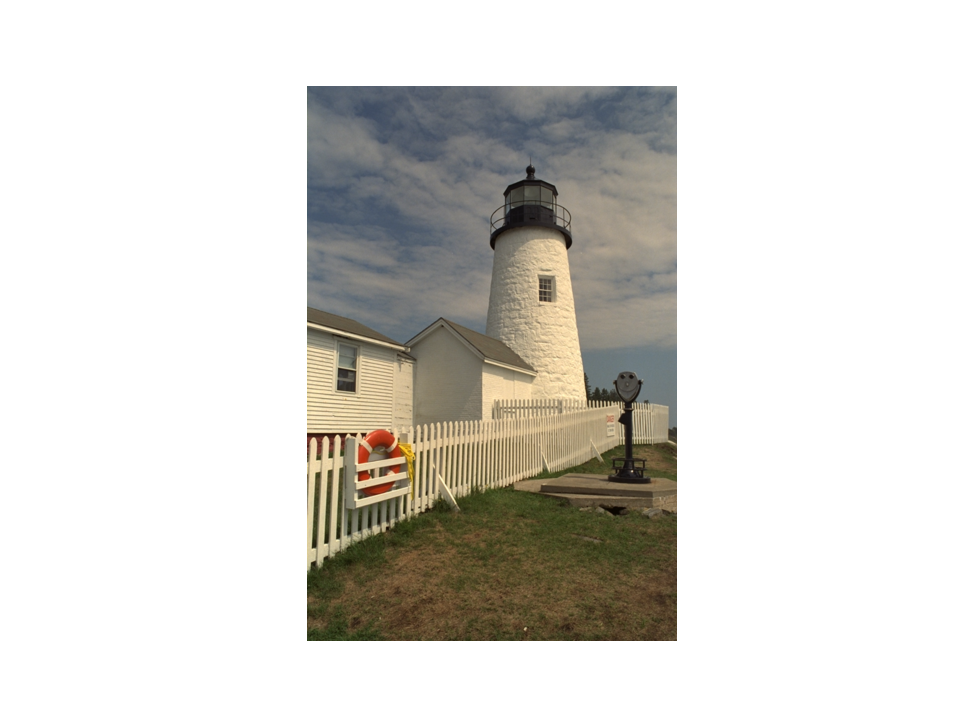
\includegraphics[trim=5cm 1.5cm 5cm 1.7cm, clip, width=1\textwidth]{figures/kodim19_original.pdf}
        \vspace{-6pt}
        \caption*{\tiny}
	\end{subfigure}%
	\begin{subfigure}{.19\textwidth}
		\centering
        \text{\small JPEG}
		\includegraphics[trim=5cm 1.5cm 5cm 1.7cm, clip, width=1\textwidth]{figures/kodim19_JPEG_bpp_0.202.pdf}
        \vspace{-15pt}
        \caption*{\tiny \textbf{PSNR: 23.00 \\ bpp: 0.20}}
	\end{subfigure}
    \begin{subfigure}{.19\textwidth}
		\centering
        \text{\small SVD}
		\includegraphics[trim=5cm 1.5cm 5cm 1.7cm, clip, width=1\textwidth]{figures/kodim19_SVD_bpp_0.215.pdf}
        \vspace{-15pt}
        \caption*{\tiny \textbf{PSNR: 21.53 \\ bpp: 0.21}}
	\end{subfigure}
    \begin{subfigure}{.19\textwidth}
		\centering
        \text{\small IMF - YC\textsubscript{B}C\textsubscript{R}}
		\includegraphics[trim=5cm 1.5cm 5cm 1.7cm, clip, width=1\textwidth]{figures/kodim19_IMF_bpp_0.191.pdf}
        \vspace{-15pt}
        \caption*{\tiny \textbf{PSNR: 24.32 \\ bpp: 0.19}}
	\end{subfigure}
    \begin{subfigure}{.19\textwidth}
		\centering
        \text{\small IMF - RGB}
		\includegraphics[trim=5cm 1.5cm 5cm 1.7cm, clip, width=1\textwidth]{figures/kodim19_IMF - RGB_bpp_0.247.pdf}
        \vspace{-15pt}
        \caption*{\tiny \textbf{PSNR: 25.40 \\ bpp: 0.24}}
	\end{subfigure}
    \caption{Qualitative performance comparison on an image from Kodak.}
	\label{fig:qualitative_comparison_kodim19}
\end{figure}

\section{Structural Similarity Index Measure (SSIM) Metrics}
In Figures \ref{fig:compression_performance_ssim} and \ref{fig: ablation studies: ssim}, average SSIM values for the images of the Kodak and CLIC datasets are presented. 

\begin{figure}[t]
	\centering
	\begin{subfigure}{.45\textwidth}
		\centering
		\includegraphics[width=.95\textwidth]{figures/comparison_kodak_ssim.pdf}
		\caption{performance on Kodak}
		\label{fig: ssim-vs-bpp kodak}
	\end{subfigure}%
	\begin{subfigure}{.45\textwidth}
		\centering
		\includegraphics[width=.95\textwidth]{figures/comparison_clic_ssim.pdf}
		\caption{performance on CLIC}
		\label{fig: ssim-vs-bpp clic}
	\end{subfigure}
	\caption{Performance comparison of JPEG, SVD, and IMF compression algorithms on Kodak and CLIC.}
	\label{fig:compression_performance_ssim}
\end{figure}

\begin{figure}[t]
	\centering
	\begin{subfigure}{.45\textwidth}
		\centering
		\includegraphics[width=.95\textwidth]{figures/ablation_patchsize_ssim.pdf}
		\caption{ablation on patch size}
		\label{fig: patch ablation ssim-vs-bpp}
	\end{subfigure}%
	\begin{subfigure}{.45\textwidth}
		\centering
		\includegraphics[width=.95\textwidth]{figures/ablation_bounds_ssim.pdf}
		\caption{ablation on factor bounds}
		\label{fig: bounds ablation ssim-vs-bpp}
	\end{subfigure}
    \begin{subfigure}{.45\textwidth}
		\centering
		\includegraphics[width=.95\textwidth]{figures/ablation_iternum_ssim.pdf}
		\caption{ablation on BCD iteration number}
		\label{fig: iteration ablation ssim-vs-bpp}
	\end{subfigure}%
	\begin{subfigure}{.45\textwidth}
		\centering
		\includegraphics[width=.95\textwidth]{figures/ablation_colorspace_ssim.pdf}
		\caption{ablation on color space}
		\label{fig: colorspace ablation ssim-vs-bpp}
	\end{subfigure}
	\caption{Ablation studies for IMF. Average SSIM on the Kodak dataset is reported versus bpp. 
    }
	\label{fig: ablation studies: ssim}
\end{figure}


%%%%%%%%%%%%%%%%%%%%%%%%%%%%%%%%%%%%%%%%%%%%%%%%%%%%%%%%%%%%

\end{document}